\documentclass[twoside]{book}

% Packages required by doxygen
\usepackage{fixltx2e}
\usepackage{calc}
\usepackage{doxygen}
\usepackage[export]{adjustbox} % also loads graphicx
\usepackage{graphicx}
\usepackage[utf8]{inputenc}
\usepackage{makeidx}
\usepackage{multicol}
\usepackage{multirow}
\PassOptionsToPackage{warn}{textcomp}
\usepackage{textcomp}
\usepackage[nointegrals]{wasysym}
\usepackage[table]{xcolor}

% Font selection
\usepackage[T1]{fontenc}
\usepackage[scaled=.90]{helvet}
\usepackage{courier}
\usepackage{amssymb}
\usepackage{sectsty}
\renewcommand{\familydefault}{\sfdefault}
\allsectionsfont{%
  \fontseries{bc}\selectfont%
  \color{darkgray}%
}
\renewcommand{\DoxyLabelFont}{%
  \fontseries{bc}\selectfont%
  \color{darkgray}%
}
\newcommand{\+}{\discretionary{\mbox{\scriptsize$\hookleftarrow$}}{}{}}

% Page & text layout
\usepackage{geometry}
\geometry{%
  a4paper,%
  top=2.5cm,%
  bottom=2.5cm,%
  left=2.5cm,%
  right=2.5cm%
}
\tolerance=750
\hfuzz=15pt
\hbadness=750
\setlength{\emergencystretch}{15pt}
\setlength{\parindent}{0cm}
\setlength{\parskip}{3ex plus 2ex minus 2ex}
\makeatletter
\renewcommand{\paragraph}{%
  \@startsection{paragraph}{4}{0ex}{-1.0ex}{1.0ex}{%
    \normalfont\normalsize\bfseries\SS@parafont%
  }%
}
\renewcommand{\subparagraph}{%
  \@startsection{subparagraph}{5}{0ex}{-1.0ex}{1.0ex}{%
    \normalfont\normalsize\bfseries\SS@subparafont%
  }%
}
\makeatother

% Headers & footers
\usepackage{fancyhdr}
\pagestyle{fancyplain}
\fancyhead[LE]{\fancyplain{}{\bfseries\thepage}}
\fancyhead[CE]{\fancyplain{}{}}
\fancyhead[RE]{\fancyplain{}{\bfseries\leftmark}}
\fancyhead[LO]{\fancyplain{}{\bfseries\rightmark}}
\fancyhead[CO]{\fancyplain{}{}}
\fancyhead[RO]{\fancyplain{}{\bfseries\thepage}}
\fancyfoot[LE]{\fancyplain{}{}}
\fancyfoot[CE]{\fancyplain{}{}}
\fancyfoot[RE]{\fancyplain{}{\bfseries\scriptsize Generated by Doxygen }}
\fancyfoot[LO]{\fancyplain{}{\bfseries\scriptsize Generated by Doxygen }}
\fancyfoot[CO]{\fancyplain{}{}}
\fancyfoot[RO]{\fancyplain{}{}}
\renewcommand{\footrulewidth}{0.4pt}
\renewcommand{\chaptermark}[1]{%
  \markboth{#1}{}%
}
\renewcommand{\sectionmark}[1]{%
  \markright{\thesection\ #1}%
}

% Indices & bibliography
\usepackage{natbib}
\usepackage[titles]{tocloft}
\setcounter{tocdepth}{3}
\setcounter{secnumdepth}{5}
\makeindex

% Hyperlinks (required, but should be loaded last)
\usepackage{ifpdf}
\ifpdf
  \usepackage[pdftex,pagebackref=true]{hyperref}
\else
  \usepackage[ps2pdf,pagebackref=true]{hyperref}
\fi
\hypersetup{%
  colorlinks=true,%
  linkcolor=blue,%
  citecolor=blue,%
  unicode%
}

% Custom commands
\newcommand{\clearemptydoublepage}{%
  \newpage{\pagestyle{empty}\cleardoublepage}%
}

\usepackage{caption}
\captionsetup{labelsep=space,justification=centering,font={bf},singlelinecheck=off,skip=4pt,position=top}

%===== C O N T E N T S =====

\begin{document}

% Titlepage & ToC
\hypersetup{pageanchor=false,
             bookmarksnumbered=true,
             pdfencoding=unicode
            }
\pagenumbering{alph}
\begin{titlepage}
\vspace*{7cm}
\begin{center}%
{\Large H\+I\+PE }\\
\vspace*{1cm}
{\large Generated by Doxygen 1.8.14}\\
\end{center}
\end{titlepage}
\clearemptydoublepage
\pagenumbering{roman}
\tableofcontents
\clearemptydoublepage
\pagenumbering{arabic}
\hypersetup{pageanchor=true}

%--- Begin generated contents ---
\chapter{Web\+R\+TC Native Video Recorder}
\label{md_source_webrtcrecorder__r_e_a_d_m_e}
\Hypertarget{md_source_webrtcrecorder__r_e_a_d_m_e}
This sample app showcases how to record live Web\+R\+TC video streams on the server side using Lib\+Sourcey. Audio and video streams are recorded and multiplexed in M\+P4 format (H.\+264/\+A\+CC) by default, but any format supported by Lib\+Sourcey/\+F\+Fmpeg can be used.

\subsection*{Installation}


\begin{DoxyEnumerate}
\item Compile Lib\+Sourcey with Web\+R\+TC support ({\ttfamily W\+I\+T\+H\+\_\+\+W\+E\+B\+R\+TC=ON}) and samples ({\ttfamily B\+U\+I\+L\+D\+\_\+\+S\+A\+M\+P\+L\+E\+S\+\_\+webrtc=ON}) enabled. See the main R\+E\+A\+D\+ME for help\+: \href{https://github.com/sourcey/libsourcey#installing-on-linux}{\tt https\+://github.\+com/sourcey/libsourcey\#installing-\/on-\/linux}
\item Run the {\ttfamily webrtcrecorder} sample application from the {\ttfamily build} directory.
\end{DoxyEnumerate}
\begin{DoxyEnumerate}
\item Install and run the Node.\+js client application\+:
\end{DoxyEnumerate}


\begin{DoxyCode}
cd <libsourcey>/src/webrtc/samples/webrtcrecorder/client
npm install
node app
\end{DoxyCode}



\begin{DoxyEnumerate}
\item Finally, point your browser to\+: {\ttfamily \href{http://localhost:4499}{\tt http\+://localhost\+:4499}}
\item Your Web\+R\+TC stream will be recorded as {\ttfamily webrtcrecorder.\+mp4}.
\end{DoxyEnumerate}

\subsection*{Hacking}

The source code is clear and concise, let it be your guide \+:) 
\chapter{Symple Web\+R\+TC Video Chat Demo}
\label{md_source_webrtcstreamer_client__r_e_a_d_m_e}
\Hypertarget{md_source_webrtcstreamer_client__r_e_a_d_m_e}
The Symple video chat demo is an example of how to use the Symple for instant messaging and Web\+R\+TC signaling in about 100 lines of Java\+Script. External projects used are Angular\+JS, Bootstrap, Node.\+js and Express.

See this blog post for more information about the demo\+: \href{http://sourcey.com/symple-webrtc-video-chat-demo}{\tt http\+://sourcey.\+com/symple-\/webrtc-\/video-\/chat-\/demo}

\subsection*{What is Symple?}

Symple is a unrestrictive real-\/time messaging and presence protocol.

The protocol itself is semantically similar to X\+M\+PP, except that it is much more flexible and economical due to the use of J\+S\+ON instead of X\+ML for encoding messages.

Symple currently has client implementations in \href{https://github.com/sourcey/symple-client}{\tt Java\+Script}, \href{https://github.com/sourcey/symple-client-ruby}{\tt Ruby} and \href{https://github.com/sourcey/libsourcey/tree/master/src/symple}{\tt C++}, which make it ideal for a wide range of messaging requirements, such as building real-\/time games and applications which run in the web browser, desktop, and mobile phone.

\subsection*{Usage}


\begin{DoxyEnumerate}
\item Install dependencies\+: {\ttfamily npm install}
\item Fire up the server\+: {\ttfamily node app}
\item And point your browser to\+: {\ttfamily \href{http://localhost:4500}{\tt http\+://localhost\+:4500}}
\end{DoxyEnumerate}

\subsection*{Hacking}

Some key options are specified in the main H\+T\+ML file located at {\ttfamily index.\+ejs}

{\bfseries C\+L\+I\+E\+N\+T\+\_\+\+O\+P\+T\+I\+O\+NS} This is the options hash for the Symple client. This is where you specify the server U\+RL and Peer object. Note that we have disabled \textquotesingle{}websocket\textquotesingle{} transport by default, but you will probably want to re-\/enable it in production.

{\bfseries W\+E\+B\+R\+T\+C\+\_\+\+C\+O\+N\+F\+IG} This is the Peer\+Connection options hash. In production you will want to specify some T\+U\+RN servers so as to ensure the p2p connection succeeds in all network topologies.

Other than that all relevant Java\+Script is located in {\ttfamily public/js/app.\+js} and {\ttfamily public/js/helpers.\+js}. Enjoy!

\subsection*{Contributing}


\begin{DoxyEnumerate}
\item Fork it
\item Create your feature branch ({\ttfamily git checkout -\/b my-\/new-\/feature})
\item Commit your changes ({\ttfamily git commit -\/am \textquotesingle{}Add some feature\textquotesingle{}})
\item Push to the branch ({\ttfamily git push origin my-\/new-\/feature})
\item Create new Pull Request
\end{DoxyEnumerate}

\subsection*{Contact}

For more information please check out the Symple homepage\+: \href{http://sourcey.com/symple/}{\tt http\+://sourcey.\+com/symple/} If you have a bug or an issue then please use the Github issue tracker\+: \href{https://github.com/sourcey/symple-client/issues}{\tt https\+://github.\+com/sourcey/symple-\/client/issues} 
\chapter{Web\+R\+TC Native Video Recorder}
\label{md_source_webrtcstreamer__r_e_a_d_m_e}
\Hypertarget{md_source_webrtcstreamer__r_e_a_d_m_e}
This sample app showcases how to stream realtime video to the the browser using Lib\+Sourcey and Web\+R\+TC. Audio and video streams can be from realtime device captures or movie files encoded in any format that\textquotesingle{}s supported by Lib\+Sourcey/\+F\+Fmpeg.

\subsection*{Installation}


\begin{DoxyEnumerate}
\item Compile Lib\+Sourcey with Web\+R\+TC support ({\ttfamily W\+I\+T\+H\+\_\+\+W\+E\+B\+R\+TC=ON}) and samples ({\ttfamily B\+U\+I\+L\+D\+\_\+\+S\+A\+M\+P\+L\+E\+S\+\_\+webrtc=ON}) enabled. See the main R\+E\+A\+D\+ME for help\+: \href{https://github.com/sourcey/libsourcey#installing-on-linux}{\tt https\+://github.\+com/sourcey/libsourcey\#installing-\/on-\/linux}
\item Run the {\ttfamily webrtcstreamer} sample application from the {\ttfamily build} directory.
\end{DoxyEnumerate}
\begin{DoxyEnumerate}
\item Install and run the Node.\+js client application\+:
\end{DoxyEnumerate}


\begin{DoxyCode}
cd <libsourcey>/src/webrtc/samples/webrtcstreamer/client
npm install
node app
\end{DoxyCode}



\begin{DoxyEnumerate}
\item Finally, point your browser to\+: {\ttfamily \href{http://localhost:4499}{\tt http\+://localhost\+:4499}}
\item Your should see your video and audio stream playing in the browser.
\end{DoxyEnumerate}

\subsection*{Hacking}

The source code is clear and concise, let it be your guide \+:) 
\chapter{Todo List}
\label{todo}
\Hypertarget{todo}

\begin{DoxyRefList}
\item[\label{todo__todo000001}%
\Hypertarget{todo__todo000001}%
Class \hyperlink{classfilter_1_1algos_1_1_akaze}{filter\+:\+:algos\+:\+:Akaze} ]
\item[\label{todo__todo000007}%
\Hypertarget{todo__todo000007}%
Member \hyperlink{classfilter_1_1algos_1_1_cropper_1_1_c_v_cropper_data_a8f2195d489fd541b9add781355bc99c2}{filter\+:\+:algos\+:\+:Cropper\+:\+:C\+V\+Cropper\+Data\+:\+:C\+V\+Cropper\+Data} (const \hyperlink{classfilter_1_1data_1_1_pattern_data}{data\+::\+Pattern\+Data} \&pat)]
\item[\label{todo__todo000006}%
\Hypertarget{todo__todo000006}%
Member \hyperlink{classfilter_1_1algos_1_1_cropper_ac7cf2a54e81d9227dc22b46d54603c7e}{filter\+:\+:algos\+:\+:Cropper\+:\+:wait} ]
\item[\label{todo__todo000008}%
\Hypertarget{todo__todo000008}%
Class \hyperlink{classfilter_1_1algos_1_1_face_detection}{filter\+:\+:algos\+:\+:Face\+Detection} ]
\item[\label{todo__todo000009}%
\Hypertarget{todo__todo000009}%
Class \hyperlink{classfilter_1_1algos_1_1_face_landmark}{filter\+:\+:algos\+:\+:Face\+Landmark} ]
\item[\label{todo__todo000010}%
\Hypertarget{todo__todo000010}%
Class \hyperlink{classfilter_1_1algos_1_1_latch}{filter\+:\+:algos\+:\+:Latch} ]
\item[\label{todo__todo000011}%
\Hypertarget{todo__todo000011}%
Class \hyperlink{classfilter_1_1algos_1_1_overlay_filter}{filter\+:\+:algos\+:\+:Overlay\+Filter} ]
\item[\label{todo__todo000012}%
\Hypertarget{todo__todo000012}%
Class \hyperlink{classfilter_1_1algos_1_1_overlay_mat_filter}{filter\+:\+:algos\+:\+:Overlay\+Mat\+Filter} ]
\item[\label{todo__todo000013}%
\Hypertarget{todo__todo000013}%
Class \hyperlink{classfilter_1_1algos_1_1_result_filter}{filter\+:\+:algos\+:\+:Result\+Filter} ]
\item[\label{todo__todo000014}%
\Hypertarget{todo__todo000014}%
Class \hyperlink{classfilter_1_1algos_1_1_show_image}{filter\+:\+:algos\+:\+:Show\+Image} ]
\item[\label{todo__todo000015}%
\Hypertarget{todo__todo000015}%
Class \hyperlink{classfilter_1_1algos_1_1_show_video}{filter\+:\+:algos\+:\+:Show\+Video} ]
\item[\label{todo__todo000016}%
\Hypertarget{todo__todo000016}%
Class \hyperlink{classfilter_1_1algos_1_1_stream_result_filter}{filter\+:\+:algos\+:\+:Stream\+Result\+Filter} ]
\item[\label{todo__todo000002}%
\Hypertarget{todo__todo000002}%
Class \hyperlink{structfilter_1_1_algos_1_1_user_data}{filter\+:\+:Algos\+:\+:User\+Data} ]
\item[\label{todo__todo000017}%
\Hypertarget{todo__todo000017}%
Class \hyperlink{classfilter_1_1data_1_1_composer}{filter\+:\+:data\+:\+:Composer} ]
\item[\label{todo__todo000019}%
\Hypertarget{todo__todo000019}%
Class \hyperlink{classfilter_1_1data_1_1_data_port}{filter\+:\+:data\+:\+:Data\+Port} ]
\item[\label{todo__todo000018}%
\Hypertarget{todo__todo000018}%
Class \hyperlink{classfilter_1_1data_1_1_data_port_base}{filter\+:\+:data\+:\+:Data\+Port\+Base} ]
\item[\label{todo__todo000020}%
\Hypertarget{todo__todo000020}%
Member \hyperlink{classfilter_1_1data_1_1_file_image_data_abd280bc0cc3d1a1e6aa1924041a71820}{filter\+:\+:data\+:\+:File\+Image\+Data\+:\+:operator=} (const \hyperlink{classfilter_1_1data_1_1_file_image_data}{File\+Image\+Data} \&left)]
\item[\label{todo__todo000021}%
\Hypertarget{todo__todo000021}%
Member \hyperlink{classfilter_1_1data_1_1_file_video_input_a7db00de01c31e63d49a518e737ab8799}{filter\+:\+:data\+:\+:File\+Video\+Input\+:\+:empty} () const]
\item[\label{todo__todo000022}%
\Hypertarget{todo__todo000022}%
Member \hyperlink{classfilter_1_1data_1_1_image_array_data_a6986bd7246e4468bf9afd2c2196608fc}{filter\+:\+:data\+:\+:Image\+Array\+Data\+:\+:operator=} (const \hyperlink{classfilter_1_1data_1_1_image_array_data}{Image\+Array\+Data} \&left)]
\item[\label{todo__todo000024}%
\Hypertarget{todo__todo000024}%
Class \hyperlink{classfilter_1_1data_1_1_i_o_data}{filter\+:\+:data\+:\+:I\+O\+Data$<$ Base, Derived $>$} ]
\item[\label{todo__todo000025}%
\Hypertarget{todo__todo000025}%
Class \hyperlink{classfilter_1_1data_1_1_output_data}{filter\+:\+:data\+:\+:Output\+Data} ]
\item[\label{todo__todo000026}%
\Hypertarget{todo__todo000026}%
Member \hyperlink{classfilter_1_1data_1_1_pattern_data_aa01d481a29ec5690914612fb0b39e997}{filter\+:\+:data\+:\+:Pattern\+Data\+:\+:operator$<$$<$} (const \hyperlink{classfilter_1_1data_1_1_pattern_data}{Pattern\+Data} \&left)]
\item[\label{todo__todo000027}%
\Hypertarget{todo__todo000027}%
Class \hyperlink{classfilter_1_1_i_filter}{filter\+:\+:I\+Filter} ]
\item[\label{todo__todo000028}%
\Hypertarget{todo__todo000028}%
Class \hyperlink{classfilter_1_1_model}{filter\+:\+:Model} ]
\end{DoxyRefList}
\chapter{Hierarchical Index}
\section{Class Hierarchy}
This inheritance list is sorted roughly, but not completely, alphabetically\+:\begin{DoxyCompactList}
\item \contentsline{section}{filter\+:\+:data\+:\+:I\+O\+Data$<$ Base, Derived $>$\+:\+:\+\_\+\+Protection}{\pageref{classfilter_1_1data_1_1_i_o_data_1_1___protection}}{}
\item Application\begin{DoxyCompactList}
\item \contentsline{section}{scy\+:\+:Signaler}{\pageref{classscy_1_1_signaler}}{}
\item \contentsline{section}{scy\+:\+:Signaler}{\pageref{classscy_1_1_signaler}}{}
\end{DoxyCompactList}
\item \contentsline{section}{dt\+Functor\+:\+:base}{\pageref{structdt_functor_1_1base}}{}
\begin{DoxyCompactList}
\item \contentsline{section}{dt\+Functor\+:\+:wrapped$<$ Obj, Args $>$}{\pageref{structdt_functor_1_1wrapped}}{}
\end{DoxyCompactList}
\item \contentsline{section}{Simple\+Web\+:\+:Crypto\+:\+:Base64}{\pageref{class_simple_web_1_1_crypto_1_1_base64}}{}
\item \contentsline{section}{Base\+Singleton}{\pageref{class_base_singleton}}{}
\begin{DoxyCompactList}
\item \contentsline{section}{Singleton$<$ T $>$}{\pageref{class_singleton}}{}
\item \contentsline{section}{Singleton$<$ Capture\+Video\+Factory $>$}{\pageref{class_singleton}}{}
\begin{DoxyCompactList}
\item \contentsline{section}{Capture\+Video\+Factory}{\pageref{class_capture_video_factory}}{}
\end{DoxyCompactList}
\item \contentsline{section}{Singleton$<$ Orchestrator\+Factory $>$}{\pageref{class_singleton}}{}
\begin{DoxyCompactList}
\item \contentsline{section}{orchestrator\+:\+:Orchestrator\+Factory}{\pageref{classorchestrator_1_1_orchestrator_factory}}{}
\end{DoxyCompactList}
\item \contentsline{section}{Singleton$<$ Streaming $>$}{\pageref{class_singleton}}{}
\begin{DoxyCompactList}
\item \contentsline{section}{Streaming}{\pageref{class_streaming}}{}
\end{DoxyCompactList}
\end{DoxyCompactList}
\item \contentsline{section}{Capture\+Video}{\pageref{class_capture_video}}{}
\begin{DoxyCompactList}
\item \contentsline{section}{R\+T\+S\+P\+Capture}{\pageref{class_r_t_s_p_capture}}{}
\end{DoxyCompactList}
\item \contentsline{section}{http\+:\+:Client\+Base$<$ socket\+\_\+type $>$}{\pageref{classhttp_1_1_client_base}}{}
\begin{DoxyCompactList}
\item \contentsline{section}{http\+:\+:Client$<$ socket\+\_\+type $>$}{\pageref{classhttp_1_1_client}}{}
\end{DoxyCompactList}
\item \contentsline{section}{http\+:\+:Client\+Base$<$ H\+T\+TP $>$}{\pageref{classhttp_1_1_client_base}}{}
\begin{DoxyCompactList}
\item \contentsline{section}{http\+:\+:Client$<$ H\+T\+TP $>$}{\pageref{classhttp_1_1_client_3_01_h_t_t_p_01_4}}{}
\end{DoxyCompactList}
\item \contentsline{section}{filter\+:\+:algos\+:\+:Closest\+Color\+:\+:Color}{\pageref{structfilter_1_1algos_1_1_closest_color_1_1_color}}{}
\item \contentsline{section}{http\+:\+:Command\+Executer}{\pageref{classhttp_1_1_command_executer}}{}
\item \contentsline{section}{http\+:\+:Command\+Manager}{\pageref{classhttp_1_1_command_manager}}{}
\item \contentsline{section}{filter\+:\+:algos\+:\+:I\+D\+Plate\+:\+:Compare\+By\+Deriv}{\pageref{structfilter_1_1algos_1_1_i_d_plate_1_1_compare_by_deriv}}{}
\item \contentsline{section}{filter\+:\+:data\+:\+:Composer}{\pageref{classfilter_1_1data_1_1_composer}}{}
\item \contentsline{section}{filter\+:\+:algos\+:\+:I\+D\+Plate\+:\+:Comp\+Rects\+By\+Pos}{\pageref{structfilter_1_1algos_1_1_i_d_plate_1_1_comp_rects_by_pos}}{}
\item \contentsline{section}{core\+:\+:queue\+:\+:Concurrent\+Queue$<$ Data $>$}{\pageref{classcore_1_1queue_1_1_concurrent_queue}}{}
\item \contentsline{section}{core\+:\+:queue\+:\+:Concurrent\+Queue$<$ cv\+:\+:Mat $>$}{\pageref{classcore_1_1queue_1_1_concurrent_queue}}{}
\item \contentsline{section}{core\+:\+:queue\+:\+:Concurrent\+Queue$<$ filter\+:\+:algos\+:\+:Latch\+:\+:Match\+Container $>$}{\pageref{classcore_1_1queue_1_1_concurrent_queue}}{}
\item \contentsline{section}{core\+:\+:queue\+:\+:Concurrent\+Queue$<$ filter\+:\+:data\+:\+:Data $>$}{\pageref{classcore_1_1queue_1_1_concurrent_queue}}{}
\item \contentsline{section}{core\+:\+:queue\+:\+:Concurrent\+Queue$<$ filter\+:\+:data\+:\+:Image\+Data $>$}{\pageref{classcore_1_1queue_1_1_concurrent_queue}}{}
\item \contentsline{section}{core\+:\+:queue\+:\+:Concurrent\+Queue$<$ filter\+:\+:data\+:\+:Pattern\+Data $>$}{\pageref{classcore_1_1queue_1_1_concurrent_queue}}{}
\item \contentsline{section}{core\+:\+:queue\+:\+:Concurrent\+Queue$<$ filter\+:\+:data\+:\+:Square\+Crop $>$}{\pageref{classcore_1_1queue_1_1_concurrent_queue}}{}
\item \contentsline{section}{core\+:\+:queue\+:\+:Concurrent\+Queue$<$ std\+:\+:vector$<$ cv\+:\+:Point $>$ $>$}{\pageref{classcore_1_1queue_1_1_concurrent_queue}}{}
\item \contentsline{section}{orchestrator\+:\+:Conductor}{\pageref{classorchestrator_1_1_conductor}}{}
\begin{DoxyCompactList}
\item \contentsline{section}{orchestrator\+:\+:image\+:\+:Default\+Scheduler}{\pageref{classorchestrator_1_1image_1_1_default_scheduler}}{}
\end{DoxyCompactList}
\item \contentsline{section}{http\+:\+:Server\+Base$<$ socket\+\_\+type $>$\+:\+:Config}{\pageref{classhttp_1_1_server_base_1_1_config}}{}
\item \contentsline{section}{F\+Fmpeg\+Opencv\+Decoder\+:\+:config}{\pageref{struct_f_fmpeg_opencv_decoder_1_1config}}{}
\item \contentsline{section}{http\+:\+:Config}{\pageref{classhttp_1_1_config}}{}
\item \contentsline{section}{http\+:\+:Client\+Base$<$ socket\+\_\+type $>$\+:\+:Config}{\pageref{classhttp_1_1_client_base_1_1_config}}{}
\item \contentsline{section}{filter\+:\+:data\+:\+:Connex\+Data\+Base}{\pageref{classfilter_1_1data_1_1_connex_data_base}}{}
\begin{DoxyCompactList}
\item \contentsline{section}{filter\+:\+:data\+:\+:Connex\+Data$<$ Din, Din $>$}{\pageref{classfilter_1_1data_1_1_connex_data}}{}
\begin{DoxyCompactList}
\item \contentsline{section}{filter\+:\+:data\+:\+:Connex\+Input$<$ Din $>$}{\pageref{classfilter_1_1data_1_1_connex_input}}{}
\end{DoxyCompactList}
\item \contentsline{section}{filter\+:\+:data\+:\+:Connex\+Data$<$ Dout, Dout $>$}{\pageref{classfilter_1_1data_1_1_connex_data}}{}
\begin{DoxyCompactList}
\item \contentsline{section}{filter\+:\+:data\+:\+:Connex\+Output$<$ Dout $>$}{\pageref{classfilter_1_1data_1_1_connex_output}}{}
\end{DoxyCompactList}
\item \contentsline{section}{filter\+:\+:data\+:\+:Connex\+Data$<$ filter\+:\+:data\+:\+:Data, filter\+:\+:data\+:\+:Data $>$}{\pageref{classfilter_1_1data_1_1_connex_data}}{}
\begin{DoxyCompactList}
\item \contentsline{section}{filter\+:\+:data\+:\+:Connex\+Input$<$ filter\+:\+:data\+:\+:Data $>$}{\pageref{classfilter_1_1data_1_1_connex_input}}{}
\item \contentsline{section}{filter\+:\+:data\+:\+:Connex\+Output$<$ filter\+:\+:data\+:\+:Data $>$}{\pageref{classfilter_1_1data_1_1_connex_output}}{}
\end{DoxyCompactList}
\item \contentsline{section}{filter\+:\+:data\+:\+:Connex\+Data$<$ filter\+:\+:data\+:\+:Data, filter\+:\+:data\+:\+:Image\+Data $>$}{\pageref{classfilter_1_1data_1_1_connex_data}}{}
\item \contentsline{section}{filter\+:\+:data\+:\+:Connex\+Data$<$ filter\+:\+:data\+:\+:Image\+Array\+Data, filter\+:\+:data\+:\+:Image\+Array\+Data $>$}{\pageref{classfilter_1_1data_1_1_connex_data}}{}
\item \contentsline{section}{filter\+:\+:data\+:\+:Connex\+Data$<$ filter\+:\+:data\+:\+:Image\+Array\+Data, filter\+:\+:data\+:\+:Image\+Data $>$}{\pageref{classfilter_1_1data_1_1_connex_data}}{}
\item \contentsline{section}{filter\+:\+:data\+:\+:Connex\+Data$<$ filter\+:\+:data\+:\+:Image\+Array\+Data, filter\+:\+:data\+:\+:Square\+Crop $>$}{\pageref{classfilter_1_1data_1_1_connex_data}}{}
\item \contentsline{section}{filter\+:\+:data\+:\+:Connex\+Data$<$ filter\+:\+:data\+:\+:Image\+Data, filter\+:\+:data\+:\+:Image\+Array\+Data $>$}{\pageref{classfilter_1_1data_1_1_connex_data}}{}
\item \contentsline{section}{filter\+:\+:data\+:\+:Connex\+Data$<$ filter\+:\+:data\+:\+:Image\+Data, filter\+:\+:data\+:\+:Image\+Data $>$}{\pageref{classfilter_1_1data_1_1_connex_data}}{}
\begin{DoxyCompactList}
\item \contentsline{section}{filter\+:\+:data\+:\+:Connex\+Output$<$ filter\+:\+:data\+:\+:Image\+Data $>$}{\pageref{classfilter_1_1data_1_1_connex_output}}{}
\end{DoxyCompactList}
\item \contentsline{section}{filter\+:\+:data\+:\+:Connex\+Data$<$ filter\+:\+:data\+:\+:Image\+Data, filter\+:\+:data\+:\+:Pattern\+Data $>$}{\pageref{classfilter_1_1data_1_1_connex_data}}{}
\item \contentsline{section}{filter\+:\+:data\+:\+:Connex\+Data$<$ filter\+:\+:data\+:\+:Pattern\+Data, filter\+:\+:data\+:\+:Image\+Data $>$}{\pageref{classfilter_1_1data_1_1_connex_data}}{}
\item \contentsline{section}{filter\+:\+:data\+:\+:Connex\+Data$<$ filter\+:\+:data\+:\+:Pattern\+Data, filter\+:\+:data\+:\+:Pattern\+Data $>$}{\pageref{classfilter_1_1data_1_1_connex_data}}{}
\item \contentsline{section}{filter\+:\+:data\+:\+:Connex\+Data$<$ Din, Dout $>$}{\pageref{classfilter_1_1data_1_1_connex_data}}{}
\end{DoxyCompactList}
\item \contentsline{section}{filter\+:\+:data\+:\+:Copy\+Object$<$ My\+Class $>$}{\pageref{classfilter_1_1data_1_1_copy_object}}{}
\item \contentsline{section}{Simple\+Web\+:\+:Crypto}{\pageref{class_simple_web_1_1_crypto}}{}
\item \contentsline{section}{filter\+:\+:algos\+:\+:Cropper\+:\+:C\+V\+Cropper\+Data}{\pageref{classfilter_1_1algos_1_1_cropper_1_1_c_v_cropper_data}}{}
\item \contentsline{section}{filter\+:\+:data\+:\+:Data}{\pageref{classfilter_1_1data_1_1_data}}{}
\begin{DoxyCompactList}
\item \contentsline{section}{filter\+:\+:data\+:\+:I\+O\+Data$<$ Data, Derived $>$}{\pageref{classfilter_1_1data_1_1_i_o_data}}{}
\begin{DoxyCompactList}
\item \contentsline{section}{filter\+:\+:data\+:\+:Video\+Data$<$ Derived $>$}{\pageref{classfilter_1_1data_1_1_video_data}}{}
\end{DoxyCompactList}
\item \contentsline{section}{filter\+:\+:data\+:\+:I\+O\+Data$<$ Data, File\+Video\+Input $>$}{\pageref{classfilter_1_1data_1_1_i_o_data}}{}
\begin{DoxyCompactList}
\item \contentsline{section}{filter\+:\+:data\+:\+:Video\+Data$<$ File\+Video\+Input $>$}{\pageref{classfilter_1_1data_1_1_video_data}}{}
\begin{DoxyCompactList}
\item \contentsline{section}{filter\+:\+:data\+:\+:File\+Video\+Input}{\pageref{classfilter_1_1data_1_1_file_video_input}}{}
\end{DoxyCompactList}
\end{DoxyCompactList}
\item \contentsline{section}{filter\+:\+:data\+:\+:I\+O\+Data$<$ Data, Image\+Array\+Data $>$}{\pageref{classfilter_1_1data_1_1_i_o_data}}{}
\begin{DoxyCompactList}
\item \contentsline{section}{filter\+:\+:data\+:\+:Image\+Array\+Data}{\pageref{classfilter_1_1data_1_1_image_array_data}}{}
\begin{DoxyCompactList}
\item \contentsline{section}{filter\+:\+:data\+:\+:I\+O\+Data$<$ Image\+Array\+Data, Directory\+Img\+Data $>$}{\pageref{classfilter_1_1data_1_1_i_o_data}}{}
\begin{DoxyCompactList}
\item \contentsline{section}{filter\+:\+:data\+:\+:Directory\+Img\+Data}{\pageref{classfilter_1_1data_1_1_directory_img_data}}{}
\end{DoxyCompactList}
\item \contentsline{section}{filter\+:\+:data\+:\+:I\+O\+Data$<$ Image\+Array\+Data, Image\+Data $>$}{\pageref{classfilter_1_1data_1_1_i_o_data}}{}
\begin{DoxyCompactList}
\item \contentsline{section}{filter\+:\+:data\+:\+:Image\+Data}{\pageref{classfilter_1_1data_1_1_image_data}}{}
\begin{DoxyCompactList}
\item \contentsline{section}{filter\+:\+:data\+:\+:I\+O\+Data$<$ Image\+Data, File\+Image\+Data $>$}{\pageref{classfilter_1_1data_1_1_i_o_data}}{}
\item \contentsline{section}{filter\+:\+:data\+:\+:File\+Image\+Data}{\pageref{classfilter_1_1data_1_1_file_image_data}}{}
\end{DoxyCompactList}
\end{DoxyCompactList}
\item \contentsline{section}{filter\+:\+:data\+:\+:I\+O\+Data$<$ Image\+Array\+Data, Output\+Data $>$}{\pageref{classfilter_1_1data_1_1_i_o_data}}{}
\begin{DoxyCompactList}
\item \contentsline{section}{filter\+:\+:data\+:\+:Output\+Data}{\pageref{classfilter_1_1data_1_1_output_data}}{}
\end{DoxyCompactList}
\end{DoxyCompactList}
\end{DoxyCompactList}
\item \contentsline{section}{filter\+:\+:data\+:\+:I\+O\+Data$<$ Data, List\+I\+O\+Data $>$}{\pageref{classfilter_1_1data_1_1_i_o_data}}{}
\begin{DoxyCompactList}
\item \contentsline{section}{filter\+:\+:data\+:\+:List\+I\+O\+Data}{\pageref{classfilter_1_1data_1_1_list_i_o_data}}{}
\end{DoxyCompactList}
\item \contentsline{section}{filter\+:\+:data\+:\+:I\+O\+Data$<$ Data, Pattern\+Data $>$}{\pageref{classfilter_1_1data_1_1_i_o_data}}{}
\begin{DoxyCompactList}
\item \contentsline{section}{filter\+:\+:data\+:\+:Video\+Data$<$ Pattern\+Data $>$}{\pageref{classfilter_1_1data_1_1_video_data}}{}
\begin{DoxyCompactList}
\item \contentsline{section}{filter\+:\+:data\+:\+:Pattern\+Data}{\pageref{classfilter_1_1data_1_1_pattern_data}}{}
\end{DoxyCompactList}
\end{DoxyCompactList}
\item \contentsline{section}{filter\+:\+:data\+:\+:I\+O\+Data$<$ Data, Square\+Crop $>$}{\pageref{classfilter_1_1data_1_1_i_o_data}}{}
\begin{DoxyCompactList}
\item \contentsline{section}{filter\+:\+:data\+:\+:Square\+Crop}{\pageref{classfilter_1_1data_1_1_square_crop}}{}
\end{DoxyCompactList}
\item \contentsline{section}{filter\+:\+:data\+:\+:I\+O\+Data$<$ Data, Stream\+Video\+Input $>$}{\pageref{classfilter_1_1data_1_1_i_o_data}}{}
\begin{DoxyCompactList}
\item \contentsline{section}{filter\+:\+:data\+:\+:Video\+Data$<$ Stream\+Video\+Input $>$}{\pageref{classfilter_1_1data_1_1_video_data}}{}
\begin{DoxyCompactList}
\item \contentsline{section}{filter\+:\+:data\+:\+:Stream\+Video\+Input}{\pageref{classfilter_1_1data_1_1_stream_video_input}}{}
\end{DoxyCompactList}
\end{DoxyCompactList}
\item \contentsline{section}{filter\+:\+:data\+:\+:I\+O\+Data$<$ Data, Text\+Data $>$}{\pageref{classfilter_1_1data_1_1_i_o_data}}{}
\begin{DoxyCompactList}
\item \contentsline{section}{filter\+:\+:data\+:\+:Text\+Data}{\pageref{classfilter_1_1data_1_1_text_data}}{}
\end{DoxyCompactList}
\end{DoxyCompactList}
\item \contentsline{section}{Data\+Access\+Mapper}{\pageref{class_data_access_mapper}}{}
\item \contentsline{section}{filter\+:\+:data\+:\+:Data\+Port\+Base}{\pageref{classfilter_1_1data_1_1_data_port_base}}{}
\begin{DoxyCompactList}
\item \contentsline{section}{filter\+:\+:data\+:\+:Data\+Port}{\pageref{classfilter_1_1data_1_1_data_port}}{}
\end{DoxyCompactList}
\item \contentsline{section}{filter\+:\+:data\+:\+:Data\+Type\+Mapper}{\pageref{classfilter_1_1data_1_1_data_type_mapper}}{}
\item \contentsline{section}{Delegate$<$ return\+\_\+type, params $>$}{\pageref{class_delegate}}{}
\item \contentsline{section}{dt\+Functor}{\pageref{classdt_functor}}{}
\item \contentsline{section}{M\+E\+S\+AI\+:\+:F\+Fmpeg\+Decoder}{\pageref{class_m_e_s_a_i_1_1_f_fmpeg_decoder}}{}
\begin{DoxyCompactList}
\item \contentsline{section}{F\+Fmpeg\+Opencv\+Decoder}{\pageref{class_f_fmpeg_opencv_decoder}}{}
\end{DoxyCompactList}
\item \contentsline{section}{M\+E\+S\+AI\+:\+:F\+Fmpeg\+H264\+Encoder}{\pageref{class_m_e_s_a_i_1_1_f_fmpeg_h264_encoder}}{}
\item Framed\+Source\begin{DoxyCompactList}
\item \contentsline{section}{Live\+Source\+Withx264}{\pageref{class_live_source_withx264}}{}
\item \contentsline{section}{M\+E\+S\+AI\+:\+:F\+Fmpeg\+H264\+Source}{\pageref{class_m_e_s_a_i_1_1_f_fmpeg_h264_source}}{}
\end{DoxyCompactList}
\item \contentsline{section}{M\+E\+S\+AI\+:\+:Frame\+Structure}{\pageref{class_m_e_s_a_i_1_1_frame_structure}}{}
\item \contentsline{section}{http\+:\+:Command\+Manager\+:\+:function\+\_\+traits$<$ T $>$}{\pageref{structhttp_1_1_command_manager_1_1function__traits}}{}
\item \contentsline{section}{http\+:\+:Command\+Manager\+:\+:function\+\_\+traits$<$ Return\+Type($\ast$)(Args ...)$>$}{\pageref{structhttp_1_1_command_manager_1_1function__traits_3_01_return_type_07_5_08_07_args_01_8_8_8_08_4}}{}
\item \contentsline{section}{http\+:\+:Command\+Manager\+:\+:function\+\_\+traits$<$ Return\+Type(Class\+Type\+:\+:$\ast$)(Args ...) const $>$}{\pageref{structhttp_1_1_command_manager_1_1function__traits_3_01_return_type_07_class_type_1_1_5_08_07_args_01_8_8_8_08_01const_01_4}}{}
\item \contentsline{section}{http\+:\+:Command\+Manager\+:\+:function\+\_\+traits$<$ Return\+Type(Class\+Type\+:\+:$\ast$)(Args ...)$>$}{\pageref{structhttp_1_1_command_manager_1_1function__traits_3_01_return_type_07_class_type_1_1_5_08_07_args_01_8_8_8_08_4}}{}
\item \contentsline{section}{http\+:\+:Http\+Params}{\pageref{classhttp_1_1_http_params}}{}
\item \contentsline{section}{http\+:\+:Http\+Request}{\pageref{classhttp_1_1_http_request}}{}
\item \contentsline{section}{http\+:\+:Http\+Task}{\pageref{classhttp_1_1_http_task}}{}
\item \contentsline{section}{http\+:\+:Server\+Base$<$ socket\+\_\+type $>$\+:\+:Request\+:\+:iequal\+\_\+to}{\pageref{classhttp_1_1_server_base_1_1_request_1_1iequal__to}}{}
\item \contentsline{section}{http\+:\+:Request$<$ socket\+\_\+type $>$\+:\+:iequal\+\_\+to}{\pageref{classhttp_1_1_request_1_1iequal__to}}{}
\item \contentsline{section}{http\+:\+:Client\+Base$<$ socket\+\_\+type $>$\+:\+:Response\+:\+:iequal\+\_\+to}{\pageref{classhttp_1_1_client_base_1_1_response_1_1iequal__to}}{}
\item \contentsline{section}{http\+:\+:Server\+Base$<$ socket\+\_\+type $>$\+:\+:Request\+:\+:ihash}{\pageref{classhttp_1_1_server_base_1_1_request_1_1ihash}}{}
\item \contentsline{section}{http\+:\+:Request$<$ socket\+\_\+type $>$\+:\+:ihash}{\pageref{classhttp_1_1_request_1_1ihash}}{}
\item \contentsline{section}{http\+:\+:Client\+Base$<$ socket\+\_\+type $>$\+:\+:Response\+:\+:ihash}{\pageref{classhttp_1_1_client_base_1_1_response_1_1ihash}}{}
\item \contentsline{section}{core\+:\+:Invoker\+Base}{\pageref{classcore_1_1_invoker_base}}{}
\begin{DoxyCompactList}
\item \contentsline{section}{core\+:\+:Invoker$<$ return\+\_\+type, params $>$}{\pageref{classcore_1_1_invoker}}{}
\end{DoxyCompactList}
\item \contentsline{section}{filter\+:\+:algos\+:\+:I\+P\+Desc}{\pageref{classfilter_1_1algos_1_1_i_p_desc}}{}
\item istream\begin{DoxyCompactList}
\item \contentsline{section}{http\+:\+:Content}{\pageref{classhttp_1_1_content}}{}
\item \contentsline{section}{http\+:\+:Server\+Base$<$ socket\+\_\+type $>$\+:\+:Content}{\pageref{classhttp_1_1_server_base_1_1_content}}{}
\end{DoxyCompactList}
\item \contentsline{section}{json\+:\+:Json\+Builder}{\pageref{classjson_1_1_json_builder}}{}
\item \contentsline{section}{json\+:\+:Json\+Filter\+Node}{\pageref{classjson_1_1_json_filter_node}}{}
\item \contentsline{section}{filter\+:\+:Algos\+:\+:Label\+O\+CR}{\pageref{classfilter_1_1_algos_1_1_label_o_c_r}}{}
\item \contentsline{section}{filter\+:\+:algos\+:\+:I\+D\+Plate\+:\+:Line\+Data}{\pageref{structfilter_1_1algos_1_1_i_d_plate_1_1_line_data}}{}
\item \contentsline{section}{M\+E\+S\+AI\+:\+:Live\+R\+T\+S\+P\+Server}{\pageref{class_m_e_s_a_i_1_1_live_r_t_s_p_server}}{}
\item \contentsline{section}{core\+:\+:Logger}{\pageref{classcore_1_1_logger}}{}
\item \contentsline{section}{filter\+:\+:algos\+:\+:Latch\+:\+:Match\+Container}{\pageref{classfilter_1_1algos_1_1_latch_1_1_match_container}}{}
\item Media\+Capture\begin{DoxyCompactList}
\item \contentsline{section}{O\+C\+V\+Video\+Capture}{\pageref{class_o_c_v_video_capture}}{}
\end{DoxyCompactList}
\item \contentsline{section}{filter\+:\+:Model}{\pageref{classfilter_1_1_model}}{}
\begin{DoxyCompactList}
\item \contentsline{section}{filter\+:\+:I\+Filter}{\pageref{classfilter_1_1_i_filter}}{}
\begin{DoxyCompactList}
\item \contentsline{section}{filter\+:\+:algos\+:\+:Akaze}{\pageref{classfilter_1_1algos_1_1_akaze}}{}
\item \contentsline{section}{filter\+:\+:Algos\+:\+:Algo\+Example\+\_\+1}{\pageref{classfilter_1_1_algos_1_1_algo_example__1}}{}
\item \contentsline{section}{filter\+:\+:algos\+:\+:Average\+Color}{\pageref{classfilter_1_1algos_1_1_average_color}}{}
\item \contentsline{section}{filter\+:\+:algos\+:\+:Bilateral\+Filter}{\pageref{classfilter_1_1algos_1_1_bilateral_filter}}{}
\item \contentsline{section}{filter\+:\+:algos\+:\+:Binary}{\pageref{classfilter_1_1algos_1_1_binary}}{}
\item \contentsline{section}{filter\+:\+:algos\+:\+:Binary\+Adaptive}{\pageref{classfilter_1_1algos_1_1_binary_adaptive}}{}
\item \contentsline{section}{filter\+:\+:algos\+:\+:Blur}{\pageref{classfilter_1_1algos_1_1_blur}}{}
\item \contentsline{section}{filter\+:\+:Algos\+:\+:Canny}{\pageref{classfilter_1_1_algos_1_1_canny}}{}
\item \contentsline{section}{filter\+:\+:algos\+:\+:Closest\+Color}{\pageref{classfilter_1_1algos_1_1_closest_color}}{}
\item \contentsline{section}{filter\+:\+:algos\+:\+:Contrast}{\pageref{classfilter_1_1algos_1_1_contrast}}{}
\item \contentsline{section}{filter\+:\+:Algos\+:\+:Crop}{\pageref{classfilter_1_1_algos_1_1_crop}}{}
\item \contentsline{section}{filter\+:\+:algos\+:\+:Cropper}{\pageref{classfilter_1_1algos_1_1_cropper}}{}
\item \contentsline{section}{filter\+:\+:algos\+:\+:Dilate}{\pageref{classfilter_1_1algos_1_1_dilate}}{}
\item \contentsline{section}{filter\+:\+:algos\+:\+:Equalize}{\pageref{classfilter_1_1algos_1_1_equalize}}{}
\item \contentsline{section}{filter\+:\+:algos\+:\+:Equalize\+Adaptive}{\pageref{classfilter_1_1algos_1_1_equalize_adaptive}}{}
\item \contentsline{section}{filter\+:\+:algos\+:\+:Erode}{\pageref{classfilter_1_1algos_1_1_erode}}{}
\item \contentsline{section}{filter\+:\+:algos\+:\+:Face\+Detection}{\pageref{classfilter_1_1algos_1_1_face_detection}}{}
\item \contentsline{section}{filter\+:\+:algos\+:\+:Face\+Landmark}{\pageref{classfilter_1_1algos_1_1_face_landmark}}{}
\item \contentsline{section}{filter\+:\+:algos\+:\+:Gaussian}{\pageref{classfilter_1_1algos_1_1_gaussian}}{}
\item \contentsline{section}{filter\+:\+:algos\+:\+:Grayscale}{\pageref{classfilter_1_1algos_1_1_grayscale}}{}
\item \contentsline{section}{filter\+:\+:algos\+:\+:I\+D\+Plate\+Cropper}{\pageref{classfilter_1_1algos_1_1_i_d_plate_cropper}}{}
\item \contentsline{section}{filter\+:\+:Algos\+:\+:I\+D\+Plate\+Identifier}{\pageref{classfilter_1_1_algos_1_1_i_d_plate_identifier}}{}
\item \contentsline{section}{filter\+:\+:algos\+:\+:I\+D\+Plate\+Rectifier}{\pageref{classfilter_1_1algos_1_1_i_d_plate_rectifier}}{}
\item \contentsline{section}{filter\+:\+:algos\+:\+:Invert}{\pageref{classfilter_1_1algos_1_1_invert}}{}
\item \contentsline{section}{filter\+:\+:algos\+:\+:Kill}{\pageref{classfilter_1_1algos_1_1_kill}}{}
\item \contentsline{section}{filter\+:\+:algos\+:\+:Kmeans}{\pageref{classfilter_1_1algos_1_1_kmeans}}{}
\item \contentsline{section}{filter\+:\+:algos\+:\+:Latch}{\pageref{classfilter_1_1algos_1_1_latch}}{}
\item \contentsline{section}{filter\+:\+:algos\+:\+:Latch\+Debug}{\pageref{classfilter_1_1algos_1_1_latch_debug}}{}
\item \contentsline{section}{filter\+:\+:algos\+:\+:Overlay\+Filter}{\pageref{classfilter_1_1algos_1_1_overlay_filter}}{}
\item \contentsline{section}{filter\+:\+:algos\+:\+:Overlay\+Mat\+Filter}{\pageref{classfilter_1_1algos_1_1_overlay_mat_filter}}{}
\item \contentsline{section}{filter\+:\+:algos\+:\+:P\+P\+OC}{\pageref{classfilter_1_1algos_1_1_p_p_o_c}}{}
\item \contentsline{section}{filter\+:\+:algos\+:\+:Resize}{\pageref{classfilter_1_1algos_1_1_resize}}{}
\item \contentsline{section}{filter\+:\+:algos\+:\+:Resize\+Pattern}{\pageref{classfilter_1_1algos_1_1_resize_pattern}}{}
\item \contentsline{section}{filter\+:\+:algos\+:\+:Result\+Filter}{\pageref{classfilter_1_1algos_1_1_result_filter}}{}
\item \contentsline{section}{filter\+:\+:Algos\+:\+:Root\+Filter}{\pageref{classfilter_1_1_algos_1_1_root_filter}}{}
\item \contentsline{section}{filter\+:\+:algos\+:\+:Rotate\+Image}{\pageref{classfilter_1_1algos_1_1_rotate_image}}{}
\item \contentsline{section}{filter\+:\+:algos\+:\+:Save\+Image}{\pageref{classfilter_1_1algos_1_1_save_image}}{}
\item \contentsline{section}{filter\+:\+:algos\+:\+:Show\+Image}{\pageref{classfilter_1_1algos_1_1_show_image}}{}
\item \contentsline{section}{filter\+:\+:algos\+:\+:Show\+Video}{\pageref{classfilter_1_1algos_1_1_show_video}}{}
\item \contentsline{section}{filter\+:\+:algos\+:\+:Stream\+Result\+Filter}{\pageref{classfilter_1_1algos_1_1_stream_result_filter}}{}
\item \contentsline{section}{filter\+:\+:algos\+:\+:Surf}{\pageref{classfilter_1_1algos_1_1_surf}}{}
\end{DoxyCompactList}
\item \contentsline{section}{json\+:\+:Json\+Filter\+Tree}{\pageref{classjson_1_1_json_filter_tree}}{}
\end{DoxyCompactList}
\item Multiplex\+Media\+Capturer\begin{DoxyCompactList}
\item \contentsline{section}{Open\+C\+V\+Multiple\+Media\+Capturer}{\pageref{class_open_c_v_multiple_media_capturer}}{}
\end{DoxyCompactList}
\item \contentsline{section}{streaming\+:\+:Network\+Video\+Stream}{\pageref{classstreaming_1_1_network_video_stream}}{}
\item On\+Demand\+Server\+Media\+Subsession\begin{DoxyCompactList}
\item \contentsline{section}{H264\+Live\+Server\+Media\+Session}{\pageref{class_h264_live_server_media_session}}{}
\item \contentsline{section}{M\+E\+S\+AI\+:\+:Live\+Server\+Media\+Subsession}{\pageref{class_m_e_s_a_i_1_1_live_server_media_subsession}}{}
\end{DoxyCompactList}
\item \contentsline{section}{orchestrator\+:\+:Orchestrator\+Base}{\pageref{classorchestrator_1_1_orchestrator_base}}{}
\begin{DoxyCompactList}
\item \contentsline{section}{orchestrator\+:\+:Orchestrator$<$ Conduct $>$}{\pageref{classorchestrator_1_1_orchestrator}}{}
\end{DoxyCompactList}
\item \contentsline{section}{Orchestrator\+Task}{\pageref{class_orchestrator_task}}{}
\item ostream\begin{DoxyCompactList}
\item \contentsline{section}{http\+:\+:Response$<$ socket\+\_\+type $>$}{\pageref{classhttp_1_1_response}}{}
\item \contentsline{section}{http\+:\+:Server\+Base$<$ socket\+\_\+type $>$\+:\+:Response}{\pageref{classhttp_1_1_server_base_1_1_response}}{}
\end{DoxyCompactList}
\item \contentsline{section}{filter\+:\+:data\+:\+:Output\+Filter}{\pageref{classfilter_1_1data_1_1_output_filter}}{}
\item Peer\+Connection\+Manager\begin{DoxyCompactList}
\item \contentsline{section}{scy\+:\+:Signaler}{\pageref{classscy_1_1_signaler}}{}
\item \contentsline{section}{scy\+:\+:Signaler}{\pageref{classscy_1_1_signaler}}{}
\end{DoxyCompactList}
\item \contentsline{section}{impl\+:\+:position$<$ X, Ts $>$}{\pageref{structimpl_1_1position}}{}
\item \contentsline{section}{impl\+:\+:position$<$ X $>$}{\pageref{structimpl_1_1position_3_01_x_01_4}}{}
\item \contentsline{section}{impl\+:\+:position$<$ X, T, Ts... $>$}{\pageref{structimpl_1_1position_3_01_x_00_01_t_00_01_ts_8_8_8_01_4}}{}
\item \contentsline{section}{impl\+:\+:position$<$ X, X, Ts... $>$}{\pageref{structimpl_1_1position_3_01_x_00_01_x_00_01_ts_8_8_8_01_4}}{}
\item \contentsline{section}{Proxy\+Functor$<$ \+\_\+myC $>$}{\pageref{class_proxy_functor}}{}
\item \contentsline{section}{Register\+Table}{\pageref{class_register_table}}{}
\item \contentsline{section}{http\+:\+:Server\+Base$<$ socket\+\_\+type $>$\+:\+:Request}{\pageref{classhttp_1_1_server_base_1_1_request}}{}
\item \contentsline{section}{http\+:\+:Request$<$ socket\+\_\+type $>$}{\pageref{classhttp_1_1_request}}{}
\item \contentsline{section}{http\+:\+:Client\+Base$<$ socket\+\_\+type $>$\+:\+:Response}{\pageref{classhttp_1_1_client_base_1_1_response}}{}
\item runtime\+\_\+error\begin{DoxyCompactList}
\item \contentsline{section}{Hipe\+Exception}{\pageref{class_hipe_exception}}{}
\end{DoxyCompactList}
\item \contentsline{section}{http\+:\+:Server\+Base$<$ socket\+\_\+type $>$}{\pageref{classhttp_1_1_server_base}}{}
\begin{DoxyCompactList}
\item \contentsline{section}{http\+:\+:Server$<$ socket\+\_\+type $>$}{\pageref{classhttp_1_1_server}}{}
\item \contentsline{section}{http\+:\+:Server$<$ socket\+\_\+type $>$}{\pageref{classhttp_1_1_server}}{}
\end{DoxyCompactList}
\item \contentsline{section}{http\+:\+:Server\+Base$<$ H\+T\+TP $>$}{\pageref{classhttp_1_1_server_base}}{}
\begin{DoxyCompactList}
\item \contentsline{section}{http\+:\+:Server$<$ H\+T\+TP $>$}{\pageref{classhttp_1_1_server_3_01_h_t_t_p_01_4}}{}
\item \contentsline{section}{http\+:\+:Server$<$ H\+T\+TP $>$}{\pageref{classhttp_1_1_server_3_01_h_t_t_p_01_4}}{}
\end{DoxyCompactList}
\item \contentsline{section}{impl\+:\+:storage\+\_\+ops$<$ N, Ts $>$}{\pageref{structimpl_1_1storage__ops}}{}
\item \contentsline{section}{impl\+:\+:storage\+\_\+ops$<$ N $>$}{\pageref{structimpl_1_1storage__ops_3_01_n_01_4}}{}
\item \contentsline{section}{impl\+:\+:storage\+\_\+ops$<$ N, T \&, Ts... $>$}{\pageref{structimpl_1_1storage__ops_3_01_n_00_01_t_01_6_00_01_ts_8_8_8_01_4}}{}
\item \contentsline{section}{impl\+:\+:storage\+\_\+ops$<$ N, T, Ts... $>$}{\pageref{structimpl_1_1storage__ops_3_01_n_00_01_t_00_01_ts_8_8_8_01_4}}{}
\item \contentsline{section}{Task\+Container}{\pageref{class_task_container}}{}
\item \contentsline{section}{orchestrator\+:\+:Task\+Info}{\pageref{classorchestrator_1_1_task_info}}{}
\item \contentsline{section}{impl\+:\+:type\+\_\+info$<$ Ts $>$}{\pageref{structimpl_1_1type__info}}{}
\item \contentsline{section}{impl\+:\+:type\+\_\+info$<$ T \&, Ts... $>$}{\pageref{structimpl_1_1type__info_3_01_t_01_6_00_01_ts_8_8_8_01_4}}{}
\item \contentsline{section}{impl\+:\+:type\+\_\+info$<$ T, Ts... $>$}{\pageref{structimpl_1_1type__info_3_01_t_00_01_ts_8_8_8_01_4}}{}
\item \contentsline{section}{impl\+:\+:type\+\_\+info$<$$>$}{\pageref{structimpl_1_1type__info_3_4}}{}
\item \contentsline{section}{filter\+:\+:Algos\+:\+:User\+Data}{\pageref{structfilter_1_1_algos_1_1_user_data}}{}
\item \contentsline{section}{variant$<$ Types $>$}{\pageref{classvariant}}{}
\item Video\+Decoder\begin{DoxyCompactList}
\item \contentsline{section}{O\+C\+V\+Video\+Decoder}{\pageref{struct_o_c_v_video_decoder}}{}
\end{DoxyCompactList}
\item \contentsline{section}{visitor$<$ Result $>$}{\pageref{structvisitor}}{}
\item Wrapper\+Base\begin{DoxyCompactList}
\item \contentsline{section}{core\+:\+:Invoker$<$ return\+\_\+type, params $>$\+:\+:Wrapper}{\pageref{structcore_1_1_invoker_1_1_wrapper}}{}
\end{DoxyCompactList}
\item \contentsline{section}{core\+:\+:Invoker\+Base\+:\+:Wrapper\+Base}{\pageref{structcore_1_1_invoker_base_1_1_wrapper_base}}{}
\item \contentsline{section}{x264\+Encoder}{\pageref{classx264_encoder}}{}
\item Base\begin{DoxyCompactList}
\item \contentsline{section}{filter\+:\+:data\+:\+:I\+O\+Data$<$ Base, Derived $>$}{\pageref{classfilter_1_1data_1_1_i_o_data}}{}
\end{DoxyCompactList}
\end{DoxyCompactList}

\chapter{Class Index}
\section{Class List}
Here are the classes, structs, unions and interfaces with brief descriptions\+:\begin{DoxyCompactList}
\item\contentsline{section}{\hyperlink{classfilter_1_1data_1_1_i_o_data_1_1___protection}{filter\+::data\+::\+I\+O\+Data$<$ Base, Derived $>$\+::\+\_\+\+Protection} }{\pageref{classfilter_1_1data_1_1_i_o_data_1_1___protection}}{}
\item\contentsline{section}{\hyperlink{classfilter_1_1algos_1_1_akaze}{filter\+::algos\+::\+Akaze} \\*The \hyperlink{classfilter_1_1algos_1_1_akaze}{Akaze} filter will find and match similarities into two images }{\pageref{classfilter_1_1algos_1_1_akaze}}{}
\item\contentsline{section}{\hyperlink{classfilter_1_1_algos_1_1_algo_example__1}{filter\+::\+Algos\+::\+Algo\+Example\+\_\+1} }{\pageref{classfilter_1_1_algos_1_1_algo_example__1}}{}
\item\contentsline{section}{\hyperlink{classfilter_1_1algos_1_1_average_color}{filter\+::algos\+::\+Average\+Color} \\*The \hyperlink{classfilter_1_1algos_1_1_average_color}{Average\+Color} filter will compute the average color of an image in R\+GB space. Note that the average color computed will be outputed as an image of 1 pixel }{\pageref{classfilter_1_1algos_1_1_average_color}}{}
\item\contentsline{section}{\hyperlink{structdt_functor_1_1base}{dt\+Functor\+::base} }{\pageref{structdt_functor_1_1base}}{}
\item\contentsline{section}{\hyperlink{class_simple_web_1_1_crypto_1_1_base64}{Simple\+Web\+::\+Crypto\+::\+Base64} }{\pageref{class_simple_web_1_1_crypto_1_1_base64}}{}
\item\contentsline{section}{\hyperlink{class_base_singleton}{Base\+Singleton} }{\pageref{class_base_singleton}}{}
\item\contentsline{section}{\hyperlink{classfilter_1_1algos_1_1_bilateral_filter}{filter\+::algos\+::\+Bilateral\+Filter} \\*The \hyperlink{classfilter_1_1algos_1_1_bilateral_filter}{Bilateral\+Filter} filter will smooth the image with the bilateral filtering method }{\pageref{classfilter_1_1algos_1_1_bilateral_filter}}{}
\item\contentsline{section}{\hyperlink{classfilter_1_1algos_1_1_binary}{filter\+::algos\+::\+Binary} \\*The \hyperlink{classfilter_1_1algos_1_1_binary}{Binary} filter will convert a grayscale image to a black and white one }{\pageref{classfilter_1_1algos_1_1_binary}}{}
\item\contentsline{section}{\hyperlink{classfilter_1_1algos_1_1_binary_adaptive}{filter\+::algos\+::\+Binary\+Adaptive} \\*The \hyperlink{classfilter_1_1algos_1_1_binary_adaptive}{Binary\+Adaptive} filter will convert a grayscale image to a black and white one }{\pageref{classfilter_1_1algos_1_1_binary_adaptive}}{}
\item\contentsline{section}{\hyperlink{classfilter_1_1algos_1_1_blur}{filter\+::algos\+::\+Blur} \\*The blur filter will blur an image }{\pageref{classfilter_1_1algos_1_1_blur}}{}
\item\contentsline{section}{\hyperlink{classfilter_1_1_algos_1_1_canny}{filter\+::\+Algos\+::\+Canny} \\*The \hyperlink{classfilter_1_1_algos_1_1_canny}{Canny} filter will find the edges of the objects in an image }{\pageref{classfilter_1_1_algos_1_1_canny}}{}
\item\contentsline{section}{\hyperlink{class_capture_video}{Capture\+Video} }{\pageref{class_capture_video}}{}
\item\contentsline{section}{\hyperlink{class_capture_video_factory}{Capture\+Video\+Factory} }{\pageref{class_capture_video_factory}}{}
\item\contentsline{section}{\hyperlink{classhttp_1_1_client}{http\+::\+Client$<$ socket\+\_\+type $>$} }{\pageref{classhttp_1_1_client}}{}
\item\contentsline{section}{\hyperlink{classhttp_1_1_client_3_01_h_t_t_p_01_4}{http\+::\+Client$<$ H\+T\+T\+P $>$} }{\pageref{classhttp_1_1_client_3_01_h_t_t_p_01_4}}{}
\item\contentsline{section}{\hyperlink{classhttp_1_1_client_base}{http\+::\+Client\+Base$<$ socket\+\_\+type $>$} }{\pageref{classhttp_1_1_client_base}}{}
\item\contentsline{section}{\hyperlink{classfilter_1_1algos_1_1_closest_color}{filter\+::algos\+::\+Closest\+Color} \\*The \hyperlink{classfilter_1_1algos_1_1_closest_color}{Closest\+Color} filter will find the closest known color a pixel have. The input image must only contain 1 pixel }{\pageref{classfilter_1_1algos_1_1_closest_color}}{}
\item\contentsline{section}{\hyperlink{structfilter_1_1algos_1_1_closest_color_1_1_color}{filter\+::algos\+::\+Closest\+Color\+::\+Color} \\*The representation of a color }{\pageref{structfilter_1_1algos_1_1_closest_color_1_1_color}}{}
\item\contentsline{section}{\hyperlink{classhttp_1_1_command_executer}{http\+::\+Command\+Executer} }{\pageref{classhttp_1_1_command_executer}}{}
\item\contentsline{section}{\hyperlink{classhttp_1_1_command_manager}{http\+::\+Command\+Manager} }{\pageref{classhttp_1_1_command_manager}}{}
\item\contentsline{section}{\hyperlink{structfilter_1_1algos_1_1_i_d_plate_1_1_compare_by_deriv}{filter\+::algos\+::\+I\+D\+Plate\+::\+Compare\+By\+Deriv} }{\pageref{structfilter_1_1algos_1_1_i_d_plate_1_1_compare_by_deriv}}{}
\item\contentsline{section}{\hyperlink{classfilter_1_1data_1_1_composer}{filter\+::data\+::\+Composer} \\*The composer class handles the extraction and loading of the data from the json graph }{\pageref{classfilter_1_1data_1_1_composer}}{}
\item\contentsline{section}{\hyperlink{structfilter_1_1algos_1_1_i_d_plate_1_1_comp_rects_by_pos}{filter\+::algos\+::\+I\+D\+Plate\+::\+Comp\+Rects\+By\+Pos} }{\pageref{structfilter_1_1algos_1_1_i_d_plate_1_1_comp_rects_by_pos}}{}
\item\contentsline{section}{\hyperlink{classcore_1_1queue_1_1_concurrent_queue}{core\+::queue\+::\+Concurrent\+Queue$<$ Data $>$} }{\pageref{classcore_1_1queue_1_1_concurrent_queue}}{}
\item\contentsline{section}{\hyperlink{classorchestrator_1_1_conductor}{orchestrator\+::\+Conductor} }{\pageref{classorchestrator_1_1_conductor}}{}
\item\contentsline{section}{\hyperlink{classhttp_1_1_server_base_1_1_config}{http\+::\+Server\+Base$<$ socket\+\_\+type $>$\+::\+Config} }{\pageref{classhttp_1_1_server_base_1_1_config}}{}
\item\contentsline{section}{\hyperlink{struct_f_fmpeg_opencv_decoder_1_1config}{F\+Fmpeg\+Opencv\+Decoder\+::config} }{\pageref{struct_f_fmpeg_opencv_decoder_1_1config}}{}
\item\contentsline{section}{\hyperlink{classhttp_1_1_config}{http\+::\+Config} }{\pageref{classhttp_1_1_config}}{}
\item\contentsline{section}{\hyperlink{classhttp_1_1_client_base_1_1_config}{http\+::\+Client\+Base$<$ socket\+\_\+type $>$\+::\+Config} }{\pageref{classhttp_1_1_client_base_1_1_config}}{}
\item\contentsline{section}{\hyperlink{classfilter_1_1data_1_1_connex_data}{filter\+::data\+::\+Connex\+Data$<$ Din, Dout $>$} \\*The connector is here to connect all data by \hyperlink{classfilter_1_1data_1_1_data_port}{Data\+Port} }{\pageref{classfilter_1_1data_1_1_connex_data}}{}
\item\contentsline{section}{\hyperlink{classfilter_1_1data_1_1_connex_data_base}{filter\+::data\+::\+Connex\+Data\+Base} \\*The non template class parent for \hyperlink{classfilter_1_1data_1_1_connex_data}{Connex\+Data}. This class is used to contains multiple connector with different type }{\pageref{classfilter_1_1data_1_1_connex_data_base}}{}
\item\contentsline{section}{\hyperlink{classfilter_1_1data_1_1_connex_input}{filter\+::data\+::\+Connex\+Input$<$ Din $>$} \\*A derived class of of \hyperlink{classfilter_1_1data_1_1_connex_data}{Connex\+Data}. It\textquotesingle{}s a specialization to restrict the object to an input connector there is only one port connexion }{\pageref{classfilter_1_1data_1_1_connex_input}}{}
\item\contentsline{section}{\hyperlink{classfilter_1_1data_1_1_connex_output}{filter\+::data\+::\+Connex\+Output$<$ Dout $>$} \\*A derived class of of \hyperlink{classfilter_1_1data_1_1_connex_data}{Connex\+Data}. It\textquotesingle{}s a specialization to restrict the object to an output connector there is only one port connexion }{\pageref{classfilter_1_1data_1_1_connex_output}}{}
\item\contentsline{section}{\hyperlink{classhttp_1_1_server_base_1_1_content}{http\+::\+Server\+Base$<$ socket\+\_\+type $>$\+::\+Content} }{\pageref{classhttp_1_1_server_base_1_1_content}}{}
\item\contentsline{section}{\hyperlink{classhttp_1_1_content}{http\+::\+Content} }{\pageref{classhttp_1_1_content}}{}
\item\contentsline{section}{\hyperlink{classfilter_1_1algos_1_1_contrast}{filter\+::algos\+::\+Contrast} }{\pageref{classfilter_1_1algos_1_1_contrast}}{}
\item\contentsline{section}{\hyperlink{classfilter_1_1data_1_1_copy_object}{filter\+::data\+::\+Copy\+Object$<$ My\+Class $>$} }{\pageref{classfilter_1_1data_1_1_copy_object}}{}
\item\contentsline{section}{\hyperlink{classfilter_1_1_algos_1_1_crop}{filter\+::\+Algos\+::\+Crop} \\*The \hyperlink{classfilter_1_1_algos_1_1_crop}{Crop} filter will let the user manually select (with mouse input) a region of interest in an image }{\pageref{classfilter_1_1_algos_1_1_crop}}{}
\item\contentsline{section}{\hyperlink{classfilter_1_1algos_1_1_cropper}{filter\+::algos\+::\+Cropper} }{\pageref{classfilter_1_1algos_1_1_cropper}}{}
\item\contentsline{section}{\hyperlink{class_simple_web_1_1_crypto}{Simple\+Web\+::\+Crypto} }{\pageref{class_simple_web_1_1_crypto}}{}
\item\contentsline{section}{\hyperlink{classfilter_1_1algos_1_1_cropper_1_1_c_v_cropper_data}{filter\+::algos\+::\+Cropper\+::\+C\+V\+Cropper\+Data} \\*Stores the data relative to where the user clicked on an Open\+CV window }{\pageref{classfilter_1_1algos_1_1_cropper_1_1_c_v_cropper_data}}{}
\item\contentsline{section}{\hyperlink{classfilter_1_1data_1_1_data}{filter\+::data\+::\+Data} }{\pageref{classfilter_1_1data_1_1_data}}{}
\item\contentsline{section}{\hyperlink{class_data_access_mapper}{Data\+Access\+Mapper} }{\pageref{class_data_access_mapper}}{}
\item\contentsline{section}{\hyperlink{classfilter_1_1data_1_1_data_port}{filter\+::data\+::\+Data\+Port} \\*\hyperlink{classfilter_1_1data_1_1_data}{Data} port contains the data to guarantee the transition with all Ifilter and I\+Model }{\pageref{classfilter_1_1data_1_1_data_port}}{}
\item\contentsline{section}{\hyperlink{classfilter_1_1data_1_1_data_port_base}{filter\+::data\+::\+Data\+Port\+Base} }{\pageref{classfilter_1_1data_1_1_data_port_base}}{}
\item\contentsline{section}{\hyperlink{classfilter_1_1data_1_1_data_type_mapper}{filter\+::data\+::\+Data\+Type\+Mapper} }{\pageref{classfilter_1_1data_1_1_data_type_mapper}}{}
\item\contentsline{section}{\hyperlink{classorchestrator_1_1image_1_1_default_scheduler}{orchestrator\+::image\+::\+Default\+Scheduler} }{\pageref{classorchestrator_1_1image_1_1_default_scheduler}}{}
\item\contentsline{section}{\hyperlink{class_delegate}{Delegate$<$ return\+\_\+type, params $>$} }{\pageref{class_delegate}}{}
\item\contentsline{section}{\hyperlink{classfilter_1_1algos_1_1_dilate}{filter\+::algos\+::\+Dilate} }{\pageref{classfilter_1_1algos_1_1_dilate}}{}
\item\contentsline{section}{\hyperlink{classfilter_1_1data_1_1_directory_img_data}{filter\+::data\+::\+Directory\+Img\+Data} \\*Directory\+Image\+Data is the data type used to handle a collection of images contained in a folder. Uses Open\+CV }{\pageref{classfilter_1_1data_1_1_directory_img_data}}{}
\item\contentsline{section}{\hyperlink{classdt_functor}{dt\+Functor} }{\pageref{classdt_functor}}{}
\item\contentsline{section}{\hyperlink{classfilter_1_1algos_1_1_equalize}{filter\+::algos\+::\+Equalize} \\*The \hyperlink{classfilter_1_1algos_1_1_equalize}{Equalize} filter will equalize the image histogram resulting of the input image analysis. It will improve the contrast of the image }{\pageref{classfilter_1_1algos_1_1_equalize}}{}
\item\contentsline{section}{\hyperlink{classfilter_1_1algos_1_1_equalize_adaptive}{filter\+::algos\+::\+Equalize\+Adaptive} \\*The \hyperlink{classfilter_1_1algos_1_1_equalize_adaptive}{Equalize\+Adaptive} filter will equalize the image histogram resulting of the input image analysis. It will improve the contrast of the image }{\pageref{classfilter_1_1algos_1_1_equalize_adaptive}}{}
\item\contentsline{section}{\hyperlink{classfilter_1_1algos_1_1_erode}{filter\+::algos\+::\+Erode} }{\pageref{classfilter_1_1algos_1_1_erode}}{}
\item\contentsline{section}{\hyperlink{classfilter_1_1algos_1_1_face_detection}{filter\+::algos\+::\+Face\+Detection} \\*The \hyperlink{classfilter_1_1algos_1_1_face_detection}{Face\+Detection} filter is used to detect faces in an image or a video }{\pageref{classfilter_1_1algos_1_1_face_detection}}{}
\item\contentsline{section}{\hyperlink{classfilter_1_1algos_1_1_face_landmark}{filter\+::algos\+::\+Face\+Landmark} \\*The \hyperlink{classfilter_1_1algos_1_1_face_landmark}{Face\+Landmark} filter will find the faces and their landmarks }{\pageref{classfilter_1_1algos_1_1_face_landmark}}{}
\item\contentsline{section}{\hyperlink{class_m_e_s_a_i_1_1_f_fmpeg_decoder}{M\+E\+S\+A\+I\+::\+F\+Fmpeg\+Decoder} }{\pageref{class_m_e_s_a_i_1_1_f_fmpeg_decoder}}{}
\item\contentsline{section}{\hyperlink{class_m_e_s_a_i_1_1_f_fmpeg_h264_encoder}{M\+E\+S\+A\+I\+::\+F\+Fmpeg\+H264\+Encoder} }{\pageref{class_m_e_s_a_i_1_1_f_fmpeg_h264_encoder}}{}
\item\contentsline{section}{\hyperlink{class_m_e_s_a_i_1_1_f_fmpeg_h264_source}{M\+E\+S\+A\+I\+::\+F\+Fmpeg\+H264\+Source} }{\pageref{class_m_e_s_a_i_1_1_f_fmpeg_h264_source}}{}
\item\contentsline{section}{\hyperlink{class_f_fmpeg_opencv_decoder}{F\+Fmpeg\+Opencv\+Decoder} }{\pageref{class_f_fmpeg_opencv_decoder}}{}
\item\contentsline{section}{\hyperlink{classfilter_1_1data_1_1_file_image_data}{filter\+::data\+::\+File\+Image\+Data} \\*\hyperlink{classfilter_1_1data_1_1_file_image_data}{File\+Image\+Data} is the data type used to handle an image and additonnal information. Uses Open\+CV }{\pageref{classfilter_1_1data_1_1_file_image_data}}{}
\item\contentsline{section}{\hyperlink{classfilter_1_1data_1_1_file_video_input}{filter\+::data\+::\+File\+Video\+Input} \\*\hyperlink{classfilter_1_1data_1_1_file_video_input}{File\+Video\+Input} is the data type used to handle a video. Uses Open\+CV }{\pageref{classfilter_1_1data_1_1_file_video_input}}{}
\item\contentsline{section}{\hyperlink{class_m_e_s_a_i_1_1_frame_structure}{M\+E\+S\+A\+I\+::\+Frame\+Structure} }{\pageref{class_m_e_s_a_i_1_1_frame_structure}}{}
\item\contentsline{section}{\hyperlink{structhttp_1_1_command_manager_1_1function__traits}{http\+::\+Command\+Manager\+::function\+\_\+traits$<$ T $>$} }{\pageref{structhttp_1_1_command_manager_1_1function__traits}}{}
\item\contentsline{section}{\hyperlink{structhttp_1_1_command_manager_1_1function__traits_3_01_return_type_07_5_08_07_args_01_8_8_8_08_4}{http\+::\+Command\+Manager\+::function\+\_\+traits$<$ Return\+Type($\ast$)(\+Args ...)$>$} }{\pageref{structhttp_1_1_command_manager_1_1function__traits_3_01_return_type_07_5_08_07_args_01_8_8_8_08_4}}{}
\item\contentsline{section}{\hyperlink{structhttp_1_1_command_manager_1_1function__traits_3_01_return_type_07_class_type_1_1_5_08_07_args_01_8_8_8_08_01const_01_4}{http\+::\+Command\+Manager\+::function\+\_\+traits$<$ Return\+Type(\+Class\+Type\+::$\ast$)(\+Args ...) const $>$} }{\pageref{structhttp_1_1_command_manager_1_1function__traits_3_01_return_type_07_class_type_1_1_5_08_07_args_01_8_8_8_08_01const_01_4}}{}
\item\contentsline{section}{\hyperlink{structhttp_1_1_command_manager_1_1function__traits_3_01_return_type_07_class_type_1_1_5_08_07_args_01_8_8_8_08_4}{http\+::\+Command\+Manager\+::function\+\_\+traits$<$ Return\+Type(\+Class\+Type\+::$\ast$)(\+Args ...)$>$} }{\pageref{structhttp_1_1_command_manager_1_1function__traits_3_01_return_type_07_class_type_1_1_5_08_07_args_01_8_8_8_08_4}}{}
\item\contentsline{section}{\hyperlink{classfilter_1_1algos_1_1_gaussian}{filter\+::algos\+::\+Gaussian} }{\pageref{classfilter_1_1algos_1_1_gaussian}}{}
\item\contentsline{section}{\hyperlink{classfilter_1_1algos_1_1_grayscale}{filter\+::algos\+::\+Grayscale} \\*The \hyperlink{classfilter_1_1algos_1_1_grayscale}{Grayscale} filter will convert a color image (3 or 4 channels) to a grayscale one (1 or 2 channels) }{\pageref{classfilter_1_1algos_1_1_grayscale}}{}
\item\contentsline{section}{\hyperlink{class_h264_live_server_media_session}{H264\+Live\+Server\+Media\+Session} }{\pageref{class_h264_live_server_media_session}}{}
\item\contentsline{section}{\hyperlink{class_hipe_exception}{Hipe\+Exception} }{\pageref{class_hipe_exception}}{}
\item\contentsline{section}{\hyperlink{classhttp_1_1_http_params}{http\+::\+Http\+Params} }{\pageref{classhttp_1_1_http_params}}{}
\item\contentsline{section}{\hyperlink{classhttp_1_1_http_request}{http\+::\+Http\+Request} }{\pageref{classhttp_1_1_http_request}}{}
\item\contentsline{section}{\hyperlink{classhttp_1_1_http_task}{http\+::\+Http\+Task} }{\pageref{classhttp_1_1_http_task}}{}
\item\contentsline{section}{\hyperlink{classfilter_1_1algos_1_1_i_d_plate_cropper}{filter\+::algos\+::\+I\+D\+Plate\+Cropper} \\*The \hyperlink{classfilter_1_1algos_1_1_i_d_plate_cropper}{I\+D\+Plate\+Cropper} filter will try to find an ID plate in an image and crop it }{\pageref{classfilter_1_1algos_1_1_i_d_plate_cropper}}{}
\item\contentsline{section}{\hyperlink{classfilter_1_1_algos_1_1_i_d_plate_identifier}{filter\+::\+Algos\+::\+I\+D\+Plate\+Identifier} }{\pageref{classfilter_1_1_algos_1_1_i_d_plate_identifier}}{}
\item\contentsline{section}{\hyperlink{classfilter_1_1algos_1_1_i_d_plate_rectifier}{filter\+::algos\+::\+I\+D\+Plate\+Rectifier} \\*The \hyperlink{classfilter_1_1algos_1_1_i_d_plate_rectifier}{I\+D\+Plate\+Rectifier} filter will try to extract the region of interest (where all the relative character are) of an ID plate and rework its perspective to make it easier to read }{\pageref{classfilter_1_1algos_1_1_i_d_plate_rectifier}}{}
\item\contentsline{section}{\hyperlink{classhttp_1_1_server_base_1_1_request_1_1iequal__to}{http\+::\+Server\+Base$<$ socket\+\_\+type $>$\+::\+Request\+::iequal\+\_\+to} }{\pageref{classhttp_1_1_server_base_1_1_request_1_1iequal__to}}{}
\item\contentsline{section}{\hyperlink{classhttp_1_1_request_1_1iequal__to}{http\+::\+Request$<$ socket\+\_\+type $>$\+::iequal\+\_\+to} }{\pageref{classhttp_1_1_request_1_1iequal__to}}{}
\item\contentsline{section}{\hyperlink{classhttp_1_1_client_base_1_1_response_1_1iequal__to}{http\+::\+Client\+Base$<$ socket\+\_\+type $>$\+::\+Response\+::iequal\+\_\+to} }{\pageref{classhttp_1_1_client_base_1_1_response_1_1iequal__to}}{}
\item\contentsline{section}{\hyperlink{classfilter_1_1_i_filter}{filter\+::\+I\+Filter} \\*The \hyperlink{classfilter_1_1_i_filter}{I\+Filter} interface is used to specialize a filter to process image based data }{\pageref{classfilter_1_1_i_filter}}{}
\item\contentsline{section}{\hyperlink{classhttp_1_1_server_base_1_1_request_1_1ihash}{http\+::\+Server\+Base$<$ socket\+\_\+type $>$\+::\+Request\+::ihash} }{\pageref{classhttp_1_1_server_base_1_1_request_1_1ihash}}{}
\item\contentsline{section}{\hyperlink{classhttp_1_1_request_1_1ihash}{http\+::\+Request$<$ socket\+\_\+type $>$\+::ihash} }{\pageref{classhttp_1_1_request_1_1ihash}}{}
\item\contentsline{section}{\hyperlink{classhttp_1_1_client_base_1_1_response_1_1ihash}{http\+::\+Client\+Base$<$ socket\+\_\+type $>$\+::\+Response\+::ihash} }{\pageref{classhttp_1_1_client_base_1_1_response_1_1ihash}}{}
\item\contentsline{section}{\hyperlink{classfilter_1_1data_1_1_image_array_data}{filter\+::data\+::\+Image\+Array\+Data} \\*\hyperlink{classfilter_1_1data_1_1_image_array_data}{Image\+Array\+Data} is the data type used to handle multiple images. Uses Open\+CV }{\pageref{classfilter_1_1data_1_1_image_array_data}}{}
\item\contentsline{section}{\hyperlink{classfilter_1_1data_1_1_image_data}{filter\+::data\+::\+Image\+Data} \\*\hyperlink{classfilter_1_1data_1_1_image_data}{Image\+Data} is the data type used to handle an image. Uses Open\+CV }{\pageref{classfilter_1_1data_1_1_image_data}}{}
\item\contentsline{section}{\hyperlink{classfilter_1_1algos_1_1_invert}{filter\+::algos\+::\+Invert} \\*The \hyperlink{classfilter_1_1algos_1_1_invert}{Invert} filter will invert the colors of an image }{\pageref{classfilter_1_1algos_1_1_invert}}{}
\item\contentsline{section}{\hyperlink{classcore_1_1_invoker}{core\+::\+Invoker$<$ return\+\_\+type, params $>$} }{\pageref{classcore_1_1_invoker}}{}
\item\contentsline{section}{\hyperlink{classcore_1_1_invoker_base}{core\+::\+Invoker\+Base} }{\pageref{classcore_1_1_invoker_base}}{}
\item\contentsline{section}{\hyperlink{classfilter_1_1data_1_1_i_o_data}{filter\+::data\+::\+I\+O\+Data$<$ Base, Derived $>$} \\*\mbox{[}T\+O\+DO\mbox{]} }{\pageref{classfilter_1_1data_1_1_i_o_data}}{}
\item\contentsline{section}{\hyperlink{classfilter_1_1algos_1_1_i_p_desc}{filter\+::algos\+::\+I\+P\+Desc} }{\pageref{classfilter_1_1algos_1_1_i_p_desc}}{}
\item\contentsline{section}{\hyperlink{classjson_1_1_json_builder}{json\+::\+Json\+Builder} }{\pageref{classjson_1_1_json_builder}}{}
\item\contentsline{section}{\hyperlink{classjson_1_1_json_filter_node}{json\+::\+Json\+Filter\+Node} }{\pageref{classjson_1_1_json_filter_node}}{}
\item\contentsline{section}{\hyperlink{classjson_1_1_json_filter_tree}{json\+::\+Json\+Filter\+Tree} }{\pageref{classjson_1_1_json_filter_tree}}{}
\item\contentsline{section}{\hyperlink{classfilter_1_1algos_1_1_kill}{filter\+::algos\+::\+Kill} }{\pageref{classfilter_1_1algos_1_1_kill}}{}
\item\contentsline{section}{\hyperlink{classfilter_1_1algos_1_1_kmeans}{filter\+::algos\+::\+Kmeans} \\*K-\/means image segmentation. The filter will find color clusters to compress image and reduce the number of used colors }{\pageref{classfilter_1_1algos_1_1_kmeans}}{}
\item\contentsline{section}{\hyperlink{classfilter_1_1_algos_1_1_label_o_c_r}{filter\+::\+Algos\+::\+Label\+O\+CR} }{\pageref{classfilter_1_1_algos_1_1_label_o_c_r}}{}
\item\contentsline{section}{\hyperlink{classfilter_1_1algos_1_1_latch}{filter\+::algos\+::\+Latch} \\*The \hyperlink{classfilter_1_1algos_1_1_latch}{Latch} filter will match similarities into two images }{\pageref{classfilter_1_1algos_1_1_latch}}{}
\item\contentsline{section}{\hyperlink{classfilter_1_1algos_1_1_latch_debug}{filter\+::algos\+::\+Latch\+Debug} }{\pageref{classfilter_1_1algos_1_1_latch_debug}}{}
\item\contentsline{section}{\hyperlink{structfilter_1_1algos_1_1_i_d_plate_1_1_line_data}{filter\+::algos\+::\+I\+D\+Plate\+::\+Line\+Data} \\*Data structure used to store useful informations about the properties of a line of cv\+::\+Rect }{\pageref{structfilter_1_1algos_1_1_i_d_plate_1_1_line_data}}{}
\item\contentsline{section}{\hyperlink{classfilter_1_1data_1_1_list_i_o_data}{filter\+::data\+::\+List\+I\+O\+Data} \\*\hyperlink{classfilter_1_1data_1_1_list_i_o_data}{List\+I\+O\+Data} is the data type to use when you have multiple types of data to handle at the same time }{\pageref{classfilter_1_1data_1_1_list_i_o_data}}{}
\item\contentsline{section}{\hyperlink{class_m_e_s_a_i_1_1_live_r_t_s_p_server}{M\+E\+S\+A\+I\+::\+Live\+R\+T\+S\+P\+Server} }{\pageref{class_m_e_s_a_i_1_1_live_r_t_s_p_server}}{}
\item\contentsline{section}{\hyperlink{class_m_e_s_a_i_1_1_live_server_media_subsession}{M\+E\+S\+A\+I\+::\+Live\+Server\+Media\+Subsession} }{\pageref{class_m_e_s_a_i_1_1_live_server_media_subsession}}{}
\item\contentsline{section}{\hyperlink{class_live_source_withx264}{Live\+Source\+Withx264} }{\pageref{class_live_source_withx264}}{}
\item\contentsline{section}{\hyperlink{classcore_1_1_logger}{core\+::\+Logger} }{\pageref{classcore_1_1_logger}}{}
\item\contentsline{section}{\hyperlink{classfilter_1_1algos_1_1_latch_1_1_match_container}{filter\+::algos\+::\+Latch\+::\+Match\+Container} \\*Data structure used to regroup all the detection information needed to match two images }{\pageref{classfilter_1_1algos_1_1_latch_1_1_match_container}}{}
\item\contentsline{section}{\hyperlink{classfilter_1_1_model}{filter\+::\+Model} \\*Foundatation of every Hipe\textquotesingle{}s filter. It\textquotesingle{}s the base class they should implement }{\pageref{classfilter_1_1_model}}{}
\item\contentsline{section}{\hyperlink{classstreaming_1_1_network_video_stream}{streaming\+::\+Network\+Video\+Stream} }{\pageref{classstreaming_1_1_network_video_stream}}{}
\item\contentsline{section}{\hyperlink{class_o_c_v_video_capture}{O\+C\+V\+Video\+Capture} }{\pageref{class_o_c_v_video_capture}}{}
\item\contentsline{section}{\hyperlink{struct_o_c_v_video_decoder}{O\+C\+V\+Video\+Decoder} }{\pageref{struct_o_c_v_video_decoder}}{}
\item\contentsline{section}{\hyperlink{class_open_c_v_multiple_media_capturer}{Open\+C\+V\+Multiple\+Media\+Capturer} }{\pageref{class_open_c_v_multiple_media_capturer}}{}
\item\contentsline{section}{\hyperlink{classorchestrator_1_1_orchestrator}{orchestrator\+::\+Orchestrator$<$ Conduct $>$} }{\pageref{classorchestrator_1_1_orchestrator}}{}
\item\contentsline{section}{\hyperlink{classorchestrator_1_1_orchestrator_base}{orchestrator\+::\+Orchestrator\+Base} }{\pageref{classorchestrator_1_1_orchestrator_base}}{}
\item\contentsline{section}{\hyperlink{classorchestrator_1_1_orchestrator_factory}{orchestrator\+::\+Orchestrator\+Factory} }{\pageref{classorchestrator_1_1_orchestrator_factory}}{}
\item\contentsline{section}{\hyperlink{class_orchestrator_task}{Orchestrator\+Task} }{\pageref{class_orchestrator_task}}{}
\item\contentsline{section}{\hyperlink{classfilter_1_1data_1_1_output_data}{filter\+::data\+::\+Output\+Data} \\*\mbox{[}T\+O\+DO\mbox{]} }{\pageref{classfilter_1_1data_1_1_output_data}}{}
\item\contentsline{section}{\hyperlink{classfilter_1_1data_1_1_output_filter}{filter\+::data\+::\+Output\+Filter} }{\pageref{classfilter_1_1data_1_1_output_filter}}{}
\item\contentsline{section}{\hyperlink{classfilter_1_1algos_1_1_overlay_filter}{filter\+::algos\+::\+Overlay\+Filter} \\*The \hyperlink{classfilter_1_1algos_1_1_overlay_filter}{Overlay\+Filter} filter is used contour regions of interests in an image }{\pageref{classfilter_1_1algos_1_1_overlay_filter}}{}
\item\contentsline{section}{\hyperlink{classfilter_1_1algos_1_1_overlay_mat_filter}{filter\+::algos\+::\+Overlay\+Mat\+Filter} \\*\mbox{[}T\+O\+DO\mbox{]} }{\pageref{classfilter_1_1algos_1_1_overlay_mat_filter}}{}
\item\contentsline{section}{\hyperlink{classfilter_1_1data_1_1_pattern_data}{filter\+::data\+::\+Pattern\+Data} \\*\hyperlink{classfilter_1_1data_1_1_pattern_data}{Pattern\+Data} is the data type used to handle an image, information on its regions of interest ( }{\pageref{classfilter_1_1data_1_1_pattern_data}}{}
\item\contentsline{section}{\hyperlink{structimpl_1_1position}{impl\+::position$<$ X, Ts $>$} }{\pageref{structimpl_1_1position}}{}
\item\contentsline{section}{\hyperlink{structimpl_1_1position_3_01_x_01_4}{impl\+::position$<$ X $>$} }{\pageref{structimpl_1_1position_3_01_x_01_4}}{}
\item\contentsline{section}{\hyperlink{structimpl_1_1position_3_01_x_00_01_t_00_01_ts_8_8_8_01_4}{impl\+::position$<$ X, T, Ts... $>$} }{\pageref{structimpl_1_1position_3_01_x_00_01_t_00_01_ts_8_8_8_01_4}}{}
\item\contentsline{section}{\hyperlink{structimpl_1_1position_3_01_x_00_01_x_00_01_ts_8_8_8_01_4}{impl\+::position$<$ X, X, Ts... $>$} }{\pageref{structimpl_1_1position_3_01_x_00_01_x_00_01_ts_8_8_8_01_4}}{}
\item\contentsline{section}{\hyperlink{classfilter_1_1algos_1_1_p_p_o_c}{filter\+::algos\+::\+P\+P\+OC} }{\pageref{classfilter_1_1algos_1_1_p_p_o_c}}{}
\item\contentsline{section}{\hyperlink{class_proxy_functor}{Proxy\+Functor$<$ \+\_\+my\+C $>$} }{\pageref{class_proxy_functor}}{}
\item\contentsline{section}{\hyperlink{class_register_table}{Register\+Table} \\*This class register every class and setter functions coming from class inheriting of Model and I\+Ffilter }{\pageref{class_register_table}}{}
\item\contentsline{section}{\hyperlink{classhttp_1_1_server_base_1_1_request}{http\+::\+Server\+Base$<$ socket\+\_\+type $>$\+::\+Request} }{\pageref{classhttp_1_1_server_base_1_1_request}}{}
\item\contentsline{section}{\hyperlink{classhttp_1_1_request}{http\+::\+Request$<$ socket\+\_\+type $>$} }{\pageref{classhttp_1_1_request}}{}
\item\contentsline{section}{\hyperlink{classfilter_1_1algos_1_1_resize}{filter\+::algos\+::\+Resize} }{\pageref{classfilter_1_1algos_1_1_resize}}{}
\item\contentsline{section}{\hyperlink{classfilter_1_1algos_1_1_resize_pattern}{filter\+::algos\+::\+Resize\+Pattern} \\*The \hyperlink{classfilter_1_1algos_1_1_resize_pattern}{Resize\+Pattern} filter is the \hyperlink{classfilter_1_1algos_1_1_resize}{Resize} filter version adapted to Pattern\+Data objects }{\pageref{classfilter_1_1algos_1_1_resize_pattern}}{}
\item\contentsline{section}{\hyperlink{classhttp_1_1_server_base_1_1_response}{http\+::\+Server\+Base$<$ socket\+\_\+type $>$\+::\+Response} }{\pageref{classhttp_1_1_server_base_1_1_response}}{}
\item\contentsline{section}{\hyperlink{classhttp_1_1_response}{http\+::\+Response$<$ socket\+\_\+type $>$} }{\pageref{classhttp_1_1_response}}{}
\item\contentsline{section}{\hyperlink{classhttp_1_1_client_base_1_1_response}{http\+::\+Client\+Base$<$ socket\+\_\+type $>$\+::\+Response} }{\pageref{classhttp_1_1_client_base_1_1_response}}{}
\item\contentsline{section}{\hyperlink{classfilter_1_1algos_1_1_result_filter}{filter\+::algos\+::\+Result\+Filter} \\*\mbox{[}T\+O\+DO\mbox{]} The \hyperlink{classfilter_1_1algos_1_1_result_filter}{Result\+Filter} filter is the end of graph filter }{\pageref{classfilter_1_1algos_1_1_result_filter}}{}
\item\contentsline{section}{\hyperlink{classfilter_1_1_algos_1_1_root_filter}{filter\+::\+Algos\+::\+Root\+Filter} \\*The \hyperlink{classfilter_1_1_algos_1_1_root_filter}{Root\+Filter} filter is the head of graph filter. Needed by every graph as a data entry point }{\pageref{classfilter_1_1_algos_1_1_root_filter}}{}
\item\contentsline{section}{\hyperlink{classfilter_1_1algos_1_1_rotate_image}{filter\+::algos\+::\+Rotate\+Image} \\*The \hyperlink{classfilter_1_1algos_1_1_rotate_image}{Rotate\+Image} filter is used to rotate images around the positive Z axis and taking their center as pivot }{\pageref{classfilter_1_1algos_1_1_rotate_image}}{}
\item\contentsline{section}{\hyperlink{class_r_t_s_p_capture}{R\+T\+S\+P\+Capture} }{\pageref{class_r_t_s_p_capture}}{}
\item\contentsline{section}{\hyperlink{classfilter_1_1algos_1_1_save_image}{filter\+::algos\+::\+Save\+Image} }{\pageref{classfilter_1_1algos_1_1_save_image}}{}
\item\contentsline{section}{\hyperlink{classhttp_1_1_server}{http\+::\+Server$<$ socket\+\_\+type $>$} }{\pageref{classhttp_1_1_server}}{}
\item\contentsline{section}{\hyperlink{classhttp_1_1_server_3_01_h_t_t_p_01_4}{http\+::\+Server$<$ H\+T\+T\+P $>$} }{\pageref{classhttp_1_1_server_3_01_h_t_t_p_01_4}}{}
\item\contentsline{section}{\hyperlink{classhttp_1_1_server_base}{http\+::\+Server\+Base$<$ socket\+\_\+type $>$} }{\pageref{classhttp_1_1_server_base}}{}
\item\contentsline{section}{\hyperlink{classfilter_1_1algos_1_1_show_image}{filter\+::algos\+::\+Show\+Image} \\*The \hyperlink{classfilter_1_1algos_1_1_show_image}{Show\+Image} filter is used to show an image }{\pageref{classfilter_1_1algos_1_1_show_image}}{}
\item\contentsline{section}{\hyperlink{classfilter_1_1algos_1_1_show_video}{filter\+::algos\+::\+Show\+Video} \\*The \hyperlink{classfilter_1_1algos_1_1_show_video}{Show\+Video} filter is used to show a video in a dedicated window }{\pageref{classfilter_1_1algos_1_1_show_video}}{}
\item\contentsline{section}{\hyperlink{classscy_1_1_signaler}{scy\+::\+Signaler} }{\pageref{classscy_1_1_signaler}}{}
\item\contentsline{section}{\hyperlink{class_singleton}{Singleton$<$ T $>$} }{\pageref{class_singleton}}{}
\item\contentsline{section}{\hyperlink{classfilter_1_1data_1_1_square_crop}{filter\+::data\+::\+Square\+Crop} \\*\hyperlink{classfilter_1_1data_1_1_square_crop}{Square\+Crop} is the data type used to handle an image and information on its regions of interest }{\pageref{classfilter_1_1data_1_1_square_crop}}{}
\item\contentsline{section}{\hyperlink{structimpl_1_1storage__ops}{impl\+::storage\+\_\+ops$<$ N, Ts $>$} }{\pageref{structimpl_1_1storage__ops}}{}
\item\contentsline{section}{\hyperlink{structimpl_1_1storage__ops_3_01_n_01_4}{impl\+::storage\+\_\+ops$<$ N $>$} }{\pageref{structimpl_1_1storage__ops_3_01_n_01_4}}{}
\item\contentsline{section}{\hyperlink{structimpl_1_1storage__ops_3_01_n_00_01_t_01_6_00_01_ts_8_8_8_01_4}{impl\+::storage\+\_\+ops$<$ N, T \&, Ts... $>$} }{\pageref{structimpl_1_1storage__ops_3_01_n_00_01_t_01_6_00_01_ts_8_8_8_01_4}}{}
\item\contentsline{section}{\hyperlink{structimpl_1_1storage__ops_3_01_n_00_01_t_00_01_ts_8_8_8_01_4}{impl\+::storage\+\_\+ops$<$ N, T, Ts... $>$} }{\pageref{structimpl_1_1storage__ops_3_01_n_00_01_t_00_01_ts_8_8_8_01_4}}{}
\item\contentsline{section}{\hyperlink{class_streaming}{Streaming} }{\pageref{class_streaming}}{}
\item\contentsline{section}{\hyperlink{classfilter_1_1algos_1_1_stream_result_filter}{filter\+::algos\+::\+Stream\+Result\+Filter} \\*The \hyperlink{classfilter_1_1algos_1_1_stream_result_filter}{Stream\+Result\+Filter} filter is used to stream the result of a graph to a distant target }{\pageref{classfilter_1_1algos_1_1_stream_result_filter}}{}
\item\contentsline{section}{\hyperlink{classfilter_1_1data_1_1_stream_video_input}{filter\+::data\+::\+Stream\+Video\+Input} \\*Input filter used to acquire data from a stream }{\pageref{classfilter_1_1data_1_1_stream_video_input}}{}
\item\contentsline{section}{\hyperlink{classfilter_1_1algos_1_1_surf}{filter\+::algos\+::\+Surf} \\*The \hyperlink{classfilter_1_1algos_1_1_surf}{Surf} filter is used to find keypoints on an image }{\pageref{classfilter_1_1algos_1_1_surf}}{}
\item\contentsline{section}{\hyperlink{class_task_container}{Task\+Container} }{\pageref{class_task_container}}{}
\item\contentsline{section}{\hyperlink{classorchestrator_1_1_task_info}{orchestrator\+::\+Task\+Info} }{\pageref{classorchestrator_1_1_task_info}}{}
\item\contentsline{section}{\hyperlink{classfilter_1_1data_1_1_text_data}{filter\+::data\+::\+Text\+Data} }{\pageref{classfilter_1_1data_1_1_text_data}}{}
\item\contentsline{section}{\hyperlink{structimpl_1_1type__info}{impl\+::type\+\_\+info$<$ Ts $>$} }{\pageref{structimpl_1_1type__info}}{}
\item\contentsline{section}{\hyperlink{structimpl_1_1type__info_3_01_t_01_6_00_01_ts_8_8_8_01_4}{impl\+::type\+\_\+info$<$ T \&, Ts... $>$} }{\pageref{structimpl_1_1type__info_3_01_t_01_6_00_01_ts_8_8_8_01_4}}{}
\item\contentsline{section}{\hyperlink{structimpl_1_1type__info_3_01_t_00_01_ts_8_8_8_01_4}{impl\+::type\+\_\+info$<$ T, Ts... $>$} }{\pageref{structimpl_1_1type__info_3_01_t_00_01_ts_8_8_8_01_4}}{}
\item\contentsline{section}{\hyperlink{structimpl_1_1type__info_3_4}{impl\+::type\+\_\+info$<$$>$} }{\pageref{structimpl_1_1type__info_3_4}}{}
\item\contentsline{section}{\hyperlink{structfilter_1_1_algos_1_1_user_data}{filter\+::\+Algos\+::\+User\+Data} \\*The \hyperlink{structfilter_1_1_algos_1_1_user_data}{User\+Data} struct stores the data relative to the user mouse click input }{\pageref{structfilter_1_1_algos_1_1_user_data}}{}
\item\contentsline{section}{\hyperlink{classvariant}{variant$<$ Types $>$} }{\pageref{classvariant}}{}
\item\contentsline{section}{\hyperlink{classfilter_1_1data_1_1_video_data}{filter\+::data\+::\+Video\+Data$<$ Derived $>$} \\*\hyperlink{classfilter_1_1data_1_1_video_data}{Video\+Data} is the base data type used to handle videos }{\pageref{classfilter_1_1data_1_1_video_data}}{}
\item\contentsline{section}{\hyperlink{structvisitor}{visitor$<$ Result $>$} }{\pageref{structvisitor}}{}
\item\contentsline{section}{\hyperlink{structdt_functor_1_1wrapped}{dt\+Functor\+::wrapped$<$ Obj, Args $>$} }{\pageref{structdt_functor_1_1wrapped}}{}
\item\contentsline{section}{\hyperlink{structcore_1_1_invoker_1_1_wrapper}{core\+::\+Invoker$<$ return\+\_\+type, params $>$\+::\+Wrapper} }{\pageref{structcore_1_1_invoker_1_1_wrapper}}{}
\item\contentsline{section}{\hyperlink{structcore_1_1_invoker_base_1_1_wrapper_base}{core\+::\+Invoker\+Base\+::\+Wrapper\+Base} }{\pageref{structcore_1_1_invoker_base_1_1_wrapper_base}}{}
\item\contentsline{section}{\hyperlink{classx264_encoder}{x264\+Encoder} }{\pageref{classx264_encoder}}{}
\end{DoxyCompactList}

\chapter{Class Documentation}
\hypertarget{classfilter_1_1data_1_1_i_o_data_1_1___protection}{}\section{filter\+:\+:data\+:\+:I\+O\+Data$<$ Base, Derived $>$\+:\+:\+\_\+\+Protection Class Reference}
\label{classfilter_1_1data_1_1_i_o_data_1_1___protection}\index{filter\+::data\+::\+I\+O\+Data$<$ Base, Derived $>$\+::\+\_\+\+Protection@{filter\+::data\+::\+I\+O\+Data$<$ Base, Derived $>$\+::\+\_\+\+Protection}}


The documentation for this class was generated from the following file\+:\begin{DoxyCompactItemize}
\item 
header/filter/data/I\+O\+Data.\+h\end{DoxyCompactItemize}

\hypertarget{classfilter_1_1algos_1_1_akaze}{}\section{filter\+:\+:algos\+:\+:Akaze Class Reference}
\label{classfilter_1_1algos_1_1_akaze}\index{filter\+::algos\+::\+Akaze@{filter\+::algos\+::\+Akaze}}


The \hyperlink{classfilter_1_1algos_1_1_akaze}{Akaze} filter will find and match similarities into two images.  




{\ttfamily \#include $<$Akaze.\+h$>$}

Inheritance diagram for filter\+:\+:algos\+:\+:Akaze\+:\begin{figure}[H]
\begin{center}
\leavevmode
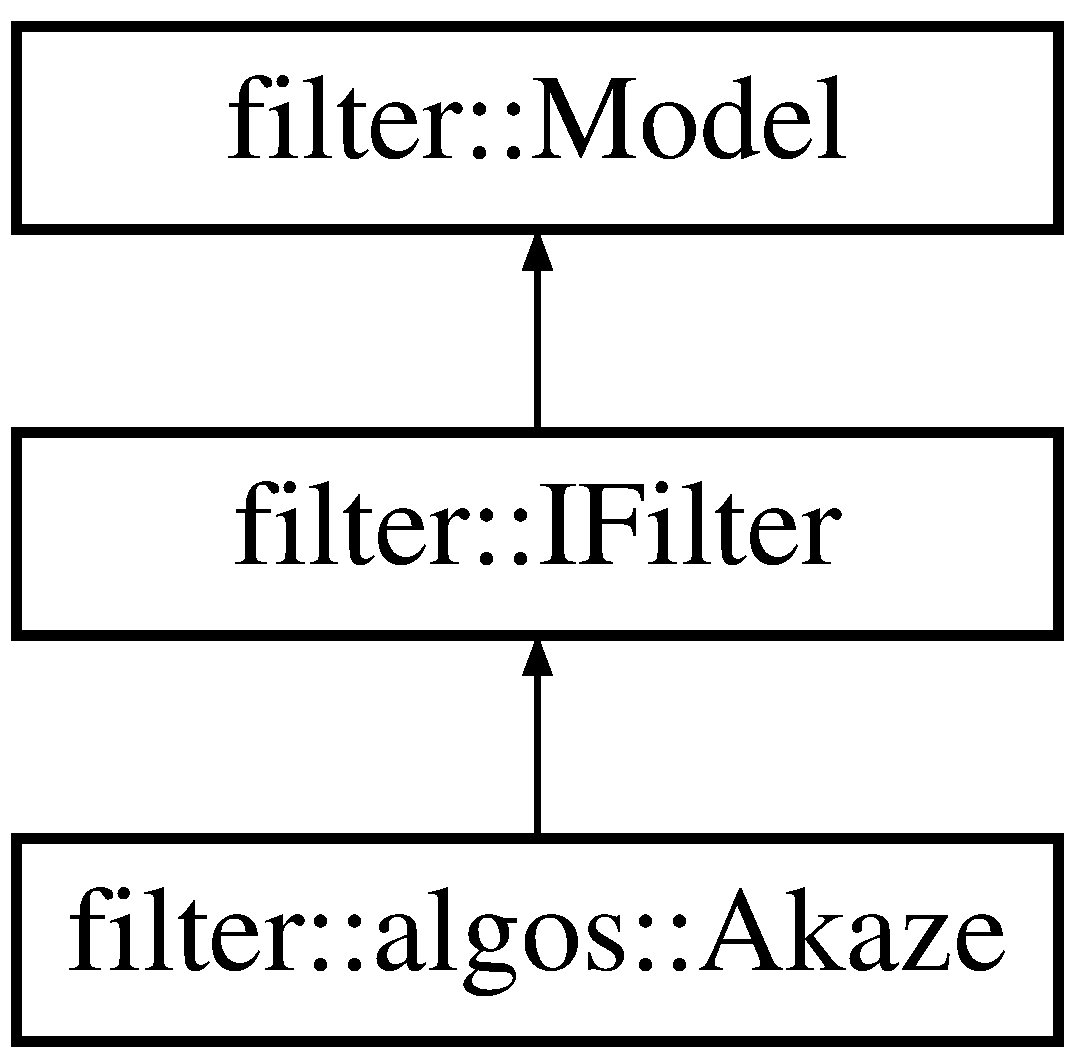
\includegraphics[height=3.000000cm]{d8/d54/classfilter_1_1algos_1_1_akaze}
\end{center}
\end{figure}
\subsection*{Public Types}
\begin{DoxyCompactItemize}
\item 
\mbox{\Hypertarget{classfilter_1_1algos_1_1_akaze_af57f9d7de73fef02601ec7041083c58f}\label{classfilter_1_1algos_1_1_akaze_af57f9d7de73fef02601ec7041083c58f}} 
typedef \hyperlink{class_proxy_functor}{Proxy\+Functor}$<$ \hyperlink{classfilter_1_1algos_1_1_akaze}{Akaze} $>$ {\bfseries \+\_\+proxy\+Functor}
\item 
\mbox{\Hypertarget{classfilter_1_1algos_1_1_akaze_a57b45af3615798e1e01d033f7898b029}\label{classfilter_1_1algos_1_1_akaze_a57b45af3615798e1e01d033f7898b029}} 
typedef \hyperlink{classfilter_1_1algos_1_1_akaze}{Akaze} {\bfseries mytype}
\item 
\mbox{\Hypertarget{classfilter_1_1algos_1_1_akaze_a080f601c3ad170522b9ea2b854bbacf4}\label{classfilter_1_1algos_1_1_akaze_a080f601c3ad170522b9ea2b854bbacf4}} 
typedef float {\bfseries vartype\+\_\+\+\_\+inlier\+\_\+threshold}
\item 
\mbox{\Hypertarget{classfilter_1_1algos_1_1_akaze_aa02421e2cef90028ce64eaa091c5da9c}\label{classfilter_1_1algos_1_1_akaze_aa02421e2cef90028ce64eaa091c5da9c}} 
typedef float {\bfseries vartype\+\_\+\+\_\+nn\+\_\+match\+\_\+ratio}
\end{DoxyCompactItemize}
\subsection*{Public Member Functions}
\begin{DoxyCompactItemize}
\item 
\mbox{\Hypertarget{classfilter_1_1algos_1_1_akaze_a0f01f8c215893b43be88e17add581d4f}\label{classfilter_1_1algos_1_1_akaze_a0f01f8c215893b43be88e17add581d4f}} 
void {\bfseries set\+\_\+inlier\+\_\+threshold\+\_\+from\+\_\+json} (boost\+::property\+\_\+tree\+::ptree \&json\+Class)
\item 
\mbox{\Hypertarget{classfilter_1_1algos_1_1_akaze_a047d4c0ab66d29be98f706a6f3916439}\label{classfilter_1_1algos_1_1_akaze_a047d4c0ab66d29be98f706a6f3916439}} 
void {\bfseries set\+\_\+inlier\+\_\+threshold} (vartype\+\_\+\+\_\+inlier\+\_\+threshold \&\+\_\+\+\_\+inlier\+\_\+threshold)
\item 
\mbox{\Hypertarget{classfilter_1_1algos_1_1_akaze_aaf633d4478bca96d835710ac809e8151}\label{classfilter_1_1algos_1_1_akaze_aaf633d4478bca96d835710ac809e8151}} 
vartype\+\_\+\+\_\+inlier\+\_\+threshold {\bfseries get\+\_\+inlier\+\_\+threshold} ()
\item 
\mbox{\Hypertarget{classfilter_1_1algos_1_1_akaze_a75d02bc78ca516acc7bc5761a415bb68}\label{classfilter_1_1algos_1_1_akaze_a75d02bc78ca516acc7bc5761a415bb68}} 
void {\bfseries copy\+\_\+inlier\+\_\+threshold} (\hyperlink{classfilter_1_1algos_1_1_akaze}{mytype} $\ast$instance)
\item 
\mbox{\Hypertarget{classfilter_1_1algos_1_1_akaze_a4b7c85984e45b759aa63563d8071073c}\label{classfilter_1_1algos_1_1_akaze_a4b7c85984e45b759aa63563d8071073c}} 
void {\bfseries set\+\_\+nn\+\_\+match\+\_\+ratio\+\_\+from\+\_\+json} (boost\+::property\+\_\+tree\+::ptree \&json\+Class)
\item 
\mbox{\Hypertarget{classfilter_1_1algos_1_1_akaze_a19b9239952d34314dc5a977fc581ee01}\label{classfilter_1_1algos_1_1_akaze_a19b9239952d34314dc5a977fc581ee01}} 
void {\bfseries set\+\_\+nn\+\_\+match\+\_\+ratio} (vartype\+\_\+\+\_\+nn\+\_\+match\+\_\+ratio \&\+\_\+\+\_\+nn\+\_\+match\+\_\+ratio)
\item 
\mbox{\Hypertarget{classfilter_1_1algos_1_1_akaze_af3573c50dcc82b6b32a0a4e8ed9db319}\label{classfilter_1_1algos_1_1_akaze_af3573c50dcc82b6b32a0a4e8ed9db319}} 
vartype\+\_\+\+\_\+nn\+\_\+match\+\_\+ratio {\bfseries get\+\_\+nn\+\_\+match\+\_\+ratio} ()
\item 
\mbox{\Hypertarget{classfilter_1_1algos_1_1_akaze_aaa4c674944e460f7585c1e59c89786da}\label{classfilter_1_1algos_1_1_akaze_aaa4c674944e460f7585c1e59c89786da}} 
void {\bfseries copy\+\_\+nn\+\_\+match\+\_\+ratio} (\hyperlink{classfilter_1_1algos_1_1_akaze}{mytype} $\ast$instance)
\item 
virtual std\+::string \hyperlink{classfilter_1_1algos_1_1_akaze_afbbbf680eb0c14ea7e47dbc78169f32b}{result\+As\+String} ()
\begin{DoxyCompactList}\small\item\em Get the result of the processing done by the node. This method will return information only. The actual processing is done by the process() method. \end{DoxyCompactList}\item 
\mbox{\Hypertarget{classfilter_1_1algos_1_1_akaze_a3b23c1d178f81797319dffebbbb77742}\label{classfilter_1_1algos_1_1_akaze_a3b23c1d178f81797319dffebbbb77742}} 
Hipe\+Status {\bfseries process} ()
\end{DoxyCompactItemize}
\subsection*{Public Attributes}
\begin{DoxyCompactItemize}
\item 
float \hyperlink{classfilter_1_1algos_1_1_akaze_aee53a5f3f06ed8c533dc4d421115fe6a}{inlier\+\_\+threshold}
\item 
float \hyperlink{classfilter_1_1algos_1_1_akaze_a114bb2fea06317e4b7c5ba620dd8d3c4}{nn\+\_\+match\+\_\+ratio}
\end{DoxyCompactItemize}
\subsection*{Private Member Functions}
\begin{DoxyCompactItemize}
\item 
\mbox{\Hypertarget{classfilter_1_1algos_1_1_akaze_ae85baf6c729c6e0c9a9ec88cbbb95e7b}\label{classfilter_1_1algos_1_1_akaze_ae85baf6c729c6e0c9a9ec88cbbb95e7b}} 
virtual \hyperlink{classfilter_1_1data_1_1_connex_data_base}{data\+::\+Connex\+Data\+Base} \& {\bfseries get\+Connector} ()
\end{DoxyCompactItemize}
\subsection*{Private Attributes}
\begin{DoxyCompactItemize}
\item 
\mbox{\Hypertarget{classfilter_1_1algos_1_1_akaze_a87f159575ac795211b9af8452bf0a1e5}\label{classfilter_1_1algos_1_1_akaze_a87f159575ac795211b9af8452bf0a1e5}} 
\hyperlink{classfilter_1_1data_1_1_connex_data}{data\+::\+Connex\+Data}$<$ \hyperlink{classfilter_1_1data_1_1_pattern_data}{data\+::\+Pattern\+Data}, \hyperlink{classfilter_1_1data_1_1_image_data}{data\+::\+Image\+Data} $>$ {\bfseries \+\_\+connex\+Data}
\end{DoxyCompactItemize}
\subsection*{Additional Inherited Members}


\subsection{Detailed Description}
\begin{DoxyRefDesc}{Todo}
\item[\hyperlink{todo__todo000001}{Todo}]\end{DoxyRefDesc}
The \hyperlink{classfilter_1_1algos_1_1_akaze}{Akaze} filter is used to find an object on an image in another one using keypoints and the A-\/\+Kaze algorithm. It awaits a Pattern\+Data object as input and will output an image containing the computed matching simimarities contoured. 

\subsection{Member Function Documentation}
\mbox{\Hypertarget{classfilter_1_1algos_1_1_akaze_afbbbf680eb0c14ea7e47dbc78169f32b}\label{classfilter_1_1algos_1_1_akaze_afbbbf680eb0c14ea7e47dbc78169f32b}} 
\index{filter\+::algos\+::\+Akaze@{filter\+::algos\+::\+Akaze}!result\+As\+String@{result\+As\+String}}
\index{result\+As\+String@{result\+As\+String}!filter\+::algos\+::\+Akaze@{filter\+::algos\+::\+Akaze}}
\subsubsection{\texorpdfstring{result\+As\+String()}{resultAsString()}}
{\footnotesize\ttfamily virtual std\+::string filter\+::algos\+::\+Akaze\+::result\+As\+String (\begin{DoxyParamCaption}{ }\end{DoxyParamCaption})\hspace{0.3cm}{\ttfamily [inline]}, {\ttfamily [virtual]}}

\begin{DoxyReturn}{Returns}
A string containing the result of the processing done by the filter. 
\end{DoxyReturn}


Reimplemented from \hyperlink{classfilter_1_1_i_filter_ab99902b060a6d9edc3452a8c9f85e37e}{filter\+::\+I\+Filter}.



\subsection{Member Data Documentation}
\mbox{\Hypertarget{classfilter_1_1algos_1_1_akaze_aee53a5f3f06ed8c533dc4d421115fe6a}\label{classfilter_1_1algos_1_1_akaze_aee53a5f3f06ed8c533dc4d421115fe6a}} 
\index{filter\+::algos\+::\+Akaze@{filter\+::algos\+::\+Akaze}!inlier\+\_\+threshold@{inlier\+\_\+threshold}}
\index{inlier\+\_\+threshold@{inlier\+\_\+threshold}!filter\+::algos\+::\+Akaze@{filter\+::algos\+::\+Akaze}}
\subsubsection{\texorpdfstring{inlier\+\_\+threshold}{inlier\_threshold}}
{\footnotesize\ttfamily filter\+::algos\+::\+Akaze\+::inlier\+\_\+threshold}

The distance threshold used to identify the inliers.\mbox{[}T\+O\+DO\mbox{]} \mbox{\Hypertarget{classfilter_1_1algos_1_1_akaze_a114bb2fea06317e4b7c5ba620dd8d3c4}\label{classfilter_1_1algos_1_1_akaze_a114bb2fea06317e4b7c5ba620dd8d3c4}} 
\index{filter\+::algos\+::\+Akaze@{filter\+::algos\+::\+Akaze}!nn\+\_\+match\+\_\+ratio@{nn\+\_\+match\+\_\+ratio}}
\index{nn\+\_\+match\+\_\+ratio@{nn\+\_\+match\+\_\+ratio}!filter\+::algos\+::\+Akaze@{filter\+::algos\+::\+Akaze}}
\subsubsection{\texorpdfstring{nn\+\_\+match\+\_\+ratio}{nn\_match\_ratio}}
{\footnotesize\ttfamily filter\+::algos\+::\+Akaze\+::nn\+\_\+match\+\_\+ratio}

The ratio used to match the nearests neighbors. 

The documentation for this class was generated from the following files\+:\begin{DoxyCompactItemize}
\item 
header/filter/\+Algos/Akaze.\+h\item 
source/filter/algos/Akaze.\+cpp\end{DoxyCompactItemize}

\hypertarget{classfilter_1_1_algos_1_1_algo_example__1}{}\section{filter\+:\+:Algos\+:\+:Algo\+Example\+\_\+1 Class Reference}
\label{classfilter_1_1_algos_1_1_algo_example__1}\index{filter\+::\+Algos\+::\+Algo\+Example\+\_\+1@{filter\+::\+Algos\+::\+Algo\+Example\+\_\+1}}
Inheritance diagram for filter\+:\+:Algos\+:\+:Algo\+Example\+\_\+1\+:\begin{figure}[H]
\begin{center}
\leavevmode
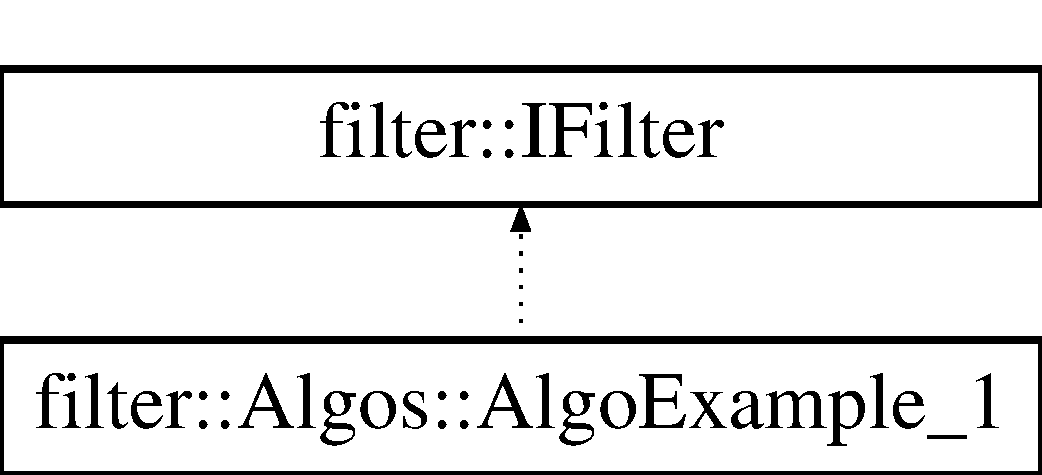
\includegraphics[height=2.000000cm]{d1/d3e/classfilter_1_1_algos_1_1_algo_example__1}
\end{center}
\end{figure}
\subsection*{Additional Inherited Members}


The documentation for this class was generated from the following file\+:\begin{DoxyCompactItemize}
\item 
header/filter/\+Algos/Algo\+Example\+\_\+1.\+h\end{DoxyCompactItemize}

\hypertarget{classfilter_1_1algos_1_1_average_color}{}\section{filter\+:\+:algos\+:\+:Average\+Color Class Reference}
\label{classfilter_1_1algos_1_1_average_color}\index{filter\+::algos\+::\+Average\+Color@{filter\+::algos\+::\+Average\+Color}}


The \hyperlink{classfilter_1_1algos_1_1_average_color}{Average\+Color} filter will compute the average color of an image in R\+GB space. Note that the average color computed will be outputed as an image of 1 pixel.  




{\ttfamily \#include $<$Average\+Color.\+h$>$}

Inheritance diagram for filter\+:\+:algos\+:\+:Average\+Color\+:\begin{figure}[H]
\begin{center}
\leavevmode
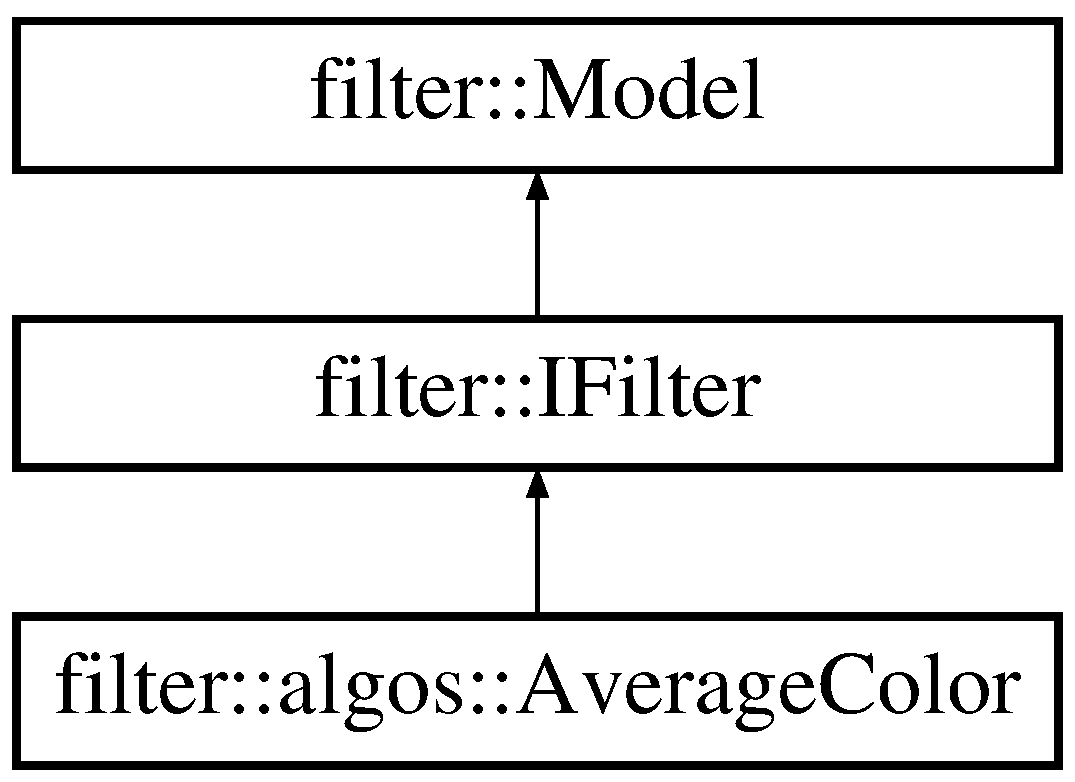
\includegraphics[height=3.000000cm]{d0/d2d/classfilter_1_1algos_1_1_average_color}
\end{center}
\end{figure}
\subsection*{Public Types}
\begin{DoxyCompactItemize}
\item 
\mbox{\Hypertarget{classfilter_1_1algos_1_1_average_color_a6d6bddfbd1497d766e0c16418c2ef5ae}\label{classfilter_1_1algos_1_1_average_color_a6d6bddfbd1497d766e0c16418c2ef5ae}} 
typedef \hyperlink{class_proxy_functor}{Proxy\+Functor}$<$ \hyperlink{classfilter_1_1algos_1_1_average_color}{Average\+Color} $>$ {\bfseries \+\_\+proxy\+Functor}
\item 
\mbox{\Hypertarget{classfilter_1_1algos_1_1_average_color_a8e1c2dc4fd41f7747d7097faf266cf68}\label{classfilter_1_1algos_1_1_average_color_a8e1c2dc4fd41f7747d7097faf266cf68}} 
typedef \hyperlink{classfilter_1_1algos_1_1_average_color}{Average\+Color} {\bfseries mytype}
\item 
\mbox{\Hypertarget{classfilter_1_1algos_1_1_average_color_aea30f21a4e423a96300e69ec91d28caa}\label{classfilter_1_1algos_1_1_average_color_aea30f21a4e423a96300e69ec91d28caa}} 
typedef char {\bfseries vartype\+\_\+\+\_\+unused}
\end{DoxyCompactItemize}
\subsection*{Public Member Functions}
\begin{DoxyCompactItemize}
\item 
\mbox{\Hypertarget{classfilter_1_1algos_1_1_average_color_a77e919dd302fa76438bb6ec5d9c6b397}\label{classfilter_1_1algos_1_1_average_color_a77e919dd302fa76438bb6ec5d9c6b397}} 
void {\bfseries set\+\_\+unused\+\_\+from\+\_\+json} (boost\+::property\+\_\+tree\+::ptree \&json\+Class)
\item 
\mbox{\Hypertarget{classfilter_1_1algos_1_1_average_color_a8adc2c4f61f50fc73a615b50dfb2ddc8}\label{classfilter_1_1algos_1_1_average_color_a8adc2c4f61f50fc73a615b50dfb2ddc8}} 
void {\bfseries set\+\_\+unused} (vartype\+\_\+\+\_\+unused \&\+\_\+\+\_\+unused)
\item 
\mbox{\Hypertarget{classfilter_1_1algos_1_1_average_color_ac1cfc843b2db8dbd6ea10454f432ebaa}\label{classfilter_1_1algos_1_1_average_color_ac1cfc843b2db8dbd6ea10454f432ebaa}} 
vartype\+\_\+\+\_\+unused {\bfseries get\+\_\+unused} ()
\item 
\mbox{\Hypertarget{classfilter_1_1algos_1_1_average_color_a6100f91db703b40f3f686c801e7422cd}\label{classfilter_1_1algos_1_1_average_color_a6100f91db703b40f3f686c801e7422cd}} 
void {\bfseries copy\+\_\+unused} (\hyperlink{classfilter_1_1algos_1_1_average_color}{mytype} $\ast$instance)
\item 
\mbox{\Hypertarget{classfilter_1_1algos_1_1_average_color_ab2a195e0f2fa26df1fa0cad7b3ebed08}\label{classfilter_1_1algos_1_1_average_color_ab2a195e0f2fa26df1fa0cad7b3ebed08}} 
Hipe\+Status {\bfseries process} () override
\end{DoxyCompactItemize}
\subsection*{Public Attributes}
\begin{DoxyCompactItemize}
\item 
\mbox{\Hypertarget{classfilter_1_1algos_1_1_average_color_a92d7fda405ea96e6d2d9aea2fc3ddb87}\label{classfilter_1_1algos_1_1_average_color_a92d7fda405ea96e6d2d9aea2fc3ddb87}} 
char {\bfseries unused}
\end{DoxyCompactItemize}
\subsection*{Private Member Functions}
\begin{DoxyCompactItemize}
\item 
\mbox{\Hypertarget{classfilter_1_1algos_1_1_average_color_ac5e30d428793aba36b2d818b5e941daa}\label{classfilter_1_1algos_1_1_average_color_ac5e30d428793aba36b2d818b5e941daa}} 
virtual \hyperlink{classfilter_1_1data_1_1_connex_data_base}{data\+::\+Connex\+Data\+Base} \& {\bfseries get\+Connector} ()
\end{DoxyCompactItemize}
\subsection*{Private Attributes}
\begin{DoxyCompactItemize}
\item 
\mbox{\Hypertarget{classfilter_1_1algos_1_1_average_color_af480ca1182ca83f8d54da67cc88eb118}\label{classfilter_1_1algos_1_1_average_color_af480ca1182ca83f8d54da67cc88eb118}} 
\hyperlink{classfilter_1_1data_1_1_connex_data}{data\+::\+Connex\+Data}$<$ \hyperlink{classfilter_1_1data_1_1_image_data}{data\+::\+Image\+Data}, \hyperlink{classfilter_1_1data_1_1_image_data}{data\+::\+Image\+Data} $>$ {\bfseries \+\_\+connex\+Data}
\end{DoxyCompactItemize}
\subsection*{Additional Inherited Members}


The documentation for this class was generated from the following file\+:\begin{DoxyCompactItemize}
\item 
header/filter/\+Algos/Average\+Color.\+h\end{DoxyCompactItemize}

\hypertarget{structdt_functor_1_1base}{}\section{dt\+Functor\+:\+:base Struct Reference}
\label{structdt_functor_1_1base}\index{dt\+Functor\+::base@{dt\+Functor\+::base}}
Inheritance diagram for dt\+Functor\+:\+:base\+:\begin{figure}[H]
\begin{center}
\leavevmode
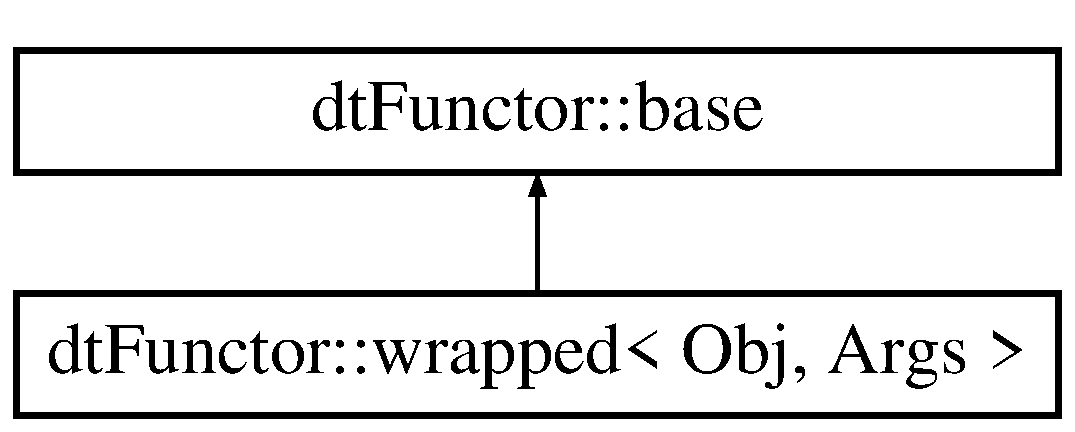
\includegraphics[height=2.000000cm]{d3/df6/structdt_functor_1_1base}
\end{center}
\end{figure}


The documentation for this struct was generated from the following file\+:\begin{DoxyCompactItemize}
\item 
header/filter/tools/functor.\+hpp\end{DoxyCompactItemize}

\hypertarget{class_simple_web_1_1_crypto_1_1_base64}{}\section{Simple\+Web\+:\+:Crypto\+:\+:Base64 Class Reference}
\label{class_simple_web_1_1_crypto_1_1_base64}\index{Simple\+Web\+::\+Crypto\+::\+Base64@{Simple\+Web\+::\+Crypto\+::\+Base64}}
\subsection*{Static Public Member Functions}
\begin{DoxyCompactItemize}
\item 
\mbox{\Hypertarget{class_simple_web_1_1_crypto_1_1_base64_a299572ed812c789fa0a681bd94e282d0}\label{class_simple_web_1_1_crypto_1_1_base64_a299572ed812c789fa0a681bd94e282d0}} 
static std\+::string {\bfseries encode} (const std\+::string \&ascii)
\item 
\mbox{\Hypertarget{class_simple_web_1_1_crypto_1_1_base64_ace7c4c2244925b5068e645cc1d791104}\label{class_simple_web_1_1_crypto_1_1_base64_ace7c4c2244925b5068e645cc1d791104}} 
static std\+::string {\bfseries decode} (const std\+::string \&base64)
\end{DoxyCompactItemize}


The documentation for this class was generated from the following file\+:\begin{DoxyCompactItemize}
\item 
header/http/crypto.\+hpp\end{DoxyCompactItemize}

\hypertarget{class_base_singleton}{}\section{Base\+Singleton Class Reference}
\label{class_base_singleton}\index{Base\+Singleton@{Base\+Singleton}}
Inheritance diagram for Base\+Singleton\+:\begin{figure}[H]
\begin{center}
\leavevmode
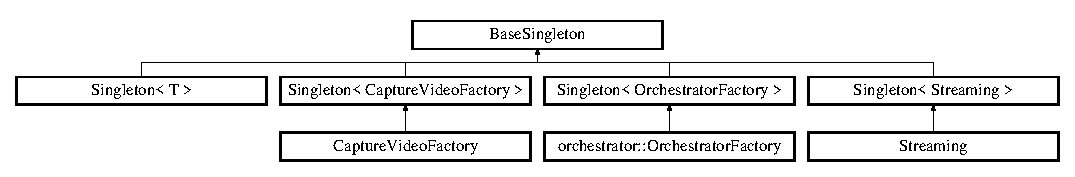
\includegraphics[height=1.926605cm]{d0/d85/class_base_singleton}
\end{center}
\end{figure}


The documentation for this class was generated from the following file\+:\begin{DoxyCompactItemize}
\item 
header/core/Singleton.\+h\end{DoxyCompactItemize}

\hypertarget{classfilter_1_1algos_1_1_bilateral_filter}{}\section{filter\+:\+:algos\+:\+:Bilateral\+Filter Class Reference}
\label{classfilter_1_1algos_1_1_bilateral_filter}\index{filter\+::algos\+::\+Bilateral\+Filter@{filter\+::algos\+::\+Bilateral\+Filter}}


The \hyperlink{classfilter_1_1algos_1_1_bilateral_filter}{Bilateral\+Filter} filter will smooth the image with the bilateral filtering method.  




{\ttfamily \#include $<$Bilateral\+Filter.\+h$>$}

Inheritance diagram for filter\+:\+:algos\+:\+:Bilateral\+Filter\+:\begin{figure}[H]
\begin{center}
\leavevmode
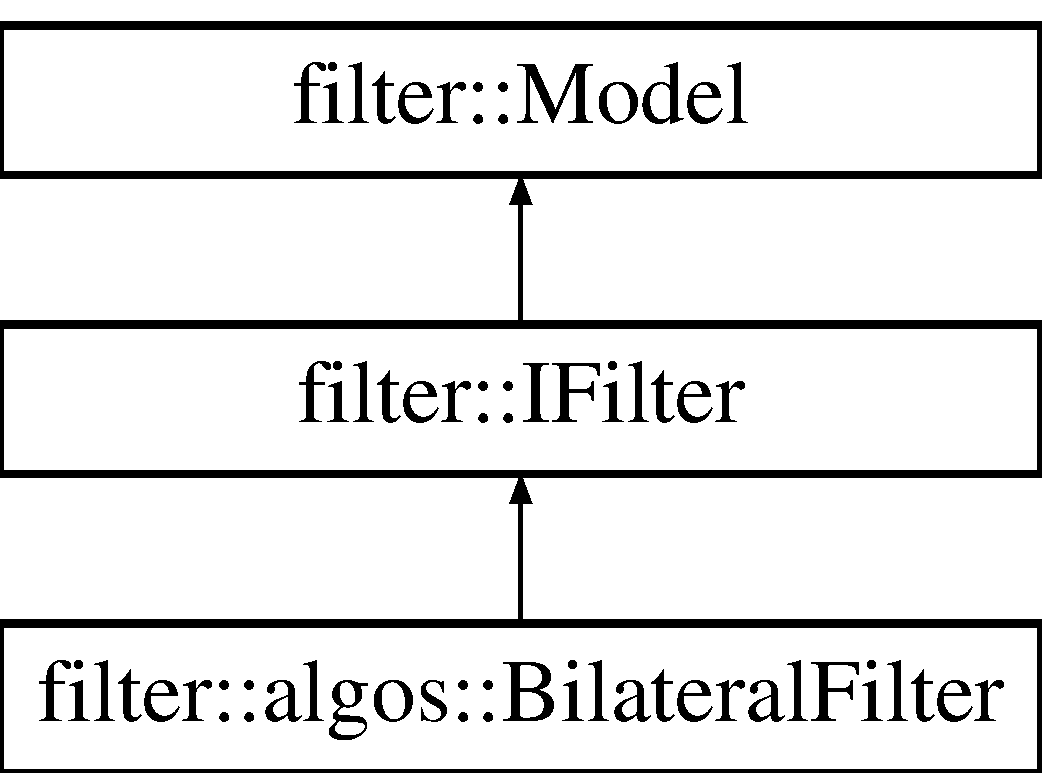
\includegraphics[height=3.000000cm]{d3/dc4/classfilter_1_1algos_1_1_bilateral_filter}
\end{center}
\end{figure}
\subsection*{Public Types}
\begin{DoxyCompactItemize}
\item 
\mbox{\Hypertarget{classfilter_1_1algos_1_1_bilateral_filter_ac0fb679d2ba322f06eeef56fc58db579}\label{classfilter_1_1algos_1_1_bilateral_filter_ac0fb679d2ba322f06eeef56fc58db579}} 
typedef \hyperlink{class_proxy_functor}{Proxy\+Functor}$<$ \hyperlink{classfilter_1_1algos_1_1_bilateral_filter}{Bilateral\+Filter} $>$ {\bfseries \+\_\+proxy\+Functor}
\item 
\mbox{\Hypertarget{classfilter_1_1algos_1_1_bilateral_filter_a092b23218ad9c4a00cf07ab0ad77bb0c}\label{classfilter_1_1algos_1_1_bilateral_filter_a092b23218ad9c4a00cf07ab0ad77bb0c}} 
typedef \hyperlink{classfilter_1_1algos_1_1_bilateral_filter}{Bilateral\+Filter} {\bfseries mytype}
\item 
\mbox{\Hypertarget{classfilter_1_1algos_1_1_bilateral_filter_a6bc6fd02f140606844f758043a64e3d0}\label{classfilter_1_1algos_1_1_bilateral_filter_a6bc6fd02f140606844f758043a64e3d0}} 
typedef int {\bfseries vartype\+\_\+\+\_\+d}
\item 
\mbox{\Hypertarget{classfilter_1_1algos_1_1_bilateral_filter_a1893535ebca02fed8a8534a82c2b8bb1}\label{classfilter_1_1algos_1_1_bilateral_filter_a1893535ebca02fed8a8534a82c2b8bb1}} 
typedef double {\bfseries vartype\+\_\+\+\_\+color}
\item 
\mbox{\Hypertarget{classfilter_1_1algos_1_1_bilateral_filter_a5d71696ab829a205f7e7fa1ebd6dcde3}\label{classfilter_1_1algos_1_1_bilateral_filter_a5d71696ab829a205f7e7fa1ebd6dcde3}} 
typedef double {\bfseries vartype\+\_\+\+\_\+space}
\item 
\mbox{\Hypertarget{classfilter_1_1algos_1_1_bilateral_filter_a83e67b9b3f0cdfa961c162ee54df2a68}\label{classfilter_1_1algos_1_1_bilateral_filter_a83e67b9b3f0cdfa961c162ee54df2a68}} 
typedef int {\bfseries vartype\+\_\+\+\_\+border}
\end{DoxyCompactItemize}
\subsection*{Public Member Functions}
\begin{DoxyCompactItemize}
\item 
\mbox{\Hypertarget{classfilter_1_1algos_1_1_bilateral_filter_aa963e245a6fb9b4f9db2b1b245c3f221}\label{classfilter_1_1algos_1_1_bilateral_filter_aa963e245a6fb9b4f9db2b1b245c3f221}} 
void {\bfseries set\+\_\+d\+\_\+from\+\_\+json} (boost\+::property\+\_\+tree\+::ptree \&json\+Class)
\item 
\mbox{\Hypertarget{classfilter_1_1algos_1_1_bilateral_filter_a0009dbe0037c3b61dd2306cbedd20d11}\label{classfilter_1_1algos_1_1_bilateral_filter_a0009dbe0037c3b61dd2306cbedd20d11}} 
void {\bfseries set\+\_\+d} (vartype\+\_\+\+\_\+d \&\+\_\+\+\_\+d)
\item 
\mbox{\Hypertarget{classfilter_1_1algos_1_1_bilateral_filter_ae3a262210f23e2c7fe44974da55f1e17}\label{classfilter_1_1algos_1_1_bilateral_filter_ae3a262210f23e2c7fe44974da55f1e17}} 
vartype\+\_\+\+\_\+d {\bfseries get\+\_\+d} ()
\item 
\mbox{\Hypertarget{classfilter_1_1algos_1_1_bilateral_filter_a75c966ec263ff507695658afeb96713c}\label{classfilter_1_1algos_1_1_bilateral_filter_a75c966ec263ff507695658afeb96713c}} 
void {\bfseries copy\+\_\+d} (\hyperlink{classfilter_1_1algos_1_1_bilateral_filter}{mytype} $\ast$instance)
\item 
\mbox{\Hypertarget{classfilter_1_1algos_1_1_bilateral_filter_ae971dbc3cb5d874f2e84ea33390d7871}\label{classfilter_1_1algos_1_1_bilateral_filter_ae971dbc3cb5d874f2e84ea33390d7871}} 
void {\bfseries set\+\_\+color\+\_\+from\+\_\+json} (boost\+::property\+\_\+tree\+::ptree \&json\+Class)
\item 
\mbox{\Hypertarget{classfilter_1_1algos_1_1_bilateral_filter_a596c9c41882d5301034c66cae19afc2f}\label{classfilter_1_1algos_1_1_bilateral_filter_a596c9c41882d5301034c66cae19afc2f}} 
void {\bfseries set\+\_\+color} (vartype\+\_\+\+\_\+color \&\+\_\+\+\_\+color)
\item 
\mbox{\Hypertarget{classfilter_1_1algos_1_1_bilateral_filter_a3a6b37a3468e8b03e1ed7db7a2343e34}\label{classfilter_1_1algos_1_1_bilateral_filter_a3a6b37a3468e8b03e1ed7db7a2343e34}} 
vartype\+\_\+\+\_\+color {\bfseries get\+\_\+color} ()
\item 
\mbox{\Hypertarget{classfilter_1_1algos_1_1_bilateral_filter_aafb408f784239f15ef9ca5fcc774e886}\label{classfilter_1_1algos_1_1_bilateral_filter_aafb408f784239f15ef9ca5fcc774e886}} 
void {\bfseries copy\+\_\+color} (\hyperlink{classfilter_1_1algos_1_1_bilateral_filter}{mytype} $\ast$instance)
\item 
\mbox{\Hypertarget{classfilter_1_1algos_1_1_bilateral_filter_a7965c48287c34eb12a00024ef2b0ee56}\label{classfilter_1_1algos_1_1_bilateral_filter_a7965c48287c34eb12a00024ef2b0ee56}} 
void {\bfseries set\+\_\+space\+\_\+from\+\_\+json} (boost\+::property\+\_\+tree\+::ptree \&json\+Class)
\item 
\mbox{\Hypertarget{classfilter_1_1algos_1_1_bilateral_filter_afca21998adf6ea3a2a054276aab54381}\label{classfilter_1_1algos_1_1_bilateral_filter_afca21998adf6ea3a2a054276aab54381}} 
void {\bfseries set\+\_\+space} (vartype\+\_\+\+\_\+space \&\+\_\+\+\_\+space)
\item 
\mbox{\Hypertarget{classfilter_1_1algos_1_1_bilateral_filter_aa47c592a00f4cfc15f97d24c1adc06d5}\label{classfilter_1_1algos_1_1_bilateral_filter_aa47c592a00f4cfc15f97d24c1adc06d5}} 
vartype\+\_\+\+\_\+space {\bfseries get\+\_\+space} ()
\item 
\mbox{\Hypertarget{classfilter_1_1algos_1_1_bilateral_filter_a92084fa723d583f298701041a46e4b9a}\label{classfilter_1_1algos_1_1_bilateral_filter_a92084fa723d583f298701041a46e4b9a}} 
void {\bfseries copy\+\_\+space} (\hyperlink{classfilter_1_1algos_1_1_bilateral_filter}{mytype} $\ast$instance)
\item 
\mbox{\Hypertarget{classfilter_1_1algos_1_1_bilateral_filter_a12f4d5e0f2e32df6a63c19c762914a43}\label{classfilter_1_1algos_1_1_bilateral_filter_a12f4d5e0f2e32df6a63c19c762914a43}} 
void {\bfseries set\+\_\+border\+\_\+from\+\_\+json} (boost\+::property\+\_\+tree\+::ptree \&json\+Class)
\item 
\mbox{\Hypertarget{classfilter_1_1algos_1_1_bilateral_filter_a77d0a143be02bf724978bc1fa382e4c5}\label{classfilter_1_1algos_1_1_bilateral_filter_a77d0a143be02bf724978bc1fa382e4c5}} 
void {\bfseries set\+\_\+border} (vartype\+\_\+\+\_\+border \&\+\_\+\+\_\+border)
\item 
\mbox{\Hypertarget{classfilter_1_1algos_1_1_bilateral_filter_a89cc37eef4ee3c59534f7dbb40850125}\label{classfilter_1_1algos_1_1_bilateral_filter_a89cc37eef4ee3c59534f7dbb40850125}} 
vartype\+\_\+\+\_\+border {\bfseries get\+\_\+border} ()
\item 
\mbox{\Hypertarget{classfilter_1_1algos_1_1_bilateral_filter_a99702ffcc44c830d712803994e233b84}\label{classfilter_1_1algos_1_1_bilateral_filter_a99702ffcc44c830d712803994e233b84}} 
void {\bfseries copy\+\_\+border} (\hyperlink{classfilter_1_1algos_1_1_bilateral_filter}{mytype} $\ast$instance)
\item 
\mbox{\Hypertarget{classfilter_1_1algos_1_1_bilateral_filter_a7c91ab4447b85fb5b0ea0ac6121fc097}\label{classfilter_1_1algos_1_1_bilateral_filter_a7c91ab4447b85fb5b0ea0ac6121fc097}} 
Hipe\+Status {\bfseries process} () override
\end{DoxyCompactItemize}
\subsection*{Public Attributes}
\begin{DoxyCompactItemize}
\item 
int \hyperlink{classfilter_1_1algos_1_1_bilateral_filter_aa5c6a1eb8e86de0868f87b58ac5ca8f5}{d}
\item 
double \hyperlink{classfilter_1_1algos_1_1_bilateral_filter_a3cb2bbf9a7f536d9e706cab30b48f177}{color}
\item 
double \hyperlink{classfilter_1_1algos_1_1_bilateral_filter_a9b408992e14ae094c68c4cd3f706def0}{space}
\item 
int \hyperlink{classfilter_1_1algos_1_1_bilateral_filter_a0254db5121a0c78fcb46d824ab2069d3}{border}
\end{DoxyCompactItemize}
\subsection*{Private Member Functions}
\begin{DoxyCompactItemize}
\item 
\mbox{\Hypertarget{classfilter_1_1algos_1_1_bilateral_filter_ab0ce3ff1bab30775bb2694644912d0c3}\label{classfilter_1_1algos_1_1_bilateral_filter_ab0ce3ff1bab30775bb2694644912d0c3}} 
virtual \hyperlink{classfilter_1_1data_1_1_connex_data_base}{data\+::\+Connex\+Data\+Base} \& {\bfseries get\+Connector} ()
\end{DoxyCompactItemize}
\subsection*{Private Attributes}
\begin{DoxyCompactItemize}
\item 
\mbox{\Hypertarget{classfilter_1_1algos_1_1_bilateral_filter_af6683b48521382d5c269f50f7f6e80ff}\label{classfilter_1_1algos_1_1_bilateral_filter_af6683b48521382d5c269f50f7f6e80ff}} 
\hyperlink{classfilter_1_1data_1_1_connex_data}{data\+::\+Connex\+Data}$<$ \hyperlink{classfilter_1_1data_1_1_image_data}{data\+::\+Image\+Data}, \hyperlink{classfilter_1_1data_1_1_image_data}{data\+::\+Image\+Data} $>$ {\bfseries \+\_\+connex\+Data}
\end{DoxyCompactItemize}
\subsection*{Additional Inherited Members}


\subsection{Detailed Description}
The smoothing method usedwill not alter the edges of the shapes. Mind that the filtering algorithm is performed on the C\+PU, each pass takes a certain amount of time. \begin{DoxySeeAlso}{See also}
cv\+::bilateral\+Filter() 
\end{DoxySeeAlso}


\subsection{Member Data Documentation}
\mbox{\Hypertarget{classfilter_1_1algos_1_1_bilateral_filter_a0254db5121a0c78fcb46d824ab2069d3}\label{classfilter_1_1algos_1_1_bilateral_filter_a0254db5121a0c78fcb46d824ab2069d3}} 
\index{filter\+::algos\+::\+Bilateral\+Filter@{filter\+::algos\+::\+Bilateral\+Filter}!border@{border}}
\index{border@{border}!filter\+::algos\+::\+Bilateral\+Filter@{filter\+::algos\+::\+Bilateral\+Filter}}
\subsubsection{\texorpdfstring{border}{border}}
{\footnotesize\ttfamily filter\+::algos\+::\+Bilateral\+Filter\+::border}

The border mode used to extrapolate pixels outside of the image. \begin{DoxySeeAlso}{See also}
cv\+::\+Border\+Types 
\end{DoxySeeAlso}
\mbox{\Hypertarget{classfilter_1_1algos_1_1_bilateral_filter_a3cb2bbf9a7f536d9e706cab30b48f177}\label{classfilter_1_1algos_1_1_bilateral_filter_a3cb2bbf9a7f536d9e706cab30b48f177}} 
\index{filter\+::algos\+::\+Bilateral\+Filter@{filter\+::algos\+::\+Bilateral\+Filter}!color@{color}}
\index{color@{color}!filter\+::algos\+::\+Bilateral\+Filter@{filter\+::algos\+::\+Bilateral\+Filter}}
\subsubsection{\texorpdfstring{color}{color}}
{\footnotesize\ttfamily filter\+::algos\+::\+Bilateral\+Filter\+::color}

The standard deviation in the color space to apply \mbox{\Hypertarget{classfilter_1_1algos_1_1_bilateral_filter_aa5c6a1eb8e86de0868f87b58ac5ca8f5}\label{classfilter_1_1algos_1_1_bilateral_filter_aa5c6a1eb8e86de0868f87b58ac5ca8f5}} 
\index{filter\+::algos\+::\+Bilateral\+Filter@{filter\+::algos\+::\+Bilateral\+Filter}!d@{d}}
\index{d@{d}!filter\+::algos\+::\+Bilateral\+Filter@{filter\+::algos\+::\+Bilateral\+Filter}}
\subsubsection{\texorpdfstring{d}{d}}
{\footnotesize\ttfamily filter\+::algos\+::\+Bilateral\+Filter\+::d}

The diameter of each pixel neighborhood to use \mbox{\Hypertarget{classfilter_1_1algos_1_1_bilateral_filter_a9b408992e14ae094c68c4cd3f706def0}\label{classfilter_1_1algos_1_1_bilateral_filter_a9b408992e14ae094c68c4cd3f706def0}} 
\index{filter\+::algos\+::\+Bilateral\+Filter@{filter\+::algos\+::\+Bilateral\+Filter}!space@{space}}
\index{space@{space}!filter\+::algos\+::\+Bilateral\+Filter@{filter\+::algos\+::\+Bilateral\+Filter}}
\subsubsection{\texorpdfstring{space}{space}}
{\footnotesize\ttfamily filter\+::algos\+::\+Bilateral\+Filter\+::space}

The standard deviation in the coordinate space (in pixel terms) to apply 

The documentation for this class was generated from the following file\+:\begin{DoxyCompactItemize}
\item 
header/filter/\+Algos/Bilateral\+Filter.\+h\end{DoxyCompactItemize}

\hypertarget{classfilter_1_1algos_1_1_binary}{}\section{filter\+:\+:algos\+:\+:Binary Class Reference}
\label{classfilter_1_1algos_1_1_binary}\index{filter\+::algos\+::\+Binary@{filter\+::algos\+::\+Binary}}


The \hyperlink{classfilter_1_1algos_1_1_binary}{Binary} filter will convert a grayscale image to a black and white one.  




{\ttfamily \#include $<$Binary.\+h$>$}

Inheritance diagram for filter\+:\+:algos\+:\+:Binary\+:\begin{figure}[H]
\begin{center}
\leavevmode
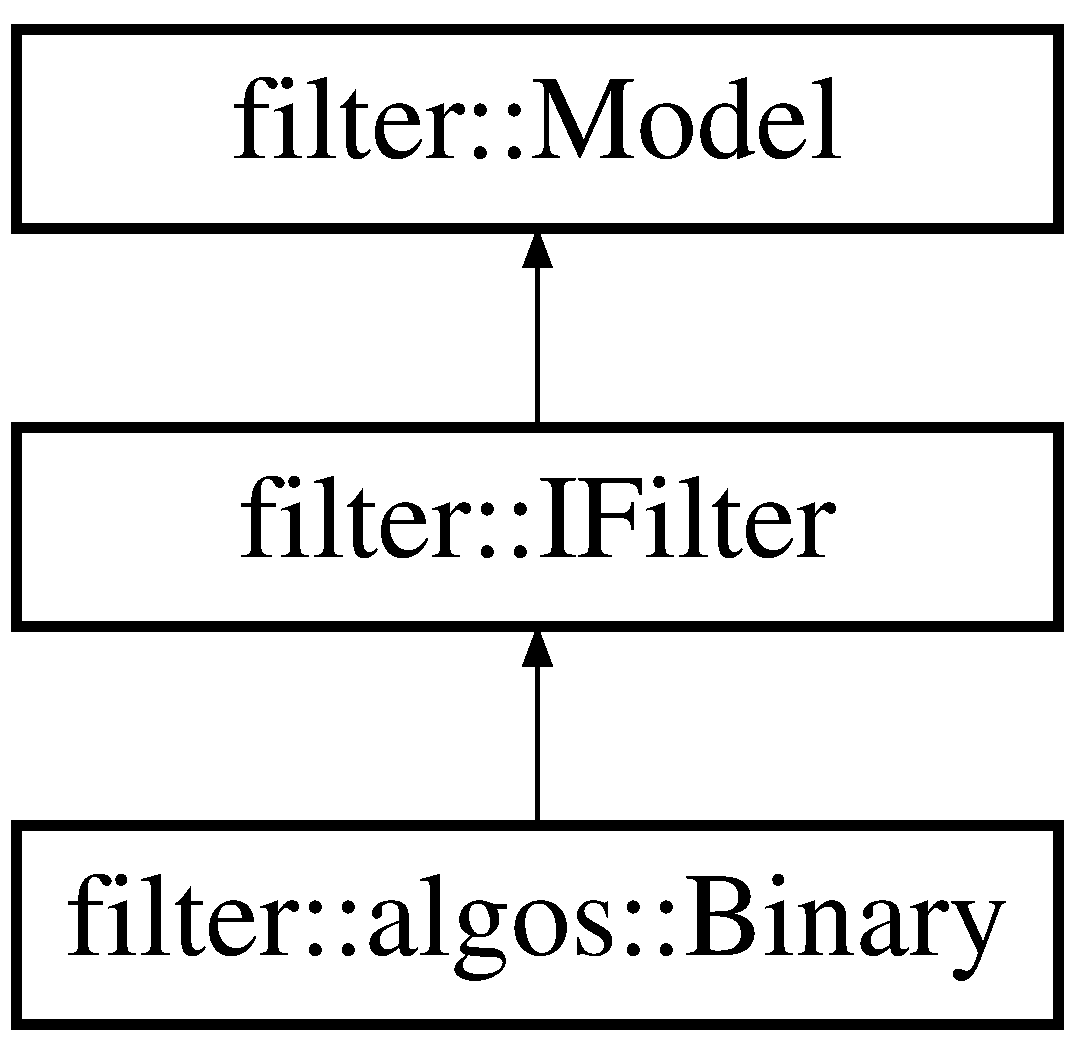
\includegraphics[height=3.000000cm]{d9/dae/classfilter_1_1algos_1_1_binary}
\end{center}
\end{figure}
\subsection*{Public Types}
\begin{DoxyCompactItemize}
\item 
\mbox{\Hypertarget{classfilter_1_1algos_1_1_binary_a48e7bac071c051082cec4d438b9c14c0}\label{classfilter_1_1algos_1_1_binary_a48e7bac071c051082cec4d438b9c14c0}} 
typedef \hyperlink{class_proxy_functor}{Proxy\+Functor}$<$ \hyperlink{classfilter_1_1algos_1_1_binary}{Binary} $>$ {\bfseries \+\_\+proxy\+Functor}
\item 
\mbox{\Hypertarget{classfilter_1_1algos_1_1_binary_a803341d1e8b5a196f8f9023e054558be}\label{classfilter_1_1algos_1_1_binary_a803341d1e8b5a196f8f9023e054558be}} 
typedef \hyperlink{classfilter_1_1algos_1_1_binary}{Binary} {\bfseries mytype}
\item 
\mbox{\Hypertarget{classfilter_1_1algos_1_1_binary_a53eb4696a4ba07aa396ec5e187cafcb4}\label{classfilter_1_1algos_1_1_binary_a53eb4696a4ba07aa396ec5e187cafcb4}} 
typedef std\+::string {\bfseries vartype\+\_\+\+\_\+type}
\item 
\mbox{\Hypertarget{classfilter_1_1algos_1_1_binary_a94cd49147e761efe7af0c2fd7c518776}\label{classfilter_1_1algos_1_1_binary_a94cd49147e761efe7af0c2fd7c518776}} 
typedef double {\bfseries vartype\+\_\+\+\_\+threshold}
\item 
\mbox{\Hypertarget{classfilter_1_1algos_1_1_binary_a4d7b9d5f5efc7ad3c804e3090307042c}\label{classfilter_1_1algos_1_1_binary_a4d7b9d5f5efc7ad3c804e3090307042c}} 
typedef bool {\bfseries vartype\+\_\+\+\_\+otsu}
\item 
\mbox{\Hypertarget{classfilter_1_1algos_1_1_binary_a6b79a74f8c01c2b5c896cb026bb80cac}\label{classfilter_1_1algos_1_1_binary_a6b79a74f8c01c2b5c896cb026bb80cac}} 
typedef double {\bfseries vartype\+\_\+\+\_\+value}
\end{DoxyCompactItemize}
\subsection*{Public Member Functions}
\begin{DoxyCompactItemize}
\item 
\mbox{\Hypertarget{classfilter_1_1algos_1_1_binary_a16019a62863f67b2d63d3727fc05e030}\label{classfilter_1_1algos_1_1_binary_a16019a62863f67b2d63d3727fc05e030}} 
void {\bfseries set\+\_\+type\+\_\+from\+\_\+json} (boost\+::property\+\_\+tree\+::ptree \&json\+Class)
\item 
\mbox{\Hypertarget{classfilter_1_1algos_1_1_binary_a04e237beabe0b8c7805f71686fd5d57c}\label{classfilter_1_1algos_1_1_binary_a04e237beabe0b8c7805f71686fd5d57c}} 
void {\bfseries set\+\_\+type} (vartype\+\_\+\+\_\+type \&\+\_\+\+\_\+type)
\item 
\mbox{\Hypertarget{classfilter_1_1algos_1_1_binary_ac298e2242700e8b36670e7aa14aaa521}\label{classfilter_1_1algos_1_1_binary_ac298e2242700e8b36670e7aa14aaa521}} 
vartype\+\_\+\+\_\+type {\bfseries get\+\_\+type} ()
\item 
\mbox{\Hypertarget{classfilter_1_1algos_1_1_binary_afd69f61c643841bb929fc822f8316135}\label{classfilter_1_1algos_1_1_binary_afd69f61c643841bb929fc822f8316135}} 
void {\bfseries copy\+\_\+type} (\hyperlink{classfilter_1_1algos_1_1_binary}{mytype} $\ast$instance)
\item 
\mbox{\Hypertarget{classfilter_1_1algos_1_1_binary_a6e77978b82ce5ceb2c86f01550351e0c}\label{classfilter_1_1algos_1_1_binary_a6e77978b82ce5ceb2c86f01550351e0c}} 
void {\bfseries set\+\_\+threshold\+\_\+from\+\_\+json} (boost\+::property\+\_\+tree\+::ptree \&json\+Class)
\item 
\mbox{\Hypertarget{classfilter_1_1algos_1_1_binary_af8b5a502f74256e80d03814e9c4e0ca8}\label{classfilter_1_1algos_1_1_binary_af8b5a502f74256e80d03814e9c4e0ca8}} 
void {\bfseries set\+\_\+threshold} (vartype\+\_\+\+\_\+threshold \&\+\_\+\+\_\+threshold)
\item 
\mbox{\Hypertarget{classfilter_1_1algos_1_1_binary_a971aa9d8f12ac3b8dcbe16d40e914c3c}\label{classfilter_1_1algos_1_1_binary_a971aa9d8f12ac3b8dcbe16d40e914c3c}} 
vartype\+\_\+\+\_\+threshold {\bfseries get\+\_\+threshold} ()
\item 
\mbox{\Hypertarget{classfilter_1_1algos_1_1_binary_a7cba60d43da0e82e25d1ae07692aee2c}\label{classfilter_1_1algos_1_1_binary_a7cba60d43da0e82e25d1ae07692aee2c}} 
void {\bfseries copy\+\_\+threshold} (\hyperlink{classfilter_1_1algos_1_1_binary}{mytype} $\ast$instance)
\item 
\mbox{\Hypertarget{classfilter_1_1algos_1_1_binary_a0ceee36e1daeb1356c11f9b27c31e434}\label{classfilter_1_1algos_1_1_binary_a0ceee36e1daeb1356c11f9b27c31e434}} 
void {\bfseries set\+\_\+otsu\+\_\+from\+\_\+json} (boost\+::property\+\_\+tree\+::ptree \&json\+Class)
\item 
\mbox{\Hypertarget{classfilter_1_1algos_1_1_binary_a1b371538af9d35703196032adb2aa4b4}\label{classfilter_1_1algos_1_1_binary_a1b371538af9d35703196032adb2aa4b4}} 
void {\bfseries set\+\_\+otsu} (vartype\+\_\+\+\_\+otsu \&\+\_\+\+\_\+otsu)
\item 
\mbox{\Hypertarget{classfilter_1_1algos_1_1_binary_a39e4676c1948348bc560c6ba35276171}\label{classfilter_1_1algos_1_1_binary_a39e4676c1948348bc560c6ba35276171}} 
vartype\+\_\+\+\_\+otsu {\bfseries get\+\_\+otsu} ()
\item 
\mbox{\Hypertarget{classfilter_1_1algos_1_1_binary_a549489d7fe1afb90c362129aaa43f9f7}\label{classfilter_1_1algos_1_1_binary_a549489d7fe1afb90c362129aaa43f9f7}} 
void {\bfseries copy\+\_\+otsu} (\hyperlink{classfilter_1_1algos_1_1_binary}{mytype} $\ast$instance)
\item 
\mbox{\Hypertarget{classfilter_1_1algos_1_1_binary_a7548655001993c4e0aaab554e7cb178b}\label{classfilter_1_1algos_1_1_binary_a7548655001993c4e0aaab554e7cb178b}} 
void {\bfseries set\+\_\+value\+\_\+from\+\_\+json} (boost\+::property\+\_\+tree\+::ptree \&json\+Class)
\item 
\mbox{\Hypertarget{classfilter_1_1algos_1_1_binary_afe2d4ce88c57f432e780e9e7b3661fd4}\label{classfilter_1_1algos_1_1_binary_afe2d4ce88c57f432e780e9e7b3661fd4}} 
void {\bfseries set\+\_\+value} (vartype\+\_\+\+\_\+value \&\+\_\+\+\_\+value)
\item 
\mbox{\Hypertarget{classfilter_1_1algos_1_1_binary_a1fe90e52279a6de77c7518e14bd568b6}\label{classfilter_1_1algos_1_1_binary_a1fe90e52279a6de77c7518e14bd568b6}} 
vartype\+\_\+\+\_\+value {\bfseries get\+\_\+value} ()
\item 
\mbox{\Hypertarget{classfilter_1_1algos_1_1_binary_aa672c977a7a5e562dbd93b7a7f3aa64d}\label{classfilter_1_1algos_1_1_binary_aa672c977a7a5e562dbd93b7a7f3aa64d}} 
void {\bfseries copy\+\_\+value} (\hyperlink{classfilter_1_1algos_1_1_binary}{mytype} $\ast$instance)
\item 
\mbox{\Hypertarget{classfilter_1_1algos_1_1_binary_a807c847c452e4c1da794afb96d8b78cd}\label{classfilter_1_1algos_1_1_binary_a807c847c452e4c1da794afb96d8b78cd}} 
Hipe\+Status {\bfseries process} () override
\end{DoxyCompactItemize}
\subsection*{Public Attributes}
\begin{DoxyCompactItemize}
\item 
std\+::string \hyperlink{classfilter_1_1algos_1_1_binary_a1f9320375cb787e7f950e5e4721b8022}{type}
\item 
double \hyperlink{classfilter_1_1algos_1_1_binary_ae6e7a193b3a4cfd3cfa96d4102333a06}{threshold}
\item 
bool \hyperlink{classfilter_1_1algos_1_1_binary_a35c09786deafa16fb4053f895c2471b3}{otsu}
\item 
double \hyperlink{classfilter_1_1algos_1_1_binary_a902a7141b452085bb5c1a50b0d0d6bb0}{value}
\end{DoxyCompactItemize}
\subsection*{Private Member Functions}
\begin{DoxyCompactItemize}
\item 
\mbox{\Hypertarget{classfilter_1_1algos_1_1_binary_a07a91319b7715e67bcf83e76b4861a44}\label{classfilter_1_1algos_1_1_binary_a07a91319b7715e67bcf83e76b4861a44}} 
virtual \hyperlink{classfilter_1_1data_1_1_connex_data_base}{data\+::\+Connex\+Data\+Base} \& {\bfseries get\+Connector} ()
\item 
int \hyperlink{classfilter_1_1algos_1_1_binary_a5c2003f1c00b4ae15430ecf42a1cb252}{convert\+Type} (std\+::string \&\hyperlink{classfilter_1_1algos_1_1_binary_a1f9320375cb787e7f950e5e4721b8022}{type})
\begin{DoxyCompactList}\small\item\em Converts a thresholding type inputed as a string to its int value. \end{DoxyCompactList}\end{DoxyCompactItemize}
\subsection*{Private Attributes}
\begin{DoxyCompactItemize}
\item 
\mbox{\Hypertarget{classfilter_1_1algos_1_1_binary_a35da27dc35496b5e3b6d822f1c8d795c}\label{classfilter_1_1algos_1_1_binary_a35da27dc35496b5e3b6d822f1c8d795c}} 
\hyperlink{classfilter_1_1data_1_1_connex_data}{data\+::\+Connex\+Data}$<$ \hyperlink{classfilter_1_1data_1_1_image_data}{data\+::\+Image\+Data}, \hyperlink{classfilter_1_1data_1_1_image_data}{data\+::\+Image\+Data} $>$ {\bfseries \+\_\+connex\+Data}
\end{DoxyCompactItemize}
\subsection*{Additional Inherited Members}


\subsection{Detailed Description}
\begin{DoxySeeAlso}{See also}
cv\+::threshold() 
\end{DoxySeeAlso}


\subsection{Member Function Documentation}
\mbox{\Hypertarget{classfilter_1_1algos_1_1_binary_a5c2003f1c00b4ae15430ecf42a1cb252}\label{classfilter_1_1algos_1_1_binary_a5c2003f1c00b4ae15430ecf42a1cb252}} 
\index{filter\+::algos\+::\+Binary@{filter\+::algos\+::\+Binary}!convert\+Type@{convert\+Type}}
\index{convert\+Type@{convert\+Type}!filter\+::algos\+::\+Binary@{filter\+::algos\+::\+Binary}}
\subsubsection{\texorpdfstring{convert\+Type()}{convertType()}}
{\footnotesize\ttfamily int filter\+::algos\+::\+Binary\+::convert\+Type (\begin{DoxyParamCaption}\item[{std\+::string \&}]{type }\end{DoxyParamCaption})\hspace{0.3cm}{\ttfamily [inline]}, {\ttfamily [private]}}


\begin{DoxyParams}{Parameters}
{\em type} & The type the user inputed. The type must be truncated from its \char`\"{}\+T\+H\+R\+E\+S\+H\+\_\+\char`\"{} prefix \\
\hline
\end{DoxyParams}
\begin{DoxyReturn}{Returns}
Returns the value corresponding to the inputed type 
\end{DoxyReturn}
\begin{DoxySeeAlso}{See also}
cv\+::\+Threshold\+Types 
\end{DoxySeeAlso}


\subsection{Member Data Documentation}
\mbox{\Hypertarget{classfilter_1_1algos_1_1_binary_a35c09786deafa16fb4053f895c2471b3}\label{classfilter_1_1algos_1_1_binary_a35c09786deafa16fb4053f895c2471b3}} 
\index{filter\+::algos\+::\+Binary@{filter\+::algos\+::\+Binary}!otsu@{otsu}}
\index{otsu@{otsu}!filter\+::algos\+::\+Binary@{filter\+::algos\+::\+Binary}}
\subsubsection{\texorpdfstring{otsu}{otsu}}
{\footnotesize\ttfamily filter\+::algos\+::\+Binary\+::otsu}

If set to true, the otsu algorithm will be used insted of the inputed threshold value. The otsu algorithm will dinamycally compute the optimal threshold. Mind that the algorithm only works with 8-\/bit images. \mbox{\Hypertarget{classfilter_1_1algos_1_1_binary_ae6e7a193b3a4cfd3cfa96d4102333a06}\label{classfilter_1_1algos_1_1_binary_ae6e7a193b3a4cfd3cfa96d4102333a06}} 
\index{filter\+::algos\+::\+Binary@{filter\+::algos\+::\+Binary}!threshold@{threshold}}
\index{threshold@{threshold}!filter\+::algos\+::\+Binary@{filter\+::algos\+::\+Binary}}
\subsubsection{\texorpdfstring{threshold}{threshold}}
{\footnotesize\ttfamily filter\+::algos\+::\+Binary\+::threshold}

The threshold value to decide if a pixel will be black, or white \mbox{\Hypertarget{classfilter_1_1algos_1_1_binary_a1f9320375cb787e7f950e5e4721b8022}\label{classfilter_1_1algos_1_1_binary_a1f9320375cb787e7f950e5e4721b8022}} 
\index{filter\+::algos\+::\+Binary@{filter\+::algos\+::\+Binary}!type@{type}}
\index{type@{type}!filter\+::algos\+::\+Binary@{filter\+::algos\+::\+Binary}}
\subsubsection{\texorpdfstring{type}{type}}
{\footnotesize\ttfamily filter\+::algos\+::\+Binary\+::type}

The thresholding type to apply. The type name is truncated from its \char`\"{}\+T\+H\+R\+E\+S\+H\+\_\+\char`\"{} prefix. \begin{DoxySeeAlso}{See also}
cv\+::\+Threshold\+Types 
\end{DoxySeeAlso}
\mbox{\Hypertarget{classfilter_1_1algos_1_1_binary_a902a7141b452085bb5c1a50b0d0d6bb0}\label{classfilter_1_1algos_1_1_binary_a902a7141b452085bb5c1a50b0d0d6bb0}} 
\index{filter\+::algos\+::\+Binary@{filter\+::algos\+::\+Binary}!value@{value}}
\index{value@{value}!filter\+::algos\+::\+Binary@{filter\+::algos\+::\+Binary}}
\subsubsection{\texorpdfstring{value}{value}}
{\footnotesize\ttfamily filter\+::algos\+::\+Binary\+::value}

The value parameter is the value a pixel will take if it passes the threshold test 

The documentation for this class was generated from the following file\+:\begin{DoxyCompactItemize}
\item 
header/filter/\+Algos/Binary.\+h\end{DoxyCompactItemize}

\hypertarget{classfilter_1_1algos_1_1_binary_adaptive}{}\section{filter\+:\+:algos\+:\+:Binary\+Adaptive Class Reference}
\label{classfilter_1_1algos_1_1_binary_adaptive}\index{filter\+::algos\+::\+Binary\+Adaptive@{filter\+::algos\+::\+Binary\+Adaptive}}


The \hyperlink{classfilter_1_1algos_1_1_binary_adaptive}{Binary\+Adaptive} filter will convert a grayscale image to a black and white one.  




{\ttfamily \#include $<$Binary\+Adaptive.\+h$>$}

Inheritance diagram for filter\+:\+:algos\+:\+:Binary\+Adaptive\+:\begin{figure}[H]
\begin{center}
\leavevmode
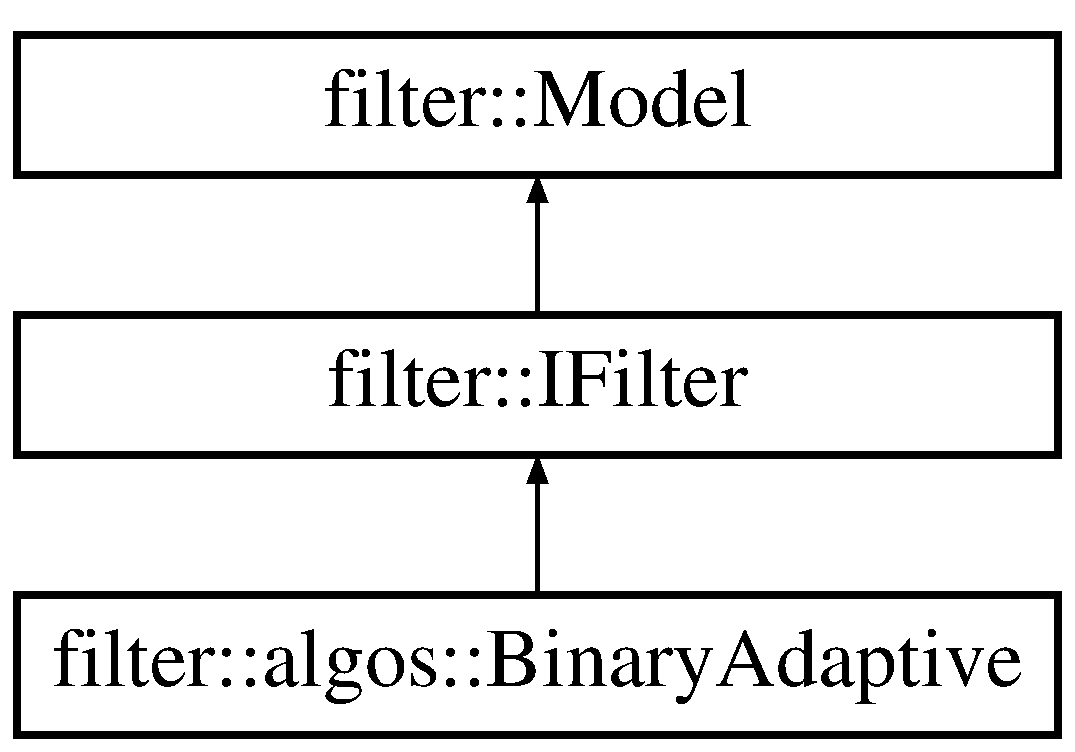
\includegraphics[height=3.000000cm]{d6/d12/classfilter_1_1algos_1_1_binary_adaptive}
\end{center}
\end{figure}
\subsection*{Public Types}
\begin{DoxyCompactItemize}
\item 
\mbox{\Hypertarget{classfilter_1_1algos_1_1_binary_adaptive_aebe508f3835087e12db5ec809fca32ee}\label{classfilter_1_1algos_1_1_binary_adaptive_aebe508f3835087e12db5ec809fca32ee}} 
typedef \hyperlink{class_proxy_functor}{Proxy\+Functor}$<$ \hyperlink{classfilter_1_1algos_1_1_binary_adaptive}{Binary\+Adaptive} $>$ {\bfseries \+\_\+proxy\+Functor}
\item 
\mbox{\Hypertarget{classfilter_1_1algos_1_1_binary_adaptive_a289438d25158f006118906c0498a5a41}\label{classfilter_1_1algos_1_1_binary_adaptive_a289438d25158f006118906c0498a5a41}} 
typedef \hyperlink{classfilter_1_1algos_1_1_binary_adaptive}{Binary\+Adaptive} {\bfseries mytype}
\item 
\mbox{\Hypertarget{classfilter_1_1algos_1_1_binary_adaptive_a9e7c7117788e8bf76a2f65ca7fd0e516}\label{classfilter_1_1algos_1_1_binary_adaptive_a9e7c7117788e8bf76a2f65ca7fd0e516}} 
typedef std\+::string {\bfseries vartype\+\_\+\+\_\+type}
\item 
\mbox{\Hypertarget{classfilter_1_1algos_1_1_binary_adaptive_a1d8556ac91145da50fb57a87aaad732f}\label{classfilter_1_1algos_1_1_binary_adaptive_a1d8556ac91145da50fb57a87aaad732f}} 
typedef std\+::string {\bfseries vartype\+\_\+\+\_\+method}
\item 
\mbox{\Hypertarget{classfilter_1_1algos_1_1_binary_adaptive_a3175af4559a3708edf39baa929acb3c3}\label{classfilter_1_1algos_1_1_binary_adaptive_a3175af4559a3708edf39baa929acb3c3}} 
typedef int {\bfseries vartype\+\_\+\+\_\+block}
\item 
\mbox{\Hypertarget{classfilter_1_1algos_1_1_binary_adaptive_ac3980041c1ea2adb95093309740295b5}\label{classfilter_1_1algos_1_1_binary_adaptive_ac3980041c1ea2adb95093309740295b5}} 
typedef double {\bfseries vartype\+\_\+\+\_\+value}
\item 
\mbox{\Hypertarget{classfilter_1_1algos_1_1_binary_adaptive_a50633e873f900f1399952076d0ddd5b5}\label{classfilter_1_1algos_1_1_binary_adaptive_a50633e873f900f1399952076d0ddd5b5}} 
typedef double {\bfseries vartype\+\_\+\+\_\+c}
\end{DoxyCompactItemize}
\subsection*{Public Member Functions}
\begin{DoxyCompactItemize}
\item 
\mbox{\Hypertarget{classfilter_1_1algos_1_1_binary_adaptive_a7f3d6541fbdb9692fd414159355abd2a}\label{classfilter_1_1algos_1_1_binary_adaptive_a7f3d6541fbdb9692fd414159355abd2a}} 
void {\bfseries set\+\_\+type\+\_\+from\+\_\+json} (boost\+::property\+\_\+tree\+::ptree \&json\+Class)
\item 
\mbox{\Hypertarget{classfilter_1_1algos_1_1_binary_adaptive_a87bd21febf5b3a8ad4ad47cfc33a5b37}\label{classfilter_1_1algos_1_1_binary_adaptive_a87bd21febf5b3a8ad4ad47cfc33a5b37}} 
void {\bfseries set\+\_\+type} (vartype\+\_\+\+\_\+type \&\+\_\+\+\_\+type)
\item 
\mbox{\Hypertarget{classfilter_1_1algos_1_1_binary_adaptive_ac4c63a470a9562c1a3b15bcbff3aab73}\label{classfilter_1_1algos_1_1_binary_adaptive_ac4c63a470a9562c1a3b15bcbff3aab73}} 
vartype\+\_\+\+\_\+type {\bfseries get\+\_\+type} ()
\item 
\mbox{\Hypertarget{classfilter_1_1algos_1_1_binary_adaptive_a1d8ee180da87f5223a419cd06b261c5e}\label{classfilter_1_1algos_1_1_binary_adaptive_a1d8ee180da87f5223a419cd06b261c5e}} 
void {\bfseries copy\+\_\+type} (\hyperlink{classfilter_1_1algos_1_1_binary_adaptive}{mytype} $\ast$instance)
\item 
\mbox{\Hypertarget{classfilter_1_1algos_1_1_binary_adaptive_aaf708f9c26f801d9328b2c6eab8a8eac}\label{classfilter_1_1algos_1_1_binary_adaptive_aaf708f9c26f801d9328b2c6eab8a8eac}} 
void {\bfseries set\+\_\+method\+\_\+from\+\_\+json} (boost\+::property\+\_\+tree\+::ptree \&json\+Class)
\item 
\mbox{\Hypertarget{classfilter_1_1algos_1_1_binary_adaptive_aaf2c08ccd0d4fb73cf25fe75bfda5563}\label{classfilter_1_1algos_1_1_binary_adaptive_aaf2c08ccd0d4fb73cf25fe75bfda5563}} 
void {\bfseries set\+\_\+method} (vartype\+\_\+\+\_\+method \&\+\_\+\+\_\+method)
\item 
\mbox{\Hypertarget{classfilter_1_1algos_1_1_binary_adaptive_a8bcee7536f8977938c19556eaac5c994}\label{classfilter_1_1algos_1_1_binary_adaptive_a8bcee7536f8977938c19556eaac5c994}} 
vartype\+\_\+\+\_\+method {\bfseries get\+\_\+method} ()
\item 
\mbox{\Hypertarget{classfilter_1_1algos_1_1_binary_adaptive_a944fee61b03bec23221203f3280b89bf}\label{classfilter_1_1algos_1_1_binary_adaptive_a944fee61b03bec23221203f3280b89bf}} 
void {\bfseries copy\+\_\+method} (\hyperlink{classfilter_1_1algos_1_1_binary_adaptive}{mytype} $\ast$instance)
\item 
\mbox{\Hypertarget{classfilter_1_1algos_1_1_binary_adaptive_a4c8005c27121340d846d3731bbe3e5d5}\label{classfilter_1_1algos_1_1_binary_adaptive_a4c8005c27121340d846d3731bbe3e5d5}} 
void {\bfseries set\+\_\+block\+\_\+from\+\_\+json} (boost\+::property\+\_\+tree\+::ptree \&json\+Class)
\item 
\mbox{\Hypertarget{classfilter_1_1algos_1_1_binary_adaptive_a91706d3d3696dc83a5873e05271224ee}\label{classfilter_1_1algos_1_1_binary_adaptive_a91706d3d3696dc83a5873e05271224ee}} 
void {\bfseries set\+\_\+block} (vartype\+\_\+\+\_\+block \&\+\_\+\+\_\+block)
\item 
\mbox{\Hypertarget{classfilter_1_1algos_1_1_binary_adaptive_a351cb7df5ae8b4a704b310f7580d5309}\label{classfilter_1_1algos_1_1_binary_adaptive_a351cb7df5ae8b4a704b310f7580d5309}} 
vartype\+\_\+\+\_\+block {\bfseries get\+\_\+block} ()
\item 
\mbox{\Hypertarget{classfilter_1_1algos_1_1_binary_adaptive_a749bf777c5d9804becf9964375e61733}\label{classfilter_1_1algos_1_1_binary_adaptive_a749bf777c5d9804becf9964375e61733}} 
void {\bfseries copy\+\_\+block} (\hyperlink{classfilter_1_1algos_1_1_binary_adaptive}{mytype} $\ast$instance)
\item 
\mbox{\Hypertarget{classfilter_1_1algos_1_1_binary_adaptive_a3b6091314dfc7c9e6d54ec428749d2c9}\label{classfilter_1_1algos_1_1_binary_adaptive_a3b6091314dfc7c9e6d54ec428749d2c9}} 
void {\bfseries set\+\_\+value\+\_\+from\+\_\+json} (boost\+::property\+\_\+tree\+::ptree \&json\+Class)
\item 
\mbox{\Hypertarget{classfilter_1_1algos_1_1_binary_adaptive_a3fe7e1d537b24d7f9b9c187451892deb}\label{classfilter_1_1algos_1_1_binary_adaptive_a3fe7e1d537b24d7f9b9c187451892deb}} 
void {\bfseries set\+\_\+value} (vartype\+\_\+\+\_\+value \&\+\_\+\+\_\+value)
\item 
\mbox{\Hypertarget{classfilter_1_1algos_1_1_binary_adaptive_aab420592e5dd56029eaee8cb569282d0}\label{classfilter_1_1algos_1_1_binary_adaptive_aab420592e5dd56029eaee8cb569282d0}} 
vartype\+\_\+\+\_\+value {\bfseries get\+\_\+value} ()
\item 
\mbox{\Hypertarget{classfilter_1_1algos_1_1_binary_adaptive_ac67c6bf1667e3fb68fb14df1629de378}\label{classfilter_1_1algos_1_1_binary_adaptive_ac67c6bf1667e3fb68fb14df1629de378}} 
void {\bfseries copy\+\_\+value} (\hyperlink{classfilter_1_1algos_1_1_binary_adaptive}{mytype} $\ast$instance)
\item 
\mbox{\Hypertarget{classfilter_1_1algos_1_1_binary_adaptive_a0c82b3e231c3f5e4d820d408bde2d0c4}\label{classfilter_1_1algos_1_1_binary_adaptive_a0c82b3e231c3f5e4d820d408bde2d0c4}} 
void {\bfseries set\+\_\+c\+\_\+from\+\_\+json} (boost\+::property\+\_\+tree\+::ptree \&json\+Class)
\item 
\mbox{\Hypertarget{classfilter_1_1algos_1_1_binary_adaptive_adaf84bcdf3380d958f1236e98cc85bcd}\label{classfilter_1_1algos_1_1_binary_adaptive_adaf84bcdf3380d958f1236e98cc85bcd}} 
void {\bfseries set\+\_\+c} (vartype\+\_\+\+\_\+c \&\+\_\+\+\_\+c)
\item 
\mbox{\Hypertarget{classfilter_1_1algos_1_1_binary_adaptive_a34b11512baec0cfffc7b5b679acd08d9}\label{classfilter_1_1algos_1_1_binary_adaptive_a34b11512baec0cfffc7b5b679acd08d9}} 
vartype\+\_\+\+\_\+c {\bfseries get\+\_\+c} ()
\item 
\mbox{\Hypertarget{classfilter_1_1algos_1_1_binary_adaptive_acd8a25c3670e064aba1fed85d76d2e80}\label{classfilter_1_1algos_1_1_binary_adaptive_acd8a25c3670e064aba1fed85d76d2e80}} 
void {\bfseries copy\+\_\+c} (\hyperlink{classfilter_1_1algos_1_1_binary_adaptive}{mytype} $\ast$instance)
\item 
\mbox{\Hypertarget{classfilter_1_1algos_1_1_binary_adaptive_a9026458211dd46de236a1addcd0903be}\label{classfilter_1_1algos_1_1_binary_adaptive_a9026458211dd46de236a1addcd0903be}} 
Hipe\+Status {\bfseries process} () override
\end{DoxyCompactItemize}
\subsection*{Public Attributes}
\begin{DoxyCompactItemize}
\item 
std\+::string \hyperlink{classfilter_1_1algos_1_1_binary_adaptive_a8256a8c340fbc64eaf1fa4232d910435}{type}
\item 
std\+::string \hyperlink{classfilter_1_1algos_1_1_binary_adaptive_a67df7719f9d5ace093fb1b70455f7a4f}{method}
\item 
int \hyperlink{classfilter_1_1algos_1_1_binary_adaptive_ad36a47f5f1a5cc2b78f17ab842e31487}{block}
\item 
double \hyperlink{classfilter_1_1algos_1_1_binary_adaptive_ae61f0f9c3449d7025d88508445005cc7}{value}
\item 
double \hyperlink{classfilter_1_1algos_1_1_binary_adaptive_acce86b4d7f1370bc36cd283dcc26970c}{c}
\end{DoxyCompactItemize}
\subsection*{Private Member Functions}
\begin{DoxyCompactItemize}
\item 
\mbox{\Hypertarget{classfilter_1_1algos_1_1_binary_adaptive_a1fe10a09e339e48dc98df4d0642cb816}\label{classfilter_1_1algos_1_1_binary_adaptive_a1fe10a09e339e48dc98df4d0642cb816}} 
virtual \hyperlink{classfilter_1_1data_1_1_connex_data_base}{data\+::\+Connex\+Data\+Base} \& {\bfseries get\+Connector} ()
\item 
int \hyperlink{classfilter_1_1algos_1_1_binary_adaptive_a06e3ad587fb9e958e19ded273c70e4e1}{convert\+Type} (std\+::string \&\hyperlink{classfilter_1_1algos_1_1_binary_adaptive_a8256a8c340fbc64eaf1fa4232d910435}{type})
\begin{DoxyCompactList}\small\item\em Converts a thresholding type inputed as a string to its int value. \end{DoxyCompactList}\item 
int \hyperlink{classfilter_1_1algos_1_1_binary_adaptive_a2cca79f85248dff026bf39d1940a60d6}{convert\+Adaptive} (std\+::string \&\hyperlink{classfilter_1_1algos_1_1_binary_adaptive_a67df7719f9d5ace093fb1b70455f7a4f}{method})
\begin{DoxyCompactList}\small\item\em Converts a thresholding method inputed as a string to its int value. \end{DoxyCompactList}\end{DoxyCompactItemize}
\subsection*{Private Attributes}
\begin{DoxyCompactItemize}
\item 
\mbox{\Hypertarget{classfilter_1_1algos_1_1_binary_adaptive_ad56ec711d50924b0f401a86550767afb}\label{classfilter_1_1algos_1_1_binary_adaptive_ad56ec711d50924b0f401a86550767afb}} 
\hyperlink{classfilter_1_1data_1_1_connex_data}{data\+::\+Connex\+Data}$<$ \hyperlink{classfilter_1_1data_1_1_image_data}{data\+::\+Image\+Data}, \hyperlink{classfilter_1_1data_1_1_image_data}{data\+::\+Image\+Data} $>$ {\bfseries \+\_\+connex\+Data}
\end{DoxyCompactItemize}
\subsection*{Additional Inherited Members}


\subsection{Detailed Description}
Unlike the \hyperlink{classfilter_1_1algos_1_1_binary}{Binary} filter, the \hyperlink{classfilter_1_1algos_1_1_binary_adaptive}{Binary\+Adaptive} filter will divide the image in sub regions and dinamycally compute the optimal threshold value for each of them. It is useful for images with variations in illumination. \begin{DoxySeeAlso}{See also}
cv\+::adaptive\+Threshold() 
\end{DoxySeeAlso}


\subsection{Member Function Documentation}
\mbox{\Hypertarget{classfilter_1_1algos_1_1_binary_adaptive_a2cca79f85248dff026bf39d1940a60d6}\label{classfilter_1_1algos_1_1_binary_adaptive_a2cca79f85248dff026bf39d1940a60d6}} 
\index{filter\+::algos\+::\+Binary\+Adaptive@{filter\+::algos\+::\+Binary\+Adaptive}!convert\+Adaptive@{convert\+Adaptive}}
\index{convert\+Adaptive@{convert\+Adaptive}!filter\+::algos\+::\+Binary\+Adaptive@{filter\+::algos\+::\+Binary\+Adaptive}}
\subsubsection{\texorpdfstring{convert\+Adaptive()}{convertAdaptive()}}
{\footnotesize\ttfamily int filter\+::algos\+::\+Binary\+Adaptive\+::convert\+Adaptive (\begin{DoxyParamCaption}\item[{std\+::string \&}]{method }\end{DoxyParamCaption})\hspace{0.3cm}{\ttfamily [inline]}, {\ttfamily [private]}}


\begin{DoxyParams}{Parameters}
{\em method} & The type the user inputed. The type must be truncated from its \char`\"{}\+A\+D\+A\+P\+T\+I\+V\+E\+\_\+\+T\+H\+R\+E\+S\+H\+\_\+\char`\"{} prefix \\
\hline
\end{DoxyParams}
\begin{DoxyReturn}{Returns}
Returns the value corresponding to the inputed type. 
\end{DoxyReturn}
\begin{DoxySeeAlso}{See also}
cv\+::\+Adaptive\+Threshold\+Types 
\end{DoxySeeAlso}
\mbox{\Hypertarget{classfilter_1_1algos_1_1_binary_adaptive_a06e3ad587fb9e958e19ded273c70e4e1}\label{classfilter_1_1algos_1_1_binary_adaptive_a06e3ad587fb9e958e19ded273c70e4e1}} 
\index{filter\+::algos\+::\+Binary\+Adaptive@{filter\+::algos\+::\+Binary\+Adaptive}!convert\+Type@{convert\+Type}}
\index{convert\+Type@{convert\+Type}!filter\+::algos\+::\+Binary\+Adaptive@{filter\+::algos\+::\+Binary\+Adaptive}}
\subsubsection{\texorpdfstring{convert\+Type()}{convertType()}}
{\footnotesize\ttfamily int filter\+::algos\+::\+Binary\+Adaptive\+::convert\+Type (\begin{DoxyParamCaption}\item[{std\+::string \&}]{type }\end{DoxyParamCaption})\hspace{0.3cm}{\ttfamily [inline]}, {\ttfamily [private]}}


\begin{DoxyParams}{Parameters}
{\em type} & The type the user inputed. The type must be truncated from its \char`\"{}\+T\+H\+R\+E\+S\+H\+\_\+\char`\"{} prefix \\
\hline
\end{DoxyParams}
\begin{DoxyReturn}{Returns}
Returns the value corresponding to the inputed type 
\end{DoxyReturn}
\begin{DoxySeeAlso}{See also}
cv\+::\+Threshold\+Types 
\end{DoxySeeAlso}


\subsection{Member Data Documentation}
\mbox{\Hypertarget{classfilter_1_1algos_1_1_binary_adaptive_ad36a47f5f1a5cc2b78f17ab842e31487}\label{classfilter_1_1algos_1_1_binary_adaptive_ad36a47f5f1a5cc2b78f17ab842e31487}} 
\index{filter\+::algos\+::\+Binary\+Adaptive@{filter\+::algos\+::\+Binary\+Adaptive}!block@{block}}
\index{block@{block}!filter\+::algos\+::\+Binary\+Adaptive@{filter\+::algos\+::\+Binary\+Adaptive}}
\subsubsection{\texorpdfstring{block}{block}}
{\footnotesize\ttfamily filter\+::algos\+::\+Binary\+Adaptive\+::block}

The kernel\textquotesingle{}s size to use to compute the threshold. It is the number of neighbouring pixels to analyze. \mbox{\Hypertarget{classfilter_1_1algos_1_1_binary_adaptive_acce86b4d7f1370bc36cd283dcc26970c}\label{classfilter_1_1algos_1_1_binary_adaptive_acce86b4d7f1370bc36cd283dcc26970c}} 
\index{filter\+::algos\+::\+Binary\+Adaptive@{filter\+::algos\+::\+Binary\+Adaptive}!c@{c}}
\index{c@{c}!filter\+::algos\+::\+Binary\+Adaptive@{filter\+::algos\+::\+Binary\+Adaptive}}
\subsubsection{\texorpdfstring{c}{c}}
{\footnotesize\ttfamily filter\+::algos\+::\+Binary\+Adaptive\+::c}

A constant to substract to the computed mean or weighted mean. \mbox{[}T\+O\+DO\mbox{]} \mbox{\Hypertarget{classfilter_1_1algos_1_1_binary_adaptive_a67df7719f9d5ace093fb1b70455f7a4f}\label{classfilter_1_1algos_1_1_binary_adaptive_a67df7719f9d5ace093fb1b70455f7a4f}} 
\index{filter\+::algos\+::\+Binary\+Adaptive@{filter\+::algos\+::\+Binary\+Adaptive}!method@{method}}
\index{method@{method}!filter\+::algos\+::\+Binary\+Adaptive@{filter\+::algos\+::\+Binary\+Adaptive}}
\subsubsection{\texorpdfstring{method}{method}}
{\footnotesize\ttfamily filter\+::algos\+::\+Binary\+Adaptive\+::method}

The adaptive thresholding algorithm to use. \begin{DoxySeeAlso}{See also}
cv\+::\+Adaptive\+Threshold\+Types 
\end{DoxySeeAlso}
\mbox{\Hypertarget{classfilter_1_1algos_1_1_binary_adaptive_a8256a8c340fbc64eaf1fa4232d910435}\label{classfilter_1_1algos_1_1_binary_adaptive_a8256a8c340fbc64eaf1fa4232d910435}} 
\index{filter\+::algos\+::\+Binary\+Adaptive@{filter\+::algos\+::\+Binary\+Adaptive}!type@{type}}
\index{type@{type}!filter\+::algos\+::\+Binary\+Adaptive@{filter\+::algos\+::\+Binary\+Adaptive}}
\subsubsection{\texorpdfstring{type}{type}}
{\footnotesize\ttfamily filter\+::algos\+::\+Binary\+Adaptive\+::type}

The thresholding method to apply. \begin{DoxySeeAlso}{See also}
cv\+::\+Threshold\+Types 
\end{DoxySeeAlso}
\mbox{\Hypertarget{classfilter_1_1algos_1_1_binary_adaptive_ae61f0f9c3449d7025d88508445005cc7}\label{classfilter_1_1algos_1_1_binary_adaptive_ae61f0f9c3449d7025d88508445005cc7}} 
\index{filter\+::algos\+::\+Binary\+Adaptive@{filter\+::algos\+::\+Binary\+Adaptive}!value@{value}}
\index{value@{value}!filter\+::algos\+::\+Binary\+Adaptive@{filter\+::algos\+::\+Binary\+Adaptive}}
\subsubsection{\texorpdfstring{value}{value}}
{\footnotesize\ttfamily filter\+::algos\+::\+Binary\+Adaptive\+::value}

The value parameter is the value a pixel will take if it passes the threshold test. 

The documentation for this class was generated from the following file\+:\begin{DoxyCompactItemize}
\item 
header/filter/\+Algos/Binary\+Adaptive.\+h\end{DoxyCompactItemize}

\hypertarget{classfilter_1_1algos_1_1_blur}{}\section{filter\+:\+:algos\+:\+:Blur Class Reference}
\label{classfilter_1_1algos_1_1_blur}\index{filter\+::algos\+::\+Blur@{filter\+::algos\+::\+Blur}}


The blur filter will blur an image.  




{\ttfamily \#include $<$Blur.\+h$>$}

Inheritance diagram for filter\+:\+:algos\+:\+:Blur\+:\begin{figure}[H]
\begin{center}
\leavevmode
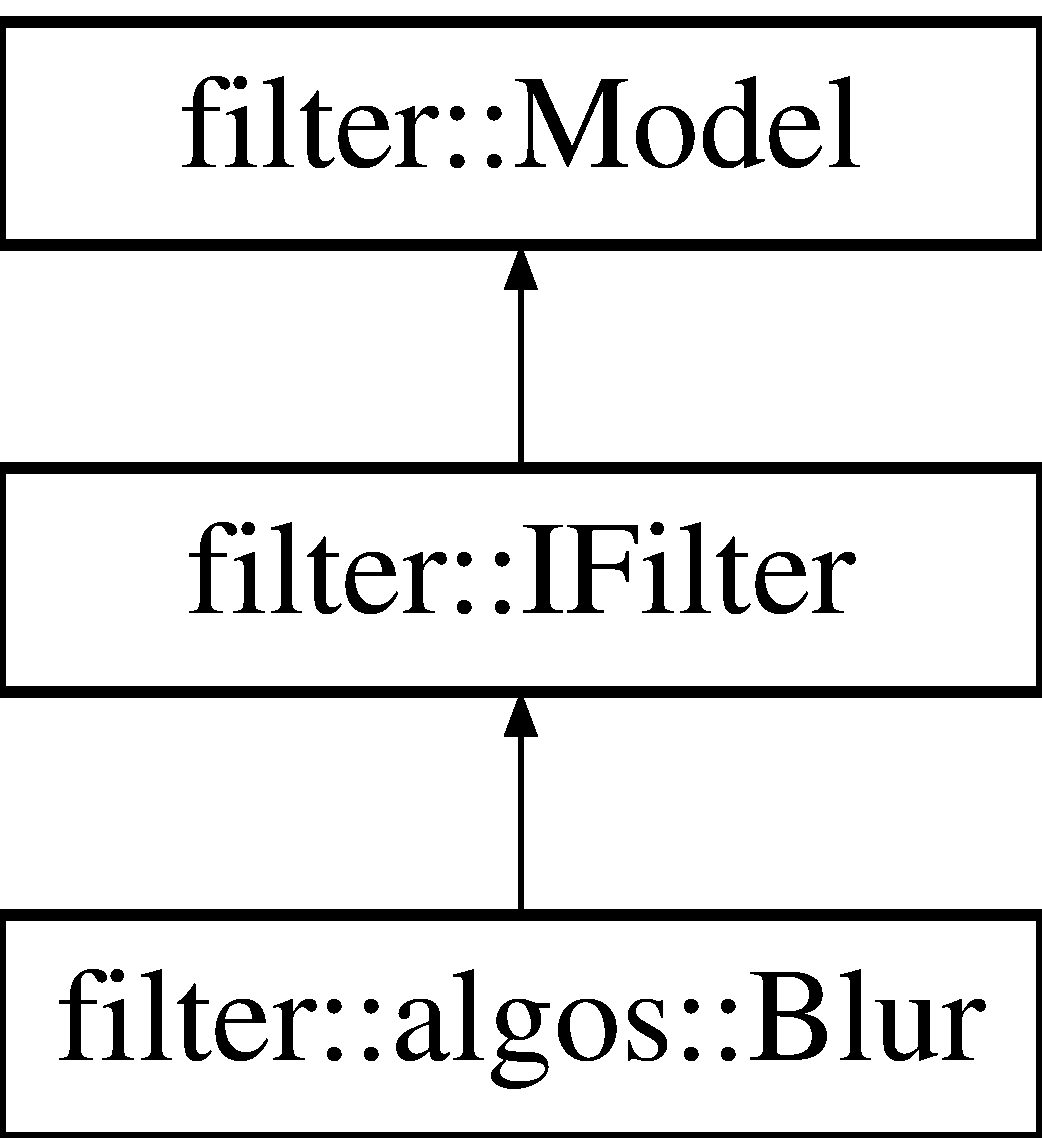
\includegraphics[height=3.000000cm]{d9/d35/classfilter_1_1algos_1_1_blur}
\end{center}
\end{figure}
\subsection*{Public Types}
\begin{DoxyCompactItemize}
\item 
\mbox{\Hypertarget{classfilter_1_1algos_1_1_blur_a573165691ed9e001beff00d0a617b76e}\label{classfilter_1_1algos_1_1_blur_a573165691ed9e001beff00d0a617b76e}} 
typedef \hyperlink{class_proxy_functor}{Proxy\+Functor}$<$ \hyperlink{classfilter_1_1algos_1_1_blur}{Blur} $>$ {\bfseries \+\_\+proxy\+Functor}
\item 
\mbox{\Hypertarget{classfilter_1_1algos_1_1_blur_a183ef1e2b7d99ac2d94e2829f2b06a6e}\label{classfilter_1_1algos_1_1_blur_a183ef1e2b7d99ac2d94e2829f2b06a6e}} 
typedef \hyperlink{classfilter_1_1algos_1_1_blur}{Blur} {\bfseries mytype}
\item 
\mbox{\Hypertarget{classfilter_1_1algos_1_1_blur_a31524be6436340debec25f4f22c8039b}\label{classfilter_1_1algos_1_1_blur_a31524be6436340debec25f4f22c8039b}} 
typedef int {\bfseries vartype\+\_\+\+\_\+kernel}
\item 
\mbox{\Hypertarget{classfilter_1_1algos_1_1_blur_a499bc97976cac8f27bf0e14a81994a5c}\label{classfilter_1_1algos_1_1_blur_a499bc97976cac8f27bf0e14a81994a5c}} 
typedef std\+::string {\bfseries vartype\+\_\+\+\_\+type}
\item 
\mbox{\Hypertarget{classfilter_1_1algos_1_1_blur_a1912f92052a7094322e72e01c177ea96}\label{classfilter_1_1algos_1_1_blur_a1912f92052a7094322e72e01c177ea96}} 
typedef double {\bfseries vartype\+\_\+\+\_\+sigmaX}
\item 
\mbox{\Hypertarget{classfilter_1_1algos_1_1_blur_a6dca814ffbe7e9702acfa2c5ec8754e5}\label{classfilter_1_1algos_1_1_blur_a6dca814ffbe7e9702acfa2c5ec8754e5}} 
typedef double {\bfseries vartype\+\_\+\+\_\+sigmaY}
\end{DoxyCompactItemize}
\subsection*{Public Member Functions}
\begin{DoxyCompactItemize}
\item 
\mbox{\Hypertarget{classfilter_1_1algos_1_1_blur_ad72f11d875fd7a6f92b6fc75214de215}\label{classfilter_1_1algos_1_1_blur_ad72f11d875fd7a6f92b6fc75214de215}} 
void {\bfseries set\+\_\+kernel\+\_\+from\+\_\+json} (boost\+::property\+\_\+tree\+::ptree \&json\+Class)
\item 
\mbox{\Hypertarget{classfilter_1_1algos_1_1_blur_a9345e902819ccef5d00c9fd48ed4b4da}\label{classfilter_1_1algos_1_1_blur_a9345e902819ccef5d00c9fd48ed4b4da}} 
void {\bfseries set\+\_\+kernel} (vartype\+\_\+\+\_\+kernel \&\+\_\+\+\_\+kernel)
\item 
\mbox{\Hypertarget{classfilter_1_1algos_1_1_blur_a678681d563c2a5db25b443d80064d51f}\label{classfilter_1_1algos_1_1_blur_a678681d563c2a5db25b443d80064d51f}} 
vartype\+\_\+\+\_\+kernel {\bfseries get\+\_\+kernel} ()
\item 
\mbox{\Hypertarget{classfilter_1_1algos_1_1_blur_ae375ae0b8e78e641b20ecd27c356fa57}\label{classfilter_1_1algos_1_1_blur_ae375ae0b8e78e641b20ecd27c356fa57}} 
void {\bfseries copy\+\_\+kernel} (\hyperlink{classfilter_1_1algos_1_1_blur}{mytype} $\ast$instance)
\item 
\mbox{\Hypertarget{classfilter_1_1algos_1_1_blur_a16091140cd5ed5c0812713d2b744d532}\label{classfilter_1_1algos_1_1_blur_a16091140cd5ed5c0812713d2b744d532}} 
void {\bfseries set\+\_\+type\+\_\+from\+\_\+json} (boost\+::property\+\_\+tree\+::ptree \&json\+Class)
\item 
\mbox{\Hypertarget{classfilter_1_1algos_1_1_blur_ab9ce4f25c743a49ca6f8659dee5c14c4}\label{classfilter_1_1algos_1_1_blur_ab9ce4f25c743a49ca6f8659dee5c14c4}} 
void {\bfseries set\+\_\+type} (vartype\+\_\+\+\_\+type \&\+\_\+\+\_\+type)
\item 
\mbox{\Hypertarget{classfilter_1_1algos_1_1_blur_a6d25c0aeaa2f58bee6385f5de4f1fc15}\label{classfilter_1_1algos_1_1_blur_a6d25c0aeaa2f58bee6385f5de4f1fc15}} 
vartype\+\_\+\+\_\+type {\bfseries get\+\_\+type} ()
\item 
\mbox{\Hypertarget{classfilter_1_1algos_1_1_blur_acdef5b8517ff686b2425e994030249f7}\label{classfilter_1_1algos_1_1_blur_acdef5b8517ff686b2425e994030249f7}} 
void {\bfseries copy\+\_\+type} (\hyperlink{classfilter_1_1algos_1_1_blur}{mytype} $\ast$instance)
\item 
\mbox{\Hypertarget{classfilter_1_1algos_1_1_blur_a11b9ae0b0735641b81a2601dcc255f34}\label{classfilter_1_1algos_1_1_blur_a11b9ae0b0735641b81a2601dcc255f34}} 
void {\bfseries set\+\_\+sigma\+X\+\_\+from\+\_\+json} (boost\+::property\+\_\+tree\+::ptree \&json\+Class)
\item 
\mbox{\Hypertarget{classfilter_1_1algos_1_1_blur_a3583c601a8b6ce4d34edb7cc54c992d1}\label{classfilter_1_1algos_1_1_blur_a3583c601a8b6ce4d34edb7cc54c992d1}} 
void {\bfseries set\+\_\+sigmaX} (vartype\+\_\+\+\_\+sigmaX \&\+\_\+\+\_\+sigmaX)
\item 
\mbox{\Hypertarget{classfilter_1_1algos_1_1_blur_a0d24fac2ff3cdbc635018f15a7e6d280}\label{classfilter_1_1algos_1_1_blur_a0d24fac2ff3cdbc635018f15a7e6d280}} 
vartype\+\_\+\+\_\+sigmaX {\bfseries get\+\_\+sigmaX} ()
\item 
\mbox{\Hypertarget{classfilter_1_1algos_1_1_blur_a587a10389382fa90b6275b11a278066a}\label{classfilter_1_1algos_1_1_blur_a587a10389382fa90b6275b11a278066a}} 
void {\bfseries copy\+\_\+sigmaX} (\hyperlink{classfilter_1_1algos_1_1_blur}{mytype} $\ast$instance)
\item 
\mbox{\Hypertarget{classfilter_1_1algos_1_1_blur_a178c7055d2d2e5a8c4a73a96df6c3030}\label{classfilter_1_1algos_1_1_blur_a178c7055d2d2e5a8c4a73a96df6c3030}} 
void {\bfseries set\+\_\+sigma\+Y\+\_\+from\+\_\+json} (boost\+::property\+\_\+tree\+::ptree \&json\+Class)
\item 
\mbox{\Hypertarget{classfilter_1_1algos_1_1_blur_a7aec769d428a23c48eb24da0c9b56d44}\label{classfilter_1_1algos_1_1_blur_a7aec769d428a23c48eb24da0c9b56d44}} 
void {\bfseries set\+\_\+sigmaY} (vartype\+\_\+\+\_\+sigmaY \&\+\_\+\+\_\+sigmaY)
\item 
\mbox{\Hypertarget{classfilter_1_1algos_1_1_blur_a6b32b9ba3d3190a0bc1ffc9d1109924b}\label{classfilter_1_1algos_1_1_blur_a6b32b9ba3d3190a0bc1ffc9d1109924b}} 
vartype\+\_\+\+\_\+sigmaY {\bfseries get\+\_\+sigmaY} ()
\item 
\mbox{\Hypertarget{classfilter_1_1algos_1_1_blur_aba890034e4207b9a930f0d425ff026a5}\label{classfilter_1_1algos_1_1_blur_aba890034e4207b9a930f0d425ff026a5}} 
void {\bfseries copy\+\_\+sigmaY} (\hyperlink{classfilter_1_1algos_1_1_blur}{mytype} $\ast$instance)
\item 
\mbox{\Hypertarget{classfilter_1_1algos_1_1_blur_a3178b579095efc92d0b0e800e12e4a29}\label{classfilter_1_1algos_1_1_blur_a3178b579095efc92d0b0e800e12e4a29}} 
Hipe\+Status {\bfseries process} () override
\end{DoxyCompactItemize}
\subsection*{Public Attributes}
\begin{DoxyCompactItemize}
\item 
int \hyperlink{classfilter_1_1algos_1_1_blur_aac3d6d8af63e5ad496fde537dc3d55aa}{kernel}
\item 
std\+::string \hyperlink{classfilter_1_1algos_1_1_blur_ac678a666d1d708d882222b198e9d9b10}{type}
\item 
double \hyperlink{classfilter_1_1algos_1_1_blur_a3b511f5fb439b9424c18141efd94b0c1}{sigmaX}
\item 
double \hyperlink{classfilter_1_1algos_1_1_blur_ac41e02492b5ab6ac6578176b11f013fc}{sigmaY}
\end{DoxyCompactItemize}
\subsection*{Private Member Functions}
\begin{DoxyCompactItemize}
\item 
\mbox{\Hypertarget{classfilter_1_1algos_1_1_blur_ae5174fbd08339457707b568a76618f2d}\label{classfilter_1_1algos_1_1_blur_ae5174fbd08339457707b568a76618f2d}} 
virtual \hyperlink{classfilter_1_1data_1_1_connex_data_base}{data\+::\+Connex\+Data\+Base} \& {\bfseries get\+Connector} ()
\end{DoxyCompactItemize}
\subsection*{Private Attributes}
\begin{DoxyCompactItemize}
\item 
\mbox{\Hypertarget{classfilter_1_1algos_1_1_blur_a5e14f95de0ecd4b9c2d7c5bb82153cc0}\label{classfilter_1_1algos_1_1_blur_a5e14f95de0ecd4b9c2d7c5bb82153cc0}} 
\hyperlink{classfilter_1_1data_1_1_connex_data}{data\+::\+Connex\+Data}$<$ \hyperlink{classfilter_1_1data_1_1_image_data}{data\+::\+Image\+Data}, \hyperlink{classfilter_1_1data_1_1_image_data}{data\+::\+Image\+Data} $>$ {\bfseries \+\_\+connex\+Data}
\end{DoxyCompactItemize}
\subsection*{Additional Inherited Members}


\subsection{Detailed Description}
The blur method can be normal (mean value of neighbouring pixels), use the median value instead of the mean, or use agaussian kernel. The user must input its desired method. \begin{DoxySeeAlso}{See also}
cv\+::blur() 

cv\+::\+Gaussian\+Blur() 

cv\+::median\+Blur() 
\end{DoxySeeAlso}


\subsection{Member Data Documentation}
\mbox{\Hypertarget{classfilter_1_1algos_1_1_blur_aac3d6d8af63e5ad496fde537dc3d55aa}\label{classfilter_1_1algos_1_1_blur_aac3d6d8af63e5ad496fde537dc3d55aa}} 
\index{filter\+::algos\+::\+Blur@{filter\+::algos\+::\+Blur}!kernel@{kernel}}
\index{kernel@{kernel}!filter\+::algos\+::\+Blur@{filter\+::algos\+::\+Blur}}
\subsubsection{\texorpdfstring{kernel}{kernel}}
{\footnotesize\ttfamily filter\+::algos\+::\+Blur\+::kernel}

The size of the kernel to use (i.\+e. the number of neighbouring pixels to evaluate). \mbox{\Hypertarget{classfilter_1_1algos_1_1_blur_a3b511f5fb439b9424c18141efd94b0c1}\label{classfilter_1_1algos_1_1_blur_a3b511f5fb439b9424c18141efd94b0c1}} 
\index{filter\+::algos\+::\+Blur@{filter\+::algos\+::\+Blur}!sigmaX@{sigmaX}}
\index{sigmaX@{sigmaX}!filter\+::algos\+::\+Blur@{filter\+::algos\+::\+Blur}}
\subsubsection{\texorpdfstring{sigmaX}{sigmaX}}
{\footnotesize\ttfamily filter\+::algos\+::\+Blur\+::sigmaX}

The gaussian kernel standard deviation in the X direction. Used only by the \hyperlink{classfilter_1_1algos_1_1_gaussian}{Gaussian} blur method. \mbox{\Hypertarget{classfilter_1_1algos_1_1_blur_ac41e02492b5ab6ac6578176b11f013fc}\label{classfilter_1_1algos_1_1_blur_ac41e02492b5ab6ac6578176b11f013fc}} 
\index{filter\+::algos\+::\+Blur@{filter\+::algos\+::\+Blur}!sigmaY@{sigmaY}}
\index{sigmaY@{sigmaY}!filter\+::algos\+::\+Blur@{filter\+::algos\+::\+Blur}}
\subsubsection{\texorpdfstring{sigmaY}{sigmaY}}
{\footnotesize\ttfamily filter\+::algos\+::\+Blur\+::sigmaY}

The gaussian kernel standard deviation in the Y direction. Used only by the \hyperlink{classfilter_1_1algos_1_1_gaussian}{Gaussian} blur method. \mbox{\Hypertarget{classfilter_1_1algos_1_1_blur_ac678a666d1d708d882222b198e9d9b10}\label{classfilter_1_1algos_1_1_blur_ac678a666d1d708d882222b198e9d9b10}} 
\index{filter\+::algos\+::\+Blur@{filter\+::algos\+::\+Blur}!type@{type}}
\index{type@{type}!filter\+::algos\+::\+Blur@{filter\+::algos\+::\+Blur}}
\subsubsection{\texorpdfstring{type}{type}}
{\footnotesize\ttfamily filter\+::algos\+::\+Blur\+::type}

The type of the blur method to use (mean, median or gaussian). 

The documentation for this class was generated from the following file\+:\begin{DoxyCompactItemize}
\item 
header/filter/\+Algos/Blur.\+h\end{DoxyCompactItemize}

\hypertarget{classfilter_1_1_algos_1_1_canny}{}\section{filter\+:\+:Algos\+:\+:Canny Class Reference}
\label{classfilter_1_1_algos_1_1_canny}\index{filter\+::\+Algos\+::\+Canny@{filter\+::\+Algos\+::\+Canny}}


The \hyperlink{classfilter_1_1_algos_1_1_canny}{Canny} filter will find the edges of the objects in an image.  




{\ttfamily \#include $<$Canny.\+h$>$}

Inheritance diagram for filter\+:\+:Algos\+:\+:Canny\+:\begin{figure}[H]
\begin{center}
\leavevmode
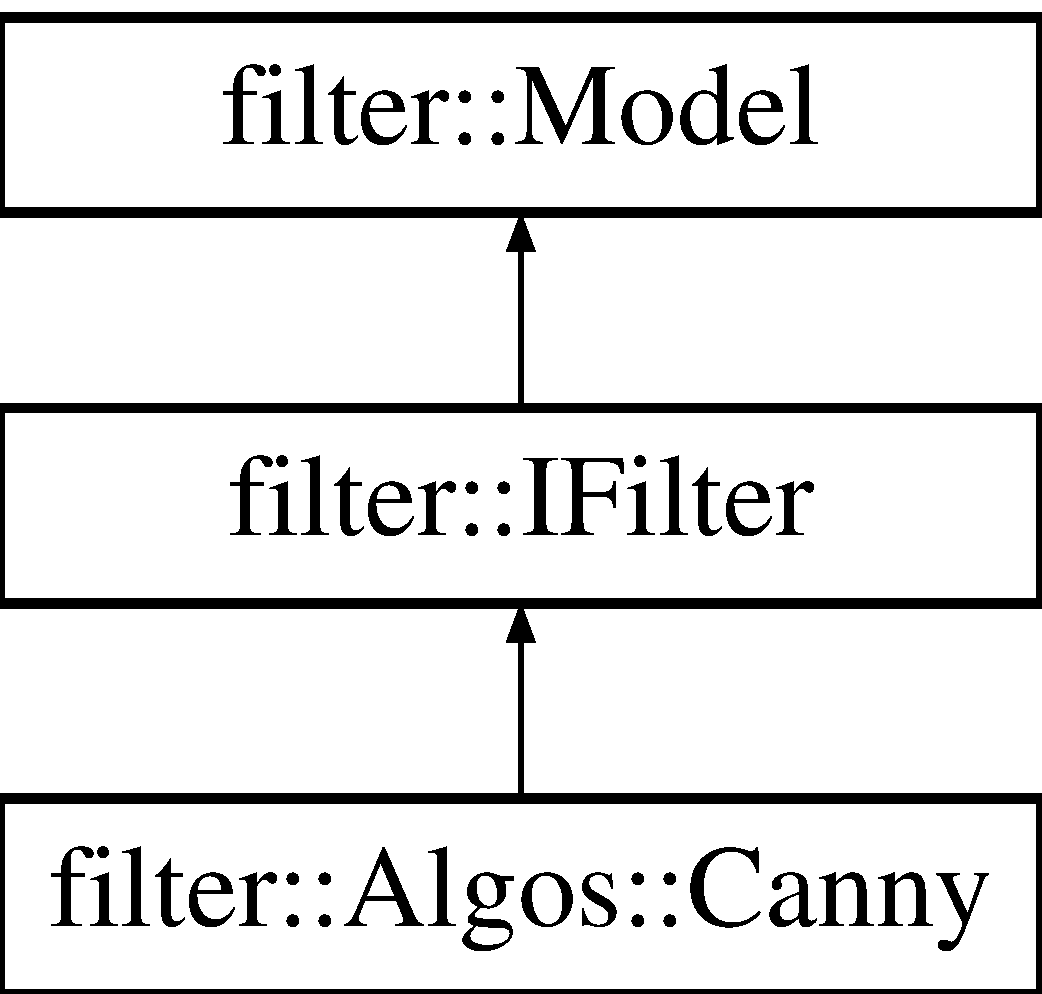
\includegraphics[height=3.000000cm]{d8/de8/classfilter_1_1_algos_1_1_canny}
\end{center}
\end{figure}
\subsection*{Public Types}
\begin{DoxyCompactItemize}
\item 
\mbox{\Hypertarget{classfilter_1_1_algos_1_1_canny_ae1d95aa394e60bb92b3f6c8fa6abf40f}\label{classfilter_1_1_algos_1_1_canny_ae1d95aa394e60bb92b3f6c8fa6abf40f}} 
typedef \hyperlink{class_proxy_functor}{Proxy\+Functor}$<$ \hyperlink{classfilter_1_1_algos_1_1_canny}{Canny} $>$ {\bfseries \+\_\+proxy\+Functor}
\item 
\mbox{\Hypertarget{classfilter_1_1_algos_1_1_canny_a39bfd0de9c93097e83e36094ef8a632c}\label{classfilter_1_1_algos_1_1_canny_a39bfd0de9c93097e83e36094ef8a632c}} 
typedef \hyperlink{classfilter_1_1_algos_1_1_canny}{Canny} {\bfseries mytype}
\item 
\mbox{\Hypertarget{classfilter_1_1_algos_1_1_canny_a2086d352adc936a92251db68c98fc57d}\label{classfilter_1_1_algos_1_1_canny_a2086d352adc936a92251db68c98fc57d}} 
typedef int {\bfseries vartype\+\_\+\+\_\+blur\+Kernel}
\item 
\mbox{\Hypertarget{classfilter_1_1_algos_1_1_canny_a0b231b846f5683be7a8cf02725d2305e}\label{classfilter_1_1_algos_1_1_canny_a0b231b846f5683be7a8cf02725d2305e}} 
typedef double {\bfseries vartype\+\_\+\+\_\+thresh1}
\item 
\mbox{\Hypertarget{classfilter_1_1_algos_1_1_canny_a368c9c004b7df6527498c7bb43928fe3}\label{classfilter_1_1_algos_1_1_canny_a368c9c004b7df6527498c7bb43928fe3}} 
typedef double {\bfseries vartype\+\_\+\+\_\+thresh2}
\item 
\mbox{\Hypertarget{classfilter_1_1_algos_1_1_canny_aa3e0af034c4b0e299f9bc61363931ee6}\label{classfilter_1_1_algos_1_1_canny_aa3e0af034c4b0e299f9bc61363931ee6}} 
typedef int {\bfseries vartype\+\_\+\+\_\+aperture}
\end{DoxyCompactItemize}
\subsection*{Public Member Functions}
\begin{DoxyCompactItemize}
\item 
\mbox{\Hypertarget{classfilter_1_1_algos_1_1_canny_a415c04c679c4fd67599332e6dfdfbd97}\label{classfilter_1_1_algos_1_1_canny_a415c04c679c4fd67599332e6dfdfbd97}} 
void {\bfseries set\+\_\+blur\+Kernel\+\_\+from\+\_\+json} (boost\+::property\+\_\+tree\+::ptree \&json\+Class)
\item 
\mbox{\Hypertarget{classfilter_1_1_algos_1_1_canny_a980c9ffdd9ccfb2a1163cff05690ab75}\label{classfilter_1_1_algos_1_1_canny_a980c9ffdd9ccfb2a1163cff05690ab75}} 
void {\bfseries set\+\_\+blur\+Kernel} (vartype\+\_\+\+\_\+blur\+Kernel \&\+\_\+\+\_\+blur\+Kernel)
\item 
\mbox{\Hypertarget{classfilter_1_1_algos_1_1_canny_a28f904d59c5e5327a7d69bcbc9d1b5d6}\label{classfilter_1_1_algos_1_1_canny_a28f904d59c5e5327a7d69bcbc9d1b5d6}} 
vartype\+\_\+\+\_\+blur\+Kernel {\bfseries get\+\_\+blur\+Kernel} ()
\item 
\mbox{\Hypertarget{classfilter_1_1_algos_1_1_canny_a75294ab8de76fd7751713d12db806d26}\label{classfilter_1_1_algos_1_1_canny_a75294ab8de76fd7751713d12db806d26}} 
void {\bfseries copy\+\_\+blur\+Kernel} (\hyperlink{classfilter_1_1_algos_1_1_canny}{mytype} $\ast$instance)
\item 
\mbox{\Hypertarget{classfilter_1_1_algos_1_1_canny_a8f9b7b30c6a02a8851914be4af6e8687}\label{classfilter_1_1_algos_1_1_canny_a8f9b7b30c6a02a8851914be4af6e8687}} 
void {\bfseries set\+\_\+thresh1\+\_\+from\+\_\+json} (boost\+::property\+\_\+tree\+::ptree \&json\+Class)
\item 
\mbox{\Hypertarget{classfilter_1_1_algos_1_1_canny_a85e52973f0d094a9371f865132a2052d}\label{classfilter_1_1_algos_1_1_canny_a85e52973f0d094a9371f865132a2052d}} 
void {\bfseries set\+\_\+thresh1} (vartype\+\_\+\+\_\+thresh1 \&\+\_\+\+\_\+thresh1)
\item 
\mbox{\Hypertarget{classfilter_1_1_algos_1_1_canny_a83c3b6077acb089393323637e14ec557}\label{classfilter_1_1_algos_1_1_canny_a83c3b6077acb089393323637e14ec557}} 
vartype\+\_\+\+\_\+thresh1 {\bfseries get\+\_\+thresh1} ()
\item 
\mbox{\Hypertarget{classfilter_1_1_algos_1_1_canny_ab13aa4863bd252c5be652ad0c6e32848}\label{classfilter_1_1_algos_1_1_canny_ab13aa4863bd252c5be652ad0c6e32848}} 
void {\bfseries copy\+\_\+thresh1} (\hyperlink{classfilter_1_1_algos_1_1_canny}{mytype} $\ast$instance)
\item 
\mbox{\Hypertarget{classfilter_1_1_algos_1_1_canny_a0e04b7d9c830c46d8598365eab5838c9}\label{classfilter_1_1_algos_1_1_canny_a0e04b7d9c830c46d8598365eab5838c9}} 
void {\bfseries set\+\_\+thresh2\+\_\+from\+\_\+json} (boost\+::property\+\_\+tree\+::ptree \&json\+Class)
\item 
\mbox{\Hypertarget{classfilter_1_1_algos_1_1_canny_a9ba95744ecff03d4ff3058ca8bfb9b71}\label{classfilter_1_1_algos_1_1_canny_a9ba95744ecff03d4ff3058ca8bfb9b71}} 
void {\bfseries set\+\_\+thresh2} (vartype\+\_\+\+\_\+thresh2 \&\+\_\+\+\_\+thresh2)
\item 
\mbox{\Hypertarget{classfilter_1_1_algos_1_1_canny_a89788968370de3013a1217f01484c657}\label{classfilter_1_1_algos_1_1_canny_a89788968370de3013a1217f01484c657}} 
vartype\+\_\+\+\_\+thresh2 {\bfseries get\+\_\+thresh2} ()
\item 
\mbox{\Hypertarget{classfilter_1_1_algos_1_1_canny_ab130fd69c99eaff0cba194f122d63eb9}\label{classfilter_1_1_algos_1_1_canny_ab130fd69c99eaff0cba194f122d63eb9}} 
void {\bfseries copy\+\_\+thresh2} (\hyperlink{classfilter_1_1_algos_1_1_canny}{mytype} $\ast$instance)
\item 
\mbox{\Hypertarget{classfilter_1_1_algos_1_1_canny_ab8f1c063ff8bfa04c8cbc271c6aa6ac0}\label{classfilter_1_1_algos_1_1_canny_ab8f1c063ff8bfa04c8cbc271c6aa6ac0}} 
void {\bfseries set\+\_\+aperture\+\_\+from\+\_\+json} (boost\+::property\+\_\+tree\+::ptree \&json\+Class)
\item 
\mbox{\Hypertarget{classfilter_1_1_algos_1_1_canny_a86cc6ffcc91f0a57d6c85fafda3e51b7}\label{classfilter_1_1_algos_1_1_canny_a86cc6ffcc91f0a57d6c85fafda3e51b7}} 
void {\bfseries set\+\_\+aperture} (vartype\+\_\+\+\_\+aperture \&\+\_\+\+\_\+aperture)
\item 
\mbox{\Hypertarget{classfilter_1_1_algos_1_1_canny_acaf64fb37abb79cfdea926c299e5ac50}\label{classfilter_1_1_algos_1_1_canny_acaf64fb37abb79cfdea926c299e5ac50}} 
vartype\+\_\+\+\_\+aperture {\bfseries get\+\_\+aperture} ()
\item 
\mbox{\Hypertarget{classfilter_1_1_algos_1_1_canny_a97ebfc5c2393ccffce843fa7c827b606}\label{classfilter_1_1_algos_1_1_canny_a97ebfc5c2393ccffce843fa7c827b606}} 
void {\bfseries copy\+\_\+aperture} (\hyperlink{classfilter_1_1_algos_1_1_canny}{mytype} $\ast$instance)
\item 
\mbox{\Hypertarget{classfilter_1_1_algos_1_1_canny_a78f9f89095319c36ba8d5ea341a017c0}\label{classfilter_1_1_algos_1_1_canny_a78f9f89095319c36ba8d5ea341a017c0}} 
Hipe\+Status {\bfseries process} () override
\end{DoxyCompactItemize}
\subsection*{Public Attributes}
\begin{DoxyCompactItemize}
\item 
int \hyperlink{classfilter_1_1_algos_1_1_canny_ab76f95b183fd0e59518b6f65b9345ad0}{blur\+Kernel}
\item 
double \hyperlink{classfilter_1_1_algos_1_1_canny_a7ca25f641a06d01a0467122fb22ad947}{thresh1}
\item 
double \hyperlink{classfilter_1_1_algos_1_1_canny_abccf54314a60ab802a99b47983436938}{thresh2}
\item 
int \hyperlink{classfilter_1_1_algos_1_1_canny_a73d61bdf0d7c6cd77af2b3d5b609cfc5}{aperture}
\end{DoxyCompactItemize}
\subsection*{Private Member Functions}
\begin{DoxyCompactItemize}
\item 
\mbox{\Hypertarget{classfilter_1_1_algos_1_1_canny_a1c45ed066b15b77e2e44d5565d519591}\label{classfilter_1_1_algos_1_1_canny_a1c45ed066b15b77e2e44d5565d519591}} 
virtual \hyperlink{classfilter_1_1data_1_1_connex_data_base}{data\+::\+Connex\+Data\+Base} \& {\bfseries get\+Connector} ()
\end{DoxyCompactItemize}
\subsection*{Private Attributes}
\begin{DoxyCompactItemize}
\item 
\mbox{\Hypertarget{classfilter_1_1_algos_1_1_canny_ae592fc78df0f5417418ec02b1a5dd763}\label{classfilter_1_1_algos_1_1_canny_ae592fc78df0f5417418ec02b1a5dd763}} 
\hyperlink{classfilter_1_1data_1_1_connex_data}{data\+::\+Connex\+Data}$<$ \hyperlink{classfilter_1_1data_1_1_image_data}{data\+::\+Image\+Data}, \hyperlink{classfilter_1_1data_1_1_image_data}{data\+::\+Image\+Data} $>$ {\bfseries \+\_\+connex\+Data}
\end{DoxyCompactItemize}
\subsection*{Additional Inherited Members}


\subsection{Detailed Description}
The image needs to be in grayscale. If not it will be converted at runtime. The filter will first blur the image (for better results), then use the canny algorithm. The output of the canny algorithm will help to find the contours with the Open\+CV find\+Contours function. \begin{DoxySeeAlso}{See also}
cv\+::\+Canny() 

cv\+::find\+Contours() 
\end{DoxySeeAlso}


\subsection{Member Data Documentation}
\mbox{\Hypertarget{classfilter_1_1_algos_1_1_canny_a73d61bdf0d7c6cd77af2b3d5b609cfc5}\label{classfilter_1_1_algos_1_1_canny_a73d61bdf0d7c6cd77af2b3d5b609cfc5}} 
\index{filter\+::\+Algos\+::\+Canny@{filter\+::\+Algos\+::\+Canny}!aperture@{aperture}}
\index{aperture@{aperture}!filter\+::\+Algos\+::\+Canny@{filter\+::\+Algos\+::\+Canny}}
\subsubsection{\texorpdfstring{aperture}{aperture}}
{\footnotesize\ttfamily filter\+::\+Algos\+::\+Canny\+::aperture}

The aperture size for the sobel operator. \begin{DoxySeeAlso}{See also}
cv\+::\+Sobel() 
\end{DoxySeeAlso}
\mbox{\Hypertarget{classfilter_1_1_algos_1_1_canny_ab76f95b183fd0e59518b6f65b9345ad0}\label{classfilter_1_1_algos_1_1_canny_ab76f95b183fd0e59518b6f65b9345ad0}} 
\index{filter\+::\+Algos\+::\+Canny@{filter\+::\+Algos\+::\+Canny}!blur\+Kernel@{blur\+Kernel}}
\index{blur\+Kernel@{blur\+Kernel}!filter\+::\+Algos\+::\+Canny@{filter\+::\+Algos\+::\+Canny}}
\subsubsection{\texorpdfstring{blur\+Kernel}{blurKernel}}
{\footnotesize\ttfamily filter\+::\+Algos\+::\+Canny\+::blur\+Kernel}

The size of the blur kernel to use. \begin{DoxySeeAlso}{See also}
cv\+::blur() 
\end{DoxySeeAlso}
\mbox{\Hypertarget{classfilter_1_1_algos_1_1_canny_a7ca25f641a06d01a0467122fb22ad947}\label{classfilter_1_1_algos_1_1_canny_a7ca25f641a06d01a0467122fb22ad947}} 
\index{filter\+::\+Algos\+::\+Canny@{filter\+::\+Algos\+::\+Canny}!thresh1@{thresh1}}
\index{thresh1@{thresh1}!filter\+::\+Algos\+::\+Canny@{filter\+::\+Algos\+::\+Canny}}
\subsubsection{\texorpdfstring{thresh1}{thresh1}}
{\footnotesize\ttfamily filter\+::\+Algos\+::\+Canny\+::thresh1}

The first threshold for the canny\textquotesingle{}s hysteresis procedure. \mbox{\Hypertarget{classfilter_1_1_algos_1_1_canny_abccf54314a60ab802a99b47983436938}\label{classfilter_1_1_algos_1_1_canny_abccf54314a60ab802a99b47983436938}} 
\index{filter\+::\+Algos\+::\+Canny@{filter\+::\+Algos\+::\+Canny}!thresh2@{thresh2}}
\index{thresh2@{thresh2}!filter\+::\+Algos\+::\+Canny@{filter\+::\+Algos\+::\+Canny}}
\subsubsection{\texorpdfstring{thresh2}{thresh2}}
{\footnotesize\ttfamily filter\+::\+Algos\+::\+Canny\+::thresh2}

The second threshold for the canny\textquotesingle{}s hysteresis procedure. 

The documentation for this class was generated from the following file\+:\begin{DoxyCompactItemize}
\item 
header/filter/\+Algos/Canny.\+h\end{DoxyCompactItemize}

\hypertarget{class_capture_video}{}\section{Capture\+Video Class Reference}
\label{class_capture_video}\index{Capture\+Video@{Capture\+Video}}
Inheritance diagram for Capture\+Video\+:\begin{figure}[H]
\begin{center}
\leavevmode
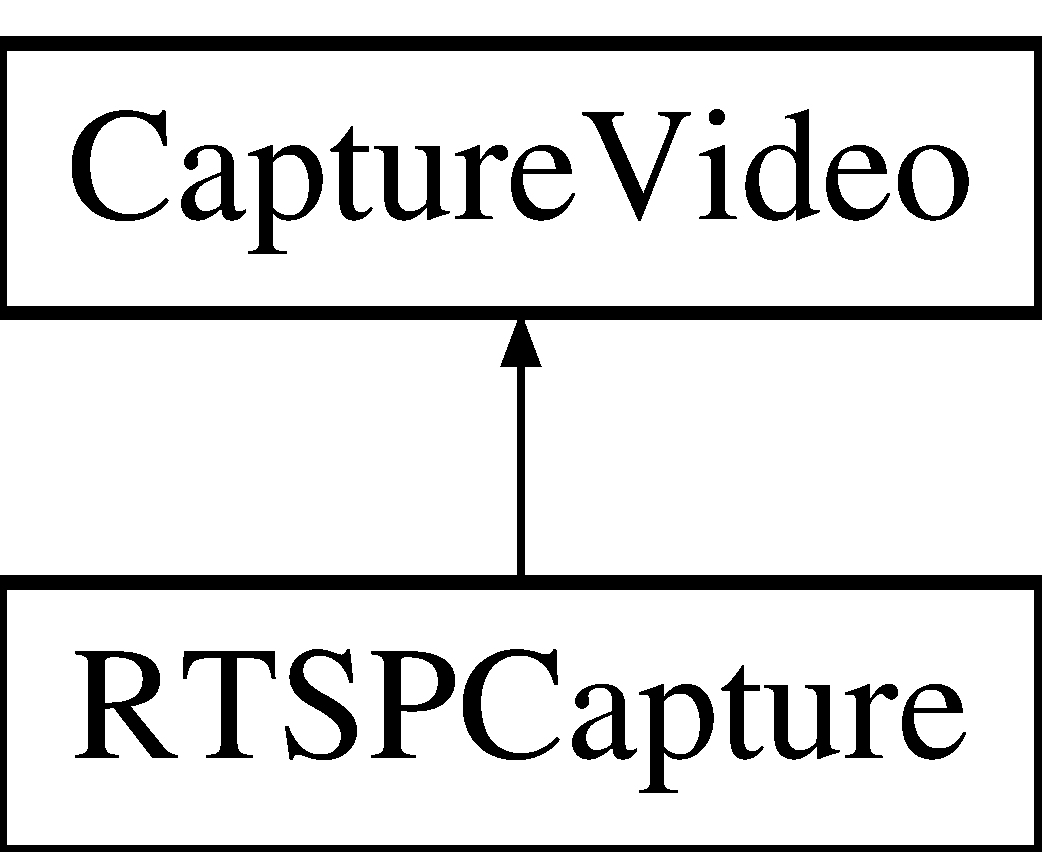
\includegraphics[height=2.000000cm]{d4/d6c/class_capture_video}
\end{center}
\end{figure}
\subsection*{Public Member Functions}
\begin{DoxyCompactItemize}
\item 
\mbox{\Hypertarget{class_capture_video_aaac435b2fdcec0cb8ca674e7f1a6954d}\label{class_capture_video_aaac435b2fdcec0cb8ca674e7f1a6954d}} 
{\bfseries Capture\+Video} (const std\+::string \&path)
\item 
\mbox{\Hypertarget{class_capture_video_ac8d911e838ab70d49b219ff3490e0deb}\label{class_capture_video_ac8d911e838ab70d49b219ff3490e0deb}} 
virtual Hipe\+Status {\bfseries open} ()
\item 
\mbox{\Hypertarget{class_capture_video_ac0a442aa7e3b947a1975e9801e4b7ca3}\label{class_capture_video_ac0a442aa7e3b947a1975e9801e4b7ca3}} 
virtual Hipe\+Status {\bfseries close} ()
\item 
\mbox{\Hypertarget{class_capture_video_a6dfcb36a508c7af1d9fedcc9df5b9c9b}\label{class_capture_video_a6dfcb36a508c7af1d9fedcc9df5b9c9b}} 
virtual Hipe\+Status {\bfseries destroy} ()
\item 
\mbox{\Hypertarget{class_capture_video_afc5fbb5d946d34a815dbbf2c1ab71ff6}\label{class_capture_video_afc5fbb5d946d34a815dbbf2c1ab71ff6}} 
virtual Hipe\+Status {\bfseries create} ()
\item 
\mbox{\Hypertarget{class_capture_video_a2c3fca6a34c82b151cc915747399dff9}\label{class_capture_video_a2c3fca6a34c82b151cc915747399dff9}} 
virtual Hipe\+Status {\bfseries read} (cv\+::\+Mat \&image)
\end{DoxyCompactItemize}
\subsection*{Protected Attributes}
\begin{DoxyCompactItemize}
\item 
\mbox{\Hypertarget{class_capture_video_aa4af6fcb50ba52f08a545b7355719775}\label{class_capture_video_aa4af6fcb50ba52f08a545b7355719775}} 
const std\+::string {\bfseries \+\_\+path}
\end{DoxyCompactItemize}


The documentation for this class was generated from the following file\+:\begin{DoxyCompactItemize}
\item 
header/streaming/Capture\+Video.\+h\end{DoxyCompactItemize}

\hypertarget{class_capture_video_factory}{}\section{Capture\+Video\+Factory Class Reference}
\label{class_capture_video_factory}\index{Capture\+Video\+Factory@{Capture\+Video\+Factory}}
Inheritance diagram for Capture\+Video\+Factory\+:\begin{figure}[H]
\begin{center}
\leavevmode
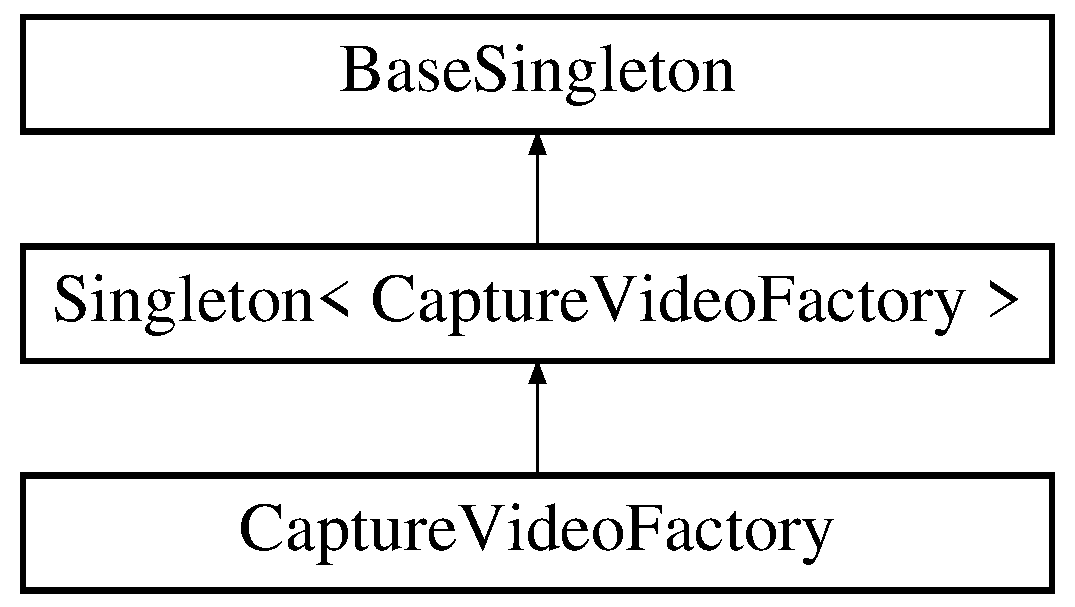
\includegraphics[height=3.000000cm]{d6/d4b/class_capture_video_factory}
\end{center}
\end{figure}
\subsection*{Public Member Functions}
\begin{DoxyCompactItemize}
\item 
\mbox{\Hypertarget{class_capture_video_factory_aa697f4a0893d7d5e023d0b69982bd7f1}\label{class_capture_video_factory_aa697f4a0893d7d5e023d0b69982bd7f1}} 
\hyperlink{class_capture_video}{Capture\+Video} $\ast$ {\bfseries get\+Capture\+Video} (std\+::string \&capture\+Video\+Name, const std\+::string \&path)
\end{DoxyCompactItemize}
\subsection*{Protected Attributes}
\begin{DoxyCompactItemize}
\item 
\mbox{\Hypertarget{class_capture_video_factory_a748d0309d4f63f0c4d9cf5c642458637}\label{class_capture_video_factory_a748d0309d4f63f0c4d9cf5c642458637}} 
std\+::map$<$ std\+::string, \hyperlink{class_capture_video}{Capture\+Video} $\ast$ $>$ {\bfseries \+\_\+capture\+Video\+Table}
\item 
\mbox{\Hypertarget{class_capture_video_factory_afdbe26984eff4b7fc17a016403416723}\label{class_capture_video_factory_afdbe26984eff4b7fc17a016403416723}} 
std\+::mutex {\bfseries locking}
\end{DoxyCompactItemize}
\subsection*{Additional Inherited Members}


The documentation for this class was generated from the following files\+:\begin{DoxyCompactItemize}
\item 
header/streaming/Capture\+Video.\+h\item 
source/streaming/Capture\+Video.\+cpp\end{DoxyCompactItemize}

\hypertarget{classhttp_1_1_client}{}\section{http\+:\+:Client$<$ socket\+\_\+type $>$ Class Template Reference}
\label{classhttp_1_1_client}\index{http\+::\+Client$<$ socket\+\_\+type $>$@{http\+::\+Client$<$ socket\+\_\+type $>$}}
Inheritance diagram for http\+:\+:Client$<$ socket\+\_\+type $>$\+:\begin{figure}[H]
\begin{center}
\leavevmode
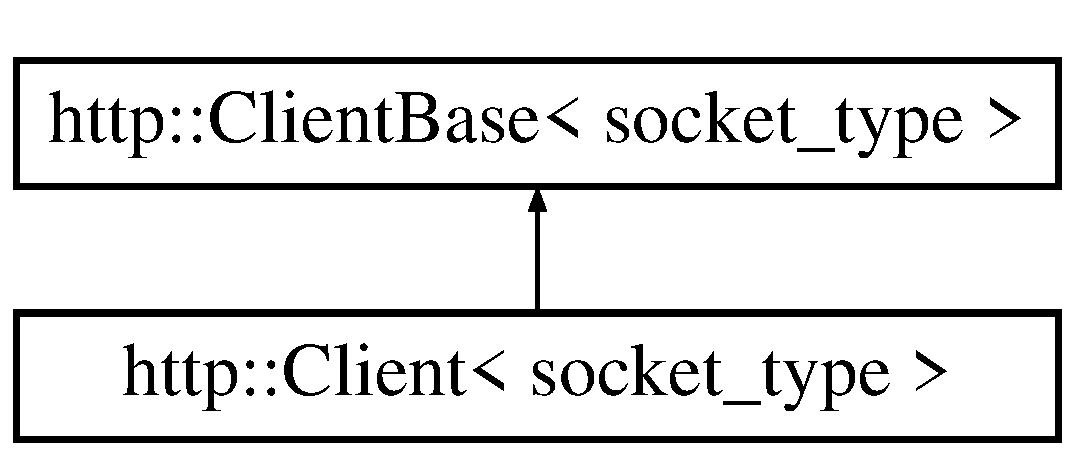
\includegraphics[height=2.000000cm]{d2/d35/classhttp_1_1_client}
\end{center}
\end{figure}
\subsection*{Additional Inherited Members}


The documentation for this class was generated from the following file\+:\begin{DoxyCompactItemize}
\item 
header/http/Http\+Client.\+h\end{DoxyCompactItemize}

\hypertarget{classhttp_1_1_client_3_01_h_t_t_p_01_4}{}\section{http\+:\+:Client$<$ H\+T\+TP $>$ Class Template Reference}
\label{classhttp_1_1_client_3_01_h_t_t_p_01_4}\index{http\+::\+Client$<$ H\+T\+T\+P $>$@{http\+::\+Client$<$ H\+T\+T\+P $>$}}
Inheritance diagram for http\+:\+:Client$<$ H\+T\+TP $>$\+:\begin{figure}[H]
\begin{center}
\leavevmode
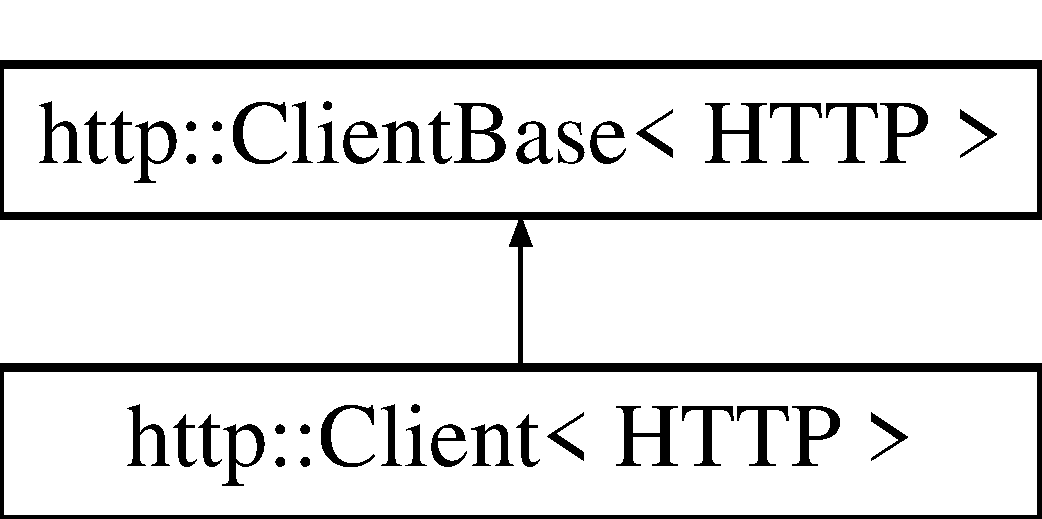
\includegraphics[height=2.000000cm]{d4/da7/classhttp_1_1_client_3_01_h_t_t_p_01_4}
\end{center}
\end{figure}
\subsection*{Public Member Functions}
\begin{DoxyCompactItemize}
\item 
\mbox{\Hypertarget{classhttp_1_1_client_3_01_h_t_t_p_01_4_a1ff860c7e44f554b04022fed43dcdf94}\label{classhttp_1_1_client_3_01_h_t_t_p_01_4_a1ff860c7e44f554b04022fed43dcdf94}} 
{\bfseries Client} (const std\+::string \&server\+\_\+port\+\_\+path)
\end{DoxyCompactItemize}
\subsection*{Protected Member Functions}
\begin{DoxyCompactItemize}
\item 
\mbox{\Hypertarget{classhttp_1_1_client_3_01_h_t_t_p_01_4_a356b4f8f63662c9e5bb22895ed2fe7f3}\label{classhttp_1_1_client_3_01_h_t_t_p_01_4_a356b4f8f63662c9e5bb22895ed2fe7f3}} 
void {\bfseries connect} ()
\end{DoxyCompactItemize}
\subsection*{Additional Inherited Members}


The documentation for this class was generated from the following file\+:\begin{DoxyCompactItemize}
\item 
header/http/Http\+Client.\+h\end{DoxyCompactItemize}

\hypertarget{classhttp_1_1_client_base}{}\section{http\+:\+:Client\+Base$<$ socket\+\_\+type $>$ Class Template Reference}
\label{classhttp_1_1_client_base}\index{http\+::\+Client\+Base$<$ socket\+\_\+type $>$@{http\+::\+Client\+Base$<$ socket\+\_\+type $>$}}
Inheritance diagram for http\+:\+:Client\+Base$<$ socket\+\_\+type $>$\+:\begin{figure}[H]
\begin{center}
\leavevmode
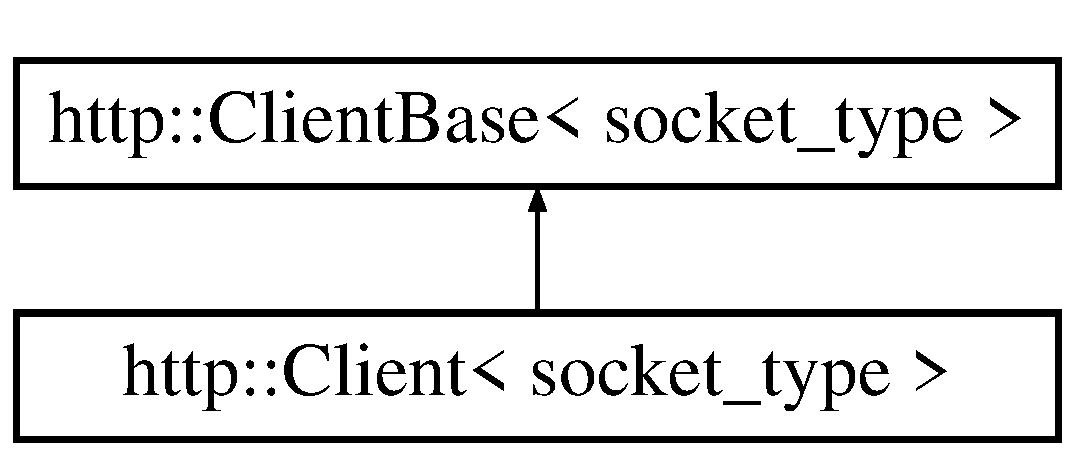
\includegraphics[height=2.000000cm]{d2/d7e/classhttp_1_1_client_base}
\end{center}
\end{figure}
\subsection*{Classes}
\begin{DoxyCompactItemize}
\item 
class \hyperlink{classhttp_1_1_client_base_1_1_config}{Config}
\item 
class \hyperlink{classhttp_1_1_client_base_1_1_response}{Response}
\end{DoxyCompactItemize}
\subsection*{Public Member Functions}
\begin{DoxyCompactItemize}
\item 
\mbox{\Hypertarget{classhttp_1_1_client_base_a3e625144c683838d9731b071d25570c2}\label{classhttp_1_1_client_base_a3e625144c683838d9731b071d25570c2}} 
std\+::shared\+\_\+ptr$<$ \hyperlink{classhttp_1_1_client_base_1_1_response}{Response} $>$ {\bfseries request} (const std\+::string \&request\+\_\+type, const std\+::string \&path=\char`\"{}/\char`\"{}, boost\+::string\+\_\+ref content=\char`\"{}\char`\"{}, const std\+::map$<$ std\+::string, std\+::string $>$ \&header=std\+::map$<$ std\+::string, std\+::string $>$())
\item 
\mbox{\Hypertarget{classhttp_1_1_client_base_a73afa2fcfa3f9991dcf3590e503de569}\label{classhttp_1_1_client_base_a73afa2fcfa3f9991dcf3590e503de569}} 
std\+::shared\+\_\+ptr$<$ \hyperlink{classhttp_1_1_client_base_1_1_response}{Response} $>$ {\bfseries request} (const std\+::string \&request\+\_\+type, const std\+::string \&path, std\+::iostream \&content, const std\+::map$<$ std\+::string, std\+::string $>$ \&header=std\+::map$<$ std\+::string, std\+::string $>$())
\item 
\mbox{\Hypertarget{classhttp_1_1_client_base_a98810f3e43a414012a07862384cb095f}\label{classhttp_1_1_client_base_a98810f3e43a414012a07862384cb095f}} 
void {\bfseries close} ()
\end{DoxyCompactItemize}
\subsection*{Public Attributes}
\begin{DoxyCompactItemize}
\item 
\mbox{\Hypertarget{classhttp_1_1_client_base_a3810388b54d19e5f020d3eca8d08d470}\label{classhttp_1_1_client_base_a3810388b54d19e5f020d3eca8d08d470}} 
\hyperlink{classhttp_1_1_client_base_1_1_config}{Config} \hyperlink{classhttp_1_1_client_base_a3810388b54d19e5f020d3eca8d08d470}{config}
\begin{DoxyCompactList}\small\item\em Set before calling request. \end{DoxyCompactList}\end{DoxyCompactItemize}
\subsection*{Protected Member Functions}
\begin{DoxyCompactItemize}
\item 
\mbox{\Hypertarget{classhttp_1_1_client_base_a2ff65d90b13a6023365c24c262d225db}\label{classhttp_1_1_client_base_a2ff65d90b13a6023365c24c262d225db}} 
{\bfseries Client\+Base} (const std\+::string \&host\+\_\+port, unsigned short default\+\_\+port)
\item 
\mbox{\Hypertarget{classhttp_1_1_client_base_ad7961a2aa770956abdba876ca71c7e44}\label{classhttp_1_1_client_base_ad7961a2aa770956abdba876ca71c7e44}} 
std\+::pair$<$ std\+::string, unsigned short $>$ {\bfseries parse\+\_\+host\+\_\+port} (const std\+::string \&host\+\_\+port, unsigned short default\+\_\+port)
\item 
\mbox{\Hypertarget{classhttp_1_1_client_base_adeded9b02b837389f6cc9805237255d8}\label{classhttp_1_1_client_base_adeded9b02b837389f6cc9805237255d8}} 
virtual void {\bfseries connect} ()=0
\item 
\mbox{\Hypertarget{classhttp_1_1_client_base_a35344900c1a5a847b5cad6e71683388e}\label{classhttp_1_1_client_base_a35344900c1a5a847b5cad6e71683388e}} 
std\+::shared\+\_\+ptr$<$ boost\+::asio\+::deadline\+\_\+timer $>$ {\bfseries get\+\_\+timeout\+\_\+timer} ()
\item 
\mbox{\Hypertarget{classhttp_1_1_client_base_a9a974d37fdd95968ee952f8bd923c4cf}\label{classhttp_1_1_client_base_a9a974d37fdd95968ee952f8bd923c4cf}} 
void {\bfseries parse\+\_\+response\+\_\+header} (const std\+::shared\+\_\+ptr$<$ \hyperlink{classhttp_1_1_client_base_1_1_response}{Response} $>$ \&response) const
\item 
\mbox{\Hypertarget{classhttp_1_1_client_base_ac755547ec13040504a2d26af90c6042f}\label{classhttp_1_1_client_base_ac755547ec13040504a2d26af90c6042f}} 
std\+::shared\+\_\+ptr$<$ \hyperlink{classhttp_1_1_client_base_1_1_response}{Response} $>$ {\bfseries request\+\_\+read} ()
\item 
\mbox{\Hypertarget{classhttp_1_1_client_base_a83b002bc7cd15da4d817d48e077d74ab}\label{classhttp_1_1_client_base_a83b002bc7cd15da4d817d48e077d74ab}} 
void {\bfseries request\+\_\+read\+\_\+chunked} (const std\+::shared\+\_\+ptr$<$ \hyperlink{classhttp_1_1_client_base_1_1_response}{Response} $>$ \&response, boost\+::asio\+::streambuf \&streambuf)
\end{DoxyCompactItemize}
\subsection*{Protected Attributes}
\begin{DoxyCompactItemize}
\item 
\mbox{\Hypertarget{classhttp_1_1_client_base_ae05a4e6734fc913d0c8072950c580371}\label{classhttp_1_1_client_base_ae05a4e6734fc913d0c8072950c580371}} 
boost\+::asio\+::io\+\_\+service {\bfseries io\+\_\+service}
\item 
\mbox{\Hypertarget{classhttp_1_1_client_base_aeafcca58376a64522dd0b17300097926}\label{classhttp_1_1_client_base_aeafcca58376a64522dd0b17300097926}} 
boost\+::asio\+::ip\+::tcp\+::resolver {\bfseries resolver}
\item 
\mbox{\Hypertarget{classhttp_1_1_client_base_ae9194e0064360446237a43056df0d881}\label{classhttp_1_1_client_base_ae9194e0064360446237a43056df0d881}} 
std\+::unique\+\_\+ptr$<$ socket\+\_\+type $>$ {\bfseries socket}
\item 
\mbox{\Hypertarget{classhttp_1_1_client_base_a57456c0e9ef28f44f7ba69c0539e80da}\label{classhttp_1_1_client_base_a57456c0e9ef28f44f7ba69c0539e80da}} 
std\+::mutex {\bfseries socket\+\_\+mutex}
\item 
\mbox{\Hypertarget{classhttp_1_1_client_base_abfc8afff192657d6526e209d85c64698}\label{classhttp_1_1_client_base_abfc8afff192657d6526e209d85c64698}} 
std\+::string {\bfseries host}
\item 
\mbox{\Hypertarget{classhttp_1_1_client_base_af99a277d82044059d66db06dbb38cf16}\label{classhttp_1_1_client_base_af99a277d82044059d66db06dbb38cf16}} 
unsigned short {\bfseries port}
\end{DoxyCompactItemize}


The documentation for this class was generated from the following file\+:\begin{DoxyCompactItemize}
\item 
header/http/Http\+Client.\+h\end{DoxyCompactItemize}

\hypertarget{classfilter_1_1algos_1_1_closest_color}{}\section{filter\+:\+:algos\+:\+:Closest\+Color Class Reference}
\label{classfilter_1_1algos_1_1_closest_color}\index{filter\+::algos\+::\+Closest\+Color@{filter\+::algos\+::\+Closest\+Color}}


The \hyperlink{classfilter_1_1algos_1_1_closest_color}{Closest\+Color} filter will find the closest known color a pixel have. The input image must only contain 1 pixel.  




{\ttfamily \#include $<$Closest\+Color.\+h$>$}

Inheritance diagram for filter\+:\+:algos\+:\+:Closest\+Color\+:\begin{figure}[H]
\begin{center}
\leavevmode
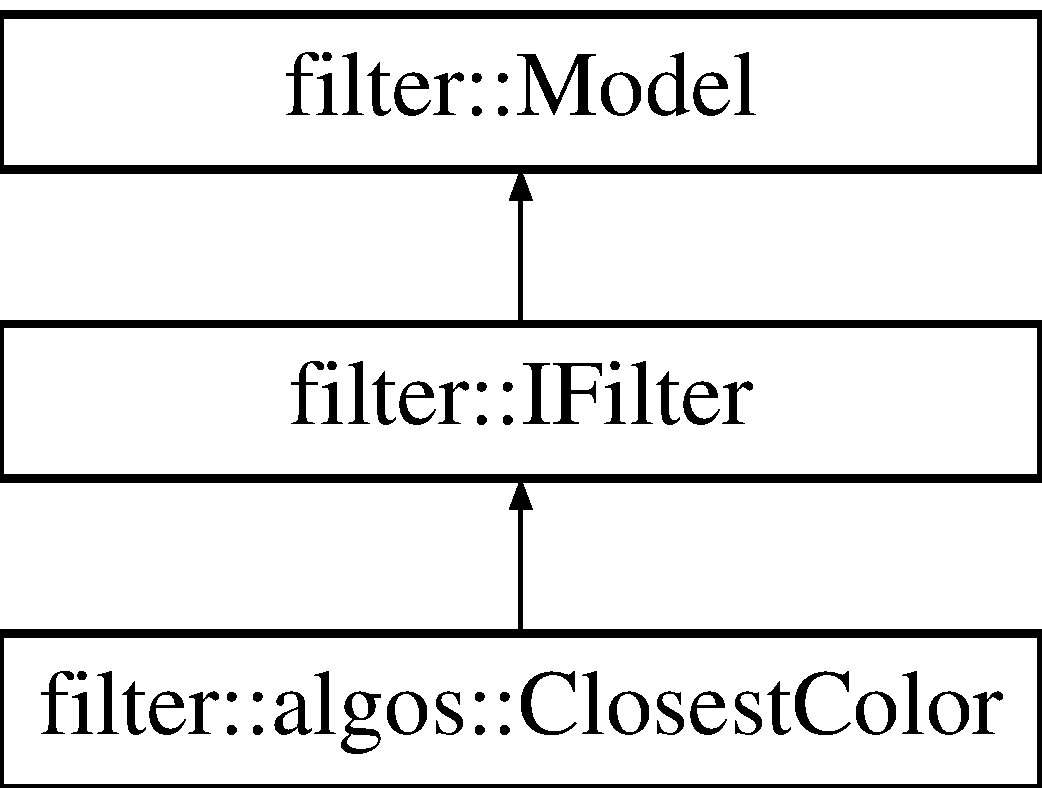
\includegraphics[height=3.000000cm]{d1/d1c/classfilter_1_1algos_1_1_closest_color}
\end{center}
\end{figure}
\subsection*{Classes}
\begin{DoxyCompactItemize}
\item 
struct \hyperlink{structfilter_1_1algos_1_1_closest_color_1_1_color}{Color}
\begin{DoxyCompactList}\small\item\em The representation of a color. \end{DoxyCompactList}\end{DoxyCompactItemize}
\subsection*{Public Types}
\begin{DoxyCompactItemize}
\item 
\mbox{\Hypertarget{classfilter_1_1algos_1_1_closest_color_ae0a71e75e3c30026ca08d255c3ef435d}\label{classfilter_1_1algos_1_1_closest_color_ae0a71e75e3c30026ca08d255c3ef435d}} 
typedef \hyperlink{class_proxy_functor}{Proxy\+Functor}$<$ \hyperlink{classfilter_1_1algos_1_1_closest_color}{Closest\+Color} $>$ {\bfseries \+\_\+proxy\+Functor}
\item 
\mbox{\Hypertarget{classfilter_1_1algos_1_1_closest_color_a20d50a313d53f976513d839c5be7e141}\label{classfilter_1_1algos_1_1_closest_color_a20d50a313d53f976513d839c5be7e141}} 
typedef \hyperlink{classfilter_1_1algos_1_1_closest_color}{Closest\+Color} {\bfseries mytype}
\item 
\mbox{\Hypertarget{classfilter_1_1algos_1_1_closest_color_a48b11a500ffe54615d30459590d02093}\label{classfilter_1_1algos_1_1_closest_color_a48b11a500ffe54615d30459590d02093}} 
typedef char {\bfseries vartype\+\_\+\+\_\+unused}
\end{DoxyCompactItemize}
\subsection*{Public Member Functions}
\begin{DoxyCompactItemize}
\item 
\mbox{\Hypertarget{classfilter_1_1algos_1_1_closest_color_ae82a29578a1f2994255cc7f94c8075b2}\label{classfilter_1_1algos_1_1_closest_color_ae82a29578a1f2994255cc7f94c8075b2}} 
void {\bfseries set\+\_\+unused\+\_\+from\+\_\+json} (boost\+::property\+\_\+tree\+::ptree \&json\+Class)
\item 
\mbox{\Hypertarget{classfilter_1_1algos_1_1_closest_color_a24c2bca6599de15dc554c8b986a7c0dc}\label{classfilter_1_1algos_1_1_closest_color_a24c2bca6599de15dc554c8b986a7c0dc}} 
void {\bfseries set\+\_\+unused} (vartype\+\_\+\+\_\+unused \&\+\_\+\+\_\+unused)
\item 
\mbox{\Hypertarget{classfilter_1_1algos_1_1_closest_color_a77834722f2e37856e9cc07e3ba7f3cf4}\label{classfilter_1_1algos_1_1_closest_color_a77834722f2e37856e9cc07e3ba7f3cf4}} 
vartype\+\_\+\+\_\+unused {\bfseries get\+\_\+unused} ()
\item 
\mbox{\Hypertarget{classfilter_1_1algos_1_1_closest_color_a8fe2e96e220281c02ec20bc6ddc96d49}\label{classfilter_1_1algos_1_1_closest_color_a8fe2e96e220281c02ec20bc6ddc96d49}} 
void {\bfseries copy\+\_\+unused} (\hyperlink{classfilter_1_1algos_1_1_closest_color}{mytype} $\ast$instance)
\item 
\mbox{\Hypertarget{classfilter_1_1algos_1_1_closest_color_a82b98028ba717ac548f47013f101f34f}\label{classfilter_1_1algos_1_1_closest_color_a82b98028ba717ac548f47013f101f34f}} 
Hipe\+Status {\bfseries process} ()
\end{DoxyCompactItemize}
\subsection*{Public Attributes}
\begin{DoxyCompactItemize}
\item 
\mbox{\Hypertarget{classfilter_1_1algos_1_1_closest_color_a3be4d2d0e5e64eeb3ea95debe8f2acf6}\label{classfilter_1_1algos_1_1_closest_color_a3be4d2d0e5e64eeb3ea95debe8f2acf6}} 
char {\bfseries unused}
\end{DoxyCompactItemize}
\subsection*{Private Member Functions}
\begin{DoxyCompactItemize}
\item 
\mbox{\Hypertarget{classfilter_1_1algos_1_1_closest_color_ac519bcd4e457d573f901453ae2ce9723}\label{classfilter_1_1algos_1_1_closest_color_ac519bcd4e457d573f901453ae2ce9723}} 
virtual \hyperlink{classfilter_1_1data_1_1_connex_data_base}{data\+::\+Connex\+Data\+Base} \& {\bfseries get\+Connector} ()
\item 
double \hyperlink{classfilter_1_1algos_1_1_closest_color_ac89955e42d78860343ab1c13b6458ec7}{euclidean\+Distance} (const cv\+::\+Scalar \&query, const cv\+::\+Scalar \&ref)
\begin{DoxyCompactList}\small\item\em Computes the euclidean distance between 2 pixels values (colors) \end{DoxyCompactList}\item 
\hyperlink{structfilter_1_1algos_1_1_closest_color_1_1_color}{Color} \hyperlink{classfilter_1_1algos_1_1_closest_color_a30005f784dfc4d74e5ebd4f67dd85bd7}{get\+Closest\+Color} (const cv\+::\+Scalar \&query)
\begin{DoxyCompactList}\small\item\em Find the closest known color to the inputed pixel. \end{DoxyCompactList}\item 
\mbox{\Hypertarget{classfilter_1_1algos_1_1_closest_color_a3bb040cceb1e8f799a89dae3c1339477}\label{classfilter_1_1algos_1_1_closest_color_a3bb040cceb1e8f799a89dae3c1339477}} 
void \hyperlink{classfilter_1_1algos_1_1_closest_color_a3bb040cceb1e8f799a89dae3c1339477}{set\+Colors} ()
\begin{DoxyCompactList}\small\item\em Populate the list of known colors. The known colors are the one we\textquotesingle{}re trying to match others to. \end{DoxyCompactList}\end{DoxyCompactItemize}
\subsection*{Private Attributes}
\begin{DoxyCompactItemize}
\item 
\mbox{\Hypertarget{classfilter_1_1algos_1_1_closest_color_adb799d7963f46519cddc77a0c26f3194}\label{classfilter_1_1algos_1_1_closest_color_adb799d7963f46519cddc77a0c26f3194}} 
\hyperlink{classfilter_1_1data_1_1_connex_data}{data\+::\+Connex\+Data}$<$ \hyperlink{classfilter_1_1data_1_1_image_data}{data\+::\+Image\+Data}, \hyperlink{classfilter_1_1data_1_1_image_data}{data\+::\+Image\+Data} $>$ {\bfseries \+\_\+connex\+Data}
\item 
\mbox{\Hypertarget{classfilter_1_1algos_1_1_closest_color_a53824a9cc08556a65946c15cd60a55a0}\label{classfilter_1_1algos_1_1_closest_color_a53824a9cc08556a65946c15cd60a55a0}} 
std\+::vector$<$ \hyperlink{structfilter_1_1algos_1_1_closest_color_1_1_color}{Color} $>$ {\bfseries \+\_\+colors}
\end{DoxyCompactItemize}
\subsection*{Additional Inherited Members}


\subsection{Member Function Documentation}
\mbox{\Hypertarget{classfilter_1_1algos_1_1_closest_color_ac89955e42d78860343ab1c13b6458ec7}\label{classfilter_1_1algos_1_1_closest_color_ac89955e42d78860343ab1c13b6458ec7}} 
\index{filter\+::algos\+::\+Closest\+Color@{filter\+::algos\+::\+Closest\+Color}!euclidean\+Distance@{euclidean\+Distance}}
\index{euclidean\+Distance@{euclidean\+Distance}!filter\+::algos\+::\+Closest\+Color@{filter\+::algos\+::\+Closest\+Color}}
\subsubsection{\texorpdfstring{euclidean\+Distance()}{euclideanDistance()}}
{\footnotesize\ttfamily double filter\+::algos\+::\+Closest\+Color\+::euclidean\+Distance (\begin{DoxyParamCaption}\item[{const cv\+::\+Scalar \&}]{query,  }\item[{const cv\+::\+Scalar \&}]{ref }\end{DoxyParamCaption})\hspace{0.3cm}{\ttfamily [inline]}, {\ttfamily [private]}}


\begin{DoxyParams}{Parameters}
{\em query} & The queried pixel (or pixel a) \\
\hline
{\em ref} & The reference pixel (or pixel b) \\
\hline
\end{DoxyParams}
\begin{DoxyReturn}{Returns}
The computed distance 
\end{DoxyReturn}
\mbox{\Hypertarget{classfilter_1_1algos_1_1_closest_color_a30005f784dfc4d74e5ebd4f67dd85bd7}\label{classfilter_1_1algos_1_1_closest_color_a30005f784dfc4d74e5ebd4f67dd85bd7}} 
\index{filter\+::algos\+::\+Closest\+Color@{filter\+::algos\+::\+Closest\+Color}!get\+Closest\+Color@{get\+Closest\+Color}}
\index{get\+Closest\+Color@{get\+Closest\+Color}!filter\+::algos\+::\+Closest\+Color@{filter\+::algos\+::\+Closest\+Color}}
\subsubsection{\texorpdfstring{get\+Closest\+Color()}{getClosestColor()}}
{\footnotesize\ttfamily \hyperlink{structfilter_1_1algos_1_1_closest_color_1_1_color}{Color} filter\+::algos\+::\+Closest\+Color\+::get\+Closest\+Color (\begin{DoxyParamCaption}\item[{const cv\+::\+Scalar \&}]{query }\end{DoxyParamCaption})\hspace{0.3cm}{\ttfamily [inline]}, {\ttfamily [private]}}


\begin{DoxyParams}{Parameters}
{\em query} & The queried pixel \\
\hline
\end{DoxyParams}
\begin{DoxyReturn}{Returns}
The closest found color 
\end{DoxyReturn}


The documentation for this class was generated from the following file\+:\begin{DoxyCompactItemize}
\item 
header/filter/\+Algos/Closest\+Color.\+h\end{DoxyCompactItemize}

\hypertarget{structfilter_1_1algos_1_1_closest_color_1_1_color}{}\section{filter\+:\+:algos\+:\+:Closest\+Color\+:\+:Color Struct Reference}
\label{structfilter_1_1algos_1_1_closest_color_1_1_color}\index{filter\+::algos\+::\+Closest\+Color\+::\+Color@{filter\+::algos\+::\+Closest\+Color\+::\+Color}}


The representation of a color.  


\subsection*{Public Attributes}
\begin{DoxyCompactItemize}
\item 
\mbox{\Hypertarget{structfilter_1_1algos_1_1_closest_color_1_1_color_a13cf5a69c92ab5df71709f91f2f11dda}\label{structfilter_1_1algos_1_1_closest_color_1_1_color_a13cf5a69c92ab5df71709f91f2f11dda}} 
cv\+::\+Scalar {\bfseries value}
\item 
\mbox{\Hypertarget{structfilter_1_1algos_1_1_closest_color_1_1_color_a9b77be81957a694f65721e0e881af655}\label{structfilter_1_1algos_1_1_closest_color_1_1_color_a9b77be81957a694f65721e0e881af655}} 
std\+::string {\bfseries name}
\end{DoxyCompactItemize}


The documentation for this struct was generated from the following file\+:\begin{DoxyCompactItemize}
\item 
header/filter/\+Algos/Closest\+Color.\+h\end{DoxyCompactItemize}

\hypertarget{classhttp_1_1_command_executer}{}\section{http\+:\+:Command\+Executer Class Reference}
\label{classhttp_1_1_command_executer}\index{http\+::\+Command\+Executer@{http\+::\+Command\+Executer}}
\subsection*{Static Public Member Functions}
\begin{DoxyCompactItemize}
\item 
\mbox{\Hypertarget{classhttp_1_1_command_executer_aeb85d3105f3a4a2445ae67823bb79da0}\label{classhttp_1_1_command_executer_aeb85d3105f3a4a2445ae67823bb79da0}} 
static bool {\bfseries kill\+\_\+command\+\_\+executer} (std\+::string option\+Name, boost\+::property\+\_\+tree\+::ptree $\ast$ltree\+Response)
\item 
\mbox{\Hypertarget{classhttp_1_1_command_executer_a81f9125f274d6ed0f434b58ba5ff5b17}\label{classhttp_1_1_command_executer_a81f9125f274d6ed0f434b58ba5ff5b17}} 
static bool {\bfseries exit\+\_\+command\+\_\+executer} (std\+::string option\+Name, boost\+::property\+\_\+tree\+::ptree $\ast$ltree\+Response)
\item 
\mbox{\Hypertarget{classhttp_1_1_command_executer_ab6a3dc2b199e1679bca354479d36b6a6}\label{classhttp_1_1_command_executer_ab6a3dc2b199e1679bca354479d36b6a6}} 
static bool {\bfseries get\+\_\+filters} (std\+::string option\+Name, boost\+::property\+\_\+tree\+::ptree $\ast$ltree\+Response)
\item 
\mbox{\Hypertarget{classhttp_1_1_command_executer_a45be01ac8cef73eb6610441723e3f69e}\label{classhttp_1_1_command_executer_a45be01ac8cef73eb6610441723e3f69e}} 
static bool {\bfseries get\+\_\+version} (std\+::string option\+Name, boost\+::property\+\_\+tree\+::ptree $\ast$ltree\+Response)
\end{DoxyCompactItemize}


The documentation for this class was generated from the following files\+:\begin{DoxyCompactItemize}
\item 
header/http/Command\+Executer.\+h\item 
header/http/Command\+Executer.\+cpp\end{DoxyCompactItemize}

\hypertarget{classhttp_1_1_command_manager}{}\section{http\+:\+:Command\+Manager Class Reference}
\label{classhttp_1_1_command_manager}\index{http\+::\+Command\+Manager@{http\+::\+Command\+Manager}}
\subsection*{Classes}
\begin{DoxyCompactItemize}
\item 
struct \hyperlink{structhttp_1_1_command_manager_1_1function__traits}{function\+\_\+traits}
\item 
struct \hyperlink{structhttp_1_1_command_manager_1_1function__traits_3_01_return_type_07_5_08_07_args_01_8_8_8_08_4}{function\+\_\+traits$<$ Return\+Type($\ast$)(\+Args ...)$>$}
\item 
struct \hyperlink{structhttp_1_1_command_manager_1_1function__traits_3_01_return_type_07_class_type_1_1_5_08_07_args_01_8_8_8_08_01const_01_4}{function\+\_\+traits$<$ Return\+Type(\+Class\+Type\+::$\ast$)(\+Args ...) const $>$}
\item 
struct \hyperlink{structhttp_1_1_command_manager_1_1function__traits_3_01_return_type_07_class_type_1_1_5_08_07_args_01_8_8_8_08_4}{function\+\_\+traits$<$ Return\+Type(\+Class\+Type\+::$\ast$)(\+Args ...)$>$}
\end{DoxyCompactItemize}
\subsection*{Static Public Member Functions}
\begin{DoxyCompactItemize}
\item 
\mbox{\Hypertarget{classhttp_1_1_command_manager_ad575593c8b3ca2c273a204cccb7393ca}\label{classhttp_1_1_command_manager_ad575593c8b3ca2c273a204cccb7393ca}} 
{\footnotesize template$<$typename L $>$ }\\static \hyperlink{structhttp_1_1_command_manager_1_1function__traits}{function\+\_\+traits}$<$ L $>$\+::f\+\_\+type {\bfseries make\+\_\+function} (L l)
\item 
\mbox{\Hypertarget{classhttp_1_1_command_manager_ac47e1149d68e7fdf1363153c6348831a}\label{classhttp_1_1_command_manager_ac47e1149d68e7fdf1363153c6348831a}} 
{\footnotesize template$<$typename... Args$>$ }\\static bool {\bfseries call\+Option} (std\+::string option\+Name, std\+::function$<$ bool(std\+::string, Args...)$>$ lamb, Args...\+args)
\end{DoxyCompactItemize}


The documentation for this class was generated from the following file\+:\begin{DoxyCompactItemize}
\item 
header/http/Command\+Manager.\+h\end{DoxyCompactItemize}

\hypertarget{structfilter_1_1algos_1_1_i_d_plate_1_1_compare_by_deriv}{}\section{filter\+:\+:algos\+:\+:I\+D\+Plate\+:\+:Compare\+By\+Deriv Struct Reference}
\label{structfilter_1_1algos_1_1_i_d_plate_1_1_compare_by_deriv}\index{filter\+::algos\+::\+I\+D\+Plate\+::\+Compare\+By\+Deriv@{filter\+::algos\+::\+I\+D\+Plate\+::\+Compare\+By\+Deriv}}
\subsection*{Public Member Functions}
\begin{DoxyCompactItemize}
\item 
\mbox{\Hypertarget{structfilter_1_1algos_1_1_i_d_plate_1_1_compare_by_deriv_a544199080557ccaa37aca7ac2b72b5a5}\label{structfilter_1_1algos_1_1_i_d_plate_1_1_compare_by_deriv_a544199080557ccaa37aca7ac2b72b5a5}} 
bool {\bfseries operator()} (const std\+::pair$<$ int, int $>$ \&a, const std\+::pair$<$ int, int $>$ \&b)
\end{DoxyCompactItemize}


The documentation for this struct was generated from the following file\+:\begin{DoxyCompactItemize}
\item 
header/filter/\+Algos/\+I\+D\+Plate/I\+D\+Plate\+Tools.\+h\end{DoxyCompactItemize}

\hypertarget{classfilter_1_1data_1_1_composer}{}\section{filter\+:\+:data\+:\+:Composer Class Reference}
\label{classfilter_1_1data_1_1_composer}\index{filter\+::data\+::\+Composer@{filter\+::data\+::\+Composer}}


The composer class handles the extraction and loading of the data from the json graph.  




{\ttfamily \#include $<$Composer.\+h$>$}

\subsection*{Static Public Member Functions}
\begin{DoxyCompactItemize}
\item 
{\footnotesize template$<$typename T $>$ }\\static std\+::vector$<$ T $>$ \hyperlink{classfilter_1_1data_1_1_composer_a18a6b0b2a11dad44847df3eefad292a1}{as\+\_\+vector} (boost\+::property\+\_\+tree\+::ptree const \&pt, boost\+::property\+\_\+tree\+::ptree\+::key\+\_\+type const \&key)
\begin{DoxyCompactList}\small\item\em \mbox{[}T\+O\+DO\mbox{]} \end{DoxyCompactList}\item 
static void \hyperlink{classfilter_1_1data_1_1_composer_a559095987098ff3e3997c6c093a3bff0}{check\+Json\+Field\+Exist} (const boost\+::property\+\_\+tree\+::ptree \&json\+Node, std\+::string key)
\begin{DoxyCompactList}\small\item\em Checks if a json node contains a certain key. \end{DoxyCompactList}\item 
static \hyperlink{classfilter_1_1data_1_1_data}{Data} \hyperlink{classfilter_1_1data_1_1_composer_a77e70226b7d20b2d13995e37833ec88c}{load\+Image\+From\+File} (std\+::string str\+Path)
\begin{DoxyCompactList}\small\item\em Wrapper function to load an image, from its path, as a \hyperlink{classfilter_1_1data_1_1_file_image_data}{File\+Image\+Data} object. \end{DoxyCompactList}\item 
static \hyperlink{classfilter_1_1data_1_1_data}{Data} \hyperlink{classfilter_1_1data_1_1_composer_a4bbcdee91dffc1737fb71bb702ea521f}{load\+Images\+From\+Directory} (std\+::string str\+Path)
\begin{DoxyCompactList}\small\item\em Wrapper function to load multiples image, from the path to their directory, as a \hyperlink{classfilter_1_1data_1_1_directory_img_data}{Directory\+Img\+Data} object. \end{DoxyCompactList}\item 
static \hyperlink{classfilter_1_1data_1_1_data}{Data} \hyperlink{classfilter_1_1data_1_1_composer_a8f642146a9e50f97ba68afcfcdf9eb7b}{load\+Video\+From\+File} (const boost\+::property\+\_\+tree\+::ptree \&data\+Node)
\begin{DoxyCompactList}\small\item\em Wrapper function to load a video, from its path extracted from its json node, as a \hyperlink{classfilter_1_1data_1_1_file_video_input}{File\+Video\+Input} object. \end{DoxyCompactList}\item 
static \hyperlink{classfilter_1_1data_1_1_data}{Data} \hyperlink{classfilter_1_1data_1_1_composer_a6bdfb001ccac438b950edb1b6a14abe3}{load\+Video\+From\+Stream} (const std\+::string \&path)
\begin{DoxyCompactList}\small\item\em Wrapper function to open a stream, from its uri, as a \hyperlink{classfilter_1_1data_1_1_stream_video_input}{Stream\+Video\+Input} object. \end{DoxyCompactList}\item 
static \hyperlink{classfilter_1_1data_1_1_data}{Data} \hyperlink{classfilter_1_1data_1_1_composer_abd8c9f50c61149aaa0ed8c2068afd3ff}{load\+List\+Io\+Data} (const boost\+::property\+\_\+tree\+::ptree \&data\+Node)
\begin{DoxyCompactList}\small\item\em Wrapper function to load a list of data (L\+I\+S\+T\+IO) as a \hyperlink{classfilter_1_1data_1_1_list_i_o_data}{List\+I\+O\+Data} object. \end{DoxyCompactList}\item 
static \hyperlink{classfilter_1_1data_1_1_data}{Data} \hyperlink{classfilter_1_1data_1_1_composer_a6dd5029c65c516d78098ddd4cd2bd389}{load\+Pattern\+Data} (const boost\+::property\+\_\+tree\+::ptree \&data\+Node)
\begin{DoxyCompactList}\small\item\em Wrapper function to load the data from a pattern (P\+A\+T\+T\+E\+RN) as a \hyperlink{classfilter_1_1data_1_1_pattern_data}{Pattern\+Data} object. \end{DoxyCompactList}\item 
static \hyperlink{classfilter_1_1data_1_1_data}{Data} \hyperlink{classfilter_1_1data_1_1_composer_a2ec970442fd0b77b6bd91b4a0f6ee561}{load\+Square\+Crop} (const boost\+::property\+\_\+tree\+::ptree \&crop\+Tree)
\begin{DoxyCompactList}\small\item\em Wrapper function to load the data from a \mbox{[}T\+O\+DO\mbox{]} as a \hyperlink{classfilter_1_1data_1_1_square_crop}{Square\+Crop} object. \end{DoxyCompactList}\item 
static \hyperlink{classfilter_1_1data_1_1_data}{Data} \hyperlink{classfilter_1_1data_1_1_composer_a8cd1c9f8d5f54bbc93d92d26ecb3d85a}{get\+Data\+From\+Composer} (const std\+::string datatype, const boost\+::property\+\_\+tree\+::ptree \&data\+Node)
\begin{DoxyCompactList}\small\item\em Extract the data from a json tree node and load it to its corresponding type. \end{DoxyCompactList}\item 
static \hyperlink{classfilter_1_1data_1_1_data}{Data} \hyperlink{classfilter_1_1data_1_1_composer_a19c9dae95476fa0f3260a3fa25e49040}{get\+Data\+From\+Composer} (const boost\+::property\+\_\+tree\+::ptree \&data\+Node)
\begin{DoxyCompactList}\small\item\em Extract the data from a json tree node (if existing) and load it to its corresponding type. \end{DoxyCompactList}\end{DoxyCompactItemize}


\subsection{Detailed Description}
\begin{DoxyRefDesc}{Todo}
\item[\hyperlink{todo__todo000017}{Todo}]\end{DoxyRefDesc}


\subsection{Member Function Documentation}
\mbox{\Hypertarget{classfilter_1_1data_1_1_composer_a18a6b0b2a11dad44847df3eefad292a1}\label{classfilter_1_1data_1_1_composer_a18a6b0b2a11dad44847df3eefad292a1}} 
\index{filter\+::data\+::\+Composer@{filter\+::data\+::\+Composer}!as\+\_\+vector@{as\+\_\+vector}}
\index{as\+\_\+vector@{as\+\_\+vector}!filter\+::data\+::\+Composer@{filter\+::data\+::\+Composer}}
\subsubsection{\texorpdfstring{as\+\_\+vector()}{as\_vector()}}
{\footnotesize\ttfamily template$<$typename T $>$ \\
static std\+::vector$<$T$>$ filter\+::data\+::\+Composer\+::as\+\_\+vector (\begin{DoxyParamCaption}\item[{boost\+::property\+\_\+tree\+::ptree const \&}]{pt,  }\item[{boost\+::property\+\_\+tree\+::ptree\+::key\+\_\+type const \&}]{key }\end{DoxyParamCaption})\hspace{0.3cm}{\ttfamily [inline]}, {\ttfamily [static]}}


\begin{DoxyTemplParams}{Template Parameters}
{\em T} & \\
\hline
\end{DoxyTemplParams}

\begin{DoxyParams}{Parameters}
{\em pt} & \\
\hline
{\em key} & \\
\hline
\end{DoxyParams}
\begin{DoxyReturn}{Returns}

\end{DoxyReturn}
\mbox{\Hypertarget{classfilter_1_1data_1_1_composer_a559095987098ff3e3997c6c093a3bff0}\label{classfilter_1_1data_1_1_composer_a559095987098ff3e3997c6c093a3bff0}} 
\index{filter\+::data\+::\+Composer@{filter\+::data\+::\+Composer}!check\+Json\+Field\+Exist@{check\+Json\+Field\+Exist}}
\index{check\+Json\+Field\+Exist@{check\+Json\+Field\+Exist}!filter\+::data\+::\+Composer@{filter\+::data\+::\+Composer}}
\subsubsection{\texorpdfstring{check\+Json\+Field\+Exist()}{checkJsonFieldExist()}}
{\footnotesize\ttfamily static void filter\+::data\+::\+Composer\+::check\+Json\+Field\+Exist (\begin{DoxyParamCaption}\item[{const boost\+::property\+\_\+tree\+::ptree \&}]{json\+Node,  }\item[{std\+::string}]{key }\end{DoxyParamCaption})\hspace{0.3cm}{\ttfamily [inline]}, {\ttfamily [static]}}


\begin{DoxyParams}{Parameters}
{\em json\+Node} & The node to query \\
\hline
{\em key} & The key to find \\
\hline
\end{DoxyParams}
\mbox{\Hypertarget{classfilter_1_1data_1_1_composer_a8cd1c9f8d5f54bbc93d92d26ecb3d85a}\label{classfilter_1_1data_1_1_composer_a8cd1c9f8d5f54bbc93d92d26ecb3d85a}} 
\index{filter\+::data\+::\+Composer@{filter\+::data\+::\+Composer}!get\+Data\+From\+Composer@{get\+Data\+From\+Composer}}
\index{get\+Data\+From\+Composer@{get\+Data\+From\+Composer}!filter\+::data\+::\+Composer@{filter\+::data\+::\+Composer}}
\subsubsection{\texorpdfstring{get\+Data\+From\+Composer()}{getDataFromComposer()}\hspace{0.1cm}{\footnotesize\ttfamily [1/2]}}
{\footnotesize\ttfamily static \hyperlink{classfilter_1_1data_1_1_data}{Data} filter\+::data\+::\+Composer\+::get\+Data\+From\+Composer (\begin{DoxyParamCaption}\item[{const std\+::string}]{datatype,  }\item[{const boost\+::property\+\_\+tree\+::ptree \&}]{data\+Node }\end{DoxyParamCaption})\hspace{0.3cm}{\ttfamily [inline]}, {\ttfamily [static]}}

\mbox{[}T\+O\+DO\mbox{]} 
\begin{DoxyParams}{Parameters}
{\em datatype} & the type of the data to extract and load \\
\hline
{\em data\+Node} & The node containing the data \\
\hline
\end{DoxyParams}
\begin{DoxyReturn}{Returns}
the loaded data in its corresponding type (casted to the type \hyperlink{classfilter_1_1data_1_1_data}{Data}) 
\end{DoxyReturn}
\mbox{\Hypertarget{classfilter_1_1data_1_1_composer_a19c9dae95476fa0f3260a3fa25e49040}\label{classfilter_1_1data_1_1_composer_a19c9dae95476fa0f3260a3fa25e49040}} 
\index{filter\+::data\+::\+Composer@{filter\+::data\+::\+Composer}!get\+Data\+From\+Composer@{get\+Data\+From\+Composer}}
\index{get\+Data\+From\+Composer@{get\+Data\+From\+Composer}!filter\+::data\+::\+Composer@{filter\+::data\+::\+Composer}}
\subsubsection{\texorpdfstring{get\+Data\+From\+Composer()}{getDataFromComposer()}\hspace{0.1cm}{\footnotesize\ttfamily [2/2]}}
{\footnotesize\ttfamily static \hyperlink{classfilter_1_1data_1_1_data}{Data} filter\+::data\+::\+Composer\+::get\+Data\+From\+Composer (\begin{DoxyParamCaption}\item[{const boost\+::property\+\_\+tree\+::ptree \&}]{data\+Node }\end{DoxyParamCaption})\hspace{0.3cm}{\ttfamily [inline]}, {\ttfamily [static]}}

\mbox{[}T\+O\+DO\mbox{]} 
\begin{DoxyParams}{Parameters}
{\em data\+Node} & The node to query \\
\hline
\end{DoxyParams}
\begin{DoxyReturn}{Returns}
the loaded data (if existing) in its corresponding type (casted to the type \hyperlink{classfilter_1_1data_1_1_data}{Data}) 
\end{DoxyReturn}
\mbox{\Hypertarget{classfilter_1_1data_1_1_composer_a77e70226b7d20b2d13995e37833ec88c}\label{classfilter_1_1data_1_1_composer_a77e70226b7d20b2d13995e37833ec88c}} 
\index{filter\+::data\+::\+Composer@{filter\+::data\+::\+Composer}!load\+Image\+From\+File@{load\+Image\+From\+File}}
\index{load\+Image\+From\+File@{load\+Image\+From\+File}!filter\+::data\+::\+Composer@{filter\+::data\+::\+Composer}}
\subsubsection{\texorpdfstring{load\+Image\+From\+File()}{loadImageFromFile()}}
{\footnotesize\ttfamily static \hyperlink{classfilter_1_1data_1_1_data}{Data} filter\+::data\+::\+Composer\+::load\+Image\+From\+File (\begin{DoxyParamCaption}\item[{std\+::string}]{str\+Path }\end{DoxyParamCaption})\hspace{0.3cm}{\ttfamily [inline]}, {\ttfamily [static]}}

\mbox{[}T\+O\+DO\mbox{]} 
\begin{DoxyParams}{Parameters}
{\em str\+Path} & The path to the image \\
\hline
\end{DoxyParams}
\begin{DoxyReturn}{Returns}
the loaded image in a File\+Image object (casted to the type \hyperlink{classfilter_1_1data_1_1_data}{Data}) 
\end{DoxyReturn}
\mbox{\Hypertarget{classfilter_1_1data_1_1_composer_a4bbcdee91dffc1737fb71bb702ea521f}\label{classfilter_1_1data_1_1_composer_a4bbcdee91dffc1737fb71bb702ea521f}} 
\index{filter\+::data\+::\+Composer@{filter\+::data\+::\+Composer}!load\+Images\+From\+Directory@{load\+Images\+From\+Directory}}
\index{load\+Images\+From\+Directory@{load\+Images\+From\+Directory}!filter\+::data\+::\+Composer@{filter\+::data\+::\+Composer}}
\subsubsection{\texorpdfstring{load\+Images\+From\+Directory()}{loadImagesFromDirectory()}}
{\footnotesize\ttfamily static \hyperlink{classfilter_1_1data_1_1_data}{Data} filter\+::data\+::\+Composer\+::load\+Images\+From\+Directory (\begin{DoxyParamCaption}\item[{std\+::string}]{str\+Path }\end{DoxyParamCaption})\hspace{0.3cm}{\ttfamily [inline]}, {\ttfamily [static]}}

\mbox{[}T\+O\+DO\mbox{]} 
\begin{DoxyParams}{Parameters}
{\em str\+Path} & The images\textquotesingle{} directory\textquotesingle{}s path \\
\hline
\end{DoxyParams}
\begin{DoxyReturn}{Returns}
the loaded images in a \hyperlink{classfilter_1_1data_1_1_directory_img_data}{Directory\+Img\+Data} object (casted to the type \hyperlink{classfilter_1_1data_1_1_data}{Data}) 
\end{DoxyReturn}
\mbox{\Hypertarget{classfilter_1_1data_1_1_composer_abd8c9f50c61149aaa0ed8c2068afd3ff}\label{classfilter_1_1data_1_1_composer_abd8c9f50c61149aaa0ed8c2068afd3ff}} 
\index{filter\+::data\+::\+Composer@{filter\+::data\+::\+Composer}!load\+List\+Io\+Data@{load\+List\+Io\+Data}}
\index{load\+List\+Io\+Data@{load\+List\+Io\+Data}!filter\+::data\+::\+Composer@{filter\+::data\+::\+Composer}}
\subsubsection{\texorpdfstring{load\+List\+Io\+Data()}{loadListIoData()}}
{\footnotesize\ttfamily static \hyperlink{classfilter_1_1data_1_1_data}{Data} filter\+::data\+::\+Composer\+::load\+List\+Io\+Data (\begin{DoxyParamCaption}\item[{const boost\+::property\+\_\+tree\+::ptree \&}]{data\+Node }\end{DoxyParamCaption})\hspace{0.3cm}{\ttfamily [inline]}, {\ttfamily [static]}}

\mbox{[}T\+O\+DO\mbox{]} 
\begin{DoxyParams}{Parameters}
{\em the} & data node from the json request tree to query containing all the data \\
\hline
\end{DoxyParams}
\begin{DoxyReturn}{Returns}
the loaded data in a \hyperlink{classfilter_1_1data_1_1_list_i_o_data}{List\+I\+O\+Data} object (casted to the type \hyperlink{classfilter_1_1data_1_1_data}{Data}) 
\end{DoxyReturn}
\mbox{\Hypertarget{classfilter_1_1data_1_1_composer_a6dd5029c65c516d78098ddd4cd2bd389}\label{classfilter_1_1data_1_1_composer_a6dd5029c65c516d78098ddd4cd2bd389}} 
\index{filter\+::data\+::\+Composer@{filter\+::data\+::\+Composer}!load\+Pattern\+Data@{load\+Pattern\+Data}}
\index{load\+Pattern\+Data@{load\+Pattern\+Data}!filter\+::data\+::\+Composer@{filter\+::data\+::\+Composer}}
\subsubsection{\texorpdfstring{load\+Pattern\+Data()}{loadPatternData()}}
{\footnotesize\ttfamily static \hyperlink{classfilter_1_1data_1_1_data}{Data} filter\+::data\+::\+Composer\+::load\+Pattern\+Data (\begin{DoxyParamCaption}\item[{const boost\+::property\+\_\+tree\+::ptree \&}]{data\+Node }\end{DoxyParamCaption})\hspace{0.3cm}{\ttfamily [inline]}, {\ttfamily [static]}}

\mbox{[}T\+O\+DO\mbox{]} 
\begin{DoxyParams}{Parameters}
{\em data\+Node} & The data node from the json request tree to query containing all the data \\
\hline
\end{DoxyParams}
\begin{DoxyReturn}{Returns}
the loaded data in a \hyperlink{classfilter_1_1data_1_1_pattern_data}{Pattern\+Data} oject (casted to the type \hyperlink{classfilter_1_1data_1_1_data}{Data}) 
\end{DoxyReturn}
\mbox{\Hypertarget{classfilter_1_1data_1_1_composer_a2ec970442fd0b77b6bd91b4a0f6ee561}\label{classfilter_1_1data_1_1_composer_a2ec970442fd0b77b6bd91b4a0f6ee561}} 
\index{filter\+::data\+::\+Composer@{filter\+::data\+::\+Composer}!load\+Square\+Crop@{load\+Square\+Crop}}
\index{load\+Square\+Crop@{load\+Square\+Crop}!filter\+::data\+::\+Composer@{filter\+::data\+::\+Composer}}
\subsubsection{\texorpdfstring{load\+Square\+Crop()}{loadSquareCrop()}}
{\footnotesize\ttfamily static \hyperlink{classfilter_1_1data_1_1_data}{Data} filter\+::data\+::\+Composer\+::load\+Square\+Crop (\begin{DoxyParamCaption}\item[{const boost\+::property\+\_\+tree\+::ptree \&}]{crop\+Tree }\end{DoxyParamCaption})\hspace{0.3cm}{\ttfamily [inline]}, {\ttfamily [static]}}

\mbox{[}T\+O\+DO\mbox{]} 
\begin{DoxyParams}{Parameters}
{\em crop\+Tree} & The data note from the json request tree to query containing all the data \\
\hline
\end{DoxyParams}
\begin{DoxyReturn}{Returns}
the loaded data in a \hyperlink{classfilter_1_1data_1_1_square_crop}{Square\+Crop} object (casted to the type \hyperlink{classfilter_1_1data_1_1_data}{Data}) 
\end{DoxyReturn}
\mbox{\Hypertarget{classfilter_1_1data_1_1_composer_a8f642146a9e50f97ba68afcfcdf9eb7b}\label{classfilter_1_1data_1_1_composer_a8f642146a9e50f97ba68afcfcdf9eb7b}} 
\index{filter\+::data\+::\+Composer@{filter\+::data\+::\+Composer}!load\+Video\+From\+File@{load\+Video\+From\+File}}
\index{load\+Video\+From\+File@{load\+Video\+From\+File}!filter\+::data\+::\+Composer@{filter\+::data\+::\+Composer}}
\subsubsection{\texorpdfstring{load\+Video\+From\+File()}{loadVideoFromFile()}}
{\footnotesize\ttfamily static \hyperlink{classfilter_1_1data_1_1_data}{Data} filter\+::data\+::\+Composer\+::load\+Video\+From\+File (\begin{DoxyParamCaption}\item[{const boost\+::property\+\_\+tree\+::ptree \&}]{data\+Node }\end{DoxyParamCaption})\hspace{0.3cm}{\ttfamily [inline]}, {\ttfamily [static]}}

\mbox{[}T\+O\+DO\mbox{]} 
\begin{DoxyParams}{Parameters}
{\em data\+Node} & The data node from the json request tree containing the video to load \\
\hline
\end{DoxyParams}
\begin{DoxyReturn}{Returns}
The loaded video in a \hyperlink{classfilter_1_1data_1_1_file_video_input}{File\+Video\+Input} object (casted to the type \hyperlink{classfilter_1_1data_1_1_data}{Data}) 
\end{DoxyReturn}
\mbox{\Hypertarget{classfilter_1_1data_1_1_composer_a6bdfb001ccac438b950edb1b6a14abe3}\label{classfilter_1_1data_1_1_composer_a6bdfb001ccac438b950edb1b6a14abe3}} 
\index{filter\+::data\+::\+Composer@{filter\+::data\+::\+Composer}!load\+Video\+From\+Stream@{load\+Video\+From\+Stream}}
\index{load\+Video\+From\+Stream@{load\+Video\+From\+Stream}!filter\+::data\+::\+Composer@{filter\+::data\+::\+Composer}}
\subsubsection{\texorpdfstring{load\+Video\+From\+Stream()}{loadVideoFromStream()}}
{\footnotesize\ttfamily static \hyperlink{classfilter_1_1data_1_1_data}{Data} filter\+::data\+::\+Composer\+::load\+Video\+From\+Stream (\begin{DoxyParamCaption}\item[{const std\+::string \&}]{path }\end{DoxyParamCaption})\hspace{0.3cm}{\ttfamily [inline]}, {\ttfamily [static]}}

\mbox{[}T\+O\+DO\mbox{]} 
\begin{DoxyParams}{Parameters}
{\em path} & the uri to the stream \\
\hline
\end{DoxyParams}
\begin{DoxyReturn}{Returns}
The opened stream in a \hyperlink{classfilter_1_1data_1_1_stream_video_input}{Stream\+Video\+Input} object (casted to the type \hyperlink{classfilter_1_1data_1_1_data}{Data}) 
\end{DoxyReturn}


The documentation for this class was generated from the following file\+:\begin{DoxyCompactItemize}
\item 
header/filter/data/Composer.\+h\end{DoxyCompactItemize}

\hypertarget{structfilter_1_1algos_1_1_i_d_plate_1_1_comp_rects_by_pos}{}\section{filter\+:\+:algos\+:\+:I\+D\+Plate\+:\+:Comp\+Rects\+By\+Pos Struct Reference}
\label{structfilter_1_1algos_1_1_i_d_plate_1_1_comp_rects_by_pos}\index{filter\+::algos\+::\+I\+D\+Plate\+::\+Comp\+Rects\+By\+Pos@{filter\+::algos\+::\+I\+D\+Plate\+::\+Comp\+Rects\+By\+Pos}}
\subsection*{Public Member Functions}
\begin{DoxyCompactItemize}
\item 
\mbox{\Hypertarget{structfilter_1_1algos_1_1_i_d_plate_1_1_comp_rects_by_pos_af4372fc2241475e6b3c832160d99481c}\label{structfilter_1_1algos_1_1_i_d_plate_1_1_comp_rects_by_pos_af4372fc2241475e6b3c832160d99481c}} 
bool {\bfseries operator()} (const cv\+::\+Rect \&a, const cv\+::\+Rect \&b)
\end{DoxyCompactItemize}


The documentation for this struct was generated from the following file\+:\begin{DoxyCompactItemize}
\item 
header/filter/\+Algos/\+I\+D\+Plate/I\+D\+Plate\+Tools.\+h\end{DoxyCompactItemize}

\hypertarget{classcore_1_1queue_1_1_concurrent_queue}{}\section{core\+:\+:queue\+:\+:Concurrent\+Queue$<$ Data $>$ Class Template Reference}
\label{classcore_1_1queue_1_1_concurrent_queue}\index{core\+::queue\+::\+Concurrent\+Queue$<$ Data $>$@{core\+::queue\+::\+Concurrent\+Queue$<$ Data $>$}}
\subsection*{Public Member Functions}
\begin{DoxyCompactItemize}
\item 
\mbox{\Hypertarget{classcore_1_1queue_1_1_concurrent_queue_a972550162a81c46c7625dc058c25ab2f}\label{classcore_1_1queue_1_1_concurrent_queue_a972550162a81c46c7625dc058c25ab2f}} 
void {\bfseries stop\+Listening} ()
\item 
\mbox{\Hypertarget{classcore_1_1queue_1_1_concurrent_queue_abfda98371a9073994c95288aa2bfd8ef}\label{classcore_1_1queue_1_1_concurrent_queue_abfda98371a9073994c95288aa2bfd8ef}} 
void {\bfseries push} (Data const \&data)
\item 
\mbox{\Hypertarget{classcore_1_1queue_1_1_concurrent_queue_a567a6f2dc9943cbac1d2a3d01eab8f56}\label{classcore_1_1queue_1_1_concurrent_queue_a567a6f2dc9943cbac1d2a3d01eab8f56}} 
bool {\bfseries empty} () const
\item 
\mbox{\Hypertarget{classcore_1_1queue_1_1_concurrent_queue_a431d2cdda3ee09b60757fbc6601e2110}\label{classcore_1_1queue_1_1_concurrent_queue_a431d2cdda3ee09b60757fbc6601e2110}} 
size\+\_\+t {\bfseries size} ()
\item 
\mbox{\Hypertarget{classcore_1_1queue_1_1_concurrent_queue_a5b351f053e24197cc75d18914976fe32}\label{classcore_1_1queue_1_1_concurrent_queue_a5b351f053e24197cc75d18914976fe32}} 
void {\bfseries clear} ()
\item 
\mbox{\Hypertarget{classcore_1_1queue_1_1_concurrent_queue_a0b26fbfd4071a1bdb87f71e05ad11b8a}\label{classcore_1_1queue_1_1_concurrent_queue_a0b26fbfd4071a1bdb87f71e05ad11b8a}} 
bool {\bfseries pop} (Data \&popped\+\_\+value)
\item 
\mbox{\Hypertarget{classcore_1_1queue_1_1_concurrent_queue_a85d96ade5c6e6cb79b1e36fe119ef7ba}\label{classcore_1_1queue_1_1_concurrent_queue_a85d96ade5c6e6cb79b1e36fe119ef7ba}} 
bool {\bfseries try\+\_\+pop} (Data \&popped\+\_\+value)
\item 
\mbox{\Hypertarget{classcore_1_1queue_1_1_concurrent_queue_ab20318fc7babd0835da628565e835964}\label{classcore_1_1queue_1_1_concurrent_queue_ab20318fc7babd0835da628565e835964}} 
void {\bfseries wait\+\_\+and\+\_\+pop} (Data \&popped\+\_\+value)
\item 
\mbox{\Hypertarget{classcore_1_1queue_1_1_concurrent_queue_a3db1b9c9742df9f0b9a12e41da291c9c}\label{classcore_1_1queue_1_1_concurrent_queue_a3db1b9c9742df9f0b9a12e41da291c9c}} 
bool {\bfseries waituntil\+\_\+and\+\_\+pop} (Data \&popped\+\_\+value)
\item 
\mbox{\Hypertarget{classcore_1_1queue_1_1_concurrent_queue_acfe4c69c42669217b08a21cf18489731}\label{classcore_1_1queue_1_1_concurrent_queue_acfe4c69c42669217b08a21cf18489731}} 
bool {\bfseries trypop\+\_\+until} (Data \&popped\+\_\+value, int ms)
\item 
\mbox{\Hypertarget{classcore_1_1queue_1_1_concurrent_queue_a27fc1149494485b229ddc820a5c760b3}\label{classcore_1_1queue_1_1_concurrent_queue_a27fc1149494485b229ddc820a5c760b3}} 
void {\bfseries ready\+To\+Listen} ()
\item 
\mbox{\Hypertarget{classcore_1_1queue_1_1_concurrent_queue_a219de9530ac8efde9ef63f7b0234d2f6}\label{classcore_1_1queue_1_1_concurrent_queue_a219de9530ac8efde9ef63f7b0234d2f6}} 
bool {\bfseries has\+Listener} ()
\end{DoxyCompactItemize}
\subsection*{Private Attributes}
\begin{DoxyCompactItemize}
\item 
\mbox{\Hypertarget{classcore_1_1queue_1_1_concurrent_queue_a8dd62094bc299b583458dc117e97f9b5}\label{classcore_1_1queue_1_1_concurrent_queue_a8dd62094bc299b583458dc117e97f9b5}} 
std\+::queue$<$ Data $>$ {\bfseries the\+\_\+queue}
\item 
\mbox{\Hypertarget{classcore_1_1queue_1_1_concurrent_queue_a097c58c765fc7c3788731979a3ffae46}\label{classcore_1_1queue_1_1_concurrent_queue_a097c58c765fc7c3788731979a3ffae46}} 
boost\+::mutex {\bfseries the\+\_\+mutex}
\item 
\mbox{\Hypertarget{classcore_1_1queue_1_1_concurrent_queue_aa3c01e5a3d42c8b10700b8436207f103}\label{classcore_1_1queue_1_1_concurrent_queue_aa3c01e5a3d42c8b10700b8436207f103}} 
boost\+::condition\+\_\+variable {\bfseries the\+\_\+condition\+\_\+variable}
\item 
\mbox{\Hypertarget{classcore_1_1queue_1_1_concurrent_queue_a5a4e86fd912a13899961d3309f414286}\label{classcore_1_1queue_1_1_concurrent_queue_a5a4e86fd912a13899961d3309f414286}} 
std\+::atomic$<$ bool $>$ {\bfseries \+\_\+listerners}
\end{DoxyCompactItemize}


The documentation for this class was generated from the following file\+:\begin{DoxyCompactItemize}
\item 
header/core/queue/Concurrent\+Queue.\+h\end{DoxyCompactItemize}

\hypertarget{classorchestrator_1_1_conductor}{}\section{orchestrator\+:\+:Conductor Class Reference}
\label{classorchestrator_1_1_conductor}\index{orchestrator\+::\+Conductor@{orchestrator\+::\+Conductor}}
Inheritance diagram for orchestrator\+:\+:Conductor\+:\begin{figure}[H]
\begin{center}
\leavevmode
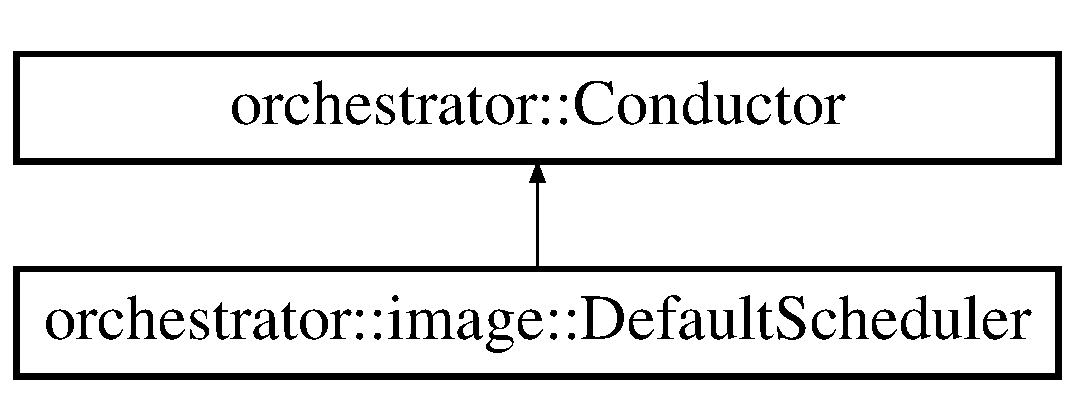
\includegraphics[height=2.000000cm]{dd/d8e/classorchestrator_1_1_conductor}
\end{center}
\end{figure}


The documentation for this class was generated from the following file\+:\begin{DoxyCompactItemize}
\item 
header/orchestrator/Orchestrator.\+h\end{DoxyCompactItemize}

\hypertarget{classhttp_1_1_server_base_1_1_config}{}\section{http\+:\+:Server\+Base$<$ socket\+\_\+type $>$\+:\+:Config Class Reference}
\label{classhttp_1_1_server_base_1_1_config}\index{http\+::\+Server\+Base$<$ socket\+\_\+type $>$\+::\+Config@{http\+::\+Server\+Base$<$ socket\+\_\+type $>$\+::\+Config}}
\subsection*{Public Attributes}
\begin{DoxyCompactItemize}
\item 
\mbox{\Hypertarget{classhttp_1_1_server_base_1_1_config_a2b12945e4b5c9e901e062fda16b1be9c}\label{classhttp_1_1_server_base_1_1_config_a2b12945e4b5c9e901e062fda16b1be9c}} 
unsigned short {\bfseries port}
\item 
std\+::string \hyperlink{classhttp_1_1_server_base_1_1_config_ad0398c9e6bb43163dd91f0bc84854be9}{address}
\item 
\mbox{\Hypertarget{classhttp_1_1_server_base_1_1_config_a7919149e31565fb764794c55a39fd068}\label{classhttp_1_1_server_base_1_1_config_a7919149e31565fb764794c55a39fd068}} 
bool \hyperlink{classhttp_1_1_server_base_1_1_config_a7919149e31565fb764794c55a39fd068}{reuse\+\_\+address}
\begin{DoxyCompactList}\small\item\em Set to false to avoid binding the socket to an address that is already in use. \end{DoxyCompactList}\end{DoxyCompactItemize}
\subsection*{Private Member Functions}
\begin{DoxyCompactItemize}
\item 
\mbox{\Hypertarget{classhttp_1_1_server_base_1_1_config_a313f78f171cc298820ccf40e58ceab34}\label{classhttp_1_1_server_base_1_1_config_a313f78f171cc298820ccf40e58ceab34}} 
{\bfseries Config} (unsigned short port, size\+\_\+t num\+\_\+threads)
\end{DoxyCompactItemize}
\subsection*{Private Attributes}
\begin{DoxyCompactItemize}
\item 
\mbox{\Hypertarget{classhttp_1_1_server_base_1_1_config_a432f55ee3820cebe42afaab349144408}\label{classhttp_1_1_server_base_1_1_config_a432f55ee3820cebe42afaab349144408}} 
size\+\_\+t {\bfseries num\+\_\+threads}
\end{DoxyCompactItemize}
\subsection*{Friends}
\begin{DoxyCompactItemize}
\item 
\mbox{\Hypertarget{classhttp_1_1_server_base_1_1_config_a01d54a7e16ca437c98ec571deca98dfc}\label{classhttp_1_1_server_base_1_1_config_a01d54a7e16ca437c98ec571deca98dfc}} 
class {\bfseries Server\+Base$<$ socket\+\_\+type $>$}
\end{DoxyCompactItemize}


\subsection{Member Data Documentation}
\mbox{\Hypertarget{classhttp_1_1_server_base_1_1_config_ad0398c9e6bb43163dd91f0bc84854be9}\label{classhttp_1_1_server_base_1_1_config_ad0398c9e6bb43163dd91f0bc84854be9}} 
\index{http\+::\+Server\+Base\+::\+Config@{http\+::\+Server\+Base\+::\+Config}!address@{address}}
\index{address@{address}!http\+::\+Server\+Base\+::\+Config@{http\+::\+Server\+Base\+::\+Config}}
\subsubsection{\texorpdfstring{address}{address}}
{\footnotesize\ttfamily template$<$class socket\+\_\+type$>$ \\
std\+::string \hyperlink{classhttp_1_1_server_base}{http\+::\+Server\+Base}$<$ socket\+\_\+type $>$\+::Config\+::address}

I\+Pv4 address in dotted decimal form or I\+Pv6 address in hexadecimal notation. If empty, the address will be any address. 

The documentation for this class was generated from the following file\+:\begin{DoxyCompactItemize}
\item 
header/http/Http\+Server.\+hpp\end{DoxyCompactItemize}

\hypertarget{struct_f_fmpeg_opencv_decoder_1_1config}{}\section{F\+Fmpeg\+Opencv\+Decoder\+:\+:config Struct Reference}
\label{struct_f_fmpeg_opencv_decoder_1_1config}\index{F\+Fmpeg\+Opencv\+Decoder\+::config@{F\+Fmpeg\+Opencv\+Decoder\+::config}}
\subsection*{Public Attributes}
\begin{DoxyCompactItemize}
\item 
\mbox{\Hypertarget{struct_f_fmpeg_opencv_decoder_1_1config_a82c380fa2df2949f0cecbe7bc4b79076}\label{struct_f_fmpeg_opencv_decoder_1_1config_a82c380fa2df2949f0cecbe7bc4b79076}} 
int {\bfseries height}
\item 
\mbox{\Hypertarget{struct_f_fmpeg_opencv_decoder_1_1config_a0230bd2fa59f1c62d25420d8c83a9e82}\label{struct_f_fmpeg_opencv_decoder_1_1config_a0230bd2fa59f1c62d25420d8c83a9e82}} 
int {\bfseries width}
\item 
\mbox{\Hypertarget{struct_f_fmpeg_opencv_decoder_1_1config_a7c92fa819628735fa9a67ae81eaf11c6}\label{struct_f_fmpeg_opencv_decoder_1_1config_a7c92fa819628735fa9a67ae81eaf11c6}} 
int {\bfseries bit\+\_\+rate}
\item 
\mbox{\Hypertarget{struct_f_fmpeg_opencv_decoder_1_1config_a3a3aa7e845b4c812532ff601617cdda7}\label{struct_f_fmpeg_opencv_decoder_1_1config_a3a3aa7e845b4c812532ff601617cdda7}} 
int {\bfseries gop\+\_\+size}
\item 
\mbox{\Hypertarget{struct_f_fmpeg_opencv_decoder_1_1config_acd8aa7a143e0512e58522dc2df9cc7a2}\label{struct_f_fmpeg_opencv_decoder_1_1config_acd8aa7a143e0512e58522dc2df9cc7a2}} 
int {\bfseries fps}
\end{DoxyCompactItemize}


The documentation for this struct was generated from the following file\+:\begin{DoxyCompactItemize}
\item 
header/streaming\+\_\+rtsp/F\+Fmpeg\+Opencv\+Decoder.\+h\end{DoxyCompactItemize}

\hypertarget{classhttp_1_1_config}{}\section{http\+:\+:Config Class Reference}
\label{classhttp_1_1_config}\index{http\+::\+Config@{http\+::\+Config}}
\subsection*{Public Member Functions}
\begin{DoxyCompactItemize}
\item 
\mbox{\Hypertarget{classhttp_1_1_config_a75978d0e657de5df23aa267234500bdd}\label{classhttp_1_1_config_a75978d0e657de5df23aa267234500bdd}} 
{\bfseries Config} (unsigned short port, size\+\_\+t num\+\_\+threads)
\end{DoxyCompactItemize}
\subsection*{Public Attributes}
\begin{DoxyCompactItemize}
\item 
\mbox{\Hypertarget{classhttp_1_1_config_a53fb30a2ad7d7014318156529ce9d2fc}\label{classhttp_1_1_config_a53fb30a2ad7d7014318156529ce9d2fc}} 
size\+\_\+t {\bfseries num\+\_\+threads}
\item 
\mbox{\Hypertarget{classhttp_1_1_config_a814afbe0d0d46ca00ae3849a5b76dd69}\label{classhttp_1_1_config_a814afbe0d0d46ca00ae3849a5b76dd69}} 
unsigned short {\bfseries port}
\item 
std\+::string \hyperlink{classhttp_1_1_config_a2828c9d246da0710621a7bbc26ecab93}{address}
\item 
\mbox{\Hypertarget{classhttp_1_1_config_a2956647487734a4a2c22743bdd898a97}\label{classhttp_1_1_config_a2956647487734a4a2c22743bdd898a97}} 
bool \hyperlink{classhttp_1_1_config_a2956647487734a4a2c22743bdd898a97}{reuse\+\_\+address}
\begin{DoxyCompactList}\small\item\em Set to false to avoid binding the socket to an address that is already in use. \end{DoxyCompactList}\end{DoxyCompactItemize}


\subsection{Member Data Documentation}
\mbox{\Hypertarget{classhttp_1_1_config_a2828c9d246da0710621a7bbc26ecab93}\label{classhttp_1_1_config_a2828c9d246da0710621a7bbc26ecab93}} 
\index{http\+::\+Config@{http\+::\+Config}!address@{address}}
\index{address@{address}!http\+::\+Config@{http\+::\+Config}}
\subsubsection{\texorpdfstring{address}{address}}
{\footnotesize\ttfamily std\+::string http\+::\+Config\+::address}

I\+Pv4 address in dotted decimal form or I\+Pv6 address in hexadecimal notation. If empty, the address will be any address. 

The documentation for this class was generated from the following file\+:\begin{DoxyCompactItemize}
\item 
header/http/Config.\+h\end{DoxyCompactItemize}

\hypertarget{classhttp_1_1_client_base_1_1_config}{}\section{http\+:\+:Client\+Base$<$ socket\+\_\+type $>$\+:\+:Config Class Reference}
\label{classhttp_1_1_client_base_1_1_config}\index{http\+::\+Client\+Base$<$ socket\+\_\+type $>$\+::\+Config@{http\+::\+Client\+Base$<$ socket\+\_\+type $>$\+::\+Config}}
\subsection*{Public Attributes}
\begin{DoxyCompactItemize}
\item 
\mbox{\Hypertarget{classhttp_1_1_client_base_1_1_config_a29fca5b3083e075149d7cc8476d2092b}\label{classhttp_1_1_client_base_1_1_config_a29fca5b3083e075149d7cc8476d2092b}} 
size\+\_\+t \hyperlink{classhttp_1_1_client_base_1_1_config_a29fca5b3083e075149d7cc8476d2092b}{timeout} = 0
\begin{DoxyCompactList}\small\item\em Set timeout on requests in seconds. Default value\+: 0 (no timeout). \end{DoxyCompactList}\item 
\mbox{\Hypertarget{classhttp_1_1_client_base_1_1_config_a607d1a8028e0c5faba269e3a342e830f}\label{classhttp_1_1_client_base_1_1_config_a607d1a8028e0c5faba269e3a342e830f}} 
std\+::string \hyperlink{classhttp_1_1_client_base_1_1_config_a607d1a8028e0c5faba269e3a342e830f}{proxy\+\_\+server}
\begin{DoxyCompactList}\small\item\em Set proxy server (server\+:port) \end{DoxyCompactList}\end{DoxyCompactItemize}
\subsection*{Friends}
\begin{DoxyCompactItemize}
\item 
\mbox{\Hypertarget{classhttp_1_1_client_base_1_1_config_aee5298660229dd276c7169cf7ef3d387}\label{classhttp_1_1_client_base_1_1_config_aee5298660229dd276c7169cf7ef3d387}} 
class {\bfseries Client\+Base$<$ socket\+\_\+type $>$}
\end{DoxyCompactItemize}


The documentation for this class was generated from the following file\+:\begin{DoxyCompactItemize}
\item 
header/http/Http\+Client.\+h\end{DoxyCompactItemize}

\hypertarget{classfilter_1_1data_1_1_connex_data}{}\section{filter\+:\+:data\+:\+:Connex\+Data$<$ Din, Dout $>$ Class Template Reference}
\label{classfilter_1_1data_1_1_connex_data}\index{filter\+::data\+::\+Connex\+Data$<$ Din, Dout $>$@{filter\+::data\+::\+Connex\+Data$<$ Din, Dout $>$}}


The connector is here to connect all data by \hyperlink{classfilter_1_1data_1_1_data_port}{Data\+Port}.  




{\ttfamily \#include $<$Connex\+Data.\+h$>$}

Inheritance diagram for filter\+:\+:data\+:\+:Connex\+Data$<$ Din, Dout $>$\+:\begin{figure}[H]
\begin{center}
\leavevmode
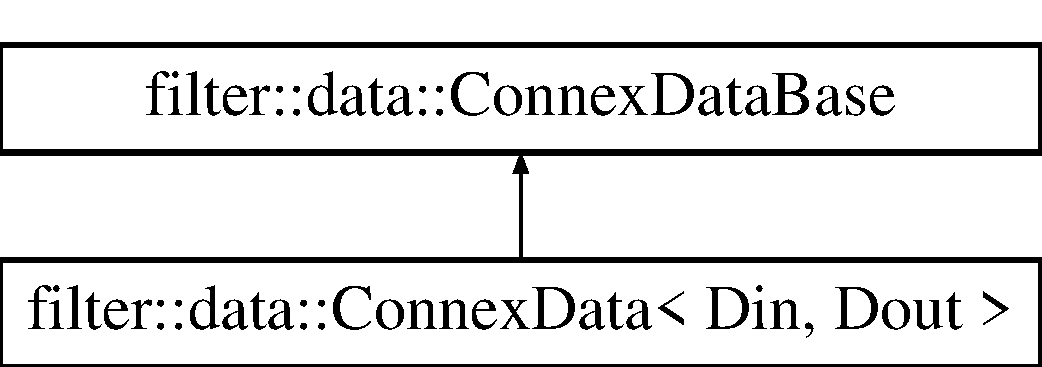
\includegraphics[height=2.000000cm]{dc/d36/classfilter_1_1data_1_1_connex_data}
\end{center}
\end{figure}
\subsection*{Public Member Functions}
\begin{DoxyCompactItemize}
\item 
virtual \hyperlink{classfilter_1_1data_1_1_data_port_base}{Data\+Port\+Base} \& \hyperlink{classfilter_1_1data_1_1_connex_data_aecd47354b992800c9d9e69ad951382fb}{get\+Port} ()
\begin{DoxyCompactList}\small\item\em Get the input port\textquotesingle{}s object. \end{DoxyCompactList}\item 
\mbox{\Hypertarget{classfilter_1_1data_1_1_connex_data_af0e6940e300521b1ecc09c367c8960e2}\label{classfilter_1_1data_1_1_connex_data_af0e6940e300521b1ecc09c367c8960e2}} 
\hyperlink{classfilter_1_1data_1_1_connex_data_af0e6940e300521b1ecc09c367c8960e2}{Connex\+Data} ()
\begin{DoxyCompactList}\small\item\em Default \hyperlink{classfilter_1_1data_1_1_connex_data}{Connex\+Data} constructor. The Way\+Data will be set to I\+N\+D\+A\+TA. \end{DoxyCompactList}\item 
\hyperlink{classfilter_1_1data_1_1_connex_data_a294f855ae8f4b203c8413a32f7e0c692}{Connex\+Data} (Way\+Data way)
\begin{DoxyCompactList}\small\item\em Constructor with a Way\+Data paremeter. The way data is used to tell how the port should handle data. \end{DoxyCompactList}\item 
bool \hyperlink{classfilter_1_1data_1_1_connex_data_a6ae80a4f012442066057ee23dcb6c363}{empty} ()
\begin{DoxyCompactList}\small\item\em Check if the port contains data. \end{DoxyCompactList}\item 
size\+\_\+t \hyperlink{classfilter_1_1data_1_1_connex_data_aed293788ed40932ede5d3a30469f5cfd}{size} ()
\begin{DoxyCompactList}\small\item\em Get the number of stored elements in the port. \end{DoxyCompactList}\item 
Din \hyperlink{classfilter_1_1data_1_1_connex_data_aa7d702b864f00b42b325d2eb6c0a9e91}{get} ()
\begin{DoxyCompactList}\small\item\em Get the port\textquotesingle{}s referenced next data. \end{DoxyCompactList}\item 
Din \hyperlink{classfilter_1_1data_1_1_connex_data_a4367cfe424cefb90470098814a33e326}{pop} ()
\begin{DoxyCompactList}\small\item\em Get the port\textquotesingle{}s referenced next data. If the way is I\+N\+O\+UT, the port will keep a reference to the returned data. In that case modifying the data will affect the one on the port. \end{DoxyCompactList}\item 
{\footnotesize template$<$class Dout\+Broad\+Cast $>$ }\\void \hyperlink{classfilter_1_1data_1_1_connex_data_abd05d79fd08000ff3c92e6fcc8cd41be}{broacast} (Dout\+Broad\+Cast data\+Output)
\begin{DoxyCompactList}\small\item\em \mbox{[}T\+O\+DO\mbox{]} \end{DoxyCompactList}\item 
void \hyperlink{classfilter_1_1data_1_1_connex_data_a16e8347560f6e429a410f21c0b9bd48d}{broacast} (Dout \&data\+Output)
\begin{DoxyCompactList}\small\item\em Broadcat data to the port\textquotesingle{}s output. \end{DoxyCompactList}\item 
void \hyperlink{classfilter_1_1data_1_1_connex_data_a703d8b2465a59a9c8ca79436a1ddfa2b}{push} (Dout data\+Output)
\begin{DoxyCompactList}\small\item\em Send data to the port. The port will establish a link with the next filter of the graph. \end{DoxyCompactList}\item 
{\footnotesize template$<$class indata $>$ }\\void \hyperlink{classfilter_1_1data_1_1_connex_data_af5ed83082314838718aee4fbda767ff9}{push} (indata matrix)
\begin{DoxyCompactList}\small\item\em \mbox{[}T\+O\+DO\mbox{]} \end{DoxyCompactList}\item 
{\footnotesize template$<$class child\+Din , class child\+Dout $>$ }\\void \hyperlink{classfilter_1_1data_1_1_connex_data_a93772066f126cab918b46b285c63073a}{connect\+Output} (\hyperlink{classfilter_1_1data_1_1_connex_data}{Connex\+Data}$<$ child\+Din, child\+Dout $>$ \&connex\+Out)
\begin{DoxyCompactList}\small\item\em Link \hyperlink{classfilter_1_1data_1_1_data_port}{Data\+Port} together to create the data graph. \end{DoxyCompactList}\item 
{\footnotesize template$<$class left\+In , class left\+Out $>$ }\\\hyperlink{classfilter_1_1data_1_1_connex_data}{Connex\+Data}$<$ left\+In, left\+Out $>$ \& \hyperlink{classfilter_1_1data_1_1_connex_data_af7a3a297477db6925728016cb9c8961a}{operator$<$$<$} (\hyperlink{classfilter_1_1data_1_1_connex_data}{Connex\+Data}$<$ left\+In, left\+Out $>$ \&left)
\begin{DoxyCompactList}\small\item\em Link \hyperlink{classfilter_1_1data_1_1_data_port}{Data\+Port} together to create the data graph. \end{DoxyCompactList}\item 
\hyperlink{classfilter_1_1data_1_1_connex_data}{Connex\+Data}$<$ Din, Dout $>$ \& \hyperlink{classfilter_1_1data_1_1_connex_data_a4a4ad046f5772283f520189e62327376}{operator$<$$<$} (\hyperlink{classfilter_1_1data_1_1_connex_data_base}{Connex\+Data\+Base} \&left)
\begin{DoxyCompactList}\small\item\em Link \hyperlink{classfilter_1_1data_1_1_data_port}{Data\+Port} together to create the data graph. \end{DoxyCompactList}\item 
virtual \hyperlink{classfilter_1_1data_1_1_connex_data}{Connex\+Data}$<$ Din, Dout $>$ \& \hyperlink{classfilter_1_1data_1_1_connex_data_a631260c24ddd1050c75a2732081a2d9d}{get\+Cast} ()
\begin{DoxyCompactList}\small\item\em \mbox{[}T\+O\+DO\mbox{]} \end{DoxyCompactList}\end{DoxyCompactItemize}
\subsection*{Public Attributes}
\begin{DoxyCompactItemize}
\item 
\hyperlink{classfilter_1_1data_1_1_data_port}{Data\+Port} \hyperlink{classfilter_1_1data_1_1_connex_data_a607857efe30c0053b56daf6a4da7c83f}{port}
\begin{DoxyCompactList}\small\item\em The Dataport object used to store the input data. \end{DoxyCompactList}\item 
\mbox{\Hypertarget{classfilter_1_1data_1_1_connex_data_aeb46b767ed5e70caa0b1b15aecf1d353}\label{classfilter_1_1data_1_1_connex_data_aeb46b767ed5e70caa0b1b15aecf1d353}} 
std\+::map$<$ \hyperlink{classfilter_1_1data_1_1_connex_data_base}{Connex\+Data\+Base} $\ast$, \hyperlink{classfilter_1_1data_1_1_data_port}{Data\+Port} $\ast$ $>$ \hyperlink{classfilter_1_1data_1_1_connex_data_aeb46b767ed5e70caa0b1b15aecf1d353}{port\+Output}
\begin{DoxyCompactList}\small\item\em \mbox{[}T\+O\+DO\mbox{]} \end{DoxyCompactList}\end{DoxyCompactItemize}
\subsection*{Additional Inherited Members}


\subsection{Detailed Description}
\subsubsection*{template$<$class Din, class Dout$>$\newline
class filter\+::data\+::\+Connex\+Data$<$ Din, Dout $>$}


\begin{DoxyTemplParams}{Template Parameters}
{\em Din} & the Input data type to accept in the I\+Filer Object (comming from parents) \\
\hline
{\em Dout} & the output data type to push to the next data\+Port (going t the childrens) \\
\hline
\end{DoxyTemplParams}


\subsection{Constructor \& Destructor Documentation}
\mbox{\Hypertarget{classfilter_1_1data_1_1_connex_data_a294f855ae8f4b203c8413a32f7e0c692}\label{classfilter_1_1data_1_1_connex_data_a294f855ae8f4b203c8413a32f7e0c692}} 
\index{filter\+::data\+::\+Connex\+Data@{filter\+::data\+::\+Connex\+Data}!Connex\+Data@{Connex\+Data}}
\index{Connex\+Data@{Connex\+Data}!filter\+::data\+::\+Connex\+Data@{filter\+::data\+::\+Connex\+Data}}
\subsubsection{\texorpdfstring{Connex\+Data()}{ConnexData()}}
{\footnotesize\ttfamily template$<$class Din, class Dout$>$ \\
\hyperlink{classfilter_1_1data_1_1_connex_data}{filter\+::data\+::\+Connex\+Data}$<$ Din, Dout $>$\+::\hyperlink{classfilter_1_1data_1_1_connex_data}{Connex\+Data} (\begin{DoxyParamCaption}\item[{Way\+Data}]{way }\end{DoxyParamCaption})\hspace{0.3cm}{\ttfamily [inline]}}


\begin{DoxyParams}{Parameters}
{\em way} & The desired Way\+Data value. \\
\hline
\end{DoxyParams}
\begin{DoxySeeAlso}{See also}
Way\+Data 
\end{DoxySeeAlso}


\subsection{Member Function Documentation}
\mbox{\Hypertarget{classfilter_1_1data_1_1_connex_data_abd05d79fd08000ff3c92e6fcc8cd41be}\label{classfilter_1_1data_1_1_connex_data_abd05d79fd08000ff3c92e6fcc8cd41be}} 
\index{filter\+::data\+::\+Connex\+Data@{filter\+::data\+::\+Connex\+Data}!broacast@{broacast}}
\index{broacast@{broacast}!filter\+::data\+::\+Connex\+Data@{filter\+::data\+::\+Connex\+Data}}
\subsubsection{\texorpdfstring{broacast()}{broacast()}\hspace{0.1cm}{\footnotesize\ttfamily [1/2]}}
{\footnotesize\ttfamily template$<$class Din, class Dout$>$ \\
template$<$class Dout\+Broad\+Cast $>$ \\
void \hyperlink{classfilter_1_1data_1_1_connex_data}{filter\+::data\+::\+Connex\+Data}$<$ Din, Dout $>$\+::broacast (\begin{DoxyParamCaption}\item[{Dout\+Broad\+Cast}]{data\+Output }\end{DoxyParamCaption})\hspace{0.3cm}{\ttfamily [inline]}}


\begin{DoxyTemplParams}{Template Parameters}
{\em Dout\+Broad\+Cast} & \\
\hline
\end{DoxyTemplParams}

\begin{DoxyParams}{Parameters}
{\em data\+Output} & \\
\hline
\end{DoxyParams}
\mbox{\Hypertarget{classfilter_1_1data_1_1_connex_data_a16e8347560f6e429a410f21c0b9bd48d}\label{classfilter_1_1data_1_1_connex_data_a16e8347560f6e429a410f21c0b9bd48d}} 
\index{filter\+::data\+::\+Connex\+Data@{filter\+::data\+::\+Connex\+Data}!broacast@{broacast}}
\index{broacast@{broacast}!filter\+::data\+::\+Connex\+Data@{filter\+::data\+::\+Connex\+Data}}
\subsubsection{\texorpdfstring{broacast()}{broacast()}\hspace{0.1cm}{\footnotesize\ttfamily [2/2]}}
{\footnotesize\ttfamily template$<$class Din, class Dout$>$ \\
void \hyperlink{classfilter_1_1data_1_1_connex_data}{filter\+::data\+::\+Connex\+Data}$<$ Din, Dout $>$\+::broacast (\begin{DoxyParamCaption}\item[{Dout \&}]{data\+Output }\end{DoxyParamCaption})\hspace{0.3cm}{\ttfamily [inline]}}

\mbox{[}T\+O\+DO\mbox{]} 
\begin{DoxyParams}{Parameters}
{\em data\+Output} & The data to broadcast \\
\hline
\end{DoxyParams}
We need to copy the data to avoid to write on image when other children can use it\mbox{\Hypertarget{classfilter_1_1data_1_1_connex_data_a93772066f126cab918b46b285c63073a}\label{classfilter_1_1data_1_1_connex_data_a93772066f126cab918b46b285c63073a}} 
\index{filter\+::data\+::\+Connex\+Data@{filter\+::data\+::\+Connex\+Data}!connect\+Output@{connect\+Output}}
\index{connect\+Output@{connect\+Output}!filter\+::data\+::\+Connex\+Data@{filter\+::data\+::\+Connex\+Data}}
\subsubsection{\texorpdfstring{connect\+Output()}{connectOutput()}}
{\footnotesize\ttfamily template$<$class Din, class Dout$>$ \\
template$<$class child\+Din , class child\+Dout $>$ \\
void \hyperlink{classfilter_1_1data_1_1_connex_data}{filter\+::data\+::\+Connex\+Data}$<$ Din, Dout $>$\+::connect\+Output (\begin{DoxyParamCaption}\item[{\hyperlink{classfilter_1_1data_1_1_connex_data}{Connex\+Data}$<$ child\+Din, child\+Dout $>$ \&}]{connex\+Out }\end{DoxyParamCaption})\hspace{0.3cm}{\ttfamily [inline]}}


\begin{DoxyTemplParams}{Template Parameters}
{\em child\+Din} & the type of the input \\
\hline
{\em child\+Dout} & the type if the output \\
\hline
\end{DoxyTemplParams}

\begin{DoxyParams}{Parameters}
{\em connex\+Out} & the neighboor children where the data port is coming from \\
\hline
\end{DoxyParams}
\mbox{\Hypertarget{classfilter_1_1data_1_1_connex_data_a6ae80a4f012442066057ee23dcb6c363}\label{classfilter_1_1data_1_1_connex_data_a6ae80a4f012442066057ee23dcb6c363}} 
\index{filter\+::data\+::\+Connex\+Data@{filter\+::data\+::\+Connex\+Data}!empty@{empty}}
\index{empty@{empty}!filter\+::data\+::\+Connex\+Data@{filter\+::data\+::\+Connex\+Data}}
\subsubsection{\texorpdfstring{empty()}{empty()}}
{\footnotesize\ttfamily template$<$class Din, class Dout$>$ \\
bool \hyperlink{classfilter_1_1data_1_1_connex_data}{filter\+::data\+::\+Connex\+Data}$<$ Din, Dout $>$\+::empty (\begin{DoxyParamCaption}{ }\end{DoxyParamCaption})\hspace{0.3cm}{\ttfamily [inline]}}

\begin{DoxyReturn}{Returns}
Returns true if there\textquotesingle{}s no data in the port. 
\end{DoxyReturn}
\mbox{\Hypertarget{classfilter_1_1data_1_1_connex_data_aa7d702b864f00b42b325d2eb6c0a9e91}\label{classfilter_1_1data_1_1_connex_data_aa7d702b864f00b42b325d2eb6c0a9e91}} 
\index{filter\+::data\+::\+Connex\+Data@{filter\+::data\+::\+Connex\+Data}!get@{get}}
\index{get@{get}!filter\+::data\+::\+Connex\+Data@{filter\+::data\+::\+Connex\+Data}}
\subsubsection{\texorpdfstring{get()}{get()}}
{\footnotesize\ttfamily template$<$class Din, class Dout$>$ \\
Din \hyperlink{classfilter_1_1data_1_1_connex_data}{filter\+::data\+::\+Connex\+Data}$<$ Din, Dout $>$\+::get (\begin{DoxyParamCaption}{ }\end{DoxyParamCaption})\hspace{0.3cm}{\ttfamily [inline]}}

\begin{DoxyReturn}{Returns}
Returns the port\textquotesingle{}s referenced next data. 
\end{DoxyReturn}
\begin{DoxySeeAlso}{See also}
\hyperlink{classfilter_1_1data_1_1_connex_data_a4367cfe424cefb90470098814a33e326}{pop()} 
\end{DoxySeeAlso}
\mbox{\Hypertarget{classfilter_1_1data_1_1_connex_data_a631260c24ddd1050c75a2732081a2d9d}\label{classfilter_1_1data_1_1_connex_data_a631260c24ddd1050c75a2732081a2d9d}} 
\index{filter\+::data\+::\+Connex\+Data@{filter\+::data\+::\+Connex\+Data}!get\+Cast@{get\+Cast}}
\index{get\+Cast@{get\+Cast}!filter\+::data\+::\+Connex\+Data@{filter\+::data\+::\+Connex\+Data}}
\subsubsection{\texorpdfstring{get\+Cast()}{getCast()}}
{\footnotesize\ttfamily template$<$class Din, class Dout$>$ \\
virtual \hyperlink{classfilter_1_1data_1_1_connex_data}{Connex\+Data}$<$Din, Dout$>$\& \hyperlink{classfilter_1_1data_1_1_connex_data}{filter\+::data\+::\+Connex\+Data}$<$ Din, Dout $>$\+::get\+Cast (\begin{DoxyParamCaption}{ }\end{DoxyParamCaption})\hspace{0.3cm}{\ttfamily [inline]}, {\ttfamily [virtual]}}

\begin{DoxyReturn}{Returns}

\end{DoxyReturn}


Reimplemented from \hyperlink{classfilter_1_1data_1_1_connex_data_base_a7c009f9bb553638dd3a0031a8f04b044}{filter\+::data\+::\+Connex\+Data\+Base}.

\mbox{\Hypertarget{classfilter_1_1data_1_1_connex_data_aecd47354b992800c9d9e69ad951382fb}\label{classfilter_1_1data_1_1_connex_data_aecd47354b992800c9d9e69ad951382fb}} 
\index{filter\+::data\+::\+Connex\+Data@{filter\+::data\+::\+Connex\+Data}!get\+Port@{get\+Port}}
\index{get\+Port@{get\+Port}!filter\+::data\+::\+Connex\+Data@{filter\+::data\+::\+Connex\+Data}}
\subsubsection{\texorpdfstring{get\+Port()}{getPort()}}
{\footnotesize\ttfamily template$<$class Din, class Dout$>$ \\
virtual \hyperlink{classfilter_1_1data_1_1_data_port_base}{Data\+Port\+Base}\& \hyperlink{classfilter_1_1data_1_1_connex_data}{filter\+::data\+::\+Connex\+Data}$<$ Din, Dout $>$\+::get\+Port (\begin{DoxyParamCaption}{ }\end{DoxyParamCaption})\hspace{0.3cm}{\ttfamily [inline]}, {\ttfamily [virtual]}}

\begin{DoxyReturn}{Returns}
Returns a reference to the port 
\end{DoxyReturn}


Reimplemented from \hyperlink{classfilter_1_1data_1_1_connex_data_base_a3cf1336815c061bc721f6b352900e6f4}{filter\+::data\+::\+Connex\+Data\+Base}.

\mbox{\Hypertarget{classfilter_1_1data_1_1_connex_data_af7a3a297477db6925728016cb9c8961a}\label{classfilter_1_1data_1_1_connex_data_af7a3a297477db6925728016cb9c8961a}} 
\index{filter\+::data\+::\+Connex\+Data@{filter\+::data\+::\+Connex\+Data}!operator$<$$<$@{operator$<$$<$}}
\index{operator$<$$<$@{operator$<$$<$}!filter\+::data\+::\+Connex\+Data@{filter\+::data\+::\+Connex\+Data}}
\subsubsection{\texorpdfstring{operator$<$$<$()}{operator<<()}\hspace{0.1cm}{\footnotesize\ttfamily [1/2]}}
{\footnotesize\ttfamily template$<$class Din, class Dout$>$ \\
template$<$class left\+In , class left\+Out $>$ \\
\hyperlink{classfilter_1_1data_1_1_connex_data}{Connex\+Data}$<$left\+In, left\+Out$>$\& \hyperlink{classfilter_1_1data_1_1_connex_data}{filter\+::data\+::\+Connex\+Data}$<$ Din, Dout $>$\+::operator$<$$<$ (\begin{DoxyParamCaption}\item[{\hyperlink{classfilter_1_1data_1_1_connex_data}{Connex\+Data}$<$ left\+In, left\+Out $>$ \&}]{left }\end{DoxyParamCaption})\hspace{0.3cm}{\ttfamily [inline]}}

\mbox{[}T\+O\+DO\mbox{]} 
\begin{DoxyTemplParams}{Template Parameters}
{\em left\+In} & the type of the input \\
\hline
{\em left\+Out} & the type of the output \\
\hline
\end{DoxyTemplParams}

\begin{DoxyParams}{Parameters}
{\em left} & the neighbor children where the data port is coming from \\
\hline
\end{DoxyParams}
\begin{DoxyReturn}{Returns}
A reference to the \hyperlink{classfilter_1_1data_1_1_connex_data}{Connex\+Data} object 
\end{DoxyReturn}
\mbox{\Hypertarget{classfilter_1_1data_1_1_connex_data_a4a4ad046f5772283f520189e62327376}\label{classfilter_1_1data_1_1_connex_data_a4a4ad046f5772283f520189e62327376}} 
\index{filter\+::data\+::\+Connex\+Data@{filter\+::data\+::\+Connex\+Data}!operator$<$$<$@{operator$<$$<$}}
\index{operator$<$$<$@{operator$<$$<$}!filter\+::data\+::\+Connex\+Data@{filter\+::data\+::\+Connex\+Data}}
\subsubsection{\texorpdfstring{operator$<$$<$()}{operator<<()}\hspace{0.1cm}{\footnotesize\ttfamily [2/2]}}
{\footnotesize\ttfamily template$<$class Din, class Dout$>$ \\
\hyperlink{classfilter_1_1data_1_1_connex_data}{Connex\+Data}$<$Din, Dout$>$\& \hyperlink{classfilter_1_1data_1_1_connex_data}{filter\+::data\+::\+Connex\+Data}$<$ Din, Dout $>$\+::operator$<$$<$ (\begin{DoxyParamCaption}\item[{\hyperlink{classfilter_1_1data_1_1_connex_data_base}{Connex\+Data\+Base} \&}]{left }\end{DoxyParamCaption})\hspace{0.3cm}{\ttfamily [inline]}, {\ttfamily [virtual]}}

\mbox{[}T\+O\+DO\mbox{]} 
\begin{DoxyParams}{Parameters}
{\em left} & the neighbor children where the data port is coming from \\
\hline
\end{DoxyParams}
\begin{DoxyReturn}{Returns}
A reference to the \hyperlink{classfilter_1_1data_1_1_connex_data}{Connex\+Data} object 
\end{DoxyReturn}


Reimplemented from \hyperlink{classfilter_1_1data_1_1_connex_data_base_a6d7080cbc59391a6c79ddc12442d6b62}{filter\+::data\+::\+Connex\+Data\+Base}.

\mbox{\Hypertarget{classfilter_1_1data_1_1_connex_data_a4367cfe424cefb90470098814a33e326}\label{classfilter_1_1data_1_1_connex_data_a4367cfe424cefb90470098814a33e326}} 
\index{filter\+::data\+::\+Connex\+Data@{filter\+::data\+::\+Connex\+Data}!pop@{pop}}
\index{pop@{pop}!filter\+::data\+::\+Connex\+Data@{filter\+::data\+::\+Connex\+Data}}
\subsubsection{\texorpdfstring{pop()}{pop()}}
{\footnotesize\ttfamily template$<$class Din, class Dout$>$ \\
Din \hyperlink{classfilter_1_1data_1_1_connex_data}{filter\+::data\+::\+Connex\+Data}$<$ Din, Dout $>$\+::pop (\begin{DoxyParamCaption}{ }\end{DoxyParamCaption})\hspace{0.3cm}{\ttfamily [inline]}}

\begin{DoxyReturn}{Returns}
Returns the port\textquotesingle{}s referenced next data. 
\end{DoxyReturn}
\mbox{\Hypertarget{classfilter_1_1data_1_1_connex_data_a703d8b2465a59a9c8ca79436a1ddfa2b}\label{classfilter_1_1data_1_1_connex_data_a703d8b2465a59a9c8ca79436a1ddfa2b}} 
\index{filter\+::data\+::\+Connex\+Data@{filter\+::data\+::\+Connex\+Data}!push@{push}}
\index{push@{push}!filter\+::data\+::\+Connex\+Data@{filter\+::data\+::\+Connex\+Data}}
\subsubsection{\texorpdfstring{push()}{push()}\hspace{0.1cm}{\footnotesize\ttfamily [1/2]}}
{\footnotesize\ttfamily template$<$class Din, class Dout$>$ \\
void \hyperlink{classfilter_1_1data_1_1_connex_data}{filter\+::data\+::\+Connex\+Data}$<$ Din, Dout $>$\+::push (\begin{DoxyParamCaption}\item[{Dout}]{data\+Output }\end{DoxyParamCaption})\hspace{0.3cm}{\ttfamily [inline]}}


\begin{DoxyParams}{Parameters}
{\em data\+Output} & The data the port should reference \\
\hline
\end{DoxyParams}
\mbox{\Hypertarget{classfilter_1_1data_1_1_connex_data_af5ed83082314838718aee4fbda767ff9}\label{classfilter_1_1data_1_1_connex_data_af5ed83082314838718aee4fbda767ff9}} 
\index{filter\+::data\+::\+Connex\+Data@{filter\+::data\+::\+Connex\+Data}!push@{push}}
\index{push@{push}!filter\+::data\+::\+Connex\+Data@{filter\+::data\+::\+Connex\+Data}}
\subsubsection{\texorpdfstring{push()}{push()}\hspace{0.1cm}{\footnotesize\ttfamily [2/2]}}
{\footnotesize\ttfamily template$<$class Din, class Dout$>$ \\
template$<$class indata $>$ \\
void \hyperlink{classfilter_1_1data_1_1_connex_data}{filter\+::data\+::\+Connex\+Data}$<$ Din, Dout $>$\+::push (\begin{DoxyParamCaption}\item[{indata}]{matrix }\end{DoxyParamCaption})\hspace{0.3cm}{\ttfamily [inline]}}


\begin{DoxyTemplParams}{Template Parameters}
{\em indata} & \\
\hline
\end{DoxyTemplParams}

\begin{DoxyParams}{Parameters}
{\em matrix} & \\
\hline
\end{DoxyParams}
\mbox{\Hypertarget{classfilter_1_1data_1_1_connex_data_aed293788ed40932ede5d3a30469f5cfd}\label{classfilter_1_1data_1_1_connex_data_aed293788ed40932ede5d3a30469f5cfd}} 
\index{filter\+::data\+::\+Connex\+Data@{filter\+::data\+::\+Connex\+Data}!size@{size}}
\index{size@{size}!filter\+::data\+::\+Connex\+Data@{filter\+::data\+::\+Connex\+Data}}
\subsubsection{\texorpdfstring{size()}{size()}}
{\footnotesize\ttfamily template$<$class Din, class Dout$>$ \\
size\+\_\+t \hyperlink{classfilter_1_1data_1_1_connex_data}{filter\+::data\+::\+Connex\+Data}$<$ Din, Dout $>$\+::size (\begin{DoxyParamCaption}{ }\end{DoxyParamCaption})\hspace{0.3cm}{\ttfamily [inline]}}

\begin{DoxyReturn}{Returns}
Returns the number of stored elements in the port 
\end{DoxyReturn}


\subsection{Member Data Documentation}
\mbox{\Hypertarget{classfilter_1_1data_1_1_connex_data_a607857efe30c0053b56daf6a4da7c83f}\label{classfilter_1_1data_1_1_connex_data_a607857efe30c0053b56daf6a4da7c83f}} 
\index{filter\+::data\+::\+Connex\+Data@{filter\+::data\+::\+Connex\+Data}!port@{port}}
\index{port@{port}!filter\+::data\+::\+Connex\+Data@{filter\+::data\+::\+Connex\+Data}}
\subsubsection{\texorpdfstring{port}{port}}
{\footnotesize\ttfamily template$<$class Din, class Dout$>$ \\
\hyperlink{classfilter_1_1data_1_1_data_port}{Data\+Port} \hyperlink{classfilter_1_1data_1_1_connex_data}{filter\+::data\+::\+Connex\+Data}$<$ Din, Dout $>$\+::port}

\begin{DoxySeeAlso}{See also}
\hyperlink{classfilter_1_1data_1_1_data_port}{Data\+Port} 
\end{DoxySeeAlso}


The documentation for this class was generated from the following file\+:\begin{DoxyCompactItemize}
\item 
header/filter/data/Connex\+Data.\+h\end{DoxyCompactItemize}

\hypertarget{classfilter_1_1data_1_1_connex_data_base}{}\section{filter\+:\+:data\+:\+:Connex\+Data\+Base Class Reference}
\label{classfilter_1_1data_1_1_connex_data_base}\index{filter\+::data\+::\+Connex\+Data\+Base@{filter\+::data\+::\+Connex\+Data\+Base}}


The non template class parent for \hyperlink{classfilter_1_1data_1_1_connex_data}{Connex\+Data}. This class is used to contains multiple connector with different type.  




{\ttfamily \#include $<$Connex\+Data.\+h$>$}

Inheritance diagram for filter\+:\+:data\+:\+:Connex\+Data\+Base\+:\begin{figure}[H]
\begin{center}
\leavevmode
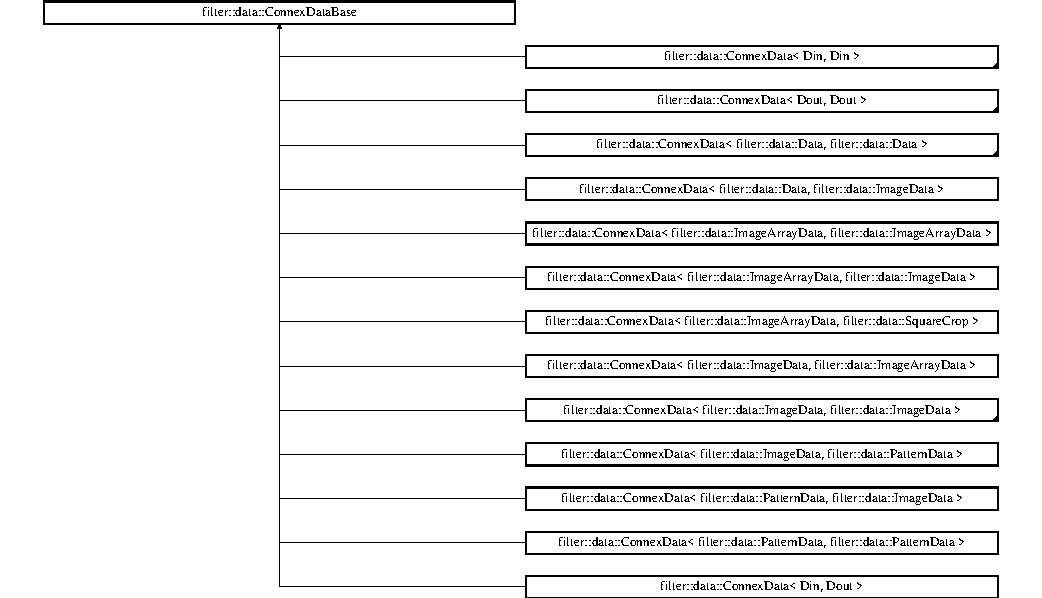
\includegraphics[height=8.016359cm]{da/d49/classfilter_1_1data_1_1_connex_data_base}
\end{center}
\end{figure}
\subsection*{Public Member Functions}
\begin{DoxyCompactItemize}
\item 
\mbox{\Hypertarget{classfilter_1_1data_1_1_connex_data_base_a6b9e22543edbcfa71c7019b693b22806}\label{classfilter_1_1data_1_1_connex_data_base_a6b9e22543edbcfa71c7019b693b22806}} 
{\bfseries Connex\+Data\+Base} (Way\+Data way)
\item 
Way\+Data \hyperlink{classfilter_1_1data_1_1_connex_data_base_a1cfc155ebfbeb5f6a4538a52dafc2e42}{get\+Way} () const
\begin{DoxyCompactList}\small\item\em Get the method how the port handles the data. \end{DoxyCompactList}\item 
virtual \hyperlink{classfilter_1_1data_1_1_connex_data_base}{Connex\+Data\+Base} \& \hyperlink{classfilter_1_1data_1_1_connex_data_base_a7c009f9bb553638dd3a0031a8f04b044}{get\+Cast} ()
\begin{DoxyCompactList}\small\item\em \mbox{[}T\+O\+DO\mbox{]} \end{DoxyCompactList}\item 
virtual \hyperlink{classfilter_1_1data_1_1_connex_data_base}{Connex\+Data\+Base} \& \hyperlink{classfilter_1_1data_1_1_connex_data_base_a6d7080cbc59391a6c79ddc12442d6b62}{operator$<$$<$} (\hyperlink{classfilter_1_1data_1_1_connex_data_base}{Connex\+Data\+Base} \&right)
\begin{DoxyCompactList}\small\item\em \mbox{[}T\+O\+DO\mbox{]} \end{DoxyCompactList}\item 
virtual \hyperlink{classfilter_1_1data_1_1_data_port_base}{Data\+Port\+Base} \& \hyperlink{classfilter_1_1data_1_1_connex_data_base_a3cf1336815c061bc721f6b352900e6f4}{get\+Port} ()
\begin{DoxyCompactList}\small\item\em \mbox{[}T\+O\+DO\mbox{]} \end{DoxyCompactList}\end{DoxyCompactItemize}
\subsection*{Protected Attributes}
\begin{DoxyCompactItemize}
\item 
Way\+Data \hyperlink{classfilter_1_1data_1_1_connex_data_base_a965cbb08a6b61114aa3a66f3254b4f43}{\+\_\+way}
\begin{DoxyCompactList}\small\item\em The Way\+Data field informs how the port should handle the data. \end{DoxyCompactList}\end{DoxyCompactItemize}


\subsection{Member Function Documentation}
\mbox{\Hypertarget{classfilter_1_1data_1_1_connex_data_base_a7c009f9bb553638dd3a0031a8f04b044}\label{classfilter_1_1data_1_1_connex_data_base_a7c009f9bb553638dd3a0031a8f04b044}} 
\index{filter\+::data\+::\+Connex\+Data\+Base@{filter\+::data\+::\+Connex\+Data\+Base}!get\+Cast@{get\+Cast}}
\index{get\+Cast@{get\+Cast}!filter\+::data\+::\+Connex\+Data\+Base@{filter\+::data\+::\+Connex\+Data\+Base}}
\subsubsection{\texorpdfstring{get\+Cast()}{getCast()}}
{\footnotesize\ttfamily virtual \hyperlink{classfilter_1_1data_1_1_connex_data_base}{Connex\+Data\+Base}\& filter\+::data\+::\+Connex\+Data\+Base\+::get\+Cast (\begin{DoxyParamCaption}{ }\end{DoxyParamCaption})\hspace{0.3cm}{\ttfamily [inline]}, {\ttfamily [virtual]}}

\begin{DoxyReturn}{Returns}
\mbox{[}T\+O\+DO\mbox{]} 
\end{DoxyReturn}


Reimplemented in \hyperlink{classfilter_1_1data_1_1_connex_data_a631260c24ddd1050c75a2732081a2d9d}{filter\+::data\+::\+Connex\+Data$<$ Din, Dout $>$}, \hyperlink{classfilter_1_1data_1_1_connex_data_a631260c24ddd1050c75a2732081a2d9d}{filter\+::data\+::\+Connex\+Data$<$ filter\+::data\+::\+Data, filter\+::data\+::\+Data $>$}, \hyperlink{classfilter_1_1data_1_1_connex_data_a631260c24ddd1050c75a2732081a2d9d}{filter\+::data\+::\+Connex\+Data$<$ filter\+::data\+::\+Image\+Data, filter\+::data\+::\+Image\+Array\+Data $>$}, \hyperlink{classfilter_1_1data_1_1_connex_data_a631260c24ddd1050c75a2732081a2d9d}{filter\+::data\+::\+Connex\+Data$<$ filter\+::data\+::\+Pattern\+Data, filter\+::data\+::\+Image\+Data $>$}, \hyperlink{classfilter_1_1data_1_1_connex_data_a631260c24ddd1050c75a2732081a2d9d}{filter\+::data\+::\+Connex\+Data$<$ filter\+::data\+::\+Image\+Data, filter\+::data\+::\+Image\+Data $>$}, \hyperlink{classfilter_1_1data_1_1_connex_data_a631260c24ddd1050c75a2732081a2d9d}{filter\+::data\+::\+Connex\+Data$<$ filter\+::data\+::\+Image\+Data, filter\+::data\+::\+Pattern\+Data $>$}, \hyperlink{classfilter_1_1data_1_1_connex_data_a631260c24ddd1050c75a2732081a2d9d}{filter\+::data\+::\+Connex\+Data$<$ Din, Din $>$}, \hyperlink{classfilter_1_1data_1_1_connex_data_a631260c24ddd1050c75a2732081a2d9d}{filter\+::data\+::\+Connex\+Data$<$ filter\+::data\+::\+Image\+Array\+Data, filter\+::data\+::\+Image\+Data $>$}, \hyperlink{classfilter_1_1data_1_1_connex_data_a631260c24ddd1050c75a2732081a2d9d}{filter\+::data\+::\+Connex\+Data$<$ filter\+::data\+::\+Image\+Array\+Data, filter\+::data\+::\+Image\+Array\+Data $>$}, \hyperlink{classfilter_1_1data_1_1_connex_data_a631260c24ddd1050c75a2732081a2d9d}{filter\+::data\+::\+Connex\+Data$<$ filter\+::data\+::\+Data, filter\+::data\+::\+Image\+Data $>$}, \hyperlink{classfilter_1_1data_1_1_connex_data_a631260c24ddd1050c75a2732081a2d9d}{filter\+::data\+::\+Connex\+Data$<$ Dout, Dout $>$}, \hyperlink{classfilter_1_1data_1_1_connex_data_a631260c24ddd1050c75a2732081a2d9d}{filter\+::data\+::\+Connex\+Data$<$ filter\+::data\+::\+Pattern\+Data, filter\+::data\+::\+Pattern\+Data $>$}, and \hyperlink{classfilter_1_1data_1_1_connex_data_a631260c24ddd1050c75a2732081a2d9d}{filter\+::data\+::\+Connex\+Data$<$ filter\+::data\+::\+Image\+Array\+Data, filter\+::data\+::\+Square\+Crop $>$}.

\mbox{\Hypertarget{classfilter_1_1data_1_1_connex_data_base_a3cf1336815c061bc721f6b352900e6f4}\label{classfilter_1_1data_1_1_connex_data_base_a3cf1336815c061bc721f6b352900e6f4}} 
\index{filter\+::data\+::\+Connex\+Data\+Base@{filter\+::data\+::\+Connex\+Data\+Base}!get\+Port@{get\+Port}}
\index{get\+Port@{get\+Port}!filter\+::data\+::\+Connex\+Data\+Base@{filter\+::data\+::\+Connex\+Data\+Base}}
\subsubsection{\texorpdfstring{get\+Port()}{getPort()}}
{\footnotesize\ttfamily virtual \hyperlink{classfilter_1_1data_1_1_data_port_base}{Data\+Port\+Base}\& filter\+::data\+::\+Connex\+Data\+Base\+::get\+Port (\begin{DoxyParamCaption}{ }\end{DoxyParamCaption})\hspace{0.3cm}{\ttfamily [inline]}, {\ttfamily [virtual]}}

\begin{DoxyReturn}{Returns}

\end{DoxyReturn}


Reimplemented in \hyperlink{classfilter_1_1data_1_1_connex_data_aecd47354b992800c9d9e69ad951382fb}{filter\+::data\+::\+Connex\+Data$<$ Din, Dout $>$}, \hyperlink{classfilter_1_1data_1_1_connex_data_aecd47354b992800c9d9e69ad951382fb}{filter\+::data\+::\+Connex\+Data$<$ filter\+::data\+::\+Data, filter\+::data\+::\+Data $>$}, \hyperlink{classfilter_1_1data_1_1_connex_data_aecd47354b992800c9d9e69ad951382fb}{filter\+::data\+::\+Connex\+Data$<$ filter\+::data\+::\+Image\+Data, filter\+::data\+::\+Image\+Array\+Data $>$}, \hyperlink{classfilter_1_1data_1_1_connex_data_aecd47354b992800c9d9e69ad951382fb}{filter\+::data\+::\+Connex\+Data$<$ filter\+::data\+::\+Pattern\+Data, filter\+::data\+::\+Image\+Data $>$}, \hyperlink{classfilter_1_1data_1_1_connex_data_aecd47354b992800c9d9e69ad951382fb}{filter\+::data\+::\+Connex\+Data$<$ filter\+::data\+::\+Image\+Data, filter\+::data\+::\+Image\+Data $>$}, \hyperlink{classfilter_1_1data_1_1_connex_data_aecd47354b992800c9d9e69ad951382fb}{filter\+::data\+::\+Connex\+Data$<$ filter\+::data\+::\+Image\+Data, filter\+::data\+::\+Pattern\+Data $>$}, \hyperlink{classfilter_1_1data_1_1_connex_data_aecd47354b992800c9d9e69ad951382fb}{filter\+::data\+::\+Connex\+Data$<$ Din, Din $>$}, \hyperlink{classfilter_1_1data_1_1_connex_data_aecd47354b992800c9d9e69ad951382fb}{filter\+::data\+::\+Connex\+Data$<$ filter\+::data\+::\+Image\+Array\+Data, filter\+::data\+::\+Image\+Data $>$}, \hyperlink{classfilter_1_1data_1_1_connex_data_aecd47354b992800c9d9e69ad951382fb}{filter\+::data\+::\+Connex\+Data$<$ filter\+::data\+::\+Image\+Array\+Data, filter\+::data\+::\+Image\+Array\+Data $>$}, \hyperlink{classfilter_1_1data_1_1_connex_data_aecd47354b992800c9d9e69ad951382fb}{filter\+::data\+::\+Connex\+Data$<$ filter\+::data\+::\+Data, filter\+::data\+::\+Image\+Data $>$}, \hyperlink{classfilter_1_1data_1_1_connex_data_aecd47354b992800c9d9e69ad951382fb}{filter\+::data\+::\+Connex\+Data$<$ Dout, Dout $>$}, \hyperlink{classfilter_1_1data_1_1_connex_data_aecd47354b992800c9d9e69ad951382fb}{filter\+::data\+::\+Connex\+Data$<$ filter\+::data\+::\+Pattern\+Data, filter\+::data\+::\+Pattern\+Data $>$}, and \hyperlink{classfilter_1_1data_1_1_connex_data_aecd47354b992800c9d9e69ad951382fb}{filter\+::data\+::\+Connex\+Data$<$ filter\+::data\+::\+Image\+Array\+Data, filter\+::data\+::\+Square\+Crop $>$}.

\mbox{\Hypertarget{classfilter_1_1data_1_1_connex_data_base_a1cfc155ebfbeb5f6a4538a52dafc2e42}\label{classfilter_1_1data_1_1_connex_data_base_a1cfc155ebfbeb5f6a4538a52dafc2e42}} 
\index{filter\+::data\+::\+Connex\+Data\+Base@{filter\+::data\+::\+Connex\+Data\+Base}!get\+Way@{get\+Way}}
\index{get\+Way@{get\+Way}!filter\+::data\+::\+Connex\+Data\+Base@{filter\+::data\+::\+Connex\+Data\+Base}}
\subsubsection{\texorpdfstring{get\+Way()}{getWay()}}
{\footnotesize\ttfamily Way\+Data filter\+::data\+::\+Connex\+Data\+Base\+::get\+Way (\begin{DoxyParamCaption}{ }\end{DoxyParamCaption}) const\hspace{0.3cm}{\ttfamily [inline]}}

\begin{DoxyReturn}{Returns}
Returns the Way\+Data value 
\end{DoxyReturn}
\begin{DoxySeeAlso}{See also}
Way\+Data 
\end{DoxySeeAlso}
\mbox{\Hypertarget{classfilter_1_1data_1_1_connex_data_base_a6d7080cbc59391a6c79ddc12442d6b62}\label{classfilter_1_1data_1_1_connex_data_base_a6d7080cbc59391a6c79ddc12442d6b62}} 
\index{filter\+::data\+::\+Connex\+Data\+Base@{filter\+::data\+::\+Connex\+Data\+Base}!operator$<$$<$@{operator$<$$<$}}
\index{operator$<$$<$@{operator$<$$<$}!filter\+::data\+::\+Connex\+Data\+Base@{filter\+::data\+::\+Connex\+Data\+Base}}
\subsubsection{\texorpdfstring{operator$<$$<$()}{operator<<()}}
{\footnotesize\ttfamily virtual \hyperlink{classfilter_1_1data_1_1_connex_data_base}{Connex\+Data\+Base}\& filter\+::data\+::\+Connex\+Data\+Base\+::operator$<$$<$ (\begin{DoxyParamCaption}\item[{\hyperlink{classfilter_1_1data_1_1_connex_data_base}{Connex\+Data\+Base} \&}]{right }\end{DoxyParamCaption})\hspace{0.3cm}{\ttfamily [inline]}, {\ttfamily [virtual]}}


\begin{DoxyParams}{Parameters}
{\em right} & \\
\hline
\end{DoxyParams}
\begin{DoxyReturn}{Returns}

\end{DoxyReturn}


Reimplemented in \hyperlink{classfilter_1_1data_1_1_connex_data_a4a4ad046f5772283f520189e62327376}{filter\+::data\+::\+Connex\+Data$<$ Din, Dout $>$}, \hyperlink{classfilter_1_1data_1_1_connex_data_a4a4ad046f5772283f520189e62327376}{filter\+::data\+::\+Connex\+Data$<$ filter\+::data\+::\+Data, filter\+::data\+::\+Data $>$}, \hyperlink{classfilter_1_1data_1_1_connex_data_a4a4ad046f5772283f520189e62327376}{filter\+::data\+::\+Connex\+Data$<$ filter\+::data\+::\+Image\+Data, filter\+::data\+::\+Image\+Array\+Data $>$}, \hyperlink{classfilter_1_1data_1_1_connex_data_a4a4ad046f5772283f520189e62327376}{filter\+::data\+::\+Connex\+Data$<$ filter\+::data\+::\+Pattern\+Data, filter\+::data\+::\+Image\+Data $>$}, \hyperlink{classfilter_1_1data_1_1_connex_data_a4a4ad046f5772283f520189e62327376}{filter\+::data\+::\+Connex\+Data$<$ filter\+::data\+::\+Image\+Data, filter\+::data\+::\+Image\+Data $>$}, \hyperlink{classfilter_1_1data_1_1_connex_data_a4a4ad046f5772283f520189e62327376}{filter\+::data\+::\+Connex\+Data$<$ filter\+::data\+::\+Image\+Data, filter\+::data\+::\+Pattern\+Data $>$}, \hyperlink{classfilter_1_1data_1_1_connex_data_a4a4ad046f5772283f520189e62327376}{filter\+::data\+::\+Connex\+Data$<$ Din, Din $>$}, \hyperlink{classfilter_1_1data_1_1_connex_data_a4a4ad046f5772283f520189e62327376}{filter\+::data\+::\+Connex\+Data$<$ filter\+::data\+::\+Image\+Array\+Data, filter\+::data\+::\+Image\+Data $>$}, \hyperlink{classfilter_1_1data_1_1_connex_data_a4a4ad046f5772283f520189e62327376}{filter\+::data\+::\+Connex\+Data$<$ filter\+::data\+::\+Image\+Array\+Data, filter\+::data\+::\+Image\+Array\+Data $>$}, \hyperlink{classfilter_1_1data_1_1_connex_data_a4a4ad046f5772283f520189e62327376}{filter\+::data\+::\+Connex\+Data$<$ filter\+::data\+::\+Data, filter\+::data\+::\+Image\+Data $>$}, \hyperlink{classfilter_1_1data_1_1_connex_data_a4a4ad046f5772283f520189e62327376}{filter\+::data\+::\+Connex\+Data$<$ Dout, Dout $>$}, \hyperlink{classfilter_1_1data_1_1_connex_data_a4a4ad046f5772283f520189e62327376}{filter\+::data\+::\+Connex\+Data$<$ filter\+::data\+::\+Pattern\+Data, filter\+::data\+::\+Pattern\+Data $>$}, and \hyperlink{classfilter_1_1data_1_1_connex_data_a4a4ad046f5772283f520189e62327376}{filter\+::data\+::\+Connex\+Data$<$ filter\+::data\+::\+Image\+Array\+Data, filter\+::data\+::\+Square\+Crop $>$}.



\subsection{Member Data Documentation}
\mbox{\Hypertarget{classfilter_1_1data_1_1_connex_data_base_a965cbb08a6b61114aa3a66f3254b4f43}\label{classfilter_1_1data_1_1_connex_data_base_a965cbb08a6b61114aa3a66f3254b4f43}} 
\index{filter\+::data\+::\+Connex\+Data\+Base@{filter\+::data\+::\+Connex\+Data\+Base}!\+\_\+way@{\+\_\+way}}
\index{\+\_\+way@{\+\_\+way}!filter\+::data\+::\+Connex\+Data\+Base@{filter\+::data\+::\+Connex\+Data\+Base}}
\subsubsection{\texorpdfstring{\+\_\+way}{\_way}}
{\footnotesize\ttfamily Way\+Data filter\+::data\+::\+Connex\+Data\+Base\+::\+\_\+way\hspace{0.3cm}{\ttfamily [protected]}}

\begin{DoxySeeAlso}{See also}
Way\+Data 
\end{DoxySeeAlso}


The documentation for this class was generated from the following file\+:\begin{DoxyCompactItemize}
\item 
header/filter/data/Connex\+Data.\+h\end{DoxyCompactItemize}

\hypertarget{classfilter_1_1data_1_1_connex_input}{}\section{filter\+:\+:data\+:\+:Connex\+Input$<$ Din $>$ Class Template Reference}
\label{classfilter_1_1data_1_1_connex_input}\index{filter\+::data\+::\+Connex\+Input$<$ Din $>$@{filter\+::data\+::\+Connex\+Input$<$ Din $>$}}


A derived class of of \hyperlink{classfilter_1_1data_1_1_connex_data}{Connex\+Data}. It\textquotesingle{}s a specialization to restrict the object to an input connector there is only one port connexion.  




{\ttfamily \#include $<$Connex\+Data.\+h$>$}

Inheritance diagram for filter\+:\+:data\+:\+:Connex\+Input$<$ Din $>$\+:\begin{figure}[H]
\begin{center}
\leavevmode
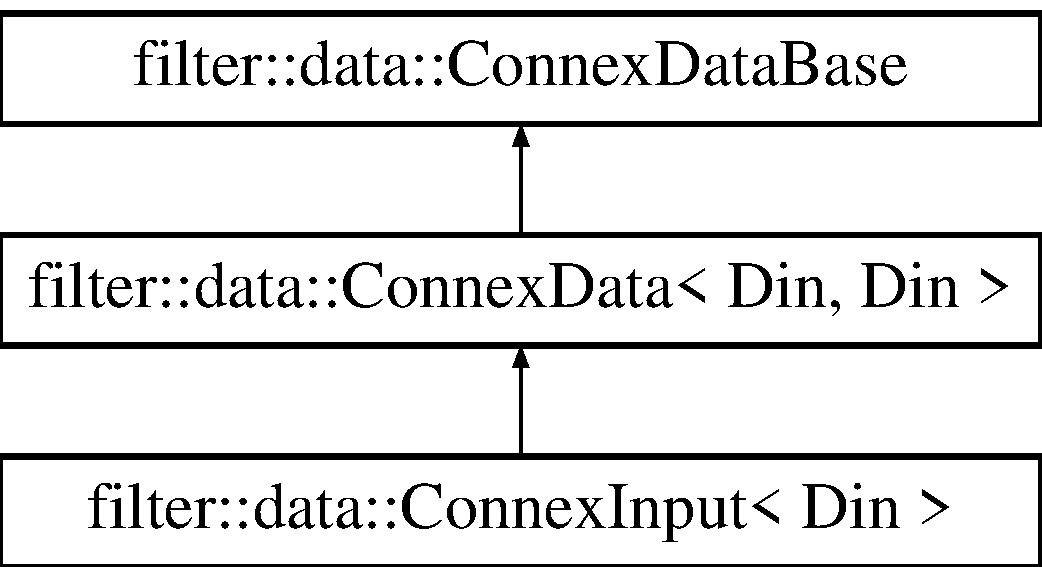
\includegraphics[height=3.000000cm]{df/ddc/classfilter_1_1data_1_1_connex_input}
\end{center}
\end{figure}
\subsection*{Public Member Functions}
\begin{DoxyCompactItemize}
\item 
\mbox{\Hypertarget{classfilter_1_1data_1_1_connex_input_a5c7e7ee73508eab04151a486ca86d32a}\label{classfilter_1_1data_1_1_connex_input_a5c7e7ee73508eab04151a486ca86d32a}} 
{\bfseries Connex\+Input} (Din $\ast$data, Way\+Data \&way)
\item 
\mbox{\Hypertarget{classfilter_1_1data_1_1_connex_input_a17efe16aab1f8715975e56f99212841a}\label{classfilter_1_1data_1_1_connex_input_a17efe16aab1f8715975e56f99212841a}} 
void {\bfseries push} (Din \&data\+Output)
\item 
\mbox{\Hypertarget{classfilter_1_1data_1_1_connex_input_a2ed43bbc4b698728aab5feef012b922d}\label{classfilter_1_1data_1_1_connex_input_a2ed43bbc4b698728aab5feef012b922d}} 
{\footnotesize template$<$class indata $>$ }\\void {\bfseries push} (indata matrix)
\item 
\mbox{\Hypertarget{classfilter_1_1data_1_1_connex_input_aa0851447c5a5d7347fbdde287e8f6db1}\label{classfilter_1_1data_1_1_connex_input_aa0851447c5a5d7347fbdde287e8f6db1}} 
void {\bfseries connect\+Input} (\hyperlink{classfilter_1_1data_1_1_connex_data}{Connex\+Data}$<$ Din, Din $>$ \&connex\+In)
\item 
\mbox{\Hypertarget{classfilter_1_1data_1_1_connex_input_ad2973cd9259580e910a3369525ab896b}\label{classfilter_1_1data_1_1_connex_input_ad2973cd9259580e910a3369525ab896b}} 
void {\bfseries forward\+Data} ()
\end{DoxyCompactItemize}
\subsection*{Additional Inherited Members}


\subsection{Detailed Description}
\subsubsection*{template$<$class Din$>$\newline
class filter\+::data\+::\+Connex\+Input$<$ Din $>$}


\begin{DoxyTemplParams}{Template Parameters}
{\em Din} & the data type to send to children \\
\hline
\end{DoxyTemplParams}


The documentation for this class was generated from the following file\+:\begin{DoxyCompactItemize}
\item 
header/filter/data/Connex\+Data.\+h\end{DoxyCompactItemize}

\hypertarget{classfilter_1_1data_1_1_connex_output}{}\section{filter\+:\+:data\+:\+:Connex\+Output$<$ Dout $>$ Class Template Reference}
\label{classfilter_1_1data_1_1_connex_output}\index{filter\+::data\+::\+Connex\+Output$<$ Dout $>$@{filter\+::data\+::\+Connex\+Output$<$ Dout $>$}}


A derived class of of \hyperlink{classfilter_1_1data_1_1_connex_data}{Connex\+Data}. It\textquotesingle{}s a specialization to restrict the object to an output connector there is only one port connexion.  




{\ttfamily \#include $<$Connex\+Data.\+h$>$}

Inheritance diagram for filter\+:\+:data\+:\+:Connex\+Output$<$ Dout $>$\+:\begin{figure}[H]
\begin{center}
\leavevmode
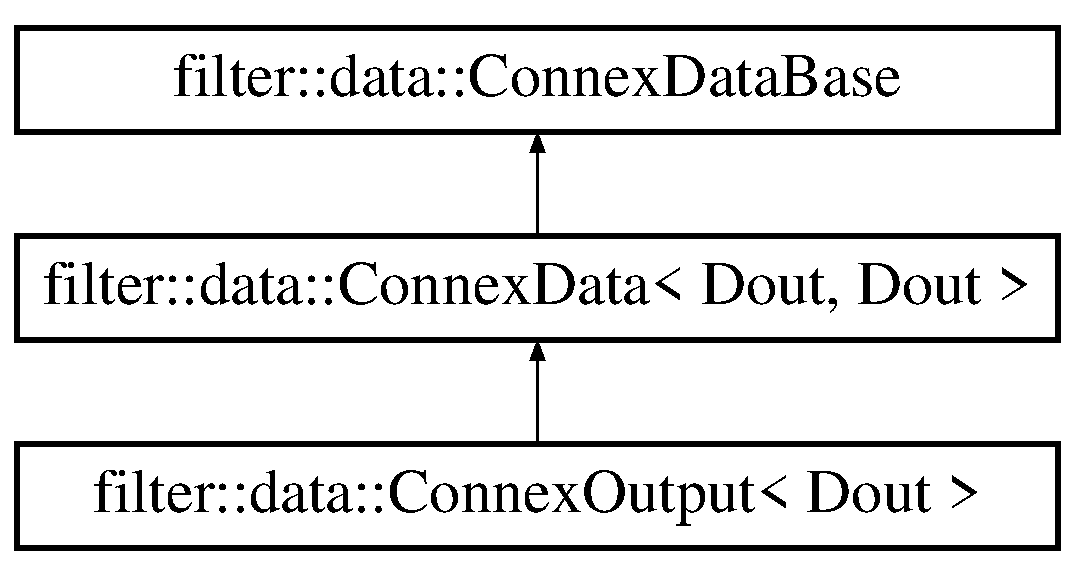
\includegraphics[height=3.000000cm]{d6/ddc/classfilter_1_1data_1_1_connex_output}
\end{center}
\end{figure}
\subsection*{Public Member Functions}
\begin{DoxyCompactItemize}
\item 
\mbox{\Hypertarget{classfilter_1_1data_1_1_connex_output_a343d811aad79aff050e4e2e0a97d0a53}\label{classfilter_1_1data_1_1_connex_output_a343d811aad79aff050e4e2e0a97d0a53}} 
Dout {\bfseries pop} ()
\item 
\mbox{\Hypertarget{classfilter_1_1data_1_1_connex_output_ac0cfae1835db1de96a59678551f29f8c}\label{classfilter_1_1data_1_1_connex_output_ac0cfae1835db1de96a59678551f29f8c}} 
void {\bfseries Connect\+Output} (\hyperlink{classfilter_1_1data_1_1_connex_data}{Connex\+Data}$<$ Dout, Dout $>$ \&connex\+In)
\end{DoxyCompactItemize}
\subsection*{Additional Inherited Members}


\subsection{Detailed Description}
\subsubsection*{template$<$class Dout$>$\newline
class filter\+::data\+::\+Connex\+Output$<$ Dout $>$}


\begin{DoxyTemplParams}{Template Parameters}
{\em Dout} & the data type to receive from parent \\
\hline
\end{DoxyTemplParams}


The documentation for this class was generated from the following file\+:\begin{DoxyCompactItemize}
\item 
header/filter/data/Connex\+Data.\+h\end{DoxyCompactItemize}

\hypertarget{classhttp_1_1_server_base_1_1_content}{}\section{http\+:\+:Server\+Base$<$ socket\+\_\+type $>$\+:\+:Content Class Reference}
\label{classhttp_1_1_server_base_1_1_content}\index{http\+::\+Server\+Base$<$ socket\+\_\+type $>$\+::\+Content@{http\+::\+Server\+Base$<$ socket\+\_\+type $>$\+::\+Content}}
Inheritance diagram for http\+:\+:Server\+Base$<$ socket\+\_\+type $>$\+:\+:Content\+:\begin{figure}[H]
\begin{center}
\leavevmode
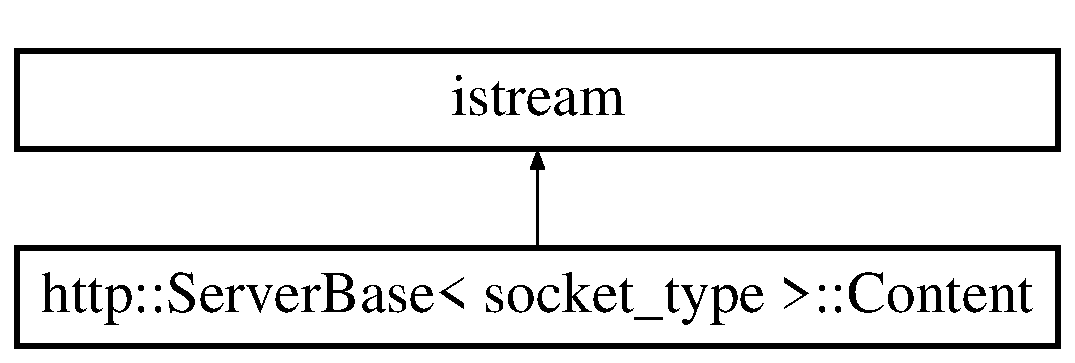
\includegraphics[height=2.000000cm]{d8/d54/classhttp_1_1_server_base_1_1_content}
\end{center}
\end{figure}
\subsection*{Public Member Functions}
\begin{DoxyCompactItemize}
\item 
\mbox{\Hypertarget{classhttp_1_1_server_base_1_1_content_a474902c6c394af6697cf6de4bd245335}\label{classhttp_1_1_server_base_1_1_content_a474902c6c394af6697cf6de4bd245335}} 
size\+\_\+t {\bfseries size} ()
\item 
\mbox{\Hypertarget{classhttp_1_1_server_base_1_1_content_ac91ebb89641f6aefaf0a75c6c7cd1ddf}\label{classhttp_1_1_server_base_1_1_content_ac91ebb89641f6aefaf0a75c6c7cd1ddf}} 
std\+::string {\bfseries string} ()
\item 
\mbox{\Hypertarget{classhttp_1_1_server_base_1_1_content_a0a5b6c2e1ca0a8d03e6fa6078e9781c3}\label{classhttp_1_1_server_base_1_1_content_a0a5b6c2e1ca0a8d03e6fa6078e9781c3}} 
{\bfseries Content} (boost\+::asio\+::streambuf \&streambuf)
\end{DoxyCompactItemize}
\subsection*{Public Attributes}
\begin{DoxyCompactItemize}
\item 
\mbox{\Hypertarget{classhttp_1_1_server_base_1_1_content_a35706768de83012d6faac164a3653672}\label{classhttp_1_1_server_base_1_1_content_a35706768de83012d6faac164a3653672}} 
boost\+::asio\+::streambuf \& {\bfseries streambuf}
\end{DoxyCompactItemize}
\subsection*{Friends}
\begin{DoxyCompactItemize}
\item 
\mbox{\Hypertarget{classhttp_1_1_server_base_1_1_content_a01d54a7e16ca437c98ec571deca98dfc}\label{classhttp_1_1_server_base_1_1_content_a01d54a7e16ca437c98ec571deca98dfc}} 
class {\bfseries Server\+Base$<$ socket\+\_\+type $>$}
\end{DoxyCompactItemize}


The documentation for this class was generated from the following file\+:\begin{DoxyCompactItemize}
\item 
header/http/Http\+Server.\+hpp\end{DoxyCompactItemize}

\hypertarget{classhttp_1_1_content}{}\section{http\+:\+:Content Class Reference}
\label{classhttp_1_1_content}\index{http\+::\+Content@{http\+::\+Content}}
Inheritance diagram for http\+:\+:Content\+:\begin{figure}[H]
\begin{center}
\leavevmode
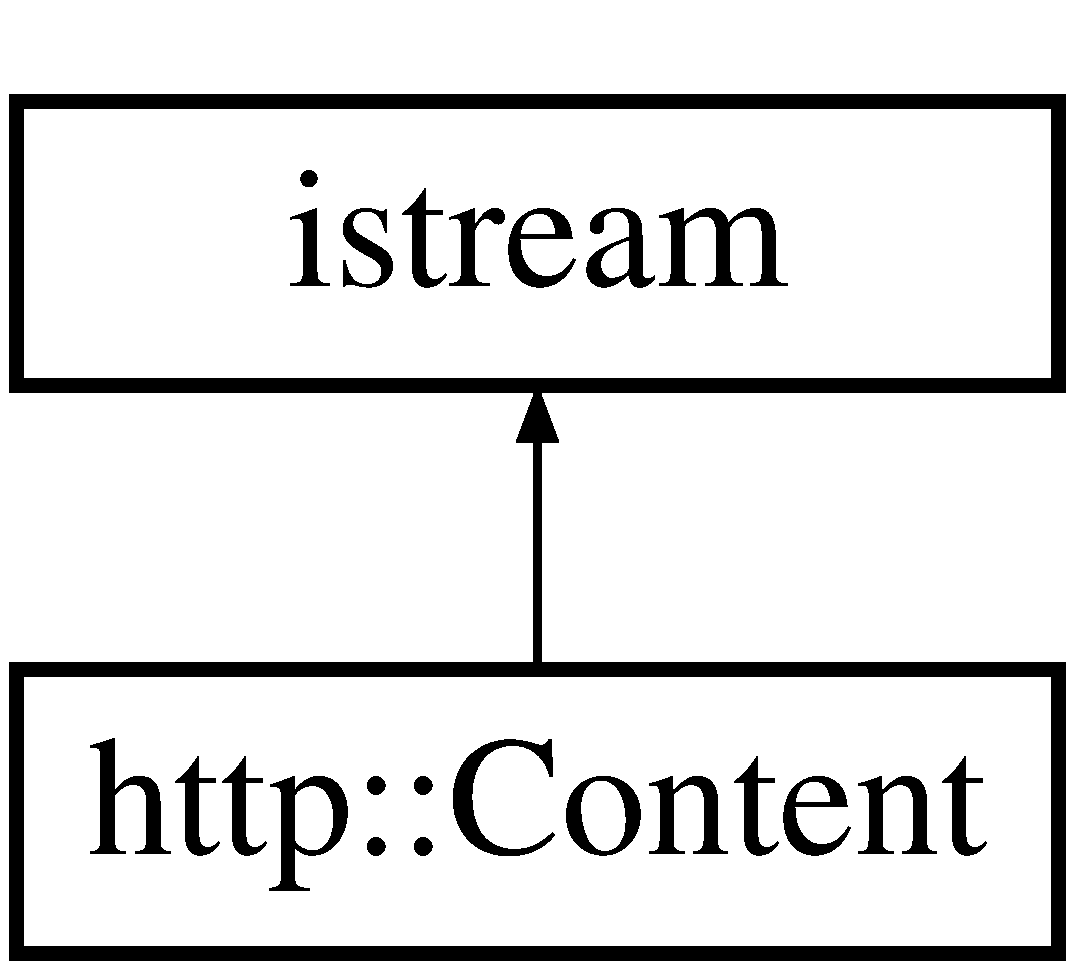
\includegraphics[height=2.000000cm]{dd/d5f/classhttp_1_1_content}
\end{center}
\end{figure}
\subsection*{Public Member Functions}
\begin{DoxyCompactItemize}
\item 
\mbox{\Hypertarget{classhttp_1_1_content_a5a39199b9f8c05ac3c7a4088ee255c5f}\label{classhttp_1_1_content_a5a39199b9f8c05ac3c7a4088ee255c5f}} 
size\+\_\+t {\bfseries size} ()
\item 
\mbox{\Hypertarget{classhttp_1_1_content_af57d45e4b9f4ea12e238a0b9cf7e23e5}\label{classhttp_1_1_content_af57d45e4b9f4ea12e238a0b9cf7e23e5}} 
std\+::string {\bfseries string} ()
\item 
\mbox{\Hypertarget{classhttp_1_1_content_a6e7c7b674b76873a64afe380cb0dd11a}\label{classhttp_1_1_content_a6e7c7b674b76873a64afe380cb0dd11a}} 
{\bfseries Content} (boost\+::asio\+::streambuf \&streambuf)
\end{DoxyCompactItemize}
\subsection*{Public Attributes}
\begin{DoxyCompactItemize}
\item 
\mbox{\Hypertarget{classhttp_1_1_content_a0157e071440455dc1a0f59e1f0824b70}\label{classhttp_1_1_content_a0157e071440455dc1a0f59e1f0824b70}} 
boost\+::asio\+::streambuf \& {\bfseries streambuf}
\end{DoxyCompactItemize}


The documentation for this class was generated from the following file\+:\begin{DoxyCompactItemize}
\item 
header/http/Content.\+h\end{DoxyCompactItemize}

\hypertarget{classfilter_1_1algos_1_1_contrast}{}\section{filter\+:\+:algos\+:\+:Contrast Class Reference}
\label{classfilter_1_1algos_1_1_contrast}\index{filter\+::algos\+::\+Contrast@{filter\+::algos\+::\+Contrast}}
Inheritance diagram for filter\+:\+:algos\+:\+:Contrast\+:\begin{figure}[H]
\begin{center}
\leavevmode
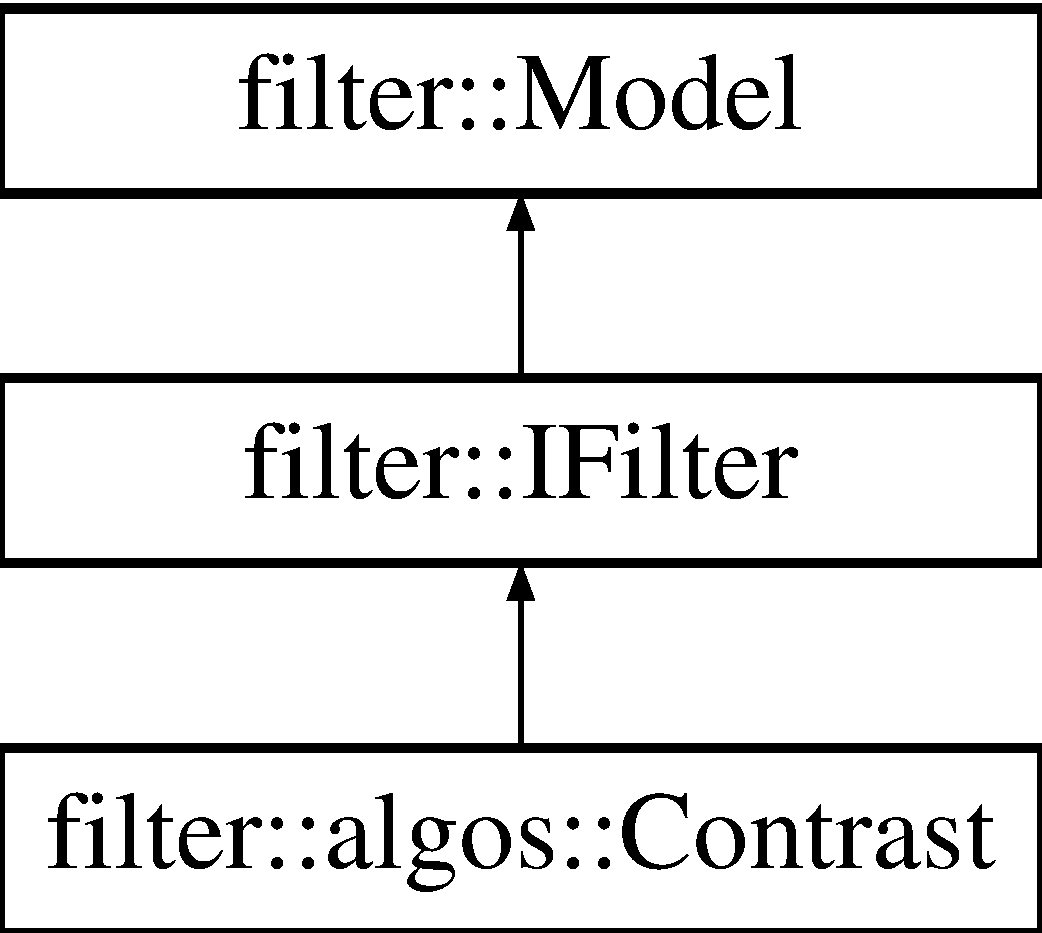
\includegraphics[height=3.000000cm]{d8/d7f/classfilter_1_1algos_1_1_contrast}
\end{center}
\end{figure}
\subsection*{Public Types}
\begin{DoxyCompactItemize}
\item 
\mbox{\Hypertarget{classfilter_1_1algos_1_1_contrast_a8f10e6b1f878a4e3c7fd932617099fc5}\label{classfilter_1_1algos_1_1_contrast_a8f10e6b1f878a4e3c7fd932617099fc5}} 
typedef \hyperlink{class_proxy_functor}{Proxy\+Functor}$<$ \hyperlink{classfilter_1_1algos_1_1_contrast}{Contrast} $>$ {\bfseries \+\_\+proxy\+Functor}
\item 
\mbox{\Hypertarget{classfilter_1_1algos_1_1_contrast_aee7b92121d7d92aac068510ca1926d15}\label{classfilter_1_1algos_1_1_contrast_aee7b92121d7d92aac068510ca1926d15}} 
typedef \hyperlink{classfilter_1_1algos_1_1_contrast}{Contrast} {\bfseries mytype}
\item 
\mbox{\Hypertarget{classfilter_1_1algos_1_1_contrast_ad98354d1bb5d645be6ad7f65bebfbcec}\label{classfilter_1_1algos_1_1_contrast_ad98354d1bb5d645be6ad7f65bebfbcec}} 
typedef char {\bfseries vartype\+\_\+\+\_\+unused}
\end{DoxyCompactItemize}
\subsection*{Public Member Functions}
\begin{DoxyCompactItemize}
\item 
\mbox{\Hypertarget{classfilter_1_1algos_1_1_contrast_a43d7bd15c17760f14f8086fe9b2dd38a}\label{classfilter_1_1algos_1_1_contrast_a43d7bd15c17760f14f8086fe9b2dd38a}} 
void {\bfseries set\+\_\+unused\+\_\+from\+\_\+json} (boost\+::property\+\_\+tree\+::ptree \&json\+Class)
\item 
\mbox{\Hypertarget{classfilter_1_1algos_1_1_contrast_a0654aa2555f283ea0e16f901e2192dec}\label{classfilter_1_1algos_1_1_contrast_a0654aa2555f283ea0e16f901e2192dec}} 
void {\bfseries set\+\_\+unused} (vartype\+\_\+\+\_\+unused \&\+\_\+\+\_\+unused)
\item 
\mbox{\Hypertarget{classfilter_1_1algos_1_1_contrast_a509c33e0fc49feef938317e9ac2eb5f2}\label{classfilter_1_1algos_1_1_contrast_a509c33e0fc49feef938317e9ac2eb5f2}} 
vartype\+\_\+\+\_\+unused {\bfseries get\+\_\+unused} ()
\item 
\mbox{\Hypertarget{classfilter_1_1algos_1_1_contrast_a94e8234022e5cf794bf7c707193624f2}\label{classfilter_1_1algos_1_1_contrast_a94e8234022e5cf794bf7c707193624f2}} 
void {\bfseries copy\+\_\+unused} (\hyperlink{classfilter_1_1algos_1_1_contrast}{mytype} $\ast$instance)
\item 
\mbox{\Hypertarget{classfilter_1_1algos_1_1_contrast_ae92784fa32e5ea5fcceb804551189789}\label{classfilter_1_1algos_1_1_contrast_ae92784fa32e5ea5fcceb804551189789}} 
Hipe\+Status {\bfseries process} () override
\end{DoxyCompactItemize}
\subsection*{Public Attributes}
\begin{DoxyCompactItemize}
\item 
\mbox{\Hypertarget{classfilter_1_1algos_1_1_contrast_af45a20ffb1d8182950c6058860877968}\label{classfilter_1_1algos_1_1_contrast_af45a20ffb1d8182950c6058860877968}} 
char {\bfseries unused}
\end{DoxyCompactItemize}
\subsection*{Private Member Functions}
\begin{DoxyCompactItemize}
\item 
\mbox{\Hypertarget{classfilter_1_1algos_1_1_contrast_aa2abbe606016c6a581fd42515caed2d8}\label{classfilter_1_1algos_1_1_contrast_aa2abbe606016c6a581fd42515caed2d8}} 
virtual \hyperlink{classfilter_1_1data_1_1_connex_data_base}{data\+::\+Connex\+Data\+Base} \& {\bfseries get\+Connector} ()
\end{DoxyCompactItemize}
\subsection*{Private Attributes}
\begin{DoxyCompactItemize}
\item 
\mbox{\Hypertarget{classfilter_1_1algos_1_1_contrast_afe0214066718eb141d3b7e6417a3f7ca}\label{classfilter_1_1algos_1_1_contrast_afe0214066718eb141d3b7e6417a3f7ca}} 
\hyperlink{classfilter_1_1data_1_1_connex_data}{data\+::\+Connex\+Data}$<$ \hyperlink{classfilter_1_1data_1_1_image_data}{data\+::\+Image\+Data}, \hyperlink{classfilter_1_1data_1_1_image_data}{data\+::\+Image\+Data} $>$ {\bfseries \+\_\+connex\+Data}
\end{DoxyCompactItemize}
\subsection*{Additional Inherited Members}


The documentation for this class was generated from the following file\+:\begin{DoxyCompactItemize}
\item 
header/filter/\+Algos/Contrast.\+h\end{DoxyCompactItemize}

\hypertarget{classfilter_1_1data_1_1_copy_object}{}\section{filter\+:\+:data\+:\+:Copy\+Object$<$ My\+Class $>$ Class Template Reference}
\label{classfilter_1_1data_1_1_copy_object}\index{filter\+::data\+::\+Copy\+Object$<$ My\+Class $>$@{filter\+::data\+::\+Copy\+Object$<$ My\+Class $>$}}
\subsection*{Public Member Functions}
\begin{DoxyCompactItemize}
\item 
\mbox{\Hypertarget{classfilter_1_1data_1_1_copy_object_a8c66b211a6a1b5bdc8cab5a7855cbf33}\label{classfilter_1_1data_1_1_copy_object_a8c66b211a6a1b5bdc8cab5a7855cbf33}} 
{\footnotesize template$<$$>$ }\\double $\ast$ {\bfseries copy} (double $\ast$\&left)
\end{DoxyCompactItemize}
\subsection*{Static Public Member Functions}
\begin{DoxyCompactItemize}
\item 
\mbox{\Hypertarget{classfilter_1_1data_1_1_copy_object_ad24997fa56580b4a999e5baa9e42e3b6}\label{classfilter_1_1data_1_1_copy_object_ad24997fa56580b4a999e5baa9e42e3b6}} 
static My\+Class {\bfseries copy} (My\+Class \&left)
\end{DoxyCompactItemize}


The documentation for this class was generated from the following file\+:\begin{DoxyCompactItemize}
\item 
header/filter/data/Connex\+Data.\+h\end{DoxyCompactItemize}

\hypertarget{classfilter_1_1_algos_1_1_crop}{}\section{filter\+:\+:Algos\+:\+:Crop Class Reference}
\label{classfilter_1_1_algos_1_1_crop}\index{filter\+::\+Algos\+::\+Crop@{filter\+::\+Algos\+::\+Crop}}


The \hyperlink{classfilter_1_1_algos_1_1_crop}{Crop} filter will let the user manually select (with mouse input) a region of interest in an image.  




{\ttfamily \#include $<$Crop.\+h$>$}

Inheritance diagram for filter\+:\+:Algos\+:\+:Crop\+:\begin{figure}[H]
\begin{center}
\leavevmode
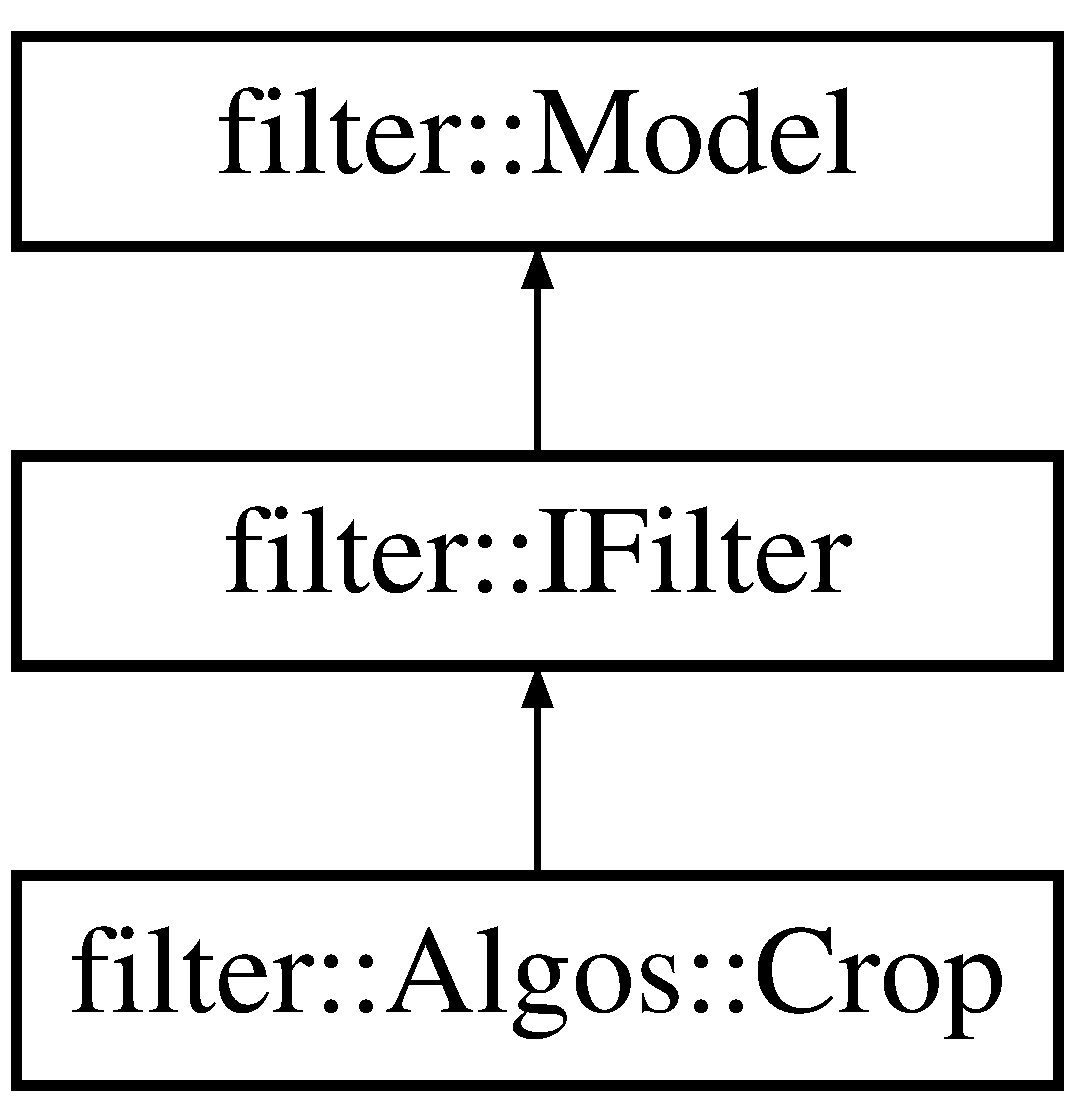
\includegraphics[height=3.000000cm]{dd/d88/classfilter_1_1_algos_1_1_crop}
\end{center}
\end{figure}
\subsection*{Public Types}
\begin{DoxyCompactItemize}
\item 
\mbox{\Hypertarget{classfilter_1_1_algos_1_1_crop_a95541eb3cc7f5595ce7730724fd2c6b5}\label{classfilter_1_1_algos_1_1_crop_a95541eb3cc7f5595ce7730724fd2c6b5}} 
typedef \hyperlink{class_proxy_functor}{Proxy\+Functor}$<$ \hyperlink{classfilter_1_1_algos_1_1_crop}{Crop} $>$ {\bfseries \+\_\+proxy\+Functor}
\item 
\mbox{\Hypertarget{classfilter_1_1_algos_1_1_crop_ab0d7dad1833eb9f0ad2aa7ac7c4a950d}\label{classfilter_1_1_algos_1_1_crop_ab0d7dad1833eb9f0ad2aa7ac7c4a950d}} 
typedef \hyperlink{classfilter_1_1_algos_1_1_crop}{Crop} {\bfseries mytype}
\item 
\mbox{\Hypertarget{classfilter_1_1_algos_1_1_crop_add9101538c1824755b8a57ee7e63b699}\label{classfilter_1_1_algos_1_1_crop_add9101538c1824755b8a57ee7e63b699}} 
typedef float {\bfseries vartype\+\_\+\+\_\+unused\+\_\+parameter}
\end{DoxyCompactItemize}
\subsection*{Public Member Functions}
\begin{DoxyCompactItemize}
\item 
\mbox{\Hypertarget{classfilter_1_1_algos_1_1_crop_ae36f5682bec6d851ddd0a65de6066ff3}\label{classfilter_1_1_algos_1_1_crop_ae36f5682bec6d851ddd0a65de6066ff3}} 
void {\bfseries set\+\_\+unused\+\_\+parameter\+\_\+from\+\_\+json} (boost\+::property\+\_\+tree\+::ptree \&json\+Class)
\item 
\mbox{\Hypertarget{classfilter_1_1_algos_1_1_crop_abe8021a27f7a36822858d0ed3c83aeb8}\label{classfilter_1_1_algos_1_1_crop_abe8021a27f7a36822858d0ed3c83aeb8}} 
void {\bfseries set\+\_\+unused\+\_\+parameter} (vartype\+\_\+\+\_\+unused\+\_\+parameter \&\+\_\+\+\_\+unused\+\_\+parameter)
\item 
\mbox{\Hypertarget{classfilter_1_1_algos_1_1_crop_ae4d3c8e6fc650f5dff23482ba40a2779}\label{classfilter_1_1_algos_1_1_crop_ae4d3c8e6fc650f5dff23482ba40a2779}} 
vartype\+\_\+\+\_\+unused\+\_\+parameter {\bfseries get\+\_\+unused\+\_\+parameter} ()
\item 
\mbox{\Hypertarget{classfilter_1_1_algos_1_1_crop_a81705a3d09c4ae88141dea27809d887f}\label{classfilter_1_1_algos_1_1_crop_a81705a3d09c4ae88141dea27809d887f}} 
void {\bfseries copy\+\_\+unused\+\_\+parameter} (\hyperlink{classfilter_1_1_algos_1_1_crop}{mytype} $\ast$instance)
\item 
virtual std\+::string \hyperlink{classfilter_1_1_algos_1_1_crop_a44ded08379421eb046be865a884139e8}{result\+As\+String} ()
\begin{DoxyCompactList}\small\item\em Get the result of the processing done by the node. This method will return information only. The actual processing is done by the process() method. \end{DoxyCompactList}\item 
\mbox{\Hypertarget{classfilter_1_1_algos_1_1_crop_ab7e40e16c3a8024dc8b40d1e21ae6bff}\label{classfilter_1_1_algos_1_1_crop_ab7e40e16c3a8024dc8b40d1e21ae6bff}} 
Hipe\+Status {\bfseries process} ()
\end{DoxyCompactItemize}
\subsection*{Public Attributes}
\begin{DoxyCompactItemize}
\item 
\mbox{\Hypertarget{classfilter_1_1_algos_1_1_crop_a77387f1cdaea7cc42f959595337e56d4}\label{classfilter_1_1_algos_1_1_crop_a77387f1cdaea7cc42f959595337e56d4}} 
float {\bfseries unused\+\_\+parameter}
\end{DoxyCompactItemize}
\subsection*{Private Member Functions}
\begin{DoxyCompactItemize}
\item 
\mbox{\Hypertarget{classfilter_1_1_algos_1_1_crop_aafc2aafee9f936a60c9dbbe90d8d41a7}\label{classfilter_1_1_algos_1_1_crop_aafc2aafee9f936a60c9dbbe90d8d41a7}} 
virtual \hyperlink{classfilter_1_1data_1_1_connex_data_base}{data\+::\+Connex\+Data\+Base} \& {\bfseries get\+Connector} ()
\end{DoxyCompactItemize}
\subsection*{Private Attributes}
\begin{DoxyCompactItemize}
\item 
\mbox{\Hypertarget{classfilter_1_1_algos_1_1_crop_a2a6e37101288ffda340ce093efc30f91}\label{classfilter_1_1_algos_1_1_crop_a2a6e37101288ffda340ce093efc30f91}} 
\hyperlink{classfilter_1_1data_1_1_connex_data}{data\+::\+Connex\+Data}$<$ \hyperlink{classfilter_1_1data_1_1_image_data}{data\+::\+Image\+Data}, \hyperlink{classfilter_1_1data_1_1_image_array_data}{data\+::\+Image\+Array\+Data} $>$ {\bfseries \+\_\+connex\+Data}
\end{DoxyCompactItemize}
\subsection*{Additional Inherited Members}


\subsection{Detailed Description}
The filter will await an image as input and will output a list of regions of interest. Prefer using the Cropper filter and the Pattern\+Data data type. 

\subsection{Member Function Documentation}
\mbox{\Hypertarget{classfilter_1_1_algos_1_1_crop_a44ded08379421eb046be865a884139e8}\label{classfilter_1_1_algos_1_1_crop_a44ded08379421eb046be865a884139e8}} 
\index{filter\+::\+Algos\+::\+Crop@{filter\+::\+Algos\+::\+Crop}!result\+As\+String@{result\+As\+String}}
\index{result\+As\+String@{result\+As\+String}!filter\+::\+Algos\+::\+Crop@{filter\+::\+Algos\+::\+Crop}}
\subsubsection{\texorpdfstring{result\+As\+String()}{resultAsString()}}
{\footnotesize\ttfamily virtual std\+::string filter\+::\+Algos\+::\+Crop\+::result\+As\+String (\begin{DoxyParamCaption}{ }\end{DoxyParamCaption})\hspace{0.3cm}{\ttfamily [inline]}, {\ttfamily [virtual]}}

\begin{DoxyReturn}{Returns}
A string containing the result of the processing done by the filter. 
\end{DoxyReturn}


Reimplemented from \hyperlink{classfilter_1_1_i_filter_ab99902b060a6d9edc3452a8c9f85e37e}{filter\+::\+I\+Filter}.



The documentation for this class was generated from the following file\+:\begin{DoxyCompactItemize}
\item 
header/filter/\+Algos/Crop.\+h\end{DoxyCompactItemize}

\hypertarget{classfilter_1_1algos_1_1_cropper}{}\section{filter\+:\+:algos\+:\+:Cropper Class Reference}
\label{classfilter_1_1algos_1_1_cropper}\index{filter\+::algos\+::\+Cropper@{filter\+::algos\+::\+Cropper}}
Inheritance diagram for filter\+:\+:algos\+:\+:Cropper\+:\begin{figure}[H]
\begin{center}
\leavevmode
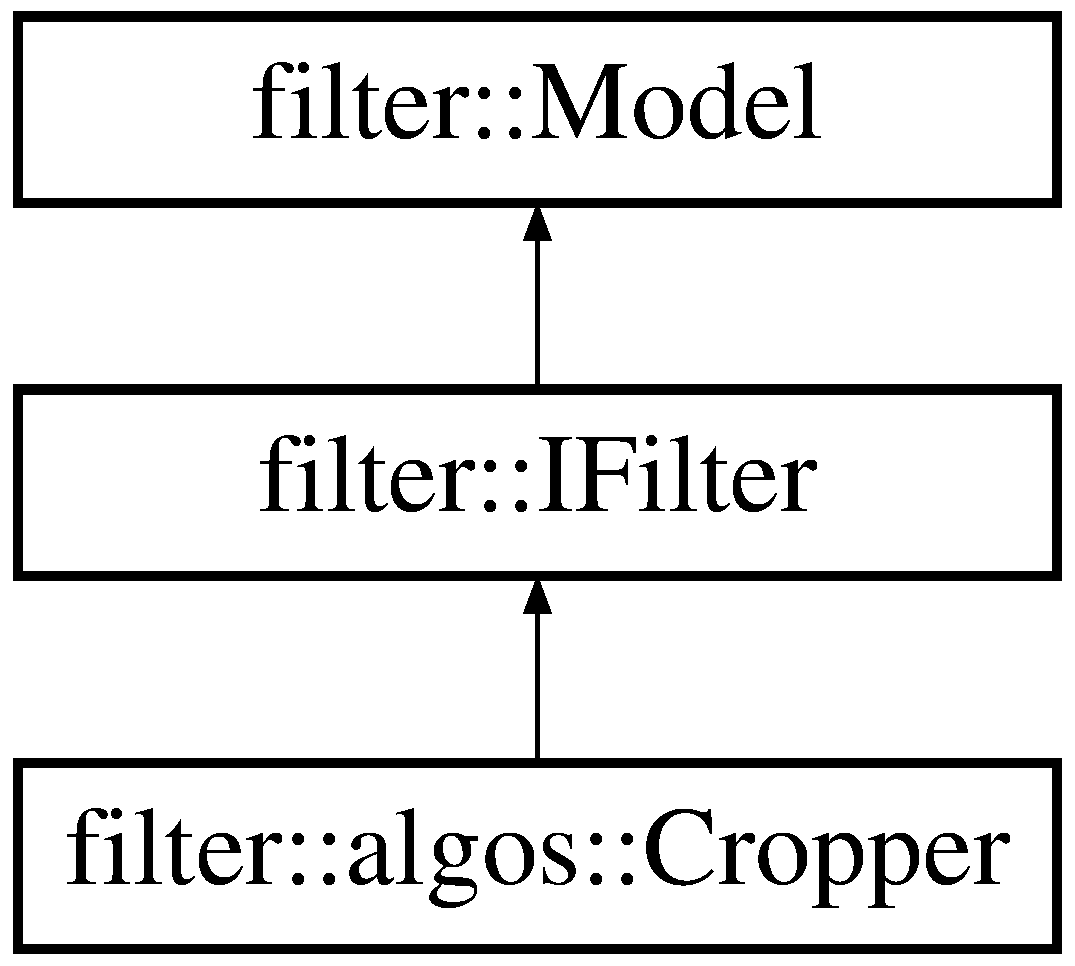
\includegraphics[height=3.000000cm]{d5/d9d/classfilter_1_1algos_1_1_cropper}
\end{center}
\end{figure}
\subsection*{Classes}
\begin{DoxyCompactItemize}
\item 
class \hyperlink{classfilter_1_1algos_1_1_cropper_1_1_c_v_cropper_data}{C\+V\+Cropper\+Data}
\begin{DoxyCompactList}\small\item\em The \hyperlink{classfilter_1_1algos_1_1_cropper_1_1_c_v_cropper_data}{C\+V\+Cropper\+Data} class stores the data relative to where the user clicked on an Open\+CV window. \end{DoxyCompactList}\end{DoxyCompactItemize}
\subsection*{Public Types}
\begin{DoxyCompactItemize}
\item 
\mbox{\Hypertarget{classfilter_1_1algos_1_1_cropper_a11c140066a6f2ab920f681dfbf805d72}\label{classfilter_1_1algos_1_1_cropper_a11c140066a6f2ab920f681dfbf805d72}} 
typedef \hyperlink{class_proxy_functor}{Proxy\+Functor}$<$ \hyperlink{classfilter_1_1algos_1_1_cropper}{Cropper} $>$ {\bfseries \+\_\+proxy\+Functor}
\item 
\mbox{\Hypertarget{classfilter_1_1algos_1_1_cropper_aef731a216e801db61284b47f33d19033}\label{classfilter_1_1algos_1_1_cropper_aef731a216e801db61284b47f33d19033}} 
typedef \hyperlink{classfilter_1_1algos_1_1_cropper}{Cropper} {\bfseries mytype}
\item 
\mbox{\Hypertarget{classfilter_1_1algos_1_1_cropper_aa90d073a66e20ca9164736d0449cc2c1}\label{classfilter_1_1algos_1_1_cropper_aa90d073a66e20ca9164736d0449cc2c1}} 
typedef bool {\bfseries vartype\+\_\+\+\_\+wait}
\end{DoxyCompactItemize}
\subsection*{Public Member Functions}
\begin{DoxyCompactItemize}
\item 
\mbox{\Hypertarget{classfilter_1_1algos_1_1_cropper_aaf461702ce09f1f72ac270f4724ebf2f}\label{classfilter_1_1algos_1_1_cropper_aaf461702ce09f1f72ac270f4724ebf2f}} 
virtual \hyperlink{classfilter_1_1data_1_1_connex_data_base}{data\+::\+Connex\+Data\+Base} \& {\bfseries get\+Connector} ()
\item 
\mbox{\Hypertarget{classfilter_1_1algos_1_1_cropper_a8654c44540b0823032b0a78a8ab537fa}\label{classfilter_1_1algos_1_1_cropper_a8654c44540b0823032b0a78a8ab537fa}} 
void {\bfseries set\+\_\+wait\+\_\+from\+\_\+json} (boost\+::property\+\_\+tree\+::ptree \&json\+Class)
\item 
\mbox{\Hypertarget{classfilter_1_1algos_1_1_cropper_a385b712ebd79b5c12fcd14d3b08f6454}\label{classfilter_1_1algos_1_1_cropper_a385b712ebd79b5c12fcd14d3b08f6454}} 
void {\bfseries set\+\_\+wait} (vartype\+\_\+\+\_\+wait \&\+\_\+\+\_\+wait)
\item 
\mbox{\Hypertarget{classfilter_1_1algos_1_1_cropper_a8374338b813a8372844a66ba01531aa1}\label{classfilter_1_1algos_1_1_cropper_a8374338b813a8372844a66ba01531aa1}} 
vartype\+\_\+\+\_\+wait {\bfseries get\+\_\+wait} ()
\item 
\mbox{\Hypertarget{classfilter_1_1algos_1_1_cropper_af125f693a714d3cf00b53b7560c3fbad}\label{classfilter_1_1algos_1_1_cropper_af125f693a714d3cf00b53b7560c3fbad}} 
void {\bfseries copy\+\_\+wait} (\hyperlink{classfilter_1_1algos_1_1_cropper}{mytype} $\ast$instance)
\item 
virtual std\+::string \hyperlink{classfilter_1_1algos_1_1_cropper_ae970d5d448587b8288aca2484f12f2fa}{result\+As\+String} ()
\begin{DoxyCompactList}\small\item\em Get the result of the processing done by the node. This method will return information only. The actual processing is done by the process() method. \end{DoxyCompactList}\item 
\mbox{\Hypertarget{classfilter_1_1algos_1_1_cropper_a34450cda9e5468d6f37f0c5281fe225e}\label{classfilter_1_1algos_1_1_cropper_a34450cda9e5468d6f37f0c5281fe225e}} 
Hipe\+Status {\bfseries process} ()
\item 
\mbox{\Hypertarget{classfilter_1_1algos_1_1_cropper_af8c56025560a142af00defbb74d228d6}\label{classfilter_1_1algos_1_1_cropper_af8c56025560a142af00defbb74d228d6}} 
void {\bfseries dispose} ()
\end{DoxyCompactItemize}
\subsection*{Public Attributes}
\begin{DoxyCompactItemize}
\item 
\mbox{\Hypertarget{classfilter_1_1algos_1_1_cropper_a73cbec21aefec48331f61324706e757d}\label{classfilter_1_1algos_1_1_cropper_a73cbec21aefec48331f61324706e757d}} 
std\+::shared\+\_\+ptr$<$ \hyperlink{classfilter_1_1data_1_1_pattern_data}{data\+::\+Pattern\+Data} $>$ {\bfseries \+\_\+pattern}
\item 
\mbox{\Hypertarget{classfilter_1_1algos_1_1_cropper_aa26d4d1e7a0f01e81f8bd3e55deffd8d}\label{classfilter_1_1algos_1_1_cropper_aa26d4d1e7a0f01e81f8bd3e55deffd8d}} 
std\+::shared\+\_\+ptr$<$ boost\+::thread $>$ {\bfseries \+\_\+task}
\item 
\mbox{\Hypertarget{classfilter_1_1algos_1_1_cropper_a73991942b18729185075c88cb1bd9ad4}\label{classfilter_1_1algos_1_1_cropper_a73991942b18729185075c88cb1bd9ad4}} 
std\+::shared\+\_\+ptr$<$ \hyperlink{classfilter_1_1algos_1_1_cropper_1_1_c_v_cropper_data}{C\+V\+Cropper\+Data} $>$ {\bfseries \+\_\+cv\+Cropper\+Data}
\item 
\mbox{\Hypertarget{classfilter_1_1algos_1_1_cropper_a9e4dab0a308ad6fee25d6d471c8dc908}\label{classfilter_1_1algos_1_1_cropper_a9e4dab0a308ad6fee25d6d471c8dc908}} 
\hyperlink{classfilter_1_1data_1_1_connex_data}{data\+::\+Connex\+Data}$<$ \hyperlink{classfilter_1_1data_1_1_image_data}{data\+::\+Image\+Data}, \hyperlink{classfilter_1_1data_1_1_pattern_data}{data\+::\+Pattern\+Data} $>$ {\bfseries \+\_\+connex\+Data}
\item 
bool \hyperlink{classfilter_1_1algos_1_1_cropper_ac7cf2a54e81d9227dc22b46d54603c7e}{wait}
\begin{DoxyCompactList}\small\item\em The \hyperlink{classfilter_1_1algos_1_1_cropper}{Cropper} filter will let the user select regions of interest in an image. \end{DoxyCompactList}\end{DoxyCompactItemize}
\subsection*{Private Member Functions}
\begin{DoxyCompactItemize}
\item 
void \hyperlink{classfilter_1_1algos_1_1_cropper_ad3cd43717d82f4d581bc2a1ed5f545e6}{window\+Task} (std\+::shared\+\_\+ptr$<$ \hyperlink{classfilter_1_1algos_1_1_cropper_1_1_c_v_cropper_data}{filter\+::algos\+::\+Cropper\+::\+C\+V\+Cropper\+Data} $>$ cv\+Cropper\+Data)
\begin{DoxyCompactList}\small\item\em Wrapper method to let the user select areas in an image. \end{DoxyCompactList}\item 
\mbox{\Hypertarget{classfilter_1_1algos_1_1_cropper_a80cfdd159bee1bbfd071797e5d176193}\label{classfilter_1_1algos_1_1_cropper_a80cfdd159bee1bbfd071797e5d176193}} 
void {\bfseries Cropper\+Area\+Drawer} ()
\end{DoxyCompactItemize}
\subsection*{Additional Inherited Members}


\subsection{Member Function Documentation}
\mbox{\Hypertarget{classfilter_1_1algos_1_1_cropper_ae970d5d448587b8288aca2484f12f2fa}\label{classfilter_1_1algos_1_1_cropper_ae970d5d448587b8288aca2484f12f2fa}} 
\index{filter\+::algos\+::\+Cropper@{filter\+::algos\+::\+Cropper}!result\+As\+String@{result\+As\+String}}
\index{result\+As\+String@{result\+As\+String}!filter\+::algos\+::\+Cropper@{filter\+::algos\+::\+Cropper}}
\subsubsection{\texorpdfstring{result\+As\+String()}{resultAsString()}}
{\footnotesize\ttfamily virtual std\+::string filter\+::algos\+::\+Cropper\+::result\+As\+String (\begin{DoxyParamCaption}{ }\end{DoxyParamCaption})\hspace{0.3cm}{\ttfamily [inline]}, {\ttfamily [virtual]}}

\begin{DoxyReturn}{Returns}
A string containing the result of the processing done by the filter. 
\end{DoxyReturn}


Reimplemented from \hyperlink{classfilter_1_1_i_filter_ab99902b060a6d9edc3452a8c9f85e37e}{filter\+::\+I\+Filter}.

\mbox{\Hypertarget{classfilter_1_1algos_1_1_cropper_ad3cd43717d82f4d581bc2a1ed5f545e6}\label{classfilter_1_1algos_1_1_cropper_ad3cd43717d82f4d581bc2a1ed5f545e6}} 
\index{filter\+::algos\+::\+Cropper@{filter\+::algos\+::\+Cropper}!window\+Task@{window\+Task}}
\index{window\+Task@{window\+Task}!filter\+::algos\+::\+Cropper@{filter\+::algos\+::\+Cropper}}
\subsubsection{\texorpdfstring{window\+Task()}{windowTask()}}
{\footnotesize\ttfamily void filter\+::algos\+::\+Cropper\+::window\+Task (\begin{DoxyParamCaption}\item[{std\+::shared\+\_\+ptr$<$ \hyperlink{classfilter_1_1algos_1_1_cropper_1_1_c_v_cropper_data}{filter\+::algos\+::\+Cropper\+::\+C\+V\+Cropper\+Data} $>$}]{cv\+Cropper\+Data }\end{DoxyParamCaption})\hspace{0.3cm}{\ttfamily [inline]}, {\ttfamily [private]}}


\begin{DoxyParams}{Parameters}
{\em cv\+Cropper\+Data} & The \hyperlink{classfilter_1_1algos_1_1_cropper_1_1_c_v_cropper_data}{C\+V\+Cropper\+Data} object to populate from user input. \\
\hline
\end{DoxyParams}


\subsection{Member Data Documentation}
\mbox{\Hypertarget{classfilter_1_1algos_1_1_cropper_ac7cf2a54e81d9227dc22b46d54603c7e}\label{classfilter_1_1algos_1_1_cropper_ac7cf2a54e81d9227dc22b46d54603c7e}} 
\index{filter\+::algos\+::\+Cropper@{filter\+::algos\+::\+Cropper}!wait@{wait}}
\index{wait@{wait}!filter\+::algos\+::\+Cropper@{filter\+::algos\+::\+Cropper}}
\subsubsection{\texorpdfstring{wait}{wait}}
{\footnotesize\ttfamily filter\+::algos\+::\+Cropper\+::wait}

\begin{DoxyRefDesc}{Todo}
\item[\hyperlink{todo__todo000006}{Todo}]\end{DoxyRefDesc}
The filter will extract the relative data of the selected regions of interest and return them as a Pattern\+Data object. The \hyperlink{classfilter_1_1algos_1_1_cropper}{Cropper} filter runs in a separate thread.

\mbox{[}T\+O\+DO\mbox{]} 

The documentation for this class was generated from the following file\+:\begin{DoxyCompactItemize}
\item 
header/filter/\+Algos/Cropper.\+h\end{DoxyCompactItemize}

\hypertarget{class_simple_web_1_1_crypto}{}\section{Simple\+Web\+:\+:Crypto Class Reference}
\label{class_simple_web_1_1_crypto}\index{Simple\+Web\+::\+Crypto@{Simple\+Web\+::\+Crypto}}
\subsection*{Classes}
\begin{DoxyCompactItemize}
\item 
class \hyperlink{class_simple_web_1_1_crypto_1_1_base64}{Base64}
\end{DoxyCompactItemize}
\subsection*{Static Public Member Functions}
\begin{DoxyCompactItemize}
\item 
\mbox{\Hypertarget{class_simple_web_1_1_crypto_ab40abff25234f08b7b90fc97fab39faa}\label{class_simple_web_1_1_crypto_ab40abff25234f08b7b90fc97fab39faa}} 
static std\+::string \hyperlink{class_simple_web_1_1_crypto_ab40abff25234f08b7b90fc97fab39faa}{to\+\_\+hex\+\_\+string} (const std\+::string \&input)
\begin{DoxyCompactList}\small\item\em Return hex string from bytes in input string. \end{DoxyCompactList}\item 
\mbox{\Hypertarget{class_simple_web_1_1_crypto_a0561dc11ae3cd68004bdb90e04252164}\label{class_simple_web_1_1_crypto_a0561dc11ae3cd68004bdb90e04252164}} 
static std\+::string {\bfseries md5} (const std\+::string \&input, size\+\_\+t iterations=1)
\item 
\mbox{\Hypertarget{class_simple_web_1_1_crypto_a8fe52ed7463c99a9165a215831dc6127}\label{class_simple_web_1_1_crypto_a8fe52ed7463c99a9165a215831dc6127}} 
static std\+::string {\bfseries md5} (std\+::istream \&stream, size\+\_\+t iterations=1)
\item 
\mbox{\Hypertarget{class_simple_web_1_1_crypto_a7c665ab1dc299e741a5e81f7cf33c523}\label{class_simple_web_1_1_crypto_a7c665ab1dc299e741a5e81f7cf33c523}} 
static std\+::string {\bfseries sha1} (const std\+::string \&input, size\+\_\+t iterations=1)
\item 
\mbox{\Hypertarget{class_simple_web_1_1_crypto_a638b7c19084f34d88d696be9d9353e4e}\label{class_simple_web_1_1_crypto_a638b7c19084f34d88d696be9d9353e4e}} 
static std\+::string {\bfseries sha1} (std\+::istream \&stream, size\+\_\+t iterations=1)
\item 
\mbox{\Hypertarget{class_simple_web_1_1_crypto_a85dc4f2bae2305fa6e8a34bf0f4f158d}\label{class_simple_web_1_1_crypto_a85dc4f2bae2305fa6e8a34bf0f4f158d}} 
static std\+::string {\bfseries sha256} (const std\+::string \&input, size\+\_\+t iterations=1)
\item 
\mbox{\Hypertarget{class_simple_web_1_1_crypto_a09d10275fef3ec75a698af4f27c5aac3}\label{class_simple_web_1_1_crypto_a09d10275fef3ec75a698af4f27c5aac3}} 
static std\+::string {\bfseries sha256} (std\+::istream \&stream, size\+\_\+t iterations=1)
\item 
\mbox{\Hypertarget{class_simple_web_1_1_crypto_adc77ea749230d6a7f299125c43966c34}\label{class_simple_web_1_1_crypto_adc77ea749230d6a7f299125c43966c34}} 
static std\+::string {\bfseries sha512} (const std\+::string \&input, size\+\_\+t iterations=1)
\item 
\mbox{\Hypertarget{class_simple_web_1_1_crypto_a95b77524631a18e1fd1e2584e062d452}\label{class_simple_web_1_1_crypto_a95b77524631a18e1fd1e2584e062d452}} 
static std\+::string {\bfseries sha512} (std\+::istream \&stream, size\+\_\+t iterations=1)
\item 
\mbox{\Hypertarget{class_simple_web_1_1_crypto_a53d0a191ebda80d31c291260343e38fe}\label{class_simple_web_1_1_crypto_a53d0a191ebda80d31c291260343e38fe}} 
static std\+::string \hyperlink{class_simple_web_1_1_crypto_a53d0a191ebda80d31c291260343e38fe}{pbkdf2} (const std\+::string \&password, const std\+::string \&salt, int iterations, int key\+\_\+size)
\begin{DoxyCompactList}\small\item\em key\+\_\+size is number of bytes of the returned key. \end{DoxyCompactList}\end{DoxyCompactItemize}
\subsection*{Static Private Attributes}
\begin{DoxyCompactItemize}
\item 
\mbox{\Hypertarget{class_simple_web_1_1_crypto_a535775900225f463e7ed14f984695865}\label{class_simple_web_1_1_crypto_a535775900225f463e7ed14f984695865}} 
static const size\+\_\+t {\bfseries buffer\+\_\+size} =131072
\end{DoxyCompactItemize}


The documentation for this class was generated from the following file\+:\begin{DoxyCompactItemize}
\item 
header/http/crypto.\+hpp\end{DoxyCompactItemize}

\hypertarget{classfilter_1_1algos_1_1_cropper_1_1_c_v_cropper_data}{}\section{filter\+:\+:algos\+:\+:Cropper\+:\+:C\+V\+Cropper\+Data Class Reference}
\label{classfilter_1_1algos_1_1_cropper_1_1_c_v_cropper_data}\index{filter\+::algos\+::\+Cropper\+::\+C\+V\+Cropper\+Data@{filter\+::algos\+::\+Cropper\+::\+C\+V\+Cropper\+Data}}


The \hyperlink{classfilter_1_1algos_1_1_cropper_1_1_c_v_cropper_data}{C\+V\+Cropper\+Data} class stores the data relative to where the user clicked on an Open\+CV window.  




{\ttfamily \#include $<$Cropper.\+h$>$}

\subsection*{Public Member Functions}
\begin{DoxyCompactItemize}
\item 
\hyperlink{classfilter_1_1algos_1_1_cropper_1_1_c_v_cropper_data_a8f2195d489fd541b9add781355bc99c2}{C\+V\+Cropper\+Data} (const \hyperlink{classfilter_1_1data_1_1_pattern_data}{data\+::\+Pattern\+Data} \&pat)
\begin{DoxyCompactList}\small\item\em \hyperlink{classfilter_1_1algos_1_1_cropper_1_1_c_v_cropper_data}{C\+V\+Cropper\+Data} constructor with Pattern\+Data parameter. Will add data to it. \end{DoxyCompactList}\item 
\hyperlink{classfilter_1_1algos_1_1_cropper_1_1_c_v_cropper_data_ad0dc18f5cb03ab6abcaa4dfea9594ae6}{C\+V\+Cropper\+Data} (\hyperlink{classfilter_1_1data_1_1_image_data}{data\+::\+Image\+Data} \&image)
\begin{DoxyCompactList}\small\item\em \hyperlink{classfilter_1_1algos_1_1_cropper_1_1_c_v_cropper_data}{C\+V\+Cropper\+Data} constructor with image parameter. \mbox{[}T\+O\+DO\mbox{]}. \end{DoxyCompactList}\item 
\mbox{\Hypertarget{classfilter_1_1algos_1_1_cropper_1_1_c_v_cropper_data_a0ab57924d1fb875cd180416d7616e33e}\label{classfilter_1_1algos_1_1_cropper_1_1_c_v_cropper_data_a0ab57924d1fb875cd180416d7616e33e}} 
\hyperlink{classfilter_1_1algos_1_1_cropper_1_1_c_v_cropper_data_a0ab57924d1fb875cd180416d7616e33e}{C\+V\+Cropper\+Data} ()
\begin{DoxyCompactList}\small\item\em \hyperlink{classfilter_1_1algos_1_1_cropper_1_1_c_v_cropper_data}{C\+V\+Cropper\+Data} default constructor. \mbox{[}T\+O\+DO\mbox{]}. \end{DoxyCompactList}\item 
\hyperlink{classfilter_1_1algos_1_1_cropper_1_1_c_v_cropper_data}{C\+V\+Cropper\+Data} \& \hyperlink{classfilter_1_1algos_1_1_cropper_1_1_c_v_cropper_data_a8f551ce95e4cea54230ddbbd5b1cc6db}{operator$<$$<$} (\hyperlink{classfilter_1_1data_1_1_image_data}{data\+::\+Image\+Data} \&input\+Image)
\begin{DoxyCompactList}\small\item\em Overloaded insertion operator used to overwrite the \hyperlink{classfilter_1_1algos_1_1_cropper_1_1_c_v_cropper_data}{C\+V\+Cropper\+Data}\textquotesingle{}s Pattern\+Data field\textquotesingle{}s request image. \end{DoxyCompactList}\item 
\hyperlink{classfilter_1_1algos_1_1_cropper_1_1_c_v_cropper_data}{C\+V\+Cropper\+Data} \& \hyperlink{classfilter_1_1algos_1_1_cropper_1_1_c_v_cropper_data_a74dba06cb470f371cd3658f6a11021e6}{operator$<$$<$} (cv\+::\+Mat input\+Image)
\begin{DoxyCompactList}\small\item\em Overloaded insertion operator used to overwrite the \hyperlink{classfilter_1_1algos_1_1_cropper_1_1_c_v_cropper_data}{C\+V\+Cropper\+Data}\textquotesingle{}s Pattern\+Data afield\textquotesingle{}s request image. \end{DoxyCompactList}\end{DoxyCompactItemize}
\subsection*{Public Attributes}
\begin{DoxyCompactItemize}
\item 
\mbox{\Hypertarget{classfilter_1_1algos_1_1_cropper_1_1_c_v_cropper_data_a125d07318b2bcfecc55ac734d90b40f4}\label{classfilter_1_1algos_1_1_cropper_1_1_c_v_cropper_data_a125d07318b2bcfecc55ac734d90b40f4}} 
std\+::atomic$<$ bool $>$ {\bfseries clicked}
\item 
\mbox{\Hypertarget{classfilter_1_1algos_1_1_cropper_1_1_c_v_cropper_data_aa3d335abd590fb5f988015e6702b0cb6}\label{classfilter_1_1algos_1_1_cropper_1_1_c_v_cropper_data_aa3d335abd590fb5f988015e6702b0cb6}} 
std\+::atomic$<$ bool $>$ {\bfseries drawing}
\item 
\mbox{\Hypertarget{classfilter_1_1algos_1_1_cropper_1_1_c_v_cropper_data_a5287f1b333d8f677e1fd50634ec4837a}\label{classfilter_1_1algos_1_1_cropper_1_1_c_v_cropper_data_a5287f1b333d8f677e1fd50634ec4837a}} 
int {\bfseries index}
\item 
\mbox{\Hypertarget{classfilter_1_1algos_1_1_cropper_1_1_c_v_cropper_data_a7e35a7d215081ccab6e81ef6d3b136ab}\label{classfilter_1_1algos_1_1_cropper_1_1_c_v_cropper_data_a7e35a7d215081ccab6e81ef6d3b136ab}} 
cv\+::\+String {\bfseries window\+Name}
\item 
\mbox{\Hypertarget{classfilter_1_1algos_1_1_cropper_1_1_c_v_cropper_data_a9781d33a959e2c47ccd407a8ee4727a3}\label{classfilter_1_1algos_1_1_cropper_1_1_c_v_cropper_data_a9781d33a959e2c47ccd407a8ee4727a3}} 
std\+::vector$<$ cv\+::\+Point $>$ {\bfseries rectangle}
\item 
\mbox{\Hypertarget{classfilter_1_1algos_1_1_cropper_1_1_c_v_cropper_data_aecc2f83db50367e3cebda74e5e80d702}\label{classfilter_1_1algos_1_1_cropper_1_1_c_v_cropper_data_aecc2f83db50367e3cebda74e5e80d702}} 
cv\+::\+Mat {\bfseries sand\+Box\+Image}
\item 
\mbox{\Hypertarget{classfilter_1_1algos_1_1_cropper_1_1_c_v_cropper_data_a699cc8f85489274de5170d2d0e4fe10c}\label{classfilter_1_1algos_1_1_cropper_1_1_c_v_cropper_data_a699cc8f85489274de5170d2d0e4fe10c}} 
cv\+::\+Mat {\bfseries sand\+Box\+Image\+\_\+backup}
\item 
\mbox{\Hypertarget{classfilter_1_1algos_1_1_cropper_1_1_c_v_cropper_data_a678ee25c91960fa20892a2c2d7346cf0}\label{classfilter_1_1algos_1_1_cropper_1_1_c_v_cropper_data_a678ee25c91960fa20892a2c2d7346cf0}} 
\hyperlink{classfilter_1_1data_1_1_pattern_data}{data\+::\+Pattern\+Data} {\bfseries pattern}
\item 
\mbox{\Hypertarget{classfilter_1_1algos_1_1_cropper_1_1_c_v_cropper_data_a63b558ac47f3f8864f11a747c5736a51}\label{classfilter_1_1algos_1_1_cropper_1_1_c_v_cropper_data_a63b558ac47f3f8864f11a747c5736a51}} 
std\+::atomic$<$ bool $>$ {\bfseries started}
\item 
\mbox{\Hypertarget{classfilter_1_1algos_1_1_cropper_1_1_c_v_cropper_data_a0504eb12cf887367e48a509e976b4b88}\label{classfilter_1_1algos_1_1_cropper_1_1_c_v_cropper_data_a0504eb12cf887367e48a509e976b4b88}} 
\hyperlink{classcore_1_1queue_1_1_concurrent_queue}{core\+::queue\+::\+Concurrent\+Queue}$<$ std\+::vector$<$ cv\+::\+Point $>$ $>$ {\bfseries array\+Crop}
\end{DoxyCompactItemize}


\subsection{Constructor \& Destructor Documentation}
\mbox{\Hypertarget{classfilter_1_1algos_1_1_cropper_1_1_c_v_cropper_data_a8f2195d489fd541b9add781355bc99c2}\label{classfilter_1_1algos_1_1_cropper_1_1_c_v_cropper_data_a8f2195d489fd541b9add781355bc99c2}} 
\index{filter\+::algos\+::\+Cropper\+::\+C\+V\+Cropper\+Data@{filter\+::algos\+::\+Cropper\+::\+C\+V\+Cropper\+Data}!C\+V\+Cropper\+Data@{C\+V\+Cropper\+Data}}
\index{C\+V\+Cropper\+Data@{C\+V\+Cropper\+Data}!filter\+::algos\+::\+Cropper\+::\+C\+V\+Cropper\+Data@{filter\+::algos\+::\+Cropper\+::\+C\+V\+Cropper\+Data}}
\subsubsection{\texorpdfstring{C\+V\+Cropper\+Data()}{CVCropperData()}\hspace{0.1cm}{\footnotesize\ttfamily [1/2]}}
{\footnotesize\ttfamily filter\+::algos\+::\+Cropper\+::\+C\+V\+Cropper\+Data\+::\+C\+V\+Cropper\+Data (\begin{DoxyParamCaption}\item[{const \hyperlink{classfilter_1_1data_1_1_pattern_data}{data\+::\+Pattern\+Data} \&}]{pat }\end{DoxyParamCaption})\hspace{0.3cm}{\ttfamily [inline]}}

\begin{DoxyRefDesc}{Todo}
\item[\hyperlink{todo__todo000007}{Todo}]\end{DoxyRefDesc}

\begin{DoxyParams}{Parameters}
{\em pat} & Pattern\+Data object to start from. \\
\hline
\end{DoxyParams}
\mbox{\Hypertarget{classfilter_1_1algos_1_1_cropper_1_1_c_v_cropper_data_ad0dc18f5cb03ab6abcaa4dfea9594ae6}\label{classfilter_1_1algos_1_1_cropper_1_1_c_v_cropper_data_ad0dc18f5cb03ab6abcaa4dfea9594ae6}} 
\index{filter\+::algos\+::\+Cropper\+::\+C\+V\+Cropper\+Data@{filter\+::algos\+::\+Cropper\+::\+C\+V\+Cropper\+Data}!C\+V\+Cropper\+Data@{C\+V\+Cropper\+Data}}
\index{C\+V\+Cropper\+Data@{C\+V\+Cropper\+Data}!filter\+::algos\+::\+Cropper\+::\+C\+V\+Cropper\+Data@{filter\+::algos\+::\+Cropper\+::\+C\+V\+Cropper\+Data}}
\subsubsection{\texorpdfstring{C\+V\+Cropper\+Data()}{CVCropperData()}\hspace{0.1cm}{\footnotesize\ttfamily [2/2]}}
{\footnotesize\ttfamily filter\+::algos\+::\+Cropper\+::\+C\+V\+Cropper\+Data\+::\+C\+V\+Cropper\+Data (\begin{DoxyParamCaption}\item[{\hyperlink{classfilter_1_1data_1_1_image_data}{data\+::\+Image\+Data} \&}]{image }\end{DoxyParamCaption})\hspace{0.3cm}{\ttfamily [inline]}}


\begin{DoxyParams}{Parameters}
{\em image} & \mbox{[}T\+O\+DO\mbox{]} \\
\hline
\end{DoxyParams}


\subsection{Member Function Documentation}
\mbox{\Hypertarget{classfilter_1_1algos_1_1_cropper_1_1_c_v_cropper_data_a8f551ce95e4cea54230ddbbd5b1cc6db}\label{classfilter_1_1algos_1_1_cropper_1_1_c_v_cropper_data_a8f551ce95e4cea54230ddbbd5b1cc6db}} 
\index{filter\+::algos\+::\+Cropper\+::\+C\+V\+Cropper\+Data@{filter\+::algos\+::\+Cropper\+::\+C\+V\+Cropper\+Data}!operator$<$$<$@{operator$<$$<$}}
\index{operator$<$$<$@{operator$<$$<$}!filter\+::algos\+::\+Cropper\+::\+C\+V\+Cropper\+Data@{filter\+::algos\+::\+Cropper\+::\+C\+V\+Cropper\+Data}}
\subsubsection{\texorpdfstring{operator$<$$<$()}{operator<<()}\hspace{0.1cm}{\footnotesize\ttfamily [1/2]}}
{\footnotesize\ttfamily \hyperlink{classfilter_1_1algos_1_1_cropper_1_1_c_v_cropper_data}{C\+V\+Cropper\+Data}\& filter\+::algos\+::\+Cropper\+::\+C\+V\+Cropper\+Data\+::operator$<$$<$ (\begin{DoxyParamCaption}\item[{\hyperlink{classfilter_1_1data_1_1_image_data}{data\+::\+Image\+Data} \&}]{input\+Image }\end{DoxyParamCaption})\hspace{0.3cm}{\ttfamily [inline]}}


\begin{DoxyParams}{Parameters}
{\em input\+Image} & The image which will be used to overwrite the Pattern\+Data request image. \\
\hline
\end{DoxyParams}
\begin{DoxyReturn}{Returns}
Returns a reference to the \hyperlink{classfilter_1_1algos_1_1_cropper_1_1_c_v_cropper_data}{C\+V\+Cropper\+Data} object. 
\end{DoxyReturn}
\mbox{\Hypertarget{classfilter_1_1algos_1_1_cropper_1_1_c_v_cropper_data_a74dba06cb470f371cd3658f6a11021e6}\label{classfilter_1_1algos_1_1_cropper_1_1_c_v_cropper_data_a74dba06cb470f371cd3658f6a11021e6}} 
\index{filter\+::algos\+::\+Cropper\+::\+C\+V\+Cropper\+Data@{filter\+::algos\+::\+Cropper\+::\+C\+V\+Cropper\+Data}!operator$<$$<$@{operator$<$$<$}}
\index{operator$<$$<$@{operator$<$$<$}!filter\+::algos\+::\+Cropper\+::\+C\+V\+Cropper\+Data@{filter\+::algos\+::\+Cropper\+::\+C\+V\+Cropper\+Data}}
\subsubsection{\texorpdfstring{operator$<$$<$()}{operator<<()}\hspace{0.1cm}{\footnotesize\ttfamily [2/2]}}
{\footnotesize\ttfamily \hyperlink{classfilter_1_1algos_1_1_cropper_1_1_c_v_cropper_data}{C\+V\+Cropper\+Data}\& filter\+::algos\+::\+Cropper\+::\+C\+V\+Cropper\+Data\+::operator$<$$<$ (\begin{DoxyParamCaption}\item[{cv\+::\+Mat}]{input\+Image }\end{DoxyParamCaption})\hspace{0.3cm}{\ttfamily [inline]}}


\begin{DoxyParams}{Parameters}
{\em input\+Image} & The image which will be used to overwrite the Pattern\+Data request image. \\
\hline
\end{DoxyParams}
\begin{DoxyReturn}{Returns}
Returns a reference to the \hyperlink{classfilter_1_1algos_1_1_cropper_1_1_c_v_cropper_data}{C\+V\+Cropper\+Data} object. 
\end{DoxyReturn}


The documentation for this class was generated from the following file\+:\begin{DoxyCompactItemize}
\item 
header/filter/\+Algos/Cropper.\+h\end{DoxyCompactItemize}

\hypertarget{classfilter_1_1data_1_1_data}{}\section{filter\+:\+:data\+:\+:Data Class Reference}
\label{classfilter_1_1data_1_1_data}\index{filter\+::data\+::\+Data@{filter\+::data\+::\+Data}}
Inheritance diagram for filter\+:\+:data\+:\+:Data\+:\begin{figure}[H]
\begin{center}
\leavevmode
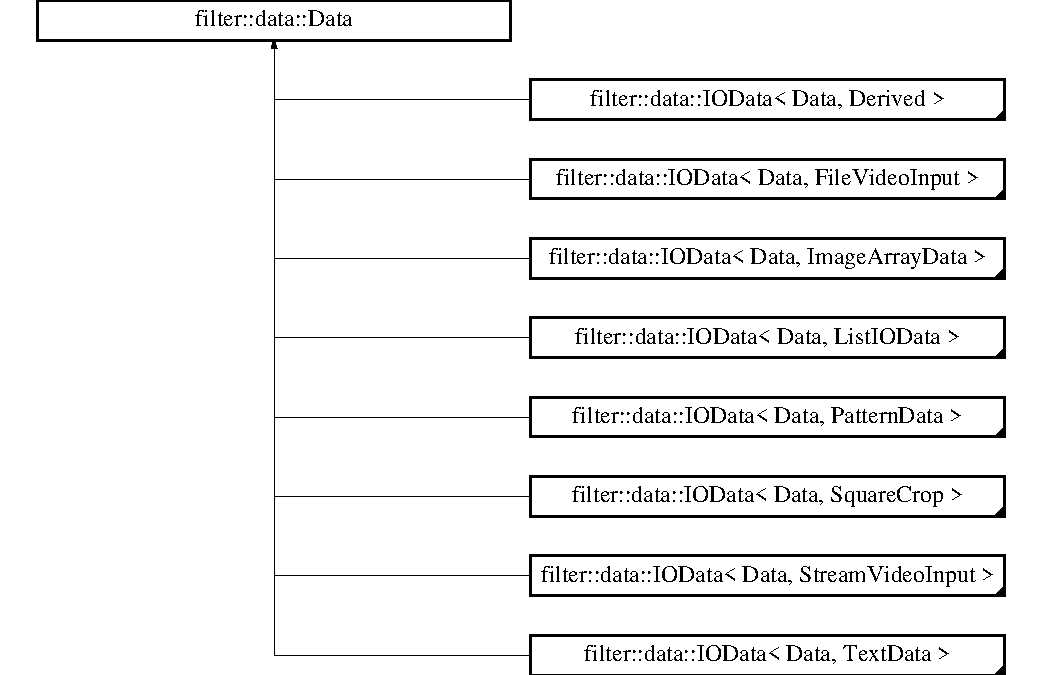
\includegraphics[height=9.000000cm]{d4/d8e/classfilter_1_1data_1_1_data}
\end{center}
\end{figure}
\subsection*{Public Types}
\begin{DoxyCompactItemize}
\item 
\mbox{\Hypertarget{classfilter_1_1data_1_1_data_ad9c9ffde07366691a9e9a1de3147a8a7}\label{classfilter_1_1data_1_1_data_ad9c9ffde07366691a9e9a1de3147a8a7}} 
typedef \hyperlink{classfilter_1_1data_1_1_data}{Data} {\bfseries \+\_\+classtype}
\end{DoxyCompactItemize}
\subsection*{Public Member Functions}
\begin{DoxyCompactItemize}
\item 
\mbox{\Hypertarget{classfilter_1_1data_1_1_data_acc0dcf88474d97ff83aaa720206823d2}\label{classfilter_1_1data_1_1_data_acc0dcf88474d97ff83aaa720206823d2}} 
{\bfseries Data} (const \hyperlink{classfilter_1_1data_1_1_data}{Data} \&data)
\item 
\mbox{\Hypertarget{classfilter_1_1data_1_1_data_a53fe854b2f08c1dbb36c89507534b686}\label{classfilter_1_1data_1_1_data_a53fe854b2f08c1dbb36c89507534b686}} 
void {\bfseries register\+Instance} (const \hyperlink{classfilter_1_1data_1_1_data}{Data} \&child\+Instance)
\item 
\mbox{\Hypertarget{classfilter_1_1data_1_1_data_a5c520edda1a677fce2b17efea3e89f76}\label{classfilter_1_1data_1_1_data_a5c520edda1a677fce2b17efea3e89f76}} 
void {\bfseries register\+Instance} (\hyperlink{classfilter_1_1data_1_1_data}{Data} $\ast$child\+Instance)
\item 
\mbox{\Hypertarget{classfilter_1_1data_1_1_data_a64243539d0f374448a2e1fd211e534f0}\label{classfilter_1_1data_1_1_data_a64243539d0f374448a2e1fd211e534f0}} 
void {\bfseries register\+Instance} (std\+::shared\+\_\+ptr$<$ \hyperlink{classfilter_1_1data_1_1_data}{Data} $>$ child\+Instance)
\item 
\mbox{\Hypertarget{classfilter_1_1data_1_1_data_ae7cff6f7c57c4c3f495b3e268342870e}\label{classfilter_1_1data_1_1_data_ae7cff6f7c57c4c3f495b3e268342870e}} 
I\+O\+Data\+Type {\bfseries get\+Type} () const
\item 
\mbox{\Hypertarget{classfilter_1_1data_1_1_data_a6094f1de5517d63d5ed202cadc883acc}\label{classfilter_1_1data_1_1_data_a6094f1de5517d63d5ed202cadc883acc}} 
bool {\bfseries get\+Decorate} () const
\item 
\mbox{\Hypertarget{classfilter_1_1data_1_1_data_a7478bba941654186dd0bf8cd7cf639fc}\label{classfilter_1_1data_1_1_data_a7478bba941654186dd0bf8cd7cf639fc}} 
void {\bfseries copy\+Type\+To} (\hyperlink{classfilter_1_1data_1_1_data}{Data} \&left)
\item 
\mbox{\Hypertarget{classfilter_1_1data_1_1_data_aae174a103a5457c063dbcde8ad5b9338}\label{classfilter_1_1data_1_1_data_aae174a103a5457c063dbcde8ad5b9338}} 
virtual void {\bfseries copy\+To} (\hyperlink{classfilter_1_1data_1_1_data}{Data} \&left) const
\item 
\mbox{\Hypertarget{classfilter_1_1data_1_1_data_ac974955f3c516f66cbc2881e07ad5f15}\label{classfilter_1_1data_1_1_data_ac974955f3c516f66cbc2881e07ad5f15}} 
virtual bool {\bfseries empty} () const
\item 
\mbox{\Hypertarget{classfilter_1_1data_1_1_data_a3b51e933a2eefdda21d5e03fe9745c95}\label{classfilter_1_1data_1_1_data_a3b51e933a2eefdda21d5e03fe9745c95}} 
\hyperlink{classfilter_1_1data_1_1_data}{Data} \& {\bfseries operator=} (const \hyperlink{classfilter_1_1data_1_1_data}{Data} \&left)
\item 
\mbox{\Hypertarget{classfilter_1_1data_1_1_data_aaabb3dcd8311c387a445dff74e690909}\label{classfilter_1_1data_1_1_data_aaabb3dcd8311c387a445dff74e690909}} 
void {\bfseries release} ()
\end{DoxyCompactItemize}
\subsection*{Protected Member Functions}
\begin{DoxyCompactItemize}
\item 
\mbox{\Hypertarget{classfilter_1_1data_1_1_data_a1e19fabae8ee601353c40b799e2ce190}\label{classfilter_1_1data_1_1_data_a1e19fabae8ee601353c40b799e2ce190}} 
{\bfseries Data} (I\+O\+Data\+Type datatype)
\item 
\mbox{\Hypertarget{classfilter_1_1data_1_1_data_a770c9fef477e8cc75b71238a817aa0f9}\label{classfilter_1_1data_1_1_data_a770c9fef477e8cc75b71238a817aa0f9}} 
void {\bfseries set\+Type} (const I\+O\+Data\+Type io\+\_\+data\+\_\+type)
\end{DoxyCompactItemize}
\subsection*{Protected Attributes}
\begin{DoxyCompactItemize}
\item 
\mbox{\Hypertarget{classfilter_1_1data_1_1_data_aefb406c780862d52d3737baccc2637a8}\label{classfilter_1_1data_1_1_data_aefb406c780862d52d3737baccc2637a8}} 
I\+O\+Data\+Type {\bfseries \+\_\+type}
\item 
\mbox{\Hypertarget{classfilter_1_1data_1_1_data_a102327be7d0e7a08923a2d8a9a908407}\label{classfilter_1_1data_1_1_data_a102327be7d0e7a08923a2d8a9a908407}} 
std\+::shared\+\_\+ptr$<$ \hyperlink{classfilter_1_1data_1_1_data}{Data} $>$ {\bfseries \+\_\+\+This}
\item 
\mbox{\Hypertarget{classfilter_1_1data_1_1_data_af0923570708eec4f8c7e3c86c49a7ef9}\label{classfilter_1_1data_1_1_data_af0923570708eec4f8c7e3c86c49a7ef9}} 
bool {\bfseries \+\_\+decorate} = false
\end{DoxyCompactItemize}


The documentation for this class was generated from the following file\+:\begin{DoxyCompactItemize}
\item 
header/filter/data/I\+O\+Data.\+h\end{DoxyCompactItemize}

\hypertarget{class_data_access_mapper}{}\section{Data\+Access\+Mapper Class Reference}
\label{class_data_access_mapper}\index{Data\+Access\+Mapper@{Data\+Access\+Mapper}}
\subsection*{Static Public Member Functions}
\begin{DoxyCompactItemize}
\item 
\mbox{\Hypertarget{class_data_access_mapper_a4d16c181c23488bad84b5276ff2621c5}\label{class_data_access_mapper_a4d16c181c23488bad84b5276ff2621c5}} 
static Data\+Access {\bfseries get\+Access\+From\+String} (const std\+::string data\+Access\+String)
\end{DoxyCompactItemize}


The documentation for this class was generated from the following file\+:\begin{DoxyCompactItemize}
\item 
header/filter/data/Data\+Access.\+h\end{DoxyCompactItemize}

\hypertarget{classfilter_1_1data_1_1_data_port}{}\section{filter\+:\+:data\+:\+:Data\+Port Class Reference}
\label{classfilter_1_1data_1_1_data_port}\index{filter\+::data\+::\+Data\+Port@{filter\+::data\+::\+Data\+Port}}


\hyperlink{classfilter_1_1data_1_1_data}{Data} port contains the data to guarantee the transition with all Ifilter and I\+Model.  




{\ttfamily \#include $<$Connex\+Data.\+h$>$}

Inheritance diagram for filter\+:\+:data\+:\+:Data\+Port\+:\begin{figure}[H]
\begin{center}
\leavevmode
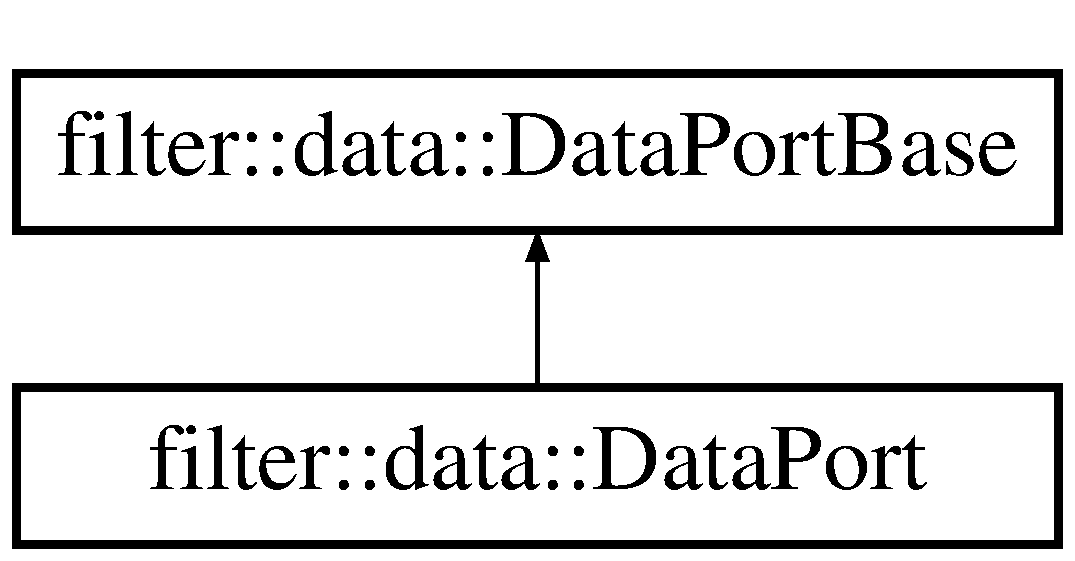
\includegraphics[height=2.000000cm]{d0/d37/classfilter_1_1data_1_1_data_port}
\end{center}
\end{figure}
\subsection*{Public Member Functions}
\begin{DoxyCompactItemize}
\item 
\hyperlink{classfilter_1_1data_1_1_data}{Data} \hyperlink{classfilter_1_1data_1_1_data_port_aab5c7164e7da8e31c92221ccbbcdfc82}{get} ()
\begin{DoxyCompactList}\small\item\em Alias to the \hyperlink{classfilter_1_1data_1_1_data_port_a236dbb70802799eb937cec5020b78bdd}{pop()} method. Get the port\textquotesingle{}s next stored data. \end{DoxyCompactList}\item 
\hyperlink{classfilter_1_1data_1_1_data}{Data} \hyperlink{classfilter_1_1data_1_1_data_port_a236dbb70802799eb937cec5020b78bdd}{pop} ()
\begin{DoxyCompactList}\small\item\em Get the port\textquotesingle{}s next stored data. \end{DoxyCompactList}\item 
void \hyperlink{classfilter_1_1data_1_1_data_port_ac3701e8da30bbc0d5f47a8dffc3dea23}{push} (\hyperlink{classfilter_1_1data_1_1_data}{Data} \&data\+In)
\begin{DoxyCompactList}\small\item\em Make the port reference data. The port will establish a link to the next filter in the graph and make data exchange possible. \end{DoxyCompactList}\item 
bool \hyperlink{classfilter_1_1data_1_1_data_port_ad06844afc36ff14f5d254a2f6ebf748a}{empty} ()
\begin{DoxyCompactList}\small\item\em Check if there is data present in the port. \end{DoxyCompactList}\item 
size\+\_\+t \hyperlink{classfilter_1_1data_1_1_data_port_aa1adeffd41c34c3d8780daa2bbf9742f}{size} ()
\begin{DoxyCompactList}\small\item\em Get the number of stored elements in the port. \end{DoxyCompactList}\end{DoxyCompactItemize}
\subsection*{Public Attributes}
\begin{DoxyCompactItemize}
\item 
\mbox{\Hypertarget{classfilter_1_1data_1_1_data_port_a0e7a5ee9ccff4a10283909f4da8d6626}\label{classfilter_1_1data_1_1_data_port_a0e7a5ee9ccff4a10283909f4da8d6626}} 
\hyperlink{classcore_1_1queue_1_1_concurrent_queue}{core\+::queue\+::\+Concurrent\+Queue}$<$ \hyperlink{classfilter_1_1data_1_1_data}{Data} $>$ {\bfseries data}
\end{DoxyCompactItemize}


\subsection{Detailed Description}
\begin{DoxyRefDesc}{Todo}
\item[\hyperlink{todo__todo000019}{Todo}]\end{DoxyRefDesc}

\begin{DoxyTemplParams}{Template Parameters}
{\em D} & the \hyperlink{classfilter_1_1data_1_1_data}{Data} type to transit between 2 and more connex\+Data \\
\hline
\end{DoxyTemplParams}


\subsection{Member Function Documentation}
\mbox{\Hypertarget{classfilter_1_1data_1_1_data_port_ad06844afc36ff14f5d254a2f6ebf748a}\label{classfilter_1_1data_1_1_data_port_ad06844afc36ff14f5d254a2f6ebf748a}} 
\index{filter\+::data\+::\+Data\+Port@{filter\+::data\+::\+Data\+Port}!empty@{empty}}
\index{empty@{empty}!filter\+::data\+::\+Data\+Port@{filter\+::data\+::\+Data\+Port}}
\subsubsection{\texorpdfstring{empty()}{empty()}}
{\footnotesize\ttfamily bool filter\+::data\+::\+Data\+Port\+::empty (\begin{DoxyParamCaption}{ }\end{DoxyParamCaption})\hspace{0.3cm}{\ttfamily [inline]}}

\begin{DoxyReturn}{Returns}
Returns true if there is no data in the port 
\end{DoxyReturn}
\mbox{\Hypertarget{classfilter_1_1data_1_1_data_port_aab5c7164e7da8e31c92221ccbbcdfc82}\label{classfilter_1_1data_1_1_data_port_aab5c7164e7da8e31c92221ccbbcdfc82}} 
\index{filter\+::data\+::\+Data\+Port@{filter\+::data\+::\+Data\+Port}!get@{get}}
\index{get@{get}!filter\+::data\+::\+Data\+Port@{filter\+::data\+::\+Data\+Port}}
\subsubsection{\texorpdfstring{get()}{get()}}
{\footnotesize\ttfamily \hyperlink{classfilter_1_1data_1_1_data}{Data} filter\+::data\+::\+Data\+Port\+::get (\begin{DoxyParamCaption}{ }\end{DoxyParamCaption})\hspace{0.3cm}{\ttfamily [inline]}}

\begin{DoxySeeAlso}{See also}
\hyperlink{classfilter_1_1data_1_1_data_port_a236dbb70802799eb937cec5020b78bdd}{pop()} 
\end{DoxySeeAlso}
\begin{DoxyReturn}{Returns}
Returns the port\textquotesingle{}s next stored data. 
\end{DoxyReturn}
\mbox{\Hypertarget{classfilter_1_1data_1_1_data_port_a236dbb70802799eb937cec5020b78bdd}\label{classfilter_1_1data_1_1_data_port_a236dbb70802799eb937cec5020b78bdd}} 
\index{filter\+::data\+::\+Data\+Port@{filter\+::data\+::\+Data\+Port}!pop@{pop}}
\index{pop@{pop}!filter\+::data\+::\+Data\+Port@{filter\+::data\+::\+Data\+Port}}
\subsubsection{\texorpdfstring{pop()}{pop()}}
{\footnotesize\ttfamily \hyperlink{classfilter_1_1data_1_1_data}{Data} filter\+::data\+::\+Data\+Port\+::pop (\begin{DoxyParamCaption}{ }\end{DoxyParamCaption})\hspace{0.3cm}{\ttfamily [inline]}}

\begin{DoxyReturn}{Returns}
Returns the port\textquotesingle{}s next stored data. 
\end{DoxyReturn}
\mbox{\Hypertarget{classfilter_1_1data_1_1_data_port_ac3701e8da30bbc0d5f47a8dffc3dea23}\label{classfilter_1_1data_1_1_data_port_ac3701e8da30bbc0d5f47a8dffc3dea23}} 
\index{filter\+::data\+::\+Data\+Port@{filter\+::data\+::\+Data\+Port}!push@{push}}
\index{push@{push}!filter\+::data\+::\+Data\+Port@{filter\+::data\+::\+Data\+Port}}
\subsubsection{\texorpdfstring{push()}{push()}}
{\footnotesize\ttfamily void filter\+::data\+::\+Data\+Port\+::push (\begin{DoxyParamCaption}\item[{\hyperlink{classfilter_1_1data_1_1_data}{Data} \&}]{data\+In }\end{DoxyParamCaption})\hspace{0.3cm}{\ttfamily [inline]}}


\begin{DoxyParams}{Parameters}
{\em data\+In} & The data to reference in the port. \\
\hline
\end{DoxyParams}
\mbox{\Hypertarget{classfilter_1_1data_1_1_data_port_aa1adeffd41c34c3d8780daa2bbf9742f}\label{classfilter_1_1data_1_1_data_port_aa1adeffd41c34c3d8780daa2bbf9742f}} 
\index{filter\+::data\+::\+Data\+Port@{filter\+::data\+::\+Data\+Port}!size@{size}}
\index{size@{size}!filter\+::data\+::\+Data\+Port@{filter\+::data\+::\+Data\+Port}}
\subsubsection{\texorpdfstring{size()}{size()}}
{\footnotesize\ttfamily size\+\_\+t filter\+::data\+::\+Data\+Port\+::size (\begin{DoxyParamCaption}{ }\end{DoxyParamCaption})\hspace{0.3cm}{\ttfamily [inline]}}

\begin{DoxyReturn}{Returns}
Returns the number of stored elements in the port 
\end{DoxyReturn}


The documentation for this class was generated from the following file\+:\begin{DoxyCompactItemize}
\item 
header/filter/data/Connex\+Data.\+h\end{DoxyCompactItemize}

\hypertarget{classfilter_1_1data_1_1_data_port_base}{}\section{filter\+:\+:data\+:\+:Data\+Port\+Base Class Reference}
\label{classfilter_1_1data_1_1_data_port_base}\index{filter\+::data\+::\+Data\+Port\+Base@{filter\+::data\+::\+Data\+Port\+Base}}


{\ttfamily \#include $<$Connex\+Data.\+h$>$}

Inheritance diagram for filter\+:\+:data\+:\+:Data\+Port\+Base\+:\begin{figure}[H]
\begin{center}
\leavevmode
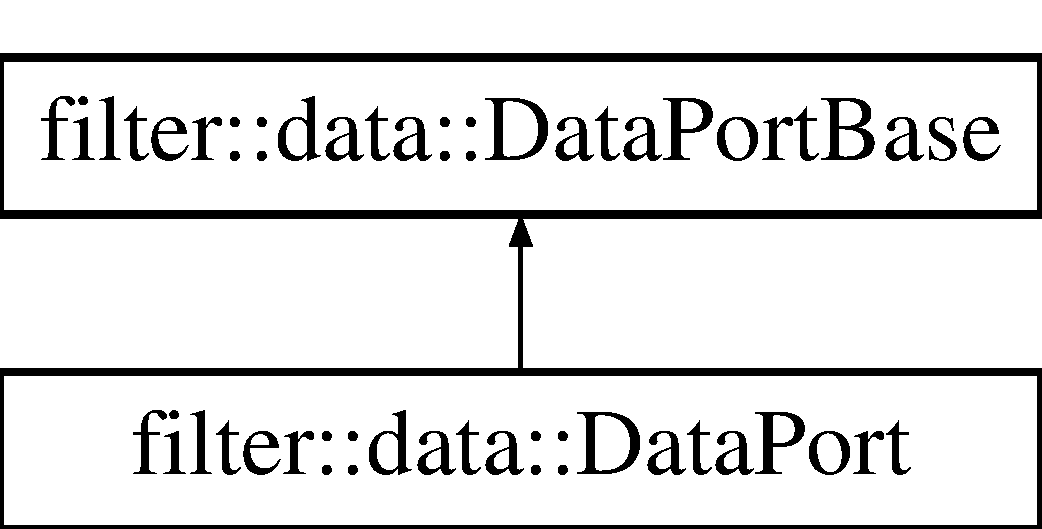
\includegraphics[height=2.000000cm]{db/dce/classfilter_1_1data_1_1_data_port_base}
\end{center}
\end{figure}


\subsection{Detailed Description}
\begin{DoxyRefDesc}{Todo}
\item[\hyperlink{todo__todo000018}{Todo}]\end{DoxyRefDesc}


The documentation for this class was generated from the following file\+:\begin{DoxyCompactItemize}
\item 
header/filter/data/Connex\+Data.\+h\end{DoxyCompactItemize}

\hypertarget{classfilter_1_1data_1_1_data_type_mapper}{}\section{filter\+:\+:data\+:\+:Data\+Type\+Mapper Class Reference}
\label{classfilter_1_1data_1_1_data_type_mapper}\index{filter\+::data\+::\+Data\+Type\+Mapper@{filter\+::data\+::\+Data\+Type\+Mapper}}
\subsection*{Static Public Member Functions}
\begin{DoxyCompactItemize}
\item 
static I\+O\+Data\+Type \hyperlink{classfilter_1_1data_1_1_data_type_mapper_afb0b4b71313e5ac7e681a8dc01518e8f}{get\+Type\+From\+String} (const std\+::string data\+Type\+String)
\begin{DoxyCompactList}\small\item\em Returns the associated. \end{DoxyCompactList}\item 
static std\+::string \hyperlink{classfilter_1_1data_1_1_data_type_mapper_a96e71517bc63d051a539162c26d17fc9}{get\+String\+From\+Type} (const I\+O\+Data\+Type \&data\+Type)
\item 
static bool \hyperlink{classfilter_1_1data_1_1_data_type_mapper_a5c2902ea638cf883f1955bfa1bebfc5e}{is\+Streaming} (const I\+O\+Data\+Type \&data\+Type)
\begin{DoxyCompactList}\small\item\em Checks if a data type is a streamed type one. \end{DoxyCompactList}\item 
static bool \hyperlink{classfilter_1_1data_1_1_data_type_mapper_acd18a509528e02426321f1d979be148c}{is\+Image} (const I\+O\+Data\+Type \&data\+Type)
\begin{DoxyCompactList}\small\item\em Checks if a data type is an image type one. \end{DoxyCompactList}\item 
static bool \hyperlink{classfilter_1_1data_1_1_data_type_mapper_ae21733c90e100f82c69455bc3ae1f2e2}{is\+Video} (const I\+O\+Data\+Type \&data\+Type)
\begin{DoxyCompactList}\small\item\em Checks if a data type is a video type one. \end{DoxyCompactList}\item 
static bool \hyperlink{classfilter_1_1data_1_1_data_type_mapper_ad4bf024b99e0a3470b8fa41523e5392c}{is\+Sequence} (const I\+O\+Data\+Type \&data\+Type)
\begin{DoxyCompactList}\small\item\em Checks if a data type is a sequence type one. \end{DoxyCompactList}\item 
static bool \hyperlink{classfilter_1_1data_1_1_data_type_mapper_a60c8bd400abf2405d068dd09851e6717}{is\+List\+Io} (const I\+O\+Data\+Type \&data\+Type)
\begin{DoxyCompactList}\small\item\em Checks if a data type is a list type one. \end{DoxyCompactList}\item 
static bool \hyperlink{classfilter_1_1data_1_1_data_type_mapper_a7ca7334cdd806a1ce9680d198a0287e6}{is\+Pattern} (const I\+O\+Data\+Type \&data\+Type)
\begin{DoxyCompactList}\small\item\em Checks if a data type is a pattern type one. \end{DoxyCompactList}\end{DoxyCompactItemize}


\subsection{Member Function Documentation}
\mbox{\Hypertarget{classfilter_1_1data_1_1_data_type_mapper_a96e71517bc63d051a539162c26d17fc9}\label{classfilter_1_1data_1_1_data_type_mapper_a96e71517bc63d051a539162c26d17fc9}} 
\index{filter\+::data\+::\+Data\+Type\+Mapper@{filter\+::data\+::\+Data\+Type\+Mapper}!get\+String\+From\+Type@{get\+String\+From\+Type}}
\index{get\+String\+From\+Type@{get\+String\+From\+Type}!filter\+::data\+::\+Data\+Type\+Mapper@{filter\+::data\+::\+Data\+Type\+Mapper}}
\subsubsection{\texorpdfstring{get\+String\+From\+Type()}{getStringFromType()}}
{\footnotesize\ttfamily static std\+::string filter\+::data\+::\+Data\+Type\+Mapper\+::get\+String\+From\+Type (\begin{DoxyParamCaption}\item[{const I\+O\+Data\+Type \&}]{data\+Type }\end{DoxyParamCaption})\hspace{0.3cm}{\ttfamily [inline]}, {\ttfamily [static]}}


\begin{DoxyParams}{Parameters}
{\em data\+Type} & An \\
\hline
\end{DoxyParams}
\begin{DoxySeeAlso}{See also}
I\+O\+Data\+Type enum value 
\end{DoxySeeAlso}
\begin{DoxyReturn}{Returns}
The name as an std\+::string object associated with 
\end{DoxyReturn}
\begin{DoxySeeAlso}{See also}
I\+O\+Data\+Type enum value 
\end{DoxySeeAlso}
\mbox{\Hypertarget{classfilter_1_1data_1_1_data_type_mapper_afb0b4b71313e5ac7e681a8dc01518e8f}\label{classfilter_1_1data_1_1_data_type_mapper_afb0b4b71313e5ac7e681a8dc01518e8f}} 
\index{filter\+::data\+::\+Data\+Type\+Mapper@{filter\+::data\+::\+Data\+Type\+Mapper}!get\+Type\+From\+String@{get\+Type\+From\+String}}
\index{get\+Type\+From\+String@{get\+Type\+From\+String}!filter\+::data\+::\+Data\+Type\+Mapper@{filter\+::data\+::\+Data\+Type\+Mapper}}
\subsubsection{\texorpdfstring{get\+Type\+From\+String()}{getTypeFromString()}}
{\footnotesize\ttfamily static I\+O\+Data\+Type filter\+::data\+::\+Data\+Type\+Mapper\+::get\+Type\+From\+String (\begin{DoxyParamCaption}\item[{const std\+::string}]{data\+Type\+String }\end{DoxyParamCaption})\hspace{0.3cm}{\ttfamily [inline]}, {\ttfamily [static]}}

\begin{DoxySeeAlso}{See also}
I\+O\+Data\+Type enum value from its corresponding name in text 
\end{DoxySeeAlso}

\begin{DoxyParams}{Parameters}
{\em data\+Type\+String} & The name of the requested data type \\
\hline
\end{DoxyParams}
\begin{DoxyReturn}{Returns}
The data type as an 
\end{DoxyReturn}
\begin{DoxySeeAlso}{See also}
I\+O\+Data\+Type enum value 
\end{DoxySeeAlso}
\mbox{\Hypertarget{classfilter_1_1data_1_1_data_type_mapper_acd18a509528e02426321f1d979be148c}\label{classfilter_1_1data_1_1_data_type_mapper_acd18a509528e02426321f1d979be148c}} 
\index{filter\+::data\+::\+Data\+Type\+Mapper@{filter\+::data\+::\+Data\+Type\+Mapper}!is\+Image@{is\+Image}}
\index{is\+Image@{is\+Image}!filter\+::data\+::\+Data\+Type\+Mapper@{filter\+::data\+::\+Data\+Type\+Mapper}}
\subsubsection{\texorpdfstring{is\+Image()}{isImage()}}
{\footnotesize\ttfamily static bool filter\+::data\+::\+Data\+Type\+Mapper\+::is\+Image (\begin{DoxyParamCaption}\item[{const I\+O\+Data\+Type \&}]{data\+Type }\end{DoxyParamCaption})\hspace{0.3cm}{\ttfamily [inline]}, {\ttfamily [static]}}


\begin{DoxyParams}{Parameters}
{\em data\+Type} & The queried data type \\
\hline
\end{DoxyParams}
\begin{DoxyReturn}{Returns}
Returns true if the queried data type is an image type one 
\end{DoxyReturn}
\mbox{\Hypertarget{classfilter_1_1data_1_1_data_type_mapper_a60c8bd400abf2405d068dd09851e6717}\label{classfilter_1_1data_1_1_data_type_mapper_a60c8bd400abf2405d068dd09851e6717}} 
\index{filter\+::data\+::\+Data\+Type\+Mapper@{filter\+::data\+::\+Data\+Type\+Mapper}!is\+List\+Io@{is\+List\+Io}}
\index{is\+List\+Io@{is\+List\+Io}!filter\+::data\+::\+Data\+Type\+Mapper@{filter\+::data\+::\+Data\+Type\+Mapper}}
\subsubsection{\texorpdfstring{is\+List\+Io()}{isListIo()}}
{\footnotesize\ttfamily static bool filter\+::data\+::\+Data\+Type\+Mapper\+::is\+List\+Io (\begin{DoxyParamCaption}\item[{const I\+O\+Data\+Type \&}]{data\+Type }\end{DoxyParamCaption})\hspace{0.3cm}{\ttfamily [inline]}, {\ttfamily [static]}}


\begin{DoxyParams}{Parameters}
{\em data\+Type} & The queried data type \\
\hline
\end{DoxyParams}
\begin{DoxyReturn}{Returns}
Returns true if the queried data type is a list type one 
\end{DoxyReturn}
\mbox{\Hypertarget{classfilter_1_1data_1_1_data_type_mapper_a7ca7334cdd806a1ce9680d198a0287e6}\label{classfilter_1_1data_1_1_data_type_mapper_a7ca7334cdd806a1ce9680d198a0287e6}} 
\index{filter\+::data\+::\+Data\+Type\+Mapper@{filter\+::data\+::\+Data\+Type\+Mapper}!is\+Pattern@{is\+Pattern}}
\index{is\+Pattern@{is\+Pattern}!filter\+::data\+::\+Data\+Type\+Mapper@{filter\+::data\+::\+Data\+Type\+Mapper}}
\subsubsection{\texorpdfstring{is\+Pattern()}{isPattern()}}
{\footnotesize\ttfamily static bool filter\+::data\+::\+Data\+Type\+Mapper\+::is\+Pattern (\begin{DoxyParamCaption}\item[{const I\+O\+Data\+Type \&}]{data\+Type }\end{DoxyParamCaption})\hspace{0.3cm}{\ttfamily [inline]}, {\ttfamily [static]}}


\begin{DoxyParams}{Parameters}
{\em data\+Type} & The queried data type \\
\hline
\end{DoxyParams}
\begin{DoxyReturn}{Returns}
Returns true if the queried data type is a pattern type one 
\end{DoxyReturn}
\mbox{\Hypertarget{classfilter_1_1data_1_1_data_type_mapper_ad4bf024b99e0a3470b8fa41523e5392c}\label{classfilter_1_1data_1_1_data_type_mapper_ad4bf024b99e0a3470b8fa41523e5392c}} 
\index{filter\+::data\+::\+Data\+Type\+Mapper@{filter\+::data\+::\+Data\+Type\+Mapper}!is\+Sequence@{is\+Sequence}}
\index{is\+Sequence@{is\+Sequence}!filter\+::data\+::\+Data\+Type\+Mapper@{filter\+::data\+::\+Data\+Type\+Mapper}}
\subsubsection{\texorpdfstring{is\+Sequence()}{isSequence()}}
{\footnotesize\ttfamily static bool filter\+::data\+::\+Data\+Type\+Mapper\+::is\+Sequence (\begin{DoxyParamCaption}\item[{const I\+O\+Data\+Type \&}]{data\+Type }\end{DoxyParamCaption})\hspace{0.3cm}{\ttfamily [inline]}, {\ttfamily [static]}}


\begin{DoxyParams}{Parameters}
{\em data\+Type} & The queried data type \\
\hline
\end{DoxyParams}
\begin{DoxyReturn}{Returns}
Returns true if the queried data type is a sequence type one 
\end{DoxyReturn}
\mbox{\Hypertarget{classfilter_1_1data_1_1_data_type_mapper_a5c2902ea638cf883f1955bfa1bebfc5e}\label{classfilter_1_1data_1_1_data_type_mapper_a5c2902ea638cf883f1955bfa1bebfc5e}} 
\index{filter\+::data\+::\+Data\+Type\+Mapper@{filter\+::data\+::\+Data\+Type\+Mapper}!is\+Streaming@{is\+Streaming}}
\index{is\+Streaming@{is\+Streaming}!filter\+::data\+::\+Data\+Type\+Mapper@{filter\+::data\+::\+Data\+Type\+Mapper}}
\subsubsection{\texorpdfstring{is\+Streaming()}{isStreaming()}}
{\footnotesize\ttfamily static bool filter\+::data\+::\+Data\+Type\+Mapper\+::is\+Streaming (\begin{DoxyParamCaption}\item[{const I\+O\+Data\+Type \&}]{data\+Type }\end{DoxyParamCaption})\hspace{0.3cm}{\ttfamily [inline]}, {\ttfamily [static]}}


\begin{DoxyParams}{Parameters}
{\em data\+Type} & The queried data type \\
\hline
\end{DoxyParams}
\begin{DoxyReturn}{Returns}
Returns true if the queried data type is a streaming type one 
\end{DoxyReturn}
\mbox{\Hypertarget{classfilter_1_1data_1_1_data_type_mapper_ae21733c90e100f82c69455bc3ae1f2e2}\label{classfilter_1_1data_1_1_data_type_mapper_ae21733c90e100f82c69455bc3ae1f2e2}} 
\index{filter\+::data\+::\+Data\+Type\+Mapper@{filter\+::data\+::\+Data\+Type\+Mapper}!is\+Video@{is\+Video}}
\index{is\+Video@{is\+Video}!filter\+::data\+::\+Data\+Type\+Mapper@{filter\+::data\+::\+Data\+Type\+Mapper}}
\subsubsection{\texorpdfstring{is\+Video()}{isVideo()}}
{\footnotesize\ttfamily static bool filter\+::data\+::\+Data\+Type\+Mapper\+::is\+Video (\begin{DoxyParamCaption}\item[{const I\+O\+Data\+Type \&}]{data\+Type }\end{DoxyParamCaption})\hspace{0.3cm}{\ttfamily [inline]}, {\ttfamily [static]}}


\begin{DoxyParams}{Parameters}
{\em data\+Type} & The queried data type \\
\hline
\end{DoxyParams}
\begin{DoxyReturn}{Returns}
Returns true if the queried data type is a video type one 
\end{DoxyReturn}


The documentation for this class was generated from the following file\+:\begin{DoxyCompactItemize}
\item 
header/filter/data/I\+O\+Data\+Type.\+h\end{DoxyCompactItemize}

\hypertarget{classorchestrator_1_1image_1_1_default_scheduler}{}\section{orchestrator\+:\+:image\+:\+:Default\+Scheduler Class Reference}
\label{classorchestrator_1_1image_1_1_default_scheduler}\index{orchestrator\+::image\+::\+Default\+Scheduler@{orchestrator\+::image\+::\+Default\+Scheduler}}
Inheritance diagram for orchestrator\+:\+:image\+:\+:Default\+Scheduler\+:\begin{figure}[H]
\begin{center}
\leavevmode
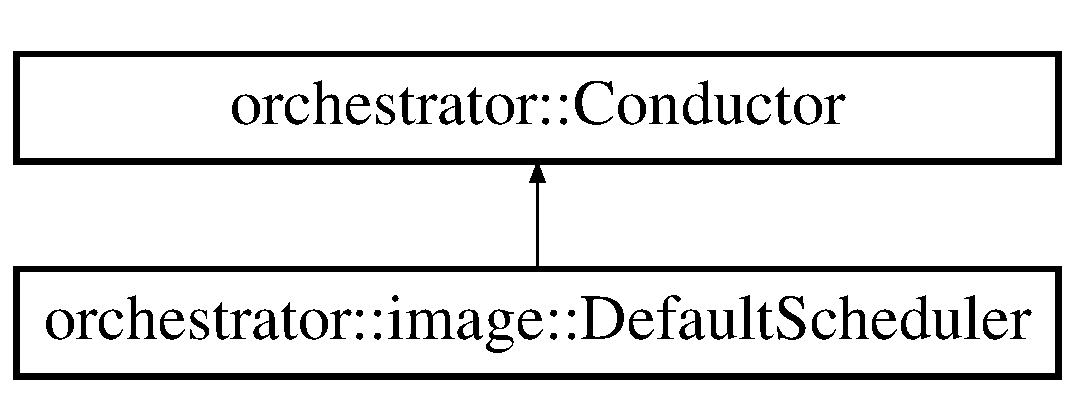
\includegraphics[height=2.000000cm]{d9/d04/classorchestrator_1_1image_1_1_default_scheduler}
\end{center}
\end{figure}
\subsection*{Public Types}
\begin{DoxyCompactItemize}
\item 
\mbox{\Hypertarget{classorchestrator_1_1image_1_1_default_scheduler_a050a53553d53c862899d7ac75acb7bb7}\label{classorchestrator_1_1image_1_1_default_scheduler_a050a53553d53c862899d7ac75acb7bb7}} 
typedef std\+::vector$<$ std\+::vector$<$ \hyperlink{classfilter_1_1_model}{filter\+::\+Model} $\ast$ $>$ $>$ {\bfseries Matrix\+Layer\+Node}
\end{DoxyCompactItemize}
\subsection*{Public Member Functions}
\begin{DoxyCompactItemize}
\item 
\mbox{\Hypertarget{classorchestrator_1_1image_1_1_default_scheduler_abe112bc7fd8d4e9cbf3e40aa0b99d621}\label{classorchestrator_1_1image_1_1_default_scheduler_abe112bc7fd8d4e9cbf3e40aa0b99d621}} 
void {\bfseries process\+Streaming} (\hyperlink{classfilter_1_1_model}{filter\+::\+Model} $\ast$root, \hyperlink{classfilter_1_1data_1_1_data}{filter\+::data\+::\+Data} \&input\+Data, \hyperlink{classfilter_1_1data_1_1_data}{filter\+::data\+::\+Data} \&output\+Data, bool debug)
\item 
\mbox{\Hypertarget{classorchestrator_1_1image_1_1_default_scheduler_ad257f9697cc5158ca1bee71c36514dd7}\label{classorchestrator_1_1image_1_1_default_scheduler_ad257f9697cc5158ca1bee71c36514dd7}} 
{\footnotesize template$<$class Video\+Class $>$ }\\void {\bfseries process\+Video} (\hyperlink{classfilter_1_1_model}{filter\+::\+Model} $\ast$root, Video\+Class \&input\+Data, \hyperlink{classfilter_1_1data_1_1_data}{filter\+::data\+::\+Data} \&output\+Data, bool debug)
\item 
\mbox{\Hypertarget{classorchestrator_1_1image_1_1_default_scheduler_a6308d4fe7856fd9c05844a183b98b36e}\label{classorchestrator_1_1image_1_1_default_scheduler_a6308d4fe7856fd9c05844a183b98b36e}} 
void {\bfseries process\+Sequence} (\hyperlink{classfilter_1_1_model}{filter\+::\+Model} $\ast$root, \hyperlink{classfilter_1_1data_1_1_data}{filter\+::data\+::\+Data} \&input\+Data, \hyperlink{classfilter_1_1data_1_1_data}{filter\+::data\+::\+Data} \&output\+Data, bool debug)
\item 
\mbox{\Hypertarget{classorchestrator_1_1image_1_1_default_scheduler_a1f91904098a71297914e2591ba07c938}\label{classorchestrator_1_1image_1_1_default_scheduler_a1f91904098a71297914e2591ba07c938}} 
void {\bfseries process\+List\+Data} (\hyperlink{classfilter_1_1_model}{filter\+::\+Model} $\ast$root, \hyperlink{classfilter_1_1data_1_1_list_i_o_data}{filter\+::data\+::\+List\+I\+O\+Data} \&input\+Data, \hyperlink{classfilter_1_1data_1_1_data}{filter\+::data\+::\+Data} \&output\+Data, bool debug)
\item 
\mbox{\Hypertarget{classorchestrator_1_1image_1_1_default_scheduler_a51179bf83b16153f2b7eb13b7af6c22c}\label{classorchestrator_1_1image_1_1_default_scheduler_a51179bf83b16153f2b7eb13b7af6c22c}} 
void {\bfseries process\+Images} (\hyperlink{classfilter_1_1_model}{filter\+::\+Model} $\ast$root, \hyperlink{classfilter_1_1data_1_1_data}{filter\+::data\+::\+Data} \&input\+Data, \hyperlink{classfilter_1_1data_1_1_data}{filter\+::data\+::\+Data} \&output\+Data, bool debug)
\item 
\mbox{\Hypertarget{classorchestrator_1_1image_1_1_default_scheduler_ac3f702904a59c02604088e836bae8c33}\label{classorchestrator_1_1image_1_1_default_scheduler_ac3f702904a59c02604088e836bae8c33}} 
void {\bfseries process\+Pattern} (\hyperlink{classfilter_1_1_model}{filter\+::\+Model} $\ast$root, \hyperlink{classfilter_1_1data_1_1_data}{filter\+::data\+::\+Data} data, \hyperlink{classfilter_1_1data_1_1_data}{filter\+::data\+::\+Data} \&output\+\_\+data, bool debug)
\item 
\mbox{\Hypertarget{classorchestrator_1_1image_1_1_default_scheduler_a4d6d533550cadc8852d24672b7669be3}\label{classorchestrator_1_1image_1_1_default_scheduler_a4d6d533550cadc8852d24672b7669be3}} 
void {\bfseries process} (\hyperlink{classfilter_1_1_model}{filter\+::\+Model} $\ast$root, \hyperlink{classfilter_1_1data_1_1_data}{filter\+::data\+::\+Data} \&input\+Data, \hyperlink{classfilter_1_1data_1_1_data}{filter\+::data\+::\+Data} \&output\+Data, bool debug=false)
\item 
\mbox{\Hypertarget{classorchestrator_1_1image_1_1_default_scheduler_addd713281367b509cf393463ece3c709}\label{classorchestrator_1_1image_1_1_default_scheduler_addd713281367b509cf393463ece3c709}} 
virtual void {\bfseries killall} ()
\end{DoxyCompactItemize}
\subsection*{Static Public Member Functions}
\begin{DoxyCompactItemize}
\item 
\mbox{\Hypertarget{classorchestrator_1_1image_1_1_default_scheduler_aff1a90d0a46fc1a7dfab983a34d273fb}\label{classorchestrator_1_1image_1_1_default_scheduler_aff1a90d0a46fc1a7dfab983a34d273fb}} 
static int {\bfseries get\+Max\+Level\+Node} (\hyperlink{classfilter_1_1_model}{filter\+::\+Model} $\ast$filter, int level=0)
\item 
\mbox{\Hypertarget{classorchestrator_1_1image_1_1_default_scheduler_a09d8b17733aabc9916483815df482a09}\label{classorchestrator_1_1image_1_1_default_scheduler_a09d8b17733aabc9916483815df482a09}} 
static int {\bfseries set\+Matrix\+Layer} (\hyperlink{classfilter_1_1_model}{filter\+::\+Model} $\ast$filter, Matrix\+Layer\+Node \&matrix\+Layer\+Node)
\item 
\mbox{\Hypertarget{classorchestrator_1_1image_1_1_default_scheduler_ac0a1cc8c42f8d8ddd2753981058ba5ce}\label{classorchestrator_1_1image_1_1_default_scheduler_ac0a1cc8c42f8d8ddd2753981058ba5ce}} 
static void {\bfseries clean\+Data\+Child} (\hyperlink{classfilter_1_1_model}{filter\+::\+Model} $\ast$filter)
\item 
\mbox{\Hypertarget{classorchestrator_1_1image_1_1_default_scheduler_a32a61ca9287fb07762810989a4fc316f}\label{classorchestrator_1_1image_1_1_default_scheduler_a32a61ca9287fb07762810989a4fc316f}} 
static void {\bfseries dispose\+Child} (\hyperlink{classfilter_1_1_model}{filter\+::\+Model} $\ast$filter)
\end{DoxyCompactItemize}
\subsection*{Public Attributes}
\begin{DoxyCompactItemize}
\item 
\mbox{\Hypertarget{classorchestrator_1_1image_1_1_default_scheduler_ad14f430cc24d129353b21c7df3e28ceb}\label{classorchestrator_1_1image_1_1_default_scheduler_ad14f430cc24d129353b21c7df3e28ceb}} 
std\+::vector$<$ \hyperlink{classorchestrator_1_1_task_info}{Task\+Info} $>$ {\bfseries running\+Tasks}
\end{DoxyCompactItemize}


The documentation for this class was generated from the following file\+:\begin{DoxyCompactItemize}
\item 
header/orchestrator/image/Default\+Scheduler.\+h\end{DoxyCompactItemize}

\hypertarget{class_delegate}{}\section{Delegate$<$ return\+\_\+type, params $>$ Class Template Reference}
\label{class_delegate}\index{Delegate$<$ return\+\_\+type, params $>$@{Delegate$<$ return\+\_\+type, params $>$}}
\subsection*{Public Member Functions}
\begin{DoxyCompactItemize}
\item 
\mbox{\Hypertarget{class_delegate_a77fbd96d81a622da70a9cd278fa8a90e}\label{class_delegate_a77fbd96d81a622da70a9cd278fa8a90e}} 
{\bfseries Delegate} (void $\ast$callee, Type function)
\item 
\mbox{\Hypertarget{class_delegate_a3e82d4b647fddf4686c4d8c66f27708a}\label{class_delegate_a3e82d4b647fddf4686c4d8c66f27708a}} 
return\+\_\+type {\bfseries operator()} (params... xs) const
\end{DoxyCompactItemize}
\subsection*{Static Public Member Functions}
\begin{DoxyCompactItemize}
\item 
\mbox{\Hypertarget{class_delegate_aa116b260be972435ef89d480c7df8b09}\label{class_delegate_aa116b260be972435ef89d480c7df8b09}} 
{\footnotesize template$<$class T , return\+\_\+type(\+T\+::$\ast$)(params...) T\+Method$>$ }\\static \hyperlink{class_delegate}{Delegate} {\bfseries from\+\_\+function} (T $\ast$callee)
\end{DoxyCompactItemize}
\subsection*{Private Types}
\begin{DoxyCompactItemize}
\item 
\mbox{\Hypertarget{class_delegate_aa173a088403e41fdadeb32c4a14861f3}\label{class_delegate_aa173a088403e41fdadeb32c4a14861f3}} 
typedef return\+\_\+type($\ast$ {\bfseries Type}) (void $\ast$callee, params...)
\end{DoxyCompactItemize}
\subsection*{Static Private Member Functions}
\begin{DoxyCompactItemize}
\item 
\mbox{\Hypertarget{class_delegate_ace9d3fa55fab2c6b0766de9e3bbd1776}\label{class_delegate_ace9d3fa55fab2c6b0766de9e3bbd1776}} 
{\footnotesize template$<$class T , return\+\_\+type(\+T\+::$\ast$)(params...) T\+Method$>$ }\\static return\+\_\+type {\bfseries method\+Caller} (void $\ast$callee, params... xs)
\end{DoxyCompactItemize}
\subsection*{Private Attributes}
\begin{DoxyCompactItemize}
\item 
\mbox{\Hypertarget{class_delegate_ac006440f17274562043965efe6d3132c}\label{class_delegate_ac006440f17274562043965efe6d3132c}} 
void $\ast$ {\bfseries fp\+Callee}
\item 
\mbox{\Hypertarget{class_delegate_a8c788b809ab07fd5791d8b42d0a24d7c}\label{class_delegate_a8c788b809ab07fd5791d8b42d0a24d7c}} 
Type {\bfseries fp\+Callback\+Function}
\end{DoxyCompactItemize}


The documentation for this class was generated from the following file\+:\begin{DoxyCompactItemize}
\item 
header/core/Delegate.\+h\end{DoxyCompactItemize}

\hypertarget{classfilter_1_1algos_1_1_dilate}{}\section{filter\+:\+:algos\+:\+:Dilate Class Reference}
\label{classfilter_1_1algos_1_1_dilate}\index{filter\+::algos\+::\+Dilate@{filter\+::algos\+::\+Dilate}}
Inheritance diagram for filter\+:\+:algos\+:\+:Dilate\+:\begin{figure}[H]
\begin{center}
\leavevmode
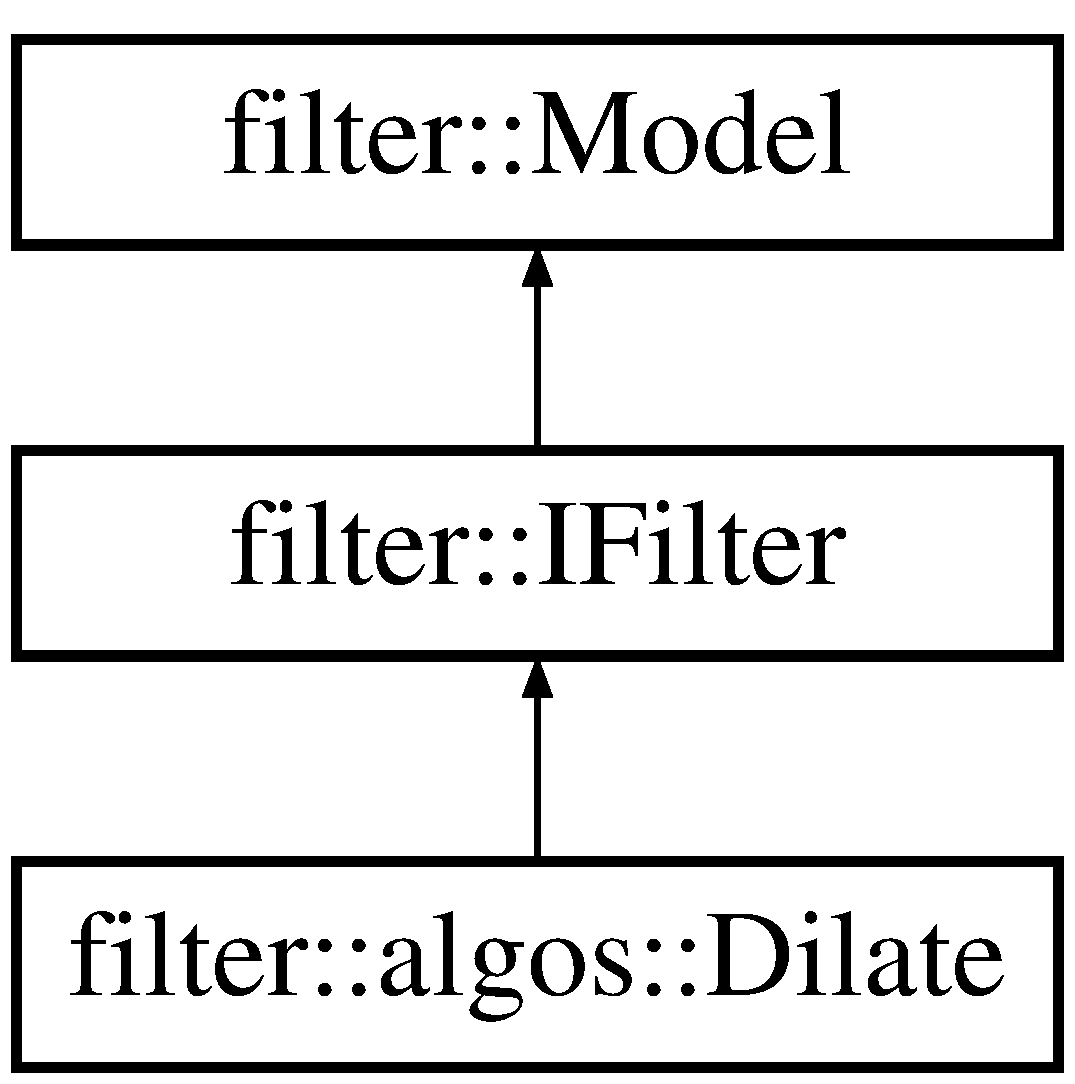
\includegraphics[height=3.000000cm]{de/de2/classfilter_1_1algos_1_1_dilate}
\end{center}
\end{figure}
\subsection*{Public Types}
\begin{DoxyCompactItemize}
\item 
\mbox{\Hypertarget{classfilter_1_1algos_1_1_dilate_af05fbd11aac2914a073e123f6a6a06d0}\label{classfilter_1_1algos_1_1_dilate_af05fbd11aac2914a073e123f6a6a06d0}} 
typedef \hyperlink{class_proxy_functor}{Proxy\+Functor}$<$ \hyperlink{classfilter_1_1algos_1_1_dilate}{Dilate} $>$ {\bfseries \+\_\+proxy\+Functor}
\item 
\mbox{\Hypertarget{classfilter_1_1algos_1_1_dilate_a115326e512d434599bf888c9c22691a2}\label{classfilter_1_1algos_1_1_dilate_a115326e512d434599bf888c9c22691a2}} 
typedef \hyperlink{classfilter_1_1algos_1_1_dilate}{Dilate} {\bfseries mytype}
\item 
\mbox{\Hypertarget{classfilter_1_1algos_1_1_dilate_af5c6fbbaddce7209a735bfaa9945fa03}\label{classfilter_1_1algos_1_1_dilate_af5c6fbbaddce7209a735bfaa9945fa03}} 
typedef int {\bfseries vartype\+\_\+\+\_\+iterations}
\item 
\mbox{\Hypertarget{classfilter_1_1algos_1_1_dilate_a9258cacda0e613d4af72945ee2662226}\label{classfilter_1_1algos_1_1_dilate_a9258cacda0e613d4af72945ee2662226}} 
typedef std\+::string {\bfseries vartype\+\_\+\+\_\+morph\+Type}
\item 
\mbox{\Hypertarget{classfilter_1_1algos_1_1_dilate_ae385a0384b35ddc0606fe4a9dfc2327a}\label{classfilter_1_1algos_1_1_dilate_ae385a0384b35ddc0606fe4a9dfc2327a}} 
typedef std\+::string {\bfseries vartype\+\_\+\+\_\+morph\+Shape}
\item 
\mbox{\Hypertarget{classfilter_1_1algos_1_1_dilate_a6715cde74d38cb990188c092ffd981cf}\label{classfilter_1_1algos_1_1_dilate_a6715cde74d38cb990188c092ffd981cf}} 
typedef int {\bfseries vartype\+\_\+\+\_\+kernel\+SizeX}
\item 
\mbox{\Hypertarget{classfilter_1_1algos_1_1_dilate_ad1abfbcfd400fcf28bee4e4a083c6a4c}\label{classfilter_1_1algos_1_1_dilate_ad1abfbcfd400fcf28bee4e4a083c6a4c}} 
typedef int {\bfseries vartype\+\_\+\+\_\+kernel\+SizeY}
\item 
\mbox{\Hypertarget{classfilter_1_1algos_1_1_dilate_afecc3fa88157ebc3e66e610590397461}\label{classfilter_1_1algos_1_1_dilate_afecc3fa88157ebc3e66e610590397461}} 
typedef int {\bfseries vartype\+\_\+\+\_\+anchorX}
\item 
\mbox{\Hypertarget{classfilter_1_1algos_1_1_dilate_adde43e4c66e7f89982d9a050bf8760d2}\label{classfilter_1_1algos_1_1_dilate_adde43e4c66e7f89982d9a050bf8760d2}} 
typedef int {\bfseries vartype\+\_\+\+\_\+anchorY}
\end{DoxyCompactItemize}
\subsection*{Public Member Functions}
\begin{DoxyCompactItemize}
\item 
\mbox{\Hypertarget{classfilter_1_1algos_1_1_dilate_acaf2aae04ee7e94bfd85f934efcc434b}\label{classfilter_1_1algos_1_1_dilate_acaf2aae04ee7e94bfd85f934efcc434b}} 
void {\bfseries set\+\_\+iterations\+\_\+from\+\_\+json} (boost\+::property\+\_\+tree\+::ptree \&json\+Class)
\item 
\mbox{\Hypertarget{classfilter_1_1algos_1_1_dilate_af91a78e1f1318aa33613ff1a7982dc91}\label{classfilter_1_1algos_1_1_dilate_af91a78e1f1318aa33613ff1a7982dc91}} 
void {\bfseries set\+\_\+iterations} (vartype\+\_\+\+\_\+iterations \&\+\_\+\+\_\+iterations)
\item 
\mbox{\Hypertarget{classfilter_1_1algos_1_1_dilate_ad35efc44f44e92504bd19cd6bfb09493}\label{classfilter_1_1algos_1_1_dilate_ad35efc44f44e92504bd19cd6bfb09493}} 
vartype\+\_\+\+\_\+iterations {\bfseries get\+\_\+iterations} ()
\item 
\mbox{\Hypertarget{classfilter_1_1algos_1_1_dilate_ad2a9c72c42ae8562466e4d2c43fe2d25}\label{classfilter_1_1algos_1_1_dilate_ad2a9c72c42ae8562466e4d2c43fe2d25}} 
void {\bfseries copy\+\_\+iterations} (\hyperlink{classfilter_1_1algos_1_1_dilate}{mytype} $\ast$instance)
\item 
\mbox{\Hypertarget{classfilter_1_1algos_1_1_dilate_a7f22d5d9a9e9588c5d64f581646d8007}\label{classfilter_1_1algos_1_1_dilate_a7f22d5d9a9e9588c5d64f581646d8007}} 
void {\bfseries set\+\_\+morph\+Type\+\_\+from\+\_\+json} (boost\+::property\+\_\+tree\+::ptree \&json\+Class)
\item 
\mbox{\Hypertarget{classfilter_1_1algos_1_1_dilate_a341a79c5a7c8d6a076d649144dd26a68}\label{classfilter_1_1algos_1_1_dilate_a341a79c5a7c8d6a076d649144dd26a68}} 
void {\bfseries set\+\_\+morph\+Type} (vartype\+\_\+\+\_\+morph\+Type \&\+\_\+\+\_\+morph\+Type)
\item 
\mbox{\Hypertarget{classfilter_1_1algos_1_1_dilate_a0eba06ba1158da3b9842dbab788da270}\label{classfilter_1_1algos_1_1_dilate_a0eba06ba1158da3b9842dbab788da270}} 
vartype\+\_\+\+\_\+morph\+Type {\bfseries get\+\_\+morph\+Type} ()
\item 
\mbox{\Hypertarget{classfilter_1_1algos_1_1_dilate_ad5ad3caafe560330bb33d4817095ca04}\label{classfilter_1_1algos_1_1_dilate_ad5ad3caafe560330bb33d4817095ca04}} 
void {\bfseries copy\+\_\+morph\+Type} (\hyperlink{classfilter_1_1algos_1_1_dilate}{mytype} $\ast$instance)
\item 
\mbox{\Hypertarget{classfilter_1_1algos_1_1_dilate_a349038c6c0380dbc3f6f04d2d6e47bcb}\label{classfilter_1_1algos_1_1_dilate_a349038c6c0380dbc3f6f04d2d6e47bcb}} 
void {\bfseries set\+\_\+morph\+Shape\+\_\+from\+\_\+json} (boost\+::property\+\_\+tree\+::ptree \&json\+Class)
\item 
\mbox{\Hypertarget{classfilter_1_1algos_1_1_dilate_a512fcacd934ac8fd6d76c82dcf4ce8a9}\label{classfilter_1_1algos_1_1_dilate_a512fcacd934ac8fd6d76c82dcf4ce8a9}} 
void {\bfseries set\+\_\+morph\+Shape} (vartype\+\_\+\+\_\+morph\+Shape \&\+\_\+\+\_\+morph\+Shape)
\item 
\mbox{\Hypertarget{classfilter_1_1algos_1_1_dilate_af4f1e99014e2e733ff3924db5be2b240}\label{classfilter_1_1algos_1_1_dilate_af4f1e99014e2e733ff3924db5be2b240}} 
vartype\+\_\+\+\_\+morph\+Shape {\bfseries get\+\_\+morph\+Shape} ()
\item 
\mbox{\Hypertarget{classfilter_1_1algos_1_1_dilate_a9ad0a58e202b3e4de86336413b46d062}\label{classfilter_1_1algos_1_1_dilate_a9ad0a58e202b3e4de86336413b46d062}} 
void {\bfseries copy\+\_\+morph\+Shape} (\hyperlink{classfilter_1_1algos_1_1_dilate}{mytype} $\ast$instance)
\item 
\mbox{\Hypertarget{classfilter_1_1algos_1_1_dilate_a75feddb586e15d6b686405bfedc7c27c}\label{classfilter_1_1algos_1_1_dilate_a75feddb586e15d6b686405bfedc7c27c}} 
void {\bfseries set\+\_\+kernel\+Size\+X\+\_\+from\+\_\+json} (boost\+::property\+\_\+tree\+::ptree \&json\+Class)
\item 
\mbox{\Hypertarget{classfilter_1_1algos_1_1_dilate_ad5261f0c94b0fa43e982deadf5c3cdb0}\label{classfilter_1_1algos_1_1_dilate_ad5261f0c94b0fa43e982deadf5c3cdb0}} 
void {\bfseries set\+\_\+kernel\+SizeX} (vartype\+\_\+\+\_\+kernel\+SizeX \&\+\_\+\+\_\+kernel\+SizeX)
\item 
\mbox{\Hypertarget{classfilter_1_1algos_1_1_dilate_af5dbbd622edbc6f492ef8991dea98e49}\label{classfilter_1_1algos_1_1_dilate_af5dbbd622edbc6f492ef8991dea98e49}} 
vartype\+\_\+\+\_\+kernel\+SizeX {\bfseries get\+\_\+kernel\+SizeX} ()
\item 
\mbox{\Hypertarget{classfilter_1_1algos_1_1_dilate_a6a79def683c8acd90b96bf3cb8744929}\label{classfilter_1_1algos_1_1_dilate_a6a79def683c8acd90b96bf3cb8744929}} 
void {\bfseries copy\+\_\+kernel\+SizeX} (\hyperlink{classfilter_1_1algos_1_1_dilate}{mytype} $\ast$instance)
\item 
\mbox{\Hypertarget{classfilter_1_1algos_1_1_dilate_a778b8d199af54072cd1401773f2afc99}\label{classfilter_1_1algos_1_1_dilate_a778b8d199af54072cd1401773f2afc99}} 
void {\bfseries set\+\_\+kernel\+Size\+Y\+\_\+from\+\_\+json} (boost\+::property\+\_\+tree\+::ptree \&json\+Class)
\item 
\mbox{\Hypertarget{classfilter_1_1algos_1_1_dilate_aa8664f36d3f5f1ed9d89f5860ec6b01d}\label{classfilter_1_1algos_1_1_dilate_aa8664f36d3f5f1ed9d89f5860ec6b01d}} 
void {\bfseries set\+\_\+kernel\+SizeY} (vartype\+\_\+\+\_\+kernel\+SizeY \&\+\_\+\+\_\+kernel\+SizeY)
\item 
\mbox{\Hypertarget{classfilter_1_1algos_1_1_dilate_a6534c28d28630ac3e701b4d55735bb73}\label{classfilter_1_1algos_1_1_dilate_a6534c28d28630ac3e701b4d55735bb73}} 
vartype\+\_\+\+\_\+kernel\+SizeY {\bfseries get\+\_\+kernel\+SizeY} ()
\item 
\mbox{\Hypertarget{classfilter_1_1algos_1_1_dilate_a6e17d2ebc1bf6abb4bc166b201fb3b7a}\label{classfilter_1_1algos_1_1_dilate_a6e17d2ebc1bf6abb4bc166b201fb3b7a}} 
void {\bfseries copy\+\_\+kernel\+SizeY} (\hyperlink{classfilter_1_1algos_1_1_dilate}{mytype} $\ast$instance)
\item 
\mbox{\Hypertarget{classfilter_1_1algos_1_1_dilate_aa0c40a0e409d206154f4fe9250579fc0}\label{classfilter_1_1algos_1_1_dilate_aa0c40a0e409d206154f4fe9250579fc0}} 
void {\bfseries set\+\_\+anchor\+X\+\_\+from\+\_\+json} (boost\+::property\+\_\+tree\+::ptree \&json\+Class)
\item 
\mbox{\Hypertarget{classfilter_1_1algos_1_1_dilate_aa36b71d9387b6a1166047caa6d507b76}\label{classfilter_1_1algos_1_1_dilate_aa36b71d9387b6a1166047caa6d507b76}} 
void {\bfseries set\+\_\+anchorX} (vartype\+\_\+\+\_\+anchorX \&\+\_\+\+\_\+anchorX)
\item 
\mbox{\Hypertarget{classfilter_1_1algos_1_1_dilate_a5750b340c8d34d3b8c951d578f52bdc9}\label{classfilter_1_1algos_1_1_dilate_a5750b340c8d34d3b8c951d578f52bdc9}} 
vartype\+\_\+\+\_\+anchorX {\bfseries get\+\_\+anchorX} ()
\item 
\mbox{\Hypertarget{classfilter_1_1algos_1_1_dilate_ad68b6e29e30614c9131c019157db50b8}\label{classfilter_1_1algos_1_1_dilate_ad68b6e29e30614c9131c019157db50b8}} 
void {\bfseries copy\+\_\+anchorX} (\hyperlink{classfilter_1_1algos_1_1_dilate}{mytype} $\ast$instance)
\item 
\mbox{\Hypertarget{classfilter_1_1algos_1_1_dilate_ae9e267ebb6d66de1cd7f38e512cbab3e}\label{classfilter_1_1algos_1_1_dilate_ae9e267ebb6d66de1cd7f38e512cbab3e}} 
void {\bfseries set\+\_\+anchor\+Y\+\_\+from\+\_\+json} (boost\+::property\+\_\+tree\+::ptree \&json\+Class)
\item 
\mbox{\Hypertarget{classfilter_1_1algos_1_1_dilate_a556a9d1d1127e3c6dd6b3e1adb8d939a}\label{classfilter_1_1algos_1_1_dilate_a556a9d1d1127e3c6dd6b3e1adb8d939a}} 
void {\bfseries set\+\_\+anchorY} (vartype\+\_\+\+\_\+anchorY \&\+\_\+\+\_\+anchorY)
\item 
\mbox{\Hypertarget{classfilter_1_1algos_1_1_dilate_afd4ff295f7e801ee88a77dda956b7a26}\label{classfilter_1_1algos_1_1_dilate_afd4ff295f7e801ee88a77dda956b7a26}} 
vartype\+\_\+\+\_\+anchorY {\bfseries get\+\_\+anchorY} ()
\item 
\mbox{\Hypertarget{classfilter_1_1algos_1_1_dilate_a51a3feb6d21f46877e740ea7deda8380}\label{classfilter_1_1algos_1_1_dilate_a51a3feb6d21f46877e740ea7deda8380}} 
void {\bfseries copy\+\_\+anchorY} (\hyperlink{classfilter_1_1algos_1_1_dilate}{mytype} $\ast$instance)
\item 
\mbox{\Hypertarget{classfilter_1_1algos_1_1_dilate_ac35eac6b1fe8a370b2315f9692785533}\label{classfilter_1_1algos_1_1_dilate_ac35eac6b1fe8a370b2315f9692785533}} 
Hipe\+Status {\bfseries process} () override
\end{DoxyCompactItemize}
\subsection*{Public Attributes}
\begin{DoxyCompactItemize}
\item 
\mbox{\Hypertarget{classfilter_1_1algos_1_1_dilate_abbaed4fd63964a534c40eb0a27333151}\label{classfilter_1_1algos_1_1_dilate_abbaed4fd63964a534c40eb0a27333151}} 
int {\bfseries iterations}
\item 
\mbox{\Hypertarget{classfilter_1_1algos_1_1_dilate_aaddee9ad24724a9b85b87e3b1f44a355}\label{classfilter_1_1algos_1_1_dilate_aaddee9ad24724a9b85b87e3b1f44a355}} 
std\+::string {\bfseries morph\+Type}
\item 
\mbox{\Hypertarget{classfilter_1_1algos_1_1_dilate_a3fb2833c1503359d0db04e45988cb0a1}\label{classfilter_1_1algos_1_1_dilate_a3fb2833c1503359d0db04e45988cb0a1}} 
std\+::string {\bfseries morph\+Shape}
\item 
\mbox{\Hypertarget{classfilter_1_1algos_1_1_dilate_a4f13e2e0e1d5fa8d716b4638f70179ed}\label{classfilter_1_1algos_1_1_dilate_a4f13e2e0e1d5fa8d716b4638f70179ed}} 
int {\bfseries kernel\+SizeX}
\item 
\mbox{\Hypertarget{classfilter_1_1algos_1_1_dilate_abfe9cc6f2fe4d09439912342a6f56830}\label{classfilter_1_1algos_1_1_dilate_abfe9cc6f2fe4d09439912342a6f56830}} 
int {\bfseries kernel\+SizeY}
\item 
\mbox{\Hypertarget{classfilter_1_1algos_1_1_dilate_a5a867f4905d3d640bb2e3b4fbb28afc7}\label{classfilter_1_1algos_1_1_dilate_a5a867f4905d3d640bb2e3b4fbb28afc7}} 
int {\bfseries anchorX}
\item 
\mbox{\Hypertarget{classfilter_1_1algos_1_1_dilate_a2f3302d068567324856dfd87ceb41e68}\label{classfilter_1_1algos_1_1_dilate_a2f3302d068567324856dfd87ceb41e68}} 
int {\bfseries anchorY}
\end{DoxyCompactItemize}
\subsection*{Private Member Functions}
\begin{DoxyCompactItemize}
\item 
\mbox{\Hypertarget{classfilter_1_1algos_1_1_dilate_ac80c8dfc179c44362e7767687b598fb6}\label{classfilter_1_1algos_1_1_dilate_ac80c8dfc179c44362e7767687b598fb6}} 
virtual \hyperlink{classfilter_1_1data_1_1_connex_data_base}{data\+::\+Connex\+Data\+Base} \& {\bfseries get\+Connector} ()
\item 
\mbox{\Hypertarget{classfilter_1_1algos_1_1_dilate_a2c645658ac94073fc0c7e2aace3c7510}\label{classfilter_1_1algos_1_1_dilate_a2c645658ac94073fc0c7e2aace3c7510}} 
int {\bfseries convert\+Morph\+Type} (const std\+::string \&name)
\item 
\mbox{\Hypertarget{classfilter_1_1algos_1_1_dilate_a6a6bb84eb8575fe818323553f72364d7}\label{classfilter_1_1algos_1_1_dilate_a6a6bb84eb8575fe818323553f72364d7}} 
int {\bfseries convert\+Morph\+Shape} (const std\+::string \&name)
\end{DoxyCompactItemize}
\subsection*{Private Attributes}
\begin{DoxyCompactItemize}
\item 
\mbox{\Hypertarget{classfilter_1_1algos_1_1_dilate_aae0677e218e9b299d7fdaaad7f6b14db}\label{classfilter_1_1algos_1_1_dilate_aae0677e218e9b299d7fdaaad7f6b14db}} 
\hyperlink{classfilter_1_1data_1_1_connex_data}{data\+::\+Connex\+Data}$<$ \hyperlink{classfilter_1_1data_1_1_image_data}{data\+::\+Image\+Data}, \hyperlink{classfilter_1_1data_1_1_image_data}{data\+::\+Image\+Data} $>$ {\bfseries \+\_\+connex\+Data}
\end{DoxyCompactItemize}
\subsection*{Additional Inherited Members}


The documentation for this class was generated from the following files\+:\begin{DoxyCompactItemize}
\item 
header/filter/\+Algos/Dilate.\+h\item 
source/filter/algos/Dilate.\+cpp\end{DoxyCompactItemize}

\hypertarget{classfilter_1_1data_1_1_directory_img_data}{}\section{filter\+:\+:data\+:\+:Directory\+Img\+Data Class Reference}
\label{classfilter_1_1data_1_1_directory_img_data}\index{filter\+::data\+::\+Directory\+Img\+Data@{filter\+::data\+::\+Directory\+Img\+Data}}


Directory\+Image\+Data is the data type used to handle a collection of images contained in a folder. Uses Open\+CV.  




{\ttfamily \#include $<$Directory\+Img\+Data.\+h$>$}

Inheritance diagram for filter\+:\+:data\+:\+:Directory\+Img\+Data\+:\begin{figure}[H]
\begin{center}
\leavevmode
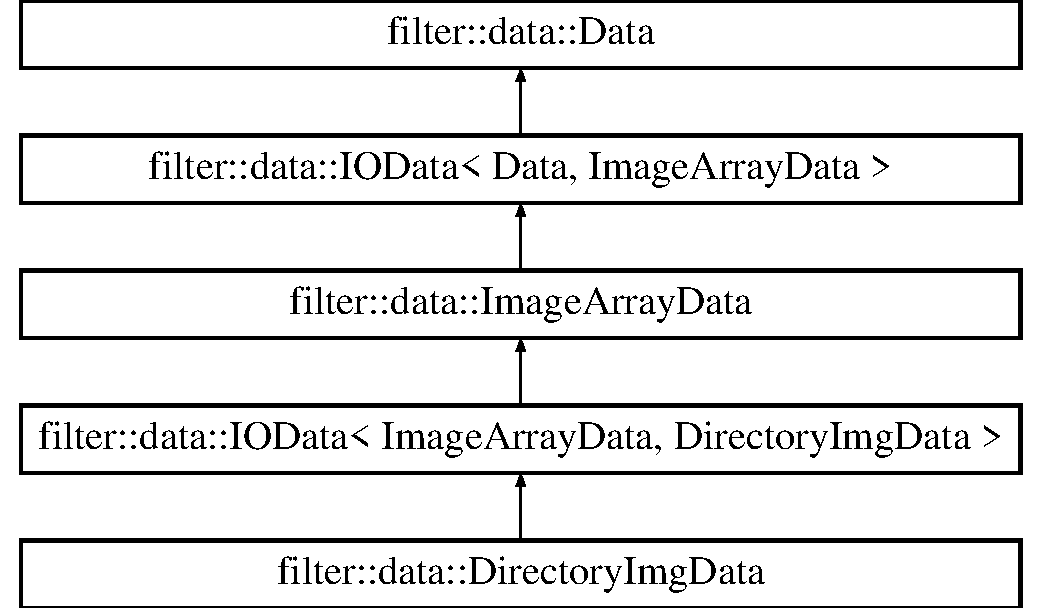
\includegraphics[height=5.000000cm]{d6/dd6/classfilter_1_1data_1_1_directory_img_data}
\end{center}
\end{figure}
\subsection*{Public Member Functions}
\begin{DoxyCompactItemize}
\item 
\hyperlink{classfilter_1_1data_1_1_directory_img_data_a7005a24110c2fe7de63a13bd4a082074}{Directory\+Img\+Data} (const std\+::string \&directory\+Path)
\item 
std\+::vector$<$ cv\+::\+Mat $>$ \& \hyperlink{classfilter_1_1data_1_1_directory_img_data_ae582abd2529b225ccdfe4d268333051f}{images} ()
\begin{DoxyCompactList}\small\item\em Get the container of the images\textquotesingle{} data. \end{DoxyCompactList}\item 
cv\+::\+Mat \hyperlink{classfilter_1_1data_1_1_directory_img_data_a2d2f7b78ebdc9adc1842447bec9f4fcb}{image} (int index)
\begin{DoxyCompactList}\small\item\em Get data of an image by its index in the container. \end{DoxyCompactList}\end{DoxyCompactItemize}
\subsection*{Private Attributes}
\begin{DoxyCompactItemize}
\item 
\mbox{\Hypertarget{classfilter_1_1data_1_1_directory_img_data_a21b17cc7584d78b5696d74e4227c2bc7}\label{classfilter_1_1data_1_1_directory_img_data_a21b17cc7584d78b5696d74e4227c2bc7}} 
std\+::string \hyperlink{classfilter_1_1data_1_1_directory_img_data_a21b17cc7584d78b5696d74e4227c2bc7}{\+\_\+directory\+Path}
\begin{DoxyCompactList}\small\item\em The path to the folder containing the images. \end{DoxyCompactList}\end{DoxyCompactItemize}
\subsection*{Additional Inherited Members}


\subsection{Constructor \& Destructor Documentation}
\mbox{\Hypertarget{classfilter_1_1data_1_1_directory_img_data_a7005a24110c2fe7de63a13bd4a082074}\label{classfilter_1_1data_1_1_directory_img_data_a7005a24110c2fe7de63a13bd4a082074}} 
\index{filter\+::data\+::\+Directory\+Img\+Data@{filter\+::data\+::\+Directory\+Img\+Data}!Directory\+Img\+Data@{Directory\+Img\+Data}}
\index{Directory\+Img\+Data@{Directory\+Img\+Data}!filter\+::data\+::\+Directory\+Img\+Data@{filter\+::data\+::\+Directory\+Img\+Data}}
\subsubsection{\texorpdfstring{Directory\+Img\+Data()}{DirectoryImgData()}}
{\footnotesize\ttfamily filter\+::data\+::\+Directory\+Img\+Data\+::\+Directory\+Img\+Data (\begin{DoxyParamCaption}\item[{const std\+::string \&}]{directory\+Path }\end{DoxyParamCaption})\hspace{0.3cm}{\ttfamily [inline]}}


\begin{DoxyParams}{Parameters}
{\em directory\+Path} & The path to where the images are located \\
\hline
\end{DoxyParams}


\subsection{Member Function Documentation}
\mbox{\Hypertarget{classfilter_1_1data_1_1_directory_img_data_a2d2f7b78ebdc9adc1842447bec9f4fcb}\label{classfilter_1_1data_1_1_directory_img_data_a2d2f7b78ebdc9adc1842447bec9f4fcb}} 
\index{filter\+::data\+::\+Directory\+Img\+Data@{filter\+::data\+::\+Directory\+Img\+Data}!image@{image}}
\index{image@{image}!filter\+::data\+::\+Directory\+Img\+Data@{filter\+::data\+::\+Directory\+Img\+Data}}
\subsubsection{\texorpdfstring{image()}{image()}}
{\footnotesize\ttfamily cv\+::\+Mat filter\+::data\+::\+Directory\+Img\+Data\+::image (\begin{DoxyParamCaption}\item[{int}]{index }\end{DoxyParamCaption})\hspace{0.3cm}{\ttfamily [inline]}}

\begin{DoxyReturn}{Returns}
Returns a cv\+::\+Mat object containing the image\textquotesingle{} data 
\end{DoxyReturn}
\mbox{\Hypertarget{classfilter_1_1data_1_1_directory_img_data_ae582abd2529b225ccdfe4d268333051f}\label{classfilter_1_1data_1_1_directory_img_data_ae582abd2529b225ccdfe4d268333051f}} 
\index{filter\+::data\+::\+Directory\+Img\+Data@{filter\+::data\+::\+Directory\+Img\+Data}!images@{images}}
\index{images@{images}!filter\+::data\+::\+Directory\+Img\+Data@{filter\+::data\+::\+Directory\+Img\+Data}}
\subsubsection{\texorpdfstring{images()}{images()}}
{\footnotesize\ttfamily std\+::vector$<$cv\+::\+Mat$>$\& filter\+::data\+::\+Directory\+Img\+Data\+::images (\begin{DoxyParamCaption}{ }\end{DoxyParamCaption})\hspace{0.3cm}{\ttfamily [inline]}}

\begin{DoxyReturn}{Returns}
Returns a reference to the std\+::vector$<$cv\+::\+Mat$>$ object containing the images\textquotesingle{} data 
\end{DoxyReturn}


The documentation for this class was generated from the following file\+:\begin{DoxyCompactItemize}
\item 
header/filter/data/Directory\+Img\+Data.\+h\end{DoxyCompactItemize}

\hypertarget{classdt_functor}{}\section{dt\+Functor Class Reference}
\label{classdt_functor}\index{dt\+Functor@{dt\+Functor}}
\subsection*{Classes}
\begin{DoxyCompactItemize}
\item 
struct \hyperlink{structdt_functor_1_1base}{base}
\item 
struct \hyperlink{structdt_functor_1_1wrapped}{wrapped}
\end{DoxyCompactItemize}
\subsection*{Public Member Functions}
\begin{DoxyCompactItemize}
\item 
\mbox{\Hypertarget{classdt_functor_a507910c3dcc0414497a17f6204d88671}\label{classdt_functor_a507910c3dcc0414497a17f6204d88671}} 
{\footnotesize template$<$typename... Args$>$ }\\{\bfseries dt\+Functor} (\hyperlink{classdt_functor}{dt\+Functor} \&a\+Func)
\item 
\mbox{\Hypertarget{classdt_functor_aacc40d2fed913a086e8649a5fe3bb24e}\label{classdt_functor_aacc40d2fed913a086e8649a5fe3bb24e}} 
{\footnotesize template$<$typename... Args$>$ }\\{\bfseries dt\+Functor} (const \hyperlink{classdt_functor}{dt\+Functor} \&a\+Func)
\item 
\mbox{\Hypertarget{classdt_functor_ab931dbe2c475bdfad4aee5df1d7d2f96}\label{classdt_functor_ab931dbe2c475bdfad4aee5df1d7d2f96}} 
{\footnotesize template$<$typename... Args$>$ }\\{\bfseries dt\+Functor} (std\+::function$<$ void(Args...)$>$ a\+Func)
\item 
\mbox{\Hypertarget{classdt_functor_a30c1a42395945cf200ac584a19e421d8}\label{classdt_functor_a30c1a42395945cf200ac584a19e421d8}} 
{\footnotesize template$<$typename... Args$>$ }\\\hyperlink{classdt_functor}{dt\+Functor} \& {\bfseries operator=} (std\+::function$<$ void(Args...)$>$ a\+Func)
\item 
\mbox{\Hypertarget{classdt_functor_ac8980a0e998d84ae700b0b56464cbf1c}\label{classdt_functor_ac8980a0e998d84ae700b0b56464cbf1c}} 
\hyperlink{classdt_functor}{dt\+Functor} \& {\bfseries operator=} (\hyperlink{classdt_functor}{dt\+Functor} \&dt\+Func)
\item 
\mbox{\Hypertarget{classdt_functor_a184225633c35c4be88afafca6661949b}\label{classdt_functor_a184225633c35c4be88afafca6661949b}} 
{\footnotesize template$<$class Obj , typename... Args$>$ }\\void {\bfseries operator()} (Obj obj, Args... args) const
\end{DoxyCompactItemize}
\subsection*{Private Attributes}
\begin{DoxyCompactItemize}
\item 
\mbox{\Hypertarget{classdt_functor_a48539a2d735d52557d89c00f3623bfb7}\label{classdt_functor_a48539a2d735d52557d89c00f3623bfb7}} 
std\+::unique\+\_\+ptr$<$ \hyperlink{structdt_functor_1_1base}{base} $>$ {\bfseries p\+\_\+base}
\end{DoxyCompactItemize}


The documentation for this class was generated from the following file\+:\begin{DoxyCompactItemize}
\item 
header/filter/tools/functor.\+hpp\end{DoxyCompactItemize}

\hypertarget{classfilter_1_1algos_1_1_equalize}{}\section{filter\+:\+:algos\+:\+:Equalize Class Reference}
\label{classfilter_1_1algos_1_1_equalize}\index{filter\+::algos\+::\+Equalize@{filter\+::algos\+::\+Equalize}}


The \hyperlink{classfilter_1_1algos_1_1_equalize}{Equalize} filter will equalize the image histogram resulting of the input image analysis. It will improve the contrast of the image.  




{\ttfamily \#include $<$Equalize.\+h$>$}

Inheritance diagram for filter\+:\+:algos\+:\+:Equalize\+:\begin{figure}[H]
\begin{center}
\leavevmode
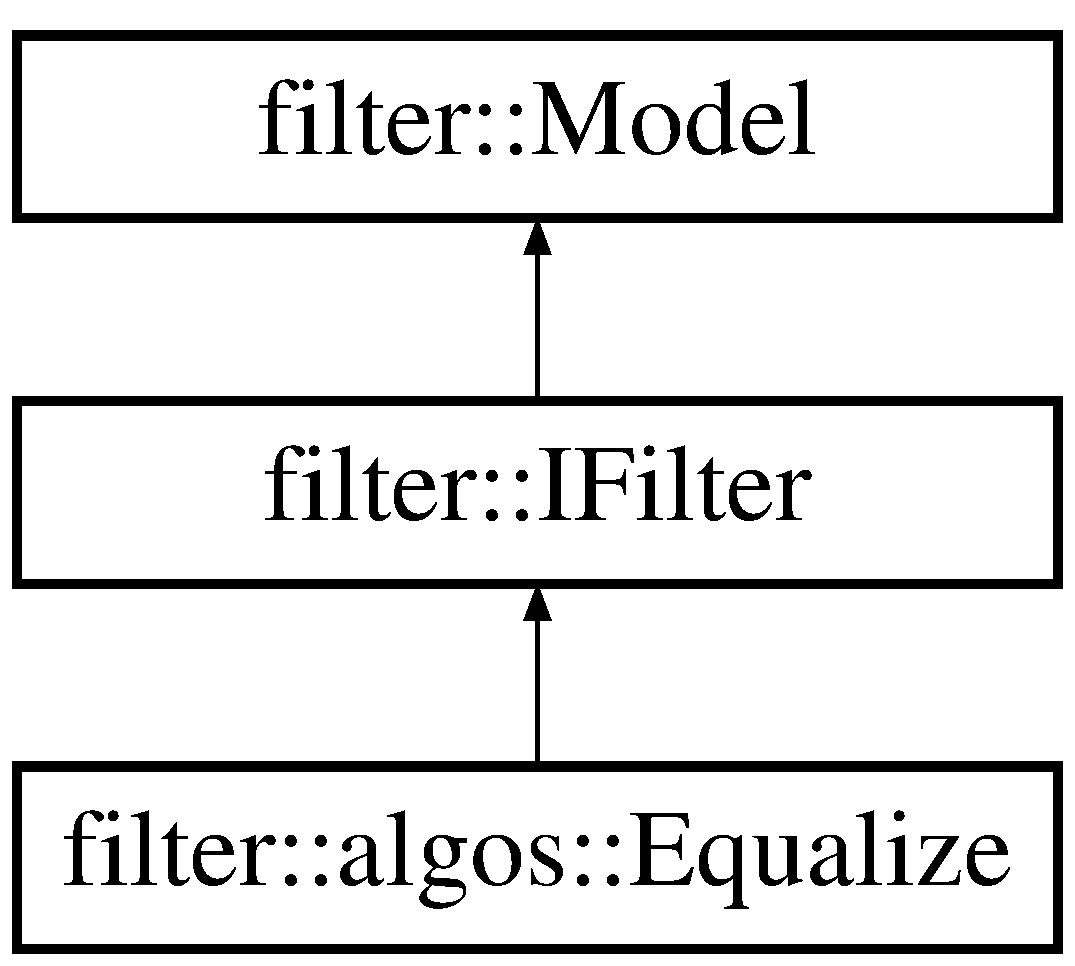
\includegraphics[height=3.000000cm]{d9/ddf/classfilter_1_1algos_1_1_equalize}
\end{center}
\end{figure}
\subsection*{Public Types}
\begin{DoxyCompactItemize}
\item 
\mbox{\Hypertarget{classfilter_1_1algos_1_1_equalize_a0c7b19c96f65d70f4d96cd4eb24f4a70}\label{classfilter_1_1algos_1_1_equalize_a0c7b19c96f65d70f4d96cd4eb24f4a70}} 
typedef \hyperlink{class_proxy_functor}{Proxy\+Functor}$<$ \hyperlink{classfilter_1_1algos_1_1_equalize}{Equalize} $>$ {\bfseries \+\_\+proxy\+Functor}
\item 
\mbox{\Hypertarget{classfilter_1_1algos_1_1_equalize_a571bedd9a3a876726a8f5096ac1722a6}\label{classfilter_1_1algos_1_1_equalize_a571bedd9a3a876726a8f5096ac1722a6}} 
typedef \hyperlink{classfilter_1_1algos_1_1_equalize}{Equalize} {\bfseries mytype}
\item 
\mbox{\Hypertarget{classfilter_1_1algos_1_1_equalize_a4680b6a6b15ed69ad53d47bae4ca5153}\label{classfilter_1_1algos_1_1_equalize_a4680b6a6b15ed69ad53d47bae4ca5153}} 
typedef char {\bfseries vartype\+\_\+\+\_\+unused}
\end{DoxyCompactItemize}
\subsection*{Public Member Functions}
\begin{DoxyCompactItemize}
\item 
\mbox{\Hypertarget{classfilter_1_1algos_1_1_equalize_a94bb1623cf50c194b662fe9710830bf1}\label{classfilter_1_1algos_1_1_equalize_a94bb1623cf50c194b662fe9710830bf1}} 
void {\bfseries set\+\_\+unused\+\_\+from\+\_\+json} (boost\+::property\+\_\+tree\+::ptree \&json\+Class)
\item 
\mbox{\Hypertarget{classfilter_1_1algos_1_1_equalize_a189140d796929dbd825cf812e49671f8}\label{classfilter_1_1algos_1_1_equalize_a189140d796929dbd825cf812e49671f8}} 
void {\bfseries set\+\_\+unused} (vartype\+\_\+\+\_\+unused \&\+\_\+\+\_\+unused)
\item 
\mbox{\Hypertarget{classfilter_1_1algos_1_1_equalize_abae70dc2f14663a0a993804fcacca148}\label{classfilter_1_1algos_1_1_equalize_abae70dc2f14663a0a993804fcacca148}} 
vartype\+\_\+\+\_\+unused {\bfseries get\+\_\+unused} ()
\item 
\mbox{\Hypertarget{classfilter_1_1algos_1_1_equalize_a4e79d84feb301fad3053dca19dcbeca6}\label{classfilter_1_1algos_1_1_equalize_a4e79d84feb301fad3053dca19dcbeca6}} 
void {\bfseries copy\+\_\+unused} (\hyperlink{classfilter_1_1algos_1_1_equalize}{mytype} $\ast$instance)
\item 
\mbox{\Hypertarget{classfilter_1_1algos_1_1_equalize_a3673dfdd4f89f0999ff868c908cec097}\label{classfilter_1_1algos_1_1_equalize_a3673dfdd4f89f0999ff868c908cec097}} 
Hipe\+Status {\bfseries process} () override
\end{DoxyCompactItemize}
\subsection*{Public Attributes}
\begin{DoxyCompactItemize}
\item 
\mbox{\Hypertarget{classfilter_1_1algos_1_1_equalize_a203e0b132be3ed0261159f6e272b4509}\label{classfilter_1_1algos_1_1_equalize_a203e0b132be3ed0261159f6e272b4509}} 
char {\bfseries unused}
\end{DoxyCompactItemize}
\subsection*{Private Member Functions}
\begin{DoxyCompactItemize}
\item 
\mbox{\Hypertarget{classfilter_1_1algos_1_1_equalize_a95d03a7b04858455c3a3bd851669afaf}\label{classfilter_1_1algos_1_1_equalize_a95d03a7b04858455c3a3bd851669afaf}} 
virtual \hyperlink{classfilter_1_1data_1_1_connex_data_base}{data\+::\+Connex\+Data\+Base} \& {\bfseries get\+Connector} ()
\end{DoxyCompactItemize}
\subsection*{Private Attributes}
\begin{DoxyCompactItemize}
\item 
\mbox{\Hypertarget{classfilter_1_1algos_1_1_equalize_a32bb5b9588251a938a086fd8d08e820c}\label{classfilter_1_1algos_1_1_equalize_a32bb5b9588251a938a086fd8d08e820c}} 
\hyperlink{classfilter_1_1data_1_1_connex_data}{data\+::\+Connex\+Data}$<$ \hyperlink{classfilter_1_1data_1_1_image_data}{data\+::\+Image\+Data}, \hyperlink{classfilter_1_1data_1_1_image_data}{data\+::\+Image\+Data} $>$ {\bfseries \+\_\+connex\+Data}
\end{DoxyCompactItemize}
\subsection*{Additional Inherited Members}


\subsection{Detailed Description}
\begin{DoxySeeAlso}{See also}
cv\+::equalize\+Hist() 
\end{DoxySeeAlso}


The documentation for this class was generated from the following file\+:\begin{DoxyCompactItemize}
\item 
header/filter/\+Algos/Equalize.\+h\end{DoxyCompactItemize}

\hypertarget{classfilter_1_1algos_1_1_equalize_adaptive}{}\section{filter\+:\+:algos\+:\+:Equalize\+Adaptive Class Reference}
\label{classfilter_1_1algos_1_1_equalize_adaptive}\index{filter\+::algos\+::\+Equalize\+Adaptive@{filter\+::algos\+::\+Equalize\+Adaptive}}


The \hyperlink{classfilter_1_1algos_1_1_equalize_adaptive}{Equalize\+Adaptive} filter will equalize the image histogram resulting of the input image analysis. It will improve the contrast of the image.  




{\ttfamily \#include $<$Equalize\+Adaptive.\+h$>$}

Inheritance diagram for filter\+:\+:algos\+:\+:Equalize\+Adaptive\+:\begin{figure}[H]
\begin{center}
\leavevmode
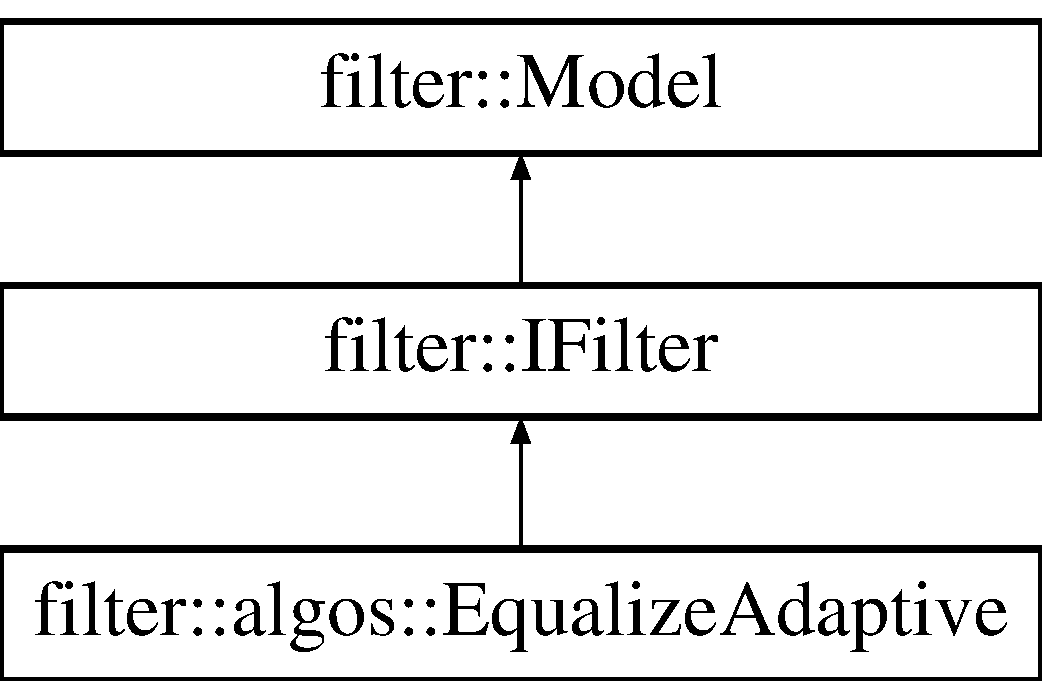
\includegraphics[height=3.000000cm]{d1/de5/classfilter_1_1algos_1_1_equalize_adaptive}
\end{center}
\end{figure}
\subsection*{Public Types}
\begin{DoxyCompactItemize}
\item 
\mbox{\Hypertarget{classfilter_1_1algos_1_1_equalize_adaptive_a481933032e94867c528a90f7f11249e8}\label{classfilter_1_1algos_1_1_equalize_adaptive_a481933032e94867c528a90f7f11249e8}} 
typedef \hyperlink{class_proxy_functor}{Proxy\+Functor}$<$ \hyperlink{classfilter_1_1algos_1_1_equalize_adaptive}{Equalize\+Adaptive} $>$ {\bfseries \+\_\+proxy\+Functor}
\item 
\mbox{\Hypertarget{classfilter_1_1algos_1_1_equalize_adaptive_a4bb3ef65b29a2541a1966d0c7f6fcafb}\label{classfilter_1_1algos_1_1_equalize_adaptive_a4bb3ef65b29a2541a1966d0c7f6fcafb}} 
typedef \hyperlink{classfilter_1_1algos_1_1_equalize_adaptive}{Equalize\+Adaptive} {\bfseries mytype}
\item 
\mbox{\Hypertarget{classfilter_1_1algos_1_1_equalize_adaptive_aec362799ac1e93a7e4242ef95e4f38a2}\label{classfilter_1_1algos_1_1_equalize_adaptive_aec362799ac1e93a7e4242ef95e4f38a2}} 
typedef double {\bfseries vartype\+\_\+\+\_\+clip}
\item 
\mbox{\Hypertarget{classfilter_1_1algos_1_1_equalize_adaptive_af6d0553efaddee0a597bbb7409a52b1a}\label{classfilter_1_1algos_1_1_equalize_adaptive_af6d0553efaddee0a597bbb7409a52b1a}} 
typedef int {\bfseries vartype\+\_\+\+\_\+kernel}
\end{DoxyCompactItemize}
\subsection*{Public Member Functions}
\begin{DoxyCompactItemize}
\item 
\mbox{\Hypertarget{classfilter_1_1algos_1_1_equalize_adaptive_aa17780085e82d6e33f77767852db82cb}\label{classfilter_1_1algos_1_1_equalize_adaptive_aa17780085e82d6e33f77767852db82cb}} 
void {\bfseries set\+\_\+clip\+\_\+from\+\_\+json} (boost\+::property\+\_\+tree\+::ptree \&json\+Class)
\item 
\mbox{\Hypertarget{classfilter_1_1algos_1_1_equalize_adaptive_ab0b8097aa4a0340f00ae24a074934a97}\label{classfilter_1_1algos_1_1_equalize_adaptive_ab0b8097aa4a0340f00ae24a074934a97}} 
void {\bfseries set\+\_\+clip} (vartype\+\_\+\+\_\+clip \&\+\_\+\+\_\+clip)
\item 
\mbox{\Hypertarget{classfilter_1_1algos_1_1_equalize_adaptive_a0f29eb8ccdb8888e43c6e90777edb6fb}\label{classfilter_1_1algos_1_1_equalize_adaptive_a0f29eb8ccdb8888e43c6e90777edb6fb}} 
vartype\+\_\+\+\_\+clip {\bfseries get\+\_\+clip} ()
\item 
\mbox{\Hypertarget{classfilter_1_1algos_1_1_equalize_adaptive_af379a2bfdb1cb898407a3cf51da57208}\label{classfilter_1_1algos_1_1_equalize_adaptive_af379a2bfdb1cb898407a3cf51da57208}} 
void {\bfseries copy\+\_\+clip} (\hyperlink{classfilter_1_1algos_1_1_equalize_adaptive}{mytype} $\ast$instance)
\item 
\mbox{\Hypertarget{classfilter_1_1algos_1_1_equalize_adaptive_a84a7322947293f27cd4cdcef660a8a8f}\label{classfilter_1_1algos_1_1_equalize_adaptive_a84a7322947293f27cd4cdcef660a8a8f}} 
void {\bfseries set\+\_\+kernel\+\_\+from\+\_\+json} (boost\+::property\+\_\+tree\+::ptree \&json\+Class)
\item 
\mbox{\Hypertarget{classfilter_1_1algos_1_1_equalize_adaptive_aaa3bf471bf037a580903da9311169355}\label{classfilter_1_1algos_1_1_equalize_adaptive_aaa3bf471bf037a580903da9311169355}} 
void {\bfseries set\+\_\+kernel} (vartype\+\_\+\+\_\+kernel \&\+\_\+\+\_\+kernel)
\item 
\mbox{\Hypertarget{classfilter_1_1algos_1_1_equalize_adaptive_a5f0e936b76dd8548d6835aa26c141709}\label{classfilter_1_1algos_1_1_equalize_adaptive_a5f0e936b76dd8548d6835aa26c141709}} 
vartype\+\_\+\+\_\+kernel {\bfseries get\+\_\+kernel} ()
\item 
\mbox{\Hypertarget{classfilter_1_1algos_1_1_equalize_adaptive_af84e3c9a81beeb3aa74357b0450d9289}\label{classfilter_1_1algos_1_1_equalize_adaptive_af84e3c9a81beeb3aa74357b0450d9289}} 
void {\bfseries copy\+\_\+kernel} (\hyperlink{classfilter_1_1algos_1_1_equalize_adaptive}{mytype} $\ast$instance)
\item 
\mbox{\Hypertarget{classfilter_1_1algos_1_1_equalize_adaptive_a03d8e13b8a827898f7cef8b171a701a5}\label{classfilter_1_1algos_1_1_equalize_adaptive_a03d8e13b8a827898f7cef8b171a701a5}} 
Hipe\+Status {\bfseries process} () override
\end{DoxyCompactItemize}
\subsection*{Public Attributes}
\begin{DoxyCompactItemize}
\item 
double \hyperlink{classfilter_1_1algos_1_1_equalize_adaptive_a46afdee63800444f373e4eae9fc9cc3a}{clip}
\item 
int \hyperlink{classfilter_1_1algos_1_1_equalize_adaptive_ae190d8c8f0cb57cd1a2fb2fc778c963a}{kernel}
\end{DoxyCompactItemize}
\subsection*{Private Member Functions}
\begin{DoxyCompactItemize}
\item 
\mbox{\Hypertarget{classfilter_1_1algos_1_1_equalize_adaptive_ab31327e7baf064f4287d99e013a0e6e4}\label{classfilter_1_1algos_1_1_equalize_adaptive_ab31327e7baf064f4287d99e013a0e6e4}} 
virtual \hyperlink{classfilter_1_1data_1_1_connex_data_base}{data\+::\+Connex\+Data\+Base} \& {\bfseries get\+Connector} ()
\end{DoxyCompactItemize}
\subsection*{Private Attributes}
\begin{DoxyCompactItemize}
\item 
\mbox{\Hypertarget{classfilter_1_1algos_1_1_equalize_adaptive_a4209d59f9412e9ef1d562a66f10f1e93}\label{classfilter_1_1algos_1_1_equalize_adaptive_a4209d59f9412e9ef1d562a66f10f1e93}} 
\hyperlink{classfilter_1_1data_1_1_connex_data}{data\+::\+Connex\+Data}$<$ \hyperlink{classfilter_1_1data_1_1_image_data}{data\+::\+Image\+Data}, \hyperlink{classfilter_1_1data_1_1_image_data}{data\+::\+Image\+Data} $>$ {\bfseries \+\_\+connex\+Data}
\end{DoxyCompactItemize}
\subsection*{Additional Inherited Members}


\subsection{Detailed Description}
Instead of doing it on the whole image like the \hyperlink{classfilter_1_1algos_1_1_equalize}{Equalize} filter, it will subdivide it in multiple parts and work on them separately. \begin{DoxySeeAlso}{See also}
cv\+::\+C\+L\+A\+HE 
\end{DoxySeeAlso}


\subsection{Member Data Documentation}
\mbox{\Hypertarget{classfilter_1_1algos_1_1_equalize_adaptive_a46afdee63800444f373e4eae9fc9cc3a}\label{classfilter_1_1algos_1_1_equalize_adaptive_a46afdee63800444f373e4eae9fc9cc3a}} 
\index{filter\+::algos\+::\+Equalize\+Adaptive@{filter\+::algos\+::\+Equalize\+Adaptive}!clip@{clip}}
\index{clip@{clip}!filter\+::algos\+::\+Equalize\+Adaptive@{filter\+::algos\+::\+Equalize\+Adaptive}}
\subsubsection{\texorpdfstring{clip}{clip}}
{\footnotesize\ttfamily filter\+::algos\+::\+Equalize\+Adaptive\+::clip}

The clipping (contrast) limit. The maximum contranst a bin can have. If it is superior it will be clipped and distribued equally to the surrounding ones. \mbox{\Hypertarget{classfilter_1_1algos_1_1_equalize_adaptive_ae190d8c8f0cb57cd1a2fb2fc778c963a}\label{classfilter_1_1algos_1_1_equalize_adaptive_ae190d8c8f0cb57cd1a2fb2fc778c963a}} 
\index{filter\+::algos\+::\+Equalize\+Adaptive@{filter\+::algos\+::\+Equalize\+Adaptive}!kernel@{kernel}}
\index{kernel@{kernel}!filter\+::algos\+::\+Equalize\+Adaptive@{filter\+::algos\+::\+Equalize\+Adaptive}}
\subsubsection{\texorpdfstring{kernel}{kernel}}
{\footnotesize\ttfamily filter\+::algos\+::\+Equalize\+Adaptive\+::kernel}

The size each subdivision should have. 

The documentation for this class was generated from the following file\+:\begin{DoxyCompactItemize}
\item 
header/filter/\+Algos/Equalize\+Adaptive.\+h\end{DoxyCompactItemize}

\hypertarget{classfilter_1_1algos_1_1_erode}{}\section{filter\+:\+:algos\+:\+:Erode Class Reference}
\label{classfilter_1_1algos_1_1_erode}\index{filter\+::algos\+::\+Erode@{filter\+::algos\+::\+Erode}}
Inheritance diagram for filter\+:\+:algos\+:\+:Erode\+:\begin{figure}[H]
\begin{center}
\leavevmode
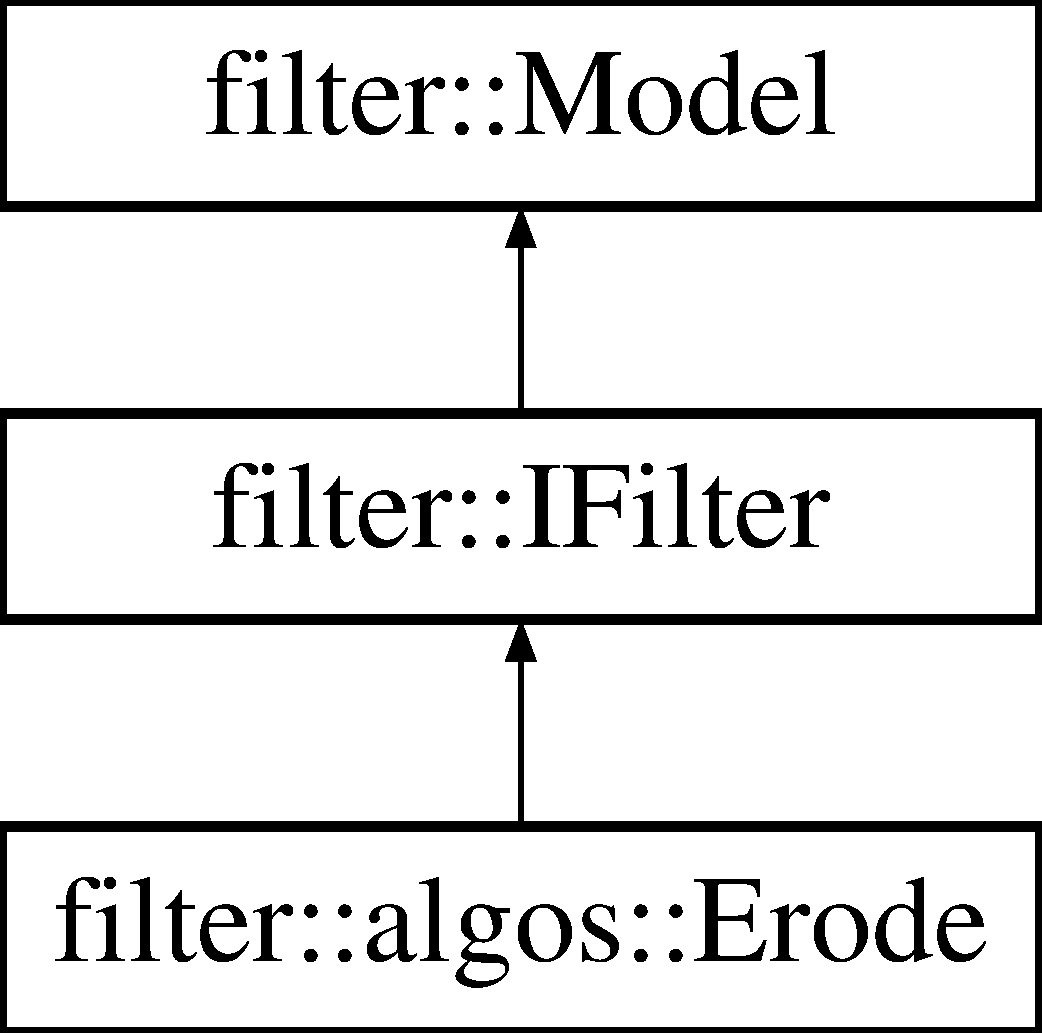
\includegraphics[height=3.000000cm]{d5/dc3/classfilter_1_1algos_1_1_erode}
\end{center}
\end{figure}
\subsection*{Public Types}
\begin{DoxyCompactItemize}
\item 
\mbox{\Hypertarget{classfilter_1_1algos_1_1_erode_a0dae564b3f9d318acb9ecf5b967dc295}\label{classfilter_1_1algos_1_1_erode_a0dae564b3f9d318acb9ecf5b967dc295}} 
typedef \hyperlink{class_proxy_functor}{Proxy\+Functor}$<$ \hyperlink{classfilter_1_1algos_1_1_erode}{Erode} $>$ {\bfseries \+\_\+proxy\+Functor}
\item 
\mbox{\Hypertarget{classfilter_1_1algos_1_1_erode_a315c4dfcad46e0086526a60c892c3d74}\label{classfilter_1_1algos_1_1_erode_a315c4dfcad46e0086526a60c892c3d74}} 
typedef \hyperlink{classfilter_1_1algos_1_1_erode}{Erode} {\bfseries mytype}
\item 
\mbox{\Hypertarget{classfilter_1_1algos_1_1_erode_a24c830675119cb4673b3adbd47d481fc}\label{classfilter_1_1algos_1_1_erode_a24c830675119cb4673b3adbd47d481fc}} 
typedef int {\bfseries vartype\+\_\+\+\_\+iterations}
\item 
\mbox{\Hypertarget{classfilter_1_1algos_1_1_erode_a63e06d047f04a11eaca2419ae28418ac}\label{classfilter_1_1algos_1_1_erode_a63e06d047f04a11eaca2419ae28418ac}} 
typedef std\+::string {\bfseries vartype\+\_\+\+\_\+morph\+Type}
\item 
\mbox{\Hypertarget{classfilter_1_1algos_1_1_erode_aba2adb9ce2397fc1fae3b0fb5c664f81}\label{classfilter_1_1algos_1_1_erode_aba2adb9ce2397fc1fae3b0fb5c664f81}} 
typedef std\+::string {\bfseries vartype\+\_\+\+\_\+morph\+Shape}
\item 
\mbox{\Hypertarget{classfilter_1_1algos_1_1_erode_a402f6f07baab72f5495274d8badf2089}\label{classfilter_1_1algos_1_1_erode_a402f6f07baab72f5495274d8badf2089}} 
typedef int {\bfseries vartype\+\_\+\+\_\+kernel\+SizeX}
\item 
\mbox{\Hypertarget{classfilter_1_1algos_1_1_erode_a7848d2eb18420a14fe5ee09242c8c9a5}\label{classfilter_1_1algos_1_1_erode_a7848d2eb18420a14fe5ee09242c8c9a5}} 
typedef int {\bfseries vartype\+\_\+\+\_\+kernel\+SizeY}
\item 
\mbox{\Hypertarget{classfilter_1_1algos_1_1_erode_a2fce3a51dd2b228a242f3c6e2dbc2a0b}\label{classfilter_1_1algos_1_1_erode_a2fce3a51dd2b228a242f3c6e2dbc2a0b}} 
typedef int {\bfseries vartype\+\_\+\+\_\+anchorX}
\item 
\mbox{\Hypertarget{classfilter_1_1algos_1_1_erode_a3d52f0f9da087b31ed4e8fd801b68f7e}\label{classfilter_1_1algos_1_1_erode_a3d52f0f9da087b31ed4e8fd801b68f7e}} 
typedef int {\bfseries vartype\+\_\+\+\_\+anchorY}
\end{DoxyCompactItemize}
\subsection*{Public Member Functions}
\begin{DoxyCompactItemize}
\item 
\mbox{\Hypertarget{classfilter_1_1algos_1_1_erode_adfe5cb49788dbdbb0bf58813ba103e07}\label{classfilter_1_1algos_1_1_erode_adfe5cb49788dbdbb0bf58813ba103e07}} 
void {\bfseries set\+\_\+iterations\+\_\+from\+\_\+json} (boost\+::property\+\_\+tree\+::ptree \&json\+Class)
\item 
\mbox{\Hypertarget{classfilter_1_1algos_1_1_erode_a8af40724658d8f4b2f3be7e7226b5e27}\label{classfilter_1_1algos_1_1_erode_a8af40724658d8f4b2f3be7e7226b5e27}} 
void {\bfseries set\+\_\+iterations} (vartype\+\_\+\+\_\+iterations \&\+\_\+\+\_\+iterations)
\item 
\mbox{\Hypertarget{classfilter_1_1algos_1_1_erode_a29deab7218652d4e48e2fda4c7cb093e}\label{classfilter_1_1algos_1_1_erode_a29deab7218652d4e48e2fda4c7cb093e}} 
vartype\+\_\+\+\_\+iterations {\bfseries get\+\_\+iterations} ()
\item 
\mbox{\Hypertarget{classfilter_1_1algos_1_1_erode_a92d4693fdb5ee9e1afbfa26fc5fe4b14}\label{classfilter_1_1algos_1_1_erode_a92d4693fdb5ee9e1afbfa26fc5fe4b14}} 
void {\bfseries copy\+\_\+iterations} (\hyperlink{classfilter_1_1algos_1_1_erode}{mytype} $\ast$instance)
\item 
\mbox{\Hypertarget{classfilter_1_1algos_1_1_erode_aa59744735acf12547a9b254beccfaadc}\label{classfilter_1_1algos_1_1_erode_aa59744735acf12547a9b254beccfaadc}} 
void {\bfseries set\+\_\+morph\+Type\+\_\+from\+\_\+json} (boost\+::property\+\_\+tree\+::ptree \&json\+Class)
\item 
\mbox{\Hypertarget{classfilter_1_1algos_1_1_erode_a5c76c50fa86a77514353d5e2e9a7ae35}\label{classfilter_1_1algos_1_1_erode_a5c76c50fa86a77514353d5e2e9a7ae35}} 
void {\bfseries set\+\_\+morph\+Type} (vartype\+\_\+\+\_\+morph\+Type \&\+\_\+\+\_\+morph\+Type)
\item 
\mbox{\Hypertarget{classfilter_1_1algos_1_1_erode_a9403bf4be3b8271c319cb302de5a326e}\label{classfilter_1_1algos_1_1_erode_a9403bf4be3b8271c319cb302de5a326e}} 
vartype\+\_\+\+\_\+morph\+Type {\bfseries get\+\_\+morph\+Type} ()
\item 
\mbox{\Hypertarget{classfilter_1_1algos_1_1_erode_a085dafc4c60d30dd3ac81e69ad28e2b0}\label{classfilter_1_1algos_1_1_erode_a085dafc4c60d30dd3ac81e69ad28e2b0}} 
void {\bfseries copy\+\_\+morph\+Type} (\hyperlink{classfilter_1_1algos_1_1_erode}{mytype} $\ast$instance)
\item 
\mbox{\Hypertarget{classfilter_1_1algos_1_1_erode_ae62c10b0d7de4db15353c3d31ec23e85}\label{classfilter_1_1algos_1_1_erode_ae62c10b0d7de4db15353c3d31ec23e85}} 
void {\bfseries set\+\_\+morph\+Shape\+\_\+from\+\_\+json} (boost\+::property\+\_\+tree\+::ptree \&json\+Class)
\item 
\mbox{\Hypertarget{classfilter_1_1algos_1_1_erode_aaf5fefca25e902b080f08a90e6430322}\label{classfilter_1_1algos_1_1_erode_aaf5fefca25e902b080f08a90e6430322}} 
void {\bfseries set\+\_\+morph\+Shape} (vartype\+\_\+\+\_\+morph\+Shape \&\+\_\+\+\_\+morph\+Shape)
\item 
\mbox{\Hypertarget{classfilter_1_1algos_1_1_erode_a39687897a97d74f63902f362869898fd}\label{classfilter_1_1algos_1_1_erode_a39687897a97d74f63902f362869898fd}} 
vartype\+\_\+\+\_\+morph\+Shape {\bfseries get\+\_\+morph\+Shape} ()
\item 
\mbox{\Hypertarget{classfilter_1_1algos_1_1_erode_ab7fda02d0119f71b3ce87a1239df39a2}\label{classfilter_1_1algos_1_1_erode_ab7fda02d0119f71b3ce87a1239df39a2}} 
void {\bfseries copy\+\_\+morph\+Shape} (\hyperlink{classfilter_1_1algos_1_1_erode}{mytype} $\ast$instance)
\item 
\mbox{\Hypertarget{classfilter_1_1algos_1_1_erode_ab0a222589d1e566ac24c26fd36e7f2d7}\label{classfilter_1_1algos_1_1_erode_ab0a222589d1e566ac24c26fd36e7f2d7}} 
void {\bfseries set\+\_\+kernel\+Size\+X\+\_\+from\+\_\+json} (boost\+::property\+\_\+tree\+::ptree \&json\+Class)
\item 
\mbox{\Hypertarget{classfilter_1_1algos_1_1_erode_aa2171026ed4aaa7f2d0cba470cb9b242}\label{classfilter_1_1algos_1_1_erode_aa2171026ed4aaa7f2d0cba470cb9b242}} 
void {\bfseries set\+\_\+kernel\+SizeX} (vartype\+\_\+\+\_\+kernel\+SizeX \&\+\_\+\+\_\+kernel\+SizeX)
\item 
\mbox{\Hypertarget{classfilter_1_1algos_1_1_erode_a8b6d26b1c233380cc06b9076fd6f7cb8}\label{classfilter_1_1algos_1_1_erode_a8b6d26b1c233380cc06b9076fd6f7cb8}} 
vartype\+\_\+\+\_\+kernel\+SizeX {\bfseries get\+\_\+kernel\+SizeX} ()
\item 
\mbox{\Hypertarget{classfilter_1_1algos_1_1_erode_a153940be3d6f373b16c1a1c795ccc865}\label{classfilter_1_1algos_1_1_erode_a153940be3d6f373b16c1a1c795ccc865}} 
void {\bfseries copy\+\_\+kernel\+SizeX} (\hyperlink{classfilter_1_1algos_1_1_erode}{mytype} $\ast$instance)
\item 
\mbox{\Hypertarget{classfilter_1_1algos_1_1_erode_a08b82a5bd31318de2303e30749de6a4e}\label{classfilter_1_1algos_1_1_erode_a08b82a5bd31318de2303e30749de6a4e}} 
void {\bfseries set\+\_\+kernel\+Size\+Y\+\_\+from\+\_\+json} (boost\+::property\+\_\+tree\+::ptree \&json\+Class)
\item 
\mbox{\Hypertarget{classfilter_1_1algos_1_1_erode_a4933bc5cc3c5aa822ee0efc461df09bd}\label{classfilter_1_1algos_1_1_erode_a4933bc5cc3c5aa822ee0efc461df09bd}} 
void {\bfseries set\+\_\+kernel\+SizeY} (vartype\+\_\+\+\_\+kernel\+SizeY \&\+\_\+\+\_\+kernel\+SizeY)
\item 
\mbox{\Hypertarget{classfilter_1_1algos_1_1_erode_a299149c462c4059716657a5f6775c269}\label{classfilter_1_1algos_1_1_erode_a299149c462c4059716657a5f6775c269}} 
vartype\+\_\+\+\_\+kernel\+SizeY {\bfseries get\+\_\+kernel\+SizeY} ()
\item 
\mbox{\Hypertarget{classfilter_1_1algos_1_1_erode_aa6cf1c5ba5ab7900de746ef94457c28f}\label{classfilter_1_1algos_1_1_erode_aa6cf1c5ba5ab7900de746ef94457c28f}} 
void {\bfseries copy\+\_\+kernel\+SizeY} (\hyperlink{classfilter_1_1algos_1_1_erode}{mytype} $\ast$instance)
\item 
\mbox{\Hypertarget{classfilter_1_1algos_1_1_erode_aaeb950e83cd0141c154b8f553c34b387}\label{classfilter_1_1algos_1_1_erode_aaeb950e83cd0141c154b8f553c34b387}} 
void {\bfseries set\+\_\+anchor\+X\+\_\+from\+\_\+json} (boost\+::property\+\_\+tree\+::ptree \&json\+Class)
\item 
\mbox{\Hypertarget{classfilter_1_1algos_1_1_erode_aafe71bf03f3f577ef490b1d1327f4ec9}\label{classfilter_1_1algos_1_1_erode_aafe71bf03f3f577ef490b1d1327f4ec9}} 
void {\bfseries set\+\_\+anchorX} (vartype\+\_\+\+\_\+anchorX \&\+\_\+\+\_\+anchorX)
\item 
\mbox{\Hypertarget{classfilter_1_1algos_1_1_erode_a295542f1145a19e764f4722eb72cbc6c}\label{classfilter_1_1algos_1_1_erode_a295542f1145a19e764f4722eb72cbc6c}} 
vartype\+\_\+\+\_\+anchorX {\bfseries get\+\_\+anchorX} ()
\item 
\mbox{\Hypertarget{classfilter_1_1algos_1_1_erode_a8c24363a78ff22e5bbe6105ac10426ac}\label{classfilter_1_1algos_1_1_erode_a8c24363a78ff22e5bbe6105ac10426ac}} 
void {\bfseries copy\+\_\+anchorX} (\hyperlink{classfilter_1_1algos_1_1_erode}{mytype} $\ast$instance)
\item 
\mbox{\Hypertarget{classfilter_1_1algos_1_1_erode_aae017ac91c239c51569f7be55c6eff83}\label{classfilter_1_1algos_1_1_erode_aae017ac91c239c51569f7be55c6eff83}} 
void {\bfseries set\+\_\+anchor\+Y\+\_\+from\+\_\+json} (boost\+::property\+\_\+tree\+::ptree \&json\+Class)
\item 
\mbox{\Hypertarget{classfilter_1_1algos_1_1_erode_a0ff67e691820bdf696f264836c806ca1}\label{classfilter_1_1algos_1_1_erode_a0ff67e691820bdf696f264836c806ca1}} 
void {\bfseries set\+\_\+anchorY} (vartype\+\_\+\+\_\+anchorY \&\+\_\+\+\_\+anchorY)
\item 
\mbox{\Hypertarget{classfilter_1_1algos_1_1_erode_a42a3c13177f3756c07291c1bae19f8a4}\label{classfilter_1_1algos_1_1_erode_a42a3c13177f3756c07291c1bae19f8a4}} 
vartype\+\_\+\+\_\+anchorY {\bfseries get\+\_\+anchorY} ()
\item 
\mbox{\Hypertarget{classfilter_1_1algos_1_1_erode_a3650b5064832039e85049883df7ac4a9}\label{classfilter_1_1algos_1_1_erode_a3650b5064832039e85049883df7ac4a9}} 
void {\bfseries copy\+\_\+anchorY} (\hyperlink{classfilter_1_1algos_1_1_erode}{mytype} $\ast$instance)
\item 
\mbox{\Hypertarget{classfilter_1_1algos_1_1_erode_a3307e2b455b2dd757bb8afa08e1c5df3}\label{classfilter_1_1algos_1_1_erode_a3307e2b455b2dd757bb8afa08e1c5df3}} 
Hipe\+Status {\bfseries process} () override
\end{DoxyCompactItemize}
\subsection*{Public Attributes}
\begin{DoxyCompactItemize}
\item 
\mbox{\Hypertarget{classfilter_1_1algos_1_1_erode_add7d75df990a81e384dc121aee66a1db}\label{classfilter_1_1algos_1_1_erode_add7d75df990a81e384dc121aee66a1db}} 
int {\bfseries iterations}
\item 
\mbox{\Hypertarget{classfilter_1_1algos_1_1_erode_a4ce0ba3028d392dc896150f5ae9c52c1}\label{classfilter_1_1algos_1_1_erode_a4ce0ba3028d392dc896150f5ae9c52c1}} 
std\+::string {\bfseries morph\+Type}
\item 
\mbox{\Hypertarget{classfilter_1_1algos_1_1_erode_aa227fda26f1a3f22565503ac582ca64f}\label{classfilter_1_1algos_1_1_erode_aa227fda26f1a3f22565503ac582ca64f}} 
std\+::string {\bfseries morph\+Shape}
\item 
\mbox{\Hypertarget{classfilter_1_1algos_1_1_erode_a800d0e2bc5b0dd558c03b9439e001afa}\label{classfilter_1_1algos_1_1_erode_a800d0e2bc5b0dd558c03b9439e001afa}} 
int {\bfseries kernel\+SizeX}
\item 
\mbox{\Hypertarget{classfilter_1_1algos_1_1_erode_a819f77cefff6ced201dd9c9a665ee258}\label{classfilter_1_1algos_1_1_erode_a819f77cefff6ced201dd9c9a665ee258}} 
int {\bfseries kernel\+SizeY}
\item 
\mbox{\Hypertarget{classfilter_1_1algos_1_1_erode_a2172a64f28b2b13b2f0107cea026f03a}\label{classfilter_1_1algos_1_1_erode_a2172a64f28b2b13b2f0107cea026f03a}} 
int {\bfseries anchorX}
\item 
\mbox{\Hypertarget{classfilter_1_1algos_1_1_erode_aa1bdedb47e13feae33fb36368949af29}\label{classfilter_1_1algos_1_1_erode_aa1bdedb47e13feae33fb36368949af29}} 
int {\bfseries anchorY}
\end{DoxyCompactItemize}
\subsection*{Private Member Functions}
\begin{DoxyCompactItemize}
\item 
\mbox{\Hypertarget{classfilter_1_1algos_1_1_erode_a8db17cfbba486a5fab1032cfb329fc32}\label{classfilter_1_1algos_1_1_erode_a8db17cfbba486a5fab1032cfb329fc32}} 
virtual \hyperlink{classfilter_1_1data_1_1_connex_data_base}{data\+::\+Connex\+Data\+Base} \& {\bfseries get\+Connector} ()
\item 
\mbox{\Hypertarget{classfilter_1_1algos_1_1_erode_a7f18869f6bf99ea357d828358bff86c6}\label{classfilter_1_1algos_1_1_erode_a7f18869f6bf99ea357d828358bff86c6}} 
int {\bfseries convert\+Morph\+Type} (const std\+::string \&name)
\item 
\mbox{\Hypertarget{classfilter_1_1algos_1_1_erode_a85bf8b1b5da869817b3ac4107127cce9}\label{classfilter_1_1algos_1_1_erode_a85bf8b1b5da869817b3ac4107127cce9}} 
int {\bfseries convert\+Morph\+Shape} (const std\+::string \&name)
\end{DoxyCompactItemize}
\subsection*{Private Attributes}
\begin{DoxyCompactItemize}
\item 
\mbox{\Hypertarget{classfilter_1_1algos_1_1_erode_af0236c7396a1d060e3bc6cc18b275920}\label{classfilter_1_1algos_1_1_erode_af0236c7396a1d060e3bc6cc18b275920}} 
\hyperlink{classfilter_1_1data_1_1_connex_data}{data\+::\+Connex\+Data}$<$ \hyperlink{classfilter_1_1data_1_1_image_data}{data\+::\+Image\+Data}, \hyperlink{classfilter_1_1data_1_1_image_data}{data\+::\+Image\+Data} $>$ {\bfseries \+\_\+connex\+Data}
\end{DoxyCompactItemize}
\subsection*{Additional Inherited Members}


The documentation for this class was generated from the following files\+:\begin{DoxyCompactItemize}
\item 
header/filter/\+Algos/Erode.\+h\item 
source/filter/algos/Erode.\+cpp\end{DoxyCompactItemize}

\hypertarget{classfilter_1_1algos_1_1_face_detection}{}\section{filter\+:\+:algos\+:\+:Face\+Detection Class Reference}
\label{classfilter_1_1algos_1_1_face_detection}\index{filter\+::algos\+::\+Face\+Detection@{filter\+::algos\+::\+Face\+Detection}}


The \hyperlink{classfilter_1_1algos_1_1_face_detection}{Face\+Detection} filter is used to detect faces in an image or a video.  




{\ttfamily \#include $<$Face\+Detection.\+h$>$}

Inheritance diagram for filter\+:\+:algos\+:\+:Face\+Detection\+:\begin{figure}[H]
\begin{center}
\leavevmode
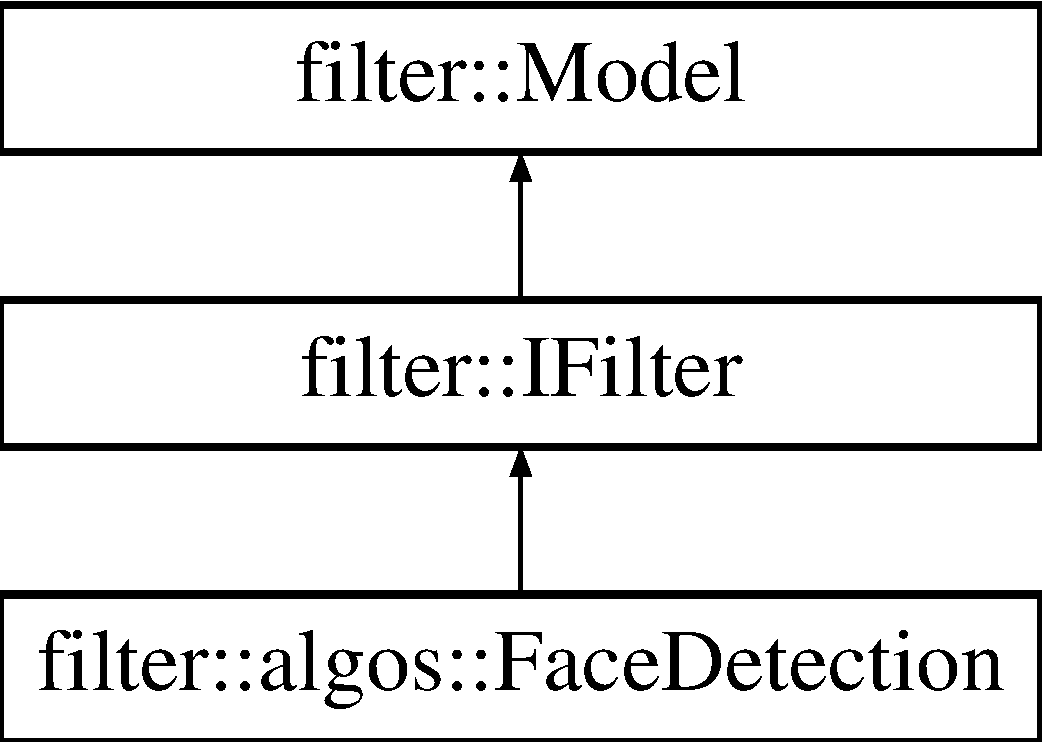
\includegraphics[height=3.000000cm]{dd/dcd/classfilter_1_1algos_1_1_face_detection}
\end{center}
\end{figure}
\subsection*{Public Types}
\begin{DoxyCompactItemize}
\item 
\mbox{\Hypertarget{classfilter_1_1algos_1_1_face_detection_a7be5df13a28b0e659f26da0181968bf1}\label{classfilter_1_1algos_1_1_face_detection_a7be5df13a28b0e659f26da0181968bf1}} 
typedef \hyperlink{class_proxy_functor}{Proxy\+Functor}$<$ \hyperlink{classfilter_1_1algos_1_1_face_detection}{Face\+Detection} $>$ {\bfseries \+\_\+proxy\+Functor}
\item 
\mbox{\Hypertarget{classfilter_1_1algos_1_1_face_detection_a1db68e3a857853eda1e62db6a661435e}\label{classfilter_1_1algos_1_1_face_detection_a1db68e3a857853eda1e62db6a661435e}} 
typedef \hyperlink{classfilter_1_1algos_1_1_face_detection}{Face\+Detection} {\bfseries mytype}
\item 
\mbox{\Hypertarget{classfilter_1_1algos_1_1_face_detection_a9f20bce236719687bb349eb2815513f0}\label{classfilter_1_1algos_1_1_face_detection_a9f20bce236719687bb349eb2815513f0}} 
typedef int {\bfseries vartype\+\_\+\+\_\+skip\+\_\+frame}
\end{DoxyCompactItemize}
\subsection*{Public Member Functions}
\begin{DoxyCompactItemize}
\item 
\mbox{\Hypertarget{classfilter_1_1algos_1_1_face_detection_af5bc7f40acdc92a682aab460105fba40}\label{classfilter_1_1algos_1_1_face_detection_af5bc7f40acdc92a682aab460105fba40}} 
void {\bfseries set\+\_\+skip\+\_\+frame\+\_\+from\+\_\+json} (boost\+::property\+\_\+tree\+::ptree \&json\+Class)
\item 
\mbox{\Hypertarget{classfilter_1_1algos_1_1_face_detection_a98e8525066ace3ed911198993317c97e}\label{classfilter_1_1algos_1_1_face_detection_a98e8525066ace3ed911198993317c97e}} 
void {\bfseries set\+\_\+skip\+\_\+frame} (vartype\+\_\+\+\_\+skip\+\_\+frame \&\+\_\+\+\_\+skip\+\_\+frame)
\item 
\mbox{\Hypertarget{classfilter_1_1algos_1_1_face_detection_a9075cc8278dcf172d30549966e69c48b}\label{classfilter_1_1algos_1_1_face_detection_a9075cc8278dcf172d30549966e69c48b}} 
vartype\+\_\+\+\_\+skip\+\_\+frame {\bfseries get\+\_\+skip\+\_\+frame} ()
\item 
\mbox{\Hypertarget{classfilter_1_1algos_1_1_face_detection_a27701697a39da6e752a78ae055ab058d}\label{classfilter_1_1algos_1_1_face_detection_a27701697a39da6e752a78ae055ab058d}} 
void {\bfseries copy\+\_\+skip\+\_\+frame} (\hyperlink{classfilter_1_1algos_1_1_face_detection}{mytype} $\ast$instance)
\item 
virtual std\+::string \hyperlink{classfilter_1_1algos_1_1_face_detection_a11c5004107d5048de93ae81ced065a26}{result\+As\+String} ()
\begin{DoxyCompactList}\small\item\em Get the result of the processing done by the node. This method will return information only. The actual processing is done by the process() method. \end{DoxyCompactList}\item 
\mbox{\Hypertarget{classfilter_1_1algos_1_1_face_detection_a4fb67105560c0886b405912cd4cedb31}\label{classfilter_1_1algos_1_1_face_detection_a4fb67105560c0886b405912cd4cedb31}} 
void \hyperlink{classfilter_1_1algos_1_1_face_detection_a4fb67105560c0886b405912cd4cedb31}{start\+Detect\+Face} ()
\begin{DoxyCompactList}\small\item\em Detects the faces in images. Runs as a separate thread. Fetch its images from the images\+Stack queue then feed the detect\+Faces method. \end{DoxyCompactList}\item 
void \hyperlink{classfilter_1_1algos_1_1_face_detection_a48cb8617d71a9827857e3d2d1e61b3f7}{detect\+Faces} (const \hyperlink{classfilter_1_1data_1_1_image_data}{data\+::\+Image\+Data} \&image)
\begin{DoxyCompactList}\small\item\em Find faces, if present, on an image. \end{DoxyCompactList}\item 
\mbox{\Hypertarget{classfilter_1_1algos_1_1_face_detection_aef784726620f237ae8988a02a8e5b16c}\label{classfilter_1_1algos_1_1_face_detection_aef784726620f237ae8988a02a8e5b16c}} 
Hipe\+Status {\bfseries process} ()
\item 
\mbox{\Hypertarget{classfilter_1_1algos_1_1_face_detection_a1d26de7e9a421f68818995e1067a49c4}\label{classfilter_1_1algos_1_1_face_detection_a1d26de7e9a421f68818995e1067a49c4}} 
virtual void {\bfseries dispose} ()
\end{DoxyCompactItemize}
\subsection*{Public Attributes}
\begin{DoxyCompactItemize}
\item 
int \hyperlink{classfilter_1_1algos_1_1_face_detection_a2dcb3e622ff24852e0c81beea2dc7681}{skip\+\_\+frame}
\end{DoxyCompactItemize}
\subsection*{Private Member Functions}
\begin{DoxyCompactItemize}
\item 
\mbox{\Hypertarget{classfilter_1_1algos_1_1_face_detection_a10ff45a1998523542d6b96a2ed126240}\label{classfilter_1_1algos_1_1_face_detection_a10ff45a1998523542d6b96a2ed126240}} 
virtual \hyperlink{classfilter_1_1data_1_1_connex_data_base}{data\+::\+Connex\+Data\+Base} \& {\bfseries get\+Connector} ()
\end{DoxyCompactItemize}
\subsection*{Private Attributes}
\begin{DoxyCompactItemize}
\item 
\mbox{\Hypertarget{classfilter_1_1algos_1_1_face_detection_abfadcb02d35c53d8a3ab28954cc314af}\label{classfilter_1_1algos_1_1_face_detection_abfadcb02d35c53d8a3ab28954cc314af}} 
int {\bfseries count\+\_\+frame}
\item 
\mbox{\Hypertarget{classfilter_1_1algos_1_1_face_detection_a8b6ccde0164cf10af292783b681879f6}\label{classfilter_1_1algos_1_1_face_detection_a8b6ccde0164cf10af292783b681879f6}} 
dlib\+::frontal\+\_\+face\+\_\+detector {\bfseries detector}
\item 
\mbox{\Hypertarget{classfilter_1_1algos_1_1_face_detection_af81d5732a898f7e0c520793fa24fe1f0}\label{classfilter_1_1algos_1_1_face_detection_af81d5732a898f7e0c520793fa24fe1f0}} 
std\+::vector$<$ dlib\+::rectangle $>$ {\bfseries dets}
\item 
\mbox{\Hypertarget{classfilter_1_1algos_1_1_face_detection_ad3c599a6092589aeba2e419593e177d4}\label{classfilter_1_1algos_1_1_face_detection_ad3c599a6092589aeba2e419593e177d4}} 
dlib\+::shape\+\_\+predictor {\bfseries pose\+\_\+model}
\item 
\mbox{\Hypertarget{classfilter_1_1algos_1_1_face_detection_a271adfc633d2083f454174d0056a3516}\label{classfilter_1_1algos_1_1_face_detection_a271adfc633d2083f454174d0056a3516}} 
std\+::atomic$<$ bool $>$ {\bfseries is\+Start}
\item 
\mbox{\Hypertarget{classfilter_1_1algos_1_1_face_detection_a5b1238db7b8e2edb5417e8d9601467f9}\label{classfilter_1_1algos_1_1_face_detection_a5b1238db7b8e2edb5417e8d9601467f9}} 
\hyperlink{classcore_1_1queue_1_1_concurrent_queue}{core\+::queue\+::\+Concurrent\+Queue}$<$ \hyperlink{classfilter_1_1data_1_1_image_data}{data\+::\+Image\+Data} $>$ {\bfseries images\+Stack}
\item 
\mbox{\Hypertarget{classfilter_1_1algos_1_1_face_detection_addc2283a606d2eea3a0a62d5d403acef}\label{classfilter_1_1algos_1_1_face_detection_addc2283a606d2eea3a0a62d5d403acef}} 
\hyperlink{classcore_1_1queue_1_1_concurrent_queue}{core\+::queue\+::\+Concurrent\+Queue}$<$ \hyperlink{classfilter_1_1data_1_1_square_crop}{data\+::\+Square\+Crop} $>$ {\bfseries crops}
\item 
\mbox{\Hypertarget{classfilter_1_1algos_1_1_face_detection_a938767be5946dead5970c667b5164043}\label{classfilter_1_1algos_1_1_face_detection_a938767be5946dead5970c667b5164043}} 
\hyperlink{classfilter_1_1data_1_1_square_crop}{data\+::\+Square\+Crop} {\bfseries tosend}
\item 
\mbox{\Hypertarget{classfilter_1_1algos_1_1_face_detection_add5efbfa77b142f82bcc00cc6a1a5d91}\label{classfilter_1_1algos_1_1_face_detection_add5efbfa77b142f82bcc00cc6a1a5d91}} 
boost\+::thread $\ast$ {\bfseries thr\+\_\+server}
\item 
\mbox{\Hypertarget{classfilter_1_1algos_1_1_face_detection_a7a24695a45fe28450274c5c179bb844a}\label{classfilter_1_1algos_1_1_face_detection_a7a24695a45fe28450274c5c179bb844a}} 
\hyperlink{classfilter_1_1data_1_1_connex_data}{data\+::\+Connex\+Data}$<$ \hyperlink{classfilter_1_1data_1_1_image_array_data}{data\+::\+Image\+Array\+Data}, \hyperlink{classfilter_1_1data_1_1_square_crop}{data\+::\+Square\+Crop} $>$ {\bfseries \+\_\+connex\+Data}
\end{DoxyCompactItemize}
\subsection*{Additional Inherited Members}


\subsection{Detailed Description}
\begin{DoxyRefDesc}{Todo}
\item[\hyperlink{todo__todo000008}{Todo}]\end{DoxyRefDesc}
The filter uses dlib. It will output a Square\+Crop object containing all the found faces. 

\subsection{Member Function Documentation}
\mbox{\Hypertarget{classfilter_1_1algos_1_1_face_detection_a48cb8617d71a9827857e3d2d1e61b3f7}\label{classfilter_1_1algos_1_1_face_detection_a48cb8617d71a9827857e3d2d1e61b3f7}} 
\index{filter\+::algos\+::\+Face\+Detection@{filter\+::algos\+::\+Face\+Detection}!detect\+Faces@{detect\+Faces}}
\index{detect\+Faces@{detect\+Faces}!filter\+::algos\+::\+Face\+Detection@{filter\+::algos\+::\+Face\+Detection}}
\subsubsection{\texorpdfstring{detect\+Faces()}{detectFaces()}}
{\footnotesize\ttfamily void filter\+::algos\+::\+Face\+Detection\+::detect\+Faces (\begin{DoxyParamCaption}\item[{const \hyperlink{classfilter_1_1data_1_1_image_data}{data\+::\+Image\+Data} \&}]{image }\end{DoxyParamCaption})}


\begin{DoxyParams}{Parameters}
{\em image} & The image to process and on which we\textquotesingle{}ll try to find faces. \\
\hline
\end{DoxyParams}
\mbox{\Hypertarget{classfilter_1_1algos_1_1_face_detection_a11c5004107d5048de93ae81ced065a26}\label{classfilter_1_1algos_1_1_face_detection_a11c5004107d5048de93ae81ced065a26}} 
\index{filter\+::algos\+::\+Face\+Detection@{filter\+::algos\+::\+Face\+Detection}!result\+As\+String@{result\+As\+String}}
\index{result\+As\+String@{result\+As\+String}!filter\+::algos\+::\+Face\+Detection@{filter\+::algos\+::\+Face\+Detection}}
\subsubsection{\texorpdfstring{result\+As\+String()}{resultAsString()}}
{\footnotesize\ttfamily virtual std\+::string filter\+::algos\+::\+Face\+Detection\+::result\+As\+String (\begin{DoxyParamCaption}{ }\end{DoxyParamCaption})\hspace{0.3cm}{\ttfamily [inline]}, {\ttfamily [virtual]}}

\begin{DoxyReturn}{Returns}
A string containing the result of the processing done by the filter. 
\end{DoxyReturn}


Reimplemented from \hyperlink{classfilter_1_1_i_filter_ab99902b060a6d9edc3452a8c9f85e37e}{filter\+::\+I\+Filter}.



\subsection{Member Data Documentation}
\mbox{\Hypertarget{classfilter_1_1algos_1_1_face_detection_a2dcb3e622ff24852e0c81beea2dc7681}\label{classfilter_1_1algos_1_1_face_detection_a2dcb3e622ff24852e0c81beea2dc7681}} 
\index{filter\+::algos\+::\+Face\+Detection@{filter\+::algos\+::\+Face\+Detection}!skip\+\_\+frame@{skip\+\_\+frame}}
\index{skip\+\_\+frame@{skip\+\_\+frame}!filter\+::algos\+::\+Face\+Detection@{filter\+::algos\+::\+Face\+Detection}}
\subsubsection{\texorpdfstring{skip\+\_\+frame}{skip\_frame}}
{\footnotesize\ttfamily filter\+::algos\+::\+Face\+Detection\+::skip\+\_\+frame}

The number of frames to skip between each detection. 

The documentation for this class was generated from the following files\+:\begin{DoxyCompactItemize}
\item 
header/filter/\+Algos/Face\+Detection.\+h\item 
source/filter/algos/Face\+Detection.\+cpp\end{DoxyCompactItemize}

\hypertarget{classfilter_1_1algos_1_1_face_landmark}{}\section{filter\+:\+:algos\+:\+:Face\+Landmark Class Reference}
\label{classfilter_1_1algos_1_1_face_landmark}\index{filter\+::algos\+::\+Face\+Landmark@{filter\+::algos\+::\+Face\+Landmark}}


The \hyperlink{classfilter_1_1algos_1_1_face_landmark}{Face\+Landmark} filter will find the faces and their landmarks.  




{\ttfamily \#include $<$Face\+Landmark.\+h$>$}

Inheritance diagram for filter\+:\+:algos\+:\+:Face\+Landmark\+:\begin{figure}[H]
\begin{center}
\leavevmode
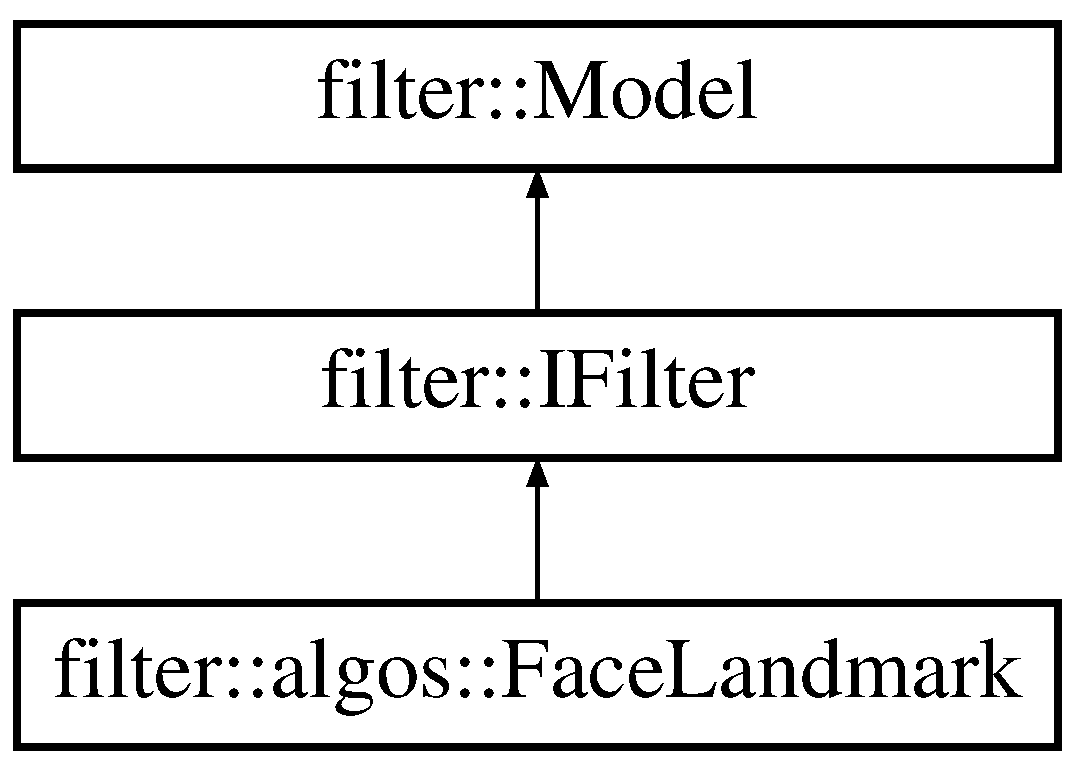
\includegraphics[height=3.000000cm]{dc/d8b/classfilter_1_1algos_1_1_face_landmark}
\end{center}
\end{figure}
\subsection*{Public Types}
\begin{DoxyCompactItemize}
\item 
\mbox{\Hypertarget{classfilter_1_1algos_1_1_face_landmark_ab916a495ad33d6879b0516210673981b}\label{classfilter_1_1algos_1_1_face_landmark_ab916a495ad33d6879b0516210673981b}} 
typedef \hyperlink{class_proxy_functor}{Proxy\+Functor}$<$ \hyperlink{classfilter_1_1algos_1_1_face_landmark}{Face\+Landmark} $>$ {\bfseries \+\_\+proxy\+Functor}
\item 
\mbox{\Hypertarget{classfilter_1_1algos_1_1_face_landmark_ac4503704d0dc53e61e40935f9584d5d1}\label{classfilter_1_1algos_1_1_face_landmark_ac4503704d0dc53e61e40935f9584d5d1}} 
typedef \hyperlink{classfilter_1_1algos_1_1_face_landmark}{Face\+Landmark} {\bfseries mytype}
\item 
\mbox{\Hypertarget{classfilter_1_1algos_1_1_face_landmark_a8d83414d1c84d98963889c2bbeabc9c7}\label{classfilter_1_1algos_1_1_face_landmark_a8d83414d1c84d98963889c2bbeabc9c7}} 
typedef int {\bfseries vartype\+\_\+\+\_\+skip\+\_\+frame}
\end{DoxyCompactItemize}
\subsection*{Public Member Functions}
\begin{DoxyCompactItemize}
\item 
\mbox{\Hypertarget{classfilter_1_1algos_1_1_face_landmark_aeb2c21e10e7f75419f36057b4d939bea}\label{classfilter_1_1algos_1_1_face_landmark_aeb2c21e10e7f75419f36057b4d939bea}} 
void {\bfseries set\+\_\+skip\+\_\+frame\+\_\+from\+\_\+json} (boost\+::property\+\_\+tree\+::ptree \&json\+Class)
\item 
\mbox{\Hypertarget{classfilter_1_1algos_1_1_face_landmark_a28e8e33777606e43275cfafe3aebcc05}\label{classfilter_1_1algos_1_1_face_landmark_a28e8e33777606e43275cfafe3aebcc05}} 
void {\bfseries set\+\_\+skip\+\_\+frame} (vartype\+\_\+\+\_\+skip\+\_\+frame \&\+\_\+\+\_\+skip\+\_\+frame)
\item 
\mbox{\Hypertarget{classfilter_1_1algos_1_1_face_landmark_ab681a83019eadfd6602896c023232858}\label{classfilter_1_1algos_1_1_face_landmark_ab681a83019eadfd6602896c023232858}} 
vartype\+\_\+\+\_\+skip\+\_\+frame {\bfseries get\+\_\+skip\+\_\+frame} ()
\item 
\mbox{\Hypertarget{classfilter_1_1algos_1_1_face_landmark_a423be6eed67a3655a82a21586de7402f}\label{classfilter_1_1algos_1_1_face_landmark_a423be6eed67a3655a82a21586de7402f}} 
void {\bfseries copy\+\_\+skip\+\_\+frame} (\hyperlink{classfilter_1_1algos_1_1_face_landmark}{mytype} $\ast$instance)
\item 
virtual std\+::string \hyperlink{classfilter_1_1algos_1_1_face_landmark_a58eca9d87717bac1696c2b008af4342a}{result\+As\+String} ()
\begin{DoxyCompactList}\small\item\em Get the result of the processing done by the node. This method will return information only. The actual processing is done by the process() method. \end{DoxyCompactList}\item 
\mbox{\Hypertarget{classfilter_1_1algos_1_1_face_landmark_a09244ac23fa2ba1c7a22c1a145cc9d58}\label{classfilter_1_1algos_1_1_face_landmark_a09244ac23fa2ba1c7a22c1a145cc9d58}} 
void \hyperlink{classfilter_1_1algos_1_1_face_landmark_a09244ac23fa2ba1c7a22c1a145cc9d58}{start\+Detect\+Face} ()
\begin{DoxyCompactList}\small\item\em Detects the faces in images. Runs as a separate thread. Fetch its images from the images\+Stack queue then feed the detect\+Faces method. \end{DoxyCompactList}\item 
cv\+::\+Mat \hyperlink{classfilter_1_1algos_1_1_face_landmark_a333f1eb7faccf486e00d654a0f396ae9}{detect\+Faces} (const \hyperlink{classfilter_1_1data_1_1_image_data}{data\+::\+Image\+Data} \&image)
\begin{DoxyCompactList}\small\item\em Find faces, if present, then their landmarks. \end{DoxyCompactList}\item 
\mbox{\Hypertarget{classfilter_1_1algos_1_1_face_landmark_ab6d4e7beca4ddd5f09ee927cfe6914b3}\label{classfilter_1_1algos_1_1_face_landmark_ab6d4e7beca4ddd5f09ee927cfe6914b3}} 
Hipe\+Status {\bfseries process} ()
\item 
\mbox{\Hypertarget{classfilter_1_1algos_1_1_face_landmark_ad1c9348a4d7ada38562bab0371d92b8d}\label{classfilter_1_1algos_1_1_face_landmark_ad1c9348a4d7ada38562bab0371d92b8d}} 
virtual void {\bfseries dispose} ()
\end{DoxyCompactItemize}
\subsection*{Public Attributes}
\begin{DoxyCompactItemize}
\item 
int \hyperlink{classfilter_1_1algos_1_1_face_landmark_a6fe568dc4782d0e560947dab7417dab4}{skip\+\_\+frame}
\end{DoxyCompactItemize}
\subsection*{Private Member Functions}
\begin{DoxyCompactItemize}
\item 
\mbox{\Hypertarget{classfilter_1_1algos_1_1_face_landmark_acf6eac334b8f03dea88ff93b1ab03270}\label{classfilter_1_1algos_1_1_face_landmark_acf6eac334b8f03dea88ff93b1ab03270}} 
virtual \hyperlink{classfilter_1_1data_1_1_connex_data_base}{data\+::\+Connex\+Data\+Base} \& {\bfseries get\+Connector} ()
\end{DoxyCompactItemize}
\subsection*{Private Attributes}
\begin{DoxyCompactItemize}
\item 
\mbox{\Hypertarget{classfilter_1_1algos_1_1_face_landmark_a77081eb7fa985cbf60c16189c55a3bbd}\label{classfilter_1_1algos_1_1_face_landmark_a77081eb7fa985cbf60c16189c55a3bbd}} 
int {\bfseries count\+\_\+frame}
\item 
\mbox{\Hypertarget{classfilter_1_1algos_1_1_face_landmark_a1a04ccd050f78322da687211f3f96097}\label{classfilter_1_1algos_1_1_face_landmark_a1a04ccd050f78322da687211f3f96097}} 
dlib\+::frontal\+\_\+face\+\_\+detector {\bfseries detector}
\item 
\mbox{\Hypertarget{classfilter_1_1algos_1_1_face_landmark_a69287e3b5462a96e991a222d3ff328e3}\label{classfilter_1_1algos_1_1_face_landmark_a69287e3b5462a96e991a222d3ff328e3}} 
std\+::vector$<$ dlib\+::rectangle $>$ {\bfseries dets}
\item 
\mbox{\Hypertarget{classfilter_1_1algos_1_1_face_landmark_a2d9af3baf74a483045047667a2260d0b}\label{classfilter_1_1algos_1_1_face_landmark_a2d9af3baf74a483045047667a2260d0b}} 
dlib\+::shape\+\_\+predictor {\bfseries pose\+\_\+model}
\item 
\mbox{\Hypertarget{classfilter_1_1algos_1_1_face_landmark_a74a80b682e53b82946844575bf9c8d2f}\label{classfilter_1_1algos_1_1_face_landmark_a74a80b682e53b82946844575bf9c8d2f}} 
std\+::atomic$<$ bool $>$ {\bfseries is\+Start}
\item 
\mbox{\Hypertarget{classfilter_1_1algos_1_1_face_landmark_a7b114dda5095aa783b1bf165a6d3fc4d}\label{classfilter_1_1algos_1_1_face_landmark_a7b114dda5095aa783b1bf165a6d3fc4d}} 
\hyperlink{classcore_1_1queue_1_1_concurrent_queue}{core\+::queue\+::\+Concurrent\+Queue}$<$ \hyperlink{classfilter_1_1data_1_1_image_data}{data\+::\+Image\+Data} $>$ {\bfseries images\+Stack}
\item 
\mbox{\Hypertarget{classfilter_1_1algos_1_1_face_landmark_acd6ae34d87edf76630b9641753ab6859}\label{classfilter_1_1algos_1_1_face_landmark_acd6ae34d87edf76630b9641753ab6859}} 
\hyperlink{classcore_1_1queue_1_1_concurrent_queue}{core\+::queue\+::\+Concurrent\+Queue}$<$ \hyperlink{classfilter_1_1data_1_1_image_data}{data\+::\+Image\+Data} $>$ {\bfseries shapes}
\item 
\mbox{\Hypertarget{classfilter_1_1algos_1_1_face_landmark_a94727dd37708c46475d62eecb236622c}\label{classfilter_1_1algos_1_1_face_landmark_a94727dd37708c46475d62eecb236622c}} 
\hyperlink{classfilter_1_1data_1_1_image_data}{data\+::\+Image\+Data} {\bfseries tosend}
\item 
\mbox{\Hypertarget{classfilter_1_1algos_1_1_face_landmark_a7051048368fc84b6361b484171596684}\label{classfilter_1_1algos_1_1_face_landmark_a7051048368fc84b6361b484171596684}} 
boost\+::thread $\ast$ {\bfseries thr\+\_\+server}
\item 
\mbox{\Hypertarget{classfilter_1_1algos_1_1_face_landmark_aa9074b9b1af3d43bdc61aae926a144f5}\label{classfilter_1_1algos_1_1_face_landmark_aa9074b9b1af3d43bdc61aae926a144f5}} 
\hyperlink{classfilter_1_1data_1_1_connex_data}{data\+::\+Connex\+Data}$<$ \hyperlink{classfilter_1_1data_1_1_image_array_data}{data\+::\+Image\+Array\+Data}, \hyperlink{classfilter_1_1data_1_1_image_data}{data\+::\+Image\+Data} $>$ {\bfseries \+\_\+connex\+Data}
\end{DoxyCompactItemize}
\subsection*{Additional Inherited Members}


\subsection{Detailed Description}
\begin{DoxyRefDesc}{Todo}
\item[\hyperlink{todo__todo000009}{Todo}]\end{DoxyRefDesc}
The landmarks are the keypoints needed to identify the facial expression. 

\subsection{Member Function Documentation}
\mbox{\Hypertarget{classfilter_1_1algos_1_1_face_landmark_a333f1eb7faccf486e00d654a0f396ae9}\label{classfilter_1_1algos_1_1_face_landmark_a333f1eb7faccf486e00d654a0f396ae9}} 
\index{filter\+::algos\+::\+Face\+Landmark@{filter\+::algos\+::\+Face\+Landmark}!detect\+Faces@{detect\+Faces}}
\index{detect\+Faces@{detect\+Faces}!filter\+::algos\+::\+Face\+Landmark@{filter\+::algos\+::\+Face\+Landmark}}
\subsubsection{\texorpdfstring{detect\+Faces()}{detectFaces()}}
{\footnotesize\ttfamily cv\+::\+Mat filter\+::algos\+::\+Face\+Landmark\+::detect\+Faces (\begin{DoxyParamCaption}\item[{const \hyperlink{classfilter_1_1data_1_1_image_data}{data\+::\+Image\+Data} \&}]{image }\end{DoxyParamCaption})}


\begin{DoxyParams}{Parameters}
{\em image} & The image to process to try finding faces. \\
\hline
\end{DoxyParams}
\begin{DoxyReturn}{Returns}
Returns the processed frame with the landmarks of the found faces drawn on it. 
\end{DoxyReturn}
\mbox{\Hypertarget{classfilter_1_1algos_1_1_face_landmark_a58eca9d87717bac1696c2b008af4342a}\label{classfilter_1_1algos_1_1_face_landmark_a58eca9d87717bac1696c2b008af4342a}} 
\index{filter\+::algos\+::\+Face\+Landmark@{filter\+::algos\+::\+Face\+Landmark}!result\+As\+String@{result\+As\+String}}
\index{result\+As\+String@{result\+As\+String}!filter\+::algos\+::\+Face\+Landmark@{filter\+::algos\+::\+Face\+Landmark}}
\subsubsection{\texorpdfstring{result\+As\+String()}{resultAsString()}}
{\footnotesize\ttfamily virtual std\+::string filter\+::algos\+::\+Face\+Landmark\+::result\+As\+String (\begin{DoxyParamCaption}{ }\end{DoxyParamCaption})\hspace{0.3cm}{\ttfamily [inline]}, {\ttfamily [virtual]}}

\begin{DoxyReturn}{Returns}
A string containing the result of the processing done by the filter. 
\end{DoxyReturn}


Reimplemented from \hyperlink{classfilter_1_1_i_filter_ab99902b060a6d9edc3452a8c9f85e37e}{filter\+::\+I\+Filter}.



\subsection{Member Data Documentation}
\mbox{\Hypertarget{classfilter_1_1algos_1_1_face_landmark_a6fe568dc4782d0e560947dab7417dab4}\label{classfilter_1_1algos_1_1_face_landmark_a6fe568dc4782d0e560947dab7417dab4}} 
\index{filter\+::algos\+::\+Face\+Landmark@{filter\+::algos\+::\+Face\+Landmark}!skip\+\_\+frame@{skip\+\_\+frame}}
\index{skip\+\_\+frame@{skip\+\_\+frame}!filter\+::algos\+::\+Face\+Landmark@{filter\+::algos\+::\+Face\+Landmark}}
\subsubsection{\texorpdfstring{skip\+\_\+frame}{skip\_frame}}
{\footnotesize\ttfamily filter\+::algos\+::\+Face\+Landmark\+::skip\+\_\+frame}

The number of frames to skip between each detection. 

The documentation for this class was generated from the following files\+:\begin{DoxyCompactItemize}
\item 
header/filter/\+Algos/Face\+Landmark.\+h\item 
source/filter/algos/Face\+Landmark.\+cpp\end{DoxyCompactItemize}

\hypertarget{class_m_e_s_a_i_1_1_f_fmpeg_decoder}{}\section{M\+E\+S\+AI\+:\+:F\+Fmpeg\+Decoder Class Reference}
\label{class_m_e_s_a_i_1_1_f_fmpeg_decoder}\index{M\+E\+S\+A\+I\+::\+F\+Fmpeg\+Decoder@{M\+E\+S\+A\+I\+::\+F\+Fmpeg\+Decoder}}
Inheritance diagram for M\+E\+S\+AI\+:\+:F\+Fmpeg\+Decoder\+:\begin{figure}[H]
\begin{center}
\leavevmode
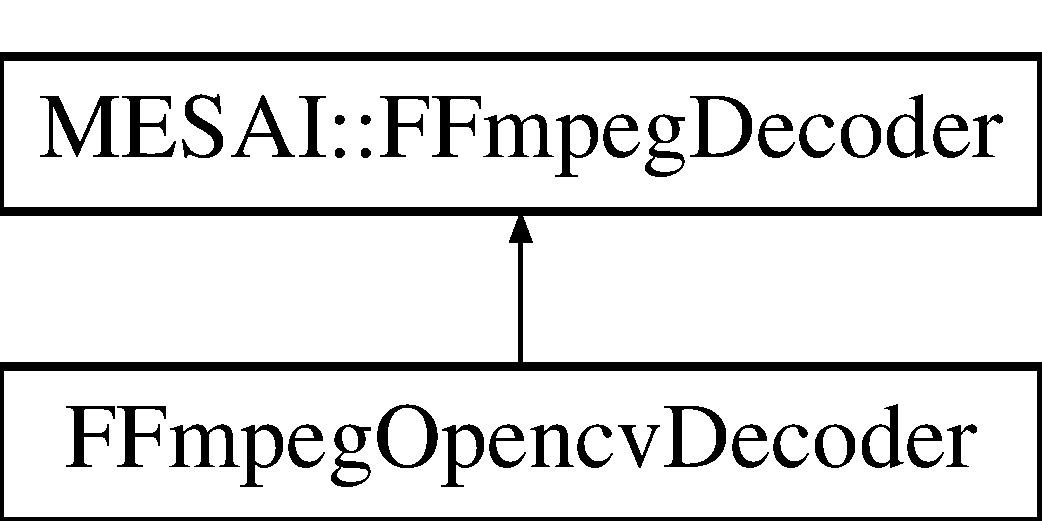
\includegraphics[height=2.000000cm]{d2/dfc/class_m_e_s_a_i_1_1_f_fmpeg_decoder}
\end{center}
\end{figure}
\subsection*{Public Member Functions}
\begin{DoxyCompactItemize}
\item 
\mbox{\Hypertarget{class_m_e_s_a_i_1_1_f_fmpeg_decoder_a7ebd1c86816d9510c993c453c2a26d90}\label{class_m_e_s_a_i_1_1_f_fmpeg_decoder_a7ebd1c86816d9510c993c453c2a26d90}} 
{\bfseries F\+Fmpeg\+Decoder} (std\+::string)
\item 
\mbox{\Hypertarget{class_m_e_s_a_i_1_1_f_fmpeg_decoder_ad7d30c2c905e1c46e12744ec39937305}\label{class_m_e_s_a_i_1_1_f_fmpeg_decoder_ad7d30c2c905e1c46e12744ec39937305}} 
virtual void {\bfseries intialize} ()
\item 
\mbox{\Hypertarget{class_m_e_s_a_i_1_1_f_fmpeg_decoder_a2b3b9e74c202fbe852d9e09ee467b175}\label{class_m_e_s_a_i_1_1_f_fmpeg_decoder_a2b3b9e74c202fbe852d9e09ee467b175}} 
virtual void {\bfseries play\+Media} ()
\item 
\mbox{\Hypertarget{class_m_e_s_a_i_1_1_f_fmpeg_decoder_a8a6ac425e188fbd2ff68c5a43e0d24a6}\label{class_m_e_s_a_i_1_1_f_fmpeg_decoder_a8a6ac425e188fbd2ff68c5a43e0d24a6}} 
virtual void {\bfseries finalize} ()
\item 
\mbox{\Hypertarget{class_m_e_s_a_i_1_1_f_fmpeg_decoder_ac1da1b4a9db30b2027a1c9a9821f7b28}\label{class_m_e_s_a_i_1_1_f_fmpeg_decoder_ac1da1b4a9db30b2027a1c9a9821f7b28}} 
void {\bfseries set\+Onframe\+Callback\+Function} (std\+::function$<$ void(cv\+::\+Mat \&)$>$ func)
\end{DoxyCompactItemize}
\subsection*{Public Attributes}
\begin{DoxyCompactItemize}
\item 
\mbox{\Hypertarget{class_m_e_s_a_i_1_1_f_fmpeg_decoder_a573ebc8ff1e2fdb34d25dc43491ef8f5}\label{class_m_e_s_a_i_1_1_f_fmpeg_decoder_a573ebc8ff1e2fdb34d25dc43491ef8f5}} 
int {\bfseries width}
\item 
\mbox{\Hypertarget{class_m_e_s_a_i_1_1_f_fmpeg_decoder_a21ce7c6c31abdfdcfbb3ec19fcb7b24e}\label{class_m_e_s_a_i_1_1_f_fmpeg_decoder_a21ce7c6c31abdfdcfbb3ec19fcb7b24e}} 
int {\bfseries height}
\item 
\mbox{\Hypertarget{class_m_e_s_a_i_1_1_f_fmpeg_decoder_ad727d8ba3ca73d9837d703018c335a6c}\label{class_m_e_s_a_i_1_1_f_fmpeg_decoder_ad727d8ba3ca73d9837d703018c335a6c}} 
int {\bfseries G\+OP}
\item 
\mbox{\Hypertarget{class_m_e_s_a_i_1_1_f_fmpeg_decoder_a59bee3ac056dd0d6c8fdb3c6f6a6b74f}\label{class_m_e_s_a_i_1_1_f_fmpeg_decoder_a59bee3ac056dd0d6c8fdb3c6f6a6b74f}} 
int {\bfseries frame\+Rate}
\item 
\mbox{\Hypertarget{class_m_e_s_a_i_1_1_f_fmpeg_decoder_a0a06c5a6670dabda8d571f65101a75cd}\label{class_m_e_s_a_i_1_1_f_fmpeg_decoder_a0a06c5a6670dabda8d571f65101a75cd}} 
int {\bfseries bitrate}
\item 
\mbox{\Hypertarget{class_m_e_s_a_i_1_1_f_fmpeg_decoder_a17913d19b2d877998d7bba9b5801a1ad}\label{class_m_e_s_a_i_1_1_f_fmpeg_decoder_a17913d19b2d877998d7bba9b5801a1ad}} 
std\+::function$<$ void(cv\+::\+Mat \&)$>$ {\bfseries on\+Frame}
\end{DoxyCompactItemize}
\subsection*{Protected Attributes}
\begin{DoxyCompactItemize}
\item 
\mbox{\Hypertarget{class_m_e_s_a_i_1_1_f_fmpeg_decoder_a04c74d07cfc273de1f6cc719c4560830}\label{class_m_e_s_a_i_1_1_f_fmpeg_decoder_a04c74d07cfc273de1f6cc719c4560830}} 
std\+::string {\bfseries path}
\item 
\mbox{\Hypertarget{class_m_e_s_a_i_1_1_f_fmpeg_decoder_abdd6372101e492c581be900e600f4eec}\label{class_m_e_s_a_i_1_1_f_fmpeg_decoder_abdd6372101e492c581be900e600f4eec}} 
A\+V\+Codec\+Context $\ast$ {\bfseries p\+Codec\+Ctx}
\item 
\mbox{\Hypertarget{class_m_e_s_a_i_1_1_f_fmpeg_decoder_a514e4015809c9fea0553b256b2b1ed47}\label{class_m_e_s_a_i_1_1_f_fmpeg_decoder_a514e4015809c9fea0553b256b2b1ed47}} 
A\+V\+Format\+Context $\ast$ {\bfseries p\+Format\+Ctx}
\item 
\mbox{\Hypertarget{class_m_e_s_a_i_1_1_f_fmpeg_decoder_a1ea3e6e36bf3949b1821b9801a028310}\label{class_m_e_s_a_i_1_1_f_fmpeg_decoder_a1ea3e6e36bf3949b1821b9801a028310}} 
A\+V\+Frame $\ast$ {\bfseries p\+Frame\+R\+GB}
\item 
\mbox{\Hypertarget{class_m_e_s_a_i_1_1_f_fmpeg_decoder_a6a1d6f5e64e0559629385f53119e7768}\label{class_m_e_s_a_i_1_1_f_fmpeg_decoder_a6a1d6f5e64e0559629385f53119e7768}} 
struct Sws\+Context $\ast$ {\bfseries img\+\_\+convert\+\_\+ctx}
\item 
\mbox{\Hypertarget{class_m_e_s_a_i_1_1_f_fmpeg_decoder_a825efecc65e8731d027779ee56cc633d}\label{class_m_e_s_a_i_1_1_f_fmpeg_decoder_a825efecc65e8731d027779ee56cc633d}} 
int {\bfseries video\+Stream}
\end{DoxyCompactItemize}


The documentation for this class was generated from the following files\+:\begin{DoxyCompactItemize}
\item 
header/streaming\+\_\+rtsp/F\+Fmpeg\+Decoder.\+h\item 
source/streaming\+\_\+rtsp/F\+Fmpeg\+Decoder.\+cpp\end{DoxyCompactItemize}

\hypertarget{class_m_e_s_a_i_1_1_f_fmpeg_h264_encoder}{}\section{M\+E\+S\+AI\+:\+:F\+Fmpeg\+H264\+Encoder Class Reference}
\label{class_m_e_s_a_i_1_1_f_fmpeg_h264_encoder}\index{M\+E\+S\+A\+I\+::\+F\+Fmpeg\+H264\+Encoder@{M\+E\+S\+A\+I\+::\+F\+Fmpeg\+H264\+Encoder}}
\subsection*{Public Member Functions}
\begin{DoxyCompactItemize}
\item 
\mbox{\Hypertarget{class_m_e_s_a_i_1_1_f_fmpeg_h264_encoder_a242e5d0e654b8f83ca033e637208d0aa}\label{class_m_e_s_a_i_1_1_f_fmpeg_h264_encoder_a242e5d0e654b8f83ca033e637208d0aa}} 
void {\bfseries set\+Callback\+Function\+Frame\+Is\+Ready} (std\+::function$<$ void()$>$ func)
\item 
\mbox{\Hypertarget{class_m_e_s_a_i_1_1_f_fmpeg_h264_encoder_a14d986ee397f53950a1dce392c942276}\label{class_m_e_s_a_i_1_1_f_fmpeg_h264_encoder_a14d986ee397f53950a1dce392c942276}} 
void {\bfseries convert\+Image\+Mult2} (cv\+::\+Mat \&image)
\item 
\mbox{\Hypertarget{class_m_e_s_a_i_1_1_f_fmpeg_h264_encoder_a6a84030b147c3b888e0a4748ceefd0d6}\label{class_m_e_s_a_i_1_1_f_fmpeg_h264_encoder_a6a84030b147c3b888e0a4748ceefd0d6}} 
void {\bfseries Setup\+Video} (std\+::string filename, int Width, int Height, int F\+PS, int G\+OB, int Bit\+Per\+Second)
\item 
\mbox{\Hypertarget{class_m_e_s_a_i_1_1_f_fmpeg_h264_encoder_a5af225d104a7a503c051a1b2275c0bc5}\label{class_m_e_s_a_i_1_1_f_fmpeg_h264_encoder_a5af225d104a7a503c051a1b2275c0bc5}} 
void {\bfseries Close\+Video} ()
\item 
\mbox{\Hypertarget{class_m_e_s_a_i_1_1_f_fmpeg_h264_encoder_a47a9fee0cf51cf294a939e3778db407d}\label{class_m_e_s_a_i_1_1_f_fmpeg_h264_encoder_a47a9fee0cf51cf294a939e3778db407d}} 
void {\bfseries Setup\+Codec} (const char $\ast$filename, int codec\+\_\+id)
\item 
\mbox{\Hypertarget{class_m_e_s_a_i_1_1_f_fmpeg_h264_encoder_a5031f20ba6f4a948a2e1f5aab19fd223}\label{class_m_e_s_a_i_1_1_f_fmpeg_h264_encoder_a5031f20ba6f4a948a2e1f5aab19fd223}} 
void {\bfseries Close\+Codec} ()
\item 
\mbox{\Hypertarget{class_m_e_s_a_i_1_1_f_fmpeg_h264_encoder_a31d211927f361f73ea76c8fabf955baf}\label{class_m_e_s_a_i_1_1_f_fmpeg_h264_encoder_a31d211927f361f73ea76c8fabf955baf}} 
void {\bfseries Send\+New\+Frame} (cv\+::\+Mat R\+G\+B\+Frame)
\item 
\mbox{\Hypertarget{class_m_e_s_a_i_1_1_f_fmpeg_h264_encoder_acc8ed78ccf68e30d30ebb62565de11c3}\label{class_m_e_s_a_i_1_1_f_fmpeg_h264_encoder_acc8ed78ccf68e30d30ebb62565de11c3}} 
void {\bfseries Write\+Frame} (cv\+::\+Mat \&R\+G\+B\+Frame)
\item 
\mbox{\Hypertarget{class_m_e_s_a_i_1_1_f_fmpeg_h264_encoder_aa42834033f0fba672020bc510a9739c2}\label{class_m_e_s_a_i_1_1_f_fmpeg_h264_encoder_aa42834033f0fba672020bc510a9739c2}} 
char {\bfseries Release\+Frame} ()
\item 
\mbox{\Hypertarget{class_m_e_s_a_i_1_1_f_fmpeg_h264_encoder_a876d1dc5406ce3a427b4d31bba2fb163}\label{class_m_e_s_a_i_1_1_f_fmpeg_h264_encoder_a876d1dc5406ce3a427b4d31bba2fb163}} 
void {\bfseries run} ()
\item 
\mbox{\Hypertarget{class_m_e_s_a_i_1_1_f_fmpeg_h264_encoder_a5614f1f368de7abba534e7517a493310}\label{class_m_e_s_a_i_1_1_f_fmpeg_h264_encoder_a5614f1f368de7abba534e7517a493310}} 
char {\bfseries Get\+Frame} (uint8\+\_\+t $\ast$$\ast$Frame\+Buffer, unsigned int $\ast$Frame\+Size)
\end{DoxyCompactItemize}
\subsection*{Public Attributes}
\begin{DoxyCompactItemize}
\item 
\mbox{\Hypertarget{class_m_e_s_a_i_1_1_f_fmpeg_h264_encoder_ae90e54edfbbc3341fcebe8f9345d7f4b}\label{class_m_e_s_a_i_1_1_f_fmpeg_h264_encoder_ae90e54edfbbc3341fcebe8f9345d7f4b}} 
std\+::atomic$<$ bool $>$ {\bfseries quit}
\end{DoxyCompactItemize}
\subsection*{Private Attributes}
\begin{DoxyCompactItemize}
\item 
\mbox{\Hypertarget{class_m_e_s_a_i_1_1_f_fmpeg_h264_encoder_ad2da2c1360276b7cb48433f9d5c1c065}\label{class_m_e_s_a_i_1_1_f_fmpeg_h264_encoder_ad2da2c1360276b7cb48433f9d5c1c065}} 
std\+::queue$<$ cv\+::\+Mat $>$ {\bfseries inqueue}
\item 
\mbox{\Hypertarget{class_m_e_s_a_i_1_1_f_fmpeg_h264_encoder_a26fa81f02105bc7b2bdc8628d501fac4}\label{class_m_e_s_a_i_1_1_f_fmpeg_h264_encoder_a26fa81f02105bc7b2bdc8628d501fac4}} 
std\+::mutex {\bfseries inqueue\+\_\+mutex}
\item 
\mbox{\Hypertarget{class_m_e_s_a_i_1_1_f_fmpeg_h264_encoder_a74d8aa3acf32228262764dc255db4a1c}\label{class_m_e_s_a_i_1_1_f_fmpeg_h264_encoder_a74d8aa3acf32228262764dc255db4a1c}} 
std\+::queue$<$ \hyperlink{class_m_e_s_a_i_1_1_frame_structure}{Frame\+Structure} $\ast$ $>$ {\bfseries outqueue}
\item 
\mbox{\Hypertarget{class_m_e_s_a_i_1_1_f_fmpeg_h264_encoder_a1da76b5e28e09492339625ac6510964f}\label{class_m_e_s_a_i_1_1_f_fmpeg_h264_encoder_a1da76b5e28e09492339625ac6510964f}} 
std\+::mutex {\bfseries outqueue\+\_\+mutex}
\item 
\mbox{\Hypertarget{class_m_e_s_a_i_1_1_f_fmpeg_h264_encoder_a789338488d109415d654a4f13edff014}\label{class_m_e_s_a_i_1_1_f_fmpeg_h264_encoder_a789338488d109415d654a4f13edff014}} 
int {\bfseries m\+\_\+sws\+\_\+flags}
\item 
\mbox{\Hypertarget{class_m_e_s_a_i_1_1_f_fmpeg_h264_encoder_a4dda85e0b2319a0870ea72b54aa555ad}\label{class_m_e_s_a_i_1_1_f_fmpeg_h264_encoder_a4dda85e0b2319a0870ea72b54aa555ad}} 
int {\bfseries m\+\_\+\+A\+V\+I\+M\+O\+V\+\_\+\+F\+PS}
\item 
\mbox{\Hypertarget{class_m_e_s_a_i_1_1_f_fmpeg_h264_encoder_a9398ebdfb7954a953a988153758d3734}\label{class_m_e_s_a_i_1_1_f_fmpeg_h264_encoder_a9398ebdfb7954a953a988153758d3734}} 
int {\bfseries m\+\_\+\+A\+V\+I\+M\+O\+V\+\_\+\+G\+OB}
\item 
\mbox{\Hypertarget{class_m_e_s_a_i_1_1_f_fmpeg_h264_encoder_a5abcfa309a22e69a22311526499e5ff2}\label{class_m_e_s_a_i_1_1_f_fmpeg_h264_encoder_a5abcfa309a22e69a22311526499e5ff2}} 
int {\bfseries m\+\_\+\+A\+V\+I\+M\+O\+V\+\_\+\+B\+PS}
\item 
\mbox{\Hypertarget{class_m_e_s_a_i_1_1_f_fmpeg_h264_encoder_a4b3a8151e097ca670bd5f93a4785a29e}\label{class_m_e_s_a_i_1_1_f_fmpeg_h264_encoder_a4b3a8151e097ca670bd5f93a4785a29e}} 
int {\bfseries m\+\_\+frame\+\_\+count}
\item 
\mbox{\Hypertarget{class_m_e_s_a_i_1_1_f_fmpeg_h264_encoder_ad9574b5427074034b79e44e1834f40b1}\label{class_m_e_s_a_i_1_1_f_fmpeg_h264_encoder_ad9574b5427074034b79e44e1834f40b1}} 
int {\bfseries m\+\_\+\+A\+V\+I\+M\+O\+V\+\_\+\+W\+I\+D\+TH}
\item 
\mbox{\Hypertarget{class_m_e_s_a_i_1_1_f_fmpeg_h264_encoder_a4a5187b074f07f327a2d0acc8d720afe}\label{class_m_e_s_a_i_1_1_f_fmpeg_h264_encoder_a4a5187b074f07f327a2d0acc8d720afe}} 
int {\bfseries m\+\_\+\+A\+V\+I\+M\+O\+V\+\_\+\+H\+E\+I\+G\+HT}
\item 
\mbox{\Hypertarget{class_m_e_s_a_i_1_1_f_fmpeg_h264_encoder_a1624a105067ed3c169e7e1c45e95bfaa}\label{class_m_e_s_a_i_1_1_f_fmpeg_h264_encoder_a1624a105067ed3c169e7e1c45e95bfaa}} 
std\+::string {\bfseries m\+\_\+filename}
\item 
\mbox{\Hypertarget{class_m_e_s_a_i_1_1_f_fmpeg_h264_encoder_adfdf8aec29f1caacc3f6387958185306}\label{class_m_e_s_a_i_1_1_f_fmpeg_h264_encoder_adfdf8aec29f1caacc3f6387958185306}} 
double {\bfseries m\+\_\+video\+\_\+time}
\item 
\mbox{\Hypertarget{class_m_e_s_a_i_1_1_f_fmpeg_h264_encoder_a3b86546a32f1e83f635560aa0bd8e367}\label{class_m_e_s_a_i_1_1_f_fmpeg_h264_encoder_a3b86546a32f1e83f635560aa0bd8e367}} 
A\+V\+Codec\+Context $\ast$ {\bfseries m\+\_\+c}
\item 
\mbox{\Hypertarget{class_m_e_s_a_i_1_1_f_fmpeg_h264_encoder_ac69c24b887b561ee625c1cee18d9a6cc}\label{class_m_e_s_a_i_1_1_f_fmpeg_h264_encoder_ac69c24b887b561ee625c1cee18d9a6cc}} 
A\+V\+Stream $\ast$ {\bfseries m\+\_\+video\+\_\+st}
\item 
\mbox{\Hypertarget{class_m_e_s_a_i_1_1_f_fmpeg_h264_encoder_acbe489bfaf6328c19d4fc1c82114f869}\label{class_m_e_s_a_i_1_1_f_fmpeg_h264_encoder_acbe489bfaf6328c19d4fc1c82114f869}} 
A\+V\+Output\+Format $\ast$ {\bfseries m\+\_\+fmt}
\item 
\mbox{\Hypertarget{class_m_e_s_a_i_1_1_f_fmpeg_h264_encoder_a3a8bceb41fdac0a3c560342008925810}\label{class_m_e_s_a_i_1_1_f_fmpeg_h264_encoder_a3a8bceb41fdac0a3c560342008925810}} 
A\+V\+Format\+Context $\ast$ {\bfseries m\+\_\+oc}
\item 
\mbox{\Hypertarget{class_m_e_s_a_i_1_1_f_fmpeg_h264_encoder_a6eba879398eef671d835decf1ff4eff7}\label{class_m_e_s_a_i_1_1_f_fmpeg_h264_encoder_a6eba879398eef671d835decf1ff4eff7}} 
A\+V\+Codec $\ast$ {\bfseries m\+\_\+video\+\_\+codec}
\item 
\mbox{\Hypertarget{class_m_e_s_a_i_1_1_f_fmpeg_h264_encoder_a6888ab684d0740e347f3b0bb4771443f}\label{class_m_e_s_a_i_1_1_f_fmpeg_h264_encoder_a6888ab684d0740e347f3b0bb4771443f}} 
A\+V\+Frame $\ast$ {\bfseries m\+\_\+src\+\_\+picture}
\item 
\mbox{\Hypertarget{class_m_e_s_a_i_1_1_f_fmpeg_h264_encoder_a59e92e41755307d60458e22f0d30d7dd}\label{class_m_e_s_a_i_1_1_f_fmpeg_h264_encoder_a59e92e41755307d60458e22f0d30d7dd}} 
A\+V\+Frame $\ast$ {\bfseries m\+\_\+dst\+\_\+picture}
\item 
\mbox{\Hypertarget{class_m_e_s_a_i_1_1_f_fmpeg_h264_encoder_a7b92e8f2e33eed0a0a5d7f45e4716373}\label{class_m_e_s_a_i_1_1_f_fmpeg_h264_encoder_a7b92e8f2e33eed0a0a5d7f45e4716373}} 
Sws\+Context $\ast$ {\bfseries sws\+\_\+ctx}
\item 
\mbox{\Hypertarget{class_m_e_s_a_i_1_1_f_fmpeg_h264_encoder_ab9b0bc201537563c8fd57de283c05636}\label{class_m_e_s_a_i_1_1_f_fmpeg_h264_encoder_ab9b0bc201537563c8fd57de283c05636}} 
int {\bfseries buffer\+Size}
\item 
\mbox{\Hypertarget{class_m_e_s_a_i_1_1_f_fmpeg_h264_encoder_a29f241ccd3a0e04fd1e6d3c36c2a4e06}\label{class_m_e_s_a_i_1_1_f_fmpeg_h264_encoder_a29f241ccd3a0e04fd1e6d3c36c2a4e06}} 
std\+::function$<$ void()$>$ {\bfseries on\+Frame}
\end{DoxyCompactItemize}


The documentation for this class was generated from the following files\+:\begin{DoxyCompactItemize}
\item 
header/streaming\+\_\+rtsp/F\+Fmpeg\+H264\+Encoder.\+h\item 
source/streaming\+\_\+rtsp/F\+Fmpeg\+H264\+Encoder.\+cpp\end{DoxyCompactItemize}

\hypertarget{class_m_e_s_a_i_1_1_f_fmpeg_h264_source}{}\section{M\+E\+S\+AI\+:\+:F\+Fmpeg\+H264\+Source Class Reference}
\label{class_m_e_s_a_i_1_1_f_fmpeg_h264_source}\index{M\+E\+S\+A\+I\+::\+F\+Fmpeg\+H264\+Source@{M\+E\+S\+A\+I\+::\+F\+Fmpeg\+H264\+Source}}
Inheritance diagram for M\+E\+S\+AI\+:\+:F\+Fmpeg\+H264\+Source\+:\begin{figure}[H]
\begin{center}
\leavevmode
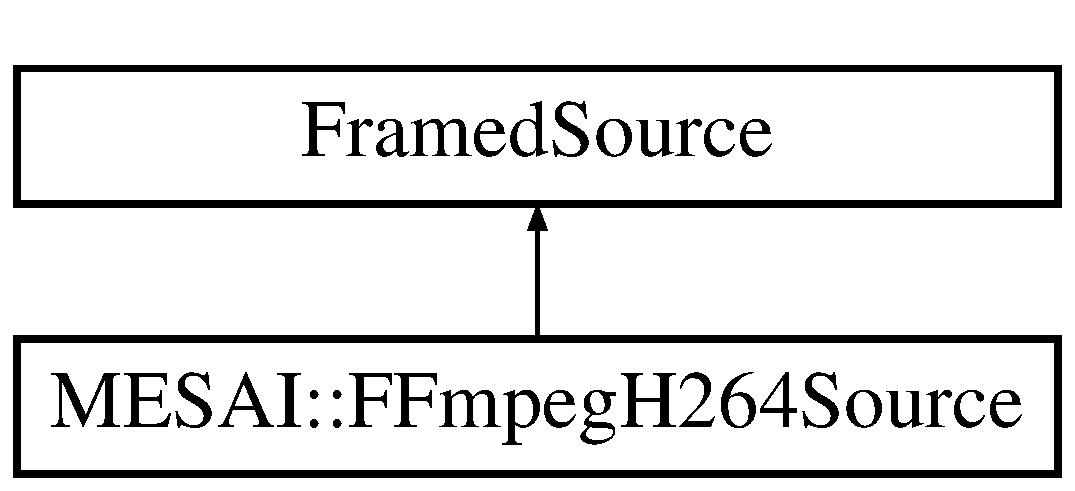
\includegraphics[height=2.000000cm]{d5/d44/class_m_e_s_a_i_1_1_f_fmpeg_h264_source}
\end{center}
\end{figure}
\subsection*{Public Member Functions}
\begin{DoxyCompactItemize}
\item 
\mbox{\Hypertarget{class_m_e_s_a_i_1_1_f_fmpeg_h264_source_a016ab12aa100999b35fd9a4d35fd17df}\label{class_m_e_s_a_i_1_1_f_fmpeg_h264_source_a016ab12aa100999b35fd9a4d35fd17df}} 
{\bfseries F\+Fmpeg\+H264\+Source} (Usage\+Environment \&env, \hyperlink{class_m_e_s_a_i_1_1_f_fmpeg_h264_encoder}{F\+Fmpeg\+H264\+Encoder} $\ast$E\+\_\+\+Source)
\end{DoxyCompactItemize}
\subsection*{Static Public Member Functions}
\begin{DoxyCompactItemize}
\item 
\mbox{\Hypertarget{class_m_e_s_a_i_1_1_f_fmpeg_h264_source_a7f9f2e3889579dac315e0ede519e1c12}\label{class_m_e_s_a_i_1_1_f_fmpeg_h264_source_a7f9f2e3889579dac315e0ede519e1c12}} 
static \hyperlink{class_m_e_s_a_i_1_1_f_fmpeg_h264_source}{F\+Fmpeg\+H264\+Source} $\ast$ {\bfseries create\+New} (Usage\+Environment \&env, \hyperlink{class_m_e_s_a_i_1_1_f_fmpeg_h264_encoder}{F\+Fmpeg\+H264\+Encoder} $\ast$E\+\_\+\+Source)
\end{DoxyCompactItemize}
\subsection*{Private Member Functions}
\begin{DoxyCompactItemize}
\item 
\mbox{\Hypertarget{class_m_e_s_a_i_1_1_f_fmpeg_h264_source_a967007b841277947e271d1012e7c7c95}\label{class_m_e_s_a_i_1_1_f_fmpeg_h264_source_a967007b841277947e271d1012e7c7c95}} 
virtual void {\bfseries do\+Get\+Next\+Frame} ()
\item 
\mbox{\Hypertarget{class_m_e_s_a_i_1_1_f_fmpeg_h264_source_a622a01cbb91ef6c7d61bf3c74ddead35}\label{class_m_e_s_a_i_1_1_f_fmpeg_h264_source_a622a01cbb91ef6c7d61bf3c74ddead35}} 
void {\bfseries deliver\+Frame} ()
\item 
\mbox{\Hypertarget{class_m_e_s_a_i_1_1_f_fmpeg_h264_source_a1a10200e6ac4565e6460438190162a69}\label{class_m_e_s_a_i_1_1_f_fmpeg_h264_source_a1a10200e6ac4565e6460438190162a69}} 
virtual void {\bfseries do\+Stop\+Getting\+Frames} ()
\item 
\mbox{\Hypertarget{class_m_e_s_a_i_1_1_f_fmpeg_h264_source_ad7f4d5cd5f7c11b745d0cd4368ef157b}\label{class_m_e_s_a_i_1_1_f_fmpeg_h264_source_ad7f4d5cd5f7c11b745d0cd4368ef157b}} 
void {\bfseries on\+Frame} ()
\end{DoxyCompactItemize}
\subsection*{Static Private Member Functions}
\begin{DoxyCompactItemize}
\item 
\mbox{\Hypertarget{class_m_e_s_a_i_1_1_f_fmpeg_h264_source_ab41b999be77633742ad0ea561dfad290}\label{class_m_e_s_a_i_1_1_f_fmpeg_h264_source_ab41b999be77633742ad0ea561dfad290}} 
static void {\bfseries deliver\+Frame\+Stub} (void $\ast$client\+Data)
\end{DoxyCompactItemize}
\subsection*{Private Attributes}
\begin{DoxyCompactItemize}
\item 
\mbox{\Hypertarget{class_m_e_s_a_i_1_1_f_fmpeg_h264_source_ab1f1e923491eb519f4963b2207252939}\label{class_m_e_s_a_i_1_1_f_fmpeg_h264_source_ab1f1e923491eb519f4963b2207252939}} 
\hyperlink{class_m_e_s_a_i_1_1_f_fmpeg_h264_encoder}{F\+Fmpeg\+H264\+Encoder} $\ast$ {\bfseries Encoding\+\_\+\+Source}
\item 
\mbox{\Hypertarget{class_m_e_s_a_i_1_1_f_fmpeg_h264_source_a9a6f3a78d3c5c8040e64b7192bcd424f}\label{class_m_e_s_a_i_1_1_f_fmpeg_h264_source_a9a6f3a78d3c5c8040e64b7192bcd424f}} 
Event\+Trigger\+Id {\bfseries m\+\_\+event\+Trigger\+Id}
\end{DoxyCompactItemize}


The documentation for this class was generated from the following files\+:\begin{DoxyCompactItemize}
\item 
header/streaming\+\_\+rtsp/F\+Fmpeg\+H264\+Source.\+h\item 
source/streaming\+\_\+rtsp/F\+Fmpeg\+H264\+Source.\+cpp\end{DoxyCompactItemize}

\hypertarget{class_f_fmpeg_opencv_decoder}{}\section{F\+Fmpeg\+Opencv\+Decoder Class Reference}
\label{class_f_fmpeg_opencv_decoder}\index{F\+Fmpeg\+Opencv\+Decoder@{F\+Fmpeg\+Opencv\+Decoder}}
Inheritance diagram for F\+Fmpeg\+Opencv\+Decoder\+:\begin{figure}[H]
\begin{center}
\leavevmode
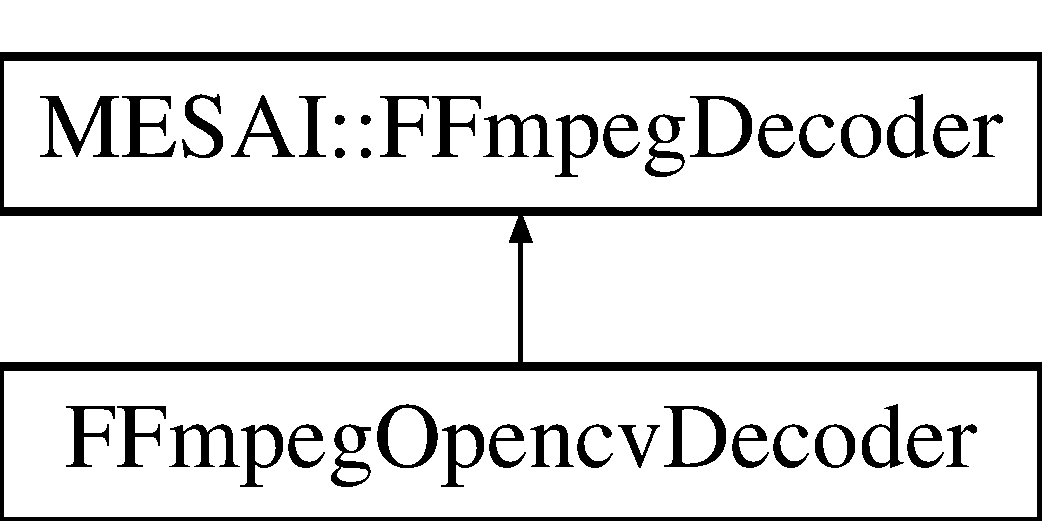
\includegraphics[height=2.000000cm]{d4/da2/class_f_fmpeg_opencv_decoder}
\end{center}
\end{figure}
\subsection*{Classes}
\begin{DoxyCompactItemize}
\item 
struct \hyperlink{struct_f_fmpeg_opencv_decoder_1_1config}{config}
\end{DoxyCompactItemize}
\subsection*{Public Member Functions}
\begin{DoxyCompactItemize}
\item 
\mbox{\Hypertarget{class_f_fmpeg_opencv_decoder_a420523542393ea9308a8eeec8b14ba71}\label{class_f_fmpeg_opencv_decoder_a420523542393ea9308a8eeec8b14ba71}} 
{\bfseries F\+Fmpeg\+Opencv\+Decoder} (\hyperlink{struct_f_fmpeg_opencv_decoder_1_1config}{F\+Fmpeg\+Opencv\+Decoder\+::config} conf)
\item 
\mbox{\Hypertarget{class_f_fmpeg_opencv_decoder_aac56e6cba67cb1808d0acf390aa1facc}\label{class_f_fmpeg_opencv_decoder_aac56e6cba67cb1808d0acf390aa1facc}} 
virtual void {\bfseries intialize} ()
\item 
\mbox{\Hypertarget{class_f_fmpeg_opencv_decoder_ab63e4419664779b1b213a972193aca10}\label{class_f_fmpeg_opencv_decoder_ab63e4419664779b1b213a972193aca10}} 
virtual void {\bfseries play\+Media} ()
\end{DoxyCompactItemize}
\subsection*{Public Attributes}
\begin{DoxyCompactItemize}
\item 
\mbox{\Hypertarget{class_f_fmpeg_opencv_decoder_ab55a686c783ddc11c410e03c44afad2e}\label{class_f_fmpeg_opencv_decoder_ab55a686c783ddc11c410e03c44afad2e}} 
\hyperlink{struct_f_fmpeg_opencv_decoder_1_1config}{F\+Fmpeg\+Opencv\+Decoder\+::config} {\bfseries \+\_\+conf}
\item 
\mbox{\Hypertarget{class_f_fmpeg_opencv_decoder_a88088faff211836083da0014ae3baeb9}\label{class_f_fmpeg_opencv_decoder_a88088faff211836083da0014ae3baeb9}} 
cv\+::\+Video\+Capture {\bfseries video}
\end{DoxyCompactItemize}
\subsection*{Additional Inherited Members}


The documentation for this class was generated from the following files\+:\begin{DoxyCompactItemize}
\item 
header/streaming\+\_\+rtsp/F\+Fmpeg\+Opencv\+Decoder.\+h\item 
source/streaming\+\_\+rtsp/F\+Fmpeg\+Opencv\+Decoder.\+cpp\end{DoxyCompactItemize}

\hypertarget{classfilter_1_1data_1_1_file_image_data}{}\section{filter\+:\+:data\+:\+:File\+Image\+Data Class Reference}
\label{classfilter_1_1data_1_1_file_image_data}\index{filter\+::data\+::\+File\+Image\+Data@{filter\+::data\+::\+File\+Image\+Data}}


\hyperlink{classfilter_1_1data_1_1_file_image_data}{File\+Image\+Data} is the data type used to handle an image and additonnal information. Uses Open\+CV.  




{\ttfamily \#include $<$File\+Image\+Data.\+h$>$}

Inheritance diagram for filter\+:\+:data\+:\+:File\+Image\+Data\+:\begin{figure}[H]
\begin{center}
\leavevmode
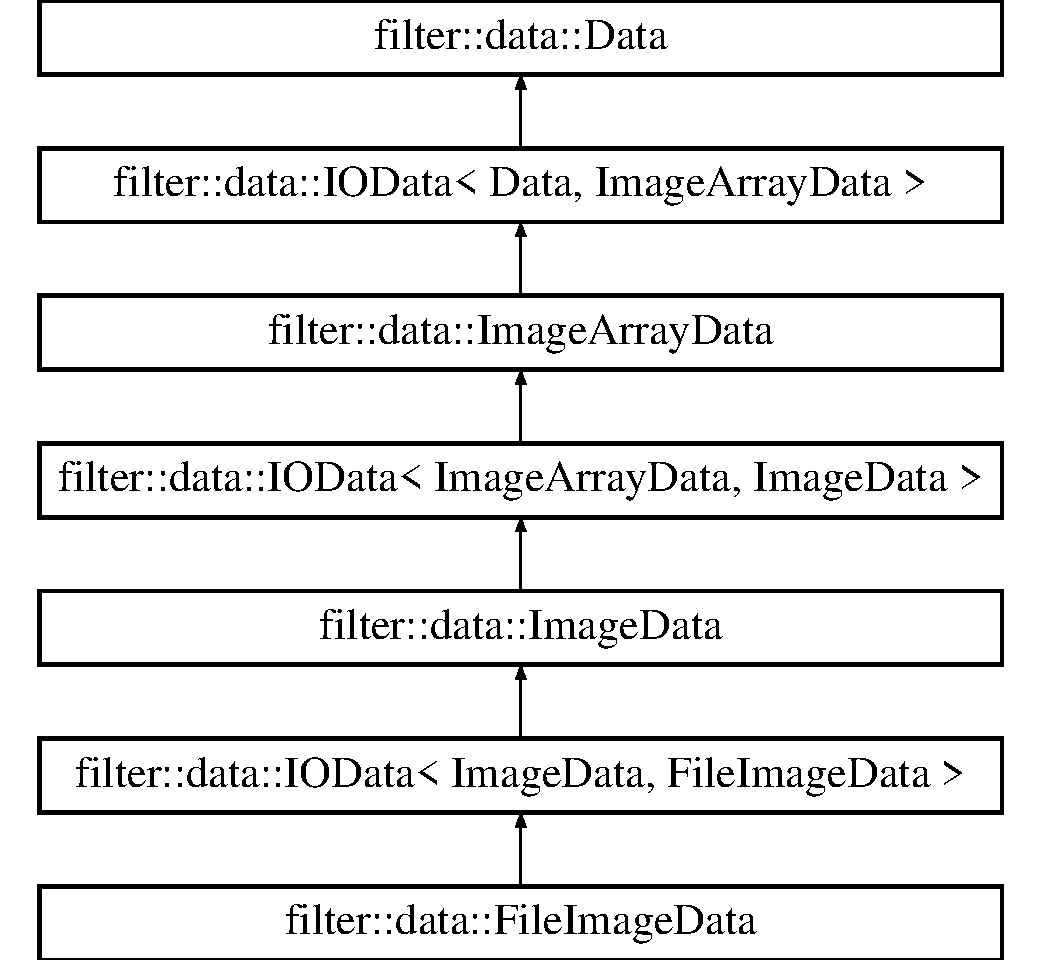
\includegraphics[height=7.000000cm]{d7/dc4/classfilter_1_1data_1_1_file_image_data}
\end{center}
\end{figure}
\subsection*{Public Member Functions}
\begin{DoxyCompactItemize}
\item 
\hyperlink{classfilter_1_1data_1_1_file_image_data_aa49f9012959f0f8f8c1826be3a31fdf6}{File\+Image\+Data} (const \hyperlink{classfilter_1_1data_1_1_file_image_data}{File\+Image\+Data} \&right)
\begin{DoxyCompactList}\small\item\em \hyperlink{classfilter_1_1data_1_1_file_image_data}{File\+Image\+Data} copy constructor. \end{DoxyCompactList}\item 
\hyperlink{classfilter_1_1data_1_1_file_image_data_ad5fb185db36ade62bc5eb46d30b938a1}{File\+Image\+Data} (const std\+::string \&file\+Path)
\begin{DoxyCompactList}\small\item\em Constructor with path to image. \end{DoxyCompactList}\item 
virtual void \hyperlink{classfilter_1_1data_1_1_file_image_data_a188f2f5ab66877f6ba553cc847cd5f07}{copy\+To} (\hyperlink{classfilter_1_1data_1_1_image_data}{Image\+Data} \&left) const
\begin{DoxyCompactList}\small\item\em Copy the image data of the \hyperlink{classfilter_1_1data_1_1_image_data}{Image\+Data} object to another one. \end{DoxyCompactList}\item 
\hyperlink{classfilter_1_1data_1_1_file_image_data}{File\+Image\+Data} \& \hyperlink{classfilter_1_1data_1_1_file_image_data_abd280bc0cc3d1a1e6aa1924041a71820}{operator=} (const \hyperlink{classfilter_1_1data_1_1_file_image_data}{File\+Image\+Data} \&left)
\begin{DoxyCompactList}\small\item\em \hyperlink{classfilter_1_1data_1_1_file_image_data}{File\+Image\+Data} assignment operator. \end{DoxyCompactList}\end{DoxyCompactItemize}
\subsection*{Private Member Functions}
\begin{DoxyCompactItemize}
\item 
\mbox{\Hypertarget{classfilter_1_1data_1_1_file_image_data_aef2ffb7b62f14ba6312bbb21167b13f3}\label{classfilter_1_1data_1_1_file_image_data_aef2ffb7b62f14ba6312bbb21167b13f3}} 
cv\+::\+Mat {\bfseries as\+Output} ()
\end{DoxyCompactItemize}
\subsection*{Private Attributes}
\begin{DoxyCompactItemize}
\item 
\mbox{\Hypertarget{classfilter_1_1data_1_1_file_image_data_ac40a6678009c5f0745adc81ff32ea2ef}\label{classfilter_1_1data_1_1_file_image_data_ac40a6678009c5f0745adc81ff32ea2ef}} 
boost\+::filesystem\+::path \hyperlink{classfilter_1_1data_1_1_file_image_data_ac40a6678009c5f0745adc81ff32ea2ef}{\+\_\+file\+Path}
\begin{DoxyCompactList}\small\item\em Path to the image. \end{DoxyCompactList}\end{DoxyCompactItemize}
\subsection*{Additional Inherited Members}


\subsection{Constructor \& Destructor Documentation}
\mbox{\Hypertarget{classfilter_1_1data_1_1_file_image_data_aa49f9012959f0f8f8c1826be3a31fdf6}\label{classfilter_1_1data_1_1_file_image_data_aa49f9012959f0f8f8c1826be3a31fdf6}} 
\index{filter\+::data\+::\+File\+Image\+Data@{filter\+::data\+::\+File\+Image\+Data}!File\+Image\+Data@{File\+Image\+Data}}
\index{File\+Image\+Data@{File\+Image\+Data}!filter\+::data\+::\+File\+Image\+Data@{filter\+::data\+::\+File\+Image\+Data}}
\subsubsection{\texorpdfstring{File\+Image\+Data()}{FileImageData()}\hspace{0.1cm}{\footnotesize\ttfamily [1/2]}}
{\footnotesize\ttfamily filter\+::data\+::\+File\+Image\+Data\+::\+File\+Image\+Data (\begin{DoxyParamCaption}\item[{const \hyperlink{classfilter_1_1data_1_1_file_image_data}{File\+Image\+Data} \&}]{right }\end{DoxyParamCaption})\hspace{0.3cm}{\ttfamily [inline]}}


\begin{DoxyParams}{Parameters}
{\em right} & the \hyperlink{classfilter_1_1data_1_1_file_image_data}{File\+Image\+Data} to copy \\
\hline
\end{DoxyParams}
\mbox{\Hypertarget{classfilter_1_1data_1_1_file_image_data_ad5fb185db36ade62bc5eb46d30b938a1}\label{classfilter_1_1data_1_1_file_image_data_ad5fb185db36ade62bc5eb46d30b938a1}} 
\index{filter\+::data\+::\+File\+Image\+Data@{filter\+::data\+::\+File\+Image\+Data}!File\+Image\+Data@{File\+Image\+Data}}
\index{File\+Image\+Data@{File\+Image\+Data}!filter\+::data\+::\+File\+Image\+Data@{filter\+::data\+::\+File\+Image\+Data}}
\subsubsection{\texorpdfstring{File\+Image\+Data()}{FileImageData()}\hspace{0.1cm}{\footnotesize\ttfamily [2/2]}}
{\footnotesize\ttfamily filter\+::data\+::\+File\+Image\+Data\+::\+File\+Image\+Data (\begin{DoxyParamCaption}\item[{const std\+::string \&}]{file\+Path }\end{DoxyParamCaption})\hspace{0.3cm}{\ttfamily [inline]}}


\begin{DoxyParams}{Parameters}
{\em file\+Path} & Complete path to the image \\
\hline
\end{DoxyParams}


\subsection{Member Function Documentation}
\mbox{\Hypertarget{classfilter_1_1data_1_1_file_image_data_a188f2f5ab66877f6ba553cc847cd5f07}\label{classfilter_1_1data_1_1_file_image_data_a188f2f5ab66877f6ba553cc847cd5f07}} 
\index{filter\+::data\+::\+File\+Image\+Data@{filter\+::data\+::\+File\+Image\+Data}!copy\+To@{copy\+To}}
\index{copy\+To@{copy\+To}!filter\+::data\+::\+File\+Image\+Data@{filter\+::data\+::\+File\+Image\+Data}}
\subsubsection{\texorpdfstring{copy\+To()}{copyTo()}}
{\footnotesize\ttfamily virtual void filter\+::data\+::\+File\+Image\+Data\+::copy\+To (\begin{DoxyParamCaption}\item[{\hyperlink{classfilter_1_1data_1_1_image_data}{Image\+Data} \&}]{left }\end{DoxyParamCaption}) const\hspace{0.3cm}{\ttfamily [inline]}, {\ttfamily [virtual]}}


\begin{DoxyParams}{Parameters}
{\em left} & The object where to copy the data to \\
\hline
\end{DoxyParams}


Reimplemented from \hyperlink{classfilter_1_1data_1_1_image_data_ab035bfe80f8f6a6470046eb15fad7dfb}{filter\+::data\+::\+Image\+Data}.

\mbox{\Hypertarget{classfilter_1_1data_1_1_file_image_data_abd280bc0cc3d1a1e6aa1924041a71820}\label{classfilter_1_1data_1_1_file_image_data_abd280bc0cc3d1a1e6aa1924041a71820}} 
\index{filter\+::data\+::\+File\+Image\+Data@{filter\+::data\+::\+File\+Image\+Data}!operator=@{operator=}}
\index{operator=@{operator=}!filter\+::data\+::\+File\+Image\+Data@{filter\+::data\+::\+File\+Image\+Data}}
\subsubsection{\texorpdfstring{operator=()}{operator=()}}
{\footnotesize\ttfamily \hyperlink{classfilter_1_1data_1_1_file_image_data}{File\+Image\+Data}\& filter\+::data\+::\+File\+Image\+Data\+::operator= (\begin{DoxyParamCaption}\item[{const \hyperlink{classfilter_1_1data_1_1_file_image_data}{File\+Image\+Data} \&}]{left }\end{DoxyParamCaption})\hspace{0.3cm}{\ttfamily [inline]}}

\begin{DoxyRefDesc}{Todo}
\item[\hyperlink{todo__todo000020}{Todo}]\end{DoxyRefDesc}

\begin{DoxyParams}{Parameters}
{\em left} & The \hyperlink{classfilter_1_1data_1_1_file_image_data}{File\+Image\+Data} object to get the data from \\
\hline
\end{DoxyParams}
\begin{DoxyReturn}{Returns}
A reference to the object 
\end{DoxyReturn}


The documentation for this class was generated from the following file\+:\begin{DoxyCompactItemize}
\item 
header/filter/data/File\+Image\+Data.\+h\end{DoxyCompactItemize}

\hypertarget{classfilter_1_1data_1_1_file_video_input}{}\section{filter\+:\+:data\+:\+:File\+Video\+Input Class Reference}
\label{classfilter_1_1data_1_1_file_video_input}\index{filter\+::data\+::\+File\+Video\+Input@{filter\+::data\+::\+File\+Video\+Input}}


\hyperlink{classfilter_1_1data_1_1_file_video_input}{File\+Video\+Input} is the data type used to handle a video. Uses Open\+CV.  




{\ttfamily \#include $<$File\+Video\+Input.\+h$>$}

Inheritance diagram for filter\+:\+:data\+:\+:File\+Video\+Input\+:\begin{figure}[H]
\begin{center}
\leavevmode
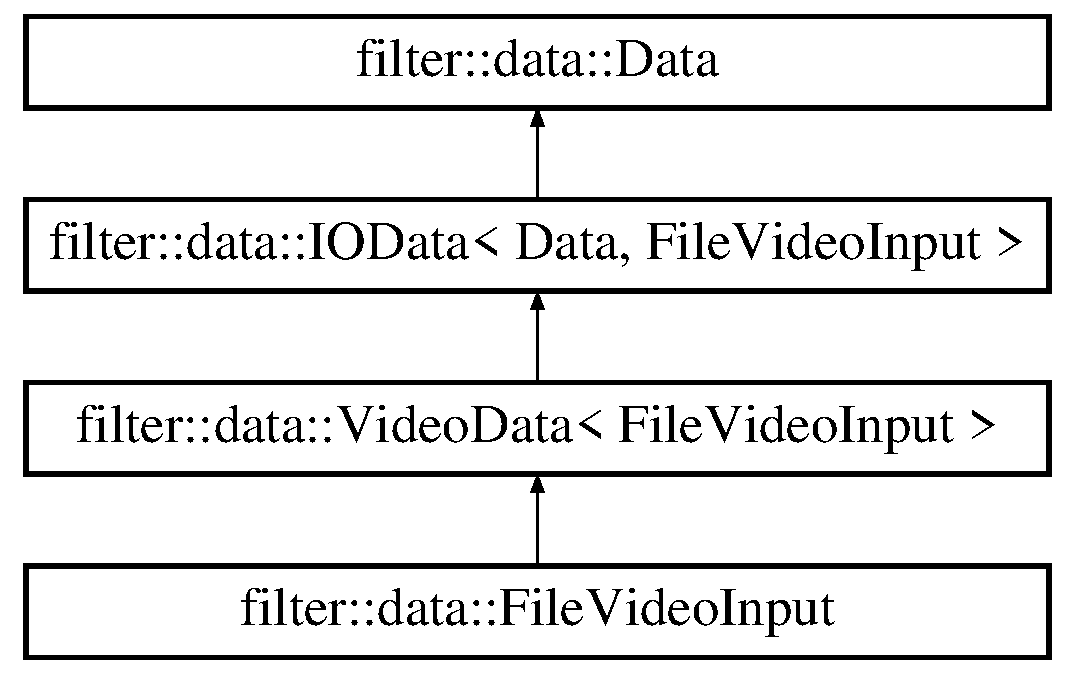
\includegraphics[height=4.000000cm]{dd/da2/classfilter_1_1data_1_1_file_video_input}
\end{center}
\end{figure}
\subsection*{Public Member Functions}
\begin{DoxyCompactItemize}
\item 
\hyperlink{classfilter_1_1data_1_1_file_video_input_aa585659183e8225ad97fafffe5e58dca}{File\+Video\+Input} (const std\+::string \&file\+Path, bool loop)
\item 
\mbox{\Hypertarget{classfilter_1_1data_1_1_file_video_input_a569f7c6c2258bfd5d341454e0d1e09dc}\label{classfilter_1_1data_1_1_file_video_input_a569f7c6c2258bfd5d341454e0d1e09dc}} 
{\bfseries File\+Video\+Input} (const \hyperlink{classfilter_1_1data_1_1_file_video_input}{File\+Video\+Input} \&data)
\item 
\mbox{\Hypertarget{classfilter_1_1data_1_1_file_video_input_aa564a2cee2252263afdbd61dfdab709f}\label{classfilter_1_1data_1_1_file_video_input_aa564a2cee2252263afdbd61dfdab709f}} 
void \hyperlink{classfilter_1_1data_1_1_file_video_input_aa564a2cee2252263afdbd61dfdab709f}{open\+File} ()
\begin{DoxyCompactList}\small\item\em Opens a video file from its path, if valid. \end{DoxyCompactList}\item 
\hyperlink{classfilter_1_1data_1_1_data}{Data} \hyperlink{classfilter_1_1data_1_1_file_video_input_a01a93b368b1a8192c47490ff554ad30f}{new\+Frame} ()
\begin{DoxyCompactList}\small\item\em Get the next frame of the video. \end{DoxyCompactList}\item 
bool \hyperlink{classfilter_1_1data_1_1_file_video_input_a7db00de01c31e63d49a518e737ab8799}{empty} () const
\begin{DoxyCompactList}\small\item\em Checks if the File\+Video is empty. \end{DoxyCompactList}\end{DoxyCompactItemize}
\subsection*{Private Member Functions}
\begin{DoxyCompactItemize}
\item 
\mbox{\Hypertarget{classfilter_1_1data_1_1_file_video_input_a1795703ad8ea105b857534a32e14f295}\label{classfilter_1_1data_1_1_file_video_input_a1795703ad8ea105b857534a32e14f295}} 
cv\+::\+Mat {\bfseries as\+Output} ()
\end{DoxyCompactItemize}
\subsection*{Private Attributes}
\begin{DoxyCompactItemize}
\item 
\mbox{\Hypertarget{classfilter_1_1data_1_1_file_video_input_a3688b3fe35d4e53bb77340c937c837e1}\label{classfilter_1_1data_1_1_file_video_input_a3688b3fe35d4e53bb77340c937c837e1}} 
boost\+::filesystem\+::path \hyperlink{classfilter_1_1data_1_1_file_video_input_a3688b3fe35d4e53bb77340c937c837e1}{\+\_\+file\+Path}
\begin{DoxyCompactList}\small\item\em Path of the video. \end{DoxyCompactList}\item 
\mbox{\Hypertarget{classfilter_1_1data_1_1_file_video_input_af9be93f58c33b095c635ca43fbeedc64}\label{classfilter_1_1data_1_1_file_video_input_af9be93f58c33b095c635ca43fbeedc64}} 
cv\+::\+Video\+Capture \hyperlink{classfilter_1_1data_1_1_file_video_input_af9be93f58c33b095c635ca43fbeedc64}{\+\_\+capture}
\begin{DoxyCompactList}\small\item\em Handles the reading of the video\textquotesingle{}s frames. \end{DoxyCompactList}\item 
\mbox{\Hypertarget{classfilter_1_1data_1_1_file_video_input_a845591eabd4f19be613d0f5284baf38f}\label{classfilter_1_1data_1_1_file_video_input_a845591eabd4f19be613d0f5284baf38f}} 
bool \hyperlink{classfilter_1_1data_1_1_file_video_input_a845591eabd4f19be613d0f5284baf38f}{\+\_\+loop}
\begin{DoxyCompactList}\small\item\em If set to true, loops the video at the end of the playback. \end{DoxyCompactList}\end{DoxyCompactItemize}
\subsection*{Additional Inherited Members}


\subsection{Constructor \& Destructor Documentation}
\mbox{\Hypertarget{classfilter_1_1data_1_1_file_video_input_aa585659183e8225ad97fafffe5e58dca}\label{classfilter_1_1data_1_1_file_video_input_aa585659183e8225ad97fafffe5e58dca}} 
\index{filter\+::data\+::\+File\+Video\+Input@{filter\+::data\+::\+File\+Video\+Input}!File\+Video\+Input@{File\+Video\+Input}}
\index{File\+Video\+Input@{File\+Video\+Input}!filter\+::data\+::\+File\+Video\+Input@{filter\+::data\+::\+File\+Video\+Input}}
\subsubsection{\texorpdfstring{File\+Video\+Input()}{FileVideoInput()}}
{\footnotesize\ttfamily filter\+::data\+::\+File\+Video\+Input\+::\+File\+Video\+Input (\begin{DoxyParamCaption}\item[{const std\+::string \&}]{file\+Path,  }\item[{bool}]{loop }\end{DoxyParamCaption})\hspace{0.3cm}{\ttfamily [inline]}}


\begin{DoxyParams}{Parameters}
{\em file\+Path} & the path to the video file \\
\hline
{\em loop} & Should the video loop on playback end \\
\hline
\end{DoxyParams}


\subsection{Member Function Documentation}
\mbox{\Hypertarget{classfilter_1_1data_1_1_file_video_input_a7db00de01c31e63d49a518e737ab8799}\label{classfilter_1_1data_1_1_file_video_input_a7db00de01c31e63d49a518e737ab8799}} 
\index{filter\+::data\+::\+File\+Video\+Input@{filter\+::data\+::\+File\+Video\+Input}!empty@{empty}}
\index{empty@{empty}!filter\+::data\+::\+File\+Video\+Input@{filter\+::data\+::\+File\+Video\+Input}}
\subsubsection{\texorpdfstring{empty()}{empty()}}
{\footnotesize\ttfamily bool filter\+::data\+::\+File\+Video\+Input\+::empty (\begin{DoxyParamCaption}{ }\end{DoxyParamCaption}) const\hspace{0.3cm}{\ttfamily [inline]}, {\ttfamily [virtual]}}

\begin{DoxyRefDesc}{Todo}
\item[\hyperlink{todo__todo000021}{Todo}]\end{DoxyRefDesc}
\begin{DoxyReturn}{Returns}
Returns true if the object doesn\textquotesingle{}t contain any data or the video is not opened, false either. 
\end{DoxyReturn}


Reimplemented from \hyperlink{classfilter_1_1data_1_1_i_o_data}{filter\+::data\+::\+I\+O\+Data$<$ Data, File\+Video\+Input $>$}.

\mbox{\Hypertarget{classfilter_1_1data_1_1_file_video_input_a01a93b368b1a8192c47490ff554ad30f}\label{classfilter_1_1data_1_1_file_video_input_a01a93b368b1a8192c47490ff554ad30f}} 
\index{filter\+::data\+::\+File\+Video\+Input@{filter\+::data\+::\+File\+Video\+Input}!new\+Frame@{new\+Frame}}
\index{new\+Frame@{new\+Frame}!filter\+::data\+::\+File\+Video\+Input@{filter\+::data\+::\+File\+Video\+Input}}
\subsubsection{\texorpdfstring{new\+Frame()}{newFrame()}}
{\footnotesize\ttfamily \hyperlink{classfilter_1_1data_1_1_data}{Data} filter\+::data\+::\+File\+Video\+Input\+::new\+Frame (\begin{DoxyParamCaption}{ }\end{DoxyParamCaption})\hspace{0.3cm}{\ttfamily [inline]}}

\begin{DoxyReturn}{Returns}
Return the next frame of the video as a 
\end{DoxyReturn}
\begin{DoxySeeAlso}{See also}
\hyperlink{classfilter_1_1data_1_1_data}{Data} object, or a black one if the plaback already ended and the loop option is disabled 
\end{DoxySeeAlso}


The documentation for this class was generated from the following file\+:\begin{DoxyCompactItemize}
\item 
header/filter/data/File\+Video\+Input.\+h\end{DoxyCompactItemize}

\hypertarget{class_m_e_s_a_i_1_1_frame_structure}{}\section{M\+E\+S\+AI\+:\+:Frame\+Structure Class Reference}
\label{class_m_e_s_a_i_1_1_frame_structure}\index{M\+E\+S\+A\+I\+::\+Frame\+Structure@{M\+E\+S\+A\+I\+::\+Frame\+Structure}}
\subsection*{Public Attributes}
\begin{DoxyCompactItemize}
\item 
\mbox{\Hypertarget{class_m_e_s_a_i_1_1_frame_structure_a69fdf446d3c9212c62ecf845414a6391}\label{class_m_e_s_a_i_1_1_frame_structure_a69fdf446d3c9212c62ecf845414a6391}} 
uint8\+\_\+t $\ast$ {\bfseries data\+Pointer}
\item 
\mbox{\Hypertarget{class_m_e_s_a_i_1_1_frame_structure_ad5e93a14647887d6e5cba08bbde462ab}\label{class_m_e_s_a_i_1_1_frame_structure_ad5e93a14647887d6e5cba08bbde462ab}} 
int {\bfseries data\+Size}
\item 
\mbox{\Hypertarget{class_m_e_s_a_i_1_1_frame_structure_ac2de50e7925e198c85597b593be5338a}\label{class_m_e_s_a_i_1_1_frame_structure_ac2de50e7925e198c85597b593be5338a}} 
int {\bfseries frame\+ID}
\end{DoxyCompactItemize}


The documentation for this class was generated from the following file\+:\begin{DoxyCompactItemize}
\item 
header/streaming\+\_\+rtsp/F\+Fmpeg\+H264\+Encoder.\+h\end{DoxyCompactItemize}

\hypertarget{structhttp_1_1_command_manager_1_1function__traits}{}\section{http\+:\+:Command\+Manager\+:\+:function\+\_\+traits$<$ T $>$ Struct Template Reference}
\label{structhttp_1_1_command_manager_1_1function__traits}\index{http\+::\+Command\+Manager\+::function\+\_\+traits$<$ T $>$@{http\+::\+Command\+Manager\+::function\+\_\+traits$<$ T $>$}}


The documentation for this struct was generated from the following file\+:\begin{DoxyCompactItemize}
\item 
header/http/Command\+Manager.\+h\end{DoxyCompactItemize}

\hypertarget{structhttp_1_1_command_manager_1_1function__traits_3_01_return_type_07_5_08_07_args_01_8_8_8_08_4}{}\section{http\+:\+:Command\+Manager\+:\+:function\+\_\+traits$<$ Return\+Type($\ast$)(Args ...)$>$ Struct Template Reference}
\label{structhttp_1_1_command_manager_1_1function__traits_3_01_return_type_07_5_08_07_args_01_8_8_8_08_4}\index{http\+::\+Command\+Manager\+::function\+\_\+traits$<$ Return\+Type($\ast$)(\+Args ...)$>$@{http\+::\+Command\+Manager\+::function\+\_\+traits$<$ Return\+Type($\ast$)(\+Args ...)$>$}}
\subsection*{Public Types}
\begin{DoxyCompactItemize}
\item 
\mbox{\Hypertarget{structhttp_1_1_command_manager_1_1function__traits_3_01_return_type_07_5_08_07_args_01_8_8_8_08_4_a88388662cb4f77f652df2fe76937146d}\label{structhttp_1_1_command_manager_1_1function__traits_3_01_return_type_07_5_08_07_args_01_8_8_8_08_4_a88388662cb4f77f652df2fe76937146d}} 
typedef std\+::function$<$ Return\+Type(Args ...)$>$ {\bfseries f\+\_\+type}
\end{DoxyCompactItemize}


The documentation for this struct was generated from the following file\+:\begin{DoxyCompactItemize}
\item 
header/http/Command\+Manager.\+h\end{DoxyCompactItemize}

\hypertarget{structhttp_1_1_command_manager_1_1function__traits_3_01_return_type_07_class_type_1_1_5_08_07_args_01_8_8_8_08_01const_01_4}{}\section{http\+:\+:Command\+Manager\+:\+:function\+\_\+traits$<$ Return\+Type(Class\+Type\+:\+:$\ast$)(Args ...) const $>$ Struct Template Reference}
\label{structhttp_1_1_command_manager_1_1function__traits_3_01_return_type_07_class_type_1_1_5_08_07_args_01_8_8_8_08_01const_01_4}\index{http\+::\+Command\+Manager\+::function\+\_\+traits$<$ Return\+Type(\+Class\+Type\+::$\ast$)(\+Args ...) const $>$@{http\+::\+Command\+Manager\+::function\+\_\+traits$<$ Return\+Type(\+Class\+Type\+::$\ast$)(\+Args ...) const $>$}}
\subsection*{Public Types}
\begin{DoxyCompactItemize}
\item 
\mbox{\Hypertarget{structhttp_1_1_command_manager_1_1function__traits_3_01_return_type_07_class_type_1_1_5_08_07_args_01_8_8_8_08_01const_01_4_af755381d54336a7a35d381dfa2137796}\label{structhttp_1_1_command_manager_1_1function__traits_3_01_return_type_07_class_type_1_1_5_08_07_args_01_8_8_8_08_01const_01_4_af755381d54336a7a35d381dfa2137796}} 
typedef std\+::function$<$ Return\+Type(Args ...)$>$ {\bfseries f\+\_\+type}
\end{DoxyCompactItemize}


The documentation for this struct was generated from the following file\+:\begin{DoxyCompactItemize}
\item 
header/http/Command\+Manager.\+h\end{DoxyCompactItemize}

\hypertarget{structhttp_1_1_command_manager_1_1function__traits_3_01_return_type_07_class_type_1_1_5_08_07_args_01_8_8_8_08_4}{}\section{http\+:\+:Command\+Manager\+:\+:function\+\_\+traits$<$ Return\+Type(Class\+Type\+:\+:$\ast$)(Args ...)$>$ Struct Template Reference}
\label{structhttp_1_1_command_manager_1_1function__traits_3_01_return_type_07_class_type_1_1_5_08_07_args_01_8_8_8_08_4}\index{http\+::\+Command\+Manager\+::function\+\_\+traits$<$ Return\+Type(\+Class\+Type\+::$\ast$)(\+Args ...)$>$@{http\+::\+Command\+Manager\+::function\+\_\+traits$<$ Return\+Type(\+Class\+Type\+::$\ast$)(\+Args ...)$>$}}
\subsection*{Public Types}
\begin{DoxyCompactItemize}
\item 
\mbox{\Hypertarget{structhttp_1_1_command_manager_1_1function__traits_3_01_return_type_07_class_type_1_1_5_08_07_args_01_8_8_8_08_4_a3dc2482901f243f2dc4ec3ad3f89e3f8}\label{structhttp_1_1_command_manager_1_1function__traits_3_01_return_type_07_class_type_1_1_5_08_07_args_01_8_8_8_08_4_a3dc2482901f243f2dc4ec3ad3f89e3f8}} 
typedef std\+::function$<$ Return\+Type(Args ...)$>$ {\bfseries f\+\_\+type}
\end{DoxyCompactItemize}


The documentation for this struct was generated from the following file\+:\begin{DoxyCompactItemize}
\item 
header/http/Command\+Manager.\+h\end{DoxyCompactItemize}

\hypertarget{classfilter_1_1algos_1_1_gaussian}{}\section{filter\+:\+:algos\+:\+:Gaussian Class Reference}
\label{classfilter_1_1algos_1_1_gaussian}\index{filter\+::algos\+::\+Gaussian@{filter\+::algos\+::\+Gaussian}}
Inheritance diagram for filter\+:\+:algos\+:\+:Gaussian\+:\begin{figure}[H]
\begin{center}
\leavevmode
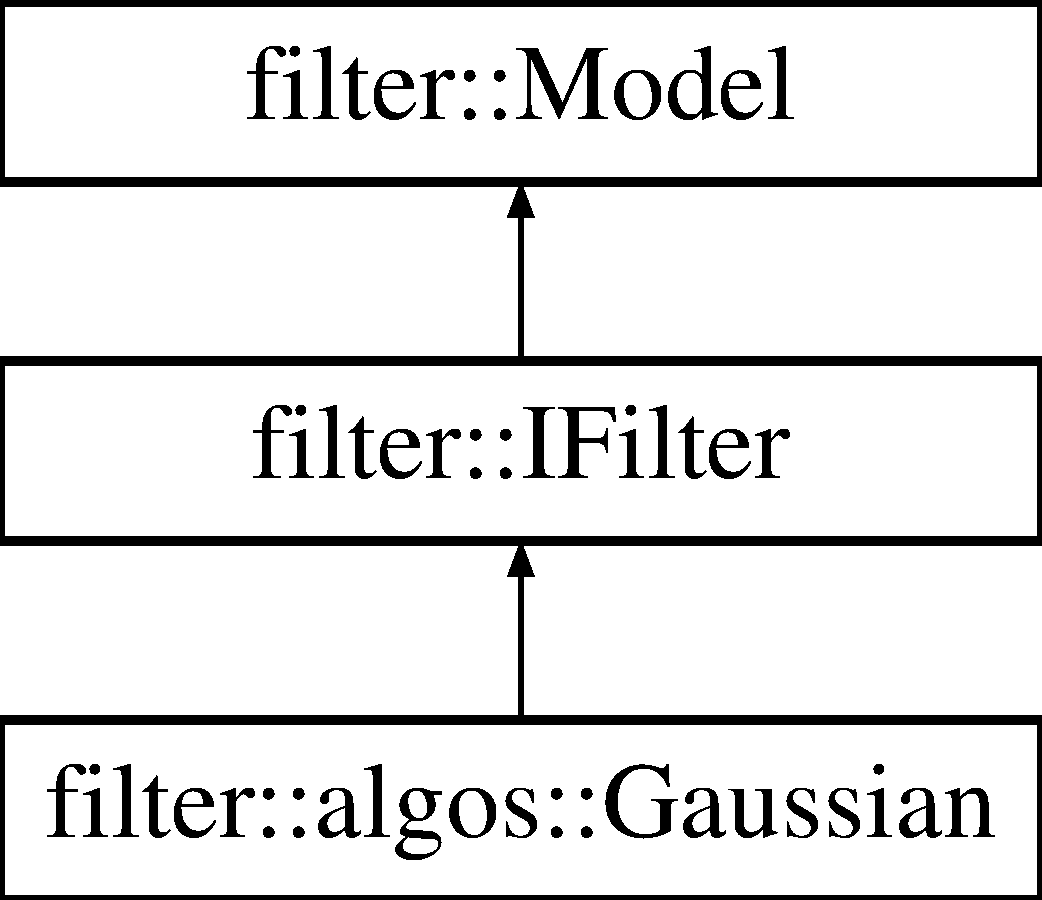
\includegraphics[height=3.000000cm]{db/d1c/classfilter_1_1algos_1_1_gaussian}
\end{center}
\end{figure}
\subsection*{Public Types}
\begin{DoxyCompactItemize}
\item 
\mbox{\Hypertarget{classfilter_1_1algos_1_1_gaussian_a2134cf203279385b1d54164997248342}\label{classfilter_1_1algos_1_1_gaussian_a2134cf203279385b1d54164997248342}} 
typedef \hyperlink{class_proxy_functor}{Proxy\+Functor}$<$ \hyperlink{classfilter_1_1algos_1_1_gaussian}{Gaussian} $>$ {\bfseries \+\_\+proxy\+Functor}
\item 
\mbox{\Hypertarget{classfilter_1_1algos_1_1_gaussian_ab9dd3d4c5f8e0c9e4955deacc2ce1108}\label{classfilter_1_1algos_1_1_gaussian_ab9dd3d4c5f8e0c9e4955deacc2ce1108}} 
typedef \hyperlink{classfilter_1_1algos_1_1_gaussian}{Gaussian} {\bfseries mytype}
\item 
\mbox{\Hypertarget{classfilter_1_1algos_1_1_gaussian_abfc9628637474ad4930c1a9a94f332c8}\label{classfilter_1_1algos_1_1_gaussian_abfc9628637474ad4930c1a9a94f332c8}} 
typedef int {\bfseries vartype\+\_\+\+\_\+sigma}
\end{DoxyCompactItemize}
\subsection*{Public Member Functions}
\begin{DoxyCompactItemize}
\item 
\mbox{\Hypertarget{classfilter_1_1algos_1_1_gaussian_ad6560679874af193ff2c27592c60dcd8}\label{classfilter_1_1algos_1_1_gaussian_ad6560679874af193ff2c27592c60dcd8}} 
void {\bfseries set\+\_\+sigma\+\_\+from\+\_\+json} (boost\+::property\+\_\+tree\+::ptree \&json\+Class)
\item 
\mbox{\Hypertarget{classfilter_1_1algos_1_1_gaussian_ab248437e17b0ba05f8a51797c3e15143}\label{classfilter_1_1algos_1_1_gaussian_ab248437e17b0ba05f8a51797c3e15143}} 
void {\bfseries set\+\_\+sigma} (vartype\+\_\+\+\_\+sigma \&\+\_\+\+\_\+sigma)
\item 
\mbox{\Hypertarget{classfilter_1_1algos_1_1_gaussian_a4e009d7489028c92cdf4a7c628fd6941}\label{classfilter_1_1algos_1_1_gaussian_a4e009d7489028c92cdf4a7c628fd6941}} 
vartype\+\_\+\+\_\+sigma {\bfseries get\+\_\+sigma} ()
\item 
\mbox{\Hypertarget{classfilter_1_1algos_1_1_gaussian_a8b888f2c9fe5ea129c4ffeff46097d24}\label{classfilter_1_1algos_1_1_gaussian_a8b888f2c9fe5ea129c4ffeff46097d24}} 
void {\bfseries copy\+\_\+sigma} (\hyperlink{classfilter_1_1algos_1_1_gaussian}{mytype} $\ast$instance)
\item 
virtual std\+::string \hyperlink{classfilter_1_1algos_1_1_gaussian_a5f2ba86fa61807781b46fe321e435c29}{result\+As\+String} ()
\begin{DoxyCompactList}\small\item\em Get the result of the processing done by the node. This method will return information only. The actual processing is done by the process() method. \end{DoxyCompactList}\item 
\mbox{\Hypertarget{classfilter_1_1algos_1_1_gaussian_ae7670cd03d12db1be0183ef0f37e1ba9}\label{classfilter_1_1algos_1_1_gaussian_ae7670cd03d12db1be0183ef0f37e1ba9}} 
Hipe\+Status {\bfseries process} ()
\end{DoxyCompactItemize}
\subsection*{Public Attributes}
\begin{DoxyCompactItemize}
\item 
\mbox{\Hypertarget{classfilter_1_1algos_1_1_gaussian_a79118061fdbbe44108324c68af3a389d}\label{classfilter_1_1algos_1_1_gaussian_a79118061fdbbe44108324c68af3a389d}} 
int {\bfseries sigma}
\end{DoxyCompactItemize}
\subsection*{Additional Inherited Members}


\subsection{Member Function Documentation}
\mbox{\Hypertarget{classfilter_1_1algos_1_1_gaussian_a5f2ba86fa61807781b46fe321e435c29}\label{classfilter_1_1algos_1_1_gaussian_a5f2ba86fa61807781b46fe321e435c29}} 
\index{filter\+::algos\+::\+Gaussian@{filter\+::algos\+::\+Gaussian}!result\+As\+String@{result\+As\+String}}
\index{result\+As\+String@{result\+As\+String}!filter\+::algos\+::\+Gaussian@{filter\+::algos\+::\+Gaussian}}
\subsubsection{\texorpdfstring{result\+As\+String()}{resultAsString()}}
{\footnotesize\ttfamily virtual std\+::string filter\+::algos\+::\+Gaussian\+::result\+As\+String (\begin{DoxyParamCaption}{ }\end{DoxyParamCaption})\hspace{0.3cm}{\ttfamily [inline]}, {\ttfamily [virtual]}}

\begin{DoxyReturn}{Returns}
A string containing the result of the processing done by the filter. 
\end{DoxyReturn}


Reimplemented from \hyperlink{classfilter_1_1_i_filter_ab99902b060a6d9edc3452a8c9f85e37e}{filter\+::\+I\+Filter}.



The documentation for this class was generated from the following file\+:\begin{DoxyCompactItemize}
\item 
header/filter/\+Algos/Gaussian.\+h\end{DoxyCompactItemize}

\hypertarget{classfilter_1_1algos_1_1_grayscale}{}\section{filter\+:\+:algos\+:\+:Grayscale Class Reference}
\label{classfilter_1_1algos_1_1_grayscale}\index{filter\+::algos\+::\+Grayscale@{filter\+::algos\+::\+Grayscale}}


The \hyperlink{classfilter_1_1algos_1_1_grayscale}{Grayscale} filter will convert a color image (3 or 4 channels) to a grayscale one (1 or 2 channels).  




{\ttfamily \#include $<$Grayscale.\+h$>$}

Inheritance diagram for filter\+:\+:algos\+:\+:Grayscale\+:\begin{figure}[H]
\begin{center}
\leavevmode
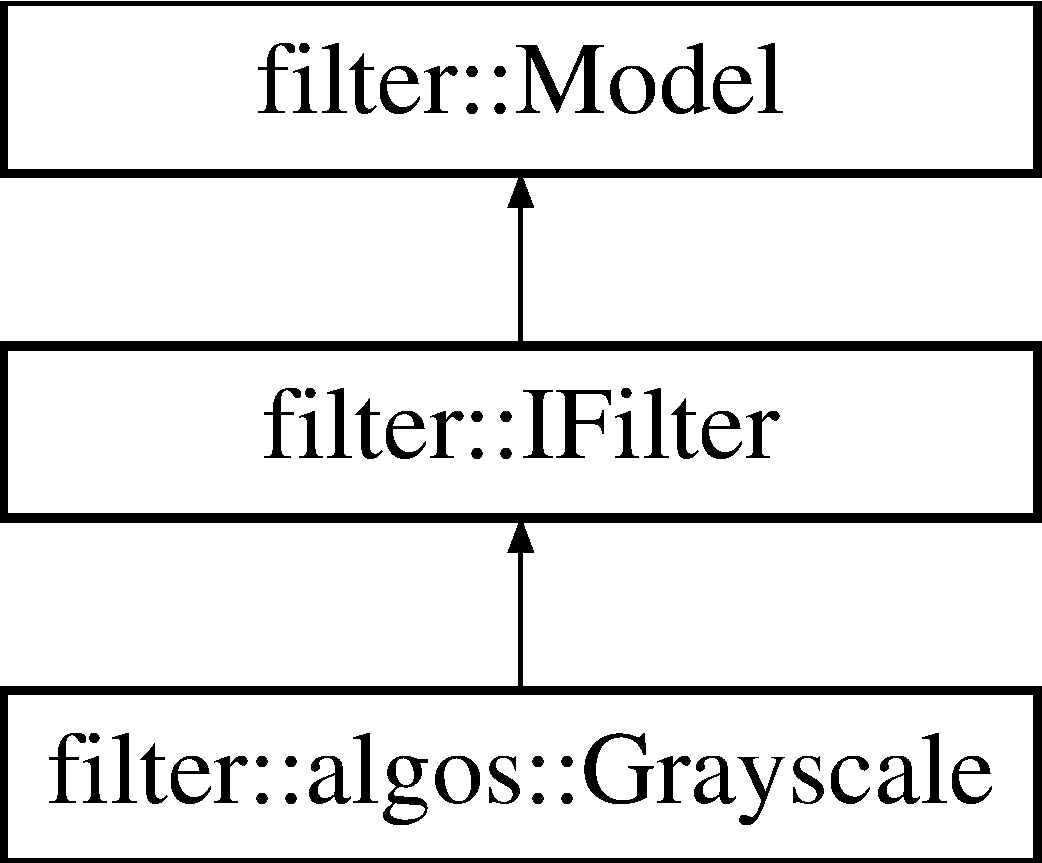
\includegraphics[height=3.000000cm]{db/dc6/classfilter_1_1algos_1_1_grayscale}
\end{center}
\end{figure}
\subsection*{Public Types}
\begin{DoxyCompactItemize}
\item 
\mbox{\Hypertarget{classfilter_1_1algos_1_1_grayscale_a2e7d023ab891781b079fbe57a4763130}\label{classfilter_1_1algos_1_1_grayscale_a2e7d023ab891781b079fbe57a4763130}} 
typedef \hyperlink{class_proxy_functor}{Proxy\+Functor}$<$ \hyperlink{classfilter_1_1algos_1_1_grayscale}{Grayscale} $>$ {\bfseries \+\_\+proxy\+Functor}
\item 
\mbox{\Hypertarget{classfilter_1_1algos_1_1_grayscale_a81fe6103c7c354a08eb74cad412bc397}\label{classfilter_1_1algos_1_1_grayscale_a81fe6103c7c354a08eb74cad412bc397}} 
typedef \hyperlink{classfilter_1_1algos_1_1_grayscale}{Grayscale} {\bfseries mytype}
\item 
\mbox{\Hypertarget{classfilter_1_1algos_1_1_grayscale_adcee9def3e07b6cdccc3ac07030a9c00}\label{classfilter_1_1algos_1_1_grayscale_adcee9def3e07b6cdccc3ac07030a9c00}} 
typedef char {\bfseries vartype\+\_\+\+\_\+unused}
\end{DoxyCompactItemize}
\subsection*{Public Member Functions}
\begin{DoxyCompactItemize}
\item 
\mbox{\Hypertarget{classfilter_1_1algos_1_1_grayscale_aeb8a50f6427cf9ce78ebe05741c9889f}\label{classfilter_1_1algos_1_1_grayscale_aeb8a50f6427cf9ce78ebe05741c9889f}} 
void {\bfseries set\+\_\+unused\+\_\+from\+\_\+json} (boost\+::property\+\_\+tree\+::ptree \&json\+Class)
\item 
\mbox{\Hypertarget{classfilter_1_1algos_1_1_grayscale_a9483a55300d3607f02db9610b547b03a}\label{classfilter_1_1algos_1_1_grayscale_a9483a55300d3607f02db9610b547b03a}} 
void {\bfseries set\+\_\+unused} (vartype\+\_\+\+\_\+unused \&\+\_\+\+\_\+unused)
\item 
\mbox{\Hypertarget{classfilter_1_1algos_1_1_grayscale_a9e7f79dd695f9f341ca145cbcac5ecf6}\label{classfilter_1_1algos_1_1_grayscale_a9e7f79dd695f9f341ca145cbcac5ecf6}} 
vartype\+\_\+\+\_\+unused {\bfseries get\+\_\+unused} ()
\item 
\mbox{\Hypertarget{classfilter_1_1algos_1_1_grayscale_a27fc11c8457b08d47fc2a97106b33d17}\label{classfilter_1_1algos_1_1_grayscale_a27fc11c8457b08d47fc2a97106b33d17}} 
void {\bfseries copy\+\_\+unused} (\hyperlink{classfilter_1_1algos_1_1_grayscale}{mytype} $\ast$instance)
\item 
\mbox{\Hypertarget{classfilter_1_1algos_1_1_grayscale_aa13c408105e3b4060e9370de8672acd0}\label{classfilter_1_1algos_1_1_grayscale_aa13c408105e3b4060e9370de8672acd0}} 
Hipe\+Status {\bfseries process} () override
\end{DoxyCompactItemize}
\subsection*{Public Attributes}
\begin{DoxyCompactItemize}
\item 
\mbox{\Hypertarget{classfilter_1_1algos_1_1_grayscale_ab0d84aad9d218a41f7cf738904fea76b}\label{classfilter_1_1algos_1_1_grayscale_ab0d84aad9d218a41f7cf738904fea76b}} 
char {\bfseries unused}
\end{DoxyCompactItemize}
\subsection*{Private Member Functions}
\begin{DoxyCompactItemize}
\item 
\mbox{\Hypertarget{classfilter_1_1algos_1_1_grayscale_a62dcc9ed5004761e4a0b7162f00e7df8}\label{classfilter_1_1algos_1_1_grayscale_a62dcc9ed5004761e4a0b7162f00e7df8}} 
virtual \hyperlink{classfilter_1_1data_1_1_connex_data_base}{data\+::\+Connex\+Data\+Base} \& {\bfseries get\+Connector} ()
\end{DoxyCompactItemize}
\subsection*{Private Attributes}
\begin{DoxyCompactItemize}
\item 
\mbox{\Hypertarget{classfilter_1_1algos_1_1_grayscale_a608895d90327d9fceb9164f8ac480ea2}\label{classfilter_1_1algos_1_1_grayscale_a608895d90327d9fceb9164f8ac480ea2}} 
\hyperlink{classfilter_1_1data_1_1_connex_data}{data\+::\+Connex\+Data}$<$ \hyperlink{classfilter_1_1data_1_1_image_data}{data\+::\+Image\+Data}, \hyperlink{classfilter_1_1data_1_1_image_data}{data\+::\+Image\+Data} $>$ {\bfseries \+\_\+connex\+Data}
\end{DoxyCompactItemize}
\subsection*{Additional Inherited Members}


The documentation for this class was generated from the following file\+:\begin{DoxyCompactItemize}
\item 
header/filter/\+Algos/Grayscale.\+h\end{DoxyCompactItemize}

\hypertarget{class_h264_live_server_media_session}{}\section{H264\+Live\+Server\+Media\+Session Class Reference}
\label{class_h264_live_server_media_session}\index{H264\+Live\+Server\+Media\+Session@{H264\+Live\+Server\+Media\+Session}}
Inheritance diagram for H264\+Live\+Server\+Media\+Session\+:\begin{figure}[H]
\begin{center}
\leavevmode
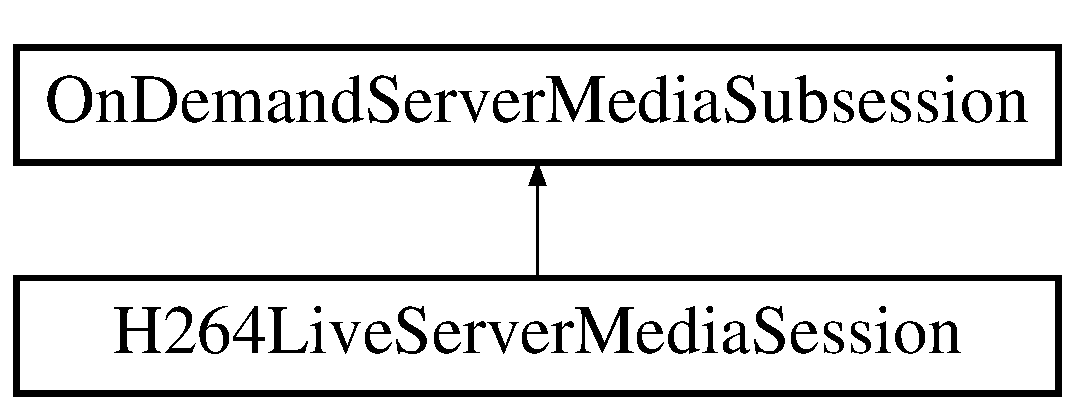
\includegraphics[height=2.000000cm]{df/d19/class_h264_live_server_media_session}
\end{center}
\end{figure}
\subsection*{Public Member Functions}
\begin{DoxyCompactItemize}
\item 
\mbox{\Hypertarget{class_h264_live_server_media_session_a425e58c77868ccf7652acb31357f0f6f}\label{class_h264_live_server_media_session_a425e58c77868ccf7652acb31357f0f6f}} 
void {\bfseries check\+For\+Aux\+S\+D\+P\+Line1} ()
\item 
\mbox{\Hypertarget{class_h264_live_server_media_session_a2837de6c0e367b8233d0d608446c7054}\label{class_h264_live_server_media_session_a2837de6c0e367b8233d0d608446c7054}} 
void {\bfseries after\+Playing\+Dummy1} ()
\end{DoxyCompactItemize}
\subsection*{Static Public Member Functions}
\begin{DoxyCompactItemize}
\item 
\mbox{\Hypertarget{class_h264_live_server_media_session_ac0b145c580d8a63a8fb61ba973d8e9b8}\label{class_h264_live_server_media_session_ac0b145c580d8a63a8fb61ba973d8e9b8}} 
static \hyperlink{class_h264_live_server_media_session}{H264\+Live\+Server\+Media\+Session} $\ast$ {\bfseries create\+New} (Usage\+Environment \&env, bool reuse\+First\+Source, \hyperlink{classcore_1_1queue_1_1_concurrent_queue}{core\+::queue\+::\+Concurrent\+Queue}$<$ \hyperlink{classfilter_1_1data_1_1_data}{filter\+::data\+::\+Data} $>$ \&concurrent\+\_\+queue)
\end{DoxyCompactItemize}
\subsection*{Protected Member Functions}
\begin{DoxyCompactItemize}
\item 
\mbox{\Hypertarget{class_h264_live_server_media_session_ad5be284c8c0b5e1b479ccb87f85b644a}\label{class_h264_live_server_media_session_ad5be284c8c0b5e1b479ccb87f85b644a}} 
{\bfseries H264\+Live\+Server\+Media\+Session} (Usage\+Environment \&env, bool reuse\+First\+Source, \hyperlink{classcore_1_1queue_1_1_concurrent_queue}{core\+::queue\+::\+Concurrent\+Queue}$<$ \hyperlink{classfilter_1_1data_1_1_data}{filter\+::data\+::\+Data} $>$ \&concurrent\+\_\+queue)
\item 
\mbox{\Hypertarget{class_h264_live_server_media_session_a436efe803a54a77a0ba8ea4420f439f3}\label{class_h264_live_server_media_session_a436efe803a54a77a0ba8ea4420f439f3}} 
void {\bfseries set\+Done\+Flag} ()
\item 
\mbox{\Hypertarget{class_h264_live_server_media_session_a19e96a64dda50b5ee07603976089b0ef}\label{class_h264_live_server_media_session_a19e96a64dda50b5ee07603976089b0ef}} 
virtual char const  $\ast$ {\bfseries get\+Aux\+S\+D\+P\+Line} (R\+T\+P\+Sink $\ast$rtp\+Sink, Framed\+Source $\ast$input\+Source)
\item 
\mbox{\Hypertarget{class_h264_live_server_media_session_a643871b4f55dfade6a4d71445d0f7a26}\label{class_h264_live_server_media_session_a643871b4f55dfade6a4d71445d0f7a26}} 
virtual Framed\+Source $\ast$ {\bfseries create\+New\+Stream\+Source} (unsigned client\+Session\+Id, unsigned \&est\+Bitrate)
\item 
\mbox{\Hypertarget{class_h264_live_server_media_session_a55ae1ef4c9316ce7925683a73fc52655}\label{class_h264_live_server_media_session_a55ae1ef4c9316ce7925683a73fc52655}} 
virtual R\+T\+P\+Sink $\ast$ {\bfseries create\+New\+R\+T\+P\+Sink} (Groupsock $\ast$rtp\+Groupsock, unsigned char rtp\+Payload\+Type\+If\+Dynamic, Framed\+Source $\ast$input\+Source)
\end{DoxyCompactItemize}
\subsection*{Private Attributes}
\begin{DoxyCompactItemize}
\item 
\mbox{\Hypertarget{class_h264_live_server_media_session_ac1b94afe60e2b966d99353836eee30b0}\label{class_h264_live_server_media_session_ac1b94afe60e2b966d99353836eee30b0}} 
char $\ast$ {\bfseries f\+Aux\+S\+D\+P\+Line}
\item 
\mbox{\Hypertarget{class_h264_live_server_media_session_a75e1b4db815f141d0014c04de1d6a811}\label{class_h264_live_server_media_session_a75e1b4db815f141d0014c04de1d6a811}} 
char {\bfseries f\+Done\+Flag}
\item 
\mbox{\Hypertarget{class_h264_live_server_media_session_ac0d59fbfc90f27eecb30cad7e9c2aa57}\label{class_h264_live_server_media_session_ac0d59fbfc90f27eecb30cad7e9c2aa57}} 
R\+T\+P\+Sink $\ast$ {\bfseries f\+Dummy\+Sink}
\item 
\mbox{\Hypertarget{class_h264_live_server_media_session_a2bf1fca74e15b552e82eaa6925834512}\label{class_h264_live_server_media_session_a2bf1fca74e15b552e82eaa6925834512}} 
\hyperlink{classcore_1_1queue_1_1_concurrent_queue}{core\+::queue\+::\+Concurrent\+Queue}$<$ \hyperlink{classfilter_1_1data_1_1_data}{filter\+::data\+::\+Data} $>$ \& {\bfseries \+\_\+concurrent\+\_\+queue}
\end{DoxyCompactItemize}


The documentation for this class was generated from the following files\+:\begin{DoxyCompactItemize}
\item 
header/streaming/H264\+Live\+Server\+Media\+Session.\+h\item 
source/streaming/H264\+Live\+Server\+Media\+Session.\+cpp\end{DoxyCompactItemize}

\hypertarget{class_hipe_exception}{}\section{Hipe\+Exception Class Reference}
\label{class_hipe_exception}\index{Hipe\+Exception@{Hipe\+Exception}}
Inheritance diagram for Hipe\+Exception\+:\begin{figure}[H]
\begin{center}
\leavevmode
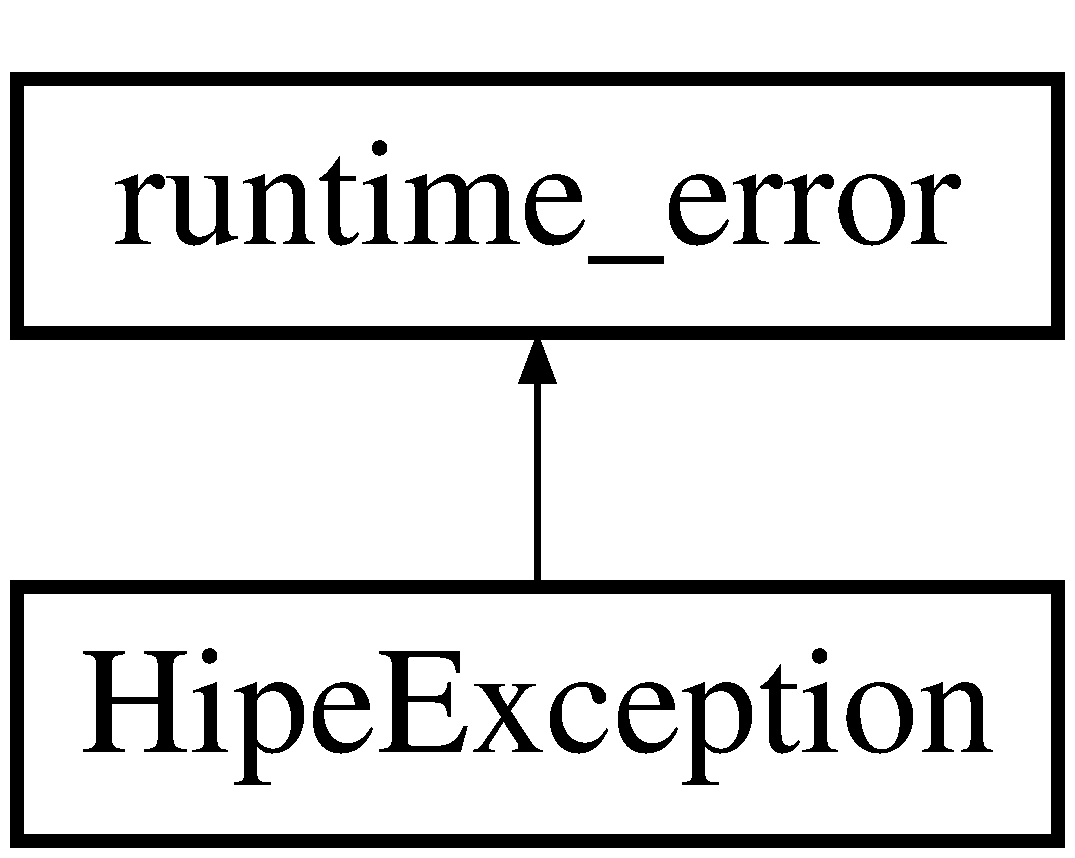
\includegraphics[height=2.000000cm]{d8/d9d/class_hipe_exception}
\end{center}
\end{figure}
\subsection*{Public Member Functions}
\begin{DoxyCompactItemize}
\item 
\mbox{\Hypertarget{class_hipe_exception_a61865350797373de27a596f09abc17b0}\label{class_hipe_exception_a61865350797373de27a596f09abc17b0}} 
{\bfseries Hipe\+Exception} (const char $\ast$message)
\item 
\mbox{\Hypertarget{class_hipe_exception_a61e2d2fb080e9f8926b3620cf7559c37}\label{class_hipe_exception_a61e2d2fb080e9f8926b3620cf7559c37}} 
{\bfseries Hipe\+Exception} (std\+::string message)
\end{DoxyCompactItemize}


The documentation for this class was generated from the following files\+:\begin{DoxyCompactItemize}
\item 
header/core/Hipe\+Exception.\+h\item 
source/core/Hipe\+Exception.\+cpp\end{DoxyCompactItemize}

\hypertarget{classhttp_1_1_http_params}{}\section{http\+:\+:Http\+Params Class Reference}
\label{classhttp_1_1_http_params}\index{http\+::\+Http\+Params@{http\+::\+Http\+Params}}


The documentation for this class was generated from the following file\+:\begin{DoxyCompactItemize}
\item 
header/http/Http\+Params.\+h\end{DoxyCompactItemize}

\hypertarget{classhttp_1_1_http_request}{}\section{http\+:\+:Http\+Request Class Reference}
\label{classhttp_1_1_http_request}\index{http\+::\+Http\+Request@{http\+::\+Http\+Request}}
\subsection*{Private Attributes}
\begin{DoxyCompactItemize}
\item 
\mbox{\Hypertarget{classhttp_1_1_http_request_a765f1ae5d1b14982169f3d7c2499f448}\label{classhttp_1_1_http_request_a765f1ae5d1b14982169f3d7c2499f448}} 
std\+::string {\bfseries \+\_\+json\+String}
\end{DoxyCompactItemize}


The documentation for this class was generated from the following file\+:\begin{DoxyCompactItemize}
\item 
header/http/Http\+Request.\+h\end{DoxyCompactItemize}

\hypertarget{classhttp_1_1_http_task}{}\section{http\+:\+:Http\+Task Class Reference}
\label{classhttp_1_1_http_task}\index{http\+::\+Http\+Task@{http\+::\+Http\+Task}}
\subsection*{Public Member Functions}
\begin{DoxyCompactItemize}
\item 
\mbox{\Hypertarget{classhttp_1_1_http_task_a19e0362421e3c9332460d99b0ab7f13e}\label{classhttp_1_1_http_task_a19e0362421e3c9332460d99b0ab7f13e}} 
{\bfseries Http\+Task} (std\+::shared\+\_\+ptr$<$ \hyperlink{classhttp_1_1_response}{Response}$<$ http\+::\+H\+T\+TP $>$$>$ \&response, std\+::shared\+\_\+ptr$<$ \hyperlink{classhttp_1_1_request}{http\+::\+Request}$<$ http\+::\+H\+T\+TP $>$$>$ \&request)
\item 
\mbox{\Hypertarget{classhttp_1_1_http_task_a2b62fcf83f5ea39cf514019433fba8ae}\label{classhttp_1_1_http_task_a2b62fcf83f5ea39cf514019433fba8ae}} 
void {\bfseries run\+Task} ()
\end{DoxyCompactItemize}
\subsection*{Static Public Attributes}
\begin{DoxyCompactItemize}
\item 
\mbox{\Hypertarget{classhttp_1_1_http_task_a7aba260b3b0a6d5618562e04c6641179}\label{classhttp_1_1_http_task_a7aba260b3b0a6d5618562e04c6641179}} 
static \hyperlink{classcore_1_1_logger}{core\+::\+Logger} {\bfseries logger} = core\+::set\+Class\+Name\+Attribute(\char`\"{}Http\+Task\char`\"{})
\end{DoxyCompactItemize}
\subsection*{Private Attributes}
\begin{DoxyCompactItemize}
\item 
\mbox{\Hypertarget{classhttp_1_1_http_task_af69a2447db2559b701847ab74fbac643}\label{classhttp_1_1_http_task_af69a2447db2559b701847ab74fbac643}} 
std\+::shared\+\_\+ptr$<$ \hyperlink{classhttp_1_1_response}{Response}$<$ http\+::\+H\+T\+TP $>$ $>$ \& {\bfseries \+\_\+response}
\item 
\mbox{\Hypertarget{classhttp_1_1_http_task_a1065dfd47fc586f4f73c1d2c9ca8abc6}\label{classhttp_1_1_http_task_a1065dfd47fc586f4f73c1d2c9ca8abc6}} 
std\+::shared\+\_\+ptr$<$ \hyperlink{classhttp_1_1_request}{Request}$<$ http\+::\+H\+T\+TP $>$ $>$ \& {\bfseries \+\_\+request}
\end{DoxyCompactItemize}


The documentation for this class was generated from the following files\+:\begin{DoxyCompactItemize}
\item 
header/http/Http\+Task.\+h\item 
source/http/Http\+Task.\+cpp\end{DoxyCompactItemize}

\hypertarget{classfilter_1_1algos_1_1_i_d_plate_cropper}{}\section{filter\+:\+:algos\+:\+:I\+D\+Plate\+Cropper Class Reference}
\label{classfilter_1_1algos_1_1_i_d_plate_cropper}\index{filter\+::algos\+::\+I\+D\+Plate\+Cropper@{filter\+::algos\+::\+I\+D\+Plate\+Cropper}}


The \hyperlink{classfilter_1_1algos_1_1_i_d_plate_cropper}{I\+D\+Plate\+Cropper} filter will try to find an ID plate in an image and crop it.  




{\ttfamily \#include $<$I\+D\+Plate\+Cropper.\+h$>$}

Inheritance diagram for filter\+:\+:algos\+:\+:I\+D\+Plate\+Cropper\+:\begin{figure}[H]
\begin{center}
\leavevmode
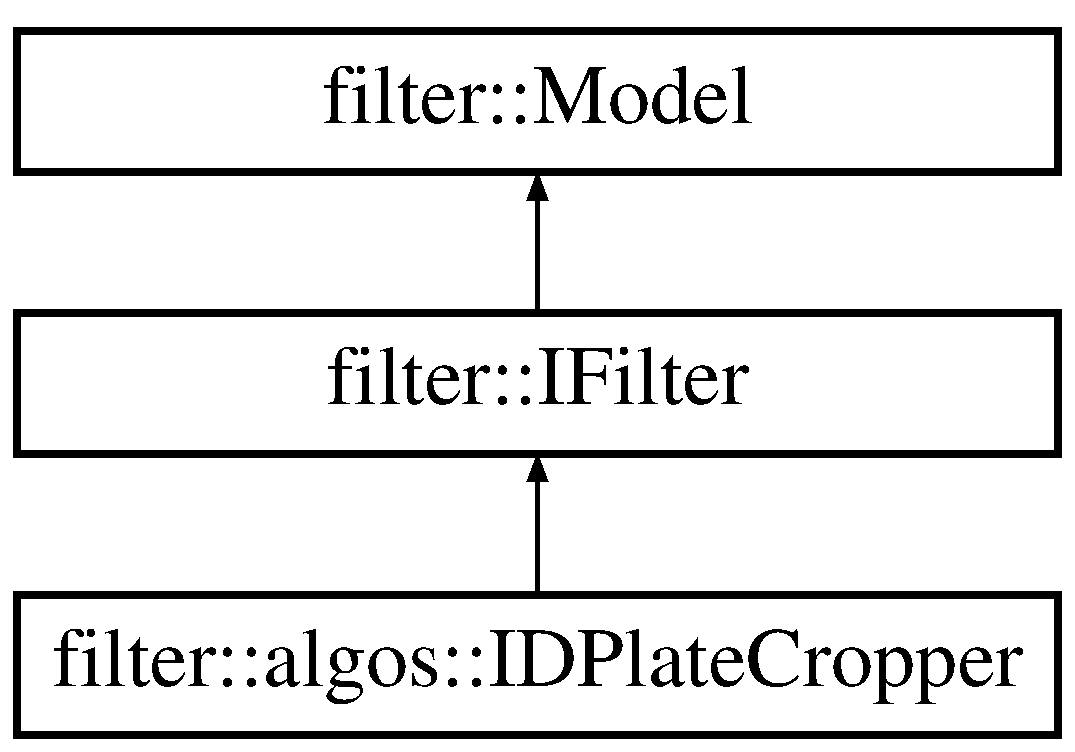
\includegraphics[height=3.000000cm]{d9/d7a/classfilter_1_1algos_1_1_i_d_plate_cropper}
\end{center}
\end{figure}
\subsection*{Public Types}
\begin{DoxyCompactItemize}
\item 
\mbox{\Hypertarget{classfilter_1_1algos_1_1_i_d_plate_cropper_a8fd987b6893bcdec4e3d3df4068f2082}\label{classfilter_1_1algos_1_1_i_d_plate_cropper_a8fd987b6893bcdec4e3d3df4068f2082}} 
typedef \hyperlink{class_proxy_functor}{Proxy\+Functor}$<$ \hyperlink{classfilter_1_1algos_1_1_i_d_plate_cropper}{I\+D\+Plate\+Cropper} $>$ {\bfseries \+\_\+proxy\+Functor}
\item 
\mbox{\Hypertarget{classfilter_1_1algos_1_1_i_d_plate_cropper_a905ed1c4871fc5ffbfd999e39e08ccdc}\label{classfilter_1_1algos_1_1_i_d_plate_cropper_a905ed1c4871fc5ffbfd999e39e08ccdc}} 
typedef \hyperlink{classfilter_1_1algos_1_1_i_d_plate_cropper}{I\+D\+Plate\+Cropper} {\bfseries mytype}
\item 
\mbox{\Hypertarget{classfilter_1_1algos_1_1_i_d_plate_cropper_a4bdb50418aed64d913c226109e572425}\label{classfilter_1_1algos_1_1_i_d_plate_cropper_a4bdb50418aed64d913c226109e572425}} 
typedef bool {\bfseries vartype\+\_\+\+\_\+use\+G\+PU}
\item 
\mbox{\Hypertarget{classfilter_1_1algos_1_1_i_d_plate_cropper_a67405e8caf6bbd909e668339ec5b1ffd}\label{classfilter_1_1algos_1_1_i_d_plate_cropper_a67405e8caf6bbd909e668339ec5b1ffd}} 
typedef int {\bfseries vartype\+\_\+\+\_\+bfilter\+Passes}
\item 
\mbox{\Hypertarget{classfilter_1_1algos_1_1_i_d_plate_cropper_a9bd582e8e93628ed0204601a50433a34}\label{classfilter_1_1algos_1_1_i_d_plate_cropper_a9bd582e8e93628ed0204601a50433a34}} 
typedef int {\bfseries vartype\+\_\+\+\_\+\+\_\+debug}
\end{DoxyCompactItemize}
\subsection*{Public Member Functions}
\begin{DoxyCompactItemize}
\item 
\mbox{\Hypertarget{classfilter_1_1algos_1_1_i_d_plate_cropper_a58946dadd862be0ab9df163c27e8e4a2}\label{classfilter_1_1algos_1_1_i_d_plate_cropper_a58946dadd862be0ab9df163c27e8e4a2}} 
void {\bfseries set\+\_\+use\+G\+P\+U\+\_\+from\+\_\+json} (boost\+::property\+\_\+tree\+::ptree \&json\+Class)
\item 
\mbox{\Hypertarget{classfilter_1_1algos_1_1_i_d_plate_cropper_aa85b6c55f8363fbca1ea32eceaf1f52a}\label{classfilter_1_1algos_1_1_i_d_plate_cropper_aa85b6c55f8363fbca1ea32eceaf1f52a}} 
void {\bfseries set\+\_\+use\+G\+PU} (vartype\+\_\+\+\_\+use\+G\+PU \&\+\_\+\+\_\+use\+G\+PU)
\item 
\mbox{\Hypertarget{classfilter_1_1algos_1_1_i_d_plate_cropper_a62f7abdafc518e5536b1f87381bb7f67}\label{classfilter_1_1algos_1_1_i_d_plate_cropper_a62f7abdafc518e5536b1f87381bb7f67}} 
vartype\+\_\+\+\_\+use\+G\+PU {\bfseries get\+\_\+use\+G\+PU} ()
\item 
\mbox{\Hypertarget{classfilter_1_1algos_1_1_i_d_plate_cropper_a20ae81c7b13f2667f1764a8dd18de342}\label{classfilter_1_1algos_1_1_i_d_plate_cropper_a20ae81c7b13f2667f1764a8dd18de342}} 
void {\bfseries copy\+\_\+use\+G\+PU} (\hyperlink{classfilter_1_1algos_1_1_i_d_plate_cropper}{mytype} $\ast$instance)
\item 
\mbox{\Hypertarget{classfilter_1_1algos_1_1_i_d_plate_cropper_a4f80adf95c51d81697ebe16ee4e1b4d6}\label{classfilter_1_1algos_1_1_i_d_plate_cropper_a4f80adf95c51d81697ebe16ee4e1b4d6}} 
void {\bfseries set\+\_\+bfilter\+Passes\+\_\+from\+\_\+json} (boost\+::property\+\_\+tree\+::ptree \&json\+Class)
\item 
\mbox{\Hypertarget{classfilter_1_1algos_1_1_i_d_plate_cropper_a63825b6bcf0e9b8eb461b6d655810869}\label{classfilter_1_1algos_1_1_i_d_plate_cropper_a63825b6bcf0e9b8eb461b6d655810869}} 
void {\bfseries set\+\_\+bfilter\+Passes} (vartype\+\_\+\+\_\+bfilter\+Passes \&\+\_\+\+\_\+bfilter\+Passes)
\item 
\mbox{\Hypertarget{classfilter_1_1algos_1_1_i_d_plate_cropper_a54577939e0972053ca5d93411d876052}\label{classfilter_1_1algos_1_1_i_d_plate_cropper_a54577939e0972053ca5d93411d876052}} 
vartype\+\_\+\+\_\+bfilter\+Passes {\bfseries get\+\_\+bfilter\+Passes} ()
\item 
\mbox{\Hypertarget{classfilter_1_1algos_1_1_i_d_plate_cropper_abed5bdc471210863b378dbf17814d163}\label{classfilter_1_1algos_1_1_i_d_plate_cropper_abed5bdc471210863b378dbf17814d163}} 
void {\bfseries copy\+\_\+bfilter\+Passes} (\hyperlink{classfilter_1_1algos_1_1_i_d_plate_cropper}{mytype} $\ast$instance)
\item 
\mbox{\Hypertarget{classfilter_1_1algos_1_1_i_d_plate_cropper_aa1308114577b67787e62c1e5bbb8c10d}\label{classfilter_1_1algos_1_1_i_d_plate_cropper_aa1308114577b67787e62c1e5bbb8c10d}} 
void {\bfseries set\+\_\+\+\_\+debug\+\_\+from\+\_\+json} (boost\+::property\+\_\+tree\+::ptree \&json\+Class)
\item 
\mbox{\Hypertarget{classfilter_1_1algos_1_1_i_d_plate_cropper_a5d337b622b0f3dbc064938f522b972f2}\label{classfilter_1_1algos_1_1_i_d_plate_cropper_a5d337b622b0f3dbc064938f522b972f2}} 
void {\bfseries set\+\_\+\+\_\+debug} (vartype\+\_\+\+\_\+\+\_\+debug \&\+\_\+\+\_\+\+\_\+debug)
\item 
\mbox{\Hypertarget{classfilter_1_1algos_1_1_i_d_plate_cropper_a86c4c545ed09652aef9b766607e6a2d6}\label{classfilter_1_1algos_1_1_i_d_plate_cropper_a86c4c545ed09652aef9b766607e6a2d6}} 
vartype\+\_\+\+\_\+\+\_\+debug {\bfseries get\+\_\+\+\_\+debug} ()
\item 
\mbox{\Hypertarget{classfilter_1_1algos_1_1_i_d_plate_cropper_a49b9dd08e4e3a60152fce7884fe3efe5}\label{classfilter_1_1algos_1_1_i_d_plate_cropper_a49b9dd08e4e3a60152fce7884fe3efe5}} 
void {\bfseries copy\+\_\+\+\_\+debug} (\hyperlink{classfilter_1_1algos_1_1_i_d_plate_cropper}{mytype} $\ast$instance)
\item 
\mbox{\Hypertarget{classfilter_1_1algos_1_1_i_d_plate_cropper_a6e503940fb3fdd2f7cb863cbcf29207e}\label{classfilter_1_1algos_1_1_i_d_plate_cropper_a6e503940fb3fdd2f7cb863cbcf29207e}} 
Hipe\+Status {\bfseries process} () override
\end{DoxyCompactItemize}
\subsection*{Public Attributes}
\begin{DoxyCompactItemize}
\item 
bool \hyperlink{classfilter_1_1algos_1_1_i_d_plate_cropper_a4d72b1833fc13bc45ec68bb523a92195}{use\+G\+PU}
\item 
int \hyperlink{classfilter_1_1algos_1_1_i_d_plate_cropper_af30917d3c48a1911931de5801035da22}{bfilter\+Passes}
\item 
int \hyperlink{classfilter_1_1algos_1_1_i_d_plate_cropper_ad57b87a49b8e57f78559a91a97523e72}{\+\_\+debug}
\end{DoxyCompactItemize}
\subsection*{Private Member Functions}
\begin{DoxyCompactItemize}
\item 
\mbox{\Hypertarget{classfilter_1_1algos_1_1_i_d_plate_cropper_a13a1acc4ae917be6162040456094347a}\label{classfilter_1_1algos_1_1_i_d_plate_cropper_a13a1acc4ae917be6162040456094347a}} 
virtual \hyperlink{classfilter_1_1data_1_1_connex_data_base}{data\+::\+Connex\+Data\+Base} \& {\bfseries get\+Connector} ()
\item 
cv\+::\+Mat \hyperlink{classfilter_1_1algos_1_1_i_d_plate_cropper_a1ac43e82954727fc623910f8eb7260ca}{process\+Plate\+Image} (const cv\+::\+Mat \&plate\+Image)
\begin{DoxyCompactList}\small\item\em Preprocess the plate image by binarizing it then searching for blobs. The biggest one will be the R\+OI englobing the text area. \end{DoxyCompactList}\end{DoxyCompactItemize}
\subsection*{Private Attributes}
\begin{DoxyCompactItemize}
\item 
\mbox{\Hypertarget{classfilter_1_1algos_1_1_i_d_plate_cropper_aa003aba2f7ec0cc7d57f4ad9e82239bf}\label{classfilter_1_1algos_1_1_i_d_plate_cropper_aa003aba2f7ec0cc7d57f4ad9e82239bf}} 
\hyperlink{classfilter_1_1data_1_1_connex_data}{data\+::\+Connex\+Data}$<$ \hyperlink{classfilter_1_1data_1_1_image_data}{data\+::\+Image\+Data}, \hyperlink{classfilter_1_1data_1_1_image_data}{data\+::\+Image\+Data} $>$ {\bfseries \+\_\+connex\+Data}
\end{DoxyCompactItemize}
\subsection*{Additional Inherited Members}


\subsection{Member Function Documentation}
\mbox{\Hypertarget{classfilter_1_1algos_1_1_i_d_plate_cropper_a1ac43e82954727fc623910f8eb7260ca}\label{classfilter_1_1algos_1_1_i_d_plate_cropper_a1ac43e82954727fc623910f8eb7260ca}} 
\index{filter\+::algos\+::\+I\+D\+Plate\+Cropper@{filter\+::algos\+::\+I\+D\+Plate\+Cropper}!process\+Plate\+Image@{process\+Plate\+Image}}
\index{process\+Plate\+Image@{process\+Plate\+Image}!filter\+::algos\+::\+I\+D\+Plate\+Cropper@{filter\+::algos\+::\+I\+D\+Plate\+Cropper}}
\subsubsection{\texorpdfstring{process\+Plate\+Image()}{processPlateImage()}}
{\footnotesize\ttfamily cv\+::\+Mat filter\+::algos\+::\+I\+D\+Plate\+Cropper\+::process\+Plate\+Image (\begin{DoxyParamCaption}\item[{const cv\+::\+Mat \&}]{plate\+Image }\end{DoxyParamCaption})\hspace{0.3cm}{\ttfamily [private]}}


\begin{DoxyParams}{Parameters}
{\em plate\+Image} & The input plate image in color. \\
\hline
\end{DoxyParams}
\begin{DoxyReturn}{Returns}
A cropped color image of the found R\+OI englobing the text area. 
\end{DoxyReturn}


\subsection{Member Data Documentation}
\mbox{\Hypertarget{classfilter_1_1algos_1_1_i_d_plate_cropper_ad57b87a49b8e57f78559a91a97523e72}\label{classfilter_1_1algos_1_1_i_d_plate_cropper_ad57b87a49b8e57f78559a91a97523e72}} 
\index{filter\+::algos\+::\+I\+D\+Plate\+Cropper@{filter\+::algos\+::\+I\+D\+Plate\+Cropper}!\+\_\+debug@{\+\_\+debug}}
\index{\+\_\+debug@{\+\_\+debug}!filter\+::algos\+::\+I\+D\+Plate\+Cropper@{filter\+::algos\+::\+I\+D\+Plate\+Cropper}}
\subsubsection{\texorpdfstring{\+\_\+debug}{\_debug}}
{\footnotesize\ttfamily filter\+::algos\+::\+I\+D\+Plate\+Cropper\+::\+\_\+debug}

The desired debug level. The default level is 0 (disabled). A higher value will enable more debug informations. \mbox{\Hypertarget{classfilter_1_1algos_1_1_i_d_plate_cropper_af30917d3c48a1911931de5801035da22}\label{classfilter_1_1algos_1_1_i_d_plate_cropper_af30917d3c48a1911931de5801035da22}} 
\index{filter\+::algos\+::\+I\+D\+Plate\+Cropper@{filter\+::algos\+::\+I\+D\+Plate\+Cropper}!bfilter\+Passes@{bfilter\+Passes}}
\index{bfilter\+Passes@{bfilter\+Passes}!filter\+::algos\+::\+I\+D\+Plate\+Cropper@{filter\+::algos\+::\+I\+D\+Plate\+Cropper}}
\subsubsection{\texorpdfstring{bfilter\+Passes}{bfilterPasses}}
{\footnotesize\ttfamily filter\+::algos\+::\+I\+D\+Plate\+Cropper\+::bfilter\+Passes}

The desired number of times the bilateral filtering should be applied. \mbox{\Hypertarget{classfilter_1_1algos_1_1_i_d_plate_cropper_a4d72b1833fc13bc45ec68bb523a92195}\label{classfilter_1_1algos_1_1_i_d_plate_cropper_a4d72b1833fc13bc45ec68bb523a92195}} 
\index{filter\+::algos\+::\+I\+D\+Plate\+Cropper@{filter\+::algos\+::\+I\+D\+Plate\+Cropper}!use\+G\+PU@{use\+G\+PU}}
\index{use\+G\+PU@{use\+G\+PU}!filter\+::algos\+::\+I\+D\+Plate\+Cropper@{filter\+::algos\+::\+I\+D\+Plate\+Cropper}}
\subsubsection{\texorpdfstring{use\+G\+PU}{useGPU}}
{\footnotesize\ttfamily filter\+::algos\+::\+I\+D\+Plate\+Cropper\+::use\+G\+PU}

Should the G\+PU be used to apply the bilateral filtering or not. 

The documentation for this class was generated from the following files\+:\begin{DoxyCompactItemize}
\item 
header/filter/\+Algos/I\+D\+Plate\+Cropper.\+h\item 
source/filter/algos/I\+D\+Plate\+Cropper.\+cpp\end{DoxyCompactItemize}

\hypertarget{classfilter_1_1_algos_1_1_i_d_plate_identifier}{}\section{filter\+:\+:Algos\+:\+:I\+D\+Plate\+Identifier Class Reference}
\label{classfilter_1_1_algos_1_1_i_d_plate_identifier}\index{filter\+::\+Algos\+::\+I\+D\+Plate\+Identifier@{filter\+::\+Algos\+::\+I\+D\+Plate\+Identifier}}
Inheritance diagram for filter\+:\+:Algos\+:\+:I\+D\+Plate\+Identifier\+:\begin{figure}[H]
\begin{center}
\leavevmode
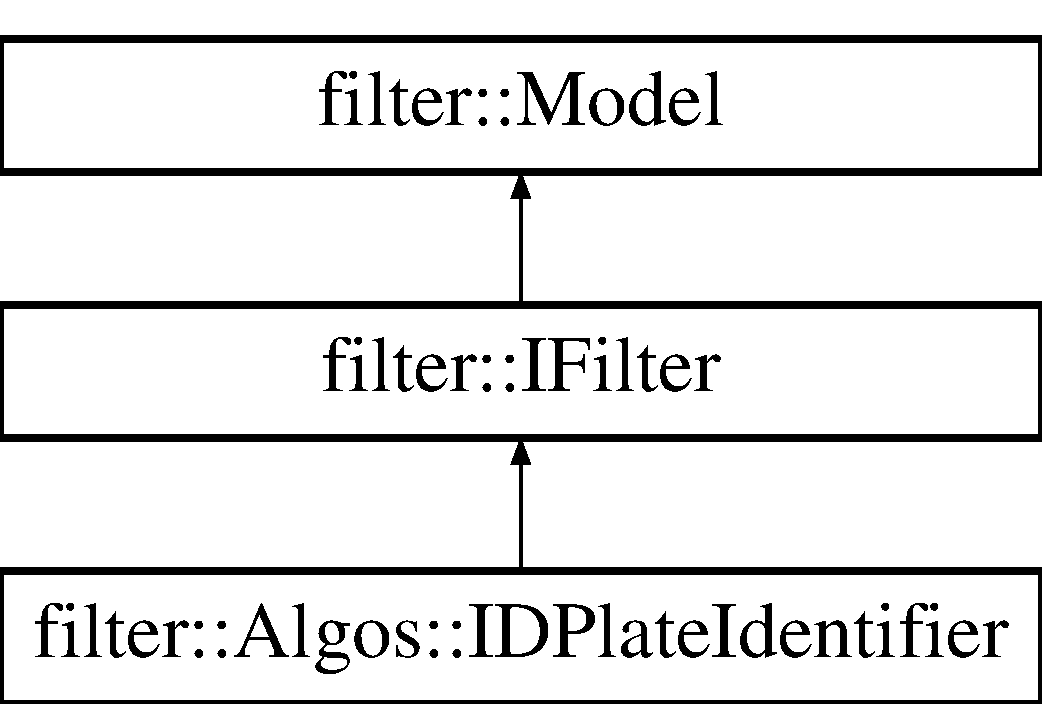
\includegraphics[height=3.000000cm]{dd/d88/classfilter_1_1_algos_1_1_i_d_plate_identifier}
\end{center}
\end{figure}
\subsection*{Public Types}
\begin{DoxyCompactItemize}
\item 
\mbox{\Hypertarget{classfilter_1_1_algos_1_1_i_d_plate_identifier_a8fbf5e351e89cf190bd5ac61a84f046e}\label{classfilter_1_1_algos_1_1_i_d_plate_identifier_a8fbf5e351e89cf190bd5ac61a84f046e}} 
typedef \hyperlink{class_proxy_functor}{Proxy\+Functor}$<$ \hyperlink{classfilter_1_1_algos_1_1_i_d_plate_identifier}{I\+D\+Plate\+Identifier} $>$ {\bfseries \+\_\+proxy\+Functor}
\item 
\mbox{\Hypertarget{classfilter_1_1_algos_1_1_i_d_plate_identifier_a40ddb0cd6caa012ca9725e02a84095ca}\label{classfilter_1_1_algos_1_1_i_d_plate_identifier_a40ddb0cd6caa012ca9725e02a84095ca}} 
typedef \hyperlink{classfilter_1_1_algos_1_1_i_d_plate_identifier}{I\+D\+Plate\+Identifier} {\bfseries mytype}
\item 
\mbox{\Hypertarget{classfilter_1_1_algos_1_1_i_d_plate_identifier_af2939dcabdec9e17ae7440fef2ddf0c3}\label{classfilter_1_1_algos_1_1_i_d_plate_identifier_af2939dcabdec9e17ae7440fef2ddf0c3}} 
typedef int {\bfseries vartype\+\_\+\+\_\+\+\_\+debug}
\item 
\mbox{\Hypertarget{classfilter_1_1_algos_1_1_i_d_plate_identifier_a75d336850af77f83df6f434db5d29cdd}\label{classfilter_1_1_algos_1_1_i_d_plate_identifier_a75d336850af77f83df6f434db5d29cdd}} 
typedef double {\bfseries vartype\+\_\+\+\_\+min\+X\+Pos}
\item 
\mbox{\Hypertarget{classfilter_1_1_algos_1_1_i_d_plate_identifier_af1247907c28c5486ef40cb523c2a2f3e}\label{classfilter_1_1_algos_1_1_i_d_plate_identifier_af1247907c28c5486ef40cb523c2a2f3e}} 
typedef double {\bfseries vartype\+\_\+\+\_\+max\+X\+Pos}
\item 
\mbox{\Hypertarget{classfilter_1_1_algos_1_1_i_d_plate_identifier_a2365f3f805c16d8aae5a5763ef51d051}\label{classfilter_1_1_algos_1_1_i_d_plate_identifier_a2365f3f805c16d8aae5a5763ef51d051}} 
typedef int {\bfseries vartype\+\_\+\+\_\+min\+Lines}
\item 
\mbox{\Hypertarget{classfilter_1_1_algos_1_1_i_d_plate_identifier_ad3ed91d7b11281fb648cac0aa7edd80a}\label{classfilter_1_1_algos_1_1_i_d_plate_identifier_ad3ed91d7b11281fb648cac0aa7edd80a}} 
typedef double {\bfseries vartype\+\_\+\+\_\+ratioY}
\item 
\mbox{\Hypertarget{classfilter_1_1_algos_1_1_i_d_plate_identifier_ad68832dbcdd687a1b70369ab0e130f20}\label{classfilter_1_1_algos_1_1_i_d_plate_identifier_ad68832dbcdd687a1b70369ab0e130f20}} 
typedef double {\bfseries vartype\+\_\+\+\_\+ratio\+Min\+Area}
\item 
\mbox{\Hypertarget{classfilter_1_1_algos_1_1_i_d_plate_identifier_a15ba4c80cff73437d0d721060c87e10c}\label{classfilter_1_1_algos_1_1_i_d_plate_identifier_a15ba4c80cff73437d0d721060c87e10c}} 
typedef double {\bfseries vartype\+\_\+\+\_\+ratio\+Max\+Area}
\end{DoxyCompactItemize}
\subsection*{Public Member Functions}
\begin{DoxyCompactItemize}
\item 
\mbox{\Hypertarget{classfilter_1_1_algos_1_1_i_d_plate_identifier_abe8d1115a3baf8dc7de4f7281bfd11ff}\label{classfilter_1_1_algos_1_1_i_d_plate_identifier_abe8d1115a3baf8dc7de4f7281bfd11ff}} 
void {\bfseries set\+\_\+\+\_\+debug\+\_\+from\+\_\+json} (boost\+::property\+\_\+tree\+::ptree \&json\+Class)
\item 
\mbox{\Hypertarget{classfilter_1_1_algos_1_1_i_d_plate_identifier_a956dc97af1dc492118f33c77cb4df76c}\label{classfilter_1_1_algos_1_1_i_d_plate_identifier_a956dc97af1dc492118f33c77cb4df76c}} 
void {\bfseries set\+\_\+\+\_\+debug} (vartype\+\_\+\+\_\+\+\_\+debug \&\+\_\+\+\_\+\+\_\+debug)
\item 
\mbox{\Hypertarget{classfilter_1_1_algos_1_1_i_d_plate_identifier_a00bb26115e8c0f4e98284e6e285c210a}\label{classfilter_1_1_algos_1_1_i_d_plate_identifier_a00bb26115e8c0f4e98284e6e285c210a}} 
vartype\+\_\+\+\_\+\+\_\+debug {\bfseries get\+\_\+\+\_\+debug} ()
\item 
\mbox{\Hypertarget{classfilter_1_1_algos_1_1_i_d_plate_identifier_a2e62e431fa39123fe33cd16192e3d8df}\label{classfilter_1_1_algos_1_1_i_d_plate_identifier_a2e62e431fa39123fe33cd16192e3d8df}} 
void {\bfseries copy\+\_\+\+\_\+debug} (\hyperlink{classfilter_1_1_algos_1_1_i_d_plate_identifier}{mytype} $\ast$instance)
\item 
\mbox{\Hypertarget{classfilter_1_1_algos_1_1_i_d_plate_identifier_a33928c486cf761ce0e309c627495500d}\label{classfilter_1_1_algos_1_1_i_d_plate_identifier_a33928c486cf761ce0e309c627495500d}} 
void {\bfseries set\+\_\+min\+X\+Pos\+\_\+from\+\_\+json} (boost\+::property\+\_\+tree\+::ptree \&json\+Class)
\item 
\mbox{\Hypertarget{classfilter_1_1_algos_1_1_i_d_plate_identifier_a07f1dad081b2d7333c798882073161e3}\label{classfilter_1_1_algos_1_1_i_d_plate_identifier_a07f1dad081b2d7333c798882073161e3}} 
void {\bfseries set\+\_\+min\+X\+Pos} (vartype\+\_\+\+\_\+min\+X\+Pos \&\+\_\+\+\_\+min\+X\+Pos)
\item 
\mbox{\Hypertarget{classfilter_1_1_algos_1_1_i_d_plate_identifier_ab86838092a2625a0fe1ec171905e938b}\label{classfilter_1_1_algos_1_1_i_d_plate_identifier_ab86838092a2625a0fe1ec171905e938b}} 
vartype\+\_\+\+\_\+min\+X\+Pos {\bfseries get\+\_\+min\+X\+Pos} ()
\item 
\mbox{\Hypertarget{classfilter_1_1_algos_1_1_i_d_plate_identifier_ac1c49fff537cee13c5331e98edd3aabb}\label{classfilter_1_1_algos_1_1_i_d_plate_identifier_ac1c49fff537cee13c5331e98edd3aabb}} 
void {\bfseries copy\+\_\+min\+X\+Pos} (\hyperlink{classfilter_1_1_algos_1_1_i_d_plate_identifier}{mytype} $\ast$instance)
\item 
\mbox{\Hypertarget{classfilter_1_1_algos_1_1_i_d_plate_identifier_a64b6955fc643e26f139c7df6ce7aec17}\label{classfilter_1_1_algos_1_1_i_d_plate_identifier_a64b6955fc643e26f139c7df6ce7aec17}} 
void {\bfseries set\+\_\+max\+X\+Pos\+\_\+from\+\_\+json} (boost\+::property\+\_\+tree\+::ptree \&json\+Class)
\item 
\mbox{\Hypertarget{classfilter_1_1_algos_1_1_i_d_plate_identifier_ab2efb805c4b3c62006573f219a1490f3}\label{classfilter_1_1_algos_1_1_i_d_plate_identifier_ab2efb805c4b3c62006573f219a1490f3}} 
void {\bfseries set\+\_\+max\+X\+Pos} (vartype\+\_\+\+\_\+max\+X\+Pos \&\+\_\+\+\_\+max\+X\+Pos)
\item 
\mbox{\Hypertarget{classfilter_1_1_algos_1_1_i_d_plate_identifier_af7e24241704e6d4cf8350ea8fed0072d}\label{classfilter_1_1_algos_1_1_i_d_plate_identifier_af7e24241704e6d4cf8350ea8fed0072d}} 
vartype\+\_\+\+\_\+max\+X\+Pos {\bfseries get\+\_\+max\+X\+Pos} ()
\item 
\mbox{\Hypertarget{classfilter_1_1_algos_1_1_i_d_plate_identifier_ac3ed41714a3a3864c992ce9f84ab9c4d}\label{classfilter_1_1_algos_1_1_i_d_plate_identifier_ac3ed41714a3a3864c992ce9f84ab9c4d}} 
void {\bfseries copy\+\_\+max\+X\+Pos} (\hyperlink{classfilter_1_1_algos_1_1_i_d_plate_identifier}{mytype} $\ast$instance)
\item 
\mbox{\Hypertarget{classfilter_1_1_algos_1_1_i_d_plate_identifier_a92b563d76274cab723d7e5e33bc499b2}\label{classfilter_1_1_algos_1_1_i_d_plate_identifier_a92b563d76274cab723d7e5e33bc499b2}} 
void {\bfseries set\+\_\+min\+Lines\+\_\+from\+\_\+json} (boost\+::property\+\_\+tree\+::ptree \&json\+Class)
\item 
\mbox{\Hypertarget{classfilter_1_1_algos_1_1_i_d_plate_identifier_a74a641ed0945592bfb351eee3b8e9a42}\label{classfilter_1_1_algos_1_1_i_d_plate_identifier_a74a641ed0945592bfb351eee3b8e9a42}} 
void {\bfseries set\+\_\+min\+Lines} (vartype\+\_\+\+\_\+min\+Lines \&\+\_\+\+\_\+min\+Lines)
\item 
\mbox{\Hypertarget{classfilter_1_1_algos_1_1_i_d_plate_identifier_a5e224f6ac242bd8a1513285105029d0c}\label{classfilter_1_1_algos_1_1_i_d_plate_identifier_a5e224f6ac242bd8a1513285105029d0c}} 
vartype\+\_\+\+\_\+min\+Lines {\bfseries get\+\_\+min\+Lines} ()
\item 
\mbox{\Hypertarget{classfilter_1_1_algos_1_1_i_d_plate_identifier_a06354f9ca9cfd78e7556a08c9cfb69cd}\label{classfilter_1_1_algos_1_1_i_d_plate_identifier_a06354f9ca9cfd78e7556a08c9cfb69cd}} 
void {\bfseries copy\+\_\+min\+Lines} (\hyperlink{classfilter_1_1_algos_1_1_i_d_plate_identifier}{mytype} $\ast$instance)
\item 
\mbox{\Hypertarget{classfilter_1_1_algos_1_1_i_d_plate_identifier_a406ae4f5da396e1184fd4740afc98687}\label{classfilter_1_1_algos_1_1_i_d_plate_identifier_a406ae4f5da396e1184fd4740afc98687}} 
void {\bfseries set\+\_\+ratio\+Y\+\_\+from\+\_\+json} (boost\+::property\+\_\+tree\+::ptree \&json\+Class)
\item 
\mbox{\Hypertarget{classfilter_1_1_algos_1_1_i_d_plate_identifier_a7f47586448147e2caea7c27b619c1e9c}\label{classfilter_1_1_algos_1_1_i_d_plate_identifier_a7f47586448147e2caea7c27b619c1e9c}} 
void {\bfseries set\+\_\+ratioY} (vartype\+\_\+\+\_\+ratioY \&\+\_\+\+\_\+ratioY)
\item 
\mbox{\Hypertarget{classfilter_1_1_algos_1_1_i_d_plate_identifier_af441b6411d5386d6752c63d49376ab52}\label{classfilter_1_1_algos_1_1_i_d_plate_identifier_af441b6411d5386d6752c63d49376ab52}} 
vartype\+\_\+\+\_\+ratioY {\bfseries get\+\_\+ratioY} ()
\item 
\mbox{\Hypertarget{classfilter_1_1_algos_1_1_i_d_plate_identifier_ae9fb4ae252f1d7d4d26cbd10335d893a}\label{classfilter_1_1_algos_1_1_i_d_plate_identifier_ae9fb4ae252f1d7d4d26cbd10335d893a}} 
void {\bfseries copy\+\_\+ratioY} (\hyperlink{classfilter_1_1_algos_1_1_i_d_plate_identifier}{mytype} $\ast$instance)
\item 
\mbox{\Hypertarget{classfilter_1_1_algos_1_1_i_d_plate_identifier_ace777a399097849804f2d339b30a5b7a}\label{classfilter_1_1_algos_1_1_i_d_plate_identifier_ace777a399097849804f2d339b30a5b7a}} 
void {\bfseries set\+\_\+ratio\+Min\+Area\+\_\+from\+\_\+json} (boost\+::property\+\_\+tree\+::ptree \&json\+Class)
\item 
\mbox{\Hypertarget{classfilter_1_1_algos_1_1_i_d_plate_identifier_ad15ea0a66206a0d8d01dac32f8a2800d}\label{classfilter_1_1_algos_1_1_i_d_plate_identifier_ad15ea0a66206a0d8d01dac32f8a2800d}} 
void {\bfseries set\+\_\+ratio\+Min\+Area} (vartype\+\_\+\+\_\+ratio\+Min\+Area \&\+\_\+\+\_\+ratio\+Min\+Area)
\item 
\mbox{\Hypertarget{classfilter_1_1_algos_1_1_i_d_plate_identifier_a7962c2926f2fd58145288c3e8d556883}\label{classfilter_1_1_algos_1_1_i_d_plate_identifier_a7962c2926f2fd58145288c3e8d556883}} 
vartype\+\_\+\+\_\+ratio\+Min\+Area {\bfseries get\+\_\+ratio\+Min\+Area} ()
\item 
\mbox{\Hypertarget{classfilter_1_1_algos_1_1_i_d_plate_identifier_af8d7d8137d96387556174021793c4573}\label{classfilter_1_1_algos_1_1_i_d_plate_identifier_af8d7d8137d96387556174021793c4573}} 
void {\bfseries copy\+\_\+ratio\+Min\+Area} (\hyperlink{classfilter_1_1_algos_1_1_i_d_plate_identifier}{mytype} $\ast$instance)
\item 
\mbox{\Hypertarget{classfilter_1_1_algos_1_1_i_d_plate_identifier_a38a1edfcc7b4441d62bb3e8bf8897586}\label{classfilter_1_1_algos_1_1_i_d_plate_identifier_a38a1edfcc7b4441d62bb3e8bf8897586}} 
void {\bfseries set\+\_\+ratio\+Max\+Area\+\_\+from\+\_\+json} (boost\+::property\+\_\+tree\+::ptree \&json\+Class)
\item 
\mbox{\Hypertarget{classfilter_1_1_algos_1_1_i_d_plate_identifier_a7d76948ef157014724acc7b5669e5c07}\label{classfilter_1_1_algos_1_1_i_d_plate_identifier_a7d76948ef157014724acc7b5669e5c07}} 
void {\bfseries set\+\_\+ratio\+Max\+Area} (vartype\+\_\+\+\_\+ratio\+Max\+Area \&\+\_\+\+\_\+ratio\+Max\+Area)
\item 
\mbox{\Hypertarget{classfilter_1_1_algos_1_1_i_d_plate_identifier_a1edee6c9b62dd712ce14a7156a7e90e8}\label{classfilter_1_1_algos_1_1_i_d_plate_identifier_a1edee6c9b62dd712ce14a7156a7e90e8}} 
vartype\+\_\+\+\_\+ratio\+Max\+Area {\bfseries get\+\_\+ratio\+Max\+Area} ()
\item 
\mbox{\Hypertarget{classfilter_1_1_algos_1_1_i_d_plate_identifier_a51e6e5eb561b2143b11444ff2006d035}\label{classfilter_1_1_algos_1_1_i_d_plate_identifier_a51e6e5eb561b2143b11444ff2006d035}} 
void {\bfseries copy\+\_\+ratio\+Max\+Area} (\hyperlink{classfilter_1_1_algos_1_1_i_d_plate_identifier}{mytype} $\ast$instance)
\item 
\mbox{\Hypertarget{classfilter_1_1_algos_1_1_i_d_plate_identifier_ad48d538a3a7edef63606dec214bd3532}\label{classfilter_1_1_algos_1_1_i_d_plate_identifier_ad48d538a3a7edef63606dec214bd3532}} 
Hipe\+Status {\bfseries process} () override
\end{DoxyCompactItemize}
\subsection*{Public Attributes}
\begin{DoxyCompactItemize}
\item 
int \hyperlink{classfilter_1_1_algos_1_1_i_d_plate_identifier_a77d38e1f10df45f9dc3ead39be484a27}{\+\_\+debug}
\item 
double \hyperlink{classfilter_1_1_algos_1_1_i_d_plate_identifier_ad2046fe20522a770d870f3acdfba95b6}{min\+X\+Pos}
\begin{DoxyCompactList}\small\item\em The \hyperlink{classfilter_1_1_algos_1_1_i_d_plate_identifier}{I\+D\+Plate\+Identifier} filter will handle the detection of the character of an ID plate then their recognition with machine learning. \end{DoxyCompactList}\item 
double \hyperlink{classfilter_1_1_algos_1_1_i_d_plate_identifier_a9915ef175c388d7078ff4e4d814dfadb}{max\+X\+Pos}
\item 
int \hyperlink{classfilter_1_1_algos_1_1_i_d_plate_identifier_a53b5e570450d77452422af3b47257d20}{min\+Lines}
\item 
double \hyperlink{classfilter_1_1_algos_1_1_i_d_plate_identifier_a46ee09888147ccaee5c647abe27ff7b0}{ratioY}
\item 
double \hyperlink{classfilter_1_1_algos_1_1_i_d_plate_identifier_a62e090f551fa2e5790a21a1235c13c8c}{ratio\+Min\+Area}
\item 
double \hyperlink{classfilter_1_1_algos_1_1_i_d_plate_identifier_a333762120ac6f91964ab75a80f0fba70}{ratio\+Max\+Area}
\end{DoxyCompactItemize}
\subsection*{Private Member Functions}
\begin{DoxyCompactItemize}
\item 
\mbox{\Hypertarget{classfilter_1_1_algos_1_1_i_d_plate_identifier_ae424cce182cf0d5dd65e0f4480da3936}\label{classfilter_1_1_algos_1_1_i_d_plate_identifier_ae424cce182cf0d5dd65e0f4480da3936}} 
virtual \hyperlink{classfilter_1_1data_1_1_connex_data_base}{data\+::\+Connex\+Data\+Base} \& {\bfseries get\+Connector} ()
\item 
cv\+::\+Mat \hyperlink{classfilter_1_1_algos_1_1_i_d_plate_identifier_a4ce2afa02689d7047310c64907cc40a4}{preprocess\+Image} (const cv\+::\+Mat \&plate\+Image)
\begin{DoxyCompactList}\small\item\em Preprocess an ID plate image to help the search of its characters contours. \end{DoxyCompactList}\item 
cv\+::\+Mat \hyperlink{classfilter_1_1_algos_1_1_i_d_plate_identifier_a9c438d1ec3c38527ab5a6faf925971b3}{crop\+R\+OI} (const cv\+::\+Mat \&image, const cv\+::\+Rect \&roi)
\begin{DoxyCompactList}\small\item\em A Wrapper function for cropping an image around a R\+OI. \end{DoxyCompactList}\item 
std\+::vector$<$ cv\+::\+Mat $>$ \hyperlink{classfilter_1_1_algos_1_1_i_d_plate_identifier_aa5e8c02fc1fc20cacaa1cc45610307e1}{crop\+R\+O\+Is} (const cv\+::\+Mat \&image, const std\+::vector$<$ cv\+::\+Rect $>$ \&rois)
\begin{DoxyCompactList}\small\item\em Batch process version of crop\+R\+OI. Crops an image around multiple R\+O\+Is. \end{DoxyCompactList}\item 
cv\+::\+Mat \hyperlink{classfilter_1_1_algos_1_1_i_d_plate_identifier_a954615df7d4060998e69fda73fa9a416}{create\+Output\+Image} (const cv\+::\+Mat \&plate\+Image, const std\+::vector$<$ cv\+::\+Rect $>$ \&characters\+Rects, const std\+::vector$<$ std\+::string $>$ \&characters\+Labels)
\begin{DoxyCompactList}\small\item\em From an image containing characters, generate another one with printed characters\+Labels text at characters\+Rects positions. \end{DoxyCompactList}\end{DoxyCompactItemize}
\subsection*{Private Attributes}
\begin{DoxyCompactItemize}
\item 
\mbox{\Hypertarget{classfilter_1_1_algos_1_1_i_d_plate_identifier_a67e49e1280f3d2facd2b53de56c22ee4}\label{classfilter_1_1_algos_1_1_i_d_plate_identifier_a67e49e1280f3d2facd2b53de56c22ee4}} 
\hyperlink{classfilter_1_1data_1_1_connex_data}{data\+::\+Connex\+Data}$<$ \hyperlink{classfilter_1_1data_1_1_image_data}{data\+::\+Image\+Data}, \hyperlink{classfilter_1_1data_1_1_image_data}{data\+::\+Image\+Data} $>$ {\bfseries \+\_\+connex\+Data}
\end{DoxyCompactItemize}
\subsection*{Additional Inherited Members}


\subsection{Member Function Documentation}
\mbox{\Hypertarget{classfilter_1_1_algos_1_1_i_d_plate_identifier_a954615df7d4060998e69fda73fa9a416}\label{classfilter_1_1_algos_1_1_i_d_plate_identifier_a954615df7d4060998e69fda73fa9a416}} 
\index{filter\+::\+Algos\+::\+I\+D\+Plate\+Identifier@{filter\+::\+Algos\+::\+I\+D\+Plate\+Identifier}!create\+Output\+Image@{create\+Output\+Image}}
\index{create\+Output\+Image@{create\+Output\+Image}!filter\+::\+Algos\+::\+I\+D\+Plate\+Identifier@{filter\+::\+Algos\+::\+I\+D\+Plate\+Identifier}}
\subsubsection{\texorpdfstring{create\+Output\+Image()}{createOutputImage()}}
{\footnotesize\ttfamily cv\+::\+Mat filter\+::\+Algos\+::\+I\+D\+Plate\+Identifier\+::create\+Output\+Image (\begin{DoxyParamCaption}\item[{const cv\+::\+Mat \&}]{plate\+Image,  }\item[{const std\+::vector$<$ cv\+::\+Rect $>$ \&}]{characters\+Rects,  }\item[{const std\+::vector$<$ std\+::string $>$ \&}]{characters\+Labels }\end{DoxyParamCaption})\hspace{0.3cm}{\ttfamily [private]}}


\begin{DoxyParams}{Parameters}
{\em plate\+Image} & The source image to use \\
\hline
{\em characters\+Rects} & The positions of the rects (where to put text) on the image \\
\hline
{\em characters\+Labels} & The text to put for each rect \\
\hline
\end{DoxyParams}
\begin{DoxyReturn}{Returns}
An image where the labels in characters\+Labels are drawn in their respective characters\+Rects position 
\end{DoxyReturn}
\mbox{\Hypertarget{classfilter_1_1_algos_1_1_i_d_plate_identifier_a9c438d1ec3c38527ab5a6faf925971b3}\label{classfilter_1_1_algos_1_1_i_d_plate_identifier_a9c438d1ec3c38527ab5a6faf925971b3}} 
\index{filter\+::\+Algos\+::\+I\+D\+Plate\+Identifier@{filter\+::\+Algos\+::\+I\+D\+Plate\+Identifier}!crop\+R\+OI@{crop\+R\+OI}}
\index{crop\+R\+OI@{crop\+R\+OI}!filter\+::\+Algos\+::\+I\+D\+Plate\+Identifier@{filter\+::\+Algos\+::\+I\+D\+Plate\+Identifier}}
\subsubsection{\texorpdfstring{crop\+R\+O\+I()}{cropROI()}}
{\footnotesize\ttfamily cv\+::\+Mat filter\+::\+Algos\+::\+I\+D\+Plate\+Identifier\+::crop\+R\+OI (\begin{DoxyParamCaption}\item[{const cv\+::\+Mat \&}]{image,  }\item[{const cv\+::\+Rect \&}]{roi }\end{DoxyParamCaption})\hspace{0.3cm}{\ttfamily [private]}}


\begin{DoxyParams}{Parameters}
{\em image} & The image on which the R\+OI will be extracted \\
\hline
{\em roi} & The R\+OI \\
\hline
\end{DoxyParams}
\begin{DoxyReturn}{Returns}
A new image containing only the cropped rect from the source image 
\end{DoxyReturn}
\mbox{\Hypertarget{classfilter_1_1_algos_1_1_i_d_plate_identifier_aa5e8c02fc1fc20cacaa1cc45610307e1}\label{classfilter_1_1_algos_1_1_i_d_plate_identifier_aa5e8c02fc1fc20cacaa1cc45610307e1}} 
\index{filter\+::\+Algos\+::\+I\+D\+Plate\+Identifier@{filter\+::\+Algos\+::\+I\+D\+Plate\+Identifier}!crop\+R\+O\+Is@{crop\+R\+O\+Is}}
\index{crop\+R\+O\+Is@{crop\+R\+O\+Is}!filter\+::\+Algos\+::\+I\+D\+Plate\+Identifier@{filter\+::\+Algos\+::\+I\+D\+Plate\+Identifier}}
\subsubsection{\texorpdfstring{crop\+R\+O\+Is()}{cropROIs()}}
{\footnotesize\ttfamily std\+::vector$<$ cv\+::\+Mat $>$ filter\+::\+Algos\+::\+I\+D\+Plate\+Identifier\+::crop\+R\+O\+Is (\begin{DoxyParamCaption}\item[{const cv\+::\+Mat \&}]{image,  }\item[{const std\+::vector$<$ cv\+::\+Rect $>$ \&}]{rois }\end{DoxyParamCaption})\hspace{0.3cm}{\ttfamily [private]}}


\begin{DoxyParams}{Parameters}
{\em image} & The image on which the R\+OI will be extracted \\
\hline
{\em rois} & The R\+O\+Is \\
\hline
\end{DoxyParams}
\begin{DoxyReturn}{Returns}
A container filled with all the new images containing only the cropped rects from the source image 
\end{DoxyReturn}
\mbox{\Hypertarget{classfilter_1_1_algos_1_1_i_d_plate_identifier_a4ce2afa02689d7047310c64907cc40a4}\label{classfilter_1_1_algos_1_1_i_d_plate_identifier_a4ce2afa02689d7047310c64907cc40a4}} 
\index{filter\+::\+Algos\+::\+I\+D\+Plate\+Identifier@{filter\+::\+Algos\+::\+I\+D\+Plate\+Identifier}!preprocess\+Image@{preprocess\+Image}}
\index{preprocess\+Image@{preprocess\+Image}!filter\+::\+Algos\+::\+I\+D\+Plate\+Identifier@{filter\+::\+Algos\+::\+I\+D\+Plate\+Identifier}}
\subsubsection{\texorpdfstring{preprocess\+Image()}{preprocessImage()}}
{\footnotesize\ttfamily cv\+::\+Mat filter\+::\+Algos\+::\+I\+D\+Plate\+Identifier\+::preprocess\+Image (\begin{DoxyParamCaption}\item[{const cv\+::\+Mat \&}]{plate\+Image }\end{DoxyParamCaption})\hspace{0.3cm}{\ttfamily [private]}}


\begin{DoxyParams}{Parameters}
{\em plate\+Image} & The color image of the plate \\
\hline
\end{DoxyParams}
\begin{DoxyReturn}{Returns}
Returns a preprocessed binary image where the characters are blackon a white background 
\end{DoxyReturn}


\subsection{Member Data Documentation}
\mbox{\Hypertarget{classfilter_1_1_algos_1_1_i_d_plate_identifier_a77d38e1f10df45f9dc3ead39be484a27}\label{classfilter_1_1_algos_1_1_i_d_plate_identifier_a77d38e1f10df45f9dc3ead39be484a27}} 
\index{filter\+::\+Algos\+::\+I\+D\+Plate\+Identifier@{filter\+::\+Algos\+::\+I\+D\+Plate\+Identifier}!\+\_\+debug@{\+\_\+debug}}
\index{\+\_\+debug@{\+\_\+debug}!filter\+::\+Algos\+::\+I\+D\+Plate\+Identifier@{filter\+::\+Algos\+::\+I\+D\+Plate\+Identifier}}
\subsubsection{\texorpdfstring{\+\_\+debug}{\_debug}}
{\footnotesize\ttfamily filter\+::\+Algos\+::\+I\+D\+Plate\+Identifier\+::\+\_\+debug}

The debug level to use to print informations and show images \mbox{\Hypertarget{classfilter_1_1_algos_1_1_i_d_plate_identifier_a9915ef175c388d7078ff4e4d814dfadb}\label{classfilter_1_1_algos_1_1_i_d_plate_identifier_a9915ef175c388d7078ff4e4d814dfadb}} 
\index{filter\+::\+Algos\+::\+I\+D\+Plate\+Identifier@{filter\+::\+Algos\+::\+I\+D\+Plate\+Identifier}!max\+X\+Pos@{max\+X\+Pos}}
\index{max\+X\+Pos@{max\+X\+Pos}!filter\+::\+Algos\+::\+I\+D\+Plate\+Identifier@{filter\+::\+Algos\+::\+I\+D\+Plate\+Identifier}}
\subsubsection{\texorpdfstring{max\+X\+Pos}{maxXPos}}
{\footnotesize\ttfamily filter\+::\+Algos\+::\+I\+D\+Plate\+Identifier\+::max\+X\+Pos}

The maximum position on the X Axis to stop searching for characters. \mbox{\Hypertarget{classfilter_1_1_algos_1_1_i_d_plate_identifier_a53b5e570450d77452422af3b47257d20}\label{classfilter_1_1_algos_1_1_i_d_plate_identifier_a53b5e570450d77452422af3b47257d20}} 
\index{filter\+::\+Algos\+::\+I\+D\+Plate\+Identifier@{filter\+::\+Algos\+::\+I\+D\+Plate\+Identifier}!min\+Lines@{min\+Lines}}
\index{min\+Lines@{min\+Lines}!filter\+::\+Algos\+::\+I\+D\+Plate\+Identifier@{filter\+::\+Algos\+::\+I\+D\+Plate\+Identifier}}
\subsubsection{\texorpdfstring{min\+Lines}{minLines}}
{\footnotesize\ttfamily filter\+::\+Algos\+::\+I\+D\+Plate\+Identifier\+::min\+Lines}

The minimum number of lines of text we can fit on the image(minimum number of lines means big character).Used to compute the minimum and maximum height a character can have. \mbox{\Hypertarget{classfilter_1_1_algos_1_1_i_d_plate_identifier_ad2046fe20522a770d870f3acdfba95b6}\label{classfilter_1_1_algos_1_1_i_d_plate_identifier_ad2046fe20522a770d870f3acdfba95b6}} 
\index{filter\+::\+Algos\+::\+I\+D\+Plate\+Identifier@{filter\+::\+Algos\+::\+I\+D\+Plate\+Identifier}!min\+X\+Pos@{min\+X\+Pos}}
\index{min\+X\+Pos@{min\+X\+Pos}!filter\+::\+Algos\+::\+I\+D\+Plate\+Identifier@{filter\+::\+Algos\+::\+I\+D\+Plate\+Identifier}}
\subsubsection{\texorpdfstring{min\+X\+Pos}{minXPos}}
{\footnotesize\ttfamily filter\+::\+Algos\+::\+I\+D\+Plate\+Identifier\+::min\+X\+Pos}

The minimum position on the X Axis to start searching for characters. \mbox{\Hypertarget{classfilter_1_1_algos_1_1_i_d_plate_identifier_a333762120ac6f91964ab75a80f0fba70}\label{classfilter_1_1_algos_1_1_i_d_plate_identifier_a333762120ac6f91964ab75a80f0fba70}} 
\index{filter\+::\+Algos\+::\+I\+D\+Plate\+Identifier@{filter\+::\+Algos\+::\+I\+D\+Plate\+Identifier}!ratio\+Max\+Area@{ratio\+Max\+Area}}
\index{ratio\+Max\+Area@{ratio\+Max\+Area}!filter\+::\+Algos\+::\+I\+D\+Plate\+Identifier@{filter\+::\+Algos\+::\+I\+D\+Plate\+Identifier}}
\subsubsection{\texorpdfstring{ratio\+Max\+Area}{ratioMaxArea}}
{\footnotesize\ttfamily filter\+::\+Algos\+::\+I\+D\+Plate\+Identifier\+::ratio\+Max\+Area}

The percentage of the average characters\textquotesingle{} area. Used to compute the maximum area a character can have to be valid. \mbox{\Hypertarget{classfilter_1_1_algos_1_1_i_d_plate_identifier_a62e090f551fa2e5790a21a1235c13c8c}\label{classfilter_1_1_algos_1_1_i_d_plate_identifier_a62e090f551fa2e5790a21a1235c13c8c}} 
\index{filter\+::\+Algos\+::\+I\+D\+Plate\+Identifier@{filter\+::\+Algos\+::\+I\+D\+Plate\+Identifier}!ratio\+Min\+Area@{ratio\+Min\+Area}}
\index{ratio\+Min\+Area@{ratio\+Min\+Area}!filter\+::\+Algos\+::\+I\+D\+Plate\+Identifier@{filter\+::\+Algos\+::\+I\+D\+Plate\+Identifier}}
\subsubsection{\texorpdfstring{ratio\+Min\+Area}{ratioMinArea}}
{\footnotesize\ttfamily filter\+::\+Algos\+::\+I\+D\+Plate\+Identifier\+::ratio\+Min\+Area}

The percentage of the average characters\textquotesingle{} area. Used to compute the minimum area a character can have to be valid. \mbox{\Hypertarget{classfilter_1_1_algos_1_1_i_d_plate_identifier_a46ee09888147ccaee5c647abe27ff7b0}\label{classfilter_1_1_algos_1_1_i_d_plate_identifier_a46ee09888147ccaee5c647abe27ff7b0}} 
\index{filter\+::\+Algos\+::\+I\+D\+Plate\+Identifier@{filter\+::\+Algos\+::\+I\+D\+Plate\+Identifier}!ratioY@{ratioY}}
\index{ratioY@{ratioY}!filter\+::\+Algos\+::\+I\+D\+Plate\+Identifier@{filter\+::\+Algos\+::\+I\+D\+Plate\+Identifier}}
\subsubsection{\texorpdfstring{ratioY}{ratioY}}
{\footnotesize\ttfamily filter\+::\+Algos\+::\+I\+D\+Plate\+Identifier\+::ratioY}

The percentage of the average characters\textquotesingle{} height. Every characters are not exactly centered on the same line. We use the ratio to search around this line. 

The documentation for this class was generated from the following files\+:\begin{DoxyCompactItemize}
\item 
header/filter/\+Algos/I\+D\+Plate\+Identifier.\+h\item 
source/filter/algos/I\+D\+Plate\+Identifier.\+cpp\end{DoxyCompactItemize}

\hypertarget{classfilter_1_1algos_1_1_i_d_plate_rectifier}{}\section{filter\+:\+:algos\+:\+:I\+D\+Plate\+Rectifier Class Reference}
\label{classfilter_1_1algos_1_1_i_d_plate_rectifier}\index{filter\+::algos\+::\+I\+D\+Plate\+Rectifier@{filter\+::algos\+::\+I\+D\+Plate\+Rectifier}}


The \hyperlink{classfilter_1_1algos_1_1_i_d_plate_rectifier}{I\+D\+Plate\+Rectifier} filter will try to extract the region of interest (where all the relative character are) of an ID plate and rework its perspective to make it easier to read.  




{\ttfamily \#include $<$I\+D\+Plate\+Rectifier.\+h$>$}

Inheritance diagram for filter\+:\+:algos\+:\+:I\+D\+Plate\+Rectifier\+:\begin{figure}[H]
\begin{center}
\leavevmode
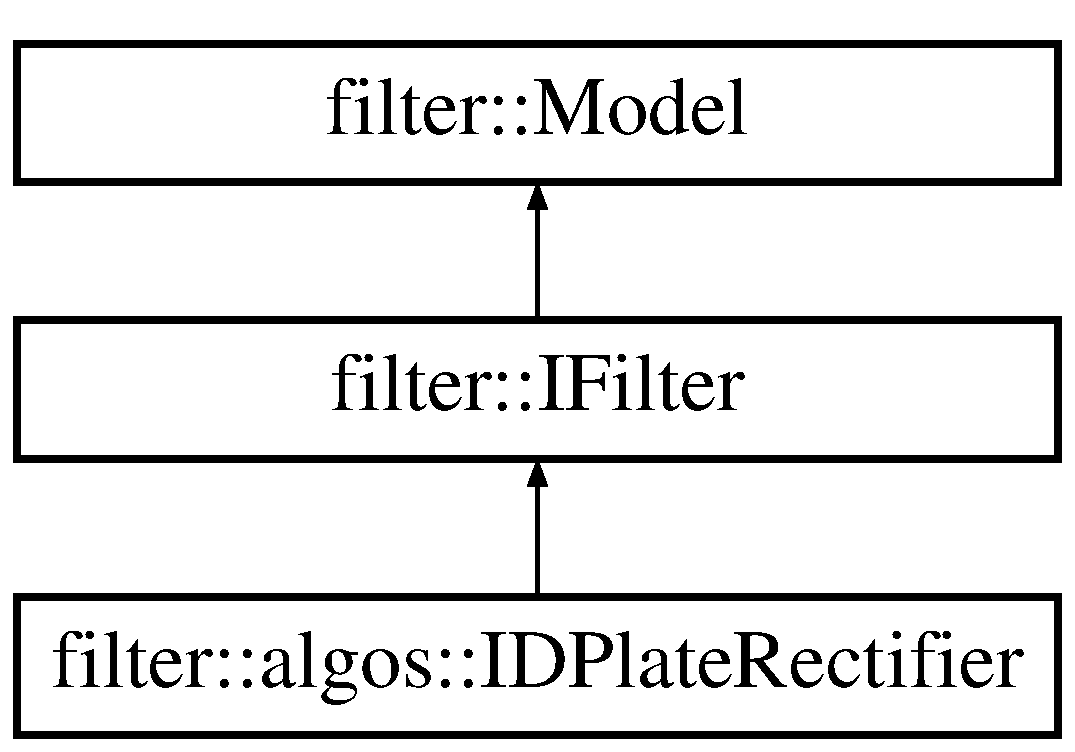
\includegraphics[height=3.000000cm]{d5/daf/classfilter_1_1algos_1_1_i_d_plate_rectifier}
\end{center}
\end{figure}
\subsection*{Public Types}
\begin{DoxyCompactItemize}
\item 
\mbox{\Hypertarget{classfilter_1_1algos_1_1_i_d_plate_rectifier_a079119de3cda8dfa38a76d06e5ceed8a}\label{classfilter_1_1algos_1_1_i_d_plate_rectifier_a079119de3cda8dfa38a76d06e5ceed8a}} 
typedef \hyperlink{class_proxy_functor}{Proxy\+Functor}$<$ \hyperlink{classfilter_1_1algos_1_1_i_d_plate_rectifier}{I\+D\+Plate\+Rectifier} $>$ {\bfseries \+\_\+proxy\+Functor}
\item 
\mbox{\Hypertarget{classfilter_1_1algos_1_1_i_d_plate_rectifier_acb4b673e736d6bef78b4128d6432df61}\label{classfilter_1_1algos_1_1_i_d_plate_rectifier_acb4b673e736d6bef78b4128d6432df61}} 
typedef \hyperlink{classfilter_1_1algos_1_1_i_d_plate_rectifier}{I\+D\+Plate\+Rectifier} {\bfseries mytype}
\item 
\mbox{\Hypertarget{classfilter_1_1algos_1_1_i_d_plate_rectifier_a3fea99ce502904063afbb703d7f47680}\label{classfilter_1_1algos_1_1_i_d_plate_rectifier_a3fea99ce502904063afbb703d7f47680}} 
typedef double {\bfseries vartype\+\_\+\+\_\+left\+Ratio}
\item 
\mbox{\Hypertarget{classfilter_1_1algos_1_1_i_d_plate_rectifier_a78876086c5a15b331433ad5a7643f60b}\label{classfilter_1_1algos_1_1_i_d_plate_rectifier_a78876086c5a15b331433ad5a7643f60b}} 
typedef double {\bfseries vartype\+\_\+\+\_\+right\+Ratio}
\item 
\mbox{\Hypertarget{classfilter_1_1algos_1_1_i_d_plate_rectifier_ae4fec9c71dbaa99898c9657ea38026d0}\label{classfilter_1_1algos_1_1_i_d_plate_rectifier_ae4fec9c71dbaa99898c9657ea38026d0}} 
typedef double {\bfseries vartype\+\_\+\+\_\+top\+Ratio}
\item 
\mbox{\Hypertarget{classfilter_1_1algos_1_1_i_d_plate_rectifier_ad4b3ccd17d6eda0009ed292dc0b8fa1b}\label{classfilter_1_1algos_1_1_i_d_plate_rectifier_ad4b3ccd17d6eda0009ed292dc0b8fa1b}} 
typedef int {\bfseries vartype\+\_\+\+\_\+\+\_\+debug}
\item 
\mbox{\Hypertarget{classfilter_1_1algos_1_1_i_d_plate_rectifier_a740bc26c7f66d34fb6c3d30024edc094}\label{classfilter_1_1algos_1_1_i_d_plate_rectifier_a740bc26c7f66d34fb6c3d30024edc094}} 
typedef double {\bfseries vartype\+\_\+\+\_\+char\+Min\+X\+Bound}
\item 
\mbox{\Hypertarget{classfilter_1_1algos_1_1_i_d_plate_rectifier_a170bf9d9b6f9f4aa1dc30d0a4dfc0d03}\label{classfilter_1_1algos_1_1_i_d_plate_rectifier_a170bf9d9b6f9f4aa1dc30d0a4dfc0d03}} 
typedef double {\bfseries vartype\+\_\+\+\_\+char\+Max\+X\+Bound}
\item 
\mbox{\Hypertarget{classfilter_1_1algos_1_1_i_d_plate_rectifier_a8877a03d0d0d064a0cdd52aa17851838}\label{classfilter_1_1algos_1_1_i_d_plate_rectifier_a8877a03d0d0d064a0cdd52aa17851838}} 
typedef double {\bfseries vartype\+\_\+\+\_\+char\+Min\+Fill\+Ratio}
\item 
\mbox{\Hypertarget{classfilter_1_1algos_1_1_i_d_plate_rectifier_a9425e31a0a23f0db8f8d83d278d2d1da}\label{classfilter_1_1algos_1_1_i_d_plate_rectifier_a9425e31a0a23f0db8f8d83d278d2d1da}} 
typedef double {\bfseries vartype\+\_\+\+\_\+char\+Max\+Fill\+Ratio}
\item 
\mbox{\Hypertarget{classfilter_1_1algos_1_1_i_d_plate_rectifier_ae3bd3dfbdfdbe8fdddb7ae9c893c8263}\label{classfilter_1_1algos_1_1_i_d_plate_rectifier_ae3bd3dfbdfdbe8fdddb7ae9c893c8263}} 
typedef int {\bfseries vartype\+\_\+\+\_\+char\+Min\+Width}
\item 
\mbox{\Hypertarget{classfilter_1_1algos_1_1_i_d_plate_rectifier_a3d4f4304844fc743bd9636010bc10369}\label{classfilter_1_1algos_1_1_i_d_plate_rectifier_a3d4f4304844fc743bd9636010bc10369}} 
typedef int {\bfseries vartype\+\_\+\+\_\+char\+Min\+Height}
\end{DoxyCompactItemize}
\subsection*{Public Member Functions}
\begin{DoxyCompactItemize}
\item 
\mbox{\Hypertarget{classfilter_1_1algos_1_1_i_d_plate_rectifier_af333d7e04ec9f0060221511073c0c0d5}\label{classfilter_1_1algos_1_1_i_d_plate_rectifier_af333d7e04ec9f0060221511073c0c0d5}} 
void {\bfseries set\+\_\+left\+Ratio\+\_\+from\+\_\+json} (boost\+::property\+\_\+tree\+::ptree \&json\+Class)
\item 
\mbox{\Hypertarget{classfilter_1_1algos_1_1_i_d_plate_rectifier_a1391ed78b781f251f40ae126cc6ef64d}\label{classfilter_1_1algos_1_1_i_d_plate_rectifier_a1391ed78b781f251f40ae126cc6ef64d}} 
void {\bfseries set\+\_\+left\+Ratio} (vartype\+\_\+\+\_\+left\+Ratio \&\+\_\+\+\_\+left\+Ratio)
\item 
\mbox{\Hypertarget{classfilter_1_1algos_1_1_i_d_plate_rectifier_aa31f83cc13a56ac282e6c6b1be947289}\label{classfilter_1_1algos_1_1_i_d_plate_rectifier_aa31f83cc13a56ac282e6c6b1be947289}} 
vartype\+\_\+\+\_\+left\+Ratio {\bfseries get\+\_\+left\+Ratio} ()
\item 
\mbox{\Hypertarget{classfilter_1_1algos_1_1_i_d_plate_rectifier_aafc5b3bf13465090ec2999fe03809391}\label{classfilter_1_1algos_1_1_i_d_plate_rectifier_aafc5b3bf13465090ec2999fe03809391}} 
void {\bfseries copy\+\_\+left\+Ratio} (\hyperlink{classfilter_1_1algos_1_1_i_d_plate_rectifier}{mytype} $\ast$instance)
\item 
\mbox{\Hypertarget{classfilter_1_1algos_1_1_i_d_plate_rectifier_a60e143e15cd3531ecee93ea5aead970e}\label{classfilter_1_1algos_1_1_i_d_plate_rectifier_a60e143e15cd3531ecee93ea5aead970e}} 
void {\bfseries set\+\_\+right\+Ratio\+\_\+from\+\_\+json} (boost\+::property\+\_\+tree\+::ptree \&json\+Class)
\item 
\mbox{\Hypertarget{classfilter_1_1algos_1_1_i_d_plate_rectifier_ac02baf7a0d43a242c8becb259388096c}\label{classfilter_1_1algos_1_1_i_d_plate_rectifier_ac02baf7a0d43a242c8becb259388096c}} 
void {\bfseries set\+\_\+right\+Ratio} (vartype\+\_\+\+\_\+right\+Ratio \&\+\_\+\+\_\+right\+Ratio)
\item 
\mbox{\Hypertarget{classfilter_1_1algos_1_1_i_d_plate_rectifier_a53b982db6818e2b0bacd3f7b9625f8ba}\label{classfilter_1_1algos_1_1_i_d_plate_rectifier_a53b982db6818e2b0bacd3f7b9625f8ba}} 
vartype\+\_\+\+\_\+right\+Ratio {\bfseries get\+\_\+right\+Ratio} ()
\item 
\mbox{\Hypertarget{classfilter_1_1algos_1_1_i_d_plate_rectifier_a202d62e46aee89bdac905dd7f92efc29}\label{classfilter_1_1algos_1_1_i_d_plate_rectifier_a202d62e46aee89bdac905dd7f92efc29}} 
void {\bfseries copy\+\_\+right\+Ratio} (\hyperlink{classfilter_1_1algos_1_1_i_d_plate_rectifier}{mytype} $\ast$instance)
\item 
\mbox{\Hypertarget{classfilter_1_1algos_1_1_i_d_plate_rectifier_ab129a18577712a9cf2a95df8a140f0d9}\label{classfilter_1_1algos_1_1_i_d_plate_rectifier_ab129a18577712a9cf2a95df8a140f0d9}} 
void {\bfseries set\+\_\+top\+Ratio\+\_\+from\+\_\+json} (boost\+::property\+\_\+tree\+::ptree \&json\+Class)
\item 
\mbox{\Hypertarget{classfilter_1_1algos_1_1_i_d_plate_rectifier_a1c799ce51ae19558be8a10983be485e6}\label{classfilter_1_1algos_1_1_i_d_plate_rectifier_a1c799ce51ae19558be8a10983be485e6}} 
void {\bfseries set\+\_\+top\+Ratio} (vartype\+\_\+\+\_\+top\+Ratio \&\+\_\+\+\_\+top\+Ratio)
\item 
\mbox{\Hypertarget{classfilter_1_1algos_1_1_i_d_plate_rectifier_af15ee32f9b540a44407c5aa1291b7dcc}\label{classfilter_1_1algos_1_1_i_d_plate_rectifier_af15ee32f9b540a44407c5aa1291b7dcc}} 
vartype\+\_\+\+\_\+top\+Ratio {\bfseries get\+\_\+top\+Ratio} ()
\item 
\mbox{\Hypertarget{classfilter_1_1algos_1_1_i_d_plate_rectifier_a55ee84a1e51942c436f841f60fbe06c4}\label{classfilter_1_1algos_1_1_i_d_plate_rectifier_a55ee84a1e51942c436f841f60fbe06c4}} 
void {\bfseries copy\+\_\+top\+Ratio} (\hyperlink{classfilter_1_1algos_1_1_i_d_plate_rectifier}{mytype} $\ast$instance)
\item 
\mbox{\Hypertarget{classfilter_1_1algos_1_1_i_d_plate_rectifier_ac459f684974bfcb91af137f0b2c276c2}\label{classfilter_1_1algos_1_1_i_d_plate_rectifier_ac459f684974bfcb91af137f0b2c276c2}} 
void {\bfseries set\+\_\+\+\_\+debug\+\_\+from\+\_\+json} (boost\+::property\+\_\+tree\+::ptree \&json\+Class)
\item 
\mbox{\Hypertarget{classfilter_1_1algos_1_1_i_d_plate_rectifier_a39b0fc9c3e05c9c78d7d6180a652f55a}\label{classfilter_1_1algos_1_1_i_d_plate_rectifier_a39b0fc9c3e05c9c78d7d6180a652f55a}} 
void {\bfseries set\+\_\+\+\_\+debug} (vartype\+\_\+\+\_\+\+\_\+debug \&\+\_\+\+\_\+\+\_\+debug)
\item 
\mbox{\Hypertarget{classfilter_1_1algos_1_1_i_d_plate_rectifier_ac50726a9818adadd989cc689f3736fc9}\label{classfilter_1_1algos_1_1_i_d_plate_rectifier_ac50726a9818adadd989cc689f3736fc9}} 
vartype\+\_\+\+\_\+\+\_\+debug {\bfseries get\+\_\+\+\_\+debug} ()
\item 
\mbox{\Hypertarget{classfilter_1_1algos_1_1_i_d_plate_rectifier_a7070a64d060907bf7cb9f28af8e90f88}\label{classfilter_1_1algos_1_1_i_d_plate_rectifier_a7070a64d060907bf7cb9f28af8e90f88}} 
void {\bfseries copy\+\_\+\+\_\+debug} (\hyperlink{classfilter_1_1algos_1_1_i_d_plate_rectifier}{mytype} $\ast$instance)
\item 
\mbox{\Hypertarget{classfilter_1_1algos_1_1_i_d_plate_rectifier_a56493291945485661bb0bd1537ae08c8}\label{classfilter_1_1algos_1_1_i_d_plate_rectifier_a56493291945485661bb0bd1537ae08c8}} 
void {\bfseries set\+\_\+char\+Min\+X\+Bound\+\_\+from\+\_\+json} (boost\+::property\+\_\+tree\+::ptree \&json\+Class)
\item 
\mbox{\Hypertarget{classfilter_1_1algos_1_1_i_d_plate_rectifier_a6d575b0690db9c64d8f9f1903f878d25}\label{classfilter_1_1algos_1_1_i_d_plate_rectifier_a6d575b0690db9c64d8f9f1903f878d25}} 
void {\bfseries set\+\_\+char\+Min\+X\+Bound} (vartype\+\_\+\+\_\+char\+Min\+X\+Bound \&\+\_\+\+\_\+char\+Min\+X\+Bound)
\item 
\mbox{\Hypertarget{classfilter_1_1algos_1_1_i_d_plate_rectifier_aee3000ee679b415735a3e735f8a7e2f7}\label{classfilter_1_1algos_1_1_i_d_plate_rectifier_aee3000ee679b415735a3e735f8a7e2f7}} 
vartype\+\_\+\+\_\+char\+Min\+X\+Bound {\bfseries get\+\_\+char\+Min\+X\+Bound} ()
\item 
\mbox{\Hypertarget{classfilter_1_1algos_1_1_i_d_plate_rectifier_aa671ae16a0efe8aaeb75ccd1ae596a76}\label{classfilter_1_1algos_1_1_i_d_plate_rectifier_aa671ae16a0efe8aaeb75ccd1ae596a76}} 
void {\bfseries copy\+\_\+char\+Min\+X\+Bound} (\hyperlink{classfilter_1_1algos_1_1_i_d_plate_rectifier}{mytype} $\ast$instance)
\item 
\mbox{\Hypertarget{classfilter_1_1algos_1_1_i_d_plate_rectifier_ac0fd3945e468fab68316dafb2b85c36c}\label{classfilter_1_1algos_1_1_i_d_plate_rectifier_ac0fd3945e468fab68316dafb2b85c36c}} 
void {\bfseries set\+\_\+char\+Max\+X\+Bound\+\_\+from\+\_\+json} (boost\+::property\+\_\+tree\+::ptree \&json\+Class)
\item 
\mbox{\Hypertarget{classfilter_1_1algos_1_1_i_d_plate_rectifier_a4089754c4ce0da7fd7dfa2dff7e0d783}\label{classfilter_1_1algos_1_1_i_d_plate_rectifier_a4089754c4ce0da7fd7dfa2dff7e0d783}} 
void {\bfseries set\+\_\+char\+Max\+X\+Bound} (vartype\+\_\+\+\_\+char\+Max\+X\+Bound \&\+\_\+\+\_\+char\+Max\+X\+Bound)
\item 
\mbox{\Hypertarget{classfilter_1_1algos_1_1_i_d_plate_rectifier_ab593d358c8757f7e27c84486abd354a6}\label{classfilter_1_1algos_1_1_i_d_plate_rectifier_ab593d358c8757f7e27c84486abd354a6}} 
vartype\+\_\+\+\_\+char\+Max\+X\+Bound {\bfseries get\+\_\+char\+Max\+X\+Bound} ()
\item 
\mbox{\Hypertarget{classfilter_1_1algos_1_1_i_d_plate_rectifier_afc854b659fcbf6cce12a8896245f3966}\label{classfilter_1_1algos_1_1_i_d_plate_rectifier_afc854b659fcbf6cce12a8896245f3966}} 
void {\bfseries copy\+\_\+char\+Max\+X\+Bound} (\hyperlink{classfilter_1_1algos_1_1_i_d_plate_rectifier}{mytype} $\ast$instance)
\item 
\mbox{\Hypertarget{classfilter_1_1algos_1_1_i_d_plate_rectifier_a7159161911f73305d8e60b8e333657cb}\label{classfilter_1_1algos_1_1_i_d_plate_rectifier_a7159161911f73305d8e60b8e333657cb}} 
void {\bfseries set\+\_\+char\+Min\+Fill\+Ratio\+\_\+from\+\_\+json} (boost\+::property\+\_\+tree\+::ptree \&json\+Class)
\item 
\mbox{\Hypertarget{classfilter_1_1algos_1_1_i_d_plate_rectifier_af39245df41a376ac4366b379f6993b46}\label{classfilter_1_1algos_1_1_i_d_plate_rectifier_af39245df41a376ac4366b379f6993b46}} 
void {\bfseries set\+\_\+char\+Min\+Fill\+Ratio} (vartype\+\_\+\+\_\+char\+Min\+Fill\+Ratio \&\+\_\+\+\_\+char\+Min\+Fill\+Ratio)
\item 
\mbox{\Hypertarget{classfilter_1_1algos_1_1_i_d_plate_rectifier_ac4766ecb98d1d366e96e18be8cf39eb7}\label{classfilter_1_1algos_1_1_i_d_plate_rectifier_ac4766ecb98d1d366e96e18be8cf39eb7}} 
vartype\+\_\+\+\_\+char\+Min\+Fill\+Ratio {\bfseries get\+\_\+char\+Min\+Fill\+Ratio} ()
\item 
\mbox{\Hypertarget{classfilter_1_1algos_1_1_i_d_plate_rectifier_a0ad869103048e46ac0e57b072785b951}\label{classfilter_1_1algos_1_1_i_d_plate_rectifier_a0ad869103048e46ac0e57b072785b951}} 
void {\bfseries copy\+\_\+char\+Min\+Fill\+Ratio} (\hyperlink{classfilter_1_1algos_1_1_i_d_plate_rectifier}{mytype} $\ast$instance)
\item 
\mbox{\Hypertarget{classfilter_1_1algos_1_1_i_d_plate_rectifier_ad103ca4d9c5f21c32e30682b8e7c3a3f}\label{classfilter_1_1algos_1_1_i_d_plate_rectifier_ad103ca4d9c5f21c32e30682b8e7c3a3f}} 
void {\bfseries set\+\_\+char\+Max\+Fill\+Ratio\+\_\+from\+\_\+json} (boost\+::property\+\_\+tree\+::ptree \&json\+Class)
\item 
\mbox{\Hypertarget{classfilter_1_1algos_1_1_i_d_plate_rectifier_acb7e9e7f666c97c56c1f3a8e4c904d38}\label{classfilter_1_1algos_1_1_i_d_plate_rectifier_acb7e9e7f666c97c56c1f3a8e4c904d38}} 
void {\bfseries set\+\_\+char\+Max\+Fill\+Ratio} (vartype\+\_\+\+\_\+char\+Max\+Fill\+Ratio \&\+\_\+\+\_\+char\+Max\+Fill\+Ratio)
\item 
\mbox{\Hypertarget{classfilter_1_1algos_1_1_i_d_plate_rectifier_ae26390d97efffa0a1f86de95998193f6}\label{classfilter_1_1algos_1_1_i_d_plate_rectifier_ae26390d97efffa0a1f86de95998193f6}} 
vartype\+\_\+\+\_\+char\+Max\+Fill\+Ratio {\bfseries get\+\_\+char\+Max\+Fill\+Ratio} ()
\item 
\mbox{\Hypertarget{classfilter_1_1algos_1_1_i_d_plate_rectifier_ae73f5b1a9884fc4c4da92b8bf02eb687}\label{classfilter_1_1algos_1_1_i_d_plate_rectifier_ae73f5b1a9884fc4c4da92b8bf02eb687}} 
void {\bfseries copy\+\_\+char\+Max\+Fill\+Ratio} (\hyperlink{classfilter_1_1algos_1_1_i_d_plate_rectifier}{mytype} $\ast$instance)
\item 
\mbox{\Hypertarget{classfilter_1_1algos_1_1_i_d_plate_rectifier_a2dee84a97795572ccf3e4eb35387e63e}\label{classfilter_1_1algos_1_1_i_d_plate_rectifier_a2dee84a97795572ccf3e4eb35387e63e}} 
void {\bfseries set\+\_\+char\+Min\+Width\+\_\+from\+\_\+json} (boost\+::property\+\_\+tree\+::ptree \&json\+Class)
\item 
\mbox{\Hypertarget{classfilter_1_1algos_1_1_i_d_plate_rectifier_ae9873b1b52d95fe8a315d8f02c9e613e}\label{classfilter_1_1algos_1_1_i_d_plate_rectifier_ae9873b1b52d95fe8a315d8f02c9e613e}} 
void {\bfseries set\+\_\+char\+Min\+Width} (vartype\+\_\+\+\_\+char\+Min\+Width \&\+\_\+\+\_\+char\+Min\+Width)
\item 
\mbox{\Hypertarget{classfilter_1_1algos_1_1_i_d_plate_rectifier_a0b60b63876b7a7fa19150ca80a639899}\label{classfilter_1_1algos_1_1_i_d_plate_rectifier_a0b60b63876b7a7fa19150ca80a639899}} 
vartype\+\_\+\+\_\+char\+Min\+Width {\bfseries get\+\_\+char\+Min\+Width} ()
\item 
\mbox{\Hypertarget{classfilter_1_1algos_1_1_i_d_plate_rectifier_a45f30581a973d0373319ff0d9bb6d31c}\label{classfilter_1_1algos_1_1_i_d_plate_rectifier_a45f30581a973d0373319ff0d9bb6d31c}} 
void {\bfseries copy\+\_\+char\+Min\+Width} (\hyperlink{classfilter_1_1algos_1_1_i_d_plate_rectifier}{mytype} $\ast$instance)
\item 
\mbox{\Hypertarget{classfilter_1_1algos_1_1_i_d_plate_rectifier_a77aa2156504d42e5a63862d9a266e8a2}\label{classfilter_1_1algos_1_1_i_d_plate_rectifier_a77aa2156504d42e5a63862d9a266e8a2}} 
void {\bfseries set\+\_\+char\+Min\+Height\+\_\+from\+\_\+json} (boost\+::property\+\_\+tree\+::ptree \&json\+Class)
\item 
\mbox{\Hypertarget{classfilter_1_1algos_1_1_i_d_plate_rectifier_a1f15e39e4a733507f4a4df43c4b4bf97}\label{classfilter_1_1algos_1_1_i_d_plate_rectifier_a1f15e39e4a733507f4a4df43c4b4bf97}} 
void {\bfseries set\+\_\+char\+Min\+Height} (vartype\+\_\+\+\_\+char\+Min\+Height \&\+\_\+\+\_\+char\+Min\+Height)
\item 
\mbox{\Hypertarget{classfilter_1_1algos_1_1_i_d_plate_rectifier_a9d67c76ccf32d822befeffcde951bce5}\label{classfilter_1_1algos_1_1_i_d_plate_rectifier_a9d67c76ccf32d822befeffcde951bce5}} 
vartype\+\_\+\+\_\+char\+Min\+Height {\bfseries get\+\_\+char\+Min\+Height} ()
\item 
\mbox{\Hypertarget{classfilter_1_1algos_1_1_i_d_plate_rectifier_a62b2af1d610637869a428240fb87d729}\label{classfilter_1_1algos_1_1_i_d_plate_rectifier_a62b2af1d610637869a428240fb87d729}} 
void {\bfseries copy\+\_\+char\+Min\+Height} (\hyperlink{classfilter_1_1algos_1_1_i_d_plate_rectifier}{mytype} $\ast$instance)
\item 
\mbox{\Hypertarget{classfilter_1_1algos_1_1_i_d_plate_rectifier_ab281284363bd71920bde63d1cbed06d7}\label{classfilter_1_1algos_1_1_i_d_plate_rectifier_ab281284363bd71920bde63d1cbed06d7}} 
Hipe\+Status {\bfseries process} () override
\item 
\mbox{\Hypertarget{classfilter_1_1algos_1_1_i_d_plate_rectifier_a87e8568567a8a4cd0a2ba41d070fcf15}\label{classfilter_1_1algos_1_1_i_d_plate_rectifier_a87e8568567a8a4cd0a2ba41d070fcf15}} 
bool {\bfseries comp\+By\+Deriv} (const std\+::pair$<$ int, int $>$ \&a, const std\+::pair$<$ int, int $>$ \&b)
\item 
bool \hyperlink{classfilter_1_1algos_1_1_i_d_plate_rectifier_af2449a3fc87c1afdb4f241b4bd5367d5}{comp\+Rect\+By\+H\+Pos} (const cv\+::\+Rect \&a, const cv\+::\+Rect \&b)
\begin{DoxyCompactList}\small\item\em Compare 2 rects by their position on the X axis only. \end{DoxyCompactList}\end{DoxyCompactItemize}
\subsection*{Public Attributes}
\begin{DoxyCompactItemize}
\item 
double \hyperlink{classfilter_1_1algos_1_1_i_d_plate_rectifier_a9b8cc183136dd1579a1bebdb72690bc3}{left\+Ratio}
\item 
double \hyperlink{classfilter_1_1algos_1_1_i_d_plate_rectifier_abd15814b354c2c540a0f7dd59d68e7fb}{right\+Ratio}
\item 
double \hyperlink{classfilter_1_1algos_1_1_i_d_plate_rectifier_a47af5ce4c82941acdaf2b8e0df0d85d5}{top\+Ratio}
\item 
int \hyperlink{classfilter_1_1algos_1_1_i_d_plate_rectifier_a8572bfa44fbd8e1aa65b61f94304fd95}{\+\_\+debug}
\item 
double \hyperlink{classfilter_1_1algos_1_1_i_d_plate_rectifier_a3c83d66fb53bbd47cc6259b2d50880e9}{char\+Min\+X\+Bound}
\item 
double \hyperlink{classfilter_1_1algos_1_1_i_d_plate_rectifier_ab9fb0880fe39383c0a23241f50ae3130}{char\+Max\+X\+Bound}
\item 
double \hyperlink{classfilter_1_1algos_1_1_i_d_plate_rectifier_ab3d1568bbd49a16ca89432ccff63d331}{char\+Min\+Fill\+Ratio}
\item 
double \hyperlink{classfilter_1_1algos_1_1_i_d_plate_rectifier_ac4f81a5a0aea81b71470d2d56cd1b363}{char\+Max\+Fill\+Ratio}
\item 
int \hyperlink{classfilter_1_1algos_1_1_i_d_plate_rectifier_a68f101f60d303239cc8959e5c050d511}{char\+Min\+Width}
\item 
int \hyperlink{classfilter_1_1algos_1_1_i_d_plate_rectifier_a16951729a23ca52f98351102fa0b334e}{char\+Min\+Height}
\end{DoxyCompactItemize}
\subsection*{Private Types}
\begin{DoxyCompactItemize}
\item 
\mbox{\Hypertarget{classfilter_1_1algos_1_1_i_d_plate_rectifier_abbacdb5946b362f8353cd3c0c57be315}\label{classfilter_1_1algos_1_1_i_d_plate_rectifier_abbacdb5946b362f8353cd3c0c57be315}} 
enum {\bfseries Search\+Direction} \{ {\bfseries UP}, 
{\bfseries L\+E\+FT}, 
{\bfseries R\+I\+G\+HT}
 \}
\end{DoxyCompactItemize}
\subsection*{Private Member Functions}
\begin{DoxyCompactItemize}
\item 
\mbox{\Hypertarget{classfilter_1_1algos_1_1_i_d_plate_rectifier_ad1ed6ad6aff33970529231ec52668020}\label{classfilter_1_1algos_1_1_i_d_plate_rectifier_ad1ed6ad6aff33970529231ec52668020}} 
virtual \hyperlink{classfilter_1_1data_1_1_connex_data_base}{data\+::\+Connex\+Data\+Base} \& {\bfseries get\+Connector} ()
\item 
std\+::vector$<$ cv\+::\+Point $>$ \hyperlink{classfilter_1_1algos_1_1_i_d_plate_rectifier_a93c192fad7dd4402ac189be622e11615}{find\+Characters\+Bounds} (const cv\+::\+Mat \&image, const std\+::vector$<$ std\+::vector$<$ cv\+::\+Rect $>$$>$ \&characters\+Sorted)
\begin{DoxyCompactList}\small\item\em Compute the bounds of a rectangle englobing the most relevant text lines of an ID plate image trying to match the pattern of the lines on the image. \end{DoxyCompactList}\item 
std\+::vector$<$ std\+::vector$<$ cv\+::\+Rect $>$ $>$ \hyperlink{classfilter_1_1algos_1_1_i_d_plate_rectifier_a03f68f887de80fccf153d8896380e0c1}{find\+Longest\+Text\+Lines} (int lines\+To\+Find, const std\+::vector$<$ std\+::vector$<$ cv\+::\+Rect $>$$>$ \&text\+List)
\begin{DoxyCompactList}\small\item\em Find the lines\+To\+Find best successive lines of rectangles (cv\+::\+Rect) in an array. \end{DoxyCompactList}\item 
std\+::vector$<$ cv\+::\+Point $>$ \hyperlink{classfilter_1_1algos_1_1_i_d_plate_rectifier_aa3934265c0b997b5f18752e019a6ee11}{find\+Characters\+Lines\+Bounds} (const std\+::vector$<$ std\+::vector$<$ cv\+::\+Rect $>$$>$ lines, const cv\+::\+Mat \&image=cv\+::\+Mat())
\begin{DoxyCompactList}\small\item\em Compute the raw bounds of a rectangle englobing lines of characters (cv\+::\+Rect) \end{DoxyCompactList}\item 
std\+::vector$<$ cv\+::\+Point $>$ \hyperlink{classfilter_1_1algos_1_1_i_d_plate_rectifier_ad7e737a6b3e282191fcfc70277ec4a68}{find\+Plate\+Text\+Area} (const cv\+::\+Mat \&plate\+Image, const std\+::vector$<$ cv\+::\+Point $>$ \&text\+Corners)
\begin{DoxyCompactList}\small\item\em Compute the bounds of a rectangle enblobing a zone of text trying to match the pattern of the lines on the image. \end{DoxyCompactList}\item 
std\+::vector$<$ cv\+::\+Point $>$ \hyperlink{classfilter_1_1algos_1_1_i_d_plate_rectifier_a84c1b751693bdf6aedc2a6c5cc0cec07}{find\+Area\+Top\+Line} (const cv\+::\+Mat \&plate\+Horizontal\+Lines, const std\+::vector$<$ cv\+::\+Point $>$ \&text\+Corners)
\begin{DoxyCompactList}\small\item\em Search the longest horizontal line on an image above a zone. \end{DoxyCompactList}\item 
std\+::vector$<$ cv\+::\+Point $>$ \hyperlink{classfilter_1_1algos_1_1_i_d_plate_rectifier_a6db5f773619b53ace466d0d29d17f7d7}{find\+Area\+Left\+Line} (const cv\+::\+Mat \&plate\+Vertical\+Lines, const std\+::vector$<$ cv\+::\+Point $>$ \&text\+Corners)
\begin{DoxyCompactList}\small\item\em Search the longest vertical line on an image at the left of a zone. \end{DoxyCompactList}\item 
std\+::vector$<$ cv\+::\+Point $>$ \hyperlink{classfilter_1_1algos_1_1_i_d_plate_rectifier_a1f6a2ed33e717d5cd2266e22170add7f}{find\+Area\+Right\+Line} (const cv\+::\+Mat \&plate\+Vertical\+Lines, const std\+::vector$<$ cv\+::\+Point $>$ \&text\+Corners)
\begin{DoxyCompactList}\small\item\em Search the longest vertical line on an image at the right of a zone. \end{DoxyCompactList}\item 
cv\+::\+Point \hyperlink{classfilter_1_1algos_1_1_i_d_plate_rectifier_a683c24b3350df1bf7b66ea83b8560958}{\+\_\+find\+Next\+Top\+Pivot\+Point} (const cv\+::\+Mat \&plate\+Image, const cv\+::\+Point \&curr\+Position, const cv\+::\+Point \&limit)
\begin{DoxyCompactList}\small\item\em Scan an image upwards from a point (Y axis) searching for a pivot point (white pixel) to help the search of a horizontal white line. \end{DoxyCompactList}\item 
cv\+::\+Point \hyperlink{classfilter_1_1algos_1_1_i_d_plate_rectifier_a51c36573b499d41e0f9b5f96954e8282}{\+\_\+find\+Next\+Left\+Pivot\+Point} (const cv\+::\+Mat \&plate\+Image, const cv\+::\+Point \&curr\+Position, const cv\+::\+Point \&limit)
\begin{DoxyCompactList}\small\item\em Scan to the left ofan image from a point (X axis) searching for a pivot point (white pixel) to help the search of a vertical white line. \end{DoxyCompactList}\item 
cv\+::\+Point \hyperlink{classfilter_1_1algos_1_1_i_d_plate_rectifier_a143751919389e85779ce502de8c32605}{\+\_\+find\+Next\+Right\+Pivot\+Point} (const cv\+::\+Mat \&plate\+Image, const cv\+::\+Point \&curr\+Position, const cv\+::\+Point \&limit)
\begin{DoxyCompactList}\small\item\em Scan to the right of an image from a point (X axis) searching for a pivot point (white pixel) to help the search of a vertical white line. \end{DoxyCompactList}\item 
int \hyperlink{classfilter_1_1algos_1_1_i_d_plate_rectifier_aca78d032b9ca4f2f6c5fd3d193a6690f}{find\+Best\+Horizontal\+Line} (const cv\+::\+Mat \&image, const cv\+::\+Point \&origin, const cv\+::\+Vec2f \&line\+Vec, cv\+::\+Vec2f \&out\+\_\+best\+Line\+Parameters)
\begin{DoxyCompactList}\small\item\em Search the longest white horizontal line starting from a pivot point and circling around it in an image. \end{DoxyCompactList}\item 
int \hyperlink{classfilter_1_1algos_1_1_i_d_plate_rectifier_af9eb8178f53bdbd05d91645ed0b0e755}{find\+Best\+Vertical\+Line} (const cv\+::\+Mat \&image, const cv\+::\+Point \&origin, const cv\+::\+Vec2f \&line\+Vec, cv\+::\+Vec2f \&out\+\_\+best\+Line\+Parameters)
\begin{DoxyCompactList}\small\item\em Search the longest white vertical line starting from a pivot point and circling around it in an image. \end{DoxyCompactList}\item 
\mbox{\Hypertarget{classfilter_1_1algos_1_1_i_d_plate_rectifier_a5a685dda752afd3a8adc9ff833e5bf38}\label{classfilter_1_1algos_1_1_i_d_plate_rectifier_a5a685dda752afd3a8adc9ff833e5bf38}} 
cv\+::\+Point2f {\bfseries compute\+Lines\+Intersection\+Point} (const cv\+::\+Vec4i \&a, const cv\+::\+Vec4i \&b)
\item 
\mbox{\Hypertarget{classfilter_1_1algos_1_1_i_d_plate_rectifier_a7bb036e5e1767237b0c051cbc57ad09c}\label{classfilter_1_1algos_1_1_i_d_plate_rectifier_a7bb036e5e1767237b0c051cbc57ad09c}} 
cv\+::\+Mat {\bfseries perspective\+Crop} (const cv\+::\+Mat \&plate\+Image, const std\+::vector$<$ cv\+::\+Point $>$ \&text\+Corners)
\end{DoxyCompactItemize}
\subsection*{Static Private Member Functions}
\begin{DoxyCompactItemize}
\item 
static double \hyperlink{classfilter_1_1algos_1_1_i_d_plate_rectifier_afdcacb5df472665d8e9dc7635e3474bf}{square} (double a)
\begin{DoxyCompactList}\small\item\em Square function. \end{DoxyCompactList}\end{DoxyCompactItemize}
\subsection*{Private Attributes}
\begin{DoxyCompactItemize}
\item 
\mbox{\Hypertarget{classfilter_1_1algos_1_1_i_d_plate_rectifier_a62006521981408467e119aa2674dcf9f}\label{classfilter_1_1algos_1_1_i_d_plate_rectifier_a62006521981408467e119aa2674dcf9f}} 
\hyperlink{classfilter_1_1data_1_1_connex_data}{data\+::\+Connex\+Data}$<$ \hyperlink{classfilter_1_1data_1_1_image_data}{data\+::\+Image\+Data}, \hyperlink{classfilter_1_1data_1_1_image_data}{data\+::\+Image\+Data} $>$ {\bfseries \+\_\+connex\+Data}
\end{DoxyCompactItemize}
\subsection*{Additional Inherited Members}


\subsection{Member Function Documentation}
\mbox{\Hypertarget{classfilter_1_1algos_1_1_i_d_plate_rectifier_a51c36573b499d41e0f9b5f96954e8282}\label{classfilter_1_1algos_1_1_i_d_plate_rectifier_a51c36573b499d41e0f9b5f96954e8282}} 
\index{filter\+::algos\+::\+I\+D\+Plate\+Rectifier@{filter\+::algos\+::\+I\+D\+Plate\+Rectifier}!\+\_\+find\+Next\+Left\+Pivot\+Point@{\+\_\+find\+Next\+Left\+Pivot\+Point}}
\index{\+\_\+find\+Next\+Left\+Pivot\+Point@{\+\_\+find\+Next\+Left\+Pivot\+Point}!filter\+::algos\+::\+I\+D\+Plate\+Rectifier@{filter\+::algos\+::\+I\+D\+Plate\+Rectifier}}
\subsubsection{\texorpdfstring{\+\_\+find\+Next\+Left\+Pivot\+Point()}{\_findNextLeftPivotPoint()}}
{\footnotesize\ttfamily cv\+::\+Point filter\+::algos\+::\+I\+D\+Plate\+Rectifier\+::\+\_\+find\+Next\+Left\+Pivot\+Point (\begin{DoxyParamCaption}\item[{const cv\+::\+Mat \&}]{plate\+Image,  }\item[{const cv\+::\+Point \&}]{curr\+Position,  }\item[{const cv\+::\+Point \&}]{limit }\end{DoxyParamCaption})\hspace{0.3cm}{\ttfamily [private]}}


\begin{DoxyParams}{Parameters}
{\em plate\+Image} & The preprocessed image containing only vertical white lines \\
\hline
{\em curr\+Position} & The position to start the search \\
\hline
{\em limit} & The limit position to end the search \\
\hline
\end{DoxyParams}
\begin{DoxyReturn}{Returns}
Te computed pivot point, or -\/1 if no white line found 
\end{DoxyReturn}
\mbox{\Hypertarget{classfilter_1_1algos_1_1_i_d_plate_rectifier_a143751919389e85779ce502de8c32605}\label{classfilter_1_1algos_1_1_i_d_plate_rectifier_a143751919389e85779ce502de8c32605}} 
\index{filter\+::algos\+::\+I\+D\+Plate\+Rectifier@{filter\+::algos\+::\+I\+D\+Plate\+Rectifier}!\+\_\+find\+Next\+Right\+Pivot\+Point@{\+\_\+find\+Next\+Right\+Pivot\+Point}}
\index{\+\_\+find\+Next\+Right\+Pivot\+Point@{\+\_\+find\+Next\+Right\+Pivot\+Point}!filter\+::algos\+::\+I\+D\+Plate\+Rectifier@{filter\+::algos\+::\+I\+D\+Plate\+Rectifier}}
\subsubsection{\texorpdfstring{\+\_\+find\+Next\+Right\+Pivot\+Point()}{\_findNextRightPivotPoint()}}
{\footnotesize\ttfamily cv\+::\+Point filter\+::algos\+::\+I\+D\+Plate\+Rectifier\+::\+\_\+find\+Next\+Right\+Pivot\+Point (\begin{DoxyParamCaption}\item[{const cv\+::\+Mat \&}]{plate\+Image,  }\item[{const cv\+::\+Point \&}]{curr\+Position,  }\item[{const cv\+::\+Point \&}]{limit }\end{DoxyParamCaption})\hspace{0.3cm}{\ttfamily [private]}}


\begin{DoxyParams}{Parameters}
{\em plate\+Image} & The preprocessed image containing only vertical white lines \\
\hline
{\em curr\+Position} & The position to start the search \\
\hline
{\em limit} & The limit position to end the search \\
\hline
\end{DoxyParams}
\begin{DoxyReturn}{Returns}
Te computed pivot point, or -\/1 if no white line found 
\end{DoxyReturn}
\mbox{\Hypertarget{classfilter_1_1algos_1_1_i_d_plate_rectifier_a683c24b3350df1bf7b66ea83b8560958}\label{classfilter_1_1algos_1_1_i_d_plate_rectifier_a683c24b3350df1bf7b66ea83b8560958}} 
\index{filter\+::algos\+::\+I\+D\+Plate\+Rectifier@{filter\+::algos\+::\+I\+D\+Plate\+Rectifier}!\+\_\+find\+Next\+Top\+Pivot\+Point@{\+\_\+find\+Next\+Top\+Pivot\+Point}}
\index{\+\_\+find\+Next\+Top\+Pivot\+Point@{\+\_\+find\+Next\+Top\+Pivot\+Point}!filter\+::algos\+::\+I\+D\+Plate\+Rectifier@{filter\+::algos\+::\+I\+D\+Plate\+Rectifier}}
\subsubsection{\texorpdfstring{\+\_\+find\+Next\+Top\+Pivot\+Point()}{\_findNextTopPivotPoint()}}
{\footnotesize\ttfamily cv\+::\+Point filter\+::algos\+::\+I\+D\+Plate\+Rectifier\+::\+\_\+find\+Next\+Top\+Pivot\+Point (\begin{DoxyParamCaption}\item[{const cv\+::\+Mat \&}]{plate\+Image,  }\item[{const cv\+::\+Point \&}]{curr\+Position,  }\item[{const cv\+::\+Point \&}]{limit }\end{DoxyParamCaption})\hspace{0.3cm}{\ttfamily [private]}}


\begin{DoxyParams}{Parameters}
{\em plate\+Image} & The preprocessed image containing only horizontal white lines \\
\hline
{\em curr\+Position} & The position to start the search \\
\hline
{\em limit} & The limit position to end the search \\
\hline
\end{DoxyParams}
\begin{DoxyReturn}{Returns}
Te computed pivot point, or -\/1 if no white line found 
\end{DoxyReturn}
\mbox{\Hypertarget{classfilter_1_1algos_1_1_i_d_plate_rectifier_af2449a3fc87c1afdb4f241b4bd5367d5}\label{classfilter_1_1algos_1_1_i_d_plate_rectifier_af2449a3fc87c1afdb4f241b4bd5367d5}} 
\index{filter\+::algos\+::\+I\+D\+Plate\+Rectifier@{filter\+::algos\+::\+I\+D\+Plate\+Rectifier}!comp\+Rect\+By\+H\+Pos@{comp\+Rect\+By\+H\+Pos}}
\index{comp\+Rect\+By\+H\+Pos@{comp\+Rect\+By\+H\+Pos}!filter\+::algos\+::\+I\+D\+Plate\+Rectifier@{filter\+::algos\+::\+I\+D\+Plate\+Rectifier}}
\subsubsection{\texorpdfstring{comp\+Rect\+By\+H\+Pos()}{compRectByHPos()}}
{\footnotesize\ttfamily bool filter\+::algos\+::\+I\+D\+Plate\+Rectifier\+::comp\+Rect\+By\+H\+Pos (\begin{DoxyParamCaption}\item[{const cv\+::\+Rect \&}]{a,  }\item[{const cv\+::\+Rect \&}]{b }\end{DoxyParamCaption})}


\begin{DoxyParams}{Parameters}
{\em a} & The first rect \\
\hline
{\em b} & The second rect \\
\hline
\end{DoxyParams}
\begin{DoxyReturn}{Returns}
True only if first.\+x $<$ second.\+x 
\end{DoxyReturn}
\mbox{\Hypertarget{classfilter_1_1algos_1_1_i_d_plate_rectifier_a6db5f773619b53ace466d0d29d17f7d7}\label{classfilter_1_1algos_1_1_i_d_plate_rectifier_a6db5f773619b53ace466d0d29d17f7d7}} 
\index{filter\+::algos\+::\+I\+D\+Plate\+Rectifier@{filter\+::algos\+::\+I\+D\+Plate\+Rectifier}!find\+Area\+Left\+Line@{find\+Area\+Left\+Line}}
\index{find\+Area\+Left\+Line@{find\+Area\+Left\+Line}!filter\+::algos\+::\+I\+D\+Plate\+Rectifier@{filter\+::algos\+::\+I\+D\+Plate\+Rectifier}}
\subsubsection{\texorpdfstring{find\+Area\+Left\+Line()}{findAreaLeftLine()}}
{\footnotesize\ttfamily std\+::vector$<$ cv\+::\+Point $>$ filter\+::algos\+::\+I\+D\+Plate\+Rectifier\+::find\+Area\+Left\+Line (\begin{DoxyParamCaption}\item[{const cv\+::\+Mat \&}]{plate\+Vertical\+Lines,  }\item[{const std\+::vector$<$ cv\+::\+Point $>$ \&}]{text\+Corners }\end{DoxyParamCaption})\hspace{0.3cm}{\ttfamily [private]}}


\begin{DoxyParams}{Parameters}
{\em plate\+Vertical\+Lines} & An image preprocessed to only contain its vertical lines \\
\hline
{\em text\+Corners} & The 4 corners delimiting the zone to look at the left of \\
\hline
\end{DoxyParams}
\begin{DoxyReturn}{Returns}
The 4 corners modified to take into account the found vertical line 
\end{DoxyReturn}
\mbox{\Hypertarget{classfilter_1_1algos_1_1_i_d_plate_rectifier_a1f6a2ed33e717d5cd2266e22170add7f}\label{classfilter_1_1algos_1_1_i_d_plate_rectifier_a1f6a2ed33e717d5cd2266e22170add7f}} 
\index{filter\+::algos\+::\+I\+D\+Plate\+Rectifier@{filter\+::algos\+::\+I\+D\+Plate\+Rectifier}!find\+Area\+Right\+Line@{find\+Area\+Right\+Line}}
\index{find\+Area\+Right\+Line@{find\+Area\+Right\+Line}!filter\+::algos\+::\+I\+D\+Plate\+Rectifier@{filter\+::algos\+::\+I\+D\+Plate\+Rectifier}}
\subsubsection{\texorpdfstring{find\+Area\+Right\+Line()}{findAreaRightLine()}}
{\footnotesize\ttfamily std\+::vector$<$ cv\+::\+Point $>$ filter\+::algos\+::\+I\+D\+Plate\+Rectifier\+::find\+Area\+Right\+Line (\begin{DoxyParamCaption}\item[{const cv\+::\+Mat \&}]{plate\+Vertical\+Lines,  }\item[{const std\+::vector$<$ cv\+::\+Point $>$ \&}]{text\+Corners }\end{DoxyParamCaption})\hspace{0.3cm}{\ttfamily [private]}}


\begin{DoxyParams}{Parameters}
{\em plate\+Vertical\+Lines} & An image preprocessed to only contain its vertical lines \\
\hline
{\em text\+Corners} & The 4 corners delimiting the zone to look at the right of \\
\hline
\end{DoxyParams}
\begin{DoxyReturn}{Returns}
The 4 corners modified to take into account the found vertical line 
\end{DoxyReturn}
\mbox{\Hypertarget{classfilter_1_1algos_1_1_i_d_plate_rectifier_a84c1b751693bdf6aedc2a6c5cc0cec07}\label{classfilter_1_1algos_1_1_i_d_plate_rectifier_a84c1b751693bdf6aedc2a6c5cc0cec07}} 
\index{filter\+::algos\+::\+I\+D\+Plate\+Rectifier@{filter\+::algos\+::\+I\+D\+Plate\+Rectifier}!find\+Area\+Top\+Line@{find\+Area\+Top\+Line}}
\index{find\+Area\+Top\+Line@{find\+Area\+Top\+Line}!filter\+::algos\+::\+I\+D\+Plate\+Rectifier@{filter\+::algos\+::\+I\+D\+Plate\+Rectifier}}
\subsubsection{\texorpdfstring{find\+Area\+Top\+Line()}{findAreaTopLine()}}
{\footnotesize\ttfamily std\+::vector$<$ cv\+::\+Point $>$ filter\+::algos\+::\+I\+D\+Plate\+Rectifier\+::find\+Area\+Top\+Line (\begin{DoxyParamCaption}\item[{const cv\+::\+Mat \&}]{plate\+Horizontal\+Lines,  }\item[{const std\+::vector$<$ cv\+::\+Point $>$ \&}]{text\+Corners }\end{DoxyParamCaption})\hspace{0.3cm}{\ttfamily [private]}}


\begin{DoxyParams}{Parameters}
{\em plate\+Horizontal\+Lines} & An image preprocessed to only contain its horizontal lines \\
\hline
{\em text\+Corners} & The 4 corners delimiting the zone to look above of \\
\hline
\end{DoxyParams}
\begin{DoxyReturn}{Returns}
The 4 corners modified to take into account the found horizontal line 
\end{DoxyReturn}
\mbox{\Hypertarget{classfilter_1_1algos_1_1_i_d_plate_rectifier_aca78d032b9ca4f2f6c5fd3d193a6690f}\label{classfilter_1_1algos_1_1_i_d_plate_rectifier_aca78d032b9ca4f2f6c5fd3d193a6690f}} 
\index{filter\+::algos\+::\+I\+D\+Plate\+Rectifier@{filter\+::algos\+::\+I\+D\+Plate\+Rectifier}!find\+Best\+Horizontal\+Line@{find\+Best\+Horizontal\+Line}}
\index{find\+Best\+Horizontal\+Line@{find\+Best\+Horizontal\+Line}!filter\+::algos\+::\+I\+D\+Plate\+Rectifier@{filter\+::algos\+::\+I\+D\+Plate\+Rectifier}}
\subsubsection{\texorpdfstring{find\+Best\+Horizontal\+Line()}{findBestHorizontalLine()}}
{\footnotesize\ttfamily int filter\+::algos\+::\+I\+D\+Plate\+Rectifier\+::find\+Best\+Horizontal\+Line (\begin{DoxyParamCaption}\item[{const cv\+::\+Mat \&}]{image,  }\item[{const cv\+::\+Point \&}]{origin,  }\item[{const cv\+::\+Vec2f \&}]{line\+Vec,  }\item[{cv\+::\+Vec2f \&}]{out\+\_\+best\+Line\+Parameters }\end{DoxyParamCaption})\hspace{0.3cm}{\ttfamily [private]}}


\begin{DoxyParams}{Parameters}
{\em image} & The image to work on, preprocessed to only display horizontal white lines \\
\hline
{\em origin} & The pivot point used to search the line \\
\hline
{\em line\+Vec} & \\
\hline
{\em out\+\_\+best\+Line\+Parameters} & \\
\hline
\end{DoxyParams}
\begin{DoxyReturn}{Returns}

\end{DoxyReturn}
\mbox{\Hypertarget{classfilter_1_1algos_1_1_i_d_plate_rectifier_af9eb8178f53bdbd05d91645ed0b0e755}\label{classfilter_1_1algos_1_1_i_d_plate_rectifier_af9eb8178f53bdbd05d91645ed0b0e755}} 
\index{filter\+::algos\+::\+I\+D\+Plate\+Rectifier@{filter\+::algos\+::\+I\+D\+Plate\+Rectifier}!find\+Best\+Vertical\+Line@{find\+Best\+Vertical\+Line}}
\index{find\+Best\+Vertical\+Line@{find\+Best\+Vertical\+Line}!filter\+::algos\+::\+I\+D\+Plate\+Rectifier@{filter\+::algos\+::\+I\+D\+Plate\+Rectifier}}
\subsubsection{\texorpdfstring{find\+Best\+Vertical\+Line()}{findBestVerticalLine()}}
{\footnotesize\ttfamily int filter\+::algos\+::\+I\+D\+Plate\+Rectifier\+::find\+Best\+Vertical\+Line (\begin{DoxyParamCaption}\item[{const cv\+::\+Mat \&}]{image,  }\item[{const cv\+::\+Point \&}]{origin,  }\item[{const cv\+::\+Vec2f \&}]{line\+Vec,  }\item[{cv\+::\+Vec2f \&}]{out\+\_\+best\+Line\+Parameters }\end{DoxyParamCaption})\hspace{0.3cm}{\ttfamily [private]}}


\begin{DoxyParams}{Parameters}
{\em image} & The image to work on, preprocessed to only display vertical white lines \\
\hline
{\em origin} & The pivot point used to search the line \\
\hline
{\em line\+Vec} & \\
\hline
{\em out\+\_\+best\+Line\+Parameters} & \\
\hline
\end{DoxyParams}
\begin{DoxyReturn}{Returns}

\end{DoxyReturn}
\mbox{\Hypertarget{classfilter_1_1algos_1_1_i_d_plate_rectifier_a93c192fad7dd4402ac189be622e11615}\label{classfilter_1_1algos_1_1_i_d_plate_rectifier_a93c192fad7dd4402ac189be622e11615}} 
\index{filter\+::algos\+::\+I\+D\+Plate\+Rectifier@{filter\+::algos\+::\+I\+D\+Plate\+Rectifier}!find\+Characters\+Bounds@{find\+Characters\+Bounds}}
\index{find\+Characters\+Bounds@{find\+Characters\+Bounds}!filter\+::algos\+::\+I\+D\+Plate\+Rectifier@{filter\+::algos\+::\+I\+D\+Plate\+Rectifier}}
\subsubsection{\texorpdfstring{find\+Characters\+Bounds()}{findCharactersBounds()}}
{\footnotesize\ttfamily std\+::vector$<$ cv\+::\+Point $>$ filter\+::algos\+::\+I\+D\+Plate\+Rectifier\+::find\+Characters\+Bounds (\begin{DoxyParamCaption}\item[{const cv\+::\+Mat \&}]{image,  }\item[{const std\+::vector$<$ std\+::vector$<$ cv\+::\+Rect $>$$>$ \&}]{characters\+Sorted }\end{DoxyParamCaption})\hspace{0.3cm}{\ttfamily [private]}}


\begin{DoxyParams}{Parameters}
{\em image} & The ID plate\textquotesingle{}s image \\
\hline
{\em characters\+Sorted} & The sorted by position characters extracted from an ID plate image \\
\hline
\end{DoxyParams}
\begin{DoxyReturn}{Returns}
The 4 points matching the image lines pattern and creating the R\+OI 
\end{DoxyReturn}
\mbox{\Hypertarget{classfilter_1_1algos_1_1_i_d_plate_rectifier_aa3934265c0b997b5f18752e019a6ee11}\label{classfilter_1_1algos_1_1_i_d_plate_rectifier_aa3934265c0b997b5f18752e019a6ee11}} 
\index{filter\+::algos\+::\+I\+D\+Plate\+Rectifier@{filter\+::algos\+::\+I\+D\+Plate\+Rectifier}!find\+Characters\+Lines\+Bounds@{find\+Characters\+Lines\+Bounds}}
\index{find\+Characters\+Lines\+Bounds@{find\+Characters\+Lines\+Bounds}!filter\+::algos\+::\+I\+D\+Plate\+Rectifier@{filter\+::algos\+::\+I\+D\+Plate\+Rectifier}}
\subsubsection{\texorpdfstring{find\+Characters\+Lines\+Bounds()}{findCharactersLinesBounds()}}
{\footnotesize\ttfamily std\+::vector$<$ cv\+::\+Point $>$ filter\+::algos\+::\+I\+D\+Plate\+Rectifier\+::find\+Characters\+Lines\+Bounds (\begin{DoxyParamCaption}\item[{const std\+::vector$<$ std\+::vector$<$ cv\+::\+Rect $>$$>$}]{lines,  }\item[{const cv\+::\+Mat \&}]{image = {\ttfamily cv\+:\+:Mat()} }\end{DoxyParamCaption})\hspace{0.3cm}{\ttfamily [private]}}


\begin{DoxyParams}{Parameters}
{\em lines} & The lines of characters \\
\hline
{\em image} & For debug purpose only. The image where the characters were extracted. \\
\hline
\end{DoxyParams}
\begin{DoxyReturn}{Returns}
The 4 points creating the R\+O\+Is 
\end{DoxyReturn}
\mbox{\Hypertarget{classfilter_1_1algos_1_1_i_d_plate_rectifier_a03f68f887de80fccf153d8896380e0c1}\label{classfilter_1_1algos_1_1_i_d_plate_rectifier_a03f68f887de80fccf153d8896380e0c1}} 
\index{filter\+::algos\+::\+I\+D\+Plate\+Rectifier@{filter\+::algos\+::\+I\+D\+Plate\+Rectifier}!find\+Longest\+Text\+Lines@{find\+Longest\+Text\+Lines}}
\index{find\+Longest\+Text\+Lines@{find\+Longest\+Text\+Lines}!filter\+::algos\+::\+I\+D\+Plate\+Rectifier@{filter\+::algos\+::\+I\+D\+Plate\+Rectifier}}
\subsubsection{\texorpdfstring{find\+Longest\+Text\+Lines()}{findLongestTextLines()}}
{\footnotesize\ttfamily std\+::vector$<$ std\+::vector$<$ cv\+::\+Rect $>$ $>$ filter\+::algos\+::\+I\+D\+Plate\+Rectifier\+::find\+Longest\+Text\+Lines (\begin{DoxyParamCaption}\item[{int}]{lines\+To\+Find,  }\item[{const std\+::vector$<$ std\+::vector$<$ cv\+::\+Rect $>$$>$ \&}]{text\+List }\end{DoxyParamCaption})\hspace{0.3cm}{\ttfamily [private]}}


\begin{DoxyParams}{Parameters}
{\em lines\+To\+Find} & The number of successive lines to find \\
\hline
{\em text\+List} & The lines \\
\hline
\end{DoxyParams}
\begin{DoxyReturn}{Returns}
The extracted found lines 
\end{DoxyReturn}
\mbox{\Hypertarget{classfilter_1_1algos_1_1_i_d_plate_rectifier_ad7e737a6b3e282191fcfc70277ec4a68}\label{classfilter_1_1algos_1_1_i_d_plate_rectifier_ad7e737a6b3e282191fcfc70277ec4a68}} 
\index{filter\+::algos\+::\+I\+D\+Plate\+Rectifier@{filter\+::algos\+::\+I\+D\+Plate\+Rectifier}!find\+Plate\+Text\+Area@{find\+Plate\+Text\+Area}}
\index{find\+Plate\+Text\+Area@{find\+Plate\+Text\+Area}!filter\+::algos\+::\+I\+D\+Plate\+Rectifier@{filter\+::algos\+::\+I\+D\+Plate\+Rectifier}}
\subsubsection{\texorpdfstring{find\+Plate\+Text\+Area()}{findPlateTextArea()}}
{\footnotesize\ttfamily std\+::vector$<$ cv\+::\+Point $>$ filter\+::algos\+::\+I\+D\+Plate\+Rectifier\+::find\+Plate\+Text\+Area (\begin{DoxyParamCaption}\item[{const cv\+::\+Mat \&}]{plate\+Image,  }\item[{const std\+::vector$<$ cv\+::\+Point $>$ \&}]{text\+Corners }\end{DoxyParamCaption})\hspace{0.3cm}{\ttfamily [private]}}


\begin{DoxyParams}{Parameters}
{\em plate\+Image} & The image to work on \\
\hline
{\em text\+Corners} & The 4 corners delimiting the zone of text \\
\hline
\end{DoxyParams}
\begin{DoxyReturn}{Returns}
The 4 points matching the image lines pattern and creating the R\+OI 
\end{DoxyReturn}
\mbox{\Hypertarget{classfilter_1_1algos_1_1_i_d_plate_rectifier_afdcacb5df472665d8e9dc7635e3474bf}\label{classfilter_1_1algos_1_1_i_d_plate_rectifier_afdcacb5df472665d8e9dc7635e3474bf}} 
\index{filter\+::algos\+::\+I\+D\+Plate\+Rectifier@{filter\+::algos\+::\+I\+D\+Plate\+Rectifier}!square@{square}}
\index{square@{square}!filter\+::algos\+::\+I\+D\+Plate\+Rectifier@{filter\+::algos\+::\+I\+D\+Plate\+Rectifier}}
\subsubsection{\texorpdfstring{square()}{square()}}
{\footnotesize\ttfamily static double filter\+::algos\+::\+I\+D\+Plate\+Rectifier\+::square (\begin{DoxyParamCaption}\item[{double}]{a }\end{DoxyParamCaption})\hspace{0.3cm}{\ttfamily [inline]}, {\ttfamily [static]}, {\ttfamily [private]}}


\begin{DoxyParams}{Parameters}
{\em a} & the number to square \\
\hline
\end{DoxyParams}
\begin{DoxyReturn}{Returns}
the squared value of the number 
\end{DoxyReturn}


\subsection{Member Data Documentation}
\mbox{\Hypertarget{classfilter_1_1algos_1_1_i_d_plate_rectifier_a8572bfa44fbd8e1aa65b61f94304fd95}\label{classfilter_1_1algos_1_1_i_d_plate_rectifier_a8572bfa44fbd8e1aa65b61f94304fd95}} 
\index{filter\+::algos\+::\+I\+D\+Plate\+Rectifier@{filter\+::algos\+::\+I\+D\+Plate\+Rectifier}!\+\_\+debug@{\+\_\+debug}}
\index{\+\_\+debug@{\+\_\+debug}!filter\+::algos\+::\+I\+D\+Plate\+Rectifier@{filter\+::algos\+::\+I\+D\+Plate\+Rectifier}}
\subsubsection{\texorpdfstring{\+\_\+debug}{\_debug}}
{\footnotesize\ttfamily filter\+::algos\+::\+I\+D\+Plate\+Rectifier\+::\+\_\+debug}

The desired debug level. The default level is 0 (disabled). A higher value will enable more debug informations. \mbox{\Hypertarget{classfilter_1_1algos_1_1_i_d_plate_rectifier_ac4f81a5a0aea81b71470d2d56cd1b363}\label{classfilter_1_1algos_1_1_i_d_plate_rectifier_ac4f81a5a0aea81b71470d2d56cd1b363}} 
\index{filter\+::algos\+::\+I\+D\+Plate\+Rectifier@{filter\+::algos\+::\+I\+D\+Plate\+Rectifier}!char\+Max\+Fill\+Ratio@{char\+Max\+Fill\+Ratio}}
\index{char\+Max\+Fill\+Ratio@{char\+Max\+Fill\+Ratio}!filter\+::algos\+::\+I\+D\+Plate\+Rectifier@{filter\+::algos\+::\+I\+D\+Plate\+Rectifier}}
\subsubsection{\texorpdfstring{char\+Max\+Fill\+Ratio}{charMaxFillRatio}}
{\footnotesize\ttfamily filter\+::algos\+::\+I\+D\+Plate\+Rectifier\+::char\+Max\+Fill\+Ratio}

The maximum ratio of colored pixels a character rect can contain to be accepted as a valid one. \mbox{\Hypertarget{classfilter_1_1algos_1_1_i_d_plate_rectifier_ab9fb0880fe39383c0a23241f50ae3130}\label{classfilter_1_1algos_1_1_i_d_plate_rectifier_ab9fb0880fe39383c0a23241f50ae3130}} 
\index{filter\+::algos\+::\+I\+D\+Plate\+Rectifier@{filter\+::algos\+::\+I\+D\+Plate\+Rectifier}!char\+Max\+X\+Bound@{char\+Max\+X\+Bound}}
\index{char\+Max\+X\+Bound@{char\+Max\+X\+Bound}!filter\+::algos\+::\+I\+D\+Plate\+Rectifier@{filter\+::algos\+::\+I\+D\+Plate\+Rectifier}}
\subsubsection{\texorpdfstring{char\+Max\+X\+Bound}{charMaxXBound}}
{\footnotesize\ttfamily filter\+::algos\+::\+I\+D\+Plate\+Rectifier\+::char\+Max\+X\+Bound}

The maximum position on the X axis to search for characters in the image. \mbox{\Hypertarget{classfilter_1_1algos_1_1_i_d_plate_rectifier_ab3d1568bbd49a16ca89432ccff63d331}\label{classfilter_1_1algos_1_1_i_d_plate_rectifier_ab3d1568bbd49a16ca89432ccff63d331}} 
\index{filter\+::algos\+::\+I\+D\+Plate\+Rectifier@{filter\+::algos\+::\+I\+D\+Plate\+Rectifier}!char\+Min\+Fill\+Ratio@{char\+Min\+Fill\+Ratio}}
\index{char\+Min\+Fill\+Ratio@{char\+Min\+Fill\+Ratio}!filter\+::algos\+::\+I\+D\+Plate\+Rectifier@{filter\+::algos\+::\+I\+D\+Plate\+Rectifier}}
\subsubsection{\texorpdfstring{char\+Min\+Fill\+Ratio}{charMinFillRatio}}
{\footnotesize\ttfamily filter\+::algos\+::\+I\+D\+Plate\+Rectifier\+::char\+Min\+Fill\+Ratio}

The minimum ratio of colored pixels a character rect must contain to be accepted as a valid one. \mbox{\Hypertarget{classfilter_1_1algos_1_1_i_d_plate_rectifier_a16951729a23ca52f98351102fa0b334e}\label{classfilter_1_1algos_1_1_i_d_plate_rectifier_a16951729a23ca52f98351102fa0b334e}} 
\index{filter\+::algos\+::\+I\+D\+Plate\+Rectifier@{filter\+::algos\+::\+I\+D\+Plate\+Rectifier}!char\+Min\+Height@{char\+Min\+Height}}
\index{char\+Min\+Height@{char\+Min\+Height}!filter\+::algos\+::\+I\+D\+Plate\+Rectifier@{filter\+::algos\+::\+I\+D\+Plate\+Rectifier}}
\subsubsection{\texorpdfstring{char\+Min\+Height}{charMinHeight}}
{\footnotesize\ttfamily filter\+::algos\+::\+I\+D\+Plate\+Rectifier\+::char\+Min\+Height}

The minimum height a character rect must have to be accepted as a valid one. \mbox{\Hypertarget{classfilter_1_1algos_1_1_i_d_plate_rectifier_a68f101f60d303239cc8959e5c050d511}\label{classfilter_1_1algos_1_1_i_d_plate_rectifier_a68f101f60d303239cc8959e5c050d511}} 
\index{filter\+::algos\+::\+I\+D\+Plate\+Rectifier@{filter\+::algos\+::\+I\+D\+Plate\+Rectifier}!char\+Min\+Width@{char\+Min\+Width}}
\index{char\+Min\+Width@{char\+Min\+Width}!filter\+::algos\+::\+I\+D\+Plate\+Rectifier@{filter\+::algos\+::\+I\+D\+Plate\+Rectifier}}
\subsubsection{\texorpdfstring{char\+Min\+Width}{charMinWidth}}
{\footnotesize\ttfamily filter\+::algos\+::\+I\+D\+Plate\+Rectifier\+::char\+Min\+Width}

The minimum width a character rect must have to be accepted as a valid one. \mbox{\Hypertarget{classfilter_1_1algos_1_1_i_d_plate_rectifier_a3c83d66fb53bbd47cc6259b2d50880e9}\label{classfilter_1_1algos_1_1_i_d_plate_rectifier_a3c83d66fb53bbd47cc6259b2d50880e9}} 
\index{filter\+::algos\+::\+I\+D\+Plate\+Rectifier@{filter\+::algos\+::\+I\+D\+Plate\+Rectifier}!char\+Min\+X\+Bound@{char\+Min\+X\+Bound}}
\index{char\+Min\+X\+Bound@{char\+Min\+X\+Bound}!filter\+::algos\+::\+I\+D\+Plate\+Rectifier@{filter\+::algos\+::\+I\+D\+Plate\+Rectifier}}
\subsubsection{\texorpdfstring{char\+Min\+X\+Bound}{charMinXBound}}
{\footnotesize\ttfamily filter\+::algos\+::\+I\+D\+Plate\+Rectifier\+::char\+Min\+X\+Bound}

The minimum position on the X axis to search for characters in the image. \mbox{\Hypertarget{classfilter_1_1algos_1_1_i_d_plate_rectifier_a9b8cc183136dd1579a1bebdb72690bc3}\label{classfilter_1_1algos_1_1_i_d_plate_rectifier_a9b8cc183136dd1579a1bebdb72690bc3}} 
\index{filter\+::algos\+::\+I\+D\+Plate\+Rectifier@{filter\+::algos\+::\+I\+D\+Plate\+Rectifier}!left\+Ratio@{left\+Ratio}}
\index{left\+Ratio@{left\+Ratio}!filter\+::algos\+::\+I\+D\+Plate\+Rectifier@{filter\+::algos\+::\+I\+D\+Plate\+Rectifier}}
\subsubsection{\texorpdfstring{left\+Ratio}{leftRatio}}
{\footnotesize\ttfamily filter\+::algos\+::\+I\+D\+Plate\+Rectifier\+::left\+Ratio}

Percentage of the image width used to extend and limit the search of the plate text area\textquotesingle{}s left vertical line. \mbox{\Hypertarget{classfilter_1_1algos_1_1_i_d_plate_rectifier_abd15814b354c2c540a0f7dd59d68e7fb}\label{classfilter_1_1algos_1_1_i_d_plate_rectifier_abd15814b354c2c540a0f7dd59d68e7fb}} 
\index{filter\+::algos\+::\+I\+D\+Plate\+Rectifier@{filter\+::algos\+::\+I\+D\+Plate\+Rectifier}!right\+Ratio@{right\+Ratio}}
\index{right\+Ratio@{right\+Ratio}!filter\+::algos\+::\+I\+D\+Plate\+Rectifier@{filter\+::algos\+::\+I\+D\+Plate\+Rectifier}}
\subsubsection{\texorpdfstring{right\+Ratio}{rightRatio}}
{\footnotesize\ttfamily filter\+::algos\+::\+I\+D\+Plate\+Rectifier\+::right\+Ratio}

Percentage of the image width used to extend and limit the search of the plate text area\textquotesingle{}s right vertical line. \mbox{\Hypertarget{classfilter_1_1algos_1_1_i_d_plate_rectifier_a47af5ce4c82941acdaf2b8e0df0d85d5}\label{classfilter_1_1algos_1_1_i_d_plate_rectifier_a47af5ce4c82941acdaf2b8e0df0d85d5}} 
\index{filter\+::algos\+::\+I\+D\+Plate\+Rectifier@{filter\+::algos\+::\+I\+D\+Plate\+Rectifier}!top\+Ratio@{top\+Ratio}}
\index{top\+Ratio@{top\+Ratio}!filter\+::algos\+::\+I\+D\+Plate\+Rectifier@{filter\+::algos\+::\+I\+D\+Plate\+Rectifier}}
\subsubsection{\texorpdfstring{top\+Ratio}{topRatio}}
{\footnotesize\ttfamily filter\+::algos\+::\+I\+D\+Plate\+Rectifier\+::top\+Ratio}

Percentage of the image height used to extend and limit the search of the plate text area\textquotesingle{}s top horizontal line. 

The documentation for this class was generated from the following files\+:\begin{DoxyCompactItemize}
\item 
header/filter/\+Algos/I\+D\+Plate\+Rectifier.\+h\item 
source/filter/algos/I\+D\+Plate\+Rectifier.\+cpp\end{DoxyCompactItemize}

\hypertarget{classhttp_1_1_server_base_1_1_request_1_1iequal__to}{}\section{http\+:\+:Server\+Base$<$ socket\+\_\+type $>$\+:\+:Request\+:\+:iequal\+\_\+to Class Reference}
\label{classhttp_1_1_server_base_1_1_request_1_1iequal__to}\index{http\+::\+Server\+Base$<$ socket\+\_\+type $>$\+::\+Request\+::iequal\+\_\+to@{http\+::\+Server\+Base$<$ socket\+\_\+type $>$\+::\+Request\+::iequal\+\_\+to}}
\subsection*{Public Member Functions}
\begin{DoxyCompactItemize}
\item 
\mbox{\Hypertarget{classhttp_1_1_server_base_1_1_request_1_1iequal__to_a3a25bdf33610fd67ae3e7f97532e4b01}\label{classhttp_1_1_server_base_1_1_request_1_1iequal__to_a3a25bdf33610fd67ae3e7f97532e4b01}} 
bool {\bfseries operator()} (const std\+::string \&key1, const std\+::string \&key2) const
\end{DoxyCompactItemize}


The documentation for this class was generated from the following file\+:\begin{DoxyCompactItemize}
\item 
header/http/Http\+Server.\+hpp\end{DoxyCompactItemize}

\hypertarget{classhttp_1_1_request_1_1iequal__to}{}\section{http\+:\+:Request$<$ socket\+\_\+type $>$\+:\+:iequal\+\_\+to Class Reference}
\label{classhttp_1_1_request_1_1iequal__to}\index{http\+::\+Request$<$ socket\+\_\+type $>$\+::iequal\+\_\+to@{http\+::\+Request$<$ socket\+\_\+type $>$\+::iequal\+\_\+to}}
\subsection*{Public Member Functions}
\begin{DoxyCompactItemize}
\item 
\mbox{\Hypertarget{classhttp_1_1_request_1_1iequal__to_a7263f46c51160bf8fc54327c14a9c108}\label{classhttp_1_1_request_1_1iequal__to_a7263f46c51160bf8fc54327c14a9c108}} 
bool {\bfseries operator()} (const std\+::string \&key1, const std\+::string \&key2) const
\end{DoxyCompactItemize}


The documentation for this class was generated from the following file\+:\begin{DoxyCompactItemize}
\item 
header/http/Request.\+h\end{DoxyCompactItemize}

\hypertarget{classhttp_1_1_client_base_1_1_response_1_1iequal__to}{}\section{http\+:\+:Client\+Base$<$ socket\+\_\+type $>$\+:\+:Response\+:\+:iequal\+\_\+to Class Reference}
\label{classhttp_1_1_client_base_1_1_response_1_1iequal__to}\index{http\+::\+Client\+Base$<$ socket\+\_\+type $>$\+::\+Response\+::iequal\+\_\+to@{http\+::\+Client\+Base$<$ socket\+\_\+type $>$\+::\+Response\+::iequal\+\_\+to}}
\subsection*{Public Member Functions}
\begin{DoxyCompactItemize}
\item 
\mbox{\Hypertarget{classhttp_1_1_client_base_1_1_response_1_1iequal__to_ae25e69dfd714ffdecd2f159cdc979131}\label{classhttp_1_1_client_base_1_1_response_1_1iequal__to_ae25e69dfd714ffdecd2f159cdc979131}} 
bool {\bfseries operator()} (const std\+::string \&key1, const std\+::string \&key2) const
\end{DoxyCompactItemize}


The documentation for this class was generated from the following file\+:\begin{DoxyCompactItemize}
\item 
header/http/Http\+Client.\+h\end{DoxyCompactItemize}

\hypertarget{classfilter_1_1_i_filter}{}\section{filter\+:\+:I\+Filter Class Reference}
\label{classfilter_1_1_i_filter}\index{filter\+::\+I\+Filter@{filter\+::\+I\+Filter}}


The \hyperlink{classfilter_1_1_i_filter}{I\+Filter} interface is used to specialize a filter to process image based data.  




{\ttfamily \#include $<$I\+Filter.\+h$>$}

Inheritance diagram for filter\+:\+:I\+Filter\+:\begin{figure}[H]
\begin{center}
\leavevmode
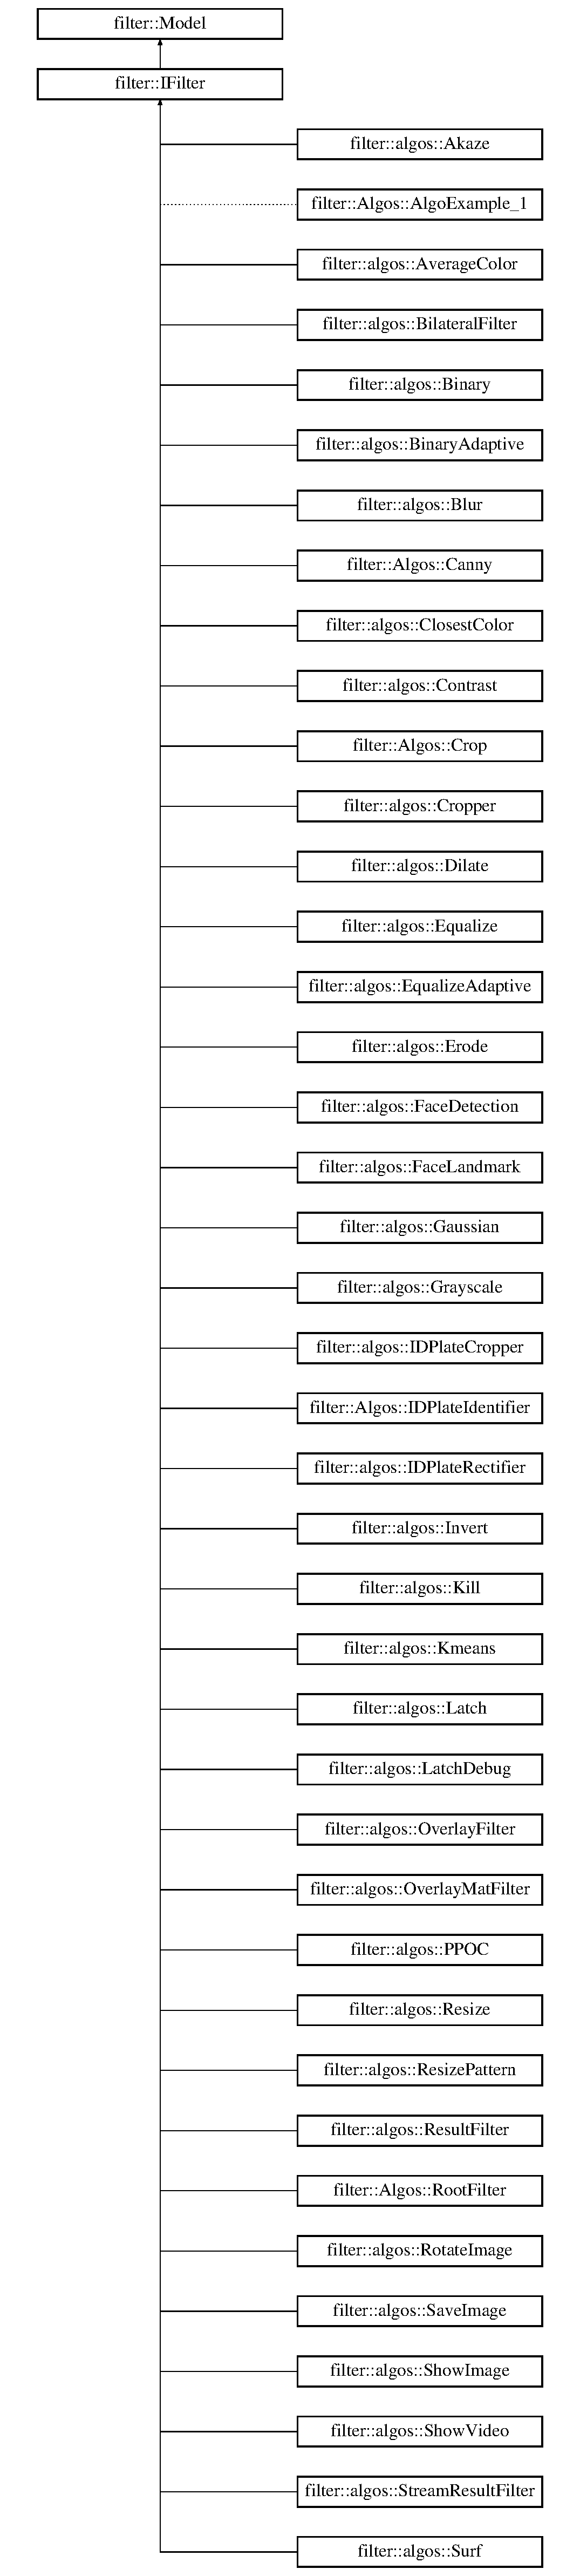
\includegraphics[height=12.000000cm]{d4/d8a/classfilter_1_1_i_filter}
\end{center}
\end{figure}
\subsection*{Public Member Functions}
\begin{DoxyCompactItemize}
\item 
\mbox{\Hypertarget{classfilter_1_1_i_filter_acc2eda7686fb753d4fdc76d7c7cb7fe9}\label{classfilter_1_1_i_filter_acc2eda7686fb753d4fdc76d7c7cb7fe9}} 
{\bfseries I\+Filter} (std\+::string contructor\+Name)
\item 
\mbox{\Hypertarget{classfilter_1_1_i_filter_a1ba2261bc75ed3e23ec9b14fd78661de}\label{classfilter_1_1_i_filter_a1ba2261bc75ed3e23ec9b14fd78661de}} 
virtual void {\bfseries get\+Next\+Filter} ()
\item 
\mbox{\Hypertarget{classfilter_1_1_i_filter_a46f7e69f03ccf1d3227dddcb2ff5edd7}\label{classfilter_1_1_i_filter_a46f7e69f03ccf1d3227dddcb2ff5edd7}} 
virtual void {\bfseries get\+Previous\+Filter} ()
\item 
virtual \hyperlink{classfilter_1_1_i_filter}{I\+Filter} $\ast$ \hyperlink{classfilter_1_1_i_filter_a97fdc1892c15c918287c83263d069147}{get\+Root\+Filter} ()
\begin{DoxyCompactList}\small\item\em Get the Root\+Filter node (head) of the current graph. \end{DoxyCompactList}\item 
\mbox{\Hypertarget{classfilter_1_1_i_filter_ab4a3bdc9a1e04edd8f1cedb2fc51b234}\label{classfilter_1_1_i_filter_ab4a3bdc9a1e04edd8f1cedb2fc51b234}} 
virtual void {\bfseries get\+Parent} ()
\item 
\mbox{\Hypertarget{classfilter_1_1_i_filter_a9c6127d9371057896377e07c73fe9de2}\label{classfilter_1_1_i_filter_a9c6127d9371057896377e07c73fe9de2}} 
virtual void {\bfseries get\+Next\+Children} ()
\item 
virtual std\+::string \hyperlink{classfilter_1_1_i_filter_ab99902b060a6d9edc3452a8c9f85e37e}{result\+As\+String} ()
\begin{DoxyCompactList}\small\item\em Get the result of the processing done by the node. This method will return information only. The actual processing is done by the process() method. \end{DoxyCompactList}\item 
virtual void \hyperlink{classfilter_1_1_i_filter_a3132d332ce814fda5c1a17a3e498c4fb}{add\+Dependencies} (\hyperlink{classfilter_1_1_model}{Model} $\ast$filter)
\begin{DoxyCompactList}\small\item\em Create a parent child dependency between two filters. Every parent will be processed before its child. \end{DoxyCompactList}\item 
\mbox{\Hypertarget{classfilter_1_1_i_filter_a49c161e0e74bc8169a47c5832adc80bf}\label{classfilter_1_1_i_filter_a49c161e0e74bc8169a47c5832adc80bf}} 
virtual void {\bfseries add\+Child\+Dependencies} (\hyperlink{classfilter_1_1_model}{Model} $\ast$filter)
\item 
\mbox{\Hypertarget{classfilter_1_1_i_filter_a342b79ca87a0a80cdc9283f791445a5d}\label{classfilter_1_1_i_filter_a342b79ca87a0a80cdc9283f791445a5d}} 
virtual void {\bfseries add\+Dependencies\+Name} (std\+::string filter)
\item 
\mbox{\Hypertarget{classfilter_1_1_i_filter_adad5caef656f6e03875e9370821af953}\label{classfilter_1_1_i_filter_adad5caef656f6e03875e9370821af953}} 
virtual void {\bfseries add\+Child\+Dependencies\+Name} (std\+::string filter)
\item 
\mbox{\Hypertarget{classfilter_1_1_i_filter_a5573a79109562b2bce0ef402f016b62b}\label{classfilter_1_1_i_filter_a5573a79109562b2bce0ef402f016b62b}} 
virtual std\+::map$<$ std\+::string, \hyperlink{classfilter_1_1_model}{Model} $\ast$ $>$ {\bfseries get\+Parents} () const
\item 
\mbox{\Hypertarget{classfilter_1_1_i_filter_aa4473ecc2a050e587982915958d58591}\label{classfilter_1_1_i_filter_aa4473ecc2a050e587982915958d58591}} 
virtual std\+::map$<$ std\+::string, \hyperlink{classfilter_1_1_model}{Model} $\ast$ $>$ {\bfseries get\+Childrens} () const
\item 
\mbox{\Hypertarget{classfilter_1_1_i_filter_ae1eb446deaca10fec8882e22c401f3c3}\label{classfilter_1_1_i_filter_ae1eb446deaca10fec8882e22c401f3c3}} 
virtual \hyperlink{classfilter_1_1_i_filter}{I\+Filter} \& {\bfseries operator$<$$<$} (\hyperlink{classfilter_1_1data_1_1_data}{data\+::\+Data} \&element)
\item 
\mbox{\Hypertarget{classfilter_1_1_i_filter_aab026b67b2b7d0675c3c840a7d19a1d4}\label{classfilter_1_1_i_filter_aab026b67b2b7d0675c3c840a7d19a1d4}} 
virtual \hyperlink{classfilter_1_1_i_filter}{I\+Filter} \& {\bfseries operator$<$$<$} (cv\+::\+Mat \&element)
\item 
\mbox{\Hypertarget{classfilter_1_1_i_filter_acfdd4ae98b9915471dc7990d2d8bce62}\label{classfilter_1_1_i_filter_acfdd4ae98b9915471dc7990d2d8bce62}} 
virtual \hyperlink{classfilter_1_1_i_filter}{I\+Filter} \& {\bfseries get\+Cast} ()
\item 
\mbox{\Hypertarget{classfilter_1_1_i_filter_a9a683f58c2b38861f84a71185b7042a1}\label{classfilter_1_1_i_filter_a9a683f58c2b38861f84a71185b7042a1}} 
virtual \hyperlink{classfilter_1_1_i_filter}{I\+Filter} \& {\bfseries operator$<$$<$} (\hyperlink{classfilter_1_1_i_filter}{I\+Filter} \&other)
\item 
\mbox{\Hypertarget{classfilter_1_1_i_filter_afce54ff6662fa18ebfa5a17d6a915b87}\label{classfilter_1_1_i_filter_afce54ff6662fa18ebfa5a17d6a915b87}} 
virtual \hyperlink{classfilter_1_1data_1_1_connex_data_base}{data\+::\+Connex\+Data\+Base} \& {\bfseries get\+Connector} ()
\item 
\mbox{\Hypertarget{classfilter_1_1_i_filter_a62fe91f40b01cb886e923d8073392348}\label{classfilter_1_1_i_filter_a62fe91f40b01cb886e923d8073392348}} 
virtual Hipe\+Status {\bfseries process} ()=0
\end{DoxyCompactItemize}
\subsection*{Protected Attributes}
\begin{DoxyCompactItemize}
\item 
\mbox{\Hypertarget{classfilter_1_1_i_filter_a8fb81acc82a39393799f3d3e29861be2}\label{classfilter_1_1_i_filter_a8fb81acc82a39393799f3d3e29861be2}} 
std\+::map$<$ std\+::string, \hyperlink{classfilter_1_1_model}{Model} $\ast$ $>$ {\bfseries \+\_\+parent\+Filters}
\item 
\mbox{\Hypertarget{classfilter_1_1_i_filter_a4408ce375b706fb8e809417fccb4dbfe}\label{classfilter_1_1_i_filter_a4408ce375b706fb8e809417fccb4dbfe}} 
std\+::map$<$ std\+::string, \hyperlink{classfilter_1_1_model}{Model} $\ast$ $>$ {\bfseries \+\_\+child\+Filters}
\end{DoxyCompactItemize}


\subsection{Detailed Description}
\begin{DoxyRefDesc}{Todo}
\item[\hyperlink{todo__todo000027}{Todo}]\end{DoxyRefDesc}


\subsection{Member Function Documentation}
\mbox{\Hypertarget{classfilter_1_1_i_filter_a3132d332ce814fda5c1a17a3e498c4fb}\label{classfilter_1_1_i_filter_a3132d332ce814fda5c1a17a3e498c4fb}} 
\index{filter\+::\+I\+Filter@{filter\+::\+I\+Filter}!add\+Dependencies@{add\+Dependencies}}
\index{add\+Dependencies@{add\+Dependencies}!filter\+::\+I\+Filter@{filter\+::\+I\+Filter}}
\subsubsection{\texorpdfstring{add\+Dependencies()}{addDependencies()}}
{\footnotesize\ttfamily void filter\+::\+I\+Filter\+::add\+Dependencies (\begin{DoxyParamCaption}\item[{\hyperlink{classfilter_1_1_model}{Model} $\ast$}]{filter }\end{DoxyParamCaption})\hspace{0.3cm}{\ttfamily [virtual]}}


\begin{DoxyParams}{Parameters}
{\em filter} & The filter to add as dependency \\
\hline
\end{DoxyParams}


Implements \hyperlink{classfilter_1_1_model}{filter\+::\+Model}.

\mbox{\Hypertarget{classfilter_1_1_i_filter_a97fdc1892c15c918287c83263d069147}\label{classfilter_1_1_i_filter_a97fdc1892c15c918287c83263d069147}} 
\index{filter\+::\+I\+Filter@{filter\+::\+I\+Filter}!get\+Root\+Filter@{get\+Root\+Filter}}
\index{get\+Root\+Filter@{get\+Root\+Filter}!filter\+::\+I\+Filter@{filter\+::\+I\+Filter}}
\subsubsection{\texorpdfstring{get\+Root\+Filter()}{getRootFilter()}}
{\footnotesize\ttfamily \hyperlink{classfilter_1_1_i_filter}{filter\+::\+I\+Filter} $\ast$ filter\+::\+I\+Filter\+::get\+Root\+Filter (\begin{DoxyParamCaption}{ }\end{DoxyParamCaption})\hspace{0.3cm}{\ttfamily [virtual]}}

\begin{DoxyReturn}{Returns}
A pointer to the Root\+Filter node of the graph 
\end{DoxyReturn}


Implements \hyperlink{classfilter_1_1_model}{filter\+::\+Model}.

\mbox{\Hypertarget{classfilter_1_1_i_filter_ab99902b060a6d9edc3452a8c9f85e37e}\label{classfilter_1_1_i_filter_ab99902b060a6d9edc3452a8c9f85e37e}} 
\index{filter\+::\+I\+Filter@{filter\+::\+I\+Filter}!result\+As\+String@{result\+As\+String}}
\index{result\+As\+String@{result\+As\+String}!filter\+::\+I\+Filter@{filter\+::\+I\+Filter}}
\subsubsection{\texorpdfstring{result\+As\+String()}{resultAsString()}}
{\footnotesize\ttfamily virtual std\+::string filter\+::\+I\+Filter\+::result\+As\+String (\begin{DoxyParamCaption}{ }\end{DoxyParamCaption})\hspace{0.3cm}{\ttfamily [inline]}, {\ttfamily [virtual]}}

\begin{DoxyReturn}{Returns}
A string containing the result of the processing done by the filter. 
\end{DoxyReturn}


Reimplemented in \hyperlink{classfilter_1_1_algos_1_1_crop_a44ded08379421eb046be865a884139e8}{filter\+::\+Algos\+::\+Crop}, \hyperlink{classfilter_1_1algos_1_1_cropper_ae970d5d448587b8288aca2484f12f2fa}{filter\+::algos\+::\+Cropper}, \hyperlink{classfilter_1_1algos_1_1_latch_a24c57b8d90c89b1f95fe2f7624a9d033}{filter\+::algos\+::\+Latch}, \hyperlink{classfilter_1_1algos_1_1_stream_result_filter_acdd774d7dc6a7b807d5fc0bfe3343949}{filter\+::algos\+::\+Stream\+Result\+Filter}, \hyperlink{classfilter_1_1algos_1_1_face_detection_a11c5004107d5048de93ae81ced065a26}{filter\+::algos\+::\+Face\+Detection}, \hyperlink{classfilter_1_1algos_1_1_face_landmark_a58eca9d87717bac1696c2b008af4342a}{filter\+::algos\+::\+Face\+Landmark}, \hyperlink{classfilter_1_1algos_1_1_show_image_a752acc552a91b93b42acf0a1269b5e73}{filter\+::algos\+::\+Show\+Image}, \hyperlink{classfilter_1_1algos_1_1_show_video_a8fc9113fbd7f9648ea0997304ca91aec}{filter\+::algos\+::\+Show\+Video}, \hyperlink{classfilter_1_1algos_1_1_resize_a5f4bc6f31fd5d759f1216ce60b1358b0}{filter\+::algos\+::\+Resize}, \hyperlink{classfilter_1_1algos_1_1_akaze_afbbbf680eb0c14ea7e47dbc78169f32b}{filter\+::algos\+::\+Akaze}, \hyperlink{classfilter_1_1algos_1_1_kmeans_aed99c18aeec39add2955b2b9b3361a8a}{filter\+::algos\+::\+Kmeans}, \hyperlink{classfilter_1_1algos_1_1_rotate_image_af9aeff9c2232e6fc97708cbc41ee1fb2}{filter\+::algos\+::\+Rotate\+Image}, \hyperlink{classfilter_1_1algos_1_1_overlay_filter_ac591ab39d8e08ccfe8f96020e438958d}{filter\+::algos\+::\+Overlay\+Filter}, \hyperlink{classfilter_1_1algos_1_1_surf_ad7aae2eb2e5a5f2a0277eb5d58153833}{filter\+::algos\+::\+Surf}, \hyperlink{classfilter_1_1algos_1_1_overlay_mat_filter_a819c132897fd3a1e4f4f28378313ccdd}{filter\+::algos\+::\+Overlay\+Mat\+Filter}, \hyperlink{classfilter_1_1algos_1_1_resize_pattern_ae36ff1d98ef8f2dd32ba5b7a3a50152f}{filter\+::algos\+::\+Resize\+Pattern}, \hyperlink{classfilter_1_1algos_1_1_kill_af12b57f54905370350c6a7f291f99a6c}{filter\+::algos\+::\+Kill}, \hyperlink{classfilter_1_1algos_1_1_result_filter_a0a67e26005d8b32a69fb6e6bec80788c}{filter\+::algos\+::\+Result\+Filter}, and \hyperlink{classfilter_1_1algos_1_1_gaussian_a5f2ba86fa61807781b46fe321e435c29}{filter\+::algos\+::\+Gaussian}.



The documentation for this class was generated from the following files\+:\begin{DoxyCompactItemize}
\item 
header/filter/I\+Filter.\+h\item 
source/filter/I\+Filter.\+cpp\end{DoxyCompactItemize}

\hypertarget{classhttp_1_1_server_base_1_1_request_1_1ihash}{}\section{http\+:\+:Server\+Base$<$ socket\+\_\+type $>$\+:\+:Request\+:\+:ihash Class Reference}
\label{classhttp_1_1_server_base_1_1_request_1_1ihash}\index{http\+::\+Server\+Base$<$ socket\+\_\+type $>$\+::\+Request\+::ihash@{http\+::\+Server\+Base$<$ socket\+\_\+type $>$\+::\+Request\+::ihash}}
\subsection*{Public Member Functions}
\begin{DoxyCompactItemize}
\item 
\mbox{\Hypertarget{classhttp_1_1_server_base_1_1_request_1_1ihash_afdb9199e93314c528b6c7cd9a8186228}\label{classhttp_1_1_server_base_1_1_request_1_1ihash_afdb9199e93314c528b6c7cd9a8186228}} 
size\+\_\+t {\bfseries operator()} (const std\+::string \&key) const
\end{DoxyCompactItemize}


The documentation for this class was generated from the following file\+:\begin{DoxyCompactItemize}
\item 
header/http/Http\+Server.\+hpp\end{DoxyCompactItemize}

\hypertarget{classhttp_1_1_request_1_1ihash}{}\section{http\+:\+:Request$<$ socket\+\_\+type $>$\+:\+:ihash Class Reference}
\label{classhttp_1_1_request_1_1ihash}\index{http\+::\+Request$<$ socket\+\_\+type $>$\+::ihash@{http\+::\+Request$<$ socket\+\_\+type $>$\+::ihash}}
\subsection*{Public Member Functions}
\begin{DoxyCompactItemize}
\item 
\mbox{\Hypertarget{classhttp_1_1_request_1_1ihash_acd9c30d020432330b333afde0aff0a70}\label{classhttp_1_1_request_1_1ihash_acd9c30d020432330b333afde0aff0a70}} 
size\+\_\+t {\bfseries operator()} (const std\+::string \&key) const
\end{DoxyCompactItemize}


The documentation for this class was generated from the following file\+:\begin{DoxyCompactItemize}
\item 
header/http/Request.\+h\end{DoxyCompactItemize}

\hypertarget{classhttp_1_1_client_base_1_1_response_1_1ihash}{}\section{http\+:\+:Client\+Base$<$ socket\+\_\+type $>$\+:\+:Response\+:\+:ihash Class Reference}
\label{classhttp_1_1_client_base_1_1_response_1_1ihash}\index{http\+::\+Client\+Base$<$ socket\+\_\+type $>$\+::\+Response\+::ihash@{http\+::\+Client\+Base$<$ socket\+\_\+type $>$\+::\+Response\+::ihash}}
\subsection*{Public Member Functions}
\begin{DoxyCompactItemize}
\item 
\mbox{\Hypertarget{classhttp_1_1_client_base_1_1_response_1_1ihash_aabba60d960eb1ca18468e2a0d647c98e}\label{classhttp_1_1_client_base_1_1_response_1_1ihash_aabba60d960eb1ca18468e2a0d647c98e}} 
size\+\_\+t {\bfseries operator()} (const std\+::string \&key) const
\end{DoxyCompactItemize}


The documentation for this class was generated from the following file\+:\begin{DoxyCompactItemize}
\item 
header/http/Http\+Client.\+h\end{DoxyCompactItemize}

\hypertarget{classfilter_1_1data_1_1_image_array_data}{}\section{filter\+:\+:data\+:\+:Image\+Array\+Data Class Reference}
\label{classfilter_1_1data_1_1_image_array_data}\index{filter\+::data\+::\+Image\+Array\+Data@{filter\+::data\+::\+Image\+Array\+Data}}


\hyperlink{classfilter_1_1data_1_1_image_array_data}{Image\+Array\+Data} is the data type used to handle multiple images. Uses Open\+CV.  




{\ttfamily \#include $<$Image\+Array\+Data.\+h$>$}

Inheritance diagram for filter\+:\+:data\+:\+:Image\+Array\+Data\+:\begin{figure}[H]
\begin{center}
\leavevmode
\includegraphics[height=3.809524cm]{d6/d44/classfilter_1_1data_1_1_image_array_data}
\end{center}
\end{figure}
\subsection*{Public Member Functions}
\begin{DoxyCompactItemize}
\item 
\mbox{\Hypertarget{classfilter_1_1data_1_1_image_array_data_a410e2084318c82c3ed886a467757b027}\label{classfilter_1_1data_1_1_image_array_data_a410e2084318c82c3ed886a467757b027}} 
\hyperlink{classfilter_1_1data_1_1_image_array_data_a410e2084318c82c3ed886a467757b027}{Image\+Array\+Data} ()
\begin{DoxyCompactList}\small\item\em \hyperlink{classfilter_1_1data_1_1_image_array_data}{Image\+Array\+Data} default constructor, the internal I\+O\+Data\+Type data type will be \char`\"{}\+S\+E\+Q\+I\+M\+G\char`\"{}. \end{DoxyCompactList}\item 
\hyperlink{classfilter_1_1data_1_1_image_array_data_aaaf37db86b4659ac8cb10e5f44a2869b}{Image\+Array\+Data} (const \hyperlink{classfilter_1_1data_1_1_image_array_data}{data\+::\+Image\+Array\+Data} \&right)
\begin{DoxyCompactList}\small\item\em \hyperlink{classfilter_1_1data_1_1_image_array_data}{Image\+Array\+Data} copy constructor. \end{DoxyCompactList}\item 
std\+::vector$<$ cv\+::\+Mat $>$ \& \hyperlink{classfilter_1_1data_1_1_image_array_data_acded510f22f9c549adea6174e44dae2a}{Array} ()
\begin{DoxyCompactList}\small\item\em Get the container of the images\textquotesingle{} data. \end{DoxyCompactList}\item 
const std\+::vector$<$ cv\+::\+Mat $>$ \& \hyperlink{classfilter_1_1data_1_1_image_array_data_a5bc06808faaf76e0cbbb5944788cef79}{Array\+\_\+const} () const
\begin{DoxyCompactList}\small\item\em Get the container of the images\textquotesingle{} data (const version) \end{DoxyCompactList}\item 
\hyperlink{classfilter_1_1data_1_1_image_array_data}{Image\+Array\+Data} \& \hyperlink{classfilter_1_1data_1_1_image_array_data_a43e4ed2752d0ae2a1685d1f52adcebde}{operator$<$$<$} (cv\+::\+Mat data\+Mat)
\begin{DoxyCompactList}\small\item\em Add an image to the container. \end{DoxyCompactList}\item 
virtual void \hyperlink{classfilter_1_1data_1_1_image_array_data_abc051d3a4e57bdb5a3ee47e35df6ea9d}{copy\+To} (\hyperlink{classfilter_1_1data_1_1_image_array_data}{Image\+Array\+Data} \&left) const
\begin{DoxyCompactList}\small\item\em Copy the images\textquotesingle{} data of the \hyperlink{classfilter_1_1data_1_1_image_array_data}{Image\+Array\+Data} object to another one. \end{DoxyCompactList}\item 
bool \hyperlink{classfilter_1_1data_1_1_image_array_data_ac30c0a0384b1133a8c177e399ff9d140}{empty} () const
\item 
\hyperlink{classfilter_1_1data_1_1_image_array_data}{Image\+Array\+Data} \& \hyperlink{classfilter_1_1data_1_1_image_array_data_a6986bd7246e4468bf9afd2c2196608fc}{operator=} (const \hyperlink{classfilter_1_1data_1_1_image_array_data}{Image\+Array\+Data} \&left)
\begin{DoxyCompactList}\small\item\em \hyperlink{classfilter_1_1data_1_1_image_array_data}{Image\+Array\+Data} assignment operator. \end{DoxyCompactList}\end{DoxyCompactItemize}
\subsection*{Protected Member Functions}
\begin{DoxyCompactItemize}
\item 
\mbox{\Hypertarget{classfilter_1_1data_1_1_image_array_data_ac5dce50dc7e25871855e6c86bce18925}\label{classfilter_1_1data_1_1_image_array_data_ac5dce50dc7e25871855e6c86bce18925}} 
{\bfseries Image\+Array\+Data} (data\+::\+I\+O\+Data\+Type type)
\end{DoxyCompactItemize}
\subsection*{Protected Attributes}
\begin{DoxyCompactItemize}
\item 
\mbox{\Hypertarget{classfilter_1_1data_1_1_image_array_data_ab46da947b17f81791d8b59038780b2cd}\label{classfilter_1_1data_1_1_image_array_data_ab46da947b17f81791d8b59038780b2cd}} 
std\+::vector$<$ cv\+::\+Mat $>$ {\bfseries \+\_\+array}
\end{DoxyCompactItemize}
\subsection*{Additional Inherited Members}


\subsection{Constructor \& Destructor Documentation}
\mbox{\Hypertarget{classfilter_1_1data_1_1_image_array_data_aaaf37db86b4659ac8cb10e5f44a2869b}\label{classfilter_1_1data_1_1_image_array_data_aaaf37db86b4659ac8cb10e5f44a2869b}} 
\index{filter\+::data\+::\+Image\+Array\+Data@{filter\+::data\+::\+Image\+Array\+Data}!Image\+Array\+Data@{Image\+Array\+Data}}
\index{Image\+Array\+Data@{Image\+Array\+Data}!filter\+::data\+::\+Image\+Array\+Data@{filter\+::data\+::\+Image\+Array\+Data}}
\subsubsection{\texorpdfstring{Image\+Array\+Data()}{ImageArrayData()}}
{\footnotesize\ttfamily filter\+::data\+::\+Image\+Array\+Data\+::\+Image\+Array\+Data (\begin{DoxyParamCaption}\item[{const \hyperlink{classfilter_1_1data_1_1_image_array_data}{data\+::\+Image\+Array\+Data} \&}]{right }\end{DoxyParamCaption})\hspace{0.3cm}{\ttfamily [inline]}}


\begin{DoxyParams}{Parameters}
{\em right} & The \hyperlink{classfilter_1_1data_1_1_image_array_data}{Image\+Array\+Data} to copy data from \\
\hline
\end{DoxyParams}


\subsection{Member Function Documentation}
\mbox{\Hypertarget{classfilter_1_1data_1_1_image_array_data_acded510f22f9c549adea6174e44dae2a}\label{classfilter_1_1data_1_1_image_array_data_acded510f22f9c549adea6174e44dae2a}} 
\index{filter\+::data\+::\+Image\+Array\+Data@{filter\+::data\+::\+Image\+Array\+Data}!Array@{Array}}
\index{Array@{Array}!filter\+::data\+::\+Image\+Array\+Data@{filter\+::data\+::\+Image\+Array\+Data}}
\subsubsection{\texorpdfstring{Array()}{Array()}}
{\footnotesize\ttfamily std\+::vector$<$cv\+::\+Mat$>$\& filter\+::data\+::\+Image\+Array\+Data\+::\+Array (\begin{DoxyParamCaption}{ }\end{DoxyParamCaption})\hspace{0.3cm}{\ttfamily [inline]}}

\begin{DoxyReturn}{Returns}
Returns a reference to the std\+::vector$<$cv\+::\+Mat$>$ object containing the images\textquotesingle{} data 
\end{DoxyReturn}
\mbox{\Hypertarget{classfilter_1_1data_1_1_image_array_data_a5bc06808faaf76e0cbbb5944788cef79}\label{classfilter_1_1data_1_1_image_array_data_a5bc06808faaf76e0cbbb5944788cef79}} 
\index{filter\+::data\+::\+Image\+Array\+Data@{filter\+::data\+::\+Image\+Array\+Data}!Array\+\_\+const@{Array\+\_\+const}}
\index{Array\+\_\+const@{Array\+\_\+const}!filter\+::data\+::\+Image\+Array\+Data@{filter\+::data\+::\+Image\+Array\+Data}}
\subsubsection{\texorpdfstring{Array\+\_\+const()}{Array\_const()}}
{\footnotesize\ttfamily const std\+::vector$<$cv\+::\+Mat$>$\& filter\+::data\+::\+Image\+Array\+Data\+::\+Array\+\_\+const (\begin{DoxyParamCaption}{ }\end{DoxyParamCaption}) const\hspace{0.3cm}{\ttfamily [inline]}}

\begin{DoxyReturn}{Returns}
Returns a constant reference to the std\+::vector$<$cv\+::\+Mat$>$ object containing the images\textquotesingle{} data 
\end{DoxyReturn}
\mbox{\Hypertarget{classfilter_1_1data_1_1_image_array_data_abc051d3a4e57bdb5a3ee47e35df6ea9d}\label{classfilter_1_1data_1_1_image_array_data_abc051d3a4e57bdb5a3ee47e35df6ea9d}} 
\index{filter\+::data\+::\+Image\+Array\+Data@{filter\+::data\+::\+Image\+Array\+Data}!copy\+To@{copy\+To}}
\index{copy\+To@{copy\+To}!filter\+::data\+::\+Image\+Array\+Data@{filter\+::data\+::\+Image\+Array\+Data}}
\subsubsection{\texorpdfstring{copy\+To()}{copyTo()}}
{\footnotesize\ttfamily virtual void filter\+::data\+::\+Image\+Array\+Data\+::copy\+To (\begin{DoxyParamCaption}\item[{\hyperlink{classfilter_1_1data_1_1_image_array_data}{Image\+Array\+Data} \&}]{left }\end{DoxyParamCaption}) const\hspace{0.3cm}{\ttfamily [inline]}, {\ttfamily [virtual]}}


\begin{DoxyParams}{Parameters}
{\em left} & The other object where to copy the data to \\
\hline
\end{DoxyParams}
\mbox{\Hypertarget{classfilter_1_1data_1_1_image_array_data_ac30c0a0384b1133a8c177e399ff9d140}\label{classfilter_1_1data_1_1_image_array_data_ac30c0a0384b1133a8c177e399ff9d140}} 
\index{filter\+::data\+::\+Image\+Array\+Data@{filter\+::data\+::\+Image\+Array\+Data}!empty@{empty}}
\index{empty@{empty}!filter\+::data\+::\+Image\+Array\+Data@{filter\+::data\+::\+Image\+Array\+Data}}
\subsubsection{\texorpdfstring{empty()}{empty()}}
{\footnotesize\ttfamily bool filter\+::data\+::\+Image\+Array\+Data\+::empty (\begin{DoxyParamCaption}{ }\end{DoxyParamCaption}) const\hspace{0.3cm}{\ttfamily [inline]}, {\ttfamily [virtual]}}

\begin{DoxyReturn}{Returns}
Returns true if the object doesn\textquotesingle{}t contain any data 
\end{DoxyReturn}


Reimplemented from \hyperlink{classfilter_1_1data_1_1_i_o_data}{filter\+::data\+::\+I\+O\+Data$<$ Data, Image\+Array\+Data $>$}.



Reimplemented in \hyperlink{classfilter_1_1data_1_1_image_data_aa2aa6922b9cad5746a16a66e15665717}{filter\+::data\+::\+Image\+Data}.

\mbox{\Hypertarget{classfilter_1_1data_1_1_image_array_data_a43e4ed2752d0ae2a1685d1f52adcebde}\label{classfilter_1_1data_1_1_image_array_data_a43e4ed2752d0ae2a1685d1f52adcebde}} 
\index{filter\+::data\+::\+Image\+Array\+Data@{filter\+::data\+::\+Image\+Array\+Data}!operator$<$$<$@{operator$<$$<$}}
\index{operator$<$$<$@{operator$<$$<$}!filter\+::data\+::\+Image\+Array\+Data@{filter\+::data\+::\+Image\+Array\+Data}}
\subsubsection{\texorpdfstring{operator$<$$<$()}{operator<<()}}
{\footnotesize\ttfamily \hyperlink{classfilter_1_1data_1_1_image_array_data}{Image\+Array\+Data}\& filter\+::data\+::\+Image\+Array\+Data\+::operator$<$$<$ (\begin{DoxyParamCaption}\item[{cv\+::\+Mat}]{data\+Mat }\end{DoxyParamCaption})\hspace{0.3cm}{\ttfamily [inline]}}


\begin{DoxyParams}{Parameters}
{\em data\+Mat} & The image to add \\
\hline
\end{DoxyParams}
\begin{DoxyReturn}{Returns}
Returns a reference to the \hyperlink{classfilter_1_1data_1_1_image_array_data}{Image\+Array\+Data} object 
\end{DoxyReturn}
\mbox{\Hypertarget{classfilter_1_1data_1_1_image_array_data_a6986bd7246e4468bf9afd2c2196608fc}\label{classfilter_1_1data_1_1_image_array_data_a6986bd7246e4468bf9afd2c2196608fc}} 
\index{filter\+::data\+::\+Image\+Array\+Data@{filter\+::data\+::\+Image\+Array\+Data}!operator=@{operator=}}
\index{operator=@{operator=}!filter\+::data\+::\+Image\+Array\+Data@{filter\+::data\+::\+Image\+Array\+Data}}
\subsubsection{\texorpdfstring{operator=()}{operator=()}}
{\footnotesize\ttfamily \hyperlink{classfilter_1_1data_1_1_image_array_data}{Image\+Array\+Data}\& filter\+::data\+::\+Image\+Array\+Data\+::operator= (\begin{DoxyParamCaption}\item[{const \hyperlink{classfilter_1_1data_1_1_image_array_data}{Image\+Array\+Data} \&}]{left }\end{DoxyParamCaption})\hspace{0.3cm}{\ttfamily [inline]}}

\begin{DoxyRefDesc}{Todo}
\item[\hyperlink{todo__todo000022}{Todo}]\end{DoxyRefDesc}

\begin{DoxyParams}{Parameters}
{\em left} & The \hyperlink{classfilter_1_1data_1_1_image_array_data}{Image\+Array\+Data} oject to get the data from \\
\hline
\end{DoxyParams}
\begin{DoxyReturn}{Returns}
A reference to the object 
\end{DoxyReturn}


The documentation for this class was generated from the following file\+:\begin{DoxyCompactItemize}
\item 
header/filter/data/Image\+Array\+Data.\+h\end{DoxyCompactItemize}

\hypertarget{classfilter_1_1data_1_1_image_data}{}\section{filter\+:\+:data\+:\+:Image\+Data Class Reference}
\label{classfilter_1_1data_1_1_image_data}\index{filter\+::data\+::\+Image\+Data@{filter\+::data\+::\+Image\+Data}}


\hyperlink{classfilter_1_1data_1_1_image_data}{Image\+Data} is the data type used to handle an image. Uses Open\+CV.  




{\ttfamily \#include $<$Image\+Data.\+h$>$}

Inheritance diagram for filter\+:\+:data\+:\+:Image\+Data\+:\begin{figure}[H]
\begin{center}
\leavevmode
\includegraphics[height=7.000000cm]{db/dbc/classfilter_1_1data_1_1_image_data}
\end{center}
\end{figure}
\subsection*{Public Member Functions}
\begin{DoxyCompactItemize}
\item 
\mbox{\Hypertarget{classfilter_1_1data_1_1_image_data_abb536d27922733a27037118802ab6191}\label{classfilter_1_1data_1_1_image_data_abb536d27922733a27037118802ab6191}} 
\hyperlink{classfilter_1_1data_1_1_image_data_abb536d27922733a27037118802ab6191}{Image\+Data} ()
\begin{DoxyCompactList}\small\item\em Default empty constructor. \end{DoxyCompactList}\item 
\hyperlink{classfilter_1_1data_1_1_image_data_ae34694d9ed284c8c85d4a67a52f09f12}{Image\+Data} (cv\+::\+Mat matrix)
\item 
\mbox{\Hypertarget{classfilter_1_1data_1_1_image_data_ad62a19517fe97ec50c3cc55b30c7096f}\label{classfilter_1_1data_1_1_image_data_ad62a19517fe97ec50c3cc55b30c7096f}} 
{\bfseries Image\+Data} (const \hyperlink{classfilter_1_1data_1_1_image_data}{Image\+Data} \&ref)
\item 
virtual void \hyperlink{classfilter_1_1data_1_1_image_data_ab035bfe80f8f6a6470046eb15fad7dfb}{copy\+To} (\hyperlink{classfilter_1_1data_1_1_image_data}{Image\+Data} \&left) const
\begin{DoxyCompactList}\small\item\em Copy the image data of the \hyperlink{classfilter_1_1data_1_1_image_data}{Image\+Data} object to another one. \end{DoxyCompactList}\item 
cv\+::\+Mat \& \hyperlink{classfilter_1_1data_1_1_image_data_aed944725082cbf0ab8def1af23612917}{get\+Mat} ()
\begin{DoxyCompactList}\small\item\em Get the image\textquotesingle{}s data. \end{DoxyCompactList}\item 
const cv\+::\+Mat \& \hyperlink{classfilter_1_1data_1_1_image_data_abccbb6bc292443ba7772febadd6e4884}{get\+Mat} () const
\begin{DoxyCompactList}\small\item\em Get the image\textquotesingle{}s data (const version) \end{DoxyCompactList}\item 
bool \hyperlink{classfilter_1_1data_1_1_image_data_aa2aa6922b9cad5746a16a66e15665717}{empty} () const
\item 
\mbox{\Hypertarget{classfilter_1_1data_1_1_image_data_a98f56c3e6c8738b72c91c0a082ae74ef}\label{classfilter_1_1data_1_1_image_data_a98f56c3e6c8738b72c91c0a082ae74ef}} 
\hyperlink{classfilter_1_1data_1_1_image_data}{Image\+Data} \& {\bfseries operator=} (const \hyperlink{classfilter_1_1data_1_1_data}{Data} \&left)
\end{DoxyCompactItemize}
\subsection*{Protected Member Functions}
\begin{DoxyCompactItemize}
\item 
\mbox{\Hypertarget{classfilter_1_1data_1_1_image_data_aa1a881853016f3ce06d3fdeac8e3a875}\label{classfilter_1_1data_1_1_image_data_aa1a881853016f3ce06d3fdeac8e3a875}} 
{\bfseries Image\+Data} (\hyperlink{classfilter_1_1data_1_1_i_o_data_1_1___protection}{I\+O\+Data\+::\+\_\+\+Protection} priv)
\item 
\mbox{\Hypertarget{classfilter_1_1data_1_1_image_data_a3e56635b65d792a87554d635c8b20d1e}\label{classfilter_1_1data_1_1_image_data_a3e56635b65d792a87554d635c8b20d1e}} 
{\bfseries Image\+Data} (I\+O\+Data\+Type data\+Type)
\end{DoxyCompactItemize}
\subsection*{Additional Inherited Members}


\subsection{Constructor \& Destructor Documentation}
\mbox{\Hypertarget{classfilter_1_1data_1_1_image_data_ae34694d9ed284c8c85d4a67a52f09f12}\label{classfilter_1_1data_1_1_image_data_ae34694d9ed284c8c85d4a67a52f09f12}} 
\index{filter\+::data\+::\+Image\+Data@{filter\+::data\+::\+Image\+Data}!Image\+Data@{Image\+Data}}
\index{Image\+Data@{Image\+Data}!filter\+::data\+::\+Image\+Data@{filter\+::data\+::\+Image\+Data}}
\subsubsection{\texorpdfstring{Image\+Data()}{ImageData()}}
{\footnotesize\ttfamily filter\+::data\+::\+Image\+Data\+::\+Image\+Data (\begin{DoxyParamCaption}\item[{cv\+::\+Mat}]{matrix }\end{DoxyParamCaption})\hspace{0.3cm}{\ttfamily [inline]}}


\begin{DoxyParams}{Parameters}
{\em matrix} & The image\textquotesingle{}s data \\
\hline
\end{DoxyParams}


\subsection{Member Function Documentation}
\mbox{\Hypertarget{classfilter_1_1data_1_1_image_data_ab035bfe80f8f6a6470046eb15fad7dfb}\label{classfilter_1_1data_1_1_image_data_ab035bfe80f8f6a6470046eb15fad7dfb}} 
\index{filter\+::data\+::\+Image\+Data@{filter\+::data\+::\+Image\+Data}!copy\+To@{copy\+To}}
\index{copy\+To@{copy\+To}!filter\+::data\+::\+Image\+Data@{filter\+::data\+::\+Image\+Data}}
\subsubsection{\texorpdfstring{copy\+To()}{copyTo()}}
{\footnotesize\ttfamily virtual void filter\+::data\+::\+Image\+Data\+::copy\+To (\begin{DoxyParamCaption}\item[{\hyperlink{classfilter_1_1data_1_1_image_data}{Image\+Data} \&}]{left }\end{DoxyParamCaption}) const\hspace{0.3cm}{\ttfamily [inline]}, {\ttfamily [virtual]}}


\begin{DoxyParams}{Parameters}
{\em left} & The object where to copy the data to \\
\hline
\end{DoxyParams}


Reimplemented in \hyperlink{classfilter_1_1data_1_1_file_image_data_a188f2f5ab66877f6ba553cc847cd5f07}{filter\+::data\+::\+File\+Image\+Data}.

\mbox{\Hypertarget{classfilter_1_1data_1_1_image_data_aa2aa6922b9cad5746a16a66e15665717}\label{classfilter_1_1data_1_1_image_data_aa2aa6922b9cad5746a16a66e15665717}} 
\index{filter\+::data\+::\+Image\+Data@{filter\+::data\+::\+Image\+Data}!empty@{empty}}
\index{empty@{empty}!filter\+::data\+::\+Image\+Data@{filter\+::data\+::\+Image\+Data}}
\subsubsection{\texorpdfstring{empty()}{empty()}}
{\footnotesize\ttfamily bool filter\+::data\+::\+Image\+Data\+::empty (\begin{DoxyParamCaption}{ }\end{DoxyParamCaption}) const\hspace{0.3cm}{\ttfamily [inline]}, {\ttfamily [virtual]}}

\begin{DoxyReturn}{Returns}
Returns true if the object doesn\textquotesingle{}t contain any data 
\end{DoxyReturn}


Reimplemented from \hyperlink{classfilter_1_1data_1_1_i_o_data}{filter\+::data\+::\+I\+O\+Data$<$ Image\+Array\+Data, Image\+Data $>$}.

\mbox{\Hypertarget{classfilter_1_1data_1_1_image_data_aed944725082cbf0ab8def1af23612917}\label{classfilter_1_1data_1_1_image_data_aed944725082cbf0ab8def1af23612917}} 
\index{filter\+::data\+::\+Image\+Data@{filter\+::data\+::\+Image\+Data}!get\+Mat@{get\+Mat}}
\index{get\+Mat@{get\+Mat}!filter\+::data\+::\+Image\+Data@{filter\+::data\+::\+Image\+Data}}
\subsubsection{\texorpdfstring{get\+Mat()}{getMat()}\hspace{0.1cm}{\footnotesize\ttfamily [1/2]}}
{\footnotesize\ttfamily cv\+::\+Mat\& filter\+::data\+::\+Image\+Data\+::get\+Mat (\begin{DoxyParamCaption}{ }\end{DoxyParamCaption})\hspace{0.3cm}{\ttfamily [inline]}}

\begin{DoxyReturn}{Returns}
Returns a reference to the cv\+::\+Mat object containing the image\textquotesingle{}s data 
\end{DoxyReturn}
\mbox{\Hypertarget{classfilter_1_1data_1_1_image_data_abccbb6bc292443ba7772febadd6e4884}\label{classfilter_1_1data_1_1_image_data_abccbb6bc292443ba7772febadd6e4884}} 
\index{filter\+::data\+::\+Image\+Data@{filter\+::data\+::\+Image\+Data}!get\+Mat@{get\+Mat}}
\index{get\+Mat@{get\+Mat}!filter\+::data\+::\+Image\+Data@{filter\+::data\+::\+Image\+Data}}
\subsubsection{\texorpdfstring{get\+Mat()}{getMat()}\hspace{0.1cm}{\footnotesize\ttfamily [2/2]}}
{\footnotesize\ttfamily const cv\+::\+Mat\& filter\+::data\+::\+Image\+Data\+::get\+Mat (\begin{DoxyParamCaption}{ }\end{DoxyParamCaption}) const\hspace{0.3cm}{\ttfamily [inline]}}

\begin{DoxyReturn}{Returns}
Returns a constant reference to the cv\+::\+Mat object containing the image\textquotesingle{}s data 
\end{DoxyReturn}


The documentation for this class was generated from the following file\+:\begin{DoxyCompactItemize}
\item 
header/filter/data/Image\+Data.\+h\end{DoxyCompactItemize}

\hypertarget{classfilter_1_1algos_1_1_invert}{}\section{filter\+:\+:algos\+:\+:Invert Class Reference}
\label{classfilter_1_1algos_1_1_invert}\index{filter\+::algos\+::\+Invert@{filter\+::algos\+::\+Invert}}


The \hyperlink{classfilter_1_1algos_1_1_invert}{Invert} filter will invert the colors of an image.  




{\ttfamily \#include $<$Invert.\+h$>$}

Inheritance diagram for filter\+:\+:algos\+:\+:Invert\+:\begin{figure}[H]
\begin{center}
\leavevmode
\includegraphics[height=3.000000cm]{d5/d93/classfilter_1_1algos_1_1_invert}
\end{center}
\end{figure}
\subsection*{Public Types}
\begin{DoxyCompactItemize}
\item 
\mbox{\Hypertarget{classfilter_1_1algos_1_1_invert_ad4bfea474f67af264fa18ac0c360fdbf}\label{classfilter_1_1algos_1_1_invert_ad4bfea474f67af264fa18ac0c360fdbf}} 
typedef \hyperlink{class_proxy_functor}{Proxy\+Functor}$<$ \hyperlink{classfilter_1_1algos_1_1_invert}{Invert} $>$ {\bfseries \+\_\+proxy\+Functor}
\item 
\mbox{\Hypertarget{classfilter_1_1algos_1_1_invert_aaeb1c627d08a1e5e6cdbcefc108ec4dc}\label{classfilter_1_1algos_1_1_invert_aaeb1c627d08a1e5e6cdbcefc108ec4dc}} 
typedef \hyperlink{classfilter_1_1algos_1_1_invert}{Invert} {\bfseries mytype}
\item 
\mbox{\Hypertarget{classfilter_1_1algos_1_1_invert_acc0c44d84876a788db4f9704b99649b4}\label{classfilter_1_1algos_1_1_invert_acc0c44d84876a788db4f9704b99649b4}} 
typedef char {\bfseries vartype\+\_\+\+\_\+unused}
\end{DoxyCompactItemize}
\subsection*{Public Member Functions}
\begin{DoxyCompactItemize}
\item 
\mbox{\Hypertarget{classfilter_1_1algos_1_1_invert_a5e764405ca99c9684f35fb7e30231658}\label{classfilter_1_1algos_1_1_invert_a5e764405ca99c9684f35fb7e30231658}} 
void {\bfseries set\+\_\+unused\+\_\+from\+\_\+json} (boost\+::property\+\_\+tree\+::ptree \&json\+Class)
\item 
\mbox{\Hypertarget{classfilter_1_1algos_1_1_invert_aa528c0fa98d4afe5b092156c48f1bd92}\label{classfilter_1_1algos_1_1_invert_aa528c0fa98d4afe5b092156c48f1bd92}} 
void {\bfseries set\+\_\+unused} (vartype\+\_\+\+\_\+unused \&\+\_\+\+\_\+unused)
\item 
\mbox{\Hypertarget{classfilter_1_1algos_1_1_invert_a55ef1bc3577c561fdea1287ae09747c3}\label{classfilter_1_1algos_1_1_invert_a55ef1bc3577c561fdea1287ae09747c3}} 
vartype\+\_\+\+\_\+unused {\bfseries get\+\_\+unused} ()
\item 
\mbox{\Hypertarget{classfilter_1_1algos_1_1_invert_af8d2c83ed933c5dda102a17bc592b480}\label{classfilter_1_1algos_1_1_invert_af8d2c83ed933c5dda102a17bc592b480}} 
void {\bfseries copy\+\_\+unused} (\hyperlink{classfilter_1_1algos_1_1_invert}{mytype} $\ast$instance)
\item 
\mbox{\Hypertarget{classfilter_1_1algos_1_1_invert_a7da6240f7b961067c8da807553378777}\label{classfilter_1_1algos_1_1_invert_a7da6240f7b961067c8da807553378777}} 
Hipe\+Status {\bfseries process} () override
\end{DoxyCompactItemize}
\subsection*{Public Attributes}
\begin{DoxyCompactItemize}
\item 
\mbox{\Hypertarget{classfilter_1_1algos_1_1_invert_abb7caf9e273cbb371e52dd4ccbf01be6}\label{classfilter_1_1algos_1_1_invert_abb7caf9e273cbb371e52dd4ccbf01be6}} 
char {\bfseries unused}
\end{DoxyCompactItemize}
\subsection*{Private Member Functions}
\begin{DoxyCompactItemize}
\item 
\mbox{\Hypertarget{classfilter_1_1algos_1_1_invert_a2716f9a946dd23a21dddc840b2e7730e}\label{classfilter_1_1algos_1_1_invert_a2716f9a946dd23a21dddc840b2e7730e}} 
virtual \hyperlink{classfilter_1_1data_1_1_connex_data_base}{data\+::\+Connex\+Data\+Base} \& {\bfseries get\+Connector} ()
\end{DoxyCompactItemize}
\subsection*{Private Attributes}
\begin{DoxyCompactItemize}
\item 
\mbox{\Hypertarget{classfilter_1_1algos_1_1_invert_adde7147440d10f9d4e9cb171f84389c6}\label{classfilter_1_1algos_1_1_invert_adde7147440d10f9d4e9cb171f84389c6}} 
\hyperlink{classfilter_1_1data_1_1_connex_data}{data\+::\+Connex\+Data}$<$ \hyperlink{classfilter_1_1data_1_1_image_data}{data\+::\+Image\+Data}, \hyperlink{classfilter_1_1data_1_1_image_data}{data\+::\+Image\+Data} $>$ {\bfseries \+\_\+connex\+Data}
\end{DoxyCompactItemize}
\subsection*{Additional Inherited Members}


The documentation for this class was generated from the following file\+:\begin{DoxyCompactItemize}
\item 
header/filter/\+Algos/Invert.\+h\end{DoxyCompactItemize}

\hypertarget{classcore_1_1_invoker}{}\section{core\+:\+:Invoker$<$ return\+\_\+type, params $>$ Class Template Reference}
\label{classcore_1_1_invoker}\index{core\+::\+Invoker$<$ return\+\_\+type, params $>$@{core\+::\+Invoker$<$ return\+\_\+type, params $>$}}
Inheritance diagram for core\+:\+:Invoker$<$ return\+\_\+type, params $>$\+:\begin{figure}[H]
\begin{center}
\leavevmode
\includegraphics[height=2.000000cm]{d3/dca/classcore_1_1_invoker}
\end{center}
\end{figure}
\subsection*{Classes}
\begin{DoxyCompactItemize}
\item 
struct \hyperlink{structcore_1_1_invoker_1_1_wrapper}{Wrapper}
\end{DoxyCompactItemize}
\subsection*{Public Member Functions}
\begin{DoxyCompactItemize}
\item 
\mbox{\Hypertarget{classcore_1_1_invoker_a7a061acd788cce09e236b5d88c81539d}\label{classcore_1_1_invoker_a7a061acd788cce09e236b5d88c81539d}} 
{\bfseries Invoker} (Type function)
\item 
\mbox{\Hypertarget{classcore_1_1_invoker_af11a95ae72d36ca19d104211ebd9b14b}\label{classcore_1_1_invoker_af11a95ae72d36ca19d104211ebd9b14b}} 
{\bfseries Invoker} (\hyperlink{classcore_1_1_invoker}{Invoker} \&right)
\item 
\mbox{\Hypertarget{classcore_1_1_invoker_a6c299259795abe41fffe3af74d1189a3}\label{classcore_1_1_invoker_a6c299259795abe41fffe3af74d1189a3}} 
void {\bfseries operator=} (\hyperlink{classcore_1_1_invoker}{Invoker} \&right)
\item 
\mbox{\Hypertarget{classcore_1_1_invoker_a77880ac54daebaf9c7845b51decc3de6}\label{classcore_1_1_invoker_a77880ac54daebaf9c7845b51decc3de6}} 
return\+\_\+type {\bfseries operator()} (void $\ast$callee, params... xs)
\end{DoxyCompactItemize}
\subsection*{Static Public Member Functions}
\begin{DoxyCompactItemize}
\item 
\mbox{\Hypertarget{classcore_1_1_invoker_a3bd0db4d50a571274962ef1d52f00470}\label{classcore_1_1_invoker_a3bd0db4d50a571274962ef1d52f00470}} 
{\footnotesize template$<$class T , return\+\_\+type(\+T\+::$\ast$)(params...) T\+Method$>$ }\\static \hyperlink{classcore_1_1_invoker}{Invoker}$<$ return\+\_\+type, params... $>$ {\bfseries for\+\_\+function} ()
\end{DoxyCompactItemize}
\subsection*{Private Types}
\begin{DoxyCompactItemize}
\item 
\mbox{\Hypertarget{classcore_1_1_invoker_afa39d69cc0b13c031e7bc852fcf6c823}\label{classcore_1_1_invoker_afa39d69cc0b13c031e7bc852fcf6c823}} 
typedef return\+\_\+type($\ast$ {\bfseries Type}) (void $\ast$callee, params...)
\end{DoxyCompactItemize}
\subsection*{Static Private Member Functions}
\begin{DoxyCompactItemize}
\item 
\mbox{\Hypertarget{classcore_1_1_invoker_ac3a4c67c5938fe9d38b28bbfe4451ef5}\label{classcore_1_1_invoker_ac3a4c67c5938fe9d38b28bbfe4451ef5}} 
{\footnotesize template$<$class T , return\+\_\+type(\+T\+::$\ast$)(params...) T\+Method$>$ }\\static return\+\_\+type {\bfseries method\+Invoke} (void $\ast$callee, params... xs)
\end{DoxyCompactItemize}
\subsection*{Additional Inherited Members}


The documentation for this class was generated from the following file\+:\begin{DoxyCompactItemize}
\item 
header/core/Invoker.\+h\end{DoxyCompactItemize}

\hypertarget{classcore_1_1_invoker_base}{}\section{core\+:\+:Invoker\+Base Class Reference}
\label{classcore_1_1_invoker_base}\index{core\+::\+Invoker\+Base@{core\+::\+Invoker\+Base}}
Inheritance diagram for core\+:\+:Invoker\+Base\+:\begin{figure}[H]
\begin{center}
\leavevmode
\includegraphics[height=2.000000cm]{d9/d1c/classcore_1_1_invoker_base}
\end{center}
\end{figure}
\subsection*{Classes}
\begin{DoxyCompactItemize}
\item 
struct \hyperlink{structcore_1_1_invoker_base_1_1_wrapper_base}{Wrapper\+Base}
\end{DoxyCompactItemize}
\subsection*{Public Member Functions}
\begin{DoxyCompactItemize}
\item 
\mbox{\Hypertarget{classcore_1_1_invoker_base_acaa5cea166578cc7bba04ae395168004}\label{classcore_1_1_invoker_base_acaa5cea166578cc7bba04ae395168004}} 
{\bfseries Invoker\+Base} (\hyperlink{classcore_1_1_invoker_base}{Invoker\+Base} \&invo\+Method)
\item 
\mbox{\Hypertarget{classcore_1_1_invoker_base_a4af10eb6aef42a0544fd53c9d57b6b6c}\label{classcore_1_1_invoker_base_a4af10eb6aef42a0544fd53c9d57b6b6c}} 
{\bfseries Invoker\+Base} (const \hyperlink{classcore_1_1_invoker_base}{Invoker\+Base} \&invo\+Method)
\item 
\mbox{\Hypertarget{classcore_1_1_invoker_base_a087544175e041a38cf15684d7eb2f23f}\label{classcore_1_1_invoker_base_a087544175e041a38cf15684d7eb2f23f}} 
{\footnotesize template$<$typename return\+\_\+type , typename... params$>$ }\\\hyperlink{classcore_1_1_invoker_base}{Invoker\+Base} \& {\bfseries operator=} (\hyperlink{classcore_1_1_invoker}{Invoker}$<$ return\+\_\+type, params... $>$ invo\+Method)
\item 
\mbox{\Hypertarget{classcore_1_1_invoker_base_afc7fa6502d4297140cf8ab3408479c63}\label{classcore_1_1_invoker_base_afc7fa6502d4297140cf8ab3408479c63}} 
{\footnotesize template$<$typename return\+\_\+type , typename... params$>$ }\\return\+\_\+type {\bfseries operator()} (void $\ast$callee, params... xs)
\item 
\mbox{\Hypertarget{classcore_1_1_invoker_base_a2186a47cae984d9e43d3f2f7d2632301}\label{classcore_1_1_invoker_base_a2186a47cae984d9e43d3f2f7d2632301}} 
{\footnotesize template$<$typename return\+\_\+type , typename... params$>$ }\\\hyperlink{classcore_1_1_invoker}{Invoker}$<$ return\+\_\+type, params... $>$ \& {\bfseries operator=} (const \hyperlink{classcore_1_1_invoker}{Invoker}$<$ return\+\_\+type, params... $>$ \&invo\+Method)
\item 
\mbox{\Hypertarget{classcore_1_1_invoker_base_a20d2a080ce9e7cb6a4b200179db33efd}\label{classcore_1_1_invoker_base_a20d2a080ce9e7cb6a4b200179db33efd}} 
{\footnotesize template$<$typename return\+\_\+type , typename... params$>$ }\\\hyperlink{classcore_1_1_invoker}{Invoker}$<$ return\+\_\+type, params... $>$ \& {\bfseries operator=} (\hyperlink{classcore_1_1_invoker}{Invoker}$<$ return\+\_\+type, params... $>$ invo\+Method)
\item 
\mbox{\Hypertarget{classcore_1_1_invoker_base_a218efa44504723e111ac82841445514e}\label{classcore_1_1_invoker_base_a218efa44504723e111ac82841445514e}} 
\hyperlink{classcore_1_1_invoker_base}{Invoker\+Base} \& {\bfseries operator=} (const \hyperlink{classcore_1_1_invoker_base}{Invoker\+Base} \&invo\+Method)
\end{DoxyCompactItemize}
\subsection*{Protected Attributes}
\begin{DoxyCompactItemize}
\item 
\mbox{\Hypertarget{classcore_1_1_invoker_base_aac1eb2d0482d5c4897b8abb3aa93dc64}\label{classcore_1_1_invoker_base_aac1eb2d0482d5c4897b8abb3aa93dc64}} 
std\+::unique\+\_\+ptr$<$ \hyperlink{structcore_1_1_invoker_base_1_1_wrapper_base}{Wrapper\+Base} $>$ {\bfseries \+\_\+wrap}
\end{DoxyCompactItemize}


The documentation for this class was generated from the following file\+:\begin{DoxyCompactItemize}
\item 
header/core/Invoker.\+h\end{DoxyCompactItemize}

\hypertarget{classfilter_1_1data_1_1_i_o_data}{}\section{filter\+:\+:data\+:\+:I\+O\+Data$<$ Base, Derived $>$ Class Template Reference}
\label{classfilter_1_1data_1_1_i_o_data}\index{filter\+::data\+::\+I\+O\+Data$<$ Base, Derived $>$@{filter\+::data\+::\+I\+O\+Data$<$ Base, Derived $>$}}


\mbox{[}T\+O\+DO\mbox{]}  




{\ttfamily \#include $<$I\+O\+Data.\+h$>$}

Inheritance diagram for filter\+:\+:data\+:\+:I\+O\+Data$<$ Base, Derived $>$\+:\begin{figure}[H]
\begin{center}
\leavevmode
\includegraphics[height=2.000000cm]{d0/d51/classfilter_1_1data_1_1_i_o_data}
\end{center}
\end{figure}
\subsection*{Classes}
\begin{DoxyCompactItemize}
\item 
class \hyperlink{classfilter_1_1data_1_1_i_o_data_1_1___protection}{\+\_\+\+Protection}
\end{DoxyCompactItemize}
\subsection*{Public Member Functions}
\begin{DoxyCompactItemize}
\item 
\mbox{\Hypertarget{classfilter_1_1data_1_1_i_o_data_a2598b5a08dcfbc4e5d003bdb10dbfe2f}\label{classfilter_1_1data_1_1_i_o_data_a2598b5a08dcfbc4e5d003bdb10dbfe2f}} 
{\bfseries I\+O\+Data} (const Base \&base)
\item 
\mbox{\Hypertarget{classfilter_1_1data_1_1_i_o_data_a4520de80fec35f20b190dfc627be85b7}\label{classfilter_1_1data_1_1_i_o_data_a4520de80fec35f20b190dfc627be85b7}} 
void {\bfseries release} ()
\item 
virtual void \hyperlink{classfilter_1_1data_1_1_i_o_data_a6ad82e2b326a0f436391225daa728458}{copy\+To} (\hyperlink{classfilter_1_1data_1_1_i_o_data}{I\+O\+Data} \&left) const
\begin{DoxyCompactList}\small\item\em Depracated to review no way to copy on left if it\textquotesingle{}s const .... \end{DoxyCompactList}\item 
\mbox{\Hypertarget{classfilter_1_1data_1_1_i_o_data_ad946eec587df7e314385d2dbeb26b7bf}\label{classfilter_1_1data_1_1_i_o_data_ad946eec587df7e314385d2dbeb26b7bf}} 
virtual bool {\bfseries empty} () const
\item 
\mbox{\Hypertarget{classfilter_1_1data_1_1_i_o_data_a5fd8e6c021ce4e02c724443ad6551bde}\label{classfilter_1_1data_1_1_i_o_data_a5fd8e6c021ce4e02c724443ad6551bde}} 
I\+O\+Data\+Type {\bfseries get\+Type} () const
\item 
\mbox{\Hypertarget{classfilter_1_1data_1_1_i_o_data_affc92e9fdd4d0a058720991df9b7fb90}\label{classfilter_1_1data_1_1_i_o_data_affc92e9fdd4d0a058720991df9b7fb90}} 
const Derived \& {\bfseries This\+\_\+const} () const
\item 
\mbox{\Hypertarget{classfilter_1_1data_1_1_i_o_data_a4356d2768be576818fbcb0e1bb059d4b}\label{classfilter_1_1data_1_1_i_o_data_a4356d2768be576818fbcb0e1bb059d4b}} 
Derived \& {\bfseries This} ()
\item 
\mbox{\Hypertarget{classfilter_1_1data_1_1_i_o_data_a98a5ee1a06a79df6b60e79d5769688df}\label{classfilter_1_1data_1_1_i_o_data_a98a5ee1a06a79df6b60e79d5769688df}} 
Derived \& {\bfseries operator=} (const \hyperlink{classfilter_1_1data_1_1_data}{Data} \&left)
\end{DoxyCompactItemize}


\subsection{Detailed Description}
\subsubsection*{template$<$typename Base, typename Derived$>$\newline
class filter\+::data\+::\+I\+O\+Data$<$ Base, Derived $>$}

\begin{DoxyRefDesc}{Todo}
\item[\hyperlink{todo__todo000024}{Todo}]\end{DoxyRefDesc}

\begin{DoxyTemplParams}{Template Parameters}
{\em Base} & \\
\hline
{\em Derived} & \\
\hline
\end{DoxyTemplParams}


\subsection{Member Function Documentation}
\mbox{\Hypertarget{classfilter_1_1data_1_1_i_o_data_a6ad82e2b326a0f436391225daa728458}\label{classfilter_1_1data_1_1_i_o_data_a6ad82e2b326a0f436391225daa728458}} 
\index{filter\+::data\+::\+I\+O\+Data@{filter\+::data\+::\+I\+O\+Data}!copy\+To@{copy\+To}}
\index{copy\+To@{copy\+To}!filter\+::data\+::\+I\+O\+Data@{filter\+::data\+::\+I\+O\+Data}}
\subsubsection{\texorpdfstring{copy\+To()}{copyTo()}}
{\footnotesize\ttfamily template$<$typename Base, typename Derived$>$ \\
virtual void \hyperlink{classfilter_1_1data_1_1_i_o_data}{filter\+::data\+::\+I\+O\+Data}$<$ Base, Derived $>$\+::copy\+To (\begin{DoxyParamCaption}\item[{\hyperlink{classfilter_1_1data_1_1_i_o_data}{I\+O\+Data}$<$ Base, Derived $>$ \&}]{left }\end{DoxyParamCaption}) const\hspace{0.3cm}{\ttfamily [inline]}, {\ttfamily [virtual]}}


\begin{DoxyParams}{Parameters}
{\em left} & \\
\hline
\end{DoxyParams}


Reimplemented in \hyperlink{classfilter_1_1data_1_1_i_o_data_a6ad82e2b326a0f436391225daa728458}{filter\+::data\+::\+I\+O\+Data$<$ Image\+Array\+Data, Image\+Data $>$}, \hyperlink{classfilter_1_1data_1_1_i_o_data_a6ad82e2b326a0f436391225daa728458}{filter\+::data\+::\+I\+O\+Data$<$ Image\+Array\+Data, Output\+Data $>$}, \hyperlink{classfilter_1_1data_1_1_i_o_data_a6ad82e2b326a0f436391225daa728458}{filter\+::data\+::\+I\+O\+Data$<$ Image\+Array\+Data, Directory\+Img\+Data $>$}, and \hyperlink{classfilter_1_1data_1_1_i_o_data_a6ad82e2b326a0f436391225daa728458}{filter\+::data\+::\+I\+O\+Data$<$ Image\+Data, File\+Image\+Data $>$}.



The documentation for this class was generated from the following file\+:\begin{DoxyCompactItemize}
\item 
header/filter/data/I\+O\+Data.\+h\end{DoxyCompactItemize}

\hypertarget{classfilter_1_1algos_1_1_i_p_desc}{}\section{filter\+:\+:algos\+:\+:I\+P\+Desc Class Reference}
\label{classfilter_1_1algos_1_1_i_p_desc}\index{filter\+::algos\+::\+I\+P\+Desc@{filter\+::algos\+::\+I\+P\+Desc}}
\subsection*{Public Member Functions}
\begin{DoxyCompactItemize}
\item 
\mbox{\Hypertarget{classfilter_1_1algos_1_1_i_p_desc_a338b99191d2c6d113f5066ee6eb4fb2c}\label{classfilter_1_1algos_1_1_i_p_desc_a338b99191d2c6d113f5066ee6eb4fb2c}} 
{\bfseries I\+P\+Desc} (cv\+::\+Mat object, int pointX, int pointY, int point\+Width, int point\+Height)
\item 
\mbox{\Hypertarget{classfilter_1_1algos_1_1_i_p_desc_a77658ad6f018aa44ec183829ad09e8d9}\label{classfilter_1_1algos_1_1_i_p_desc_a77658ad6f018aa44ec183829ad09e8d9}} 
cv\+::\+Point {\bfseries corner} () const
\item 
\mbox{\Hypertarget{classfilter_1_1algos_1_1_i_p_desc_a31c5f7d3d96b7dc8282b9235303c3fee}\label{classfilter_1_1algos_1_1_i_p_desc_a31c5f7d3d96b7dc8282b9235303c3fee}} 
cv\+::\+Rect {\bfseries rect} () const
\item 
\mbox{\Hypertarget{classfilter_1_1algos_1_1_i_p_desc_a4288a962e862ed4f195cece5dee195de}\label{classfilter_1_1algos_1_1_i_p_desc_a4288a962e862ed4f195cece5dee195de}} 
int {\bfseries width} () const
\item 
\mbox{\Hypertarget{classfilter_1_1algos_1_1_i_p_desc_a496bab19b6b7bad8cbdf68f91315ba2d}\label{classfilter_1_1algos_1_1_i_p_desc_a496bab19b6b7bad8cbdf68f91315ba2d}} 
int {\bfseries height} () const
\item 
\mbox{\Hypertarget{classfilter_1_1algos_1_1_i_p_desc_aacb1e157aa650ad40e38b7179e256ce4}\label{classfilter_1_1algos_1_1_i_p_desc_aacb1e157aa650ad40e38b7179e256ce4}} 
cv\+::\+Mat {\bfseries desc\+Img} () const
\end{DoxyCompactItemize}
\subsection*{Private Attributes}
\begin{DoxyCompactItemize}
\item 
\mbox{\Hypertarget{classfilter_1_1algos_1_1_i_p_desc_a07ee01efcc59d57830508dcd92ec0602}\label{classfilter_1_1algos_1_1_i_p_desc_a07ee01efcc59d57830508dcd92ec0602}} 
cv\+::\+Rect {\bfseries corner\+\_\+}
\item 
\mbox{\Hypertarget{classfilter_1_1algos_1_1_i_p_desc_a84b26d0f28a676142bf9f561d066d99e}\label{classfilter_1_1algos_1_1_i_p_desc_a84b26d0f28a676142bf9f561d066d99e}} 
cv\+::\+Mat {\bfseries desc\+Img\+\_\+}
\end{DoxyCompactItemize}


The documentation for this class was generated from the following file\+:\begin{DoxyCompactItemize}
\item 
header/filter/\+Algos/P\+P\+O\+C.\+h\end{DoxyCompactItemize}

\hypertarget{classjson_1_1_json_builder}{}\section{json\+:\+:Json\+Builder Class Reference}
\label{classjson_1_1_json_builder}\index{json\+::\+Json\+Builder@{json\+::\+Json\+Builder}}
\subsection*{Static Public Member Functions}
\begin{DoxyCompactItemize}
\item 
\mbox{\Hypertarget{classjson_1_1_json_builder_a61ed78182f56e5a6f105164d4dd8d36a}\label{classjson_1_1_json_builder_a61ed78182f56e5a6f105164d4dd8d36a}} 
static \hyperlink{classjson_1_1_json_filter_tree}{json\+::\+Json\+Filter\+Tree} $\ast$ {\bfseries build\+Algorithm} (std\+::stringstream \&data\+Response, boost\+::property\+\_\+tree\+::ptree \&tree\+Request)
\item 
\mbox{\Hypertarget{classjson_1_1_json_builder_ad94b8ff719a5321d058e8e8472fd6443}\label{classjson_1_1_json_builder_ad94b8ff719a5321d058e8e8472fd6443}} 
static std\+::string {\bfseries get\+Or\+Build\+Orchestrator} (std\+::stringstream \&data\+\_\+response, boost\+::property\+\_\+tree\+::ptree \&tree\+Request)
\end{DoxyCompactItemize}


The documentation for this class was generated from the following files\+:\begin{DoxyCompactItemize}
\item 
header/json/Json\+Builder.\+h\item 
source/json/Json\+Builder.\+cpp\end{DoxyCompactItemize}

\hypertarget{classjson_1_1_json_filter_node}{}\section{json\+:\+:Json\+Filter\+Node Class Reference}
\label{classjson_1_1_json_filter_node}\index{json\+::\+Json\+Filter\+Node@{json\+::\+Json\+Filter\+Node}}
\subsection*{Public Member Functions}
\begin{DoxyCompactItemize}
\item 
\mbox{\Hypertarget{classjson_1_1_json_filter_node_a9df5d3a1c9309fbc3f59bf7929b504f0}\label{classjson_1_1_json_filter_node_a9df5d3a1c9309fbc3f59bf7929b504f0}} 
std\+::vector$<$ std\+::string $>$ {\bfseries get\+Dependencies\+Filter} ()
\item 
\mbox{\Hypertarget{classjson_1_1_json_filter_node_a7ed12a9049b701ecab0485f572fd4703}\label{classjson_1_1_json_filter_node_a7ed12a9049b701ecab0485f572fd4703}} 
{\bfseries Json\+Filter\+Node} (\hyperlink{classfilter_1_1_model}{filter\+::\+Model} $\ast$filter, boost\+::property\+\_\+tree\+::ptree \&params)
\item 
\mbox{\Hypertarget{classjson_1_1_json_filter_node_a251b7ce3ae1aa2f32c34571271f5c3d4}\label{classjson_1_1_json_filter_node_a251b7ce3ae1aa2f32c34571271f5c3d4}} 
void {\bfseries apply\+Class\+Parameter} ()
\item 
\mbox{\Hypertarget{classjson_1_1_json_filter_node_aa06d4f8ac48c5c39c6708ac84e04fd7b}\label{classjson_1_1_json_filter_node_aa06d4f8ac48c5c39c6708ac84e04fd7b}} 
\hyperlink{classfilter_1_1_model}{filter\+::\+Model} $\ast$ {\bfseries get\+Filter} ()
\end{DoxyCompactItemize}
\subsection*{Static Public Member Functions}
\begin{DoxyCompactItemize}
\item 
\mbox{\Hypertarget{classjson_1_1_json_filter_node_acdcd269942e402495740a6b84eeca26c}\label{classjson_1_1_json_filter_node_acdcd269942e402495740a6b84eeca26c}} 
{\footnotesize template$<$typename T $>$ }\\static std\+::vector$<$ T $>$ {\bfseries as\+\_\+vector} (boost\+::property\+\_\+tree\+::ptree const \&pt, boost\+::property\+\_\+tree\+::ptree\+::key\+\_\+type const \&key)
\end{DoxyCompactItemize}
\subsection*{Private Attributes}
\begin{DoxyCompactItemize}
\item 
\mbox{\Hypertarget{classjson_1_1_json_filter_node_a82a2c12454ba06b0574c83165399017e}\label{classjson_1_1_json_filter_node_a82a2c12454ba06b0574c83165399017e}} 
\hyperlink{classfilter_1_1_model}{filter\+::\+Model} $\ast$ {\bfseries \+\_\+filter}
\item 
\mbox{\Hypertarget{classjson_1_1_json_filter_node_a587e67fff551bff400221ae6fe88b7af}\label{classjson_1_1_json_filter_node_a587e67fff551bff400221ae6fe88b7af}} 
boost\+::property\+\_\+tree\+::ptree \& {\bfseries \+\_\+params}
\end{DoxyCompactItemize}


The documentation for this class was generated from the following file\+:\begin{DoxyCompactItemize}
\item 
header/json/\+Json\+Filter\+Node/Json\+Filter\+Node.\+h\end{DoxyCompactItemize}

\hypertarget{classjson_1_1_json_filter_tree}{}\section{json\+:\+:Json\+Filter\+Tree Class Reference}
\label{classjson_1_1_json_filter_tree}\index{json\+::\+Json\+Filter\+Tree@{json\+::\+Json\+Filter\+Tree}}
Inheritance diagram for json\+:\+:Json\+Filter\+Tree\+:\begin{figure}[H]
\begin{center}
\leavevmode
\includegraphics[height=2.000000cm]{d9/d9b/classjson_1_1_json_filter_tree}
\end{center}
\end{figure}
\subsection*{Public Member Functions}
\begin{DoxyCompactItemize}
\item 
\mbox{\Hypertarget{classjson_1_1_json_filter_tree_aa7819d6838b8046ff3906ea6bd6fa66f}\label{classjson_1_1_json_filter_tree_aa7819d6838b8046ff3906ea6bd6fa66f}} 
{\bfseries Json\+Filter\+Tree} (const \hyperlink{classjson_1_1_json_filter_tree}{Json\+Filter\+Tree} \&j\+Tree)
\item 
\mbox{\Hypertarget{classjson_1_1_json_filter_tree_ad1ec96718c7c454d4e3f19ba8d43146e}\label{classjson_1_1_json_filter_tree_ad1ec96718c7c454d4e3f19ba8d43146e}} 
void {\bfseries freeze} ()
\item 
void \hyperlink{classjson_1_1_json_filter_tree_aee36fd03a671233001426a3c6657f0f8}{add} (\hyperlink{classjson_1_1_json_filter_node}{Json\+Filter\+Node} \&filter\+Node)
\item 
\mbox{\Hypertarget{classjson_1_1_json_filter_tree_a4ed24b965ae9071fccb678f3567b3aea}\label{classjson_1_1_json_filter_tree_a4ed24b965ae9071fccb678f3567b3aea}} 
void {\bfseries compute\+Link\+Dependencies} ()
\item 
\mbox{\Hypertarget{classjson_1_1_json_filter_tree_a005fdda47cd93ffb7531d0985f75bb42}\label{classjson_1_1_json_filter_tree_a005fdda47cd93ffb7531d0985f75bb42}} 
void {\bfseries compute\+Level\+Node} ()
\item 
\mbox{\Hypertarget{classjson_1_1_json_filter_tree_a467aa6119f119a25ed71dd786d8850fa}\label{classjson_1_1_json_filter_tree_a467aa6119f119a25ed71dd786d8850fa}} 
\hyperlink{classfilter_1_1_model}{filter\+::\+Model} $\ast$ {\bfseries get\+Root\+Node} ()
\item 
\mbox{\Hypertarget{classjson_1_1_json_filter_tree_ab7ad587899cfa6a5ae76e3bc4ca2234f}\label{classjson_1_1_json_filter_tree_ab7ad587899cfa6a5ae76e3bc4ca2234f}} 
void {\bfseries add\+Dependencies} (Model $\ast$filter) override
\item 
\mbox{\Hypertarget{classjson_1_1_json_filter_tree_af65e7e183cfe7cab7b2529fa34579fd6}\label{classjson_1_1_json_filter_tree_af65e7e183cfe7cab7b2529fa34579fd6}} 
void {\bfseries add\+Child\+Dependencies} (Model $\ast$filter) override
\item 
\mbox{\Hypertarget{classjson_1_1_json_filter_tree_af6301cab0669da01d7cd75f3468dc4a7}\label{classjson_1_1_json_filter_tree_af6301cab0669da01d7cd75f3468dc4a7}} 
void {\bfseries add\+Dependencies\+Name} (std\+::string filter) override
\item 
\mbox{\Hypertarget{classjson_1_1_json_filter_tree_a5d2806db27fed87671d81edd42d2b115}\label{classjson_1_1_json_filter_tree_a5d2806db27fed87671d81edd42d2b115}} 
void {\bfseries add\+Child\+Dependencies\+Name} (std\+::string filter) override
\item 
\mbox{\Hypertarget{classjson_1_1_json_filter_tree_a44e9e49893a0e6ec05f9ca6aec75bef1}\label{classjson_1_1_json_filter_tree_a44e9e49893a0e6ec05f9ca6aec75bef1}} 
std\+::map$<$ std\+::string, Model $\ast$ $>$ {\bfseries get\+Parents} () const override
\item 
\mbox{\Hypertarget{classjson_1_1_json_filter_tree_ab89a669e72f33e91d0a45fc2ecb91d48}\label{classjson_1_1_json_filter_tree_ab89a669e72f33e91d0a45fc2ecb91d48}} 
std\+::map$<$ std\+::string, Model $\ast$ $>$ {\bfseries get\+Childrens} () const override
\item 
\mbox{\Hypertarget{classjson_1_1_json_filter_tree_aa9bae8460f9c00e192df60af2cfdc349}\label{classjson_1_1_json_filter_tree_aa9bae8460f9c00e192df60af2cfdc349}} 
Model $\ast$ {\bfseries get\+Root\+Filter} () override
\item 
\mbox{\Hypertarget{classjson_1_1_json_filter_tree_acb2e753dee058d7e2fd4c4762907aafb}\label{classjson_1_1_json_filter_tree_acb2e753dee058d7e2fd4c4762907aafb}} 
Hipe\+Status {\bfseries process} () override
\item 
\mbox{\Hypertarget{classjson_1_1_json_filter_tree_a084c6237ec65706435e65ba7faf33614}\label{classjson_1_1_json_filter_tree_a084c6237ec65706435e65ba7faf33614}} 
Model \& {\bfseries operator$<$$<$} (\hyperlink{classfilter_1_1data_1_1_data}{filter\+::data\+::\+Data} \&element) override
\item 
\mbox{\Hypertarget{classjson_1_1_json_filter_tree_a3bf55b00af6311ab6d7c65f601aa0768}\label{classjson_1_1_json_filter_tree_a3bf55b00af6311ab6d7c65f601aa0768}} 
Model \& {\bfseries operator$<$$<$} (cv\+::\+Mat \&element) override
\item 
\mbox{\Hypertarget{classjson_1_1_json_filter_tree_a5a1e8e82b1bd1d6408723729da472ff2}\label{classjson_1_1_json_filter_tree_a5a1e8e82b1bd1d6408723729da472ff2}} 
\hyperlink{classfilter_1_1data_1_1_connex_data_base}{filter\+::data\+::\+Connex\+Data\+Base} \& {\bfseries get\+Connector} () override
\end{DoxyCompactItemize}
\subsection*{Private Attributes}
\begin{DoxyCompactItemize}
\item 
\mbox{\Hypertarget{classjson_1_1_json_filter_tree_a4853220cfcc821cbed27144a29cb5895}\label{classjson_1_1_json_filter_tree_a4853220cfcc821cbed27144a29cb5895}} 
std\+::map$<$ std\+::string, \hyperlink{classfilter_1_1_model}{filter\+::\+Model} $\ast$ $>$ {\bfseries \+\_\+filter\+Map}
\item 
\mbox{\Hypertarget{classjson_1_1_json_filter_tree_a957ebaeb10e36f66d06f7187a7c36b67}\label{classjson_1_1_json_filter_tree_a957ebaeb10e36f66d06f7187a7c36b67}} 
bool {\bfseries is\+Freezed}
\end{DoxyCompactItemize}
\subsection*{Additional Inherited Members}


\subsection{Member Function Documentation}
\mbox{\Hypertarget{classjson_1_1_json_filter_tree_aee36fd03a671233001426a3c6657f0f8}\label{classjson_1_1_json_filter_tree_aee36fd03a671233001426a3c6657f0f8}} 
\index{json\+::\+Json\+Filter\+Tree@{json\+::\+Json\+Filter\+Tree}!add@{add}}
\index{add@{add}!json\+::\+Json\+Filter\+Tree@{json\+::\+Json\+Filter\+Tree}}
\subsubsection{\texorpdfstring{add()}{add()}}
{\footnotesize\ttfamily void json\+::\+Json\+Filter\+Tree\+::add (\begin{DoxyParamCaption}\item[{\hyperlink{classjson_1_1_json_filter_node}{Json\+Filter\+Node} \&}]{filter\+Node }\end{DoxyParamCaption})\hspace{0.3cm}{\ttfamily [inline]}}

Add Filter node and insert name of the dependent\textquotesingle{}s parent inside the filter 

The documentation for this class was generated from the following file\+:\begin{DoxyCompactItemize}
\item 
header/json/\+Json\+Filter\+Node/Json\+Filter\+Tree.\+h\end{DoxyCompactItemize}

\hypertarget{classfilter_1_1algos_1_1_kill}{}\section{filter\+:\+:algos\+:\+:Kill Class Reference}
\label{classfilter_1_1algos_1_1_kill}\index{filter\+::algos\+::\+Kill@{filter\+::algos\+::\+Kill}}
Inheritance diagram for filter\+:\+:algos\+:\+:Kill\+:\begin{figure}[H]
\begin{center}
\leavevmode
\includegraphics[height=3.000000cm]{d8/db9/classfilter_1_1algos_1_1_kill}
\end{center}
\end{figure}
\subsection*{Public Types}
\begin{DoxyCompactItemize}
\item 
\mbox{\Hypertarget{classfilter_1_1algos_1_1_kill_ae7f6e2b08097a855c64f427c400d046a}\label{classfilter_1_1algos_1_1_kill_ae7f6e2b08097a855c64f427c400d046a}} 
typedef \hyperlink{class_proxy_functor}{Proxy\+Functor}$<$ \hyperlink{classfilter_1_1algos_1_1_kill}{Kill} $>$ {\bfseries \+\_\+proxy\+Functor}
\item 
\mbox{\Hypertarget{classfilter_1_1algos_1_1_kill_aba21887088d6f51ef4640687a79adf10}\label{classfilter_1_1algos_1_1_kill_aba21887088d6f51ef4640687a79adf10}} 
typedef \hyperlink{classfilter_1_1algos_1_1_kill}{Kill} {\bfseries mytype}
\item 
\mbox{\Hypertarget{classfilter_1_1algos_1_1_kill_ad4319d9b8fb633fa26ac515ee0e14762}\label{classfilter_1_1algos_1_1_kill_ad4319d9b8fb633fa26ac515ee0e14762}} 
typedef int {\bfseries vartype\+\_\+\+\_\+ignore}
\end{DoxyCompactItemize}
\subsection*{Public Member Functions}
\begin{DoxyCompactItemize}
\item 
\mbox{\Hypertarget{classfilter_1_1algos_1_1_kill_aad89da42d82fa41b591ac991a91805d7}\label{classfilter_1_1algos_1_1_kill_aad89da42d82fa41b591ac991a91805d7}} 
void {\bfseries set\+\_\+ignore\+\_\+from\+\_\+json} (boost\+::property\+\_\+tree\+::ptree \&json\+Class)
\item 
\mbox{\Hypertarget{classfilter_1_1algos_1_1_kill_a7f0367671a64d82b69e798a612d8c79d}\label{classfilter_1_1algos_1_1_kill_a7f0367671a64d82b69e798a612d8c79d}} 
void {\bfseries set\+\_\+ignore} (vartype\+\_\+\+\_\+ignore \&\+\_\+\+\_\+ignore)
\item 
\mbox{\Hypertarget{classfilter_1_1algos_1_1_kill_a6e6d4e920735b0c53f1386c6013eeeed}\label{classfilter_1_1algos_1_1_kill_a6e6d4e920735b0c53f1386c6013eeeed}} 
vartype\+\_\+\+\_\+ignore {\bfseries get\+\_\+ignore} ()
\item 
\mbox{\Hypertarget{classfilter_1_1algos_1_1_kill_acfbe99e8733be0ab834ea3a0d278ba70}\label{classfilter_1_1algos_1_1_kill_acfbe99e8733be0ab834ea3a0d278ba70}} 
void {\bfseries copy\+\_\+ignore} (\hyperlink{classfilter_1_1algos_1_1_kill}{mytype} $\ast$instance)
\item 
virtual std\+::string \hyperlink{classfilter_1_1algos_1_1_kill_af12b57f54905370350c6a7f291f99a6c}{result\+As\+String} ()
\begin{DoxyCompactList}\small\item\em Get the result of the processing done by the node. This method will return information only. The actual processing is done by the process() method. \end{DoxyCompactList}\item 
\mbox{\Hypertarget{classfilter_1_1algos_1_1_kill_a3886bdd3503ee63c5129055ba85c77a8}\label{classfilter_1_1algos_1_1_kill_a3886bdd3503ee63c5129055ba85c77a8}} 
void {\bfseries start\+Detect\+Object} ()
\item 
\mbox{\Hypertarget{classfilter_1_1algos_1_1_kill_a6716b4ced121921b1e0c94743d026d04}\label{classfilter_1_1algos_1_1_kill_a6716b4ced121921b1e0c94743d026d04}} 
Hipe\+Status {\bfseries process} ()
\item 
\mbox{\Hypertarget{classfilter_1_1algos_1_1_kill_a63d1e8efa65b1e2b334ebe1aab7ce96d}\label{classfilter_1_1algos_1_1_kill_a63d1e8efa65b1e2b334ebe1aab7ce96d}} 
virtual void {\bfseries dispose} ()
\end{DoxyCompactItemize}
\subsection*{Public Attributes}
\begin{DoxyCompactItemize}
\item 
\mbox{\Hypertarget{classfilter_1_1algos_1_1_kill_a04c313841b5c863edd542a6739509271}\label{classfilter_1_1algos_1_1_kill_a04c313841b5c863edd542a6739509271}} 
int {\bfseries ignore}
\end{DoxyCompactItemize}
\subsection*{Private Member Functions}
\begin{DoxyCompactItemize}
\item 
\mbox{\Hypertarget{classfilter_1_1algos_1_1_kill_a916347ca6b529b803b7fea3255329dea}\label{classfilter_1_1algos_1_1_kill_a916347ca6b529b803b7fea3255329dea}} 
virtual \hyperlink{classfilter_1_1data_1_1_connex_data_base}{data\+::\+Connex\+Data\+Base} \& {\bfseries get\+Connector} ()
\end{DoxyCompactItemize}
\subsection*{Private Attributes}
\begin{DoxyCompactItemize}
\item 
\mbox{\Hypertarget{classfilter_1_1algos_1_1_kill_a2477ea4aae77c48fc411b42ef40618aa}\label{classfilter_1_1algos_1_1_kill_a2477ea4aae77c48fc411b42ef40618aa}} 
std\+::atomic$<$ bool $>$ {\bfseries is\+Start}
\item 
\mbox{\Hypertarget{classfilter_1_1algos_1_1_kill_a2b05b2acb2d537459157bdb934050f89}\label{classfilter_1_1algos_1_1_kill_a2b05b2acb2d537459157bdb934050f89}} 
boost\+::thread $\ast$ {\bfseries thr\+\_\+server}
\item 
\mbox{\Hypertarget{classfilter_1_1algos_1_1_kill_a26626447220976cc439b126d4e6ab895}\label{classfilter_1_1algos_1_1_kill_a26626447220976cc439b126d4e6ab895}} 
\hyperlink{classcore_1_1queue_1_1_concurrent_queue}{core\+::queue\+::\+Concurrent\+Queue}$<$ \hyperlink{classfilter_1_1data_1_1_pattern_data}{data\+::\+Pattern\+Data} $>$ {\bfseries images\+Stack}
\item 
\mbox{\Hypertarget{classfilter_1_1algos_1_1_kill_a0989b5c1f642520167a29cebb7db57dd}\label{classfilter_1_1algos_1_1_kill_a0989b5c1f642520167a29cebb7db57dd}} 
\hyperlink{classfilter_1_1data_1_1_connex_data}{data\+::\+Connex\+Data}$<$ \hyperlink{classfilter_1_1data_1_1_data}{data\+::\+Data}, \hyperlink{classfilter_1_1data_1_1_data}{data\+::\+Data} $>$ {\bfseries \+\_\+connex\+Data}
\end{DoxyCompactItemize}
\subsection*{Additional Inherited Members}


\subsection{Member Function Documentation}
\mbox{\Hypertarget{classfilter_1_1algos_1_1_kill_af12b57f54905370350c6a7f291f99a6c}\label{classfilter_1_1algos_1_1_kill_af12b57f54905370350c6a7f291f99a6c}} 
\index{filter\+::algos\+::\+Kill@{filter\+::algos\+::\+Kill}!result\+As\+String@{result\+As\+String}}
\index{result\+As\+String@{result\+As\+String}!filter\+::algos\+::\+Kill@{filter\+::algos\+::\+Kill}}
\subsubsection{\texorpdfstring{result\+As\+String()}{resultAsString()}}
{\footnotesize\ttfamily virtual std\+::string filter\+::algos\+::\+Kill\+::result\+As\+String (\begin{DoxyParamCaption}{ }\end{DoxyParamCaption})\hspace{0.3cm}{\ttfamily [inline]}, {\ttfamily [virtual]}}

\begin{DoxyReturn}{Returns}
A string containing the result of the processing done by the filter. 
\end{DoxyReturn}


Reimplemented from \hyperlink{classfilter_1_1_i_filter_ab99902b060a6d9edc3452a8c9f85e37e}{filter\+::\+I\+Filter}.



The documentation for this class was generated from the following file\+:\begin{DoxyCompactItemize}
\item 
header/filter/command/kill.\+h\end{DoxyCompactItemize}

\hypertarget{classfilter_1_1algos_1_1_kmeans}{}\section{filter\+:\+:algos\+:\+:Kmeans Class Reference}
\label{classfilter_1_1algos_1_1_kmeans}\index{filter\+::algos\+::\+Kmeans@{filter\+::algos\+::\+Kmeans}}


K-\/means image segmentation. The filter will find color clusters to compress image and reduce the number of used colors.  




{\ttfamily \#include $<$Kmeans.\+h$>$}

Inheritance diagram for filter\+:\+:algos\+:\+:Kmeans\+:\begin{figure}[H]
\begin{center}
\leavevmode
\includegraphics[height=3.000000cm]{d4/db7/classfilter_1_1algos_1_1_kmeans}
\end{center}
\end{figure}
\subsection*{Public Types}
\begin{DoxyCompactItemize}
\item 
\mbox{\Hypertarget{classfilter_1_1algos_1_1_kmeans_a5893636b3d5d7118295cf3791145a1bb}\label{classfilter_1_1algos_1_1_kmeans_a5893636b3d5d7118295cf3791145a1bb}} 
typedef \hyperlink{class_proxy_functor}{Proxy\+Functor}$<$ \hyperlink{classfilter_1_1algos_1_1_kmeans}{Kmeans} $>$ {\bfseries \+\_\+proxy\+Functor}
\item 
\mbox{\Hypertarget{classfilter_1_1algos_1_1_kmeans_a2af1bc3fe14fe32dafb08076f78f817d}\label{classfilter_1_1algos_1_1_kmeans_a2af1bc3fe14fe32dafb08076f78f817d}} 
typedef \hyperlink{classfilter_1_1algos_1_1_kmeans}{Kmeans} {\bfseries mytype}
\item 
\mbox{\Hypertarget{classfilter_1_1algos_1_1_kmeans_a48c6ed215fecdd89f74d3bfbc971e925}\label{classfilter_1_1algos_1_1_kmeans_a48c6ed215fecdd89f74d3bfbc971e925}} 
typedef int {\bfseries vartype\+\_\+\+\_\+attempts}
\item 
\mbox{\Hypertarget{classfilter_1_1algos_1_1_kmeans_a800268f719a10c290e58cbad5cbb7423}\label{classfilter_1_1algos_1_1_kmeans_a800268f719a10c290e58cbad5cbb7423}} 
typedef int {\bfseries vartype\+\_\+\+\_\+cluster\+Count}
\end{DoxyCompactItemize}
\subsection*{Public Member Functions}
\begin{DoxyCompactItemize}
\item 
\mbox{\Hypertarget{classfilter_1_1algos_1_1_kmeans_a0201c86dca1b5ab33220846e1782e0f4}\label{classfilter_1_1algos_1_1_kmeans_a0201c86dca1b5ab33220846e1782e0f4}} 
void {\bfseries set\+\_\+attempts\+\_\+from\+\_\+json} (boost\+::property\+\_\+tree\+::ptree \&json\+Class)
\item 
\mbox{\Hypertarget{classfilter_1_1algos_1_1_kmeans_ab7281ef60850bbed75e8669bc6aa63ea}\label{classfilter_1_1algos_1_1_kmeans_ab7281ef60850bbed75e8669bc6aa63ea}} 
void {\bfseries set\+\_\+attempts} (vartype\+\_\+\+\_\+attempts \&\+\_\+\+\_\+attempts)
\item 
\mbox{\Hypertarget{classfilter_1_1algos_1_1_kmeans_a62bd2f8afbd1171aaf701383a1b78fed}\label{classfilter_1_1algos_1_1_kmeans_a62bd2f8afbd1171aaf701383a1b78fed}} 
vartype\+\_\+\+\_\+attempts {\bfseries get\+\_\+attempts} ()
\item 
\mbox{\Hypertarget{classfilter_1_1algos_1_1_kmeans_a8d4654ad68ed3584c5a66ee5ab6f667d}\label{classfilter_1_1algos_1_1_kmeans_a8d4654ad68ed3584c5a66ee5ab6f667d}} 
void {\bfseries copy\+\_\+attempts} (\hyperlink{classfilter_1_1algos_1_1_kmeans}{mytype} $\ast$instance)
\item 
\mbox{\Hypertarget{classfilter_1_1algos_1_1_kmeans_a9c7fc587884f89e47034182505233704}\label{classfilter_1_1algos_1_1_kmeans_a9c7fc587884f89e47034182505233704}} 
void {\bfseries set\+\_\+cluster\+Count\+\_\+from\+\_\+json} (boost\+::property\+\_\+tree\+::ptree \&json\+Class)
\item 
\mbox{\Hypertarget{classfilter_1_1algos_1_1_kmeans_a8370849860659a78434cc3534f8035ef}\label{classfilter_1_1algos_1_1_kmeans_a8370849860659a78434cc3534f8035ef}} 
void {\bfseries set\+\_\+cluster\+Count} (vartype\+\_\+\+\_\+cluster\+Count \&\+\_\+\+\_\+cluster\+Count)
\item 
\mbox{\Hypertarget{classfilter_1_1algos_1_1_kmeans_afd7fa83e1fff6314e84cbdeb83400e04}\label{classfilter_1_1algos_1_1_kmeans_afd7fa83e1fff6314e84cbdeb83400e04}} 
vartype\+\_\+\+\_\+cluster\+Count {\bfseries get\+\_\+cluster\+Count} ()
\item 
\mbox{\Hypertarget{classfilter_1_1algos_1_1_kmeans_a318329f4747de4f9219dff937480ea33}\label{classfilter_1_1algos_1_1_kmeans_a318329f4747de4f9219dff937480ea33}} 
void {\bfseries copy\+\_\+cluster\+Count} (\hyperlink{classfilter_1_1algos_1_1_kmeans}{mytype} $\ast$instance)
\item 
virtual std\+::string \hyperlink{classfilter_1_1algos_1_1_kmeans_aed99c18aeec39add2955b2b9b3361a8a}{result\+As\+String} ()
\begin{DoxyCompactList}\small\item\em Get the result of the processing done by the node. This method will return information only. The actual processing is done by the process() method. \end{DoxyCompactList}\item 
\mbox{\Hypertarget{classfilter_1_1algos_1_1_kmeans_a2967b1b18ca3d08daa3abc98dd31ff0e}\label{classfilter_1_1algos_1_1_kmeans_a2967b1b18ca3d08daa3abc98dd31ff0e}} 
cv\+::\+Mat {\bfseries Kmeans\+Itt} (cv\+::\+Mat my\+M\+At, int \hyperlink{classfilter_1_1algos_1_1_kmeans_a14f679e68a64bab5f4becf3b99b962cb}{cluster\+Count}, int attemps)
\item 
\mbox{\Hypertarget{classfilter_1_1algos_1_1_kmeans_ade49449a7ca6ee5ebbc038c36a3e6262}\label{classfilter_1_1algos_1_1_kmeans_ade49449a7ca6ee5ebbc038c36a3e6262}} 
Hipe\+Status {\bfseries process} ()
\end{DoxyCompactItemize}
\subsection*{Public Attributes}
\begin{DoxyCompactItemize}
\item 
int \hyperlink{classfilter_1_1algos_1_1_kmeans_acf7a19eeb7e9e2290379094bf1d21dd9}{attempts}
\item 
int \hyperlink{classfilter_1_1algos_1_1_kmeans_a14f679e68a64bab5f4becf3b99b962cb}{cluster\+Count}
\end{DoxyCompactItemize}
\subsection*{Private Member Functions}
\begin{DoxyCompactItemize}
\item 
\mbox{\Hypertarget{classfilter_1_1algos_1_1_kmeans_acc89011d8ba1c553c9a89e3749a04c6a}\label{classfilter_1_1algos_1_1_kmeans_acc89011d8ba1c553c9a89e3749a04c6a}} 
virtual \hyperlink{classfilter_1_1data_1_1_connex_data_base}{data\+::\+Connex\+Data\+Base} \& {\bfseries get\+Connector} ()
\end{DoxyCompactItemize}
\subsection*{Private Attributes}
\begin{DoxyCompactItemize}
\item 
\mbox{\Hypertarget{classfilter_1_1algos_1_1_kmeans_a34a8fed239347bfd3cbeab8b53cd7161}\label{classfilter_1_1algos_1_1_kmeans_a34a8fed239347bfd3cbeab8b53cd7161}} 
\hyperlink{classfilter_1_1data_1_1_connex_data}{data\+::\+Connex\+Data}$<$ \hyperlink{classfilter_1_1data_1_1_image_array_data}{data\+::\+Image\+Array\+Data}, \hyperlink{classfilter_1_1data_1_1_image_array_data}{data\+::\+Image\+Array\+Data} $>$ {\bfseries \+\_\+connex\+Data}
\end{DoxyCompactItemize}
\subsection*{Additional Inherited Members}


\subsection{Member Function Documentation}
\mbox{\Hypertarget{classfilter_1_1algos_1_1_kmeans_aed99c18aeec39add2955b2b9b3361a8a}\label{classfilter_1_1algos_1_1_kmeans_aed99c18aeec39add2955b2b9b3361a8a}} 
\index{filter\+::algos\+::\+Kmeans@{filter\+::algos\+::\+Kmeans}!result\+As\+String@{result\+As\+String}}
\index{result\+As\+String@{result\+As\+String}!filter\+::algos\+::\+Kmeans@{filter\+::algos\+::\+Kmeans}}
\subsubsection{\texorpdfstring{result\+As\+String()}{resultAsString()}}
{\footnotesize\ttfamily virtual std\+::string filter\+::algos\+::\+Kmeans\+::result\+As\+String (\begin{DoxyParamCaption}{ }\end{DoxyParamCaption})\hspace{0.3cm}{\ttfamily [inline]}, {\ttfamily [virtual]}}

\begin{DoxyReturn}{Returns}
A string containing the result of the processing done by the filter. 
\end{DoxyReturn}


Reimplemented from \hyperlink{classfilter_1_1_i_filter_ab99902b060a6d9edc3452a8c9f85e37e}{filter\+::\+I\+Filter}.



\subsection{Member Data Documentation}
\mbox{\Hypertarget{classfilter_1_1algos_1_1_kmeans_acf7a19eeb7e9e2290379094bf1d21dd9}\label{classfilter_1_1algos_1_1_kmeans_acf7a19eeb7e9e2290379094bf1d21dd9}} 
\index{filter\+::algos\+::\+Kmeans@{filter\+::algos\+::\+Kmeans}!attempts@{attempts}}
\index{attempts@{attempts}!filter\+::algos\+::\+Kmeans@{filter\+::algos\+::\+Kmeans}}
\subsubsection{\texorpdfstring{attempts}{attempts}}
{\footnotesize\ttfamily filter\+::algos\+::\+Kmeans\+::attempts}

The number of times the kmeans algorithm is executed using different initial labellings. The algorithm will return the labels that yield the best compactness. \begin{DoxySeeAlso}{See also}
cv\+::kmeans 
\end{DoxySeeAlso}
\mbox{\Hypertarget{classfilter_1_1algos_1_1_kmeans_a14f679e68a64bab5f4becf3b99b962cb}\label{classfilter_1_1algos_1_1_kmeans_a14f679e68a64bab5f4becf3b99b962cb}} 
\index{filter\+::algos\+::\+Kmeans@{filter\+::algos\+::\+Kmeans}!cluster\+Count@{cluster\+Count}}
\index{cluster\+Count@{cluster\+Count}!filter\+::algos\+::\+Kmeans@{filter\+::algos\+::\+Kmeans}}
\subsubsection{\texorpdfstring{cluster\+Count}{clusterCount}}
{\footnotesize\ttfamily filter\+::algos\+::\+Kmeans\+::cluster\+Count}

The number of clusters (colors) the output image should have. 

The documentation for this class was generated from the following files\+:\begin{DoxyCompactItemize}
\item 
header/filter/\+Algos/Kmeans.\+h\item 
source/filter/algos/Kmeans.\+cpp\end{DoxyCompactItemize}

\hypertarget{classfilter_1_1_algos_1_1_label_o_c_r}{}\section{filter\+:\+:Algos\+:\+:Label\+O\+CR Class Reference}
\label{classfilter_1_1_algos_1_1_label_o_c_r}\index{filter\+::\+Algos\+::\+Label\+O\+CR@{filter\+::\+Algos\+::\+Label\+O\+CR}}
\subsection*{Public Member Functions}
\begin{DoxyCompactItemize}
\item 
\mbox{\Hypertarget{classfilter_1_1_algos_1_1_label_o_c_r_a81f7df91e63f4b978ec8c945355b89ac}\label{classfilter_1_1_algos_1_1_label_o_c_r_a81f7df91e63f4b978ec8c945355b89ac}} 
{\bfseries Label\+O\+CR} (int debug\+Level)
\item 
\mbox{\Hypertarget{classfilter_1_1_algos_1_1_label_o_c_r_abc434c1d9e7ba21482270bfef67d042d}\label{classfilter_1_1_algos_1_1_label_o_c_r_abc434c1d9e7ba21482270bfef67d042d}} 
void {\bfseries pre\+Process} (const cv\+::\+Mat \&Input\+Image, cv\+::\+Mat \&bin\+Image, int debug\+Level=0)
\item 
\mbox{\Hypertarget{classfilter_1_1_algos_1_1_label_o_c_r_a96f17c5c0afdde5c2212fdaa58fa75d6}\label{classfilter_1_1_algos_1_1_label_o_c_r_a96f17c5c0afdde5c2212fdaa58fa75d6}} 
std\+::vector$<$ std\+::string $>$ {\bfseries run\+Recognition} (const std\+::vector$<$ cv\+::\+Mat $>$ \&labels\+Images, int label\+Type)
\end{DoxyCompactItemize}
\subsection*{Private Member Functions}
\begin{DoxyCompactItemize}
\item 
\mbox{\Hypertarget{classfilter_1_1_algos_1_1_label_o_c_r_abe098d3d0ba6748c747ffe45ebb73fc3}\label{classfilter_1_1_algos_1_1_label_o_c_r_abe098d3d0ba6748c747ffe45ebb73fc3}} 
void {\bfseries init} ()
\item 
\mbox{\Hypertarget{classfilter_1_1_algos_1_1_label_o_c_r_a1d5b7c1183502f53ceaea1359b83c71d}\label{classfilter_1_1_algos_1_1_label_o_c_r_a1d5b7c1183502f53ceaea1359b83c71d}} 
std\+::string {\bfseries run\+Prediction} (const cv\+::\+Mat \&label\+Image, int min\+Confidence, int image\+Index=-\/1)
\item 
\mbox{\Hypertarget{classfilter_1_1_algos_1_1_label_o_c_r_a52cd13b3ac6ec21dbc78d0e0a6fd4040}\label{classfilter_1_1_algos_1_1_label_o_c_r_a52cd13b3ac6ec21dbc78d0e0a6fd4040}} 
cv\+::\+Mat {\bfseries quantize\+Image} (const cv\+::\+Mat \&image, int clusters, int max\+Iterations=10)
\item 
\mbox{\Hypertarget{classfilter_1_1_algos_1_1_label_o_c_r_adc676a8b15f27142ca1be42056819a1c}\label{classfilter_1_1_algos_1_1_label_o_c_r_adc676a8b15f27142ca1be42056819a1c}} 
cv\+::\+Mat {\bfseries binarize\+Image} (const cv\+::\+Mat \&image)
\item 
\mbox{\Hypertarget{classfilter_1_1_algos_1_1_label_o_c_r_a4958ea94cef3de0a320f84b0df9c6af2}\label{classfilter_1_1_algos_1_1_label_o_c_r_a4958ea94cef3de0a320f84b0df9c6af2}} 
cv\+::\+Mat {\bfseries enlarge\+Character} (const cv\+::\+Mat \&character, int margin)
\end{DoxyCompactItemize}
\subsection*{Private Attributes}
\begin{DoxyCompactItemize}
\item 
\mbox{\Hypertarget{classfilter_1_1_algos_1_1_label_o_c_r_ac972634c066436d98a458dc7659c9670}\label{classfilter_1_1_algos_1_1_label_o_c_r_ac972634c066436d98a458dc7659c9670}} 
cv\+::\+Ptr$<$ cv\+::text\+::\+O\+C\+R\+Tesseract $>$ {\bfseries tesse\+O\+C\+R\+\_\+}
\item 
\mbox{\Hypertarget{classfilter_1_1_algos_1_1_label_o_c_r_a158911748b5606318ffa33a8b2dfa881}\label{classfilter_1_1_algos_1_1_label_o_c_r_a158911748b5606318ffa33a8b2dfa881}} 
int {\bfseries \+\_\+debug}
\end{DoxyCompactItemize}


The documentation for this class was generated from the following files\+:\begin{DoxyCompactItemize}
\item 
header/filter/\+Algos/I\+D\+Plate\+Identifier.\+h\item 
source/filter/algos/I\+D\+Plate\+Identifier.\+cpp\end{DoxyCompactItemize}

\hypertarget{classfilter_1_1algos_1_1_latch}{}\section{filter\+:\+:algos\+:\+:Latch Class Reference}
\label{classfilter_1_1algos_1_1_latch}\index{filter\+::algos\+::\+Latch@{filter\+::algos\+::\+Latch}}


The \hyperlink{classfilter_1_1algos_1_1_latch}{Latch} filter will match similarities into two images.  




{\ttfamily \#include $<$Latch.\+h$>$}

Inheritance diagram for filter\+:\+:algos\+:\+:Latch\+:\begin{figure}[H]
\begin{center}
\leavevmode
\includegraphics[height=3.000000cm]{de/d27/classfilter_1_1algos_1_1_latch}
\end{center}
\end{figure}
\subsection*{Classes}
\begin{DoxyCompactItemize}
\item 
class \hyperlink{classfilter_1_1algos_1_1_latch_1_1_match_container}{Match\+Container}
\begin{DoxyCompactList}\small\item\em The \hyperlink{classfilter_1_1algos_1_1_latch_1_1_match_container}{Match\+Container} class is a data structure used to regroup all the detection information needed to match two images. \end{DoxyCompactList}\end{DoxyCompactItemize}
\subsection*{Public Types}
\begin{DoxyCompactItemize}
\item 
\mbox{\Hypertarget{classfilter_1_1algos_1_1_latch_ab01a349c554ecb7ae635ba2b4d50d009}\label{classfilter_1_1algos_1_1_latch_ab01a349c554ecb7ae635ba2b4d50d009}} 
typedef \hyperlink{class_proxy_functor}{Proxy\+Functor}$<$ \hyperlink{classfilter_1_1algos_1_1_latch}{Latch} $>$ {\bfseries \+\_\+proxy\+Functor}
\item 
\mbox{\Hypertarget{classfilter_1_1algos_1_1_latch_a525b7b5acf0c0c2aec645e7015112464}\label{classfilter_1_1algos_1_1_latch_a525b7b5acf0c0c2aec645e7015112464}} 
typedef \hyperlink{classfilter_1_1algos_1_1_latch}{Latch} {\bfseries mytype}
\item 
\mbox{\Hypertarget{classfilter_1_1algos_1_1_latch_a608a54613d0dbf192637fac2ac44cb2b}\label{classfilter_1_1algos_1_1_latch_a608a54613d0dbf192637fac2ac44cb2b}} 
typedef float {\bfseries vartype\+\_\+\+\_\+inlier\+\_\+threshold}
\item 
\mbox{\Hypertarget{classfilter_1_1algos_1_1_latch_ad3567a1befaae0c27bd26914a588c135}\label{classfilter_1_1algos_1_1_latch_ad3567a1befaae0c27bd26914a588c135}} 
typedef float {\bfseries vartype\+\_\+\+\_\+nn\+\_\+match\+\_\+ratio}
\item 
\mbox{\Hypertarget{classfilter_1_1algos_1_1_latch_a8a83f5d322a480c12087e096fa1332f9}\label{classfilter_1_1algos_1_1_latch_a8a83f5d322a480c12087e096fa1332f9}} 
typedef int {\bfseries vartype\+\_\+\+\_\+hessian\+Threshold}
\item 
\mbox{\Hypertarget{classfilter_1_1algos_1_1_latch_a613d6e056d09b6b0ef185054a02f1a43}\label{classfilter_1_1algos_1_1_latch_a613d6e056d09b6b0ef185054a02f1a43}} 
typedef int {\bfseries vartype\+\_\+\+\_\+skip\+\_\+frame}
\item 
\mbox{\Hypertarget{classfilter_1_1algos_1_1_latch_a1b8824386807af7df3826d1671a88984}\label{classfilter_1_1algos_1_1_latch_a1b8824386807af7df3826d1671a88984}} 
typedef bool {\bfseries vartype\+\_\+\+\_\+wait}
\end{DoxyCompactItemize}
\subsection*{Public Member Functions}
\begin{DoxyCompactItemize}
\item 
\mbox{\Hypertarget{classfilter_1_1algos_1_1_latch_aba65c3389598f44e134763b296d94ec4}\label{classfilter_1_1algos_1_1_latch_aba65c3389598f44e134763b296d94ec4}} 
void {\bfseries set\+\_\+inlier\+\_\+threshold\+\_\+from\+\_\+json} (boost\+::property\+\_\+tree\+::ptree \&json\+Class)
\item 
\mbox{\Hypertarget{classfilter_1_1algos_1_1_latch_aee12739671247f971b0db4f2474414f8}\label{classfilter_1_1algos_1_1_latch_aee12739671247f971b0db4f2474414f8}} 
void {\bfseries set\+\_\+inlier\+\_\+threshold} (vartype\+\_\+\+\_\+inlier\+\_\+threshold \&\+\_\+\+\_\+inlier\+\_\+threshold)
\item 
\mbox{\Hypertarget{classfilter_1_1algos_1_1_latch_a935225589ee90fe8909e66bf349552a3}\label{classfilter_1_1algos_1_1_latch_a935225589ee90fe8909e66bf349552a3}} 
vartype\+\_\+\+\_\+inlier\+\_\+threshold {\bfseries get\+\_\+inlier\+\_\+threshold} ()
\item 
\mbox{\Hypertarget{classfilter_1_1algos_1_1_latch_a8774f5e26bfe41353ee598dc474b0b84}\label{classfilter_1_1algos_1_1_latch_a8774f5e26bfe41353ee598dc474b0b84}} 
void {\bfseries copy\+\_\+inlier\+\_\+threshold} (\hyperlink{classfilter_1_1algos_1_1_latch}{mytype} $\ast$instance)
\item 
\mbox{\Hypertarget{classfilter_1_1algos_1_1_latch_aefa1558b337a9f4cbfb8f5532163e656}\label{classfilter_1_1algos_1_1_latch_aefa1558b337a9f4cbfb8f5532163e656}} 
void {\bfseries set\+\_\+nn\+\_\+match\+\_\+ratio\+\_\+from\+\_\+json} (boost\+::property\+\_\+tree\+::ptree \&json\+Class)
\item 
\mbox{\Hypertarget{classfilter_1_1algos_1_1_latch_a03fddc94c200294afca63c8ffa7f3c23}\label{classfilter_1_1algos_1_1_latch_a03fddc94c200294afca63c8ffa7f3c23}} 
void {\bfseries set\+\_\+nn\+\_\+match\+\_\+ratio} (vartype\+\_\+\+\_\+nn\+\_\+match\+\_\+ratio \&\+\_\+\+\_\+nn\+\_\+match\+\_\+ratio)
\item 
\mbox{\Hypertarget{classfilter_1_1algos_1_1_latch_a9c949af0296a1797fa103bb1d0aa9857}\label{classfilter_1_1algos_1_1_latch_a9c949af0296a1797fa103bb1d0aa9857}} 
vartype\+\_\+\+\_\+nn\+\_\+match\+\_\+ratio {\bfseries get\+\_\+nn\+\_\+match\+\_\+ratio} ()
\item 
\mbox{\Hypertarget{classfilter_1_1algos_1_1_latch_ad65de813479af2bca0909f8bbc2a0991}\label{classfilter_1_1algos_1_1_latch_ad65de813479af2bca0909f8bbc2a0991}} 
void {\bfseries copy\+\_\+nn\+\_\+match\+\_\+ratio} (\hyperlink{classfilter_1_1algos_1_1_latch}{mytype} $\ast$instance)
\item 
\mbox{\Hypertarget{classfilter_1_1algos_1_1_latch_adb819a37ba21540248d50820fee0d0a1}\label{classfilter_1_1algos_1_1_latch_adb819a37ba21540248d50820fee0d0a1}} 
void {\bfseries set\+\_\+hessian\+Threshold\+\_\+from\+\_\+json} (boost\+::property\+\_\+tree\+::ptree \&json\+Class)
\item 
\mbox{\Hypertarget{classfilter_1_1algos_1_1_latch_a25b61c1b4867b25f89b7e1d1fce696a0}\label{classfilter_1_1algos_1_1_latch_a25b61c1b4867b25f89b7e1d1fce696a0}} 
void {\bfseries set\+\_\+hessian\+Threshold} (vartype\+\_\+\+\_\+hessian\+Threshold \&\+\_\+\+\_\+hessian\+Threshold)
\item 
\mbox{\Hypertarget{classfilter_1_1algos_1_1_latch_a5d6bd2d38ca45f0dfbd985355d6a0d43}\label{classfilter_1_1algos_1_1_latch_a5d6bd2d38ca45f0dfbd985355d6a0d43}} 
vartype\+\_\+\+\_\+hessian\+Threshold {\bfseries get\+\_\+hessian\+Threshold} ()
\item 
\mbox{\Hypertarget{classfilter_1_1algos_1_1_latch_a991ba994fb21bac7ae919211c9f41779}\label{classfilter_1_1algos_1_1_latch_a991ba994fb21bac7ae919211c9f41779}} 
void {\bfseries copy\+\_\+hessian\+Threshold} (\hyperlink{classfilter_1_1algos_1_1_latch}{mytype} $\ast$instance)
\item 
\mbox{\Hypertarget{classfilter_1_1algos_1_1_latch_aaa3140375ec09d1ac3f397990d39ca58}\label{classfilter_1_1algos_1_1_latch_aaa3140375ec09d1ac3f397990d39ca58}} 
void {\bfseries set\+\_\+skip\+\_\+frame\+\_\+from\+\_\+json} (boost\+::property\+\_\+tree\+::ptree \&json\+Class)
\item 
\mbox{\Hypertarget{classfilter_1_1algos_1_1_latch_aa42790da21c932d52d347fd597a511a7}\label{classfilter_1_1algos_1_1_latch_aa42790da21c932d52d347fd597a511a7}} 
void {\bfseries set\+\_\+skip\+\_\+frame} (vartype\+\_\+\+\_\+skip\+\_\+frame \&\+\_\+\+\_\+skip\+\_\+frame)
\item 
\mbox{\Hypertarget{classfilter_1_1algos_1_1_latch_a98acac9ffd5c25c3a9142fecc07e0b95}\label{classfilter_1_1algos_1_1_latch_a98acac9ffd5c25c3a9142fecc07e0b95}} 
vartype\+\_\+\+\_\+skip\+\_\+frame {\bfseries get\+\_\+skip\+\_\+frame} ()
\item 
\mbox{\Hypertarget{classfilter_1_1algos_1_1_latch_a6a18218316dfc33984f861c971ac34a6}\label{classfilter_1_1algos_1_1_latch_a6a18218316dfc33984f861c971ac34a6}} 
void {\bfseries copy\+\_\+skip\+\_\+frame} (\hyperlink{classfilter_1_1algos_1_1_latch}{mytype} $\ast$instance)
\item 
\mbox{\Hypertarget{classfilter_1_1algos_1_1_latch_a758e0bdfbf02ac1b69dfa204dfec0f37}\label{classfilter_1_1algos_1_1_latch_a758e0bdfbf02ac1b69dfa204dfec0f37}} 
void {\bfseries set\+\_\+wait\+\_\+from\+\_\+json} (boost\+::property\+\_\+tree\+::ptree \&json\+Class)
\item 
\mbox{\Hypertarget{classfilter_1_1algos_1_1_latch_a2411b2c64f5a11275715b4cc1a31a861}\label{classfilter_1_1algos_1_1_latch_a2411b2c64f5a11275715b4cc1a31a861}} 
void {\bfseries set\+\_\+wait} (vartype\+\_\+\+\_\+wait \&\+\_\+\+\_\+wait)
\item 
\mbox{\Hypertarget{classfilter_1_1algos_1_1_latch_a8daaad6b46a4a33167ef8381ebf72d20}\label{classfilter_1_1algos_1_1_latch_a8daaad6b46a4a33167ef8381ebf72d20}} 
vartype\+\_\+\+\_\+wait {\bfseries get\+\_\+wait} ()
\item 
\mbox{\Hypertarget{classfilter_1_1algos_1_1_latch_a936d35f6936e0d777fe694ae1078ed68}\label{classfilter_1_1algos_1_1_latch_a936d35f6936e0d777fe694ae1078ed68}} 
void {\bfseries copy\+\_\+wait} (\hyperlink{classfilter_1_1algos_1_1_latch}{mytype} $\ast$instance)
\item 
virtual std\+::string \hyperlink{classfilter_1_1algos_1_1_latch_a24c57b8d90c89b1f95fe2f7624a9d033}{result\+As\+String} ()
\begin{DoxyCompactList}\small\item\em Get the result of the processing done by the node. This method will return information only. The actual processing is done by the process() method. \end{DoxyCompactList}\item 
\mbox{\Hypertarget{classfilter_1_1algos_1_1_latch_a3e9e6b5861679f3f43dd13b3bf7231b1}\label{classfilter_1_1algos_1_1_latch_a3e9e6b5861679f3f43dd13b3bf7231b1}} 
void \hyperlink{classfilter_1_1algos_1_1_latch_a3e9e6b5861679f3f43dd13b3bf7231b1}{start\+Detect\+Object} ()
\begin{DoxyCompactList}\small\item\em Detects patterns in an image. Runs as a separate thread. Fetch its images from the images\+Stack queue then feed the detect\+Objet method. \end{DoxyCompactList}\item 
\mbox{\Hypertarget{classfilter_1_1algos_1_1_latch_a49fec6087b073c4bae2eeee9eceb1a53}\label{classfilter_1_1algos_1_1_latch_a49fec6087b073c4bae2eeee9eceb1a53}} 
Hipe\+Status {\bfseries process} ()
\item 
\mbox{\Hypertarget{classfilter_1_1algos_1_1_latch_ac8c5bdd724e9ebdc57824a0053f63456}\label{classfilter_1_1algos_1_1_latch_ac8c5bdd724e9ebdc57824a0053f63456}} 
virtual void {\bfseries dispose} ()
\end{DoxyCompactItemize}
\subsection*{Public Attributes}
\begin{DoxyCompactItemize}
\item 
float \hyperlink{classfilter_1_1algos_1_1_latch_aab05d5914e2196fc6847d42a6843a9e7}{inlier\+\_\+threshold}
\item 
float \hyperlink{classfilter_1_1algos_1_1_latch_a3cec94cb16dd56db4f06d29c904939c3}{nn\+\_\+match\+\_\+ratio}
\item 
int \hyperlink{classfilter_1_1algos_1_1_latch_a58701ffe3dbd2285af28c15fab09cf85}{hessian\+Threshold}
\item 
int \hyperlink{classfilter_1_1algos_1_1_latch_a41f85dfe09e4566d5a572682abdd7595}{skip\+\_\+frame}
\item 
bool \hyperlink{classfilter_1_1algos_1_1_latch_ad222b305aea19321304e329cf60aaf65}{wait}
\end{DoxyCompactItemize}
\subsection*{Private Member Functions}
\begin{DoxyCompactItemize}
\item 
\mbox{\Hypertarget{classfilter_1_1algos_1_1_latch_adb5ec1549e961054b76f5b08a54915bb}\label{classfilter_1_1algos_1_1_latch_adb5ec1549e961054b76f5b08a54915bb}} 
virtual \hyperlink{classfilter_1_1data_1_1_connex_data_base}{data\+::\+Connex\+Data\+Base} \& {\bfseries get\+Connector} ()
\item 
\hyperlink{classfilter_1_1algos_1_1_latch_1_1_match_container}{Match\+Container} \hyperlink{classfilter_1_1algos_1_1_latch_a7c01fdef12787d0b52abe4b0b023ac29}{detect\+Object} (\hyperlink{classfilter_1_1data_1_1_pattern_data}{data\+::\+Pattern\+Data} \&pattern\+Data)
\begin{DoxyCompactList}\small\item\em Detects patterns in an image. \end{DoxyCompactList}\end{DoxyCompactItemize}
\subsection*{Private Attributes}
\begin{DoxyCompactItemize}
\item 
\mbox{\Hypertarget{classfilter_1_1algos_1_1_latch_ad318098b80c60481ab2f2cd5a31321a9}\label{classfilter_1_1algos_1_1_latch_ad318098b80c60481ab2f2cd5a31321a9}} 
std\+::atomic$<$ bool $>$ {\bfseries is\+Start}
\item 
\mbox{\Hypertarget{classfilter_1_1algos_1_1_latch_a1eeea5843ff819c8a95acec9972b46f4}\label{classfilter_1_1algos_1_1_latch_a1eeea5843ff819c8a95acec9972b46f4}} 
boost\+::thread $\ast$ {\bfseries thr\+\_\+server}
\item 
\mbox{\Hypertarget{classfilter_1_1algos_1_1_latch_acb287dda97f11f41b85f8a392082fea9}\label{classfilter_1_1algos_1_1_latch_acb287dda97f11f41b85f8a392082fea9}} 
\hyperlink{classcore_1_1queue_1_1_concurrent_queue}{core\+::queue\+::\+Concurrent\+Queue}$<$ \hyperlink{classfilter_1_1data_1_1_pattern_data}{data\+::\+Pattern\+Data} $>$ {\bfseries images\+Stack}
\item 
\mbox{\Hypertarget{classfilter_1_1algos_1_1_latch_a51b4392b86133114c975bcc267124b6a}\label{classfilter_1_1algos_1_1_latch_a51b4392b86133114c975bcc267124b6a}} 
\hyperlink{classcore_1_1queue_1_1_concurrent_queue}{core\+::queue\+::\+Concurrent\+Queue}$<$ \hyperlink{classfilter_1_1algos_1_1_latch_1_1_match_container}{Match\+Container} $>$ {\bfseries result}
\item 
\mbox{\Hypertarget{classfilter_1_1algos_1_1_latch_ab0783a0e77018fd3d1bbb050a42020d3}\label{classfilter_1_1algos_1_1_latch_ab0783a0e77018fd3d1bbb050a42020d3}} 
\hyperlink{classfilter_1_1algos_1_1_latch_1_1_match_container}{Match\+Container} {\bfseries tosend}
\item 
\mbox{\Hypertarget{classfilter_1_1algos_1_1_latch_ad57751b48cc94f891d14dc342fcea132}\label{classfilter_1_1algos_1_1_latch_ad57751b48cc94f891d14dc342fcea132}} 
int {\bfseries count\+\_\+frame}
\item 
\mbox{\Hypertarget{classfilter_1_1algos_1_1_latch_a0eb01db4033e17ce23598494d6e47fb2}\label{classfilter_1_1algos_1_1_latch_a0eb01db4033e17ce23598494d6e47fb2}} 
\hyperlink{classfilter_1_1data_1_1_connex_data}{data\+::\+Connex\+Data}$<$ \hyperlink{classfilter_1_1data_1_1_pattern_data}{data\+::\+Pattern\+Data}, \hyperlink{classfilter_1_1data_1_1_image_data}{data\+::\+Image\+Data} $>$ {\bfseries \+\_\+connex\+Data}
\end{DoxyCompactItemize}
\subsection*{Additional Inherited Members}


\subsection{Detailed Description}
\begin{DoxyRefDesc}{Todo}
\item[\hyperlink{todo__todo000010}{Todo}]\end{DoxyRefDesc}
It is used to find an object from an image in another one using keypoints by using the L\+A\+T\+CH algorithm. It awaits a Pattern\+Data object in input and will output an image containing the contoured computed matching simimarities. The filter will work as a separate thread to be able to find objects in videos. For an alternative\+: \begin{DoxySeeAlso}{See also}
\hyperlink{classfilter_1_1algos_1_1_akaze}{Akaze} 
\end{DoxySeeAlso}


\subsection{Member Function Documentation}
\mbox{\Hypertarget{classfilter_1_1algos_1_1_latch_a7c01fdef12787d0b52abe4b0b023ac29}\label{classfilter_1_1algos_1_1_latch_a7c01fdef12787d0b52abe4b0b023ac29}} 
\index{filter\+::algos\+::\+Latch@{filter\+::algos\+::\+Latch}!detect\+Object@{detect\+Object}}
\index{detect\+Object@{detect\+Object}!filter\+::algos\+::\+Latch@{filter\+::algos\+::\+Latch}}
\subsubsection{\texorpdfstring{detect\+Object()}{detectObject()}}
{\footnotesize\ttfamily \hyperlink{classfilter_1_1algos_1_1_latch_1_1_match_container}{Latch\+::\+Match\+Container} filter\+::algos\+::\+Latch\+::detect\+Object (\begin{DoxyParamCaption}\item[{\hyperlink{classfilter_1_1data_1_1_pattern_data}{data\+::\+Pattern\+Data} \&}]{pattern\+Data }\end{DoxyParamCaption})\hspace{0.3cm}{\ttfamily [private]}}


\begin{DoxyParams}{Parameters}
{\em pattern\+Data} & The Pattern\+Data object containing the regions of interest and the request image. \\
\hline
\end{DoxyParams}
\begin{DoxySeeAlso}{See also}
Pattern\+Data 
\end{DoxySeeAlso}
\begin{DoxyReturn}{Returns}
Returns the result of the detection as a \hyperlink{classfilter_1_1algos_1_1_latch_1_1_match_container}{Match\+Container} object. 
\end{DoxyReturn}
\begin{DoxySeeAlso}{See also}
\hyperlink{classfilter_1_1algos_1_1_latch_1_1_match_container}{Match\+Container} 
\end{DoxySeeAlso}
\mbox{\Hypertarget{classfilter_1_1algos_1_1_latch_a24c57b8d90c89b1f95fe2f7624a9d033}\label{classfilter_1_1algos_1_1_latch_a24c57b8d90c89b1f95fe2f7624a9d033}} 
\index{filter\+::algos\+::\+Latch@{filter\+::algos\+::\+Latch}!result\+As\+String@{result\+As\+String}}
\index{result\+As\+String@{result\+As\+String}!filter\+::algos\+::\+Latch@{filter\+::algos\+::\+Latch}}
\subsubsection{\texorpdfstring{result\+As\+String()}{resultAsString()}}
{\footnotesize\ttfamily virtual std\+::string filter\+::algos\+::\+Latch\+::result\+As\+String (\begin{DoxyParamCaption}{ }\end{DoxyParamCaption})\hspace{0.3cm}{\ttfamily [inline]}, {\ttfamily [virtual]}}

\begin{DoxyReturn}{Returns}
A string containing the result of the processing done by the filter. 
\end{DoxyReturn}


Reimplemented from \hyperlink{classfilter_1_1_i_filter_ab99902b060a6d9edc3452a8c9f85e37e}{filter\+::\+I\+Filter}.



\subsection{Member Data Documentation}
\mbox{\Hypertarget{classfilter_1_1algos_1_1_latch_a58701ffe3dbd2285af28c15fab09cf85}\label{classfilter_1_1algos_1_1_latch_a58701ffe3dbd2285af28c15fab09cf85}} 
\index{filter\+::algos\+::\+Latch@{filter\+::algos\+::\+Latch}!hessian\+Threshold@{hessian\+Threshold}}
\index{hessian\+Threshold@{hessian\+Threshold}!filter\+::algos\+::\+Latch@{filter\+::algos\+::\+Latch}}
\subsubsection{\texorpdfstring{hessian\+Threshold}{hessianThreshold}}
{\footnotesize\ttfamily filter\+::algos\+::\+Latch\+::hessian\+Threshold}

The hessian threshold used to find keypoints with the S\+U\+RF detector. Only features whose hessian is larger than hessian\+Threshold are retained by the detector. \begin{DoxySeeAlso}{See also}
cv\+::xfeatures2d\+::\+S\+U\+RF 
\end{DoxySeeAlso}
\mbox{\Hypertarget{classfilter_1_1algos_1_1_latch_aab05d5914e2196fc6847d42a6843a9e7}\label{classfilter_1_1algos_1_1_latch_aab05d5914e2196fc6847d42a6843a9e7}} 
\index{filter\+::algos\+::\+Latch@{filter\+::algos\+::\+Latch}!inlier\+\_\+threshold@{inlier\+\_\+threshold}}
\index{inlier\+\_\+threshold@{inlier\+\_\+threshold}!filter\+::algos\+::\+Latch@{filter\+::algos\+::\+Latch}}
\subsubsection{\texorpdfstring{inlier\+\_\+threshold}{inlier\_threshold}}
{\footnotesize\ttfamily filter\+::algos\+::\+Latch\+::inlier\+\_\+threshold}

The inliers distance threshold used to match them between images. \mbox{[}T\+O\+DO\mbox{]} \mbox{\Hypertarget{classfilter_1_1algos_1_1_latch_a3cec94cb16dd56db4f06d29c904939c3}\label{classfilter_1_1algos_1_1_latch_a3cec94cb16dd56db4f06d29c904939c3}} 
\index{filter\+::algos\+::\+Latch@{filter\+::algos\+::\+Latch}!nn\+\_\+match\+\_\+ratio@{nn\+\_\+match\+\_\+ratio}}
\index{nn\+\_\+match\+\_\+ratio@{nn\+\_\+match\+\_\+ratio}!filter\+::algos\+::\+Latch@{filter\+::algos\+::\+Latch}}
\subsubsection{\texorpdfstring{nn\+\_\+match\+\_\+ratio}{nn\_match\_ratio}}
{\footnotesize\ttfamily filter\+::algos\+::\+Latch\+::nn\+\_\+match\+\_\+ratio}

The nearest neighbor matching ratio. \mbox{[}T\+O\+DO\mbox{]} \mbox{\Hypertarget{classfilter_1_1algos_1_1_latch_a41f85dfe09e4566d5a572682abdd7595}\label{classfilter_1_1algos_1_1_latch_a41f85dfe09e4566d5a572682abdd7595}} 
\index{filter\+::algos\+::\+Latch@{filter\+::algos\+::\+Latch}!skip\+\_\+frame@{skip\+\_\+frame}}
\index{skip\+\_\+frame@{skip\+\_\+frame}!filter\+::algos\+::\+Latch@{filter\+::algos\+::\+Latch}}
\subsubsection{\texorpdfstring{skip\+\_\+frame}{skip\_frame}}
{\footnotesize\ttfamily filter\+::algos\+::\+Latch\+::skip\+\_\+frame}

The number of frames to skip between each detection. \mbox{\Hypertarget{classfilter_1_1algos_1_1_latch_ad222b305aea19321304e329cf60aaf65}\label{classfilter_1_1algos_1_1_latch_ad222b305aea19321304e329cf60aaf65}} 
\index{filter\+::algos\+::\+Latch@{filter\+::algos\+::\+Latch}!wait@{wait}}
\index{wait@{wait}!filter\+::algos\+::\+Latch@{filter\+::algos\+::\+Latch}}
\subsubsection{\texorpdfstring{wait}{wait}}
{\footnotesize\ttfamily filter\+::algos\+::\+Latch\+::wait}

Should we wait and show the output image? 

The documentation for this class was generated from the following files\+:\begin{DoxyCompactItemize}
\item 
header/filter/\+Algos/Latch.\+h\item 
source/filter/algos/Latch.\+cpp\end{DoxyCompactItemize}

\hypertarget{classfilter_1_1algos_1_1_latch_debug}{}\section{filter\+:\+:algos\+:\+:Latch\+Debug Class Reference}
\label{classfilter_1_1algos_1_1_latch_debug}\index{filter\+::algos\+::\+Latch\+Debug@{filter\+::algos\+::\+Latch\+Debug}}
Inheritance diagram for filter\+:\+:algos\+:\+:Latch\+Debug\+:\begin{figure}[H]
\begin{center}
\leavevmode
\includegraphics[height=3.000000cm]{d1/d69/classfilter_1_1algos_1_1_latch_debug}
\end{center}
\end{figure}
\subsection*{Public Types}
\begin{DoxyCompactItemize}
\item 
\mbox{\Hypertarget{classfilter_1_1algos_1_1_latch_debug_aa95fbf4249edae72ddaa90e60f3344a5}\label{classfilter_1_1algos_1_1_latch_debug_aa95fbf4249edae72ddaa90e60f3344a5}} 
typedef \hyperlink{class_proxy_functor}{Proxy\+Functor}$<$ \hyperlink{classfilter_1_1algos_1_1_latch_debug}{Latch\+Debug} $>$ {\bfseries \+\_\+proxy\+Functor}
\item 
\mbox{\Hypertarget{classfilter_1_1algos_1_1_latch_debug_a2c13bb4c70a80d557e129c9c91578723}\label{classfilter_1_1algos_1_1_latch_debug_a2c13bb4c70a80d557e129c9c91578723}} 
typedef \hyperlink{classfilter_1_1algos_1_1_latch_debug}{Latch\+Debug} {\bfseries mytype}
\item 
\mbox{\Hypertarget{classfilter_1_1algos_1_1_latch_debug_ac44e069fb151e11bbd2ad62ce7f6fbb1}\label{classfilter_1_1algos_1_1_latch_debug_ac44e069fb151e11bbd2ad62ce7f6fbb1}} 
typedef float {\bfseries vartype\+\_\+\+\_\+inlier\+\_\+threshold}
\item 
\mbox{\Hypertarget{classfilter_1_1algos_1_1_latch_debug_a15315757ada7bbb715450d68c19eb7e9}\label{classfilter_1_1algos_1_1_latch_debug_a15315757ada7bbb715450d68c19eb7e9}} 
typedef float {\bfseries vartype\+\_\+\+\_\+nn\+\_\+match\+\_\+ratio}
\item 
\mbox{\Hypertarget{classfilter_1_1algos_1_1_latch_debug_a5ed38c9d4abe33f95b4b438ab27c8820}\label{classfilter_1_1algos_1_1_latch_debug_a5ed38c9d4abe33f95b4b438ab27c8820}} 
typedef int {\bfseries vartype\+\_\+\+\_\+hessian\+Threshold}
\item 
\mbox{\Hypertarget{classfilter_1_1algos_1_1_latch_debug_a40086693769d33e80f80b1ff478e34c3}\label{classfilter_1_1algos_1_1_latch_debug_a40086693769d33e80f80b1ff478e34c3}} 
typedef int {\bfseries vartype\+\_\+\+\_\+skip\+\_\+frame}
\item 
\mbox{\Hypertarget{classfilter_1_1algos_1_1_latch_debug_ada3d95cff20f897be07b9f6aa482cfde}\label{classfilter_1_1algos_1_1_latch_debug_ada3d95cff20f897be07b9f6aa482cfde}} 
typedef std\+::string {\bfseries vartype\+\_\+\+\_\+compare\+Image\+Path}
\end{DoxyCompactItemize}
\subsection*{Public Member Functions}
\begin{DoxyCompactItemize}
\item 
\mbox{\Hypertarget{classfilter_1_1algos_1_1_latch_debug_a9e699c38d3ef6cd877742d298b71e23a}\label{classfilter_1_1algos_1_1_latch_debug_a9e699c38d3ef6cd877742d298b71e23a}} 
void {\bfseries set\+\_\+inlier\+\_\+threshold\+\_\+from\+\_\+json} (boost\+::property\+\_\+tree\+::ptree \&json\+Class)
\item 
\mbox{\Hypertarget{classfilter_1_1algos_1_1_latch_debug_a1cb15850a28a72c67b366c5cd1cd0bcf}\label{classfilter_1_1algos_1_1_latch_debug_a1cb15850a28a72c67b366c5cd1cd0bcf}} 
void {\bfseries set\+\_\+inlier\+\_\+threshold} (vartype\+\_\+\+\_\+inlier\+\_\+threshold \&\+\_\+\+\_\+inlier\+\_\+threshold)
\item 
\mbox{\Hypertarget{classfilter_1_1algos_1_1_latch_debug_aabb582c3badbbc70e69d159247d1cd3a}\label{classfilter_1_1algos_1_1_latch_debug_aabb582c3badbbc70e69d159247d1cd3a}} 
vartype\+\_\+\+\_\+inlier\+\_\+threshold {\bfseries get\+\_\+inlier\+\_\+threshold} ()
\item 
\mbox{\Hypertarget{classfilter_1_1algos_1_1_latch_debug_aacdfb9b020f81a66a376a76f2ad558ab}\label{classfilter_1_1algos_1_1_latch_debug_aacdfb9b020f81a66a376a76f2ad558ab}} 
void {\bfseries copy\+\_\+inlier\+\_\+threshold} (\hyperlink{classfilter_1_1algos_1_1_latch_debug}{mytype} $\ast$instance)
\item 
\mbox{\Hypertarget{classfilter_1_1algos_1_1_latch_debug_ab859731a68c51cf7ccc786b421618eb4}\label{classfilter_1_1algos_1_1_latch_debug_ab859731a68c51cf7ccc786b421618eb4}} 
void {\bfseries set\+\_\+nn\+\_\+match\+\_\+ratio\+\_\+from\+\_\+json} (boost\+::property\+\_\+tree\+::ptree \&json\+Class)
\item 
\mbox{\Hypertarget{classfilter_1_1algos_1_1_latch_debug_a92e4f0286252ea691c25eca40dab7145}\label{classfilter_1_1algos_1_1_latch_debug_a92e4f0286252ea691c25eca40dab7145}} 
void {\bfseries set\+\_\+nn\+\_\+match\+\_\+ratio} (vartype\+\_\+\+\_\+nn\+\_\+match\+\_\+ratio \&\+\_\+\+\_\+nn\+\_\+match\+\_\+ratio)
\item 
\mbox{\Hypertarget{classfilter_1_1algos_1_1_latch_debug_abd3743053c1a5b64a8a11c50cdbe7000}\label{classfilter_1_1algos_1_1_latch_debug_abd3743053c1a5b64a8a11c50cdbe7000}} 
vartype\+\_\+\+\_\+nn\+\_\+match\+\_\+ratio {\bfseries get\+\_\+nn\+\_\+match\+\_\+ratio} ()
\item 
\mbox{\Hypertarget{classfilter_1_1algos_1_1_latch_debug_a2e7825094e5ac05883f1b4d3481164d8}\label{classfilter_1_1algos_1_1_latch_debug_a2e7825094e5ac05883f1b4d3481164d8}} 
void {\bfseries copy\+\_\+nn\+\_\+match\+\_\+ratio} (\hyperlink{classfilter_1_1algos_1_1_latch_debug}{mytype} $\ast$instance)
\item 
\mbox{\Hypertarget{classfilter_1_1algos_1_1_latch_debug_a455b099788fe754e0e8df95a5c3b0a51}\label{classfilter_1_1algos_1_1_latch_debug_a455b099788fe754e0e8df95a5c3b0a51}} 
void {\bfseries set\+\_\+hessian\+Threshold\+\_\+from\+\_\+json} (boost\+::property\+\_\+tree\+::ptree \&json\+Class)
\item 
\mbox{\Hypertarget{classfilter_1_1algos_1_1_latch_debug_a8bbcfcac43416244466b1b1929527a50}\label{classfilter_1_1algos_1_1_latch_debug_a8bbcfcac43416244466b1b1929527a50}} 
void {\bfseries set\+\_\+hessian\+Threshold} (vartype\+\_\+\+\_\+hessian\+Threshold \&\+\_\+\+\_\+hessian\+Threshold)
\item 
\mbox{\Hypertarget{classfilter_1_1algos_1_1_latch_debug_acbdb41559ab14d9ed41440367a4a8d17}\label{classfilter_1_1algos_1_1_latch_debug_acbdb41559ab14d9ed41440367a4a8d17}} 
vartype\+\_\+\+\_\+hessian\+Threshold {\bfseries get\+\_\+hessian\+Threshold} ()
\item 
\mbox{\Hypertarget{classfilter_1_1algos_1_1_latch_debug_a4f1d724d08a2a4c75b4562b51d6c4fae}\label{classfilter_1_1algos_1_1_latch_debug_a4f1d724d08a2a4c75b4562b51d6c4fae}} 
void {\bfseries copy\+\_\+hessian\+Threshold} (\hyperlink{classfilter_1_1algos_1_1_latch_debug}{mytype} $\ast$instance)
\item 
\mbox{\Hypertarget{classfilter_1_1algos_1_1_latch_debug_ad74b4dfe7e693a952883b1cb11fafe2c}\label{classfilter_1_1algos_1_1_latch_debug_ad74b4dfe7e693a952883b1cb11fafe2c}} 
void {\bfseries set\+\_\+skip\+\_\+frame\+\_\+from\+\_\+json} (boost\+::property\+\_\+tree\+::ptree \&json\+Class)
\item 
\mbox{\Hypertarget{classfilter_1_1algos_1_1_latch_debug_a4b65091152150f51df3d2e455777499f}\label{classfilter_1_1algos_1_1_latch_debug_a4b65091152150f51df3d2e455777499f}} 
void {\bfseries set\+\_\+skip\+\_\+frame} (vartype\+\_\+\+\_\+skip\+\_\+frame \&\+\_\+\+\_\+skip\+\_\+frame)
\item 
\mbox{\Hypertarget{classfilter_1_1algos_1_1_latch_debug_a94f395815958b2bdcc374ca4b130bae7}\label{classfilter_1_1algos_1_1_latch_debug_a94f395815958b2bdcc374ca4b130bae7}} 
vartype\+\_\+\+\_\+skip\+\_\+frame {\bfseries get\+\_\+skip\+\_\+frame} ()
\item 
\mbox{\Hypertarget{classfilter_1_1algos_1_1_latch_debug_ac7cc682d4a2c8159ec44eb96bfe1fbe0}\label{classfilter_1_1algos_1_1_latch_debug_ac7cc682d4a2c8159ec44eb96bfe1fbe0}} 
void {\bfseries copy\+\_\+skip\+\_\+frame} (\hyperlink{classfilter_1_1algos_1_1_latch_debug}{mytype} $\ast$instance)
\item 
\mbox{\Hypertarget{classfilter_1_1algos_1_1_latch_debug_aa0765ec9333e672c06ea7cace0f88824}\label{classfilter_1_1algos_1_1_latch_debug_aa0765ec9333e672c06ea7cace0f88824}} 
void {\bfseries set\+\_\+compare\+Image\+Path\+\_\+from\+\_\+json} (boost\+::property\+\_\+tree\+::ptree \&json\+Class)
\item 
\mbox{\Hypertarget{classfilter_1_1algos_1_1_latch_debug_a60a65c000f9d53979cea9833db8dad93}\label{classfilter_1_1algos_1_1_latch_debug_a60a65c000f9d53979cea9833db8dad93}} 
void {\bfseries set\+\_\+compare\+Image\+Path} (vartype\+\_\+\+\_\+compare\+Image\+Path \&\+\_\+\+\_\+compare\+Image\+Path)
\item 
\mbox{\Hypertarget{classfilter_1_1algos_1_1_latch_debug_ad1fd28980607ff51920ded78fb382134}\label{classfilter_1_1algos_1_1_latch_debug_ad1fd28980607ff51920ded78fb382134}} 
vartype\+\_\+\+\_\+compare\+Image\+Path {\bfseries get\+\_\+compare\+Image\+Path} ()
\item 
\mbox{\Hypertarget{classfilter_1_1algos_1_1_latch_debug_a7a90e3f5028c88d327deb6026987f5f3}\label{classfilter_1_1algos_1_1_latch_debug_a7a90e3f5028c88d327deb6026987f5f3}} 
void {\bfseries copy\+\_\+compare\+Image\+Path} (\hyperlink{classfilter_1_1algos_1_1_latch_debug}{mytype} $\ast$instance)
\item 
\mbox{\Hypertarget{classfilter_1_1algos_1_1_latch_debug_a58a1e8b9941660e8ddfce9c90f81e601}\label{classfilter_1_1algos_1_1_latch_debug_a58a1e8b9941660e8ddfce9c90f81e601}} 
Hipe\+Status {\bfseries process} ()
\end{DoxyCompactItemize}
\subsection*{Public Attributes}
\begin{DoxyCompactItemize}
\item 
\mbox{\Hypertarget{classfilter_1_1algos_1_1_latch_debug_aeafc2536e10b2601990e465800ae6e26}\label{classfilter_1_1algos_1_1_latch_debug_aeafc2536e10b2601990e465800ae6e26}} 
float {\bfseries inlier\+\_\+threshold}
\item 
\mbox{\Hypertarget{classfilter_1_1algos_1_1_latch_debug_aefa14a6f9a7358d266bdfcff47960196}\label{classfilter_1_1algos_1_1_latch_debug_aefa14a6f9a7358d266bdfcff47960196}} 
float {\bfseries nn\+\_\+match\+\_\+ratio}
\item 
\mbox{\Hypertarget{classfilter_1_1algos_1_1_latch_debug_a66bf9d2c2e122fd927d94453f5276d12}\label{classfilter_1_1algos_1_1_latch_debug_a66bf9d2c2e122fd927d94453f5276d12}} 
int {\bfseries hessian\+Threshold}
\item 
\mbox{\Hypertarget{classfilter_1_1algos_1_1_latch_debug_a02d98c40afb7671a3dbdfc5814c4eada}\label{classfilter_1_1algos_1_1_latch_debug_a02d98c40afb7671a3dbdfc5814c4eada}} 
int {\bfseries skip\+\_\+frame}
\item 
\mbox{\Hypertarget{classfilter_1_1algos_1_1_latch_debug_ac00df47b66bfd0d14171757f428b624a}\label{classfilter_1_1algos_1_1_latch_debug_ac00df47b66bfd0d14171757f428b624a}} 
std\+::string {\bfseries compare\+Image\+Path}
\end{DoxyCompactItemize}
\subsection*{Private Member Functions}
\begin{DoxyCompactItemize}
\item 
\mbox{\Hypertarget{classfilter_1_1algos_1_1_latch_debug_ab2f5ec7baca520d6a88f5a4a0dd7695d}\label{classfilter_1_1algos_1_1_latch_debug_ab2f5ec7baca520d6a88f5a4a0dd7695d}} 
virtual \hyperlink{classfilter_1_1data_1_1_connex_data_base}{data\+::\+Connex\+Data\+Base} \& {\bfseries get\+Connector} ()
\end{DoxyCompactItemize}
\subsection*{Private Attributes}
\begin{DoxyCompactItemize}
\item 
\mbox{\Hypertarget{classfilter_1_1algos_1_1_latch_debug_a65f341c778f75ab723151e96d0f313c7}\label{classfilter_1_1algos_1_1_latch_debug_a65f341c778f75ab723151e96d0f313c7}} 
\hyperlink{classfilter_1_1data_1_1_connex_data}{data\+::\+Connex\+Data}$<$ \hyperlink{classfilter_1_1data_1_1_pattern_data}{data\+::\+Pattern\+Data}, \hyperlink{classfilter_1_1data_1_1_image_data}{data\+::\+Image\+Data} $>$ {\bfseries \+\_\+connex\+Data}
\end{DoxyCompactItemize}
\subsection*{Additional Inherited Members}


The documentation for this class was generated from the following file\+:\begin{DoxyCompactItemize}
\item 
header/filter/\+Algos/Latch\+Debug.\+h\end{DoxyCompactItemize}

\hypertarget{structfilter_1_1algos_1_1_i_d_plate_1_1_line_data}{}\section{filter\+:\+:algos\+:\+:I\+D\+Plate\+:\+:Line\+Data Struct Reference}
\label{structfilter_1_1algos_1_1_i_d_plate_1_1_line_data}\index{filter\+::algos\+::\+I\+D\+Plate\+::\+Line\+Data@{filter\+::algos\+::\+I\+D\+Plate\+::\+Line\+Data}}


Data structure used to store useful informations about the properties of a line of cv\+::\+Rect.  




{\ttfamily \#include $<$I\+D\+Plate\+Tools.\+h$>$}

\subsection*{Public Member Functions}
\begin{DoxyCompactItemize}
\item 
\mbox{\Hypertarget{structfilter_1_1algos_1_1_i_d_plate_1_1_line_data_a5db0bc6a4612f8bf9daa48a414500a7b}\label{structfilter_1_1algos_1_1_i_d_plate_1_1_line_data_a5db0bc6a4612f8bf9daa48a414500a7b}} 
{\bfseries Line\+Data} (double \hyperlink{structfilter_1_1algos_1_1_i_d_plate_1_1_line_data_a118538e641ee7bb9eb840c3f1808def1}{averageY}, double \hyperlink{structfilter_1_1algos_1_1_i_d_plate_1_1_line_data_a8e1c5201e974a31d4e22ea3636fb6e33}{average\+Char\+Width}, double averag\+Char\+Height, double \hyperlink{structfilter_1_1algos_1_1_i_d_plate_1_1_line_data_aa3408ca5252584f2c6ea41d7ec958b2d}{min\+Area}, double \hyperlink{structfilter_1_1algos_1_1_i_d_plate_1_1_line_data_a99b4ae093de0bc21064181c009b20145}{max\+Area}, double \hyperlink{structfilter_1_1algos_1_1_i_d_plate_1_1_line_data_aa00e50f6bc1585b0629eb2ca81619ffb}{average\+Area}, int \hyperlink{structfilter_1_1algos_1_1_i_d_plate_1_1_line_data_a5d00389d0bb89ce4233225208dbd2f1c}{min\+Height}, int \hyperlink{structfilter_1_1algos_1_1_i_d_plate_1_1_line_data_a200d4e45cc7821a296d80719df6c02ae}{max\+Height}, int \hyperlink{structfilter_1_1algos_1_1_i_d_plate_1_1_line_data_a3cefd935775064665f685f52370334a4}{min\+Width}, int \hyperlink{structfilter_1_1algos_1_1_i_d_plate_1_1_line_data_aade8f2d536b7faf9298726c5c4edcb4e}{max\+Width})
\end{DoxyCompactItemize}
\subsection*{Public Attributes}
\begin{DoxyCompactItemize}
\item 
\mbox{\Hypertarget{structfilter_1_1algos_1_1_i_d_plate_1_1_line_data_a118538e641ee7bb9eb840c3f1808def1}\label{structfilter_1_1algos_1_1_i_d_plate_1_1_line_data_a118538e641ee7bb9eb840c3f1808def1}} 
double \hyperlink{structfilter_1_1algos_1_1_i_d_plate_1_1_line_data_a118538e641ee7bb9eb840c3f1808def1}{averageY}
\begin{DoxyCompactList}\small\item\em The average position on the Y axis of the Rects. \end{DoxyCompactList}\item 
\mbox{\Hypertarget{structfilter_1_1algos_1_1_i_d_plate_1_1_line_data_a8e1c5201e974a31d4e22ea3636fb6e33}\label{structfilter_1_1algos_1_1_i_d_plate_1_1_line_data_a8e1c5201e974a31d4e22ea3636fb6e33}} 
double \hyperlink{structfilter_1_1algos_1_1_i_d_plate_1_1_line_data_a8e1c5201e974a31d4e22ea3636fb6e33}{average\+Char\+Width}
\begin{DoxyCompactList}\small\item\em The average width of the Rects. \end{DoxyCompactList}\item 
\mbox{\Hypertarget{structfilter_1_1algos_1_1_i_d_plate_1_1_line_data_a3c44958900b0a68c6053415cdd688b0d}\label{structfilter_1_1algos_1_1_i_d_plate_1_1_line_data_a3c44958900b0a68c6053415cdd688b0d}} 
double \hyperlink{structfilter_1_1algos_1_1_i_d_plate_1_1_line_data_a3c44958900b0a68c6053415cdd688b0d}{average\+Char\+Height}
\begin{DoxyCompactList}\small\item\em The average height of the Rects. \end{DoxyCompactList}\item 
\mbox{\Hypertarget{structfilter_1_1algos_1_1_i_d_plate_1_1_line_data_aa3408ca5252584f2c6ea41d7ec958b2d}\label{structfilter_1_1algos_1_1_i_d_plate_1_1_line_data_aa3408ca5252584f2c6ea41d7ec958b2d}} 
double \hyperlink{structfilter_1_1algos_1_1_i_d_plate_1_1_line_data_aa3408ca5252584f2c6ea41d7ec958b2d}{min\+Area}
\begin{DoxyCompactList}\small\item\em The area of the smallest found Rect. \end{DoxyCompactList}\item 
\mbox{\Hypertarget{structfilter_1_1algos_1_1_i_d_plate_1_1_line_data_a99b4ae093de0bc21064181c009b20145}\label{structfilter_1_1algos_1_1_i_d_plate_1_1_line_data_a99b4ae093de0bc21064181c009b20145}} 
double \hyperlink{structfilter_1_1algos_1_1_i_d_plate_1_1_line_data_a99b4ae093de0bc21064181c009b20145}{max\+Area}
\begin{DoxyCompactList}\small\item\em The area of the biggest found Rect. \end{DoxyCompactList}\item 
\mbox{\Hypertarget{structfilter_1_1algos_1_1_i_d_plate_1_1_line_data_aa00e50f6bc1585b0629eb2ca81619ffb}\label{structfilter_1_1algos_1_1_i_d_plate_1_1_line_data_aa00e50f6bc1585b0629eb2ca81619ffb}} 
double \hyperlink{structfilter_1_1algos_1_1_i_d_plate_1_1_line_data_aa00e50f6bc1585b0629eb2ca81619ffb}{average\+Area}
\begin{DoxyCompactList}\small\item\em The average area of the Rects. \end{DoxyCompactList}\item 
\mbox{\Hypertarget{structfilter_1_1algos_1_1_i_d_plate_1_1_line_data_a5d00389d0bb89ce4233225208dbd2f1c}\label{structfilter_1_1algos_1_1_i_d_plate_1_1_line_data_a5d00389d0bb89ce4233225208dbd2f1c}} 
int \hyperlink{structfilter_1_1algos_1_1_i_d_plate_1_1_line_data_a5d00389d0bb89ce4233225208dbd2f1c}{min\+Height}
\begin{DoxyCompactList}\small\item\em The height of the shortest found Rect. \end{DoxyCompactList}\item 
\mbox{\Hypertarget{structfilter_1_1algos_1_1_i_d_plate_1_1_line_data_a200d4e45cc7821a296d80719df6c02ae}\label{structfilter_1_1algos_1_1_i_d_plate_1_1_line_data_a200d4e45cc7821a296d80719df6c02ae}} 
int \hyperlink{structfilter_1_1algos_1_1_i_d_plate_1_1_line_data_a200d4e45cc7821a296d80719df6c02ae}{max\+Height}
\begin{DoxyCompactList}\small\item\em The height of the tallest found Rect. \end{DoxyCompactList}\item 
\mbox{\Hypertarget{structfilter_1_1algos_1_1_i_d_plate_1_1_line_data_a3cefd935775064665f685f52370334a4}\label{structfilter_1_1algos_1_1_i_d_plate_1_1_line_data_a3cefd935775064665f685f52370334a4}} 
int \hyperlink{structfilter_1_1algos_1_1_i_d_plate_1_1_line_data_a3cefd935775064665f685f52370334a4}{min\+Width}
\begin{DoxyCompactList}\small\item\em The width of the smallest found Rect. \end{DoxyCompactList}\item 
\mbox{\Hypertarget{structfilter_1_1algos_1_1_i_d_plate_1_1_line_data_aade8f2d536b7faf9298726c5c4edcb4e}\label{structfilter_1_1algos_1_1_i_d_plate_1_1_line_data_aade8f2d536b7faf9298726c5c4edcb4e}} 
int \hyperlink{structfilter_1_1algos_1_1_i_d_plate_1_1_line_data_aade8f2d536b7faf9298726c5c4edcb4e}{max\+Width}
\begin{DoxyCompactList}\small\item\em The width of the largest found Rect. \end{DoxyCompactList}\end{DoxyCompactItemize}


The documentation for this struct was generated from the following file\+:\begin{DoxyCompactItemize}
\item 
header/filter/\+Algos/\+I\+D\+Plate/I\+D\+Plate\+Tools.\+h\end{DoxyCompactItemize}

\hypertarget{classfilter_1_1data_1_1_list_i_o_data}{}\section{filter\+:\+:data\+:\+:List\+I\+O\+Data Class Reference}
\label{classfilter_1_1data_1_1_list_i_o_data}\index{filter\+::data\+::\+List\+I\+O\+Data@{filter\+::data\+::\+List\+I\+O\+Data}}


\hyperlink{classfilter_1_1data_1_1_list_i_o_data}{List\+I\+O\+Data} is the data type to use when you have multiple types of data to handle at the same time.  




{\ttfamily \#include $<$List\+I\+O\+Data.\+h$>$}

Inheritance diagram for filter\+:\+:data\+:\+:List\+I\+O\+Data\+:\begin{figure}[H]
\begin{center}
\leavevmode
\includegraphics[height=3.000000cm]{db/d90/classfilter_1_1data_1_1_list_i_o_data}
\end{center}
\end{figure}
\subsection*{Public Member Functions}
\begin{DoxyCompactItemize}
\item 
\hyperlink{classfilter_1_1data_1_1_list_i_o_data_a60486a441c50cb2e16386fdb7310c901}{List\+I\+O\+Data} (std\+::vector$<$ \hyperlink{classfilter_1_1data_1_1_data}{Data} $>$ list\+Io\+Data)
\begin{DoxyCompactList}\small\item\em Constructor with a list of multiple. \end{DoxyCompactList}\item 
std\+::vector$<$ \hyperlink{classfilter_1_1data_1_1_data}{Data} $>$ \hyperlink{classfilter_1_1data_1_1_list_i_o_data_a861011cdf036244dfab132bc024f8971}{get\+List\+Io\+Data} ()
\begin{DoxyCompactList}\small\item\em Get the data. \end{DoxyCompactList}\item 
\mbox{\Hypertarget{classfilter_1_1data_1_1_list_i_o_data_a38807e4e5651a03400f525cb399e84c7}\label{classfilter_1_1data_1_1_list_i_o_data_a38807e4e5651a03400f525cb399e84c7}} 
{\bfseries List\+I\+O\+Data} (const \hyperlink{classfilter_1_1data_1_1_list_i_o_data}{List\+I\+O\+Data} \&left)
\item 
void \hyperlink{classfilter_1_1data_1_1_list_i_o_data_a1e56236e33f0389b74ad287a209e0829}{copy\+To} (\hyperlink{classfilter_1_1data_1_1_list_i_o_data}{List\+I\+O\+Data} \&left) const
\begin{DoxyCompactList}\small\item\em Copy the data of the \hyperlink{classfilter_1_1data_1_1_list_i_o_data}{List\+I\+O\+Data} object to another one. \end{DoxyCompactList}\item 
void \hyperlink{classfilter_1_1data_1_1_list_i_o_data_a353fa855f51b511b3afa53f2dac6e0f3}{Add} (const \hyperlink{classfilter_1_1data_1_1_list_i_o_data}{List\+I\+O\+Data} \&left, bool copy=false)
\begin{DoxyCompactList}\small\item\em Add data coming from another \hyperlink{classfilter_1_1data_1_1_list_i_o_data}{List\+I\+O\+Data} object. \end{DoxyCompactList}\item 
virtual \hyperlink{classfilter_1_1data_1_1_list_i_o_data}{List\+I\+O\+Data} \& \hyperlink{classfilter_1_1data_1_1_list_i_o_data_a0c5040ca622f5eacc9bdc03bb609e5e9}{operator=} (const \hyperlink{classfilter_1_1data_1_1_list_i_o_data}{List\+I\+O\+Data} \&left)
\begin{DoxyCompactList}\small\item\em \hyperlink{classfilter_1_1data_1_1_list_i_o_data}{List\+I\+O\+Data} assignment operator. \end{DoxyCompactList}\item 
virtual \hyperlink{classfilter_1_1data_1_1_i_o_data}{I\+O\+Data} \& \hyperlink{classfilter_1_1data_1_1_list_i_o_data_a99b6bad4d2a1899c099e79ef6ec9bfbb}{operator$<$$<$} (const \hyperlink{classfilter_1_1data_1_1_list_i_o_data}{List\+I\+O\+Data} \&left)
\begin{DoxyCompactList}\small\item\em Add data coming from another \hyperlink{classfilter_1_1data_1_1_list_i_o_data}{List\+I\+O\+Data} object. \end{DoxyCompactList}\item 
bool \hyperlink{classfilter_1_1data_1_1_list_i_o_data_ae0c60b47c1df28e014d85c56b2de283e}{empty} () const
\item 
const std\+::vector$<$ \hyperlink{classfilter_1_1data_1_1_data}{Data} $>$ \& \hyperlink{classfilter_1_1data_1_1_list_i_o_data_a9f1538f3292101647fea16c372928dc7}{get\+List\+Data} () const
\begin{DoxyCompactList}\small\item\em Get the object\textquotesingle{}s data container (const version) \end{DoxyCompactList}\item 
void \hyperlink{classfilter_1_1data_1_1_list_i_o_data_a62e1f9fff3f1310e75ed603681397ade}{set\+List\+Data} (const std\+::vector$<$ \hyperlink{classfilter_1_1data_1_1_data}{Data} $>$ \&left)
\begin{DoxyCompactList}\small\item\em Overwrites the data of the object with the content of a container. \end{DoxyCompactList}\end{DoxyCompactItemize}
\subsection*{Protected Attributes}
\begin{DoxyCompactItemize}
\item 
\mbox{\Hypertarget{classfilter_1_1data_1_1_list_i_o_data_ac1f25bdaeed1a82276f352c760d6da34}\label{classfilter_1_1data_1_1_list_i_o_data_ac1f25bdaeed1a82276f352c760d6da34}} 
std\+::vector$<$ \hyperlink{classfilter_1_1data_1_1_data}{Data} $>$ \hyperlink{classfilter_1_1data_1_1_list_i_o_data_ac1f25bdaeed1a82276f352c760d6da34}{\+\_\+list\+Io\+Data}
\begin{DoxyCompactList}\small\item\em Container of all the data. \end{DoxyCompactList}\end{DoxyCompactItemize}
\subsection*{Additional Inherited Members}


\subsection{Constructor \& Destructor Documentation}
\mbox{\Hypertarget{classfilter_1_1data_1_1_list_i_o_data_a60486a441c50cb2e16386fdb7310c901}\label{classfilter_1_1data_1_1_list_i_o_data_a60486a441c50cb2e16386fdb7310c901}} 
\index{filter\+::data\+::\+List\+I\+O\+Data@{filter\+::data\+::\+List\+I\+O\+Data}!List\+I\+O\+Data@{List\+I\+O\+Data}}
\index{List\+I\+O\+Data@{List\+I\+O\+Data}!filter\+::data\+::\+List\+I\+O\+Data@{filter\+::data\+::\+List\+I\+O\+Data}}
\subsubsection{\texorpdfstring{List\+I\+O\+Data()}{ListIOData()}}
{\footnotesize\ttfamily filter\+::data\+::\+List\+I\+O\+Data\+::\+List\+I\+O\+Data (\begin{DoxyParamCaption}\item[{std\+::vector$<$ \hyperlink{classfilter_1_1data_1_1_data}{Data} $>$}]{list\+Io\+Data }\end{DoxyParamCaption})\hspace{0.3cm}{\ttfamily [inline]}}

\begin{DoxySeeAlso}{See also}
\hyperlink{classfilter_1_1data_1_1_data}{Data} objets. 
\end{DoxySeeAlso}

\begin{DoxyParams}{Parameters}
{\em list\+Io\+Data} & The \\
\hline
\end{DoxyParams}
\begin{DoxySeeAlso}{See also}
\hyperlink{classfilter_1_1data_1_1_data}{Data}. The multiple objects in the list can be of different types 
\end{DoxySeeAlso}


\subsection{Member Function Documentation}
\mbox{\Hypertarget{classfilter_1_1data_1_1_list_i_o_data_a353fa855f51b511b3afa53f2dac6e0f3}\label{classfilter_1_1data_1_1_list_i_o_data_a353fa855f51b511b3afa53f2dac6e0f3}} 
\index{filter\+::data\+::\+List\+I\+O\+Data@{filter\+::data\+::\+List\+I\+O\+Data}!Add@{Add}}
\index{Add@{Add}!filter\+::data\+::\+List\+I\+O\+Data@{filter\+::data\+::\+List\+I\+O\+Data}}
\subsubsection{\texorpdfstring{Add()}{Add()}}
{\footnotesize\ttfamily void filter\+::data\+::\+List\+I\+O\+Data\+::\+Add (\begin{DoxyParamCaption}\item[{const \hyperlink{classfilter_1_1data_1_1_list_i_o_data}{List\+I\+O\+Data} \&}]{left,  }\item[{bool}]{copy = {\ttfamily false} }\end{DoxyParamCaption})\hspace{0.3cm}{\ttfamily [inline]}}


\begin{DoxyParams}{Parameters}
{\em left} & The other object to copy the data from \\
\hline
{\em copy} & unused \\
\hline
\end{DoxyParams}
\mbox{\Hypertarget{classfilter_1_1data_1_1_list_i_o_data_a1e56236e33f0389b74ad287a209e0829}\label{classfilter_1_1data_1_1_list_i_o_data_a1e56236e33f0389b74ad287a209e0829}} 
\index{filter\+::data\+::\+List\+I\+O\+Data@{filter\+::data\+::\+List\+I\+O\+Data}!copy\+To@{copy\+To}}
\index{copy\+To@{copy\+To}!filter\+::data\+::\+List\+I\+O\+Data@{filter\+::data\+::\+List\+I\+O\+Data}}
\subsubsection{\texorpdfstring{copy\+To()}{copyTo()}}
{\footnotesize\ttfamily void filter\+::data\+::\+List\+I\+O\+Data\+::copy\+To (\begin{DoxyParamCaption}\item[{\hyperlink{classfilter_1_1data_1_1_list_i_o_data}{List\+I\+O\+Data} \&}]{left }\end{DoxyParamCaption}) const\hspace{0.3cm}{\ttfamily [inline]}}


\begin{DoxyParams}{Parameters}
{\em left} & The other object where to copy the data to \\
\hline
\end{DoxyParams}
\mbox{\Hypertarget{classfilter_1_1data_1_1_list_i_o_data_ae0c60b47c1df28e014d85c56b2de283e}\label{classfilter_1_1data_1_1_list_i_o_data_ae0c60b47c1df28e014d85c56b2de283e}} 
\index{filter\+::data\+::\+List\+I\+O\+Data@{filter\+::data\+::\+List\+I\+O\+Data}!empty@{empty}}
\index{empty@{empty}!filter\+::data\+::\+List\+I\+O\+Data@{filter\+::data\+::\+List\+I\+O\+Data}}
\subsubsection{\texorpdfstring{empty()}{empty()}}
{\footnotesize\ttfamily bool filter\+::data\+::\+List\+I\+O\+Data\+::empty (\begin{DoxyParamCaption}{ }\end{DoxyParamCaption}) const\hspace{0.3cm}{\ttfamily [inline]}, {\ttfamily [virtual]}}

\begin{DoxyReturn}{Returns}
Returns true if the object doesn\textquotesingle{}t contain any data 
\end{DoxyReturn}


Reimplemented from \hyperlink{classfilter_1_1data_1_1_i_o_data}{filter\+::data\+::\+I\+O\+Data$<$ Data, List\+I\+O\+Data $>$}.

\mbox{\Hypertarget{classfilter_1_1data_1_1_list_i_o_data_a9f1538f3292101647fea16c372928dc7}\label{classfilter_1_1data_1_1_list_i_o_data_a9f1538f3292101647fea16c372928dc7}} 
\index{filter\+::data\+::\+List\+I\+O\+Data@{filter\+::data\+::\+List\+I\+O\+Data}!get\+List\+Data@{get\+List\+Data}}
\index{get\+List\+Data@{get\+List\+Data}!filter\+::data\+::\+List\+I\+O\+Data@{filter\+::data\+::\+List\+I\+O\+Data}}
\subsubsection{\texorpdfstring{get\+List\+Data()}{getListData()}}
{\footnotesize\ttfamily const std\+::vector$<$\hyperlink{classfilter_1_1data_1_1_data}{Data}$>$\& filter\+::data\+::\+List\+I\+O\+Data\+::get\+List\+Data (\begin{DoxyParamCaption}{ }\end{DoxyParamCaption}) const\hspace{0.3cm}{\ttfamily [inline]}}

\begin{DoxyReturn}{Returns}
Returns a constant reference to the object\textquotesingle{}s data container 
\end{DoxyReturn}
\mbox{\Hypertarget{classfilter_1_1data_1_1_list_i_o_data_a861011cdf036244dfab132bc024f8971}\label{classfilter_1_1data_1_1_list_i_o_data_a861011cdf036244dfab132bc024f8971}} 
\index{filter\+::data\+::\+List\+I\+O\+Data@{filter\+::data\+::\+List\+I\+O\+Data}!get\+List\+Io\+Data@{get\+List\+Io\+Data}}
\index{get\+List\+Io\+Data@{get\+List\+Io\+Data}!filter\+::data\+::\+List\+I\+O\+Data@{filter\+::data\+::\+List\+I\+O\+Data}}
\subsubsection{\texorpdfstring{get\+List\+Io\+Data()}{getListIoData()}}
{\footnotesize\ttfamily std\+::vector$<$\hyperlink{classfilter_1_1data_1_1_data}{Data}$>$ filter\+::data\+::\+List\+I\+O\+Data\+::get\+List\+Io\+Data (\begin{DoxyParamCaption}{ }\end{DoxyParamCaption})\hspace{0.3cm}{\ttfamily [inline]}}

\begin{DoxyReturn}{Returns}
Returns the data in a std\+::vector container 
\end{DoxyReturn}
\mbox{\Hypertarget{classfilter_1_1data_1_1_list_i_o_data_a99b6bad4d2a1899c099e79ef6ec9bfbb}\label{classfilter_1_1data_1_1_list_i_o_data_a99b6bad4d2a1899c099e79ef6ec9bfbb}} 
\index{filter\+::data\+::\+List\+I\+O\+Data@{filter\+::data\+::\+List\+I\+O\+Data}!operator$<$$<$@{operator$<$$<$}}
\index{operator$<$$<$@{operator$<$$<$}!filter\+::data\+::\+List\+I\+O\+Data@{filter\+::data\+::\+List\+I\+O\+Data}}
\subsubsection{\texorpdfstring{operator$<$$<$()}{operator<<()}}
{\footnotesize\ttfamily virtual \hyperlink{classfilter_1_1data_1_1_i_o_data}{I\+O\+Data}\& filter\+::data\+::\+List\+I\+O\+Data\+::operator$<$$<$ (\begin{DoxyParamCaption}\item[{const \hyperlink{classfilter_1_1data_1_1_list_i_o_data}{List\+I\+O\+Data} \&}]{left }\end{DoxyParamCaption})\hspace{0.3cm}{\ttfamily [inline]}, {\ttfamily [virtual]}}


\begin{DoxyParams}{Parameters}
{\em left} & The other object to copy the data from \\
\hline
\end{DoxyParams}
\mbox{\Hypertarget{classfilter_1_1data_1_1_list_i_o_data_a0c5040ca622f5eacc9bdc03bb609e5e9}\label{classfilter_1_1data_1_1_list_i_o_data_a0c5040ca622f5eacc9bdc03bb609e5e9}} 
\index{filter\+::data\+::\+List\+I\+O\+Data@{filter\+::data\+::\+List\+I\+O\+Data}!operator=@{operator=}}
\index{operator=@{operator=}!filter\+::data\+::\+List\+I\+O\+Data@{filter\+::data\+::\+List\+I\+O\+Data}}
\subsubsection{\texorpdfstring{operator=()}{operator=()}}
{\footnotesize\ttfamily virtual \hyperlink{classfilter_1_1data_1_1_list_i_o_data}{List\+I\+O\+Data}\& filter\+::data\+::\+List\+I\+O\+Data\+::operator= (\begin{DoxyParamCaption}\item[{const \hyperlink{classfilter_1_1data_1_1_list_i_o_data}{List\+I\+O\+Data} \&}]{left }\end{DoxyParamCaption})\hspace{0.3cm}{\ttfamily [inline]}, {\ttfamily [virtual]}}


\begin{DoxyParams}{Parameters}
{\em left} & The other object to copy the data from \\
\hline
\end{DoxyParams}
\begin{DoxyReturn}{Returns}
A reference to the object 
\end{DoxyReturn}
\mbox{\Hypertarget{classfilter_1_1data_1_1_list_i_o_data_a62e1f9fff3f1310e75ed603681397ade}\label{classfilter_1_1data_1_1_list_i_o_data_a62e1f9fff3f1310e75ed603681397ade}} 
\index{filter\+::data\+::\+List\+I\+O\+Data@{filter\+::data\+::\+List\+I\+O\+Data}!set\+List\+Data@{set\+List\+Data}}
\index{set\+List\+Data@{set\+List\+Data}!filter\+::data\+::\+List\+I\+O\+Data@{filter\+::data\+::\+List\+I\+O\+Data}}
\subsubsection{\texorpdfstring{set\+List\+Data()}{setListData()}}
{\footnotesize\ttfamily void filter\+::data\+::\+List\+I\+O\+Data\+::set\+List\+Data (\begin{DoxyParamCaption}\item[{const std\+::vector$<$ \hyperlink{classfilter_1_1data_1_1_data}{Data} $>$ \&}]{left }\end{DoxyParamCaption})\hspace{0.3cm}{\ttfamily [inline]}}


\begin{DoxyParams}{Parameters}
{\em left} & The container to copy the data from \\
\hline
\end{DoxyParams}


The documentation for this class was generated from the following file\+:\begin{DoxyCompactItemize}
\item 
header/filter/data/List\+I\+O\+Data.\+h\end{DoxyCompactItemize}

\hypertarget{class_m_e_s_a_i_1_1_live_r_t_s_p_server}{}\section{M\+E\+S\+AI\+:\+:Live\+R\+T\+S\+P\+Server Class Reference}
\label{class_m_e_s_a_i_1_1_live_r_t_s_p_server}\index{M\+E\+S\+A\+I\+::\+Live\+R\+T\+S\+P\+Server@{M\+E\+S\+A\+I\+::\+Live\+R\+T\+S\+P\+Server}}
\subsection*{Public Member Functions}
\begin{DoxyCompactItemize}
\item 
\mbox{\Hypertarget{class_m_e_s_a_i_1_1_live_r_t_s_p_server_accec1d70277e75738a0c8a18f2ec3910}\label{class_m_e_s_a_i_1_1_live_r_t_s_p_server_accec1d70277e75738a0c8a18f2ec3910}} 
{\bfseries Live\+R\+T\+S\+P\+Server} (\hyperlink{class_m_e_s_a_i_1_1_f_fmpeg_h264_encoder}{F\+Fmpeg\+H264\+Encoder} $\ast$a\+\_\+\+Encoder, int port, int http\+Port)
\item 
\mbox{\Hypertarget{class_m_e_s_a_i_1_1_live_r_t_s_p_server_af2c4485fe741db66e33720c9594b051a}\label{class_m_e_s_a_i_1_1_live_r_t_s_p_server_af2c4485fe741db66e33720c9594b051a}} 
void {\bfseries run} ()
\end{DoxyCompactItemize}
\subsection*{Public Attributes}
\begin{DoxyCompactItemize}
\item 
\mbox{\Hypertarget{class_m_e_s_a_i_1_1_live_r_t_s_p_server_aebd94b0bf5fd6b0459f59546c7893ce6}\label{class_m_e_s_a_i_1_1_live_r_t_s_p_server_aebd94b0bf5fd6b0459f59546c7893ce6}} 
char {\bfseries quit}
\end{DoxyCompactItemize}
\subsection*{Private Attributes}
\begin{DoxyCompactItemize}
\item 
\mbox{\Hypertarget{class_m_e_s_a_i_1_1_live_r_t_s_p_server_aac3c21633d40fc11a2801548c268268e}\label{class_m_e_s_a_i_1_1_live_r_t_s_p_server_aac3c21633d40fc11a2801548c268268e}} 
int {\bfseries port\+Number}
\item 
\mbox{\Hypertarget{class_m_e_s_a_i_1_1_live_r_t_s_p_server_afedbabbc6a0463110a9069986170a22d}\label{class_m_e_s_a_i_1_1_live_r_t_s_p_server_afedbabbc6a0463110a9069986170a22d}} 
int {\bfseries http\+Tunneling\+Port}
\item 
\mbox{\Hypertarget{class_m_e_s_a_i_1_1_live_r_t_s_p_server_a7813142eea72e8cb1aff5c2c3efeb8c8}\label{class_m_e_s_a_i_1_1_live_r_t_s_p_server_a7813142eea72e8cb1aff5c2c3efeb8c8}} 
\hyperlink{class_m_e_s_a_i_1_1_f_fmpeg_h264_encoder}{F\+Fmpeg\+H264\+Encoder} $\ast$ {\bfseries m\+\_\+\+Encoder}
\end{DoxyCompactItemize}


The documentation for this class was generated from the following files\+:\begin{DoxyCompactItemize}
\item 
header/streaming\+\_\+rtsp/Live\+R\+T\+S\+P\+Server.\+h\item 
source/streaming\+\_\+rtsp/Live\+R\+T\+S\+P\+Server.\+cpp\end{DoxyCompactItemize}

\hypertarget{class_m_e_s_a_i_1_1_live_server_media_subsession}{}\section{M\+E\+S\+AI\+:\+:Live\+Server\+Media\+Subsession Class Reference}
\label{class_m_e_s_a_i_1_1_live_server_media_subsession}\index{M\+E\+S\+A\+I\+::\+Live\+Server\+Media\+Subsession@{M\+E\+S\+A\+I\+::\+Live\+Server\+Media\+Subsession}}
Inheritance diagram for M\+E\+S\+AI\+:\+:Live\+Server\+Media\+Subsession\+:\begin{figure}[H]
\begin{center}
\leavevmode
\includegraphics[height=2.000000cm]{dc/da6/class_m_e_s_a_i_1_1_live_server_media_subsession}
\end{center}
\end{figure}
\subsection*{Static Public Member Functions}
\begin{DoxyCompactItemize}
\item 
\mbox{\Hypertarget{class_m_e_s_a_i_1_1_live_server_media_subsession_a0716032b55129b1e4984639fc16547af}\label{class_m_e_s_a_i_1_1_live_server_media_subsession_a0716032b55129b1e4984639fc16547af}} 
static \hyperlink{class_m_e_s_a_i_1_1_live_server_media_subsession}{Live\+Server\+Media\+Subsession} $\ast$ {\bfseries create\+New} (Usage\+Environment \&env, Stream\+Replicator $\ast$replicator)
\end{DoxyCompactItemize}
\subsection*{Protected Member Functions}
\begin{DoxyCompactItemize}
\item 
\mbox{\Hypertarget{class_m_e_s_a_i_1_1_live_server_media_subsession_a5a9d199f93db95b19a94cf8eb907e84b}\label{class_m_e_s_a_i_1_1_live_server_media_subsession_a5a9d199f93db95b19a94cf8eb907e84b}} 
{\bfseries Live\+Server\+Media\+Subsession} (Usage\+Environment \&env, Stream\+Replicator $\ast$replicator)
\item 
\mbox{\Hypertarget{class_m_e_s_a_i_1_1_live_server_media_subsession_aa4c2bcbe72dddfd276c525ee2b78affa}\label{class_m_e_s_a_i_1_1_live_server_media_subsession_aa4c2bcbe72dddfd276c525ee2b78affa}} 
virtual Framed\+Source $\ast$ {\bfseries create\+New\+Stream\+Source} (unsigned client\+Session\+Id, unsigned \&est\+Bitrate)
\item 
\mbox{\Hypertarget{class_m_e_s_a_i_1_1_live_server_media_subsession_a2fdbf5406c45a25679279a13e8f3eb21}\label{class_m_e_s_a_i_1_1_live_server_media_subsession_a2fdbf5406c45a25679279a13e8f3eb21}} 
virtual R\+T\+P\+Sink $\ast$ {\bfseries create\+New\+R\+T\+P\+Sink} (Groupsock $\ast$rtp\+Groupsock, unsigned char rtp\+Payload\+Type\+If\+Dynamic, Framed\+Source $\ast$input\+Source)
\end{DoxyCompactItemize}
\subsection*{Protected Attributes}
\begin{DoxyCompactItemize}
\item 
\mbox{\Hypertarget{class_m_e_s_a_i_1_1_live_server_media_subsession_a99d861c05c88a10fc63d00dd2803d42d}\label{class_m_e_s_a_i_1_1_live_server_media_subsession_a99d861c05c88a10fc63d00dd2803d42d}} 
Stream\+Replicator $\ast$ {\bfseries m\+\_\+replicator}
\end{DoxyCompactItemize}


The documentation for this class was generated from the following files\+:\begin{DoxyCompactItemize}
\item 
header/streaming\+\_\+rtsp/Live\+Server\+Media\+Subsession.\+h\item 
source/streaming\+\_\+rtsp/Live\+Server\+Media\+Subsession.\+cpp\end{DoxyCompactItemize}

\hypertarget{class_live_source_withx264}{}\section{Live\+Source\+Withx264 Class Reference}
\label{class_live_source_withx264}\index{Live\+Source\+Withx264@{Live\+Source\+Withx264}}
Inheritance diagram for Live\+Source\+Withx264\+:\begin{figure}[H]
\begin{center}
\leavevmode
\includegraphics[height=2.000000cm]{dd/d5c/class_live_source_withx264}
\end{center}
\end{figure}
\subsection*{Static Public Member Functions}
\begin{DoxyCompactItemize}
\item 
\mbox{\Hypertarget{class_live_source_withx264_a205b161d7116e4b95df4f2156201b600}\label{class_live_source_withx264_a205b161d7116e4b95df4f2156201b600}} 
static \hyperlink{class_live_source_withx264}{Live\+Source\+Withx264} $\ast$ {\bfseries create\+New} (Usage\+Environment \&env, \hyperlink{classcore_1_1queue_1_1_concurrent_queue}{core\+::queue\+::\+Concurrent\+Queue}$<$ \hyperlink{classfilter_1_1data_1_1_data}{filter\+::data\+::\+Data} $>$ \&concurrent\+\_\+queue)
\end{DoxyCompactItemize}
\subsection*{Static Public Attributes}
\begin{DoxyCompactItemize}
\item 
\mbox{\Hypertarget{class_live_source_withx264_a1f61321efc4abcc9151e02de5b0f77f7}\label{class_live_source_withx264_a1f61321efc4abcc9151e02de5b0f77f7}} 
static Event\+Trigger\+Id {\bfseries event\+Trigger\+Id} = 0
\end{DoxyCompactItemize}
\subsection*{Protected Member Functions}
\begin{DoxyCompactItemize}
\item 
\mbox{\Hypertarget{class_live_source_withx264_a97840bac6a3828cc5f479c886a08980d}\label{class_live_source_withx264_a97840bac6a3828cc5f479c886a08980d}} 
{\bfseries Live\+Source\+Withx264} (Usage\+Environment \&env, \hyperlink{classcore_1_1queue_1_1_concurrent_queue}{core\+::queue\+::\+Concurrent\+Queue}$<$ \hyperlink{classfilter_1_1data_1_1_data}{filter\+::data\+::\+Data} $>$ \&concurrent\+\_\+queue)
\end{DoxyCompactItemize}
\subsection*{Private Member Functions}
\begin{DoxyCompactItemize}
\item 
\mbox{\Hypertarget{class_live_source_withx264_aaeed816f3cc3746bfcb467658d40344c}\label{class_live_source_withx264_aaeed816f3cc3746bfcb467658d40344c}} 
virtual void {\bfseries do\+Get\+Next\+Frame} ()
\item 
\mbox{\Hypertarget{class_live_source_withx264_a54bc6e2666e70ac524a4cad91d145ec0}\label{class_live_source_withx264_a54bc6e2666e70ac524a4cad91d145ec0}} 
void {\bfseries deliver\+Frame} ()
\item 
\mbox{\Hypertarget{class_live_source_withx264_aecadad21a18e2b0bbf63a2565ac7dea4}\label{class_live_source_withx264_aecadad21a18e2b0bbf63a2565ac7dea4}} 
void {\bfseries encode\+New\+Frame} ()
\end{DoxyCompactItemize}
\subsection*{Static Private Member Functions}
\begin{DoxyCompactItemize}
\item 
\mbox{\Hypertarget{class_live_source_withx264_a0ffee0c3bc9560149989c24680484239}\label{class_live_source_withx264_a0ffee0c3bc9560149989c24680484239}} 
static void {\bfseries deliver\+Frame0} (void $\ast$client\+Data)
\end{DoxyCompactItemize}
\subsection*{Private Attributes}
\begin{DoxyCompactItemize}
\item 
\mbox{\Hypertarget{class_live_source_withx264_a10d048c437a4d2f0cd7a68590c3785cf}\label{class_live_source_withx264_a10d048c437a4d2f0cd7a68590c3785cf}} 
std\+::queue$<$ x264\+\_\+nal\+\_\+t $>$ {\bfseries nal\+Queue}
\item 
\mbox{\Hypertarget{class_live_source_withx264_ad03f61c26ac91170112c6c7dc0d5654e}\label{class_live_source_withx264_ad03f61c26ac91170112c6c7dc0d5654e}} 
timeval {\bfseries current\+Time}
\item 
\mbox{\Hypertarget{class_live_source_withx264_ad3467fbf554da264ca78e9d1ef8694cc}\label{class_live_source_withx264_ad3467fbf554da264ca78e9d1ef8694cc}} 
\hyperlink{classcore_1_1queue_1_1_concurrent_queue}{core\+::queue\+::\+Concurrent\+Queue}$<$ \hyperlink{classfilter_1_1data_1_1_data}{filter\+::data\+::\+Data} $>$ \& {\bfseries \+\_\+concurrent\+\_\+queue}
\item 
\mbox{\Hypertarget{class_live_source_withx264_aa517849abd04dadfb9109b0d586a156b}\label{class_live_source_withx264_aa517849abd04dadfb9109b0d586a156b}} 
cv\+::\+Mat {\bfseries raw\+Image}
\item 
\mbox{\Hypertarget{class_live_source_withx264_a930c139bbfc221d3bfa3603c95b73d03}\label{class_live_source_withx264_a930c139bbfc221d3bfa3603c95b73d03}} 
\hyperlink{classx264_encoder}{x264\+Encoder} $\ast$ {\bfseries encoder}
\item 
\mbox{\Hypertarget{class_live_source_withx264_a3aebee8498fb816040dacaa9d95d7227}\label{class_live_source_withx264_a3aebee8498fb816040dacaa9d95d7227}} 
unsigned int {\bfseries f\+Play\+Time\+Per\+Frame}
\item 
\mbox{\Hypertarget{class_live_source_withx264_af1512208932b914bb964cfd049ca4283}\label{class_live_source_withx264_af1512208932b914bb964cfd049ca4283}} 
unsigned int {\bfseries f\+Preferred\+Frame\+Size}
\item 
\mbox{\Hypertarget{class_live_source_withx264_ac4ff9b055617e218123a5571d989f85c}\label{class_live_source_withx264_ac4ff9b055617e218123a5571d989f85c}} 
unsigned int {\bfseries f\+Last\+Play\+Time}
\end{DoxyCompactItemize}
\subsection*{Static Private Attributes}
\begin{DoxyCompactItemize}
\item 
\mbox{\Hypertarget{class_live_source_withx264_a04bbbfe8163fa6f6e9dc00a5e2f530aa}\label{class_live_source_withx264_a04bbbfe8163fa6f6e9dc00a5e2f530aa}} 
static unsigned {\bfseries reference\+Count} = 0
\end{DoxyCompactItemize}


The documentation for this class was generated from the following files\+:\begin{DoxyCompactItemize}
\item 
header/streaming/Live\+Source\+Withx264.\+h\item 
source/streaming/Live\+Source\+Withx264.\+cpp\end{DoxyCompactItemize}

\hypertarget{classcore_1_1_logger}{}\section{core\+:\+:Logger Class Reference}
\label{classcore_1_1_logger}\index{core\+::\+Logger@{core\+::\+Logger}}
\subsection*{Public Types}
\begin{DoxyCompactItemize}
\item 
\mbox{\Hypertarget{classcore_1_1_logger_a9d313323e4254b8ca7dde80b632ad3a0}\label{classcore_1_1_logger_a9d313323e4254b8ca7dde80b632ad3a0}} 
typedef boost\+::log\+::trivial\+::severity\+\_\+level {\bfseries Level}
\end{DoxyCompactItemize}
\subsection*{Public Member Functions}
\begin{DoxyCompactItemize}
\item 
\mbox{\Hypertarget{classcore_1_1_logger_a492c479ca373cf0bc6fdd9e0b8f367d1}\label{classcore_1_1_logger_a492c479ca373cf0bc6fdd9e0b8f367d1}} 
{\bfseries Logger} (Boost\+Logger logger)
\item 
\mbox{\Hypertarget{classcore_1_1_logger_aab316cdc29e0afd83f9552a455059f13}\label{classcore_1_1_logger_aab316cdc29e0afd83f9552a455059f13}} 
{\footnotesize template$<$typename T $>$ }\\\hyperlink{classcore_1_1_logger}{Logger} \& {\bfseries operator$<$$<$} (const T \&value)
\item 
\mbox{\Hypertarget{classcore_1_1_logger_ab76433ed8ab156d7b6c9209e43a95ca3}\label{classcore_1_1_logger_ab76433ed8ab156d7b6c9209e43a95ca3}} 
\hyperlink{classcore_1_1_logger}{Logger} \& {\bfseries operator$<$$<$} (Level i\+Level)
\end{DoxyCompactItemize}
\subsection*{Static Public Member Functions}
\begin{DoxyCompactItemize}
\item 
\mbox{\Hypertarget{classcore_1_1_logger_ab46b62e4c516ea0b2a62ff4b66d8bb8c}\label{classcore_1_1_logger_ab46b62e4c516ea0b2a62ff4b66d8bb8c}} 
static void {\bfseries init} ()
\end{DoxyCompactItemize}
\subsection*{Public Attributes}
\begin{DoxyCompactItemize}
\item 
\mbox{\Hypertarget{classcore_1_1_logger_a07bd26ceeb0e9976e94460159236b2fe}\label{classcore_1_1_logger_a07bd26ceeb0e9976e94460159236b2fe}} 
Boost\+Logger {\bfseries boost\+Logger}
\item 
\mbox{\Hypertarget{classcore_1_1_logger_aa2b233cde04401ea77571eb17e24ac44}\label{classcore_1_1_logger_aa2b233cde04401ea77571eb17e24ac44}} 
Level {\bfseries level}
\end{DoxyCompactItemize}


The documentation for this class was generated from the following files\+:\begin{DoxyCompactItemize}
\item 
header/core/Logger.\+h\item 
source/core/Logger.\+cpp\end{DoxyCompactItemize}

\hypertarget{classfilter_1_1algos_1_1_latch_1_1_match_container}{}\section{filter\+:\+:algos\+:\+:Latch\+:\+:Match\+Container Class Reference}
\label{classfilter_1_1algos_1_1_latch_1_1_match_container}\index{filter\+::algos\+::\+Latch\+::\+Match\+Container@{filter\+::algos\+::\+Latch\+::\+Match\+Container}}


The \hyperlink{classfilter_1_1algos_1_1_latch_1_1_match_container}{Match\+Container} class is a data structure used to regroup all the detection information needed to match two images.  


\subsection*{Public Attributes}
\begin{DoxyCompactItemize}
\item 
\mbox{\Hypertarget{classfilter_1_1algos_1_1_latch_1_1_match_container_a19f95e757ec19990be55e37422188ae2}\label{classfilter_1_1algos_1_1_latch_1_1_match_container_a19f95e757ec19990be55e37422188ae2}} 
cv\+::\+Mat {\bfseries pattern\+Image}
\item 
\mbox{\Hypertarget{classfilter_1_1algos_1_1_latch_1_1_match_container_afcc5181c3795e93e6a03d76d263e6aef}\label{classfilter_1_1algos_1_1_latch_1_1_match_container_afcc5181c3795e93e6a03d76d263e6aef}} 
std\+::vector$<$ cv\+::\+Key\+Point $>$ {\bfseries inliers1}
\item 
\mbox{\Hypertarget{classfilter_1_1algos_1_1_latch_1_1_match_container_ab6a1a40651db00945618c858b4c3d84b}\label{classfilter_1_1algos_1_1_latch_1_1_match_container_ab6a1a40651db00945618c858b4c3d84b}} 
cv\+::\+Mat {\bfseries request\+Image}
\item 
\mbox{\Hypertarget{classfilter_1_1algos_1_1_latch_1_1_match_container_aee376b7b98a52f9ee73824eaa08b0d37}\label{classfilter_1_1algos_1_1_latch_1_1_match_container_aee376b7b98a52f9ee73824eaa08b0d37}} 
std\+::vector$<$ cv\+::\+Key\+Point $>$ {\bfseries inliers2}
\item 
\mbox{\Hypertarget{classfilter_1_1algos_1_1_latch_1_1_match_container_a676bf8f0c78a257b54083f6133956503}\label{classfilter_1_1algos_1_1_latch_1_1_match_container_a676bf8f0c78a257b54083f6133956503}} 
std\+::vector$<$ cv\+::\+D\+Match $>$ {\bfseries good\+Matches}
\end{DoxyCompactItemize}


The documentation for this class was generated from the following file\+:\begin{DoxyCompactItemize}
\item 
header/filter/\+Algos/Latch.\+h\end{DoxyCompactItemize}

\hypertarget{classfilter_1_1_model}{}\section{filter\+:\+:Model Class Reference}
\label{classfilter_1_1_model}\index{filter\+::\+Model@{filter\+::\+Model}}


The \hyperlink{classfilter_1_1_model}{Model} class is the foundatation of every Hipe\textquotesingle{}s filter. It\textquotesingle{}s the base class they should implement.  




{\ttfamily \#include $<$Model.\+h$>$}

Inheritance diagram for filter\+:\+:Model\+:\begin{figure}[H]
\begin{center}
\leavevmode
\includegraphics[height=12.000000cm]{d5/d88/classfilter_1_1_model}
\end{center}
\end{figure}
\subsection*{Public Member Functions}
\begin{DoxyCompactItemize}
\item 
\mbox{\Hypertarget{classfilter_1_1_model_a22c95602d5366b1efc41b2668e93ce6c}\label{classfilter_1_1_model_a22c95602d5366b1efc41b2668e93ce6c}} 
const std\+::string \& {\bfseries get\+Constructor\+Name} () const
\item 
\mbox{\Hypertarget{classfilter_1_1_model_af658201bb4c6d6c31fb7f978ddf3a125}\label{classfilter_1_1_model_af658201bb4c6d6c31fb7f978ddf3a125}} 
void {\bfseries set\+Level} (int level)
\item 
\mbox{\Hypertarget{classfilter_1_1_model_acf9da127fbef97177afae76bc31614b6}\label{classfilter_1_1_model_acf9da127fbef97177afae76bc31614b6}} 
int {\bfseries get\+Level} ()
\item 
\mbox{\Hypertarget{classfilter_1_1_model_ac03bad5af26d6d2134dea34ea441fca2}\label{classfilter_1_1_model_ac03bad5af26d6d2134dea34ea441fca2}} 
virtual void {\bfseries clean\+Up} ()
\item 
\mbox{\Hypertarget{classfilter_1_1_model_acdae85f578b397cb4e5578b254353275}\label{classfilter_1_1_model_acdae85f578b397cb4e5578b254353275}} 
virtual void {\bfseries dispose} ()
\item 
\mbox{\Hypertarget{classfilter_1_1_model_af7b7ef06cadee566c46406b3c2f99b7b}\label{classfilter_1_1_model_af7b7ef06cadee566c46406b3c2f99b7b}} 
const std\+::string \& {\bfseries get\+Name} () const
\item 
\mbox{\Hypertarget{classfilter_1_1_model_a96d0f4f97a80a3f43c5f4dc5803f3289}\label{classfilter_1_1_model_a96d0f4f97a80a3f43c5f4dc5803f3289}} 
void {\bfseries set\+Name} (const std\+::string \&algo\+Name)
\item 
\mbox{\Hypertarget{classfilter_1_1_model_a7a2eb30daf6a7ecc8805b892c1650277}\label{classfilter_1_1_model_a7a2eb30daf6a7ecc8805b892c1650277}} 
virtual void {\bfseries add\+Dependencies} (\hyperlink{classfilter_1_1_model}{Model} $\ast$filter)=0
\item 
\mbox{\Hypertarget{classfilter_1_1_model_a45e9ae7620c9e21ed18e32441a803921}\label{classfilter_1_1_model_a45e9ae7620c9e21ed18e32441a803921}} 
virtual void {\bfseries add\+Child\+Dependencies} (\hyperlink{classfilter_1_1_model}{Model} $\ast$filter)=0
\item 
\mbox{\Hypertarget{classfilter_1_1_model_ab5eb860ee61443bf8fc78ae4f43dfc93}\label{classfilter_1_1_model_ab5eb860ee61443bf8fc78ae4f43dfc93}} 
virtual void {\bfseries add\+Dependencies\+Name} (std\+::string filter)=0
\item 
\mbox{\Hypertarget{classfilter_1_1_model_a653e62cfb875ee03d4795787de5f5c0b}\label{classfilter_1_1_model_a653e62cfb875ee03d4795787de5f5c0b}} 
virtual void {\bfseries add\+Child\+Dependencies\+Name} (std\+::string filter)=0
\item 
\mbox{\Hypertarget{classfilter_1_1_model_a7c549c1ddfdfdf745be2b8af436cfd8e}\label{classfilter_1_1_model_a7c549c1ddfdfdf745be2b8af436cfd8e}} 
virtual std\+::map$<$ std\+::string, \hyperlink{classfilter_1_1_model}{Model} $\ast$ $>$ {\bfseries get\+Parents} () const =0
\item 
\mbox{\Hypertarget{classfilter_1_1_model_ae1c2b299634759f1f7a737dc4cd1d8c8}\label{classfilter_1_1_model_ae1c2b299634759f1f7a737dc4cd1d8c8}} 
virtual std\+::map$<$ std\+::string, \hyperlink{classfilter_1_1_model}{Model} $\ast$ $>$ {\bfseries get\+Childrens} () const =0
\item 
\mbox{\Hypertarget{classfilter_1_1_model_a90641dc0938876076bc168db55c39329}\label{classfilter_1_1_model_a90641dc0938876076bc168db55c39329}} 
virtual \hyperlink{classfilter_1_1_model}{Model} $\ast$ {\bfseries get\+Root\+Filter} ()=0
\item 
\mbox{\Hypertarget{classfilter_1_1_model_abbcca911eee1d784223c170adbb6434c}\label{classfilter_1_1_model_abbcca911eee1d784223c170adbb6434c}} 
virtual Hipe\+Status {\bfseries process} ()=0
\item 
\mbox{\Hypertarget{classfilter_1_1_model_adee4dae4696f6b7f79af9d5c50d31ec0}\label{classfilter_1_1_model_adee4dae4696f6b7f79af9d5c50d31ec0}} 
virtual \hyperlink{classfilter_1_1_model}{Model} \& {\bfseries operator$<$$<$} (\hyperlink{classfilter_1_1data_1_1_data}{data\+::\+Data} \&element)=0
\item 
\mbox{\Hypertarget{classfilter_1_1_model_ae934716132893f4881ff430255e39d51}\label{classfilter_1_1_model_ae934716132893f4881ff430255e39d51}} 
virtual \hyperlink{classfilter_1_1_model}{Model} \& {\bfseries operator$<$$<$} (cv\+::\+Mat \&element)=0
\item 
\mbox{\Hypertarget{classfilter_1_1_model_a1aebdbd61f6f1d6ea9924008cfa7ba43}\label{classfilter_1_1_model_a1aebdbd61f6f1d6ea9924008cfa7ba43}} 
virtual \hyperlink{classfilter_1_1data_1_1_connex_data_base}{data\+::\+Connex\+Data\+Base} \& {\bfseries get\+Connector} ()=0
\end{DoxyCompactItemize}
\subsection*{Protected Attributes}
\begin{DoxyCompactItemize}
\item 
\mbox{\Hypertarget{classfilter_1_1_model_a41df617b979e043f91d365a7778c93b6}\label{classfilter_1_1_model_a41df617b979e043f91d365a7778c93b6}} 
std\+::string {\bfseries \+\_\+name}
\item 
\mbox{\Hypertarget{classfilter_1_1_model_a3ef5457558b7f89a93ffc87db0e236a6}\label{classfilter_1_1_model_a3ef5457558b7f89a93ffc87db0e236a6}} 
std\+::string {\bfseries \+\_\+constructor}
\item 
\mbox{\Hypertarget{classfilter_1_1_model_ae757522e50cc86b0d476f6c4a6d9cbf6}\label{classfilter_1_1_model_ae757522e50cc86b0d476f6c4a6d9cbf6}} 
int {\bfseries \+\_\+level}
\end{DoxyCompactItemize}


\subsection{Detailed Description}
\begin{DoxyRefDesc}{Todo}
\item[\hyperlink{todo__todo000028}{Todo}]\end{DoxyRefDesc}


The documentation for this class was generated from the following file\+:\begin{DoxyCompactItemize}
\item 
header/filter/Model.\+h\end{DoxyCompactItemize}

\hypertarget{classstreaming_1_1_network_video_stream}{}\section{streaming\+:\+:Network\+Video\+Stream Class Reference}
\label{classstreaming_1_1_network_video_stream}\index{streaming\+::\+Network\+Video\+Stream@{streaming\+::\+Network\+Video\+Stream}}


The documentation for this class was generated from the following files\+:\begin{DoxyCompactItemize}
\item 
header/streaming/Network\+Video\+Stream.\+h\item 
source/streaming/Network\+Video\+Stream.\+cpp\end{DoxyCompactItemize}

\hypertarget{class_o_c_v_video_capture}{}\section{O\+C\+V\+Video\+Capture Class Reference}
\label{class_o_c_v_video_capture}\index{O\+C\+V\+Video\+Capture@{O\+C\+V\+Video\+Capture}}
Inheritance diagram for O\+C\+V\+Video\+Capture\+:\begin{figure}[H]
\begin{center}
\leavevmode
\includegraphics[height=2.000000cm]{d4/dea/class_o_c_v_video_capture}
\end{center}
\end{figure}
\subsection*{Public Member Functions}
\begin{DoxyCompactItemize}
\item 
\mbox{\Hypertarget{class_o_c_v_video_capture_ad0ce85a17fd0e5ec321a2f7f88e69aa4}\label{class_o_c_v_video_capture_ad0ce85a17fd0e5ec321a2f7f88e69aa4}} 
\hyperlink{classcore_1_1queue_1_1_concurrent_queue}{core\+::queue\+::\+Concurrent\+Queue}$<$ cv\+::\+Mat $>$ \& {\bfseries get\+Queue\+Mat} ()
\item 
\mbox{\Hypertarget{class_o_c_v_video_capture_abb390504e1b476be737b4a9357e8f181}\label{class_o_c_v_video_capture_abb390504e1b476be737b4a9357e8f181}} 
virtual void {\bfseries start} ()
\end{DoxyCompactItemize}
\subsection*{Protected Member Functions}
\begin{DoxyCompactItemize}
\item 
\mbox{\Hypertarget{class_o_c_v_video_capture_ac8adb15c8cbd79a280db0d36710ae5e6}\label{class_o_c_v_video_capture_ac8adb15c8cbd79a280db0d36710ae5e6}} 
cv\+::\+Mat {\bfseries avframe\+\_\+to\+\_\+cvmat} (A\+V\+Frame $\ast$frame)
\item 
\mbox{\Hypertarget{class_o_c_v_video_capture_aa9f6dc1d1714cd9329445815aa087bab}\label{class_o_c_v_video_capture_aa9f6dc1d1714cd9329445815aa087bab}} 
A\+V\+Frame {\bfseries cvmat\+\_\+to\+\_\+avframe} (cv\+::\+Mat frame)
\item 
\mbox{\Hypertarget{class_o_c_v_video_capture_a6bed9f5b73f068955647b39210c1e6ad}\label{class_o_c_v_video_capture_a6bed9f5b73f068955647b39210c1e6ad}} 
A\+V\+Frame $\ast$ {\bfseries ffmpeg\+\_\+encoder\+\_\+set\+\_\+frame\+\_\+yuv\+\_\+from\+\_\+rgb} (cv\+::\+Mat \&cv\+Frame)
\item 
\mbox{\Hypertarget{class_o_c_v_video_capture_a91b70b513b80340931e87b5df4f4b360}\label{class_o_c_v_video_capture_a91b70b513b80340931e87b5df4f4b360}} 
virtual void {\bfseries emit} (scy\+::\+I\+Packet \&packet)
\item 
\mbox{\Hypertarget{class_o_c_v_video_capture_ab3ee8582ba26837bd9e9595e3e43a9c6}\label{class_o_c_v_video_capture_ab3ee8582ba26837bd9e9595e3e43a9c6}} 
void {\bfseries emit\+Packet} (scy\+::av\+::\+Video\+Decoder $\ast$dec, A\+V\+Frame $\ast$frame)
\item 
\mbox{\Hypertarget{class_o_c_v_video_capture_ae170028f0f37201fd48732e9f15967b4}\label{class_o_c_v_video_capture_ae170028f0f37201fd48732e9f15967b4}} 
void {\bfseries run} ()
\end{DoxyCompactItemize}
\subsection*{Protected Attributes}
\begin{DoxyCompactItemize}
\item 
\mbox{\Hypertarget{class_o_c_v_video_capture_a4fac38bd8616caf1bbbcc1583be1ae78}\label{class_o_c_v_video_capture_a4fac38bd8616caf1bbbcc1583be1ae78}} 
A\+V\+Frame $\ast$ {\bfseries frame}
\end{DoxyCompactItemize}
\subsection*{Private Attributes}
\begin{DoxyCompactItemize}
\item 
\mbox{\Hypertarget{class_o_c_v_video_capture_a7d6deb15e9fbf942aeff015b92f9399c}\label{class_o_c_v_video_capture_a7d6deb15e9fbf942aeff015b92f9399c}} 
A\+V\+Codec $\ast$ {\bfseries encoder}
\item 
\mbox{\Hypertarget{class_o_c_v_video_capture_ae0918553fe1809a1c7504d9764b65d42}\label{class_o_c_v_video_capture_ae0918553fe1809a1c7504d9764b65d42}} 
A\+V\+Format\+Context $\ast$ {\bfseries out\+Container}
\item 
\mbox{\Hypertarget{class_o_c_v_video_capture_ac86ee7d53af6e74ac5a5a92dbe2ede39}\label{class_o_c_v_video_capture_ac86ee7d53af6e74ac5a5a92dbe2ede39}} 
A\+V\+Stream $\ast$ {\bfseries out\+Stream}
\item 
\mbox{\Hypertarget{class_o_c_v_video_capture_ae0dc887c3fa723cbb973f71f9ae57ca0}\label{class_o_c_v_video_capture_ae0dc887c3fa723cbb973f71f9ae57ca0}} 
\hyperlink{classcore_1_1queue_1_1_concurrent_queue}{core\+::queue\+::\+Concurrent\+Queue}$<$ cv\+::\+Mat $>$ {\bfseries \+\_\+queue\+Mat}
\end{DoxyCompactItemize}
\subsection*{Friends}
\begin{DoxyCompactItemize}
\item 
\mbox{\Hypertarget{class_o_c_v_video_capture_a2527869a6a006088add740988bfe6e5d}\label{class_o_c_v_video_capture_a2527869a6a006088add740988bfe6e5d}} 
class {\bfseries scy\+::av\+::\+Media\+Capture}
\end{DoxyCompactItemize}


The documentation for this class was generated from the following file\+:\begin{DoxyCompactItemize}
\item 
source/webrtcstreamer/O\+C\+V\+Video\+Capture.\+h\end{DoxyCompactItemize}

\hypertarget{struct_o_c_v_video_decoder}{}\section{O\+C\+V\+Video\+Decoder Struct Reference}
\label{struct_o_c_v_video_decoder}\index{O\+C\+V\+Video\+Decoder@{O\+C\+V\+Video\+Decoder}}
Inheritance diagram for O\+C\+V\+Video\+Decoder\+:\begin{figure}[H]
\begin{center}
\leavevmode
\includegraphics[height=2.000000cm]{d2/d9a/struct_o_c_v_video_decoder}
\end{center}
\end{figure}
\subsection*{Public Member Functions}
\begin{DoxyCompactItemize}
\item 
\mbox{\Hypertarget{struct_o_c_v_video_decoder_ad2d7a37dc4b91db8b36c0dae7fd93a4d}\label{struct_o_c_v_video_decoder_ad2d7a37dc4b91db8b36c0dae7fd93a4d}} 
{\bfseries O\+C\+V\+Video\+Decoder} (A\+V\+Stream $\ast$stream)
\item 
\mbox{\Hypertarget{struct_o_c_v_video_decoder_a7592719739bfb574168c3549f797e1ef}\label{struct_o_c_v_video_decoder_a7592719739bfb574168c3549f797e1ef}} 
virtual void {\bfseries create} (A\+V\+Dictionary $\ast$opts)
\end{DoxyCompactItemize}


The documentation for this struct was generated from the following file\+:\begin{DoxyCompactItemize}
\item 
source/webrtcstreamer/O\+C\+V\+Video\+Decoder.\+h\end{DoxyCompactItemize}

\hypertarget{class_open_c_v_multiple_media_capturer}{}\section{Open\+C\+V\+Multiple\+Media\+Capturer Class Reference}
\label{class_open_c_v_multiple_media_capturer}\index{Open\+C\+V\+Multiple\+Media\+Capturer@{Open\+C\+V\+Multiple\+Media\+Capturer}}
Inheritance diagram for Open\+C\+V\+Multiple\+Media\+Capturer\+:\begin{figure}[H]
\begin{center}
\leavevmode
\includegraphics[height=2.000000cm]{d3/da7/class_open_c_v_multiple_media_capturer}
\end{center}
\end{figure}
\subsection*{Public Member Functions}
\begin{DoxyCompactItemize}
\item 
\mbox{\Hypertarget{class_open_c_v_multiple_media_capturer_a368bd2ddab7b4b97b82342295e0f5d5b}\label{class_open_c_v_multiple_media_capturer_a368bd2ddab7b4b97b82342295e0f5d5b}} 
virtual void {\bfseries open\+File} (const std\+::string \&file, bool loop=true)
\item 
\mbox{\Hypertarget{class_open_c_v_multiple_media_capturer_af846f4349d418de734da38b2ba81abb1}\label{class_open_c_v_multiple_media_capturer_af846f4349d418de734da38b2ba81abb1}} 
virtual \hyperlink{classcore_1_1queue_1_1_concurrent_queue}{core\+::queue\+::\+Concurrent\+Queue}$<$ cv\+::\+Mat $>$ \& {\bfseries get\+Queue\+Mat} ()
\item 
\mbox{\Hypertarget{class_open_c_v_multiple_media_capturer_ad09566b5baab4e48b74a9ed86685b01b}\label{class_open_c_v_multiple_media_capturer_ad09566b5baab4e48b74a9ed86685b01b}} 
virtual void {\bfseries open\+Stream} (const std\+::string \&filename, A\+V\+Input\+Format $\ast$input\+Format, A\+V\+Dictionary $\ast$$\ast$format\+Params)
\end{DoxyCompactItemize}


The documentation for this class was generated from the following file\+:\begin{DoxyCompactItemize}
\item 
source/webrtcstreamer/Open\+C\+V\+Multiple\+Media\+Capturer.\+h\end{DoxyCompactItemize}

\hypertarget{classorchestrator_1_1_orchestrator}{}\section{orchestrator\+:\+:Orchestrator$<$ Conduct $>$ Class Template Reference}
\label{classorchestrator_1_1_orchestrator}\index{orchestrator\+::\+Orchestrator$<$ Conduct $>$@{orchestrator\+::\+Orchestrator$<$ Conduct $>$}}
Inheritance diagram for orchestrator\+:\+:Orchestrator$<$ Conduct $>$\+:\begin{figure}[H]
\begin{center}
\leavevmode
\includegraphics[height=2.000000cm]{db/def/classorchestrator_1_1_orchestrator}
\end{center}
\end{figure}
\subsection*{Public Member Functions}
\begin{DoxyCompactItemize}
\item 
\mbox{\Hypertarget{classorchestrator_1_1_orchestrator_a22aeb3d344c0102f9ff673a88c5eebc7}\label{classorchestrator_1_1_orchestrator_a22aeb3d344c0102f9ff673a88c5eebc7}} 
Conduct {\bfseries get\+Conductor} () const
\item 
\mbox{\Hypertarget{classorchestrator_1_1_orchestrator_a51858a0b58a668ae75df30e8cc98763c}\label{classorchestrator_1_1_orchestrator_a51858a0b58a668ae75df30e8cc98763c}} 
void {\bfseries set\+Conductor} (const Conduct $\ast$conductor)
\item 
\mbox{\Hypertarget{classorchestrator_1_1_orchestrator_a8cbe2ebfed89591ee698b4016428a94b}\label{classorchestrator_1_1_orchestrator_a8cbe2ebfed89591ee698b4016428a94b}} 
{\bfseries Orchestrator} (Conduct $\ast$conductor)
\item 
\mbox{\Hypertarget{classorchestrator_1_1_orchestrator_a2d4622bddfc7fdf2fecfc9a45c7470bb}\label{classorchestrator_1_1_orchestrator_a2d4622bddfc7fdf2fecfc9a45c7470bb}} 
void {\bfseries process} (\hyperlink{classfilter_1_1_model}{filter\+::\+Model} $\ast$root, \hyperlink{classfilter_1_1data_1_1_data}{filter\+::data\+::\+Data} \&data, \hyperlink{classfilter_1_1data_1_1_data}{filter\+::data\+::\+Data} \&out\+Put\+Data)
\item 
\mbox{\Hypertarget{classorchestrator_1_1_orchestrator_a1070185c6c01d60a3490fa6f2641b751}\label{classorchestrator_1_1_orchestrator_a1070185c6c01d60a3490fa6f2641b751}} 
void {\bfseries killall} ()
\end{DoxyCompactItemize}
\subsection*{Private Member Functions}
\begin{DoxyCompactItemize}
\item 
\mbox{\Hypertarget{classorchestrator_1_1_orchestrator_a6359f5ee035da569d75a6186f744ffec}\label{classorchestrator_1_1_orchestrator_a6359f5ee035da569d75a6186f744ffec}} 
{\bfseries B\+O\+O\+S\+T\+\_\+\+S\+T\+A\+T\+I\+C\+\_\+\+A\+S\+S\+E\+RT} ((std\+::is\+\_\+base\+\_\+of$<$ \hyperlink{classorchestrator_1_1_conductor}{orchestrator\+::\+Conductor}, Conduct $>$\+::value))
\end{DoxyCompactItemize}
\subsection*{Private Attributes}
\begin{DoxyCompactItemize}
\item 
\mbox{\Hypertarget{classorchestrator_1_1_orchestrator_aa3351b2e1b8ab87669586f1caee3871a}\label{classorchestrator_1_1_orchestrator_aa3351b2e1b8ab87669586f1caee3871a}} 
Conduct $\ast$ {\bfseries \+\_\+conductor}
\end{DoxyCompactItemize}


The documentation for this class was generated from the following file\+:\begin{DoxyCompactItemize}
\item 
header/orchestrator/Orchestrator.\+h\end{DoxyCompactItemize}

\hypertarget{classorchestrator_1_1_orchestrator_base}{}\section{orchestrator\+:\+:Orchestrator\+Base Class Reference}
\label{classorchestrator_1_1_orchestrator_base}\index{orchestrator\+::\+Orchestrator\+Base@{orchestrator\+::\+Orchestrator\+Base}}
Inheritance diagram for orchestrator\+:\+:Orchestrator\+Base\+:\begin{figure}[H]
\begin{center}
\leavevmode
\includegraphics[height=2.000000cm]{d4/de8/classorchestrator_1_1_orchestrator_base}
\end{center}
\end{figure}
\subsection*{Public Member Functions}
\begin{DoxyCompactItemize}
\item 
\mbox{\Hypertarget{classorchestrator_1_1_orchestrator_base_af9b68f63617627596ca904fc0e9028af}\label{classorchestrator_1_1_orchestrator_base_af9b68f63617627596ca904fc0e9028af}} 
virtual void {\bfseries process} (\hyperlink{classfilter_1_1_model}{filter\+::\+Model} $\ast$root, \hyperlink{classfilter_1_1data_1_1_data}{filter\+::data\+::\+Data} \&data, \hyperlink{classfilter_1_1data_1_1_data}{filter\+::data\+::\+Data} \&out\+Put\+Data)=0
\item 
\mbox{\Hypertarget{classorchestrator_1_1_orchestrator_base_aa2c3cc08613c03165ff1d18cac4acafe}\label{classorchestrator_1_1_orchestrator_base_aa2c3cc08613c03165ff1d18cac4acafe}} 
virtual void {\bfseries killall} ()
\end{DoxyCompactItemize}


The documentation for this class was generated from the following file\+:\begin{DoxyCompactItemize}
\item 
header/orchestrator/Orchestrator.\+h\end{DoxyCompactItemize}

\hypertarget{classorchestrator_1_1_orchestrator_factory}{}\section{orchestrator\+:\+:Orchestrator\+Factory Class Reference}
\label{classorchestrator_1_1_orchestrator_factory}\index{orchestrator\+::\+Orchestrator\+Factory@{orchestrator\+::\+Orchestrator\+Factory}}
Inheritance diagram for orchestrator\+:\+:Orchestrator\+Factory\+:\begin{figure}[H]
\begin{center}
\leavevmode
\includegraphics[height=3.000000cm]{d5/dba/classorchestrator_1_1_orchestrator_factory}
\end{center}
\end{figure}
\subsection*{Public Types}
\begin{DoxyCompactItemize}
\item 
\mbox{\Hypertarget{classorchestrator_1_1_orchestrator_factory_a0a55e6a91416983dc301f4f3e4756b8c}\label{classorchestrator_1_1_orchestrator_factory_a0a55e6a91416983dc301f4f3e4756b8c}} 
typedef std\+::string {\bfseries Key\+Name\+Model}
\item 
\mbox{\Hypertarget{classorchestrator_1_1_orchestrator_factory_a17c141d48d2bc53b52920328effc6060}\label{classorchestrator_1_1_orchestrator_factory_a17c141d48d2bc53b52920328effc6060}} 
typedef std\+::string {\bfseries Key\+Name\+Orchestrator}
\end{DoxyCompactItemize}
\subsection*{Public Member Functions}
\begin{DoxyCompactItemize}
\item 
\mbox{\Hypertarget{classorchestrator_1_1_orchestrator_factory_a9745c2c9a8cd40c2bf1db641b2c0389e}\label{classorchestrator_1_1_orchestrator_factory_a9745c2c9a8cd40c2bf1db641b2c0389e}} 
void {\bfseries add\+Model} (Key\+Name\+Model key\+\_\+name, \hyperlink{classfilter_1_1_model}{filter\+::\+Model} $\ast$model)
\item 
\mbox{\Hypertarget{classorchestrator_1_1_orchestrator_factory_a8e1e9d932622f0fb8d1a9487a48008c2}\label{classorchestrator_1_1_orchestrator_factory_a8e1e9d932622f0fb8d1a9487a48008c2}} 
void {\bfseries add\+Model} (Key\+Name\+Model key\+\_\+name\+\_\+model, \hyperlink{classfilter_1_1_model}{filter\+::\+Model} $\ast$model, Key\+Name\+Orchestrator key\+\_\+name\+\_\+orchesta, \hyperlink{classorchestrator_1_1_orchestrator_base}{Orchestrator\+Base} $\ast$orchestrator)
\item 
\mbox{\Hypertarget{classorchestrator_1_1_orchestrator_factory_ae19daca5fe88af7d8e85eb6fecc1ced4}\label{classorchestrator_1_1_orchestrator_factory_ae19daca5fe88af7d8e85eb6fecc1ced4}} 
void {\bfseries add\+Model} (Key\+Name\+Model key\+\_\+name\+\_\+model, \hyperlink{classfilter_1_1_model}{filter\+::\+Model} $\ast$model, Key\+Name\+Orchestrator key\+\_\+name\+\_\+orchesta)
\item 
\mbox{\Hypertarget{classorchestrator_1_1_orchestrator_factory_a56a242741fe41bb5eef98dce57ce79e0}\label{classorchestrator_1_1_orchestrator_factory_a56a242741fe41bb5eef98dce57ce79e0}} 
void {\bfseries add\+Orchestrator} (Key\+Name\+Model key\+\_\+name, \hyperlink{classorchestrator_1_1_orchestrator_base}{Orchestrator\+Base} $\ast$orchestrator)
\item 
\mbox{\Hypertarget{classorchestrator_1_1_orchestrator_factory_a47b8149961f526c4af00eeeddfffad20}\label{classorchestrator_1_1_orchestrator_factory_a47b8149961f526c4af00eeeddfffad20}} 
{\footnotesize template$<$class Conductor $>$ }\\void {\bfseries add\+Orchestrator} (Key\+Name\+Model key\+\_\+name, \hyperlink{classorchestrator_1_1_conductor}{Conductor} $\ast$conductor)
\item 
\mbox{\Hypertarget{classorchestrator_1_1_orchestrator_factory_a9e763fbd37578e3f1798173affe03fc8}\label{classorchestrator_1_1_orchestrator_factory_a9e763fbd37578e3f1798173affe03fc8}} 
\hyperlink{classfilter_1_1_model}{filter\+::\+Model} $\ast$ {\bfseries get\+Model} (const std\+::string \&model\+\_\+name)
\item 
\mbox{\Hypertarget{classorchestrator_1_1_orchestrator_factory_a013e0703fa2922221b49d64cf2d12fb6}\label{classorchestrator_1_1_orchestrator_factory_a013e0703fa2922221b49d64cf2d12fb6}} 
\hyperlink{classorchestrator_1_1_orchestrator_base}{Orchestrator\+Base} $\ast$ {\bfseries get\+Default\+Orchestrator} ()
\item 
\mbox{\Hypertarget{classorchestrator_1_1_orchestrator_factory_a6694ec866b7e8f3388d58fe2588d1d57}\label{classorchestrator_1_1_orchestrator_factory_a6694ec866b7e8f3388d58fe2588d1d57}} 
\hyperlink{classorchestrator_1_1_orchestrator_base}{Orchestrator\+Base} $\ast$ {\bfseries get\+Orchestrator} (const std\+::string \&model\+\_\+name)
\item 
\mbox{\Hypertarget{classorchestrator_1_1_orchestrator_factory_a0b9d2b9250dc151cba3cfb12cbee39f9}\label{classorchestrator_1_1_orchestrator_factory_a0b9d2b9250dc151cba3cfb12cbee39f9}} 
void {\bfseries bind\+Model} (const std\+::string \&model\+Name, const std\+::string \&orchestrator\+Name)
\item 
\mbox{\Hypertarget{classorchestrator_1_1_orchestrator_factory_afc39d75a249348ce2c1b3bb0f909de01}\label{classorchestrator_1_1_orchestrator_factory_afc39d75a249348ce2c1b3bb0f909de01}} 
void {\bfseries process} (const std\+::string \&model\+\_\+name, \hyperlink{classfilter_1_1data_1_1_data}{filter\+::data\+::\+Data} \&data, \hyperlink{classfilter_1_1data_1_1_data}{filter\+::data\+::\+Data} \&output\+Data)
\item 
\mbox{\Hypertarget{classorchestrator_1_1_orchestrator_factory_ab86cb72d7aae4dd1825d79e66fb9f8b4}\label{classorchestrator_1_1_orchestrator_factory_ab86cb72d7aae4dd1825d79e66fb9f8b4}} 
void {\bfseries killall} ()
\end{DoxyCompactItemize}
\subsection*{Static Public Member Functions}
\begin{DoxyCompactItemize}
\item 
\mbox{\Hypertarget{classorchestrator_1_1_orchestrator_factory_a0cf9e248743a85b0fc67a5eeab7d8fcc}\label{classorchestrator_1_1_orchestrator_factory_a0cf9e248743a85b0fc67a5eeab7d8fcc}} 
static void {\bfseries start\+\_\+orchestrator} ()
\end{DoxyCompactItemize}
\subsection*{Private Attributes}
\begin{DoxyCompactItemize}
\item 
\mbox{\Hypertarget{classorchestrator_1_1_orchestrator_factory_a166fc3741c9014ec5d6828b8b5db50c6}\label{classorchestrator_1_1_orchestrator_factory_a166fc3741c9014ec5d6828b8b5db50c6}} 
std\+::map$<$ Key\+Name\+Orchestrator, \hyperlink{classorchestrator_1_1_orchestrator_base}{Orchestrator\+Base} $\ast$ $>$ {\bfseries \+\_\+orchestrators}
\item 
\mbox{\Hypertarget{classorchestrator_1_1_orchestrator_factory_a5709b7d0210fd774303b5083a6a25388}\label{classorchestrator_1_1_orchestrator_factory_a5709b7d0210fd774303b5083a6a25388}} 
std\+::map$<$ Key\+Name\+Model, \hyperlink{classfilter_1_1_model}{filter\+::\+Model} $\ast$ $>$ {\bfseries \+\_\+models}
\item 
\mbox{\Hypertarget{classorchestrator_1_1_orchestrator_factory_a2ab1ce6ab0029cd0059a57c0796a615c}\label{classorchestrator_1_1_orchestrator_factory_a2ab1ce6ab0029cd0059a57c0796a615c}} 
std\+::map$<$ Key\+Name\+Orchestrator, Key\+Name\+Orchestrator $>$ {\bfseries \+\_\+model\+Store}
\end{DoxyCompactItemize}
\subsection*{Friends}
\begin{DoxyCompactItemize}
\item 
\mbox{\Hypertarget{classorchestrator_1_1_orchestrator_factory_a2b3bb23968c4533e8f0a294aab1a48b4}\label{classorchestrator_1_1_orchestrator_factory_a2b3bb23968c4533e8f0a294aab1a48b4}} 
class {\bfseries Singleton$<$ Orchestrator\+Factory $>$}
\end{DoxyCompactItemize}
\subsection*{Additional Inherited Members}


The documentation for this class was generated from the following files\+:\begin{DoxyCompactItemize}
\item 
header/orchestrator/Orchestrator.\+h\item 
source/orchestrator/Orchestrator.\+cpp\end{DoxyCompactItemize}

\hypertarget{class_orchestrator_task}{}\section{Orchestrator\+Task Class Reference}
\label{class_orchestrator_task}\index{Orchestrator\+Task@{Orchestrator\+Task}}
\subsection*{Public Member Functions}
\begin{DoxyCompactItemize}
\item 
\mbox{\Hypertarget{class_orchestrator_task_a2650ef3a5d98d322c38cb2f29c1e7e8e}\label{class_orchestrator_task_a2650ef3a5d98d322c38cb2f29c1e7e8e}} 
{\bfseries Orchestrator\+Task} (\hyperlink{classfilter_1_1_model}{filter\+::\+Model} $\ast$root, \hyperlink{classfilter_1_1data_1_1_i_o_data}{filter\+::data\+::\+I\+O\+Data} \&input\+Data, std\+::shared\+\_\+ptr$<$ \hyperlink{classfilter_1_1data_1_1_i_o_data}{filter\+::data\+::\+I\+O\+Data} $>$ \&output\+Data)
\item 
\mbox{\Hypertarget{class_orchestrator_task_a898e91604637f795cd388986a9615f5c}\label{class_orchestrator_task_a898e91604637f795cd388986a9615f5c}} 
void {\bfseries run\+Task} ()
\end{DoxyCompactItemize}


The documentation for this class was generated from the following file\+:\begin{DoxyCompactItemize}
\item 
header/orchestrator/Orchestrator\+Task.\+h\end{DoxyCompactItemize}

\hypertarget{classfilter_1_1data_1_1_output_data}{}\section{filter\+:\+:data\+:\+:Output\+Data Class Reference}
\label{classfilter_1_1data_1_1_output_data}\index{filter\+::data\+::\+Output\+Data@{filter\+::data\+::\+Output\+Data}}


\mbox{[}T\+O\+DO\mbox{]}  




{\ttfamily \#include $<$Output\+Data.\+h$>$}

Inheritance diagram for filter\+:\+:data\+:\+:Output\+Data\+:\begin{figure}[H]
\begin{center}
\leavevmode
\includegraphics[height=5.000000cm]{d6/de9/classfilter_1_1data_1_1_output_data}
\end{center}
\end{figure}
\subsection*{Public Member Functions}
\begin{DoxyCompactItemize}
\item 
\mbox{\Hypertarget{classfilter_1_1data_1_1_output_data_a4847c29c3f9221d36efd3ed5fcb99d9f}\label{classfilter_1_1data_1_1_output_data_a4847c29c3f9221d36efd3ed5fcb99d9f}} 
std\+::string {\bfseries get\+Result} () const
\item 
\mbox{\Hypertarget{classfilter_1_1data_1_1_output_data_ab596d045cc75fa1e8e6e36e8f51fb8ef}\label{classfilter_1_1data_1_1_output_data_ab596d045cc75fa1e8e6e36e8f51fb8ef}} 
void {\bfseries set\+Result} (const std\+::string \&result)
\item 
\mbox{\Hypertarget{classfilter_1_1data_1_1_output_data_a233bb01f44ccaf36c3bbc7cbab6bc15e}\label{classfilter_1_1data_1_1_output_data_a233bb01f44ccaf36c3bbc7cbab6bc15e}} 
{\bfseries Output\+Data} (I\+O\+Data\+Type data\+Type)
\item 
\mbox{\Hypertarget{classfilter_1_1data_1_1_output_data_a1096b065f25d2675239dcfa64c8c115d}\label{classfilter_1_1data_1_1_output_data_a1096b065f25d2675239dcfa64c8c115d}} 
\hyperlink{classfilter_1_1data_1_1_output_data}{Output\+Data} \& {\bfseries operator=} (const \hyperlink{classfilter_1_1data_1_1_output_data}{Output\+Data} \&left)
\item 
\mbox{\Hypertarget{classfilter_1_1data_1_1_output_data_a657e966248ef016413afd6f6c2d3226d}\label{classfilter_1_1data_1_1_output_data_a657e966248ef016413afd6f6c2d3226d}} 
std\+::string {\bfseries result\+As\+String} () const
\item 
\mbox{\Hypertarget{classfilter_1_1data_1_1_output_data_aacd9acfaa2131e2422f0ff0d31fec1dd}\label{classfilter_1_1data_1_1_output_data_aacd9acfaa2131e2422f0ff0d31fec1dd}} 
boost\+::property\+\_\+tree\+::ptree {\bfseries result\+As\+Json} ()
\item 
\mbox{\Hypertarget{classfilter_1_1data_1_1_output_data_ac92922cc8904ae2c52675d933419715e}\label{classfilter_1_1data_1_1_output_data_ac92922cc8904ae2c52675d933419715e}} 
virtual void {\bfseries copy\+To} (\hyperlink{classfilter_1_1data_1_1_output_data}{Output\+Data} \&left) const
\end{DoxyCompactItemize}
\subsection*{Static Public Member Functions}
\begin{DoxyCompactItemize}
\item 
\mbox{\Hypertarget{classfilter_1_1data_1_1_output_data_ab9e65663a9d472866e2b6bb9fa96fa11}\label{classfilter_1_1data_1_1_output_data_ab9e65663a9d472866e2b6bb9fa96fa11}} 
static std\+::string {\bfseries mat2str} (const cv\+::\+Mat \&m)
\end{DoxyCompactItemize}
\subsection*{Private Attributes}
\begin{DoxyCompactItemize}
\item 
\mbox{\Hypertarget{classfilter_1_1data_1_1_output_data_a5af7ef1edf73cdb0d391ae0c5df0b3cd}\label{classfilter_1_1data_1_1_output_data_a5af7ef1edf73cdb0d391ae0c5df0b3cd}} 
std\+::string {\bfseries result}
\end{DoxyCompactItemize}
\subsection*{Additional Inherited Members}


\subsection{Detailed Description}
\begin{DoxyRefDesc}{Todo}
\item[\hyperlink{todo__todo000025}{Todo}]\end{DoxyRefDesc}


The documentation for this class was generated from the following file\+:\begin{DoxyCompactItemize}
\item 
header/filter/data/Output\+Data.\+h\end{DoxyCompactItemize}

\hypertarget{classfilter_1_1data_1_1_output_filter}{}\section{filter\+:\+:data\+:\+:Output\+Filter Class Reference}
\label{classfilter_1_1data_1_1_output_filter}\index{filter\+::data\+::\+Output\+Filter@{filter\+::data\+::\+Output\+Filter}}


The documentation for this class was generated from the following file\+:\begin{DoxyCompactItemize}
\item 
header/filter/data/Output\+Filter.\+h\end{DoxyCompactItemize}

\hypertarget{classfilter_1_1algos_1_1_overlay_filter}{}\section{filter\+:\+:algos\+:\+:Overlay\+Filter Class Reference}
\label{classfilter_1_1algos_1_1_overlay_filter}\index{filter\+::algos\+::\+Overlay\+Filter@{filter\+::algos\+::\+Overlay\+Filter}}


The \hyperlink{classfilter_1_1algos_1_1_overlay_filter}{Overlay\+Filter} filter is used contour regions of interests in an image.  




{\ttfamily \#include $<$Overlay\+Filter.\+h$>$}

Inheritance diagram for filter\+:\+:algos\+:\+:Overlay\+Filter\+:\begin{figure}[H]
\begin{center}
\leavevmode
\includegraphics[height=3.000000cm]{dd/dfa/classfilter_1_1algos_1_1_overlay_filter}
\end{center}
\end{figure}
\subsection*{Public Types}
\begin{DoxyCompactItemize}
\item 
\mbox{\Hypertarget{classfilter_1_1algos_1_1_overlay_filter_a04a628af3c9e93c669888d270994b7d7}\label{classfilter_1_1algos_1_1_overlay_filter_a04a628af3c9e93c669888d270994b7d7}} 
typedef \hyperlink{class_proxy_functor}{Proxy\+Functor}$<$ \hyperlink{classfilter_1_1algos_1_1_overlay_filter}{Overlay\+Filter} $>$ {\bfseries \+\_\+proxy\+Functor}
\item 
\mbox{\Hypertarget{classfilter_1_1algos_1_1_overlay_filter_a63364128612c545361099f98680da919}\label{classfilter_1_1algos_1_1_overlay_filter_a63364128612c545361099f98680da919}} 
typedef \hyperlink{classfilter_1_1algos_1_1_overlay_filter}{Overlay\+Filter} {\bfseries mytype}
\item 
\mbox{\Hypertarget{classfilter_1_1algos_1_1_overlay_filter_a78f5dc41d8682ab0b5237933aa1957ec}\label{classfilter_1_1algos_1_1_overlay_filter_a78f5dc41d8682ab0b5237933aa1957ec}} 
typedef double {\bfseries vartype\+\_\+\+\_\+ratio}
\end{DoxyCompactItemize}
\subsection*{Public Member Functions}
\begin{DoxyCompactItemize}
\item 
\mbox{\Hypertarget{classfilter_1_1algos_1_1_overlay_filter_a3cb4d4738bb3f1fde994c9ee5b245067}\label{classfilter_1_1algos_1_1_overlay_filter_a3cb4d4738bb3f1fde994c9ee5b245067}} 
void {\bfseries set\+\_\+ratio\+\_\+from\+\_\+json} (boost\+::property\+\_\+tree\+::ptree \&json\+Class)
\item 
\mbox{\Hypertarget{classfilter_1_1algos_1_1_overlay_filter_abb2e911f8dc94a86555bf9cd1d4e051f}\label{classfilter_1_1algos_1_1_overlay_filter_abb2e911f8dc94a86555bf9cd1d4e051f}} 
void {\bfseries set\+\_\+ratio} (vartype\+\_\+\+\_\+ratio \&\+\_\+\+\_\+ratio)
\item 
\mbox{\Hypertarget{classfilter_1_1algos_1_1_overlay_filter_a4e281f1b0c2dcce5803c2056fc7b35e6}\label{classfilter_1_1algos_1_1_overlay_filter_a4e281f1b0c2dcce5803c2056fc7b35e6}} 
vartype\+\_\+\+\_\+ratio {\bfseries get\+\_\+ratio} ()
\item 
\mbox{\Hypertarget{classfilter_1_1algos_1_1_overlay_filter_a842abb7b540a3d072b6994aa15e14925}\label{classfilter_1_1algos_1_1_overlay_filter_a842abb7b540a3d072b6994aa15e14925}} 
void {\bfseries copy\+\_\+ratio} (\hyperlink{classfilter_1_1algos_1_1_overlay_filter}{mytype} $\ast$instance)
\item 
virtual std\+::string \hyperlink{classfilter_1_1algos_1_1_overlay_filter_ac591ab39d8e08ccfe8f96020e438958d}{result\+As\+String} ()
\begin{DoxyCompactList}\small\item\em Get the result of the processing done by the node. This method will return information only. The actual processing is done by the process() method. \end{DoxyCompactList}\item 
\mbox{\Hypertarget{classfilter_1_1algos_1_1_overlay_filter_a36e2b4a54d94bb9dbe46cfd3d251d45a}\label{classfilter_1_1algos_1_1_overlay_filter_a36e2b4a54d94bb9dbe46cfd3d251d45a}} 
Hipe\+Status {\bfseries process} ()
\end{DoxyCompactItemize}
\subsection*{Public Attributes}
\begin{DoxyCompactItemize}
\item 
double \hyperlink{classfilter_1_1algos_1_1_overlay_filter_ad10bfe397690edb6bfef4bedc203f79a}{ratio}
\end{DoxyCompactItemize}
\subsection*{Private Member Functions}
\begin{DoxyCompactItemize}
\item 
\mbox{\Hypertarget{classfilter_1_1algos_1_1_overlay_filter_ac8ad6daecef26a002da6dae6ef3f52b2}\label{classfilter_1_1algos_1_1_overlay_filter_ac8ad6daecef26a002da6dae6ef3f52b2}} 
virtual \hyperlink{classfilter_1_1data_1_1_connex_data_base}{data\+::\+Connex\+Data\+Base} \& {\bfseries get\+Connector} ()
\end{DoxyCompactItemize}
\subsection*{Private Attributes}
\begin{DoxyCompactItemize}
\item 
\mbox{\Hypertarget{classfilter_1_1algos_1_1_overlay_filter_ae0c4f19d551fb9af6fdb5de88d565017}\label{classfilter_1_1algos_1_1_overlay_filter_ae0c4f19d551fb9af6fdb5de88d565017}} 
\hyperlink{classfilter_1_1data_1_1_connex_data}{data\+::\+Connex\+Data}$<$ \hyperlink{classfilter_1_1data_1_1_data}{data\+::\+Data}, \hyperlink{classfilter_1_1data_1_1_image_data}{data\+::\+Image\+Data} $>$ {\bfseries \+\_\+connex\+Data}
\end{DoxyCompactItemize}
\subsection*{Additional Inherited Members}


\subsection{Detailed Description}
\begin{DoxyRefDesc}{Todo}
\item[\hyperlink{todo__todo000011}{Todo}]\end{DoxyRefDesc}
The Connex\+Data port must contain 2 objects. The image on which the filter will draw, and the list of regions of interest (Square\+Crop object). 

\subsection{Member Function Documentation}
\mbox{\Hypertarget{classfilter_1_1algos_1_1_overlay_filter_ac591ab39d8e08ccfe8f96020e438958d}\label{classfilter_1_1algos_1_1_overlay_filter_ac591ab39d8e08ccfe8f96020e438958d}} 
\index{filter\+::algos\+::\+Overlay\+Filter@{filter\+::algos\+::\+Overlay\+Filter}!result\+As\+String@{result\+As\+String}}
\index{result\+As\+String@{result\+As\+String}!filter\+::algos\+::\+Overlay\+Filter@{filter\+::algos\+::\+Overlay\+Filter}}
\subsubsection{\texorpdfstring{result\+As\+String()}{resultAsString()}}
{\footnotesize\ttfamily virtual std\+::string filter\+::algos\+::\+Overlay\+Filter\+::result\+As\+String (\begin{DoxyParamCaption}{ }\end{DoxyParamCaption})\hspace{0.3cm}{\ttfamily [inline]}, {\ttfamily [virtual]}}

\begin{DoxyReturn}{Returns}
A string containing the result of the processing done by the filter. 
\end{DoxyReturn}


Reimplemented from \hyperlink{classfilter_1_1_i_filter_ab99902b060a6d9edc3452a8c9f85e37e}{filter\+::\+I\+Filter}.



\subsection{Member Data Documentation}
\mbox{\Hypertarget{classfilter_1_1algos_1_1_overlay_filter_ad10bfe397690edb6bfef4bedc203f79a}\label{classfilter_1_1algos_1_1_overlay_filter_ad10bfe397690edb6bfef4bedc203f79a}} 
\index{filter\+::algos\+::\+Overlay\+Filter@{filter\+::algos\+::\+Overlay\+Filter}!ratio@{ratio}}
\index{ratio@{ratio}!filter\+::algos\+::\+Overlay\+Filter@{filter\+::algos\+::\+Overlay\+Filter}}
\subsubsection{\texorpdfstring{ratio}{ratio}}
{\footnotesize\ttfamily filter\+::algos\+::\+Overlay\+Filter\+::ratio}

\mbox{[}T\+O\+DO\mbox{]} 

The documentation for this class was generated from the following file\+:\begin{DoxyCompactItemize}
\item 
header/filter/\+Algos/Overlay\+Filter.\+h\end{DoxyCompactItemize}

\hypertarget{classfilter_1_1algos_1_1_overlay_mat_filter}{}\section{filter\+:\+:algos\+:\+:Overlay\+Mat\+Filter Class Reference}
\label{classfilter_1_1algos_1_1_overlay_mat_filter}\index{filter\+::algos\+::\+Overlay\+Mat\+Filter@{filter\+::algos\+::\+Overlay\+Mat\+Filter}}


\mbox{[}T\+O\+DO\mbox{]}  




{\ttfamily \#include $<$Overlay\+Mat\+Filter.\+h$>$}

Inheritance diagram for filter\+:\+:algos\+:\+:Overlay\+Mat\+Filter\+:\begin{figure}[H]
\begin{center}
\leavevmode
\includegraphics[height=3.000000cm]{db/db2/classfilter_1_1algos_1_1_overlay_mat_filter}
\end{center}
\end{figure}
\subsection*{Public Types}
\begin{DoxyCompactItemize}
\item 
\mbox{\Hypertarget{classfilter_1_1algos_1_1_overlay_mat_filter_a5af728478cf6d4be96923568537a8d78}\label{classfilter_1_1algos_1_1_overlay_mat_filter_a5af728478cf6d4be96923568537a8d78}} 
typedef \hyperlink{class_proxy_functor}{Proxy\+Functor}$<$ \hyperlink{classfilter_1_1algos_1_1_overlay_mat_filter}{Overlay\+Mat\+Filter} $>$ {\bfseries \+\_\+proxy\+Functor}
\item 
\mbox{\Hypertarget{classfilter_1_1algos_1_1_overlay_mat_filter_af5af762b8d26238483c53d14fa5b5933}\label{classfilter_1_1algos_1_1_overlay_mat_filter_af5af762b8d26238483c53d14fa5b5933}} 
typedef \hyperlink{classfilter_1_1algos_1_1_overlay_mat_filter}{Overlay\+Mat\+Filter} {\bfseries mytype}
\item 
\mbox{\Hypertarget{classfilter_1_1algos_1_1_overlay_mat_filter_a3546eb5bc0620ed44edcfed15a604b75}\label{classfilter_1_1algos_1_1_overlay_mat_filter_a3546eb5bc0620ed44edcfed15a604b75}} 
typedef double {\bfseries vartype\+\_\+\+\_\+ratio}
\end{DoxyCompactItemize}
\subsection*{Public Member Functions}
\begin{DoxyCompactItemize}
\item 
\mbox{\Hypertarget{classfilter_1_1algos_1_1_overlay_mat_filter_af78d879cb9ac1062b9796307f09b1926}\label{classfilter_1_1algos_1_1_overlay_mat_filter_af78d879cb9ac1062b9796307f09b1926}} 
void {\bfseries set\+\_\+ratio\+\_\+from\+\_\+json} (boost\+::property\+\_\+tree\+::ptree \&json\+Class)
\item 
\mbox{\Hypertarget{classfilter_1_1algos_1_1_overlay_mat_filter_a875fb2b52996e496797eebb223629b38}\label{classfilter_1_1algos_1_1_overlay_mat_filter_a875fb2b52996e496797eebb223629b38}} 
void {\bfseries set\+\_\+ratio} (vartype\+\_\+\+\_\+ratio \&\+\_\+\+\_\+ratio)
\item 
\mbox{\Hypertarget{classfilter_1_1algos_1_1_overlay_mat_filter_ae95b6c2b1c754b7e634bb39e0f1e1e1f}\label{classfilter_1_1algos_1_1_overlay_mat_filter_ae95b6c2b1c754b7e634bb39e0f1e1e1f}} 
vartype\+\_\+\+\_\+ratio {\bfseries get\+\_\+ratio} ()
\item 
\mbox{\Hypertarget{classfilter_1_1algos_1_1_overlay_mat_filter_af6f1885646906908b7dac0484ecfbfa7}\label{classfilter_1_1algos_1_1_overlay_mat_filter_af6f1885646906908b7dac0484ecfbfa7}} 
void {\bfseries copy\+\_\+ratio} (\hyperlink{classfilter_1_1algos_1_1_overlay_mat_filter}{mytype} $\ast$instance)
\item 
virtual std\+::string \hyperlink{classfilter_1_1algos_1_1_overlay_mat_filter_a819c132897fd3a1e4f4f28378313ccdd}{result\+As\+String} ()
\begin{DoxyCompactList}\small\item\em Get the result of the processing done by the node. This method will return information only. The actual processing is done by the process() method. \end{DoxyCompactList}\item 
\mbox{\Hypertarget{classfilter_1_1algos_1_1_overlay_mat_filter_a54af98201109af5a3ae6ced50900db76}\label{classfilter_1_1algos_1_1_overlay_mat_filter_a54af98201109af5a3ae6ced50900db76}} 
Hipe\+Status {\bfseries process} ()
\end{DoxyCompactItemize}
\subsection*{Public Attributes}
\begin{DoxyCompactItemize}
\item 
double \hyperlink{classfilter_1_1algos_1_1_overlay_mat_filter_a02c07505d1ec765f1e7565f03f508d1f}{ratio}
\end{DoxyCompactItemize}
\subsection*{Private Member Functions}
\begin{DoxyCompactItemize}
\item 
\mbox{\Hypertarget{classfilter_1_1algos_1_1_overlay_mat_filter_a374c3c81ae4f6ace1948dfe091e634e4}\label{classfilter_1_1algos_1_1_overlay_mat_filter_a374c3c81ae4f6ace1948dfe091e634e4}} 
virtual \hyperlink{classfilter_1_1data_1_1_connex_data_base}{data\+::\+Connex\+Data\+Base} \& {\bfseries get\+Connector} ()
\end{DoxyCompactItemize}
\subsection*{Private Attributes}
\begin{DoxyCompactItemize}
\item 
\mbox{\Hypertarget{classfilter_1_1algos_1_1_overlay_mat_filter_a0d4a7a3a785cac620ca8c99425b7ae7a}\label{classfilter_1_1algos_1_1_overlay_mat_filter_a0d4a7a3a785cac620ca8c99425b7ae7a}} 
\hyperlink{classfilter_1_1data_1_1_connex_data}{data\+::\+Connex\+Data}$<$ \hyperlink{classfilter_1_1data_1_1_image_data}{data\+::\+Image\+Data}, \hyperlink{classfilter_1_1data_1_1_image_data}{data\+::\+Image\+Data} $>$ {\bfseries \+\_\+connex\+Data}
\end{DoxyCompactItemize}
\subsection*{Additional Inherited Members}


\subsection{Detailed Description}
\begin{DoxyRefDesc}{Todo}
\item[\hyperlink{todo__todo000012}{Todo}]\end{DoxyRefDesc}


\subsection{Member Function Documentation}
\mbox{\Hypertarget{classfilter_1_1algos_1_1_overlay_mat_filter_a819c132897fd3a1e4f4f28378313ccdd}\label{classfilter_1_1algos_1_1_overlay_mat_filter_a819c132897fd3a1e4f4f28378313ccdd}} 
\index{filter\+::algos\+::\+Overlay\+Mat\+Filter@{filter\+::algos\+::\+Overlay\+Mat\+Filter}!result\+As\+String@{result\+As\+String}}
\index{result\+As\+String@{result\+As\+String}!filter\+::algos\+::\+Overlay\+Mat\+Filter@{filter\+::algos\+::\+Overlay\+Mat\+Filter}}
\subsubsection{\texorpdfstring{result\+As\+String()}{resultAsString()}}
{\footnotesize\ttfamily virtual std\+::string filter\+::algos\+::\+Overlay\+Mat\+Filter\+::result\+As\+String (\begin{DoxyParamCaption}{ }\end{DoxyParamCaption})\hspace{0.3cm}{\ttfamily [inline]}, {\ttfamily [virtual]}}

\begin{DoxyReturn}{Returns}
A string containing the result of the processing done by the filter. 
\end{DoxyReturn}


Reimplemented from \hyperlink{classfilter_1_1_i_filter_ab99902b060a6d9edc3452a8c9f85e37e}{filter\+::\+I\+Filter}.



\subsection{Member Data Documentation}
\mbox{\Hypertarget{classfilter_1_1algos_1_1_overlay_mat_filter_a02c07505d1ec765f1e7565f03f508d1f}\label{classfilter_1_1algos_1_1_overlay_mat_filter_a02c07505d1ec765f1e7565f03f508d1f}} 
\index{filter\+::algos\+::\+Overlay\+Mat\+Filter@{filter\+::algos\+::\+Overlay\+Mat\+Filter}!ratio@{ratio}}
\index{ratio@{ratio}!filter\+::algos\+::\+Overlay\+Mat\+Filter@{filter\+::algos\+::\+Overlay\+Mat\+Filter}}
\subsubsection{\texorpdfstring{ratio}{ratio}}
{\footnotesize\ttfamily filter\+::algos\+::\+Overlay\+Mat\+Filter\+::ratio}

\mbox{[}T\+O\+DO\mbox{]} 

The documentation for this class was generated from the following file\+:\begin{DoxyCompactItemize}
\item 
header/filter/\+Algos/Overlay\+Mat\+Filter.\+h\end{DoxyCompactItemize}

\hypertarget{classfilter_1_1data_1_1_pattern_data}{}\section{filter\+:\+:data\+:\+:Pattern\+Data Class Reference}
\label{classfilter_1_1data_1_1_pattern_data}\index{filter\+::data\+::\+Pattern\+Data@{filter\+::data\+::\+Pattern\+Data}}


\hyperlink{classfilter_1_1data_1_1_pattern_data}{Pattern\+Data} is the data type used to handle an image, information on its regions of interest (.  




{\ttfamily \#include $<$Pattern\+Data.\+h$>$}

Inheritance diagram for filter\+:\+:data\+:\+:Pattern\+Data\+:\begin{figure}[H]
\begin{center}
\leavevmode
\includegraphics[height=4.000000cm]{dc/d85/classfilter_1_1data_1_1_pattern_data}
\end{center}
\end{figure}
\subsection*{Public Member Functions}
\begin{DoxyCompactItemize}
\item 
\mbox{\Hypertarget{classfilter_1_1data_1_1_pattern_data_a75508e86cd68a051551ba821dba350d7}\label{classfilter_1_1data_1_1_pattern_data_a75508e86cd68a051551ba821dba350d7}} 
{\bfseries Pattern\+Data} (const \hyperlink{classfilter_1_1data_1_1_data}{Data} \&base)
\item 
\hyperlink{classfilter_1_1data_1_1_pattern_data_a987309a850dd3c29ffc23186efe4c7ab}{Pattern\+Data} (\hyperlink{classfilter_1_1data_1_1_image_data}{Image\+Data} \&input\+Image)
\begin{DoxyCompactList}\small\item\em A copy Constructor accepting an image (\hyperlink{classfilter_1_1data_1_1_image_data}{Image\+Data}). Overwrites the input source image. \end{DoxyCompactList}\item 
\hyperlink{classfilter_1_1data_1_1_pattern_data_a947b630d84c0507db65eab7851c106a7}{Pattern\+Data} (const std\+::vector$<$ \hyperlink{classfilter_1_1data_1_1_data}{Data} $>$ \&left)
\begin{DoxyCompactList}\small\item\em A copy Constructor accepting a list of 2 \hyperlink{classfilter_1_1data_1_1_data}{Data} (C\+R\+OP and S\+O\+U\+R\+CE) \end{DoxyCompactList}\item 
\hyperlink{classfilter_1_1data_1_1_pattern_data_a613199ad48d420607e97501258db7be1}{Pattern\+Data} (const \hyperlink{classfilter_1_1data_1_1_pattern_data}{Pattern\+Data} \&left)
\begin{DoxyCompactList}\small\item\em Copy constructor for Pattern\+Date copy. \end{DoxyCompactList}\item 
virtual \hyperlink{classfilter_1_1data_1_1_pattern_data}{Pattern\+Data} \& \hyperlink{classfilter_1_1data_1_1_pattern_data_ab7207131a33c3708fa04fa832ae0f458}{operator=} (const \hyperlink{classfilter_1_1data_1_1_pattern_data}{Pattern\+Data} \&left)
\begin{DoxyCompactList}\small\item\em Overloaded ssignment operator used to copy \hyperlink{classfilter_1_1data_1_1_pattern_data}{Pattern\+Data} objects. \end{DoxyCompactList}\item 
\hyperlink{classfilter_1_1data_1_1_pattern_data}{Pattern\+Data} \& \hyperlink{classfilter_1_1data_1_1_pattern_data_aa01d481a29ec5690914612fb0b39e997}{operator$<$$<$} (const \hyperlink{classfilter_1_1data_1_1_pattern_data}{Pattern\+Data} \&left)
\begin{DoxyCompactList}\small\item\em Overloaded insersion operator used to copy \hyperlink{classfilter_1_1data_1_1_pattern_data}{Pattern\+Data} objects. \end{DoxyCompactList}\item 
\hyperlink{classfilter_1_1data_1_1_pattern_data}{Pattern\+Data} \& \hyperlink{classfilter_1_1data_1_1_pattern_data_a51313490894a4f3a0b4568d4c8b2462d}{operator$<$$<$} (const \hyperlink{classfilter_1_1data_1_1_image_data}{Image\+Data} \&left)
\begin{DoxyCompactList}\small\item\em Overloaded insetion operator used to overwrite the \hyperlink{classfilter_1_1data_1_1_pattern_data}{Pattern\+Data} object\textquotesingle{}s request image with another one. \end{DoxyCompactList}\item 
\hyperlink{classfilter_1_1data_1_1_image_data}{Image\+Data} \hyperlink{classfilter_1_1data_1_1_pattern_data_aa7f53d24f4a732739d815b48694c629f}{image\+Request} () const
\begin{DoxyCompactList}\small\item\em Return the request image to compare to the pattern. This is the image where the pattern need to be found. Info \+: At this step the pattern\+Data need to have an \hyperlink{classfilter_1_1data_1_1_image_data}{Image\+Data} source O\+N\+LY. \end{DoxyCompactList}\item 
\hyperlink{classfilter_1_1data_1_1_square_crop}{Square\+Crop} \hyperlink{classfilter_1_1data_1_1_pattern_data_af4d2493ea93e969aa63851124457e3ea}{crops} () const
\begin{DoxyCompactList}\small\item\em Return the request image to compare to the pattern. This is the image where the pattern need to be found. Info \+: At this step the pattern\+Data need to have an \hyperlink{classfilter_1_1data_1_1_image_data}{Image\+Data} source O\+N\+LY. \end{DoxyCompactList}\item 
std\+::vector$<$ cv\+::\+Mat $>$ \hyperlink{classfilter_1_1data_1_1_pattern_data_ae955f8086b628629ca8f380fb2ab540f}{patterns} ()
\begin{DoxyCompactList}\small\item\em The function patterns generate an array of cv\+::\+Mat with all the crop representing a sub-\/matrix of the pattern image. \end{DoxyCompactList}\item 
\hyperlink{classfilter_1_1data_1_1_square_crop}{Square\+Crop} \hyperlink{classfilter_1_1data_1_1_pattern_data_ad51b9505b78d94b5fac9e4afa83c087e}{get\+Square\+Crop} () const
\begin{DoxyCompactList}\small\item\em Get the regions of interest. \end{DoxyCompactList}\item 
void \hyperlink{classfilter_1_1data_1_1_pattern_data_ac31dcdd1b592d5f733f2d931c74f0cd8}{copy\+To} (\hyperlink{classfilter_1_1data_1_1_pattern_data}{Pattern\+Data} \&left) const
\begin{DoxyCompactList}\small\item\em Copy the data of the object to another one. \end{DoxyCompactList}\item 
\hyperlink{classfilter_1_1data_1_1_data}{Data} \hyperlink{classfilter_1_1data_1_1_pattern_data_ae71825f7e967464209788bf406e0abd4}{new\+Frame} ()
\item 
bool \hyperlink{classfilter_1_1data_1_1_pattern_data_a333d7ffa45e6a041e10e2f957c91dbbf}{empty} () const
\begin{DoxyCompactList}\small\item\em Does the request image contain data ? \end{DoxyCompactList}\item 
\hyperlink{classfilter_1_1data_1_1_pattern_data}{Pattern\+Data} \& \hyperlink{classfilter_1_1data_1_1_pattern_data_a1a32234b0caa236a546dea6ba5ba028f}{operator=} (const \hyperlink{classfilter_1_1data_1_1_data}{Data} \&left)
\end{DoxyCompactItemize}
\subsection*{Static Public Member Functions}
\begin{DoxyCompactItemize}
\item 
static bool \hyperlink{classfilter_1_1data_1_1_pattern_data_ae677a413e5b1cf4bccdc4effc1598a7f}{is\+Video\+Source} (I\+O\+Data\+Type data\+Type)
\begin{DoxyCompactList}\small\item\em Check if the source included in the pattern is a a video coming from a file or coming from a streaming input Info \+: This code will check if the data need a transformation or not before rootfilter push in the Orchestrator. \end{DoxyCompactList}\item 
static bool \hyperlink{classfilter_1_1data_1_1_pattern_data_a5c6093f1ee788fc87a3835ffea7d46b4}{is\+Image\+Source} (I\+O\+Data\+Type data\+Type)
\begin{DoxyCompactList}\small\item\em Check if the source included in the pattern is a an image Info \+: This code will check if the data need a transformation or not before rootfilter push in the Orchestrator. \end{DoxyCompactList}\item 
static bool \hyperlink{classfilter_1_1data_1_1_pattern_data_a8be8618185495e9a86f73f4f506a80f7}{is\+Input\+Source} (I\+O\+Data\+Type data\+Type)
\begin{DoxyCompactList}\small\item\em Control if the source is an expected entry. \end{DoxyCompactList}\end{DoxyCompactItemize}
\subsection*{Protected Member Functions}
\begin{DoxyCompactItemize}
\item 
\mbox{\Hypertarget{classfilter_1_1data_1_1_pattern_data_a0ec85768e2f28c7e2af75f870f146be1}\label{classfilter_1_1data_1_1_pattern_data_a0ec85768e2f28c7e2af75f870f146be1}} 
{\bfseries Pattern\+Data} (\hyperlink{classfilter_1_1data_1_1_i_o_data_1_1___protection}{I\+O\+Data\+::\+\_\+\+Protection} priv)
\end{DoxyCompactItemize}
\subsection*{Private Attributes}
\begin{DoxyCompactItemize}
\item 
\mbox{\Hypertarget{classfilter_1_1data_1_1_pattern_data_a0fd2850d9953915647f4446f4a1dfe72}\label{classfilter_1_1data_1_1_pattern_data_a0fd2850d9953915647f4446f4a1dfe72}} 
\hyperlink{classfilter_1_1data_1_1_square_crop}{Square\+Crop} {\bfseries \+\_\+square\+Crop}
\item 
\mbox{\Hypertarget{classfilter_1_1data_1_1_pattern_data_aca167afa82a72dc9ccbfcde074ae9df8}\label{classfilter_1_1data_1_1_pattern_data_aca167afa82a72dc9ccbfcde074ae9df8}} 
\hyperlink{classfilter_1_1data_1_1_data}{Data} {\bfseries \+\_\+input\+Source}
\item 
\mbox{\Hypertarget{classfilter_1_1data_1_1_pattern_data_a2af934af2c017186567dd9ad1284e10f}\label{classfilter_1_1data_1_1_pattern_data_a2af934af2c017186567dd9ad1284e10f}} 
\hyperlink{classfilter_1_1data_1_1_image_data}{Image\+Data} {\bfseries \+\_\+request\+Img}
\item 
\mbox{\Hypertarget{classfilter_1_1data_1_1_pattern_data_a060dc9a9eb0ea4ecfdbaf9f66a630fe1}\label{classfilter_1_1data_1_1_pattern_data_a060dc9a9eb0ea4ecfdbaf9f66a630fe1}} 
int {\bfseries \+\_\+end\+Of\+Source}
\end{DoxyCompactItemize}
\subsection*{Friends}
\begin{DoxyCompactItemize}
\item 
\mbox{\Hypertarget{classfilter_1_1data_1_1_pattern_data_a61f4c5b9581786c048a453f0673007ae}\label{classfilter_1_1data_1_1_pattern_data_a61f4c5b9581786c048a453f0673007ae}} 
class {\bfseries Square\+Crop}
\end{DoxyCompactItemize}
\subsection*{Additional Inherited Members}


\subsection{Detailed Description}
\begin{DoxySeeAlso}{See also}
\hyperlink{classfilter_1_1data_1_1_square_crop}{Square\+Crop}), and a request image to find on those regions. Uses Open\+CV. 
\end{DoxySeeAlso}


\subsection{Constructor \& Destructor Documentation}
\mbox{\Hypertarget{classfilter_1_1data_1_1_pattern_data_a987309a850dd3c29ffc23186efe4c7ab}\label{classfilter_1_1data_1_1_pattern_data_a987309a850dd3c29ffc23186efe4c7ab}} 
\index{filter\+::data\+::\+Pattern\+Data@{filter\+::data\+::\+Pattern\+Data}!Pattern\+Data@{Pattern\+Data}}
\index{Pattern\+Data@{Pattern\+Data}!filter\+::data\+::\+Pattern\+Data@{filter\+::data\+::\+Pattern\+Data}}
\subsubsection{\texorpdfstring{Pattern\+Data()}{PatternData()}\hspace{0.1cm}{\footnotesize\ttfamily [1/3]}}
{\footnotesize\ttfamily filter\+::data\+::\+Pattern\+Data\+::\+Pattern\+Data (\begin{DoxyParamCaption}\item[{\hyperlink{classfilter_1_1data_1_1_image_data}{Image\+Data} \&}]{input\+Image }\end{DoxyParamCaption})\hspace{0.3cm}{\ttfamily [inline]}}


\begin{DoxyParams}{Parameters}
{\em input\+Image} & The image used to overrite the input source one \\
\hline
\end{DoxyParams}
\mbox{\Hypertarget{classfilter_1_1data_1_1_pattern_data_a947b630d84c0507db65eab7851c106a7}\label{classfilter_1_1data_1_1_pattern_data_a947b630d84c0507db65eab7851c106a7}} 
\index{filter\+::data\+::\+Pattern\+Data@{filter\+::data\+::\+Pattern\+Data}!Pattern\+Data@{Pattern\+Data}}
\index{Pattern\+Data@{Pattern\+Data}!filter\+::data\+::\+Pattern\+Data@{filter\+::data\+::\+Pattern\+Data}}
\subsubsection{\texorpdfstring{Pattern\+Data()}{PatternData()}\hspace{0.1cm}{\footnotesize\ttfamily [2/3]}}
{\footnotesize\ttfamily filter\+::data\+::\+Pattern\+Data\+::\+Pattern\+Data (\begin{DoxyParamCaption}\item[{const std\+::vector$<$ \hyperlink{classfilter_1_1data_1_1_data}{Data} $>$ \&}]{left }\end{DoxyParamCaption})\hspace{0.3cm}{\ttfamily [inline]}}


\begin{DoxyParams}{Parameters}
{\em left} & the list of data \\
\hline
\end{DoxyParams}
\mbox{\Hypertarget{classfilter_1_1data_1_1_pattern_data_a613199ad48d420607e97501258db7be1}\label{classfilter_1_1data_1_1_pattern_data_a613199ad48d420607e97501258db7be1}} 
\index{filter\+::data\+::\+Pattern\+Data@{filter\+::data\+::\+Pattern\+Data}!Pattern\+Data@{Pattern\+Data}}
\index{Pattern\+Data@{Pattern\+Data}!filter\+::data\+::\+Pattern\+Data@{filter\+::data\+::\+Pattern\+Data}}
\subsubsection{\texorpdfstring{Pattern\+Data()}{PatternData()}\hspace{0.1cm}{\footnotesize\ttfamily [3/3]}}
{\footnotesize\ttfamily filter\+::data\+::\+Pattern\+Data\+::\+Pattern\+Data (\begin{DoxyParamCaption}\item[{const \hyperlink{classfilter_1_1data_1_1_pattern_data}{Pattern\+Data} \&}]{left }\end{DoxyParamCaption})\hspace{0.3cm}{\ttfamily [inline]}}


\begin{DoxyParams}{Parameters}
{\em left} & antoher \hyperlink{classfilter_1_1data_1_1_pattern_data}{Pattern\+Data} \\
\hline
\end{DoxyParams}


\subsection{Member Function Documentation}
\mbox{\Hypertarget{classfilter_1_1data_1_1_pattern_data_ac31dcdd1b592d5f733f2d931c74f0cd8}\label{classfilter_1_1data_1_1_pattern_data_ac31dcdd1b592d5f733f2d931c74f0cd8}} 
\index{filter\+::data\+::\+Pattern\+Data@{filter\+::data\+::\+Pattern\+Data}!copy\+To@{copy\+To}}
\index{copy\+To@{copy\+To}!filter\+::data\+::\+Pattern\+Data@{filter\+::data\+::\+Pattern\+Data}}
\subsubsection{\texorpdfstring{copy\+To()}{copyTo()}}
{\footnotesize\ttfamily void filter\+::data\+::\+Pattern\+Data\+::copy\+To (\begin{DoxyParamCaption}\item[{\hyperlink{classfilter_1_1data_1_1_pattern_data}{Pattern\+Data} \&}]{left }\end{DoxyParamCaption}) const\hspace{0.3cm}{\ttfamily [inline]}}


\begin{DoxyParams}{Parameters}
{\em left} & The \hyperlink{classfilter_1_1data_1_1_pattern_data}{Pattern\+Data} object to overwrite \\
\hline
\end{DoxyParams}
\mbox{\Hypertarget{classfilter_1_1data_1_1_pattern_data_af4d2493ea93e969aa63851124457e3ea}\label{classfilter_1_1data_1_1_pattern_data_af4d2493ea93e969aa63851124457e3ea}} 
\index{filter\+::data\+::\+Pattern\+Data@{filter\+::data\+::\+Pattern\+Data}!crops@{crops}}
\index{crops@{crops}!filter\+::data\+::\+Pattern\+Data@{filter\+::data\+::\+Pattern\+Data}}
\subsubsection{\texorpdfstring{crops()}{crops()}}
{\footnotesize\ttfamily \hyperlink{classfilter_1_1data_1_1_square_crop}{Square\+Crop} filter\+::data\+::\+Pattern\+Data\+::crops (\begin{DoxyParamCaption}{ }\end{DoxyParamCaption}) const\hspace{0.3cm}{\ttfamily [inline]}}

\begin{DoxyReturn}{Returns}
\hyperlink{classfilter_1_1data_1_1_image_data}{Image\+Data} containing the source to challenge the pattern image 
\end{DoxyReturn}
\mbox{\Hypertarget{classfilter_1_1data_1_1_pattern_data_a333d7ffa45e6a041e10e2f957c91dbbf}\label{classfilter_1_1data_1_1_pattern_data_a333d7ffa45e6a041e10e2f957c91dbbf}} 
\index{filter\+::data\+::\+Pattern\+Data@{filter\+::data\+::\+Pattern\+Data}!empty@{empty}}
\index{empty@{empty}!filter\+::data\+::\+Pattern\+Data@{filter\+::data\+::\+Pattern\+Data}}
\subsubsection{\texorpdfstring{empty()}{empty()}}
{\footnotesize\ttfamily bool filter\+::data\+::\+Pattern\+Data\+::empty (\begin{DoxyParamCaption}{ }\end{DoxyParamCaption}) const\hspace{0.3cm}{\ttfamily [inline]}, {\ttfamily [virtual]}}

\begin{DoxyReturn}{Returns}
Returns true if the request image doesn\textquotesingle{}t contain any data 
\end{DoxyReturn}


Reimplemented from \hyperlink{classfilter_1_1data_1_1_i_o_data}{filter\+::data\+::\+I\+O\+Data$<$ Data, Pattern\+Data $>$}.

\mbox{\Hypertarget{classfilter_1_1data_1_1_pattern_data_ad51b9505b78d94b5fac9e4afa83c087e}\label{classfilter_1_1data_1_1_pattern_data_ad51b9505b78d94b5fac9e4afa83c087e}} 
\index{filter\+::data\+::\+Pattern\+Data@{filter\+::data\+::\+Pattern\+Data}!get\+Square\+Crop@{get\+Square\+Crop}}
\index{get\+Square\+Crop@{get\+Square\+Crop}!filter\+::data\+::\+Pattern\+Data@{filter\+::data\+::\+Pattern\+Data}}
\subsubsection{\texorpdfstring{get\+Square\+Crop()}{getSquareCrop()}}
{\footnotesize\ttfamily \hyperlink{classfilter_1_1data_1_1_square_crop}{Square\+Crop} filter\+::data\+::\+Pattern\+Data\+::get\+Square\+Crop (\begin{DoxyParamCaption}{ }\end{DoxyParamCaption}) const\hspace{0.3cm}{\ttfamily [inline]}}

\begin{DoxyReturn}{Returns}
The \hyperlink{classfilter_1_1data_1_1_square_crop}{Square\+Crop} object containing all the regions of interest 
\end{DoxyReturn}
\mbox{\Hypertarget{classfilter_1_1data_1_1_pattern_data_aa7f53d24f4a732739d815b48694c629f}\label{classfilter_1_1data_1_1_pattern_data_aa7f53d24f4a732739d815b48694c629f}} 
\index{filter\+::data\+::\+Pattern\+Data@{filter\+::data\+::\+Pattern\+Data}!image\+Request@{image\+Request}}
\index{image\+Request@{image\+Request}!filter\+::data\+::\+Pattern\+Data@{filter\+::data\+::\+Pattern\+Data}}
\subsubsection{\texorpdfstring{image\+Request()}{imageRequest()}}
{\footnotesize\ttfamily \hyperlink{classfilter_1_1data_1_1_image_data}{Image\+Data} filter\+::data\+::\+Pattern\+Data\+::image\+Request (\begin{DoxyParamCaption}{ }\end{DoxyParamCaption}) const\hspace{0.3cm}{\ttfamily [inline]}}

\begin{DoxyReturn}{Returns}
\hyperlink{classfilter_1_1data_1_1_image_data}{Image\+Data} containing the source to challenge to the pattern image 
\end{DoxyReturn}
\mbox{\Hypertarget{classfilter_1_1data_1_1_pattern_data_a5c6093f1ee788fc87a3835ffea7d46b4}\label{classfilter_1_1data_1_1_pattern_data_a5c6093f1ee788fc87a3835ffea7d46b4}} 
\index{filter\+::data\+::\+Pattern\+Data@{filter\+::data\+::\+Pattern\+Data}!is\+Image\+Source@{is\+Image\+Source}}
\index{is\+Image\+Source@{is\+Image\+Source}!filter\+::data\+::\+Pattern\+Data@{filter\+::data\+::\+Pattern\+Data}}
\subsubsection{\texorpdfstring{is\+Image\+Source()}{isImageSource()}}
{\footnotesize\ttfamily static bool filter\+::data\+::\+Pattern\+Data\+::is\+Image\+Source (\begin{DoxyParamCaption}\item[{I\+O\+Data\+Type}]{data\+Type }\end{DoxyParamCaption})\hspace{0.3cm}{\ttfamily [inline]}, {\ttfamily [static]}}

\begin{DoxyReturn}{Returns}
true if the source is an image 
\end{DoxyReturn}
\mbox{\Hypertarget{classfilter_1_1data_1_1_pattern_data_a8be8618185495e9a86f73f4f506a80f7}\label{classfilter_1_1data_1_1_pattern_data_a8be8618185495e9a86f73f4f506a80f7}} 
\index{filter\+::data\+::\+Pattern\+Data@{filter\+::data\+::\+Pattern\+Data}!is\+Input\+Source@{is\+Input\+Source}}
\index{is\+Input\+Source@{is\+Input\+Source}!filter\+::data\+::\+Pattern\+Data@{filter\+::data\+::\+Pattern\+Data}}
\subsubsection{\texorpdfstring{is\+Input\+Source()}{isInputSource()}}
{\footnotesize\ttfamily static bool filter\+::data\+::\+Pattern\+Data\+::is\+Input\+Source (\begin{DoxyParamCaption}\item[{I\+O\+Data\+Type}]{data\+Type }\end{DoxyParamCaption})\hspace{0.3cm}{\ttfamily [inline]}, {\ttfamily [static]}}


\begin{DoxyParams}{Parameters}
{\em data\+Type} & \\
\hline
\end{DoxyParams}
\begin{DoxyReturn}{Returns}

\end{DoxyReturn}
\mbox{\Hypertarget{classfilter_1_1data_1_1_pattern_data_ae677a413e5b1cf4bccdc4effc1598a7f}\label{classfilter_1_1data_1_1_pattern_data_ae677a413e5b1cf4bccdc4effc1598a7f}} 
\index{filter\+::data\+::\+Pattern\+Data@{filter\+::data\+::\+Pattern\+Data}!is\+Video\+Source@{is\+Video\+Source}}
\index{is\+Video\+Source@{is\+Video\+Source}!filter\+::data\+::\+Pattern\+Data@{filter\+::data\+::\+Pattern\+Data}}
\subsubsection{\texorpdfstring{is\+Video\+Source()}{isVideoSource()}}
{\footnotesize\ttfamily static bool filter\+::data\+::\+Pattern\+Data\+::is\+Video\+Source (\begin{DoxyParamCaption}\item[{I\+O\+Data\+Type}]{data\+Type }\end{DoxyParamCaption})\hspace{0.3cm}{\ttfamily [inline]}, {\ttfamily [static]}}

\begin{DoxyReturn}{Returns}
true if the source is a video or a streaming video 
\end{DoxyReturn}
\mbox{\Hypertarget{classfilter_1_1data_1_1_pattern_data_ae71825f7e967464209788bf406e0abd4}\label{classfilter_1_1data_1_1_pattern_data_ae71825f7e967464209788bf406e0abd4}} 
\index{filter\+::data\+::\+Pattern\+Data@{filter\+::data\+::\+Pattern\+Data}!new\+Frame@{new\+Frame}}
\index{new\+Frame@{new\+Frame}!filter\+::data\+::\+Pattern\+Data@{filter\+::data\+::\+Pattern\+Data}}
\subsubsection{\texorpdfstring{new\+Frame()}{newFrame()}}
{\footnotesize\ttfamily \hyperlink{classfilter_1_1data_1_1_data}{Data} filter\+::data\+::\+Pattern\+Data\+::new\+Frame (\begin{DoxyParamCaption}{ }\end{DoxyParamCaption})\hspace{0.3cm}{\ttfamily [inline]}}

\begin{DoxyReturn}{Returns}
\mbox{[}T\+O\+DO\mbox{]} 
\end{DoxyReturn}
\mbox{\Hypertarget{classfilter_1_1data_1_1_pattern_data_aa01d481a29ec5690914612fb0b39e997}\label{classfilter_1_1data_1_1_pattern_data_aa01d481a29ec5690914612fb0b39e997}} 
\index{filter\+::data\+::\+Pattern\+Data@{filter\+::data\+::\+Pattern\+Data}!operator$<$$<$@{operator$<$$<$}}
\index{operator$<$$<$@{operator$<$$<$}!filter\+::data\+::\+Pattern\+Data@{filter\+::data\+::\+Pattern\+Data}}
\subsubsection{\texorpdfstring{operator$<$$<$()}{operator<<()}\hspace{0.1cm}{\footnotesize\ttfamily [1/2]}}
{\footnotesize\ttfamily \hyperlink{classfilter_1_1data_1_1_pattern_data}{Pattern\+Data}\& filter\+::data\+::\+Pattern\+Data\+::operator$<$$<$ (\begin{DoxyParamCaption}\item[{const \hyperlink{classfilter_1_1data_1_1_pattern_data}{Pattern\+Data} \&}]{left }\end{DoxyParamCaption})\hspace{0.3cm}{\ttfamily [inline]}}

\begin{DoxyRefDesc}{Todo}
\item[\hyperlink{todo__todo000026}{Todo}]\end{DoxyRefDesc}

\begin{DoxyParams}{Parameters}
{\em left} & The \hyperlink{classfilter_1_1data_1_1_pattern_data}{Pattern\+Data} object to use as a source for the copy \\
\hline
\end{DoxyParams}
\begin{DoxyReturn}{Returns}
Returns a reference to the copied \hyperlink{classfilter_1_1data_1_1_pattern_data}{Pattern\+Data} object 
\end{DoxyReturn}
\mbox{\Hypertarget{classfilter_1_1data_1_1_pattern_data_a51313490894a4f3a0b4568d4c8b2462d}\label{classfilter_1_1data_1_1_pattern_data_a51313490894a4f3a0b4568d4c8b2462d}} 
\index{filter\+::data\+::\+Pattern\+Data@{filter\+::data\+::\+Pattern\+Data}!operator$<$$<$@{operator$<$$<$}}
\index{operator$<$$<$@{operator$<$$<$}!filter\+::data\+::\+Pattern\+Data@{filter\+::data\+::\+Pattern\+Data}}
\subsubsection{\texorpdfstring{operator$<$$<$()}{operator<<()}\hspace{0.1cm}{\footnotesize\ttfamily [2/2]}}
{\footnotesize\ttfamily \hyperlink{classfilter_1_1data_1_1_pattern_data}{Pattern\+Data}\& filter\+::data\+::\+Pattern\+Data\+::operator$<$$<$ (\begin{DoxyParamCaption}\item[{const \hyperlink{classfilter_1_1data_1_1_image_data}{Image\+Data} \&}]{left }\end{DoxyParamCaption})\hspace{0.3cm}{\ttfamily [inline]}}


\begin{DoxyParams}{Parameters}
{\em left} & The \hyperlink{classfilter_1_1data_1_1_image_data}{Image\+Data} used to overwrite The \hyperlink{classfilter_1_1data_1_1_pattern_data}{Pattern\+Data}\textquotesingle{}s one \\
\hline
\end{DoxyParams}
\begin{DoxyReturn}{Returns}
Returns a reference to the copied \hyperlink{classfilter_1_1data_1_1_pattern_data}{Pattern\+Data} objet 
\end{DoxyReturn}
\mbox{\Hypertarget{classfilter_1_1data_1_1_pattern_data_ab7207131a33c3708fa04fa832ae0f458}\label{classfilter_1_1data_1_1_pattern_data_ab7207131a33c3708fa04fa832ae0f458}} 
\index{filter\+::data\+::\+Pattern\+Data@{filter\+::data\+::\+Pattern\+Data}!operator=@{operator=}}
\index{operator=@{operator=}!filter\+::data\+::\+Pattern\+Data@{filter\+::data\+::\+Pattern\+Data}}
\subsubsection{\texorpdfstring{operator=()}{operator=()}\hspace{0.1cm}{\footnotesize\ttfamily [1/2]}}
{\footnotesize\ttfamily virtual \hyperlink{classfilter_1_1data_1_1_pattern_data}{Pattern\+Data}\& filter\+::data\+::\+Pattern\+Data\+::operator= (\begin{DoxyParamCaption}\item[{const \hyperlink{classfilter_1_1data_1_1_pattern_data}{Pattern\+Data} \&}]{left }\end{DoxyParamCaption})\hspace{0.3cm}{\ttfamily [inline]}, {\ttfamily [virtual]}}


\begin{DoxyParams}{Parameters}
{\em left} & The \hyperlink{classfilter_1_1data_1_1_pattern_data}{Pattern\+Data} object to use as a source for the copy \\
\hline
\end{DoxyParams}
\begin{DoxyReturn}{Returns}
Returns a reference to the copied \hyperlink{classfilter_1_1data_1_1_pattern_data}{Pattern\+Data} object 
\end{DoxyReturn}
\mbox{\Hypertarget{classfilter_1_1data_1_1_pattern_data_a1a32234b0caa236a546dea6ba5ba028f}\label{classfilter_1_1data_1_1_pattern_data_a1a32234b0caa236a546dea6ba5ba028f}} 
\index{filter\+::data\+::\+Pattern\+Data@{filter\+::data\+::\+Pattern\+Data}!operator=@{operator=}}
\index{operator=@{operator=}!filter\+::data\+::\+Pattern\+Data@{filter\+::data\+::\+Pattern\+Data}}
\subsubsection{\texorpdfstring{operator=()}{operator=()}\hspace{0.1cm}{\footnotesize\ttfamily [2/2]}}
{\footnotesize\ttfamily \hyperlink{classfilter_1_1data_1_1_pattern_data}{Pattern\+Data}\& filter\+::data\+::\+Pattern\+Data\+::operator= (\begin{DoxyParamCaption}\item[{const \hyperlink{classfilter_1_1data_1_1_data}{Data} \&}]{left }\end{DoxyParamCaption})\hspace{0.3cm}{\ttfamily [inline]}}

\mbox{[}T\+O\+DO\mbox{]} 
\begin{DoxyParams}{Parameters}
{\em left} & \\
\hline
\end{DoxyParams}
\begin{DoxyReturn}{Returns}

\end{DoxyReturn}
\mbox{\Hypertarget{classfilter_1_1data_1_1_pattern_data_ae955f8086b628629ca8f380fb2ab540f}\label{classfilter_1_1data_1_1_pattern_data_ae955f8086b628629ca8f380fb2ab540f}} 
\index{filter\+::data\+::\+Pattern\+Data@{filter\+::data\+::\+Pattern\+Data}!patterns@{patterns}}
\index{patterns@{patterns}!filter\+::data\+::\+Pattern\+Data@{filter\+::data\+::\+Pattern\+Data}}
\subsubsection{\texorpdfstring{patterns()}{patterns()}}
{\footnotesize\ttfamily std\+::vector$<$cv\+::\+Mat$>$ filter\+::data\+::\+Pattern\+Data\+::patterns (\begin{DoxyParamCaption}{ }\end{DoxyParamCaption})\hspace{0.3cm}{\ttfamily [inline]}}

\begin{DoxyReturn}{Returns}
\hyperlink{classfilter_1_1data_1_1_image_data}{Image\+Data} containing the source to challenge the pattern image 
\end{DoxyReturn}


The documentation for this class was generated from the following file\+:\begin{DoxyCompactItemize}
\item 
header/filter/data/Pattern\+Data.\+h\end{DoxyCompactItemize}

\hypertarget{structimpl_1_1position}{}\section{impl\+:\+:position$<$ X, Ts $>$ Struct Template Reference}
\label{structimpl_1_1position}\index{impl\+::position$<$ X, Ts $>$@{impl\+::position$<$ X, Ts $>$}}


The documentation for this struct was generated from the following file\+:\begin{DoxyCompactItemize}
\item 
header/filter/tools/variant.\+hpp\end{DoxyCompactItemize}

\hypertarget{structimpl_1_1position_3_01_x_01_4}{}\section{impl\+:\+:position$<$ X $>$ Struct Template Reference}
\label{structimpl_1_1position_3_01_x_01_4}\index{impl\+::position$<$ X $>$@{impl\+::position$<$ X $>$}}
\subsection*{Static Public Attributes}
\begin{DoxyCompactItemize}
\item 
\mbox{\Hypertarget{structimpl_1_1position_3_01_x_01_4_a97a766b8b68d4de48cf9f864a7ce9a01}\label{structimpl_1_1position_3_01_x_01_4_a97a766b8b68d4de48cf9f864a7ce9a01}} 
static const int {\bfseries pos} = -\/1
\end{DoxyCompactItemize}


The documentation for this struct was generated from the following file\+:\begin{DoxyCompactItemize}
\item 
header/filter/tools/variant.\+hpp\end{DoxyCompactItemize}

\hypertarget{structimpl_1_1position_3_01_x_00_01_t_00_01_ts_8_8_8_01_4}{}\section{impl\+:\+:position$<$ X, T, Ts... $>$ Struct Template Reference}
\label{structimpl_1_1position_3_01_x_00_01_t_00_01_ts_8_8_8_01_4}\index{impl\+::position$<$ X, T, Ts... $>$@{impl\+::position$<$ X, T, Ts... $>$}}
\subsection*{Static Public Attributes}
\begin{DoxyCompactItemize}
\item 
\mbox{\Hypertarget{structimpl_1_1position_3_01_x_00_01_t_00_01_ts_8_8_8_01_4_a659a0e57c1c34f02df768c0278c68797}\label{structimpl_1_1position_3_01_x_00_01_t_00_01_ts_8_8_8_01_4_a659a0e57c1c34f02df768c0278c68797}} 
static const int {\bfseries pos} = \hyperlink{structimpl_1_1position}{position}$<$X, Ts...$>$\+::pos != -\/1 ? \hyperlink{structimpl_1_1position}{position}$<$X, Ts...$>$\+::pos + 1 \+: -\/1
\end{DoxyCompactItemize}


The documentation for this struct was generated from the following file\+:\begin{DoxyCompactItemize}
\item 
header/filter/tools/variant.\+hpp\end{DoxyCompactItemize}

\hypertarget{structimpl_1_1position_3_01_x_00_01_x_00_01_ts_8_8_8_01_4}{}\section{impl\+:\+:position$<$ X, X, Ts... $>$ Struct Template Reference}
\label{structimpl_1_1position_3_01_x_00_01_x_00_01_ts_8_8_8_01_4}\index{impl\+::position$<$ X, X, Ts... $>$@{impl\+::position$<$ X, X, Ts... $>$}}
\subsection*{Static Public Attributes}
\begin{DoxyCompactItemize}
\item 
\mbox{\Hypertarget{structimpl_1_1position_3_01_x_00_01_x_00_01_ts_8_8_8_01_4_a149977d97ec8693f248011eb87fbfcfa}\label{structimpl_1_1position_3_01_x_00_01_x_00_01_ts_8_8_8_01_4_a149977d97ec8693f248011eb87fbfcfa}} 
static const int {\bfseries pos} = 0
\end{DoxyCompactItemize}


The documentation for this struct was generated from the following file\+:\begin{DoxyCompactItemize}
\item 
header/filter/tools/variant.\+hpp\end{DoxyCompactItemize}

\hypertarget{classfilter_1_1algos_1_1_p_p_o_c}{}\section{filter\+:\+:algos\+:\+:P\+P\+OC Class Reference}
\label{classfilter_1_1algos_1_1_p_p_o_c}\index{filter\+::algos\+::\+P\+P\+OC@{filter\+::algos\+::\+P\+P\+OC}}
Inheritance diagram for filter\+:\+:algos\+:\+:P\+P\+OC\+:\begin{figure}[H]
\begin{center}
\leavevmode
\includegraphics[height=3.000000cm]{d8/d64/classfilter_1_1algos_1_1_p_p_o_c}
\end{center}
\end{figure}
\subsection*{Public Types}
\begin{DoxyCompactItemize}
\item 
\mbox{\Hypertarget{classfilter_1_1algos_1_1_p_p_o_c_a12efae6bd538caf48619faa45115d999}\label{classfilter_1_1algos_1_1_p_p_o_c_a12efae6bd538caf48619faa45115d999}} 
typedef \hyperlink{class_proxy_functor}{Proxy\+Functor}$<$ \hyperlink{classfilter_1_1algos_1_1_p_p_o_c}{P\+P\+OC} $>$ {\bfseries \+\_\+proxy\+Functor}
\item 
\mbox{\Hypertarget{classfilter_1_1algos_1_1_p_p_o_c_a201193444d9863939118a79dabe51036}\label{classfilter_1_1algos_1_1_p_p_o_c_a201193444d9863939118a79dabe51036}} 
typedef \hyperlink{classfilter_1_1algos_1_1_p_p_o_c}{P\+P\+OC} {\bfseries mytype}
\item 
\mbox{\Hypertarget{classfilter_1_1algos_1_1_p_p_o_c_a294c4fdcbfbc97b7ebfda5d655b75913}\label{classfilter_1_1algos_1_1_p_p_o_c_a294c4fdcbfbc97b7ebfda5d655b75913}} 
typedef bool {\bfseries vartype\+\_\+\+\_\+\+\_\+debug}
\end{DoxyCompactItemize}
\subsection*{Public Member Functions}
\begin{DoxyCompactItemize}
\item 
\mbox{\Hypertarget{classfilter_1_1algos_1_1_p_p_o_c_afe93c0521cf6a3c1363a4fd464c7fd56}\label{classfilter_1_1algos_1_1_p_p_o_c_afe93c0521cf6a3c1363a4fd464c7fd56}} 
void {\bfseries set\+\_\+\+\_\+debug\+\_\+from\+\_\+json} (boost\+::property\+\_\+tree\+::ptree \&json\+Class)
\item 
\mbox{\Hypertarget{classfilter_1_1algos_1_1_p_p_o_c_a9d2f35c10c0e6350490962254914bf9a}\label{classfilter_1_1algos_1_1_p_p_o_c_a9d2f35c10c0e6350490962254914bf9a}} 
void {\bfseries set\+\_\+\+\_\+debug} (vartype\+\_\+\+\_\+\+\_\+debug \&\+\_\+\+\_\+\+\_\+debug)
\item 
\mbox{\Hypertarget{classfilter_1_1algos_1_1_p_p_o_c_a782f0ce399155072186cb19ef2c8e288}\label{classfilter_1_1algos_1_1_p_p_o_c_a782f0ce399155072186cb19ef2c8e288}} 
vartype\+\_\+\+\_\+\+\_\+debug {\bfseries get\+\_\+\+\_\+debug} ()
\item 
\mbox{\Hypertarget{classfilter_1_1algos_1_1_p_p_o_c_ad8495f4d30456cbae85168c0c8ad7076}\label{classfilter_1_1algos_1_1_p_p_o_c_ad8495f4d30456cbae85168c0c8ad7076}} 
void {\bfseries copy\+\_\+\+\_\+debug} (\hyperlink{classfilter_1_1algos_1_1_p_p_o_c}{mytype} $\ast$instance)
\item 
\mbox{\Hypertarget{classfilter_1_1algos_1_1_p_p_o_c_a117a9bf29e1a3a641e3e93c0b7fd7d91}\label{classfilter_1_1algos_1_1_p_p_o_c_a117a9bf29e1a3a641e3e93c0b7fd7d91}} 
Hipe\+Status {\bfseries process} () override
\end{DoxyCompactItemize}
\subsection*{Public Attributes}
\begin{DoxyCompactItemize}
\item 
\mbox{\Hypertarget{classfilter_1_1algos_1_1_p_p_o_c_aa6d0f0756620e74f522812cceb852eac}\label{classfilter_1_1algos_1_1_p_p_o_c_aa6d0f0756620e74f522812cceb852eac}} 
bool {\bfseries \+\_\+debug}
\end{DoxyCompactItemize}
\subsection*{Private Member Functions}
\begin{DoxyCompactItemize}
\item 
\mbox{\Hypertarget{classfilter_1_1algos_1_1_p_p_o_c_aba37bb29b72256cadda20a972678a080}\label{classfilter_1_1algos_1_1_p_p_o_c_aba37bb29b72256cadda20a972678a080}} 
virtual \hyperlink{classfilter_1_1data_1_1_connex_data_base}{data\+::\+Connex\+Data\+Base} \& {\bfseries get\+Connector} ()
\item 
\mbox{\Hypertarget{classfilter_1_1algos_1_1_p_p_o_c_a487599d91d43c9c2a724f833efa8d915}\label{classfilter_1_1algos_1_1_p_p_o_c_a487599d91d43c9c2a724f833efa8d915}} 
cv\+::\+Mat {\bfseries preprocess\+Background\+Image} (const cv\+::\+Mat \&image, const cv\+::\+Mat \&background, cv\+::\+Mat \&out\+\_\+mask)
\item 
\mbox{\Hypertarget{classfilter_1_1algos_1_1_p_p_o_c_ac81551a402b0e77af07f3cb47563b430}\label{classfilter_1_1algos_1_1_p_p_o_c_ac81551a402b0e77af07f3cb47563b430}} 
cv\+::\+Mat \hyperlink{classfilter_1_1algos_1_1_p_p_o_c_ac81551a402b0e77af07f3cb47563b430}{match\+Image\+To\+Background} (const cv\+::\+Mat \&image, const cv\+::\+Mat \&image\+Background)
\begin{DoxyCompactList}\small\item\em $\ast$$\ast$$\ast$ Find and apply homography to warp image onto background image $\ast$$\ast$$\ast$/ \end{DoxyCompactList}\item 
\mbox{\Hypertarget{classfilter_1_1algos_1_1_p_p_o_c_ac75c7aec1f4c33328240f95a89948e05}\label{classfilter_1_1algos_1_1_p_p_o_c_ac75c7aec1f4c33328240f95a89948e05}} 
void {\bfseries find\+Object} (const cv\+::\+Mat \&reference\+Image, const cv\+::\+Mat \&query\+Image, const cv\+::\+Mat \&image\+Mask)
\item 
\mbox{\Hypertarget{classfilter_1_1algos_1_1_p_p_o_c_a04dc0fd040af169e507ae08839b18722}\label{classfilter_1_1algos_1_1_p_p_o_c_a04dc0fd040af169e507ae08839b18722}} 
bool {\bfseries is\+Object\+Present} (const cv\+::\+Mat \&query\+Image, const \hyperlink{classfilter_1_1algos_1_1_i_p_desc}{I\+P\+Desc} \&poi)
\item 
\mbox{\Hypertarget{classfilter_1_1algos_1_1_p_p_o_c_a42f16ee849831d5fe9a8c9314c413795}\label{classfilter_1_1algos_1_1_p_p_o_c_a42f16ee849831d5fe9a8c9314c413795}} 
std\+::vector$<$ std\+::vector$<$ cv\+::\+Point $>$ $>$ {\bfseries find\+Contours} (const cv\+::\+Mat \&image\+Grayscale)
\item 
\mbox{\Hypertarget{classfilter_1_1algos_1_1_p_p_o_c_acccbb7ea1dcdb857a85d2d4335b66e32}\label{classfilter_1_1algos_1_1_p_p_o_c_acccbb7ea1dcdb857a85d2d4335b66e32}} 
std\+::vector$<$ \hyperlink{classfilter_1_1algos_1_1_i_p_desc}{I\+P\+Desc} $>$ {\bfseries find\+R\+O\+Is} (cv\+::\+Mat \&out\+\_\+image, const cv\+::\+Mat \&image\+Mask, const std\+::vector$<$ std\+::vector$<$ cv\+::\+Point $>$$>$ \&contours)
\item 
\mbox{\Hypertarget{classfilter_1_1algos_1_1_p_p_o_c_ac1c65b1e9f0c6fb3b260737d9d7f02c6}\label{classfilter_1_1algos_1_1_p_p_o_c_ac1c65b1e9f0c6fb3b260737d9d7f02c6}} 
bool {\bfseries is\+Descriptor\+Near\+Image\+Border} (const \hyperlink{classfilter_1_1algos_1_1_i_p_desc}{I\+P\+Desc} \&descriptor, const cv\+::\+Mat \&image)
\item 
\mbox{\Hypertarget{classfilter_1_1algos_1_1_p_p_o_c_af9bd40e1e283fe460ba82c995b5a918d}\label{classfilter_1_1algos_1_1_p_p_o_c_af9bd40e1e283fe460ba82c995b5a918d}} 
bool {\bfseries is\+Descriptor\+Parallel} (const std\+::vector$<$ cv\+::\+Point2f $>$ \&query, const std\+::vector$<$ cv\+::\+Point2f $>$ \&roi)
\item 
\mbox{\Hypertarget{classfilter_1_1algos_1_1_p_p_o_c_a65859622bde82dd9d856ddb4efaa8df4}\label{classfilter_1_1algos_1_1_p_p_o_c_a65859622bde82dd9d856ddb4efaa8df4}} 
bool {\bfseries is\+On\+R\+OI} (const std\+::vector$<$ cv\+::\+Point2f $>$ \&kpts\+Query, const \hyperlink{classfilter_1_1algos_1_1_i_p_desc}{I\+P\+Desc} \&poi)
\end{DoxyCompactItemize}
\subsection*{Private Attributes}
\begin{DoxyCompactItemize}
\item 
\mbox{\Hypertarget{classfilter_1_1algos_1_1_p_p_o_c_a0a064180077813f57ced4c3758de50ff}\label{classfilter_1_1algos_1_1_p_p_o_c_a0a064180077813f57ced4c3758de50ff}} 
\hyperlink{classfilter_1_1data_1_1_connex_data}{data\+::\+Connex\+Data}$<$ \hyperlink{classfilter_1_1data_1_1_image_array_data}{data\+::\+Image\+Array\+Data}, \hyperlink{classfilter_1_1data_1_1_image_array_data}{data\+::\+Image\+Array\+Data} $>$ {\bfseries \+\_\+connex\+Data}
\end{DoxyCompactItemize}
\subsection*{Additional Inherited Members}


The documentation for this class was generated from the following files\+:\begin{DoxyCompactItemize}
\item 
header/filter/\+Algos/P\+P\+O\+C.\+h\item 
source/filter/algos/P\+P\+O\+C.\+cpp\end{DoxyCompactItemize}

\hypertarget{class_proxy_functor}{}\section{Proxy\+Functor$<$ \+\_\+myC $>$ Class Template Reference}
\label{class_proxy_functor}\index{Proxy\+Functor$<$ \+\_\+my\+C $>$@{Proxy\+Functor$<$ \+\_\+my\+C $>$}}
\subsection*{Static Public Member Functions}
\begin{DoxyCompactItemize}
\item 
\mbox{\Hypertarget{class_proxy_functor_ad7cee17359c8dfc4e2e071139eaa2485}\label{class_proxy_functor_ad7cee17359c8dfc4e2e071139eaa2485}} 
{\footnotesize template$<$typename ret , typename \+\_\+\+Rx $>$ }\\static int {\bfseries get\+Method\+Setter} (\hyperlink{classdt_functor}{dt\+Functor} \&dt\+Func, \+\_\+\+Rx \+\_\+my\+C\+::$\ast$const \+\_\+\+Pmd)
\item 
\mbox{\Hypertarget{class_proxy_functor_a2d96960651f83e591bfb8c9cdfabfc9d}\label{class_proxy_functor_a2d96960651f83e591bfb8c9cdfabfc9d}} 
{\footnotesize template$<$typename ret , typename \+\_\+\+Rx $>$ }\\static int {\bfseries get\+Method\+Getter} (\hyperlink{classdt_functor}{dt\+Functor} \&dt\+Func, \+\_\+\+Rx \+\_\+my\+C\+::$\ast$const \+\_\+\+Pmd)
\end{DoxyCompactItemize}


The documentation for this class was generated from the following file\+:\begin{DoxyCompactItemize}
\item 
header/filter/tools/Register\+Tools.\+hpp\end{DoxyCompactItemize}

\hypertarget{class_register_table}{}\section{Register\+Table Class Reference}
\label{class_register_table}\index{Register\+Table@{Register\+Table}}


This class register every class and setter functions coming from class inheriting of Model and I\+Ffilter.  




{\ttfamily \#include $<$Register\+Table.\+h$>$}

\subsection*{Public Member Functions}
\begin{DoxyCompactItemize}
\item 
const std\+::string \hyperlink{class_register_table_aa5d0e1a193a71f430e11cd5596e3e2d4}{add\+Class} (std\+::string class\+Name, std\+::function$<$ \hyperlink{classfilter_1_1_model}{filter\+::\+Model} $\ast$()$>$ constructor)
\begin{DoxyCompactList}\small\item\em Add class to reflection mapping Key = classname ; value = Contructor method. \end{DoxyCompactList}\item 
std\+::string \hyperlink{class_register_table_acae6429bdf6b5f5a54a06eb1ebcb6b36}{add\+Setter} (const std\+::string \&classname, const std\+::string \&function\+Name, \hyperlink{classcore_1_1_invoker_base}{core\+::\+Invoker\+Base} method)
\begin{DoxyCompactList}\small\item\em Add setter to set field by reflection from any other language. \end{DoxyCompactList}\item 
\mbox{\Hypertarget{class_register_table_a168380a772ddd1368d8f977154a20a4f}\label{class_register_table_a168380a772ddd1368d8f977154a20a4f}} 
std\+::vector$<$ std\+::string $>$ {\bfseries get\+Type\+Names} ()
\item 
\mbox{\Hypertarget{class_register_table_afb677227a335570b1a5e80320078e3d5}\label{class_register_table_afb677227a335570b1a5e80320078e3d5}} 
std\+::vector$<$ std\+::string $>$ {\bfseries get\+Method\+Names} (const std\+::string \&classname)
\item 
\mbox{\Hypertarget{class_register_table_a16129b757fc8fc89b33ce32a624c73de}\label{class_register_table_a16129b757fc8fc89b33ce32a624c73de}} 
const std\+::vector$<$ std\+::string $>$ {\bfseries get\+Var\+Names} (const std\+::string \&classname)
\item 
\mbox{\Hypertarget{class_register_table_ad19b200bef00e5a5ccb09839a77295af}\label{class_register_table_ad19b200bef00e5a5ccb09839a77295af}} 
{\footnotesize template$<$typename... Args$>$ }\\void {\bfseries invoke} (\hyperlink{classfilter_1_1_model}{filter\+::\+Model} $\ast$instance, std\+::string function\+Name, Args ...args)
\item 
\mbox{\Hypertarget{class_register_table_ade2e6beefef750dda04455d10edca736}\label{class_register_table_ade2e6beefef750dda04455d10edca736}} 
\hyperlink{classfilter_1_1_model}{filter\+::\+Model} $\ast$ {\bfseries new\+Object\+Instance} (std\+::string class\+Name, bool managed=true)
\end{DoxyCompactItemize}
\subsection*{Static Public Member Functions}
\begin{DoxyCompactItemize}
\item 
static \hyperlink{class_register_table}{Register\+Table} \& \hyperlink{class_register_table_af0310faf8313bd789fdbe1fb7e2eaa52}{get\+Instance} ()
\begin{DoxyCompactList}\small\item\em Get only a instance of \hyperlink{class_register_table}{Register\+Table}. \end{DoxyCompactList}\end{DoxyCompactItemize}
\subsection*{Private Member Functions}
\begin{DoxyCompactItemize}
\item 
\mbox{\Hypertarget{class_register_table_a99f80852e4df846119b80cc47941ae9d}\label{class_register_table_a99f80852e4df846119b80cc47941ae9d}} 
\hyperlink{class_register_table_a99f80852e4df846119b80cc47941ae9d}{Register\+Table} ()
\begin{DoxyCompactList}\small\item\em Private contructor for all reflection. \end{DoxyCompactList}\end{DoxyCompactItemize}
\subsection*{Private Attributes}
\begin{DoxyCompactItemize}
\item 
\mbox{\Hypertarget{class_register_table_a286b7a53328beec72a173768a475d535}\label{class_register_table_a286b7a53328beec72a173768a475d535}} 
std\+::map$<$ std\+::string, std\+::function$<$ \hyperlink{classfilter_1_1_model}{filter\+::\+Model} $\ast$()$>$ $>$ {\bfseries function\+Table}
\item 
\mbox{\Hypertarget{class_register_table_a6ad21c97080c2bbc98825192fbbb83fb}\label{class_register_table_a6ad21c97080c2bbc98825192fbbb83fb}} 
std\+::map$<$ std\+::string, std\+::map$<$ std\+::string, \hyperlink{classcore_1_1_invoker_base}{core\+::\+Invoker\+Base} $>$ $>$ {\bfseries setter\+Table}
\item 
\mbox{\Hypertarget{class_register_table_a13c57b428f19bd593f132e43edf9c837}\label{class_register_table_a13c57b428f19bd593f132e43edf9c837}} 
std\+::map$<$ filter\+::data\+::\+I\+O\+Data\+Type, std\+::map$<$ std\+::string, \hyperlink{classcore_1_1_invoker_base}{core\+::\+Invoker\+Base} $>$ $>$ {\bfseries \+\_\+\+I\+O\+Data\+Table}
\item 
\mbox{\Hypertarget{class_register_table_a1d0eb8144e2236145dbd42beaac30753}\label{class_register_table_a1d0eb8144e2236145dbd42beaac30753}} 
std\+::map$<$ \hyperlink{classfilter_1_1_model}{filter\+::\+Model} $\ast$, std\+::string $>$ {\bfseries reverse}
\end{DoxyCompactItemize}
\subsection*{Static Private Attributes}
\begin{DoxyCompactItemize}
\item 
\mbox{\Hypertarget{class_register_table_a325dfb954285f521722ab0df9591cb6c}\label{class_register_table_a325dfb954285f521722ab0df9591cb6c}} 
static \hyperlink{class_register_table}{Register\+Table} $\ast$ {\bfseries instance} = nullptr
\end{DoxyCompactItemize}


\subsection{Member Function Documentation}
\mbox{\Hypertarget{class_register_table_aa5d0e1a193a71f430e11cd5596e3e2d4}\label{class_register_table_aa5d0e1a193a71f430e11cd5596e3e2d4}} 
\index{Register\+Table@{Register\+Table}!add\+Class@{add\+Class}}
\index{add\+Class@{add\+Class}!Register\+Table@{Register\+Table}}
\subsubsection{\texorpdfstring{add\+Class()}{addClass()}}
{\footnotesize\ttfamily const std\+::string Register\+Table\+::add\+Class (\begin{DoxyParamCaption}\item[{std\+::string}]{class\+Name,  }\item[{std\+::function$<$ \hyperlink{classfilter_1_1_model}{filter\+::\+Model} $\ast$()$>$}]{constructor }\end{DoxyParamCaption})\hspace{0.3cm}{\ttfamily [inline]}}


\begin{DoxyParams}{Parameters}
{\em class\+Name} & the class name of the class to register \\
\hline
{\em constructor} & the method to delegate a new operator \\
\hline
\end{DoxyParams}
\begin{DoxyReturn}{Returns}
the class name to be called outside function 
\end{DoxyReturn}
\mbox{\Hypertarget{class_register_table_acae6429bdf6b5f5a54a06eb1ebcb6b36}\label{class_register_table_acae6429bdf6b5f5a54a06eb1ebcb6b36}} 
\index{Register\+Table@{Register\+Table}!add\+Setter@{add\+Setter}}
\index{add\+Setter@{add\+Setter}!Register\+Table@{Register\+Table}}
\subsubsection{\texorpdfstring{add\+Setter()}{addSetter()}}
{\footnotesize\ttfamily std\+::string Register\+Table\+::add\+Setter (\begin{DoxyParamCaption}\item[{const std\+::string \&}]{classname,  }\item[{const std\+::string \&}]{function\+Name,  }\item[{\hyperlink{classcore_1_1_invoker_base}{core\+::\+Invoker\+Base}}]{method }\end{DoxyParamCaption})\hspace{0.3cm}{\ttfamily [inline]}}


\begin{DoxyParams}{Parameters}
{\em classname} & \\
\hline
{\em function\+Name} & \\
\hline
{\em method} & \\
\hline
\end{DoxyParams}
\begin{DoxyReturn}{Returns}

\end{DoxyReturn}
\mbox{\Hypertarget{class_register_table_af0310faf8313bd789fdbe1fb7e2eaa52}\label{class_register_table_af0310faf8313bd789fdbe1fb7e2eaa52}} 
\index{Register\+Table@{Register\+Table}!get\+Instance@{get\+Instance}}
\index{get\+Instance@{get\+Instance}!Register\+Table@{Register\+Table}}
\subsubsection{\texorpdfstring{get\+Instance()}{getInstance()}}
{\footnotesize\ttfamily static \hyperlink{class_register_table}{Register\+Table}\& Register\+Table\+::get\+Instance (\begin{DoxyParamCaption}{ }\end{DoxyParamCaption})\hspace{0.3cm}{\ttfamily [inline]}, {\ttfamily [static]}}

\begin{DoxyReturn}{Returns}
the single instance of \hyperlink{class_register_table}{Register\+Table} 
\end{DoxyReturn}


The documentation for this class was generated from the following files\+:\begin{DoxyCompactItemize}
\item 
header/filter/tools/Register\+Table.\+h\item 
source/filter/tools/Register\+Table.\+cpp\end{DoxyCompactItemize}

\hypertarget{classhttp_1_1_server_base_1_1_request}{}\section{http\+:\+:Server\+Base$<$ socket\+\_\+type $>$\+:\+:Request Class Reference}
\label{classhttp_1_1_server_base_1_1_request}\index{http\+::\+Server\+Base$<$ socket\+\_\+type $>$\+::\+Request@{http\+::\+Server\+Base$<$ socket\+\_\+type $>$\+::\+Request}}
\subsection*{Classes}
\begin{DoxyCompactItemize}
\item 
class \hyperlink{classhttp_1_1_server_base_1_1_request_1_1iequal__to}{iequal\+\_\+to}
\item 
class \hyperlink{classhttp_1_1_server_base_1_1_request_1_1ihash}{ihash}
\end{DoxyCompactItemize}
\subsection*{Public Member Functions}
\begin{DoxyCompactItemize}
\item 
\mbox{\Hypertarget{classhttp_1_1_server_base_1_1_request_af135a64a268ae6b162a52e86a52f3d6d}\label{classhttp_1_1_server_base_1_1_request_af135a64a268ae6b162a52e86a52f3d6d}} 
{\bfseries Request} (const socket\+\_\+type \&socket)
\end{DoxyCompactItemize}
\subsection*{Public Attributes}
\begin{DoxyCompactItemize}
\item 
\mbox{\Hypertarget{classhttp_1_1_server_base_1_1_request_a17c16c0e1de5fb3edd424738613554da}\label{classhttp_1_1_server_base_1_1_request_a17c16c0e1de5fb3edd424738613554da}} 
std\+::string {\bfseries method}
\item 
\mbox{\Hypertarget{classhttp_1_1_server_base_1_1_request_ac0de486c0d382d593a9054dc0ec04d05}\label{classhttp_1_1_server_base_1_1_request_ac0de486c0d382d593a9054dc0ec04d05}} 
std\+::string {\bfseries path}
\item 
\mbox{\Hypertarget{classhttp_1_1_server_base_1_1_request_aa30474d3bc9027bd8fb96e7e14fe7dbe}\label{classhttp_1_1_server_base_1_1_request_aa30474d3bc9027bd8fb96e7e14fe7dbe}} 
std\+::string {\bfseries http\+\_\+version}
\item 
\mbox{\Hypertarget{classhttp_1_1_server_base_1_1_request_a4cffa26ae6ac99ac2aaccae69acbaf95}\label{classhttp_1_1_server_base_1_1_request_a4cffa26ae6ac99ac2aaccae69acbaf95}} 
\hyperlink{classhttp_1_1_server_base_1_1_content}{Content} {\bfseries content}
\item 
\mbox{\Hypertarget{classhttp_1_1_server_base_1_1_request_ac495715ef20b2e6b246c25742ff5350f}\label{classhttp_1_1_server_base_1_1_request_ac495715ef20b2e6b246c25742ff5350f}} 
std\+::unordered\+\_\+multimap$<$ std\+::string, std\+::string, \hyperlink{classhttp_1_1_server_base_1_1_request_1_1ihash}{ihash}, \hyperlink{classhttp_1_1_server_base_1_1_request_1_1iequal__to}{iequal\+\_\+to} $>$ {\bfseries header}
\item 
\mbox{\Hypertarget{classhttp_1_1_server_base_1_1_request_a34426c0777699d5cf216637e21d66d73}\label{classhttp_1_1_server_base_1_1_request_a34426c0777699d5cf216637e21d66d73}} 
R\+E\+G\+E\+X\+\_\+\+N\+S\+::smatch {\bfseries path\+\_\+match}
\item 
\mbox{\Hypertarget{classhttp_1_1_server_base_1_1_request_a73700fc034f5132b50d11456e5e59c84}\label{classhttp_1_1_server_base_1_1_request_a73700fc034f5132b50d11456e5e59c84}} 
std\+::string {\bfseries remote\+\_\+endpoint\+\_\+address}
\item 
\mbox{\Hypertarget{classhttp_1_1_server_base_1_1_request_a21dde765df3c4176fa63f13fbffb3f74}\label{classhttp_1_1_server_base_1_1_request_a21dde765df3c4176fa63f13fbffb3f74}} 
unsigned short {\bfseries remote\+\_\+endpoint\+\_\+port}
\item 
\mbox{\Hypertarget{classhttp_1_1_server_base_1_1_request_aa138a7688780c34af7a69e85ffba30a3}\label{classhttp_1_1_server_base_1_1_request_aa138a7688780c34af7a69e85ffba30a3}} 
boost\+::asio\+::streambuf {\bfseries streambuf}
\end{DoxyCompactItemize}
\subsection*{Friends}
\begin{DoxyCompactItemize}
\item 
\mbox{\Hypertarget{classhttp_1_1_server_base_1_1_request_a01d54a7e16ca437c98ec571deca98dfc}\label{classhttp_1_1_server_base_1_1_request_a01d54a7e16ca437c98ec571deca98dfc}} 
class {\bfseries Server\+Base$<$ socket\+\_\+type $>$}
\item 
\mbox{\Hypertarget{classhttp_1_1_server_base_1_1_request_a3f155064c0074d68a408aa3193ca1666}\label{classhttp_1_1_server_base_1_1_request_a3f155064c0074d68a408aa3193ca1666}} 
class {\bfseries Server$<$ socket\+\_\+type $>$}
\end{DoxyCompactItemize}


The documentation for this class was generated from the following file\+:\begin{DoxyCompactItemize}
\item 
header/http/Http\+Server.\+hpp\end{DoxyCompactItemize}

\hypertarget{classhttp_1_1_request}{}\section{http\+:\+:Request$<$ socket\+\_\+type $>$ Class Template Reference}
\label{classhttp_1_1_request}\index{http\+::\+Request$<$ socket\+\_\+type $>$@{http\+::\+Request$<$ socket\+\_\+type $>$}}
\subsection*{Classes}
\begin{DoxyCompactItemize}
\item 
class \hyperlink{classhttp_1_1_request_1_1iequal__to}{iequal\+\_\+to}
\item 
class \hyperlink{classhttp_1_1_request_1_1ihash}{ihash}
\end{DoxyCompactItemize}
\subsection*{Public Member Functions}
\begin{DoxyCompactItemize}
\item 
\mbox{\Hypertarget{classhttp_1_1_request_ad8961af228375425f762d5f089468b05}\label{classhttp_1_1_request_ad8961af228375425f762d5f089468b05}} 
{\bfseries Request} (const socket\+\_\+type \&socket)
\end{DoxyCompactItemize}
\subsection*{Public Attributes}
\begin{DoxyCompactItemize}
\item 
\mbox{\Hypertarget{classhttp_1_1_request_a5354750b436f8df0529be7b7f0fb64f5}\label{classhttp_1_1_request_a5354750b436f8df0529be7b7f0fb64f5}} 
std\+::string {\bfseries method}
\item 
\mbox{\Hypertarget{classhttp_1_1_request_a6f236417c127c43c3f1b88b273cc4b41}\label{classhttp_1_1_request_a6f236417c127c43c3f1b88b273cc4b41}} 
std\+::string {\bfseries path}
\item 
\mbox{\Hypertarget{classhttp_1_1_request_a8c4c3711d2fc0a8e6919464e675ac341}\label{classhttp_1_1_request_a8c4c3711d2fc0a8e6919464e675ac341}} 
std\+::string {\bfseries http\+\_\+version}
\item 
\mbox{\Hypertarget{classhttp_1_1_request_ad5f6091d7e6c18a6336980267d6957ae}\label{classhttp_1_1_request_ad5f6091d7e6c18a6336980267d6957ae}} 
\hyperlink{classhttp_1_1_content}{Content} {\bfseries content}
\item 
\mbox{\Hypertarget{classhttp_1_1_request_ab0580a45fa490fc3da79661e2aa8832f}\label{classhttp_1_1_request_ab0580a45fa490fc3da79661e2aa8832f}} 
std\+::unordered\+\_\+multimap$<$ std\+::string, std\+::string, \hyperlink{classhttp_1_1_request_1_1ihash}{ihash}, \hyperlink{classhttp_1_1_request_1_1iequal__to}{iequal\+\_\+to} $>$ {\bfseries header}
\item 
\mbox{\Hypertarget{classhttp_1_1_request_a4b0990eb5528b0528ce22aaa8653f7ba}\label{classhttp_1_1_request_a4b0990eb5528b0528ce22aaa8653f7ba}} 
boost \+::smatch {\bfseries path\+\_\+match}
\item 
\mbox{\Hypertarget{classhttp_1_1_request_a138120e59c0344af3f950ccb6dd9953e}\label{classhttp_1_1_request_a138120e59c0344af3f950ccb6dd9953e}} 
std\+::string {\bfseries remote\+\_\+endpoint\+\_\+address}
\item 
\mbox{\Hypertarget{classhttp_1_1_request_ab2d364469301ca83ff3463621e9946c2}\label{classhttp_1_1_request_ab2d364469301ca83ff3463621e9946c2}} 
unsigned short {\bfseries remote\+\_\+endpoint\+\_\+port}
\item 
\mbox{\Hypertarget{classhttp_1_1_request_ac96f11f3d3791a7634a7ccfd631afa3f}\label{classhttp_1_1_request_ac96f11f3d3791a7634a7ccfd631afa3f}} 
boost\+::asio\+::streambuf {\bfseries streambuf}
\end{DoxyCompactItemize}


The documentation for this class was generated from the following file\+:\begin{DoxyCompactItemize}
\item 
header/http/Request.\+h\end{DoxyCompactItemize}

\hypertarget{classfilter_1_1algos_1_1_resize}{}\section{filter\+:\+:algos\+:\+:Resize Class Reference}
\label{classfilter_1_1algos_1_1_resize}\index{filter\+::algos\+::\+Resize@{filter\+::algos\+::\+Resize}}
Inheritance diagram for filter\+:\+:algos\+:\+:Resize\+:\begin{figure}[H]
\begin{center}
\leavevmode
\includegraphics[height=3.000000cm]{de/d18/classfilter_1_1algos_1_1_resize}
\end{center}
\end{figure}
\subsection*{Public Member Functions}
\begin{DoxyCompactItemize}
\item 
\mbox{\Hypertarget{classfilter_1_1algos_1_1_resize_abef1ffa950b459845558fea1499c0a10}\label{classfilter_1_1algos_1_1_resize_abef1ffa950b459845558fea1499c0a10}} 
Hipe\+Status {\bfseries process} ()
\end{DoxyCompactItemize}
\subsection*{Private Member Functions}
\begin{DoxyCompactItemize}
\item 
\mbox{\Hypertarget{classfilter_1_1algos_1_1_resize_a11d2d47628dd7f9549a6392f0960c12e}\label{classfilter_1_1algos_1_1_resize_a11d2d47628dd7f9549a6392f0960c12e}} 
{\bfseries C\+O\+N\+N\+E\+C\+T\+OR} (\hyperlink{classfilter_1_1data_1_1_image_array_data}{data\+::\+Image\+Array\+Data}, \hyperlink{classfilter_1_1data_1_1_image_array_data}{data\+::\+Image\+Array\+Data})
\item 
\mbox{\Hypertarget{classfilter_1_1algos_1_1_resize_a6cd1ac757d2ca222ffa765bbcdbbd5ed}\label{classfilter_1_1algos_1_1_resize_a6cd1ac757d2ca222ffa765bbcdbbd5ed}} 
{\bfseries R\+E\+G\+I\+S\+T\+ER} (\hyperlink{classfilter_1_1algos_1_1_resize}{Resize},())
\item 
\mbox{\Hypertarget{classfilter_1_1algos_1_1_resize_afd7ccd4af697826014e18e94d350ddea}\label{classfilter_1_1algos_1_1_resize_afd7ccd4af697826014e18e94d350ddea}} 
{\bfseries \+\_\+connex\+Data} (data\+::\+I\+N\+O\+UT)
\item 
\mbox{\Hypertarget{classfilter_1_1algos_1_1_resize_ac3492e9a0dc66a5e0459b82b2a20fdbe}\label{classfilter_1_1algos_1_1_resize_ac3492e9a0dc66a5e0459b82b2a20fdbe}} 
{\bfseries R\+E\+G\+I\+S\+T\+E\+R\+\_\+P} (double, ratio)
\item 
\mbox{\Hypertarget{classfilter_1_1algos_1_1_resize_a3ea85b7f206bba567ed31b80f9136f85}\label{classfilter_1_1algos_1_1_resize_a3ea85b7f206bba567ed31b80f9136f85}} 
{\bfseries R\+E\+G\+I\+S\+T\+E\+R\+\_\+P} (int, width)
\item 
\mbox{\Hypertarget{classfilter_1_1algos_1_1_resize_ad682a4cb773010cbf3f62d3ed30231bf}\label{classfilter_1_1algos_1_1_resize_ad682a4cb773010cbf3f62d3ed30231bf}} 
{\bfseries R\+E\+G\+I\+S\+T\+E\+R\+\_\+P} (int, height)
\item 
virtual std\+::string \hyperlink{classfilter_1_1algos_1_1_resize_a5f4bc6f31fd5d759f1216ce60b1358b0}{result\+As\+String} ()
\begin{DoxyCompactList}\small\item\em Get the result of the processing done by the node. This method will return information only. The actual processing is done by the process() method. \end{DoxyCompactList}\end{DoxyCompactItemize}
\subsection*{Additional Inherited Members}


\subsection{Member Function Documentation}
\mbox{\Hypertarget{classfilter_1_1algos_1_1_resize_a5f4bc6f31fd5d759f1216ce60b1358b0}\label{classfilter_1_1algos_1_1_resize_a5f4bc6f31fd5d759f1216ce60b1358b0}} 
\index{filter\+::algos\+::\+Resize@{filter\+::algos\+::\+Resize}!result\+As\+String@{result\+As\+String}}
\index{result\+As\+String@{result\+As\+String}!filter\+::algos\+::\+Resize@{filter\+::algos\+::\+Resize}}
\subsubsection{\texorpdfstring{result\+As\+String()}{resultAsString()}}
{\footnotesize\ttfamily virtual std\+::string filter\+::algos\+::\+Resize\+::result\+As\+String (\begin{DoxyParamCaption}{ }\end{DoxyParamCaption})\hspace{0.3cm}{\ttfamily [inline]}, {\ttfamily [private]}, {\ttfamily [virtual]}}

\begin{DoxyReturn}{Returns}
A string containing the result of the processing done by the filter. 
\end{DoxyReturn}


Reimplemented from \hyperlink{classfilter_1_1_i_filter_ab99902b060a6d9edc3452a8c9f85e37e}{filter\+::\+I\+Filter}.



The documentation for this class was generated from the following file\+:\begin{DoxyCompactItemize}
\item 
header/filter/\+Algos/Resize.\+h\end{DoxyCompactItemize}

\hypertarget{classfilter_1_1algos_1_1_resize_pattern}{}\section{filter\+:\+:algos\+:\+:Resize\+Pattern Class Reference}
\label{classfilter_1_1algos_1_1_resize_pattern}\index{filter\+::algos\+::\+Resize\+Pattern@{filter\+::algos\+::\+Resize\+Pattern}}


The \hyperlink{classfilter_1_1algos_1_1_resize_pattern}{Resize\+Pattern} filter is the \hyperlink{classfilter_1_1algos_1_1_resize}{Resize} filter version adapted to Pattern\+Data objects.  




{\ttfamily \#include $<$Resize\+Pattern.\+h$>$}

Inheritance diagram for filter\+:\+:algos\+:\+:Resize\+Pattern\+:\begin{figure}[H]
\begin{center}
\leavevmode
\includegraphics[height=3.000000cm]{dd/d7a/classfilter_1_1algos_1_1_resize_pattern}
\end{center}
\end{figure}
\subsection*{Public Types}
\begin{DoxyCompactItemize}
\item 
\mbox{\Hypertarget{classfilter_1_1algos_1_1_resize_pattern_a3e82cb3ba255aad9bd48a7c61cca7685}\label{classfilter_1_1algos_1_1_resize_pattern_a3e82cb3ba255aad9bd48a7c61cca7685}} 
typedef \hyperlink{class_proxy_functor}{Proxy\+Functor}$<$ \hyperlink{classfilter_1_1algos_1_1_resize_pattern}{Resize\+Pattern} $>$ {\bfseries \+\_\+proxy\+Functor}
\item 
\mbox{\Hypertarget{classfilter_1_1algos_1_1_resize_pattern_aa9cc55ed98cd4cefe1e009ef21a4e3d9}\label{classfilter_1_1algos_1_1_resize_pattern_aa9cc55ed98cd4cefe1e009ef21a4e3d9}} 
typedef \hyperlink{classfilter_1_1algos_1_1_resize_pattern}{Resize\+Pattern} {\bfseries mytype}
\item 
\mbox{\Hypertarget{classfilter_1_1algos_1_1_resize_pattern_ad4535fdce81bbd45049ed04f31d093c6}\label{classfilter_1_1algos_1_1_resize_pattern_ad4535fdce81bbd45049ed04f31d093c6}} 
typedef double {\bfseries vartype\+\_\+\+\_\+ratio}
\end{DoxyCompactItemize}
\subsection*{Public Member Functions}
\begin{DoxyCompactItemize}
\item 
\mbox{\Hypertarget{classfilter_1_1algos_1_1_resize_pattern_afa2ed76faf488a8c5668b169755e1d97}\label{classfilter_1_1algos_1_1_resize_pattern_afa2ed76faf488a8c5668b169755e1d97}} 
void {\bfseries set\+\_\+ratio\+\_\+from\+\_\+json} (boost\+::property\+\_\+tree\+::ptree \&json\+Class)
\item 
\mbox{\Hypertarget{classfilter_1_1algos_1_1_resize_pattern_a7b5c472bef493bda63f7a2ab875f9445}\label{classfilter_1_1algos_1_1_resize_pattern_a7b5c472bef493bda63f7a2ab875f9445}} 
void {\bfseries set\+\_\+ratio} (vartype\+\_\+\+\_\+ratio \&\+\_\+\+\_\+ratio)
\item 
\mbox{\Hypertarget{classfilter_1_1algos_1_1_resize_pattern_a3e4ef2370ecdd29252ed04605ebb9564}\label{classfilter_1_1algos_1_1_resize_pattern_a3e4ef2370ecdd29252ed04605ebb9564}} 
vartype\+\_\+\+\_\+ratio {\bfseries get\+\_\+ratio} ()
\item 
\mbox{\Hypertarget{classfilter_1_1algos_1_1_resize_pattern_a1057344d04cce8873eb9a0b91e62e70d}\label{classfilter_1_1algos_1_1_resize_pattern_a1057344d04cce8873eb9a0b91e62e70d}} 
void {\bfseries copy\+\_\+ratio} (\hyperlink{classfilter_1_1algos_1_1_resize_pattern}{mytype} $\ast$instance)
\item 
virtual std\+::string \hyperlink{classfilter_1_1algos_1_1_resize_pattern_ae36ff1d98ef8f2dd32ba5b7a3a50152f}{result\+As\+String} ()
\begin{DoxyCompactList}\small\item\em Get the result of the processing done by the node. This method will return information only. The actual processing is done by the process() method. \end{DoxyCompactList}\item 
\mbox{\Hypertarget{classfilter_1_1algos_1_1_resize_pattern_ac8d0b4b1dfc9149503898e7fb90b4b65}\label{classfilter_1_1algos_1_1_resize_pattern_ac8d0b4b1dfc9149503898e7fb90b4b65}} 
Hipe\+Status {\bfseries process} ()
\end{DoxyCompactItemize}
\subsection*{Public Attributes}
\begin{DoxyCompactItemize}
\item 
double \hyperlink{classfilter_1_1algos_1_1_resize_pattern_a494ee492bb4ffdb81d478c6e1fc611a5}{ratio}
\end{DoxyCompactItemize}
\subsection*{Private Member Functions}
\begin{DoxyCompactItemize}
\item 
\mbox{\Hypertarget{classfilter_1_1algos_1_1_resize_pattern_a0a0fb3c77bdedf25e791ed06ea18cf7e}\label{classfilter_1_1algos_1_1_resize_pattern_a0a0fb3c77bdedf25e791ed06ea18cf7e}} 
virtual \hyperlink{classfilter_1_1data_1_1_connex_data_base}{data\+::\+Connex\+Data\+Base} \& {\bfseries get\+Connector} ()
\end{DoxyCompactItemize}
\subsection*{Private Attributes}
\begin{DoxyCompactItemize}
\item 
\mbox{\Hypertarget{classfilter_1_1algos_1_1_resize_pattern_ac4c9bb4837ef303215430b0aa81c0bc0}\label{classfilter_1_1algos_1_1_resize_pattern_ac4c9bb4837ef303215430b0aa81c0bc0}} 
\hyperlink{classfilter_1_1data_1_1_connex_data}{data\+::\+Connex\+Data}$<$ \hyperlink{classfilter_1_1data_1_1_pattern_data}{data\+::\+Pattern\+Data}, \hyperlink{classfilter_1_1data_1_1_pattern_data}{data\+::\+Pattern\+Data} $>$ {\bfseries \+\_\+connex\+Data}
\end{DoxyCompactItemize}
\subsection*{Additional Inherited Members}


\subsection{Member Function Documentation}
\mbox{\Hypertarget{classfilter_1_1algos_1_1_resize_pattern_ae36ff1d98ef8f2dd32ba5b7a3a50152f}\label{classfilter_1_1algos_1_1_resize_pattern_ae36ff1d98ef8f2dd32ba5b7a3a50152f}} 
\index{filter\+::algos\+::\+Resize\+Pattern@{filter\+::algos\+::\+Resize\+Pattern}!result\+As\+String@{result\+As\+String}}
\index{result\+As\+String@{result\+As\+String}!filter\+::algos\+::\+Resize\+Pattern@{filter\+::algos\+::\+Resize\+Pattern}}
\subsubsection{\texorpdfstring{result\+As\+String()}{resultAsString()}}
{\footnotesize\ttfamily virtual std\+::string filter\+::algos\+::\+Resize\+Pattern\+::result\+As\+String (\begin{DoxyParamCaption}{ }\end{DoxyParamCaption})\hspace{0.3cm}{\ttfamily [inline]}, {\ttfamily [virtual]}}

\begin{DoxyReturn}{Returns}
A string containing the result of the processing done by the filter. 
\end{DoxyReturn}


Reimplemented from \hyperlink{classfilter_1_1_i_filter_ab99902b060a6d9edc3452a8c9f85e37e}{filter\+::\+I\+Filter}.



\subsection{Member Data Documentation}
\mbox{\Hypertarget{classfilter_1_1algos_1_1_resize_pattern_a494ee492bb4ffdb81d478c6e1fc611a5}\label{classfilter_1_1algos_1_1_resize_pattern_a494ee492bb4ffdb81d478c6e1fc611a5}} 
\index{filter\+::algos\+::\+Resize\+Pattern@{filter\+::algos\+::\+Resize\+Pattern}!ratio@{ratio}}
\index{ratio@{ratio}!filter\+::algos\+::\+Resize\+Pattern@{filter\+::algos\+::\+Resize\+Pattern}}
\subsubsection{\texorpdfstring{ratio}{ratio}}
{\footnotesize\ttfamily filter\+::algos\+::\+Resize\+Pattern\+::ratio}

The factor by which the image must be rescaled. 

The documentation for this class was generated from the following file\+:\begin{DoxyCompactItemize}
\item 
header/filter/\+Algos/Resize\+Pattern.\+h\end{DoxyCompactItemize}

\hypertarget{classhttp_1_1_server_base_1_1_response}{}\section{http\+:\+:Server\+Base$<$ socket\+\_\+type $>$\+:\+:Response Class Reference}
\label{classhttp_1_1_server_base_1_1_response}\index{http\+::\+Server\+Base$<$ socket\+\_\+type $>$\+::\+Response@{http\+::\+Server\+Base$<$ socket\+\_\+type $>$\+::\+Response}}
Inheritance diagram for http\+:\+:Server\+Base$<$ socket\+\_\+type $>$\+:\+:Response\+:\begin{figure}[H]
\begin{center}
\leavevmode
\includegraphics[height=2.000000cm]{d8/d5c/classhttp_1_1_server_base_1_1_response}
\end{center}
\end{figure}
\subsection*{Public Member Functions}
\begin{DoxyCompactItemize}
\item 
\mbox{\Hypertarget{classhttp_1_1_server_base_1_1_response_a1787c7986ff9f1cb724fe5aa152afb50}\label{classhttp_1_1_server_base_1_1_response_a1787c7986ff9f1cb724fe5aa152afb50}} 
size\+\_\+t {\bfseries size} ()
\end{DoxyCompactItemize}
\subsection*{Private Member Functions}
\begin{DoxyCompactItemize}
\item 
\mbox{\Hypertarget{classhttp_1_1_server_base_1_1_response_ae703a3381a90f2bd96f7c843c74c6745}\label{classhttp_1_1_server_base_1_1_response_ae703a3381a90f2bd96f7c843c74c6745}} 
{\bfseries Response} (const std\+::shared\+\_\+ptr$<$ socket\+\_\+type $>$ \&socket)
\end{DoxyCompactItemize}
\subsection*{Private Attributes}
\begin{DoxyCompactItemize}
\item 
\mbox{\Hypertarget{classhttp_1_1_server_base_1_1_response_adb917414852ffe233203cc7c768fdae2}\label{classhttp_1_1_server_base_1_1_response_adb917414852ffe233203cc7c768fdae2}} 
boost\+::asio\+::streambuf {\bfseries streambuf}
\item 
\mbox{\Hypertarget{classhttp_1_1_server_base_1_1_response_aba3a5a90f71ad29852b9ce2fcf176392}\label{classhttp_1_1_server_base_1_1_response_aba3a5a90f71ad29852b9ce2fcf176392}} 
std\+::shared\+\_\+ptr$<$ socket\+\_\+type $>$ {\bfseries socket}
\end{DoxyCompactItemize}
\subsection*{Friends}
\begin{DoxyCompactItemize}
\item 
\mbox{\Hypertarget{classhttp_1_1_server_base_1_1_response_a01d54a7e16ca437c98ec571deca98dfc}\label{classhttp_1_1_server_base_1_1_response_a01d54a7e16ca437c98ec571deca98dfc}} 
class {\bfseries Server\+Base$<$ socket\+\_\+type $>$}
\end{DoxyCompactItemize}


The documentation for this class was generated from the following file\+:\begin{DoxyCompactItemize}
\item 
header/http/Http\+Server.\+hpp\end{DoxyCompactItemize}

\hypertarget{classhttp_1_1_response}{}\section{http\+:\+:Response$<$ socket\+\_\+type $>$ Class Template Reference}
\label{classhttp_1_1_response}\index{http\+::\+Response$<$ socket\+\_\+type $>$@{http\+::\+Response$<$ socket\+\_\+type $>$}}
Inheritance diagram for http\+:\+:Response$<$ socket\+\_\+type $>$\+:\begin{figure}[H]
\begin{center}
\leavevmode
\includegraphics[height=2.000000cm]{d2/d8f/classhttp_1_1_response}
\end{center}
\end{figure}
\subsection*{Public Member Functions}
\begin{DoxyCompactItemize}
\item 
\mbox{\Hypertarget{classhttp_1_1_response_a8feb8d8486a139188ed975b5c9818c05}\label{classhttp_1_1_response_a8feb8d8486a139188ed975b5c9818c05}} 
{\bfseries Response} (const std\+::shared\+\_\+ptr$<$ socket\+\_\+type $>$ \&socket)
\item 
\mbox{\Hypertarget{classhttp_1_1_response_a403c2bf382d1c050aed71f7e5b2b16ae}\label{classhttp_1_1_response_a403c2bf382d1c050aed71f7e5b2b16ae}} 
size\+\_\+t {\bfseries size} ()
\end{DoxyCompactItemize}
\subsection*{Public Attributes}
\begin{DoxyCompactItemize}
\item 
\mbox{\Hypertarget{classhttp_1_1_response_a6d6d60120a6b5eafa78d893f6214735c}\label{classhttp_1_1_response_a6d6d60120a6b5eafa78d893f6214735c}} 
boost\+::asio\+::streambuf {\bfseries streambuf}
\item 
\mbox{\Hypertarget{classhttp_1_1_response_af3b52589514cfe8b823cac848720d978}\label{classhttp_1_1_response_af3b52589514cfe8b823cac848720d978}} 
std\+::shared\+\_\+ptr$<$ socket\+\_\+type $>$ {\bfseries socket}
\end{DoxyCompactItemize}


The documentation for this class was generated from the following file\+:\begin{DoxyCompactItemize}
\item 
header/http/Response.\+h\end{DoxyCompactItemize}

\hypertarget{classhttp_1_1_client_base_1_1_response}{}\section{http\+:\+:Client\+Base$<$ socket\+\_\+type $>$\+:\+:Response Class Reference}
\label{classhttp_1_1_client_base_1_1_response}\index{http\+::\+Client\+Base$<$ socket\+\_\+type $>$\+::\+Response@{http\+::\+Client\+Base$<$ socket\+\_\+type $>$\+::\+Response}}
\subsection*{Classes}
\begin{DoxyCompactItemize}
\item 
class \hyperlink{classhttp_1_1_client_base_1_1_response_1_1iequal__to}{iequal\+\_\+to}
\item 
class \hyperlink{classhttp_1_1_client_base_1_1_response_1_1ihash}{ihash}
\end{DoxyCompactItemize}
\subsection*{Public Attributes}
\begin{DoxyCompactItemize}
\item 
\mbox{\Hypertarget{classhttp_1_1_client_base_1_1_response_a687c7fd5edd098b9165e1f7942e7507a}\label{classhttp_1_1_client_base_1_1_response_a687c7fd5edd098b9165e1f7942e7507a}} 
std\+::string {\bfseries http\+\_\+version}
\item 
\mbox{\Hypertarget{classhttp_1_1_client_base_1_1_response_a31570138416992c608133d2e9cbbbaa0}\label{classhttp_1_1_client_base_1_1_response_a31570138416992c608133d2e9cbbbaa0}} 
std\+::string {\bfseries status\+\_\+code}
\item 
\mbox{\Hypertarget{classhttp_1_1_client_base_1_1_response_a5b3baa10ac06ca1205e41c4ecb268da2}\label{classhttp_1_1_client_base_1_1_response_a5b3baa10ac06ca1205e41c4ecb268da2}} 
std\+::istream {\bfseries content}
\item 
\mbox{\Hypertarget{classhttp_1_1_client_base_1_1_response_af32325b6c18b930f77454c18c96dc5f8}\label{classhttp_1_1_client_base_1_1_response_af32325b6c18b930f77454c18c96dc5f8}} 
std\+::unordered\+\_\+multimap$<$ std\+::string, std\+::string, \hyperlink{classhttp_1_1_client_base_1_1_response_1_1ihash}{ihash}, \hyperlink{classhttp_1_1_client_base_1_1_response_1_1iequal__to}{iequal\+\_\+to} $>$ {\bfseries header}
\end{DoxyCompactItemize}
\subsection*{Private Attributes}
\begin{DoxyCompactItemize}
\item 
\mbox{\Hypertarget{classhttp_1_1_client_base_1_1_response_a5eb8482d26c147eed4426d793884aef8}\label{classhttp_1_1_client_base_1_1_response_a5eb8482d26c147eed4426d793884aef8}} 
boost\+::asio\+::streambuf {\bfseries content\+\_\+buffer}
\end{DoxyCompactItemize}
\subsection*{Friends}
\begin{DoxyCompactItemize}
\item 
\mbox{\Hypertarget{classhttp_1_1_client_base_1_1_response_aee5298660229dd276c7169cf7ef3d387}\label{classhttp_1_1_client_base_1_1_response_aee5298660229dd276c7169cf7ef3d387}} 
class {\bfseries Client\+Base$<$ socket\+\_\+type $>$}
\item 
\mbox{\Hypertarget{classhttp_1_1_client_base_1_1_response_adb9f3938c0e5fcb2b232ca66a7089335}\label{classhttp_1_1_client_base_1_1_response_adb9f3938c0e5fcb2b232ca66a7089335}} 
class {\bfseries Client$<$ socket\+\_\+type $>$}
\end{DoxyCompactItemize}


The documentation for this class was generated from the following file\+:\begin{DoxyCompactItemize}
\item 
header/http/Http\+Client.\+h\end{DoxyCompactItemize}

\hypertarget{classfilter_1_1algos_1_1_result_filter}{}\section{filter\+:\+:algos\+:\+:Result\+Filter Class Reference}
\label{classfilter_1_1algos_1_1_result_filter}\index{filter\+::algos\+::\+Result\+Filter@{filter\+::algos\+::\+Result\+Filter}}


\mbox{[}T\+O\+DO\mbox{]} The \hyperlink{classfilter_1_1algos_1_1_result_filter}{Result\+Filter} filter is the end of graph filter  




{\ttfamily \#include $<$Result\+Filter.\+h$>$}

Inheritance diagram for filter\+:\+:algos\+:\+:Result\+Filter\+:\begin{figure}[H]
\begin{center}
\leavevmode
\includegraphics[height=3.000000cm]{d8/d8c/classfilter_1_1algos_1_1_result_filter}
\end{center}
\end{figure}
\subsection*{Public Types}
\begin{DoxyCompactItemize}
\item 
\mbox{\Hypertarget{classfilter_1_1algos_1_1_result_filter_abaa3ef337e1be76be551a55204b53dcb}\label{classfilter_1_1algos_1_1_result_filter_abaa3ef337e1be76be551a55204b53dcb}} 
typedef \hyperlink{class_proxy_functor}{Proxy\+Functor}$<$ \hyperlink{classfilter_1_1algos_1_1_result_filter}{Result\+Filter} $>$ {\bfseries \+\_\+proxy\+Functor}
\item 
\mbox{\Hypertarget{classfilter_1_1algos_1_1_result_filter_ad99e18058bb2ae0b9a4a9ca7b585192f}\label{classfilter_1_1algos_1_1_result_filter_ad99e18058bb2ae0b9a4a9ca7b585192f}} 
typedef \hyperlink{classfilter_1_1algos_1_1_result_filter}{Result\+Filter} {\bfseries mytype}
\item 
\mbox{\Hypertarget{classfilter_1_1algos_1_1_result_filter_a9ae87178ac405aecf9ed9bdc212b23dc}\label{classfilter_1_1algos_1_1_result_filter_a9ae87178ac405aecf9ed9bdc212b23dc}} 
typedef int {\bfseries vartype\+\_\+\+\_\+sigma}
\end{DoxyCompactItemize}
\subsection*{Public Member Functions}
\begin{DoxyCompactItemize}
\item 
\mbox{\Hypertarget{classfilter_1_1algos_1_1_result_filter_acc67664b84cb1cf838b20c44bfcf8e75}\label{classfilter_1_1algos_1_1_result_filter_acc67664b84cb1cf838b20c44bfcf8e75}} 
void {\bfseries set\+\_\+sigma\+\_\+from\+\_\+json} (boost\+::property\+\_\+tree\+::ptree \&json\+Class)
\item 
\mbox{\Hypertarget{classfilter_1_1algos_1_1_result_filter_ae7c0c478ad58d7078e97baa4cd7f4c7f}\label{classfilter_1_1algos_1_1_result_filter_ae7c0c478ad58d7078e97baa4cd7f4c7f}} 
void {\bfseries set\+\_\+sigma} (vartype\+\_\+\+\_\+sigma \&\+\_\+\+\_\+sigma)
\item 
\mbox{\Hypertarget{classfilter_1_1algos_1_1_result_filter_ae56be9df1433c7aac286519c34b9b058}\label{classfilter_1_1algos_1_1_result_filter_ae56be9df1433c7aac286519c34b9b058}} 
vartype\+\_\+\+\_\+sigma {\bfseries get\+\_\+sigma} ()
\item 
\mbox{\Hypertarget{classfilter_1_1algos_1_1_result_filter_a90af401565cf65238235cfbc1c6d18e7}\label{classfilter_1_1algos_1_1_result_filter_a90af401565cf65238235cfbc1c6d18e7}} 
void {\bfseries copy\+\_\+sigma} (\hyperlink{classfilter_1_1algos_1_1_result_filter}{mytype} $\ast$instance)
\item 
virtual std\+::string \hyperlink{classfilter_1_1algos_1_1_result_filter_a0a67e26005d8b32a69fb6e6bec80788c}{result\+As\+String} ()
\begin{DoxyCompactList}\small\item\em Get the result of the processing done by the node. This method will return information only. The actual processing is done by the process() method. \end{DoxyCompactList}\item 
\mbox{\Hypertarget{classfilter_1_1algos_1_1_result_filter_a4dbf7c779954e23cd13e665dc8e551a4}\label{classfilter_1_1algos_1_1_result_filter_a4dbf7c779954e23cd13e665dc8e551a4}} 
Hipe\+Status {\bfseries process} ()
\end{DoxyCompactItemize}
\subsection*{Public Attributes}
\begin{DoxyCompactItemize}
\item 
\mbox{\Hypertarget{classfilter_1_1algos_1_1_result_filter_a19f9a7a616f89df16117a41d1765eb00}\label{classfilter_1_1algos_1_1_result_filter_a19f9a7a616f89df16117a41d1765eb00}} 
int {\bfseries sigma}
\end{DoxyCompactItemize}
\subsection*{Private Member Functions}
\begin{DoxyCompactItemize}
\item 
\mbox{\Hypertarget{classfilter_1_1algos_1_1_result_filter_adf545fbdb94413dbf359150f41605cf2}\label{classfilter_1_1algos_1_1_result_filter_adf545fbdb94413dbf359150f41605cf2}} 
virtual \hyperlink{classfilter_1_1data_1_1_connex_data_base}{data\+::\+Connex\+Data\+Base} \& {\bfseries get\+Connector} ()
\end{DoxyCompactItemize}
\subsection*{Private Attributes}
\begin{DoxyCompactItemize}
\item 
\mbox{\Hypertarget{classfilter_1_1algos_1_1_result_filter_abd9fa911d67597939e57aa025c9b61bf}\label{classfilter_1_1algos_1_1_result_filter_abd9fa911d67597939e57aa025c9b61bf}} 
\hyperlink{classfilter_1_1data_1_1_connex_output}{data\+::\+Connex\+Output}$<$ \hyperlink{classfilter_1_1data_1_1_data}{data\+::\+Data} $>$ {\bfseries \+\_\+connex\+Data}
\end{DoxyCompactItemize}
\subsection*{Additional Inherited Members}


\subsection{Detailed Description}
\begin{DoxyRefDesc}{Todo}
\item[\hyperlink{todo__todo000013}{Todo}]\end{DoxyRefDesc}


\subsection{Member Function Documentation}
\mbox{\Hypertarget{classfilter_1_1algos_1_1_result_filter_a0a67e26005d8b32a69fb6e6bec80788c}\label{classfilter_1_1algos_1_1_result_filter_a0a67e26005d8b32a69fb6e6bec80788c}} 
\index{filter\+::algos\+::\+Result\+Filter@{filter\+::algos\+::\+Result\+Filter}!result\+As\+String@{result\+As\+String}}
\index{result\+As\+String@{result\+As\+String}!filter\+::algos\+::\+Result\+Filter@{filter\+::algos\+::\+Result\+Filter}}
\subsubsection{\texorpdfstring{result\+As\+String()}{resultAsString()}}
{\footnotesize\ttfamily virtual std\+::string filter\+::algos\+::\+Result\+Filter\+::result\+As\+String (\begin{DoxyParamCaption}{ }\end{DoxyParamCaption})\hspace{0.3cm}{\ttfamily [inline]}, {\ttfamily [virtual]}}

\begin{DoxyReturn}{Returns}
A string containing the result of the processing done by the filter. 
\end{DoxyReturn}


Reimplemented from \hyperlink{classfilter_1_1_i_filter_ab99902b060a6d9edc3452a8c9f85e37e}{filter\+::\+I\+Filter}.



The documentation for this class was generated from the following file\+:\begin{DoxyCompactItemize}
\item 
header/filter/\+Algos/Result\+Filter.\+h\end{DoxyCompactItemize}

\hypertarget{classfilter_1_1_algos_1_1_root_filter}{}\section{filter\+:\+:Algos\+:\+:Root\+Filter Class Reference}
\label{classfilter_1_1_algos_1_1_root_filter}\index{filter\+::\+Algos\+::\+Root\+Filter@{filter\+::\+Algos\+::\+Root\+Filter}}


The \hyperlink{classfilter_1_1_algos_1_1_root_filter}{Root\+Filter} filter is the head of graph filter. Needed by every graph as a data entry point.  




{\ttfamily \#include $<$Root\+Filter.\+h$>$}

Inheritance diagram for filter\+:\+:Algos\+:\+:Root\+Filter\+:\begin{figure}[H]
\begin{center}
\leavevmode
\includegraphics[height=3.000000cm]{d6/df8/classfilter_1_1_algos_1_1_root_filter}
\end{center}
\end{figure}
\subsection*{Public Types}
\begin{DoxyCompactItemize}
\item 
\mbox{\Hypertarget{classfilter_1_1_algos_1_1_root_filter_a8d1842b8db674924312979143f176de3}\label{classfilter_1_1_algos_1_1_root_filter_a8d1842b8db674924312979143f176de3}} 
typedef \hyperlink{class_proxy_functor}{Proxy\+Functor}$<$ \hyperlink{classfilter_1_1_algos_1_1_root_filter}{Root\+Filter} $>$ {\bfseries \+\_\+proxy\+Functor}
\item 
\mbox{\Hypertarget{classfilter_1_1_algos_1_1_root_filter_ab69c462409f7c4a97680606d5c63d4ce}\label{classfilter_1_1_algos_1_1_root_filter_ab69c462409f7c4a97680606d5c63d4ce}} 
typedef \hyperlink{classfilter_1_1_algos_1_1_root_filter}{Root\+Filter} {\bfseries mytype}
\item 
\mbox{\Hypertarget{classfilter_1_1_algos_1_1_root_filter_a7b5d21eb82d3def56a1b9896ce55525e}\label{classfilter_1_1_algos_1_1_root_filter_a7b5d21eb82d3def56a1b9896ce55525e}} 
typedef int {\bfseries vartype\+\_\+\+\_\+a}
\end{DoxyCompactItemize}
\subsection*{Public Member Functions}
\begin{DoxyCompactItemize}
\item 
\mbox{\Hypertarget{classfilter_1_1_algos_1_1_root_filter_aa14a8e31165787cf76247d99308b47e8}\label{classfilter_1_1_algos_1_1_root_filter_aa14a8e31165787cf76247d99308b47e8}} 
void {\bfseries set\+\_\+a\+\_\+from\+\_\+json} (boost\+::property\+\_\+tree\+::ptree \&json\+Class)
\item 
\mbox{\Hypertarget{classfilter_1_1_algos_1_1_root_filter_ac0980c593824774861f66e10ee24ca1c}\label{classfilter_1_1_algos_1_1_root_filter_ac0980c593824774861f66e10ee24ca1c}} 
void {\bfseries set\+\_\+a} (vartype\+\_\+\+\_\+a \&\+\_\+\+\_\+a)
\item 
\mbox{\Hypertarget{classfilter_1_1_algos_1_1_root_filter_ac77d92cc5c1f27fdef5c097b8033cb7d}\label{classfilter_1_1_algos_1_1_root_filter_ac77d92cc5c1f27fdef5c097b8033cb7d}} 
vartype\+\_\+\+\_\+a {\bfseries get\+\_\+a} ()
\item 
\mbox{\Hypertarget{classfilter_1_1_algos_1_1_root_filter_ae277b643bb180ad1d3f606a56b005692}\label{classfilter_1_1_algos_1_1_root_filter_ae277b643bb180ad1d3f606a56b005692}} 
void {\bfseries copy\+\_\+a} (\hyperlink{classfilter_1_1_algos_1_1_root_filter}{mytype} $\ast$instance)
\item 
\mbox{\Hypertarget{classfilter_1_1_algos_1_1_root_filter_ac27cb210b7f5267e8312306c6171aa87}\label{classfilter_1_1_algos_1_1_root_filter_ac27cb210b7f5267e8312306c6171aa87}} 
Hipe\+Status {\bfseries process} ()
\item 
\hyperlink{classfilter_1_1_algos_1_1_root_filter}{Root\+Filter} \& \hyperlink{classfilter_1_1_algos_1_1_root_filter_a45d02535379a4b4b1cbb99180ba893e7}{operator$<$$<$} (\hyperlink{classfilter_1_1data_1_1_data}{data\+::\+Data} \&element)
\begin{DoxyCompactList}\small\item\em Overloaded $<$$<$ operator. Can be used to add data to the Connex\+Data port. \end{DoxyCompactList}\item 
\hyperlink{classfilter_1_1_algos_1_1_root_filter}{Root\+Filter} \& \hyperlink{classfilter_1_1_algos_1_1_root_filter_aaa4f38e30a03760153e0fc3f7d7f409e}{operator$<$$<$} (cv\+::\+Mat \&element)
\begin{DoxyCompactList}\small\item\em Overloaded $<$$<$ operator. Can be used to add images to the Connex\+Data port. \end{DoxyCompactList}\end{DoxyCompactItemize}
\subsection*{Public Attributes}
\begin{DoxyCompactItemize}
\item 
\mbox{\Hypertarget{classfilter_1_1_algos_1_1_root_filter_acb1861d25f0ed3c74a0ccda5125cca09}\label{classfilter_1_1_algos_1_1_root_filter_acb1861d25f0ed3c74a0ccda5125cca09}} 
int {\bfseries a}
\end{DoxyCompactItemize}
\subsection*{Private Member Functions}
\begin{DoxyCompactItemize}
\item 
\mbox{\Hypertarget{classfilter_1_1_algos_1_1_root_filter_a4aae899d9cd5f2960c2d1edf5f9da536}\label{classfilter_1_1_algos_1_1_root_filter_a4aae899d9cd5f2960c2d1edf5f9da536}} 
virtual \hyperlink{classfilter_1_1data_1_1_connex_data_base}{data\+::\+Connex\+Data\+Base} \& {\bfseries get\+Connector} ()
\end{DoxyCompactItemize}
\subsection*{Private Attributes}
\begin{DoxyCompactItemize}
\item 
\mbox{\Hypertarget{classfilter_1_1_algos_1_1_root_filter_a4a4ee29b13e79b8a12b200be63228e91}\label{classfilter_1_1_algos_1_1_root_filter_a4a4ee29b13e79b8a12b200be63228e91}} 
\hyperlink{classfilter_1_1data_1_1_connex_input}{data\+::\+Connex\+Input}$<$ \hyperlink{classfilter_1_1data_1_1_data}{data\+::\+Data} $>$ {\bfseries \+\_\+connex\+Data}
\end{DoxyCompactItemize}
\subsection*{Additional Inherited Members}


\subsection{Member Function Documentation}
\mbox{\Hypertarget{classfilter_1_1_algos_1_1_root_filter_a45d02535379a4b4b1cbb99180ba893e7}\label{classfilter_1_1_algos_1_1_root_filter_a45d02535379a4b4b1cbb99180ba893e7}} 
\index{filter\+::\+Algos\+::\+Root\+Filter@{filter\+::\+Algos\+::\+Root\+Filter}!operator$<$$<$@{operator$<$$<$}}
\index{operator$<$$<$@{operator$<$$<$}!filter\+::\+Algos\+::\+Root\+Filter@{filter\+::\+Algos\+::\+Root\+Filter}}
\subsubsection{\texorpdfstring{operator$<$$<$()}{operator<<()}\hspace{0.1cm}{\footnotesize\ttfamily [1/2]}}
{\footnotesize\ttfamily \hyperlink{classfilter_1_1_algos_1_1_root_filter}{Root\+Filter}\& filter\+::\+Algos\+::\+Root\+Filter\+::operator$<$$<$ (\begin{DoxyParamCaption}\item[{\hyperlink{classfilter_1_1data_1_1_data}{data\+::\+Data} \&}]{element }\end{DoxyParamCaption})\hspace{0.3cm}{\ttfamily [inline]}, {\ttfamily [virtual]}}

\begin{DoxySeeAlso}{See also}
Connex\+Data 
\end{DoxySeeAlso}

\begin{DoxyParams}{Parameters}
{\em element} & the data to add to the connector. \\
\hline
\end{DoxyParams}
\begin{DoxyReturn}{Returns}
A reference to the filter. 
\end{DoxyReturn}


Reimplemented from \hyperlink{classfilter_1_1_i_filter}{filter\+::\+I\+Filter}.

\mbox{\Hypertarget{classfilter_1_1_algos_1_1_root_filter_aaa4f38e30a03760153e0fc3f7d7f409e}\label{classfilter_1_1_algos_1_1_root_filter_aaa4f38e30a03760153e0fc3f7d7f409e}} 
\index{filter\+::\+Algos\+::\+Root\+Filter@{filter\+::\+Algos\+::\+Root\+Filter}!operator$<$$<$@{operator$<$$<$}}
\index{operator$<$$<$@{operator$<$$<$}!filter\+::\+Algos\+::\+Root\+Filter@{filter\+::\+Algos\+::\+Root\+Filter}}
\subsubsection{\texorpdfstring{operator$<$$<$()}{operator<<()}\hspace{0.1cm}{\footnotesize\ttfamily [2/2]}}
{\footnotesize\ttfamily \hyperlink{classfilter_1_1_algos_1_1_root_filter}{Root\+Filter}\& filter\+::\+Algos\+::\+Root\+Filter\+::operator$<$$<$ (\begin{DoxyParamCaption}\item[{cv\+::\+Mat \&}]{element }\end{DoxyParamCaption})\hspace{0.3cm}{\ttfamily [inline]}, {\ttfamily [virtual]}}

\begin{DoxySeeAlso}{See also}
Connex\+Data 
\end{DoxySeeAlso}

\begin{DoxyParams}{Parameters}
{\em element} & the image to add to the connector. \\
\hline
\end{DoxyParams}
\begin{DoxyReturn}{Returns}
A reference to the filter. 
\end{DoxyReturn}


Reimplemented from \hyperlink{classfilter_1_1_i_filter}{filter\+::\+I\+Filter}.



The documentation for this class was generated from the following file\+:\begin{DoxyCompactItemize}
\item 
header/filter/\+Algos/Root\+Filter.\+h\end{DoxyCompactItemize}

\hypertarget{classfilter_1_1algos_1_1_rotate_image}{}\section{filter\+:\+:algos\+:\+:Rotate\+Image Class Reference}
\label{classfilter_1_1algos_1_1_rotate_image}\index{filter\+::algos\+::\+Rotate\+Image@{filter\+::algos\+::\+Rotate\+Image}}


The \hyperlink{classfilter_1_1algos_1_1_rotate_image}{Rotate\+Image} filter is used to rotate images around the positive Z axis and taking their center as pivot.  




{\ttfamily \#include $<$Rotate\+Image.\+h$>$}

Inheritance diagram for filter\+:\+:algos\+:\+:Rotate\+Image\+:\begin{figure}[H]
\begin{center}
\leavevmode
\includegraphics[height=3.000000cm]{d5/d2d/classfilter_1_1algos_1_1_rotate_image}
\end{center}
\end{figure}
\subsection*{Public Types}
\begin{DoxyCompactItemize}
\item 
\mbox{\Hypertarget{classfilter_1_1algos_1_1_rotate_image_aa79cc9fe2ba2fc5e04a9a592399a9ef3}\label{classfilter_1_1algos_1_1_rotate_image_aa79cc9fe2ba2fc5e04a9a592399a9ef3}} 
typedef \hyperlink{class_proxy_functor}{Proxy\+Functor}$<$ \hyperlink{classfilter_1_1algos_1_1_rotate_image}{Rotate\+Image} $>$ {\bfseries \+\_\+proxy\+Functor}
\item 
\mbox{\Hypertarget{classfilter_1_1algos_1_1_rotate_image_a07d8447abdaf852a93dc44da55539637}\label{classfilter_1_1algos_1_1_rotate_image_a07d8447abdaf852a93dc44da55539637}} 
typedef \hyperlink{classfilter_1_1algos_1_1_rotate_image}{Rotate\+Image} {\bfseries mytype}
\item 
\mbox{\Hypertarget{classfilter_1_1algos_1_1_rotate_image_a36581024e18a97634bd1bd1f8243f6eb}\label{classfilter_1_1algos_1_1_rotate_image_a36581024e18a97634bd1bd1f8243f6eb}} 
typedef double {\bfseries vartype\+\_\+\+\_\+angle}
\end{DoxyCompactItemize}
\subsection*{Public Member Functions}
\begin{DoxyCompactItemize}
\item 
\mbox{\Hypertarget{classfilter_1_1algos_1_1_rotate_image_a27af06c91ef34b24404f5cb50db53566}\label{classfilter_1_1algos_1_1_rotate_image_a27af06c91ef34b24404f5cb50db53566}} 
void {\bfseries set\+\_\+angle\+\_\+from\+\_\+json} (boost\+::property\+\_\+tree\+::ptree \&json\+Class)
\item 
\mbox{\Hypertarget{classfilter_1_1algos_1_1_rotate_image_a256dc76fb763625cd2c00bd871454fe0}\label{classfilter_1_1algos_1_1_rotate_image_a256dc76fb763625cd2c00bd871454fe0}} 
void {\bfseries set\+\_\+angle} (vartype\+\_\+\+\_\+angle \&\+\_\+\+\_\+angle)
\item 
\mbox{\Hypertarget{classfilter_1_1algos_1_1_rotate_image_a473f030697ddb109556ecf12580861ba}\label{classfilter_1_1algos_1_1_rotate_image_a473f030697ddb109556ecf12580861ba}} 
vartype\+\_\+\+\_\+angle {\bfseries get\+\_\+angle} ()
\item 
\mbox{\Hypertarget{classfilter_1_1algos_1_1_rotate_image_ad9dfd5f332ef0dd24be69c129606b8b7}\label{classfilter_1_1algos_1_1_rotate_image_ad9dfd5f332ef0dd24be69c129606b8b7}} 
void {\bfseries copy\+\_\+angle} (\hyperlink{classfilter_1_1algos_1_1_rotate_image}{mytype} $\ast$instance)
\item 
virtual std\+::string \hyperlink{classfilter_1_1algos_1_1_rotate_image_af9aeff9c2232e6fc97708cbc41ee1fb2}{result\+As\+String} ()
\begin{DoxyCompactList}\small\item\em Get the result of the processing done by the node. This method will return information only. The actual processing is done by the process() method. \end{DoxyCompactList}\item 
\mbox{\Hypertarget{classfilter_1_1algos_1_1_rotate_image_a048ccb515c462c2b4e3bad7fbdcc621e}\label{classfilter_1_1algos_1_1_rotate_image_a048ccb515c462c2b4e3bad7fbdcc621e}} 
Hipe\+Status {\bfseries process} ()
\item 
\mbox{\Hypertarget{classfilter_1_1algos_1_1_rotate_image_a2c211d5f16a4cda069cab4e8ee80c0e4}\label{classfilter_1_1algos_1_1_rotate_image_a2c211d5f16a4cda069cab4e8ee80c0e4}} 
void {\bfseries dispose} ()
\end{DoxyCompactItemize}
\subsection*{Public Attributes}
\begin{DoxyCompactItemize}
\item 
double \hyperlink{classfilter_1_1algos_1_1_rotate_image_ae815c8d88eae42fcf231b6d5540ecbf3}{angle}
\end{DoxyCompactItemize}
\subsection*{Private Member Functions}
\begin{DoxyCompactItemize}
\item 
\mbox{\Hypertarget{classfilter_1_1algos_1_1_rotate_image_abfd705eead1f8b430ef3b93e8ed924cc}\label{classfilter_1_1algos_1_1_rotate_image_abfd705eead1f8b430ef3b93e8ed924cc}} 
virtual \hyperlink{classfilter_1_1data_1_1_connex_data_base}{data\+::\+Connex\+Data\+Base} \& {\bfseries get\+Connector} ()
\end{DoxyCompactItemize}
\subsection*{Private Attributes}
\begin{DoxyCompactItemize}
\item 
\mbox{\Hypertarget{classfilter_1_1algos_1_1_rotate_image_a235f6953f2293082156df89df4c19ead}\label{classfilter_1_1algos_1_1_rotate_image_a235f6953f2293082156df89df4c19ead}} 
\hyperlink{classfilter_1_1data_1_1_connex_data}{data\+::\+Connex\+Data}$<$ \hyperlink{classfilter_1_1data_1_1_image_array_data}{data\+::\+Image\+Array\+Data}, \hyperlink{classfilter_1_1data_1_1_image_array_data}{data\+::\+Image\+Array\+Data} $>$ {\bfseries \+\_\+connex\+Data}
\end{DoxyCompactItemize}
\subsection*{Additional Inherited Members}


\subsection{Member Function Documentation}
\mbox{\Hypertarget{classfilter_1_1algos_1_1_rotate_image_af9aeff9c2232e6fc97708cbc41ee1fb2}\label{classfilter_1_1algos_1_1_rotate_image_af9aeff9c2232e6fc97708cbc41ee1fb2}} 
\index{filter\+::algos\+::\+Rotate\+Image@{filter\+::algos\+::\+Rotate\+Image}!result\+As\+String@{result\+As\+String}}
\index{result\+As\+String@{result\+As\+String}!filter\+::algos\+::\+Rotate\+Image@{filter\+::algos\+::\+Rotate\+Image}}
\subsubsection{\texorpdfstring{result\+As\+String()}{resultAsString()}}
{\footnotesize\ttfamily virtual std\+::string filter\+::algos\+::\+Rotate\+Image\+::result\+As\+String (\begin{DoxyParamCaption}{ }\end{DoxyParamCaption})\hspace{0.3cm}{\ttfamily [inline]}, {\ttfamily [virtual]}}

\begin{DoxyReturn}{Returns}
A string containing the result of the processing done by the filter. 
\end{DoxyReturn}


Reimplemented from \hyperlink{classfilter_1_1_i_filter_ab99902b060a6d9edc3452a8c9f85e37e}{filter\+::\+I\+Filter}.



\subsection{Member Data Documentation}
\mbox{\Hypertarget{classfilter_1_1algos_1_1_rotate_image_ae815c8d88eae42fcf231b6d5540ecbf3}\label{classfilter_1_1algos_1_1_rotate_image_ae815c8d88eae42fcf231b6d5540ecbf3}} 
\index{filter\+::algos\+::\+Rotate\+Image@{filter\+::algos\+::\+Rotate\+Image}!angle@{angle}}
\index{angle@{angle}!filter\+::algos\+::\+Rotate\+Image@{filter\+::algos\+::\+Rotate\+Image}}
\subsubsection{\texorpdfstring{angle}{angle}}
{\footnotesize\ttfamily filter\+::algos\+::\+Rotate\+Image\+::angle}

The angle (in degrees) to rotate the image by. 

The documentation for this class was generated from the following file\+:\begin{DoxyCompactItemize}
\item 
header/filter/\+Algos/Rotate\+Image.\+h\end{DoxyCompactItemize}

\hypertarget{class_r_t_s_p_capture}{}\section{R\+T\+S\+P\+Capture Class Reference}
\label{class_r_t_s_p_capture}\index{R\+T\+S\+P\+Capture@{R\+T\+S\+P\+Capture}}
Inheritance diagram for R\+T\+S\+P\+Capture\+:\begin{figure}[H]
\begin{center}
\leavevmode
\includegraphics[height=2.000000cm]{d5/dc1/class_r_t_s_p_capture}
\end{center}
\end{figure}
\subsection*{Public Member Functions}
\begin{DoxyCompactItemize}
\item 
\mbox{\Hypertarget{class_r_t_s_p_capture_a84af1975f7d984d46cbe4338489c0769}\label{class_r_t_s_p_capture_a84af1975f7d984d46cbe4338489c0769}} 
{\bfseries R\+T\+S\+P\+Capture} (const std\+::string \&path)
\item 
\mbox{\Hypertarget{class_r_t_s_p_capture_acbb1b142c935e02a9d95533e56b0a8e8}\label{class_r_t_s_p_capture_acbb1b142c935e02a9d95533e56b0a8e8}} 
Hipe\+Status {\bfseries open} ()
\item 
\mbox{\Hypertarget{class_r_t_s_p_capture_aecc20ea4c1b7924b41275fd45ec22e7e}\label{class_r_t_s_p_capture_aecc20ea4c1b7924b41275fd45ec22e7e}} 
Hipe\+Status {\bfseries close} ()
\item 
\mbox{\Hypertarget{class_r_t_s_p_capture_ab9f0319902b9884e3c91678eaecf19b4}\label{class_r_t_s_p_capture_ab9f0319902b9884e3c91678eaecf19b4}} 
void {\bfseries capture\+Task} ()
\item 
\mbox{\Hypertarget{class_r_t_s_p_capture_a7938b05ccd3211c6365435ca12fbcddb}\label{class_r_t_s_p_capture_a7938b05ccd3211c6365435ca12fbcddb}} 
Hipe\+Status {\bfseries create} ()
\item 
\mbox{\Hypertarget{class_r_t_s_p_capture_a1ae48b3c3f11e8c0da741cbd16532b3c}\label{class_r_t_s_p_capture_a1ae48b3c3f11e8c0da741cbd16532b3c}} 
Hipe\+Status {\bfseries destroy} ()
\item 
\mbox{\Hypertarget{class_r_t_s_p_capture_a978c01fbe74a6bf65d75222dfcd29540}\label{class_r_t_s_p_capture_a978c01fbe74a6bf65d75222dfcd29540}} 
Hipe\+Status {\bfseries read} (cv\+::\+Mat \&image)
\item 
\mbox{\Hypertarget{class_r_t_s_p_capture_a20631eaff5db714d56ac57f92de1682b}\label{class_r_t_s_p_capture_a20631eaff5db714d56ac57f92de1682b}} 
bool {\bfseries is\+Opened} () const
\end{DoxyCompactItemize}
\subsection*{Private Attributes}
\begin{DoxyCompactItemize}
\item 
\mbox{\Hypertarget{class_r_t_s_p_capture_a4acd01e1b34d03a1a0ec1bb966a2cab8}\label{class_r_t_s_p_capture_a4acd01e1b34d03a1a0ec1bb966a2cab8}} 
A\+V\+Codec\+Context $\ast$ {\bfseries p\+Codec\+Ctx}
\item 
\mbox{\Hypertarget{class_r_t_s_p_capture_a0081c9c497f510251373766361ed4268}\label{class_r_t_s_p_capture_a0081c9c497f510251373766361ed4268}} 
A\+V\+Format\+Context $\ast$ {\bfseries p\+Format\+Ctx}
\item 
\mbox{\Hypertarget{class_r_t_s_p_capture_a9f7ca9971ac0efc866cf6f46bd52885f}\label{class_r_t_s_p_capture_a9f7ca9971ac0efc866cf6f46bd52885f}} 
A\+V\+Codec $\ast$ {\bfseries p\+Codec}
\item 
\mbox{\Hypertarget{class_r_t_s_p_capture_a4198e111ed3d3dfe682a3b15fbea4daa}\label{class_r_t_s_p_capture_a4198e111ed3d3dfe682a3b15fbea4daa}} 
A\+V\+Frame $\ast$ {\bfseries p\+Frame}
\item 
\mbox{\Hypertarget{class_r_t_s_p_capture_a5ea382970da5474704af4ad22ce4f806}\label{class_r_t_s_p_capture_a5ea382970da5474704af4ad22ce4f806}} 
A\+V\+Frame $\ast$ {\bfseries p\+Frame\+R\+GB}
\item 
\mbox{\Hypertarget{class_r_t_s_p_capture_a06327c550689e9ae484d35df698d0342}\label{class_r_t_s_p_capture_a06327c550689e9ae484d35df698d0342}} 
std\+::atomic$<$ bool $>$ {\bfseries \+\_\+is\+Init}
\item 
\mbox{\Hypertarget{class_r_t_s_p_capture_ae8fd5748e191696aaaaa8c367e6d5b1b}\label{class_r_t_s_p_capture_ae8fd5748e191696aaaaa8c367e6d5b1b}} 
std\+::atomic$<$ bool $>$ {\bfseries \+\_\+is\+Opened}
\item 
\mbox{\Hypertarget{class_r_t_s_p_capture_a4b883b4bcaa00e8689f6490124c92ab0}\label{class_r_t_s_p_capture_a4b883b4bcaa00e8689f6490124c92ab0}} 
A\+V\+Packet $\ast$ {\bfseries packet}
\item 
\mbox{\Hypertarget{class_r_t_s_p_capture_a4fdc751be15aa45317dbe64e9402106d}\label{class_r_t_s_p_capture_a4fdc751be15aa45317dbe64e9402106d}} 
int {\bfseries video\+\_\+stream\+\_\+index} = -\/1
\item 
\mbox{\Hypertarget{class_r_t_s_p_capture_a7af0a24697659fd67a84d4c4e3b3e096}\label{class_r_t_s_p_capture_a7af0a24697659fd67a84d4c4e3b3e096}} 
boost\+::thread {\bfseries task}
\item 
\mbox{\Hypertarget{class_r_t_s_p_capture_a10ded452bb64ce44822565d00dcb3a4f}\label{class_r_t_s_p_capture_a10ded452bb64ce44822565d00dcb3a4f}} 
\hyperlink{classcore_1_1queue_1_1_concurrent_queue}{core\+::queue\+::\+Concurrent\+Queue}$<$ cv\+::\+Mat $>$ {\bfseries buffer}
\end{DoxyCompactItemize}
\subsection*{Additional Inherited Members}


The documentation for this class was generated from the following file\+:\begin{DoxyCompactItemize}
\item 
header/streaming/R\+T\+S\+P\+Capture.\+h\end{DoxyCompactItemize}

\hypertarget{classfilter_1_1algos_1_1_save_image}{}\section{filter\+:\+:algos\+:\+:Save\+Image Class Reference}
\label{classfilter_1_1algos_1_1_save_image}\index{filter\+::algos\+::\+Save\+Image@{filter\+::algos\+::\+Save\+Image}}
Inheritance diagram for filter\+:\+:algos\+:\+:Save\+Image\+:\begin{figure}[H]
\begin{center}
\leavevmode
\includegraphics[height=3.000000cm]{de/db2/classfilter_1_1algos_1_1_save_image}
\end{center}
\end{figure}
\subsection*{Public Types}
\begin{DoxyCompactItemize}
\item 
\mbox{\Hypertarget{classfilter_1_1algos_1_1_save_image_a2de87bd7e416bf2bc2c48fb2310a7fca}\label{classfilter_1_1algos_1_1_save_image_a2de87bd7e416bf2bc2c48fb2310a7fca}} 
typedef \hyperlink{class_proxy_functor}{Proxy\+Functor}$<$ \hyperlink{classfilter_1_1algos_1_1_save_image}{Save\+Image} $>$ {\bfseries \+\_\+proxy\+Functor}
\item 
\mbox{\Hypertarget{classfilter_1_1algos_1_1_save_image_a7a0e2a0280f1e058e3886692b9bfe690}\label{classfilter_1_1algos_1_1_save_image_a7a0e2a0280f1e058e3886692b9bfe690}} 
typedef \hyperlink{classfilter_1_1algos_1_1_save_image}{Save\+Image} {\bfseries mytype}
\item 
\mbox{\Hypertarget{classfilter_1_1algos_1_1_save_image_ac2fb34aec00b6d81eb4c73fe2d8dea70}\label{classfilter_1_1algos_1_1_save_image_ac2fb34aec00b6d81eb4c73fe2d8dea70}} 
typedef std\+::string {\bfseries vartype\+\_\+\+\_\+path}
\item 
\mbox{\Hypertarget{classfilter_1_1algos_1_1_save_image_a047b5b39d951d81576af2e3f932c0498}\label{classfilter_1_1algos_1_1_save_image_a047b5b39d951d81576af2e3f932c0498}} 
typedef std\+::string {\bfseries vartype\+\_\+\+\_\+filename}
\item 
\mbox{\Hypertarget{classfilter_1_1algos_1_1_save_image_a76159fa58378dccbbc60673076718c17}\label{classfilter_1_1algos_1_1_save_image_a76159fa58378dccbbc60673076718c17}} 
typedef std\+::string {\bfseries vartype\+\_\+\+\_\+extension}
\end{DoxyCompactItemize}
\subsection*{Public Member Functions}
\begin{DoxyCompactItemize}
\item 
\mbox{\Hypertarget{classfilter_1_1algos_1_1_save_image_af7c7cf12743e505f288828b6896d7fb2}\label{classfilter_1_1algos_1_1_save_image_af7c7cf12743e505f288828b6896d7fb2}} 
void {\bfseries set\+\_\+path\+\_\+from\+\_\+json} (boost\+::property\+\_\+tree\+::ptree \&json\+Class)
\item 
\mbox{\Hypertarget{classfilter_1_1algos_1_1_save_image_a7dd89a55cca10cb54be70ff829280e27}\label{classfilter_1_1algos_1_1_save_image_a7dd89a55cca10cb54be70ff829280e27}} 
void {\bfseries set\+\_\+path} (vartype\+\_\+\+\_\+path \&\+\_\+\+\_\+path)
\item 
\mbox{\Hypertarget{classfilter_1_1algos_1_1_save_image_af70e3d8c3675fa7313ccfd026527cfab}\label{classfilter_1_1algos_1_1_save_image_af70e3d8c3675fa7313ccfd026527cfab}} 
vartype\+\_\+\+\_\+path {\bfseries get\+\_\+path} ()
\item 
\mbox{\Hypertarget{classfilter_1_1algos_1_1_save_image_afff299574cd07a2855b5fc04a692c3ab}\label{classfilter_1_1algos_1_1_save_image_afff299574cd07a2855b5fc04a692c3ab}} 
void {\bfseries copy\+\_\+path} (\hyperlink{classfilter_1_1algos_1_1_save_image}{mytype} $\ast$instance)
\item 
\mbox{\Hypertarget{classfilter_1_1algos_1_1_save_image_ab03f01b4739291fd95a6c1702472deb9}\label{classfilter_1_1algos_1_1_save_image_ab03f01b4739291fd95a6c1702472deb9}} 
void {\bfseries set\+\_\+filename\+\_\+from\+\_\+json} (boost\+::property\+\_\+tree\+::ptree \&json\+Class)
\item 
\mbox{\Hypertarget{classfilter_1_1algos_1_1_save_image_af5f0cef940e7648ca5af114714972ee7}\label{classfilter_1_1algos_1_1_save_image_af5f0cef940e7648ca5af114714972ee7}} 
void {\bfseries set\+\_\+filename} (vartype\+\_\+\+\_\+filename \&\+\_\+\+\_\+filename)
\item 
\mbox{\Hypertarget{classfilter_1_1algos_1_1_save_image_a164ca1ba98a1d7a0e518f25c97b91064}\label{classfilter_1_1algos_1_1_save_image_a164ca1ba98a1d7a0e518f25c97b91064}} 
vartype\+\_\+\+\_\+filename {\bfseries get\+\_\+filename} ()
\item 
\mbox{\Hypertarget{classfilter_1_1algos_1_1_save_image_ac27c120f3913c495364e6f19c1297b10}\label{classfilter_1_1algos_1_1_save_image_ac27c120f3913c495364e6f19c1297b10}} 
void {\bfseries copy\+\_\+filename} (\hyperlink{classfilter_1_1algos_1_1_save_image}{mytype} $\ast$instance)
\item 
\mbox{\Hypertarget{classfilter_1_1algos_1_1_save_image_a4fc0ee341e38639b027af620b70d5e1f}\label{classfilter_1_1algos_1_1_save_image_a4fc0ee341e38639b027af620b70d5e1f}} 
void {\bfseries set\+\_\+extension\+\_\+from\+\_\+json} (boost\+::property\+\_\+tree\+::ptree \&json\+Class)
\item 
\mbox{\Hypertarget{classfilter_1_1algos_1_1_save_image_a51027be585c3df4d1a4eb76d83920d30}\label{classfilter_1_1algos_1_1_save_image_a51027be585c3df4d1a4eb76d83920d30}} 
void {\bfseries set\+\_\+extension} (vartype\+\_\+\+\_\+extension \&\+\_\+\+\_\+extension)
\item 
\mbox{\Hypertarget{classfilter_1_1algos_1_1_save_image_a058ef2711770763bddcb67ec1447b782}\label{classfilter_1_1algos_1_1_save_image_a058ef2711770763bddcb67ec1447b782}} 
vartype\+\_\+\+\_\+extension {\bfseries get\+\_\+extension} ()
\item 
\mbox{\Hypertarget{classfilter_1_1algos_1_1_save_image_a6b5c5e13de6597af15426f3bf24b4fee}\label{classfilter_1_1algos_1_1_save_image_a6b5c5e13de6597af15426f3bf24b4fee}} 
void {\bfseries copy\+\_\+extension} (\hyperlink{classfilter_1_1algos_1_1_save_image}{mytype} $\ast$instance)
\item 
\mbox{\Hypertarget{classfilter_1_1algos_1_1_save_image_a9e998e76d33956ddfbef796489edb982}\label{classfilter_1_1algos_1_1_save_image_a9e998e76d33956ddfbef796489edb982}} 
Hipe\+Status {\bfseries process} () override
\end{DoxyCompactItemize}
\subsection*{Public Attributes}
\begin{DoxyCompactItemize}
\item 
\mbox{\Hypertarget{classfilter_1_1algos_1_1_save_image_adc1a3f9e18d960cf4fd644e77db75b2e}\label{classfilter_1_1algos_1_1_save_image_adc1a3f9e18d960cf4fd644e77db75b2e}} 
std\+::string {\bfseries path}
\item 
\mbox{\Hypertarget{classfilter_1_1algos_1_1_save_image_a87a32e7f6150a439b5786fd7d0a69b0f}\label{classfilter_1_1algos_1_1_save_image_a87a32e7f6150a439b5786fd7d0a69b0f}} 
std\+::string {\bfseries filename}
\item 
\mbox{\Hypertarget{classfilter_1_1algos_1_1_save_image_a85ce05b52ff3d1cbf272d569143595cd}\label{classfilter_1_1algos_1_1_save_image_a85ce05b52ff3d1cbf272d569143595cd}} 
std\+::string {\bfseries extension}
\end{DoxyCompactItemize}
\subsection*{Private Member Functions}
\begin{DoxyCompactItemize}
\item 
\mbox{\Hypertarget{classfilter_1_1algos_1_1_save_image_a20a933db8ed9acfd01c3ee40c58b8bac}\label{classfilter_1_1algos_1_1_save_image_a20a933db8ed9acfd01c3ee40c58b8bac}} 
virtual \hyperlink{classfilter_1_1data_1_1_connex_data_base}{data\+::\+Connex\+Data\+Base} \& {\bfseries get\+Connector} ()
\end{DoxyCompactItemize}
\subsection*{Private Attributes}
\begin{DoxyCompactItemize}
\item 
\mbox{\Hypertarget{classfilter_1_1algos_1_1_save_image_a6d20fec8f50fc8fe30825ead0f0e85e7}\label{classfilter_1_1algos_1_1_save_image_a6d20fec8f50fc8fe30825ead0f0e85e7}} 
\hyperlink{classfilter_1_1data_1_1_connex_data}{data\+::\+Connex\+Data}$<$ \hyperlink{classfilter_1_1data_1_1_image_data}{data\+::\+Image\+Data}, \hyperlink{classfilter_1_1data_1_1_image_data}{data\+::\+Image\+Data} $>$ {\bfseries \+\_\+connex\+Data}
\end{DoxyCompactItemize}
\subsection*{Additional Inherited Members}


The documentation for this class was generated from the following file\+:\begin{DoxyCompactItemize}
\item 
header/filter/\+Algos/Save\+Image.\+h\end{DoxyCompactItemize}

\hypertarget{classhttp_1_1_server}{}\section{http\+:\+:Server$<$ socket\+\_\+type $>$ Class Template Reference}
\label{classhttp_1_1_server}\index{http\+::\+Server$<$ socket\+\_\+type $>$@{http\+::\+Server$<$ socket\+\_\+type $>$}}
Inheritance diagram for http\+:\+:Server$<$ socket\+\_\+type $>$\+:\begin{figure}[H]
\begin{center}
\leavevmode
\includegraphics[height=2.000000cm]{d4/da8/classhttp_1_1_server}
\end{center}
\end{figure}
\subsection*{Additional Inherited Members}


The documentation for this class was generated from the following file\+:\begin{DoxyCompactItemize}
\item 
header/http/Http\+Server.\+hpp\end{DoxyCompactItemize}

\hypertarget{classhttp_1_1_server_3_01_h_t_t_p_01_4}{}\section{http\+:\+:Server$<$ H\+T\+TP $>$ Class Template Reference}
\label{classhttp_1_1_server_3_01_h_t_t_p_01_4}\index{http\+::\+Server$<$ H\+T\+T\+P $>$@{http\+::\+Server$<$ H\+T\+T\+P $>$}}
Inheritance diagram for http\+:\+:Server$<$ H\+T\+TP $>$\+:\begin{figure}[H]
\begin{center}
\leavevmode
\includegraphics[height=2.000000cm]{dc/d6c/classhttp_1_1_server_3_01_h_t_t_p_01_4}
\end{center}
\end{figure}
\subsection*{Public Member Functions}
\begin{DoxyCompactItemize}
\item 
\mbox{\Hypertarget{classhttp_1_1_server_3_01_h_t_t_p_01_4_a412af830316f5e767aa5fa9004cc5877}\label{classhttp_1_1_server_3_01_h_t_t_p_01_4_a412af830316f5e767aa5fa9004cc5877}} 
{\bfseries Server} (unsigned short port, size\+\_\+t num\+\_\+threads=1, long timeout\+\_\+request=5, long timeout\+\_\+content=300)
\item 
\mbox{\Hypertarget{classhttp_1_1_server_3_01_h_t_t_p_01_4_a412af830316f5e767aa5fa9004cc5877}\label{classhttp_1_1_server_3_01_h_t_t_p_01_4_a412af830316f5e767aa5fa9004cc5877}} 
{\bfseries Server} (unsigned short port, size\+\_\+t num\+\_\+threads=1, long timeout\+\_\+request=5, long timeout\+\_\+content=300)
\end{DoxyCompactItemize}
\subsection*{Public Attributes}
\begin{DoxyCompactItemize}
\item 
\mbox{\Hypertarget{classhttp_1_1_server_3_01_h_t_t_p_01_4_abc179bfd787206dd17b73b4ce4ee4e52}\label{classhttp_1_1_server_3_01_h_t_t_p_01_4_abc179bfd787206dd17b73b4ce4ee4e52}} 
std\+::thread $\ast$ {\bfseries server\+\_\+thread}
\end{DoxyCompactItemize}
\subsection*{Static Public Attributes}
\begin{DoxyCompactItemize}
\item 
\mbox{\Hypertarget{classhttp_1_1_server_3_01_h_t_t_p_01_4_a7ad3be6764082d1ab2683c61430d3d04}\label{classhttp_1_1_server_3_01_h_t_t_p_01_4_a7ad3be6764082d1ab2683c61430d3d04}} 
static \hyperlink{classcore_1_1_logger}{core\+::\+Logger} {\bfseries logger} = core\+::set\+Class\+Name\+Attribute(\char`\"{}Http\+Server\char`\"{})
\end{DoxyCompactItemize}
\subsection*{Protected Member Functions}
\begin{DoxyCompactItemize}
\item 
\mbox{\Hypertarget{classhttp_1_1_server_3_01_h_t_t_p_01_4_a927b89d8b3e68a6ceb86bb6d82fa64a9}\label{classhttp_1_1_server_3_01_h_t_t_p_01_4_a927b89d8b3e68a6ceb86bb6d82fa64a9}} 
void {\bfseries accept} () override
\item 
\mbox{\Hypertarget{classhttp_1_1_server_3_01_h_t_t_p_01_4_a8e227fdc1397cfb6e11628fbc69b8a69}\label{classhttp_1_1_server_3_01_h_t_t_p_01_4_a8e227fdc1397cfb6e11628fbc69b8a69}} 
void {\bfseries accept} ()
\end{DoxyCompactItemize}
\subsection*{Additional Inherited Members}


The documentation for this class was generated from the following files\+:\begin{DoxyCompactItemize}
\item 
header/http/Http\+Server.\+h\item 
header/http/Http\+Server.\+hpp\item 
source/http/Http\+Server.\+cpp\end{DoxyCompactItemize}

\hypertarget{classhttp_1_1_server_base}{}\section{http\+:\+:Server\+Base$<$ socket\+\_\+type $>$ Class Template Reference}
\label{classhttp_1_1_server_base}\index{http\+::\+Server\+Base$<$ socket\+\_\+type $>$@{http\+::\+Server\+Base$<$ socket\+\_\+type $>$}}
Inheritance diagram for http\+:\+:Server\+Base$<$ socket\+\_\+type $>$\+:\begin{figure}[H]
\begin{center}
\leavevmode
\includegraphics[height=2.000000cm]{d3/d7a/classhttp_1_1_server_base}
\end{center}
\end{figure}
\subsection*{Classes}
\begin{DoxyCompactItemize}
\item 
class \hyperlink{classhttp_1_1_server_base_1_1_config}{Config}
\item 
class \hyperlink{classhttp_1_1_server_base_1_1_content}{Content}
\item 
class \hyperlink{classhttp_1_1_server_base_1_1_request}{Request}
\item 
class \hyperlink{classhttp_1_1_server_base_1_1_response}{Response}
\end{DoxyCompactItemize}
\subsection*{Public Member Functions}
\begin{DoxyCompactItemize}
\item 
\mbox{\Hypertarget{classhttp_1_1_server_base_a9f6aa2e83c81771e961db18f7d9ddd73}\label{classhttp_1_1_server_base_a9f6aa2e83c81771e961db18f7d9ddd73}} 
virtual void {\bfseries start} ()
\item 
\mbox{\Hypertarget{classhttp_1_1_server_base_a72dafc55c0920e3dd793fc04cf99e599}\label{classhttp_1_1_server_base_a72dafc55c0920e3dd793fc04cf99e599}} 
void {\bfseries stop} ()
\item 
\mbox{\Hypertarget{classhttp_1_1_server_base_a32abca1505e7b45637c2a37d9c4289b1}\label{classhttp_1_1_server_base_a32abca1505e7b45637c2a37d9c4289b1}} 
void \hyperlink{classhttp_1_1_server_base_a32abca1505e7b45637c2a37d9c4289b1}{send} (const std\+::shared\+\_\+ptr$<$ \hyperlink{classhttp_1_1_server_base_1_1_response}{Response} $>$ \&response, const std\+::function$<$ void(const boost\+::system\+::error\+\_\+code \&)$>$ \&callback=nullptr) const
\begin{DoxyCompactList}\small\item\em Use this function if you need to recursively send parts of a longer message. \end{DoxyCompactList}\item 
\mbox{\Hypertarget{classhttp_1_1_server_base_a9f6aa2e83c81771e961db18f7d9ddd73}\label{classhttp_1_1_server_base_a9f6aa2e83c81771e961db18f7d9ddd73}} 
virtual void {\bfseries start} ()
\item 
\mbox{\Hypertarget{classhttp_1_1_server_base_a72dafc55c0920e3dd793fc04cf99e599}\label{classhttp_1_1_server_base_a72dafc55c0920e3dd793fc04cf99e599}} 
void {\bfseries stop} ()
\item 
\mbox{\Hypertarget{classhttp_1_1_server_base_a6abea557f4b23197982804fb9b3e0141}\label{classhttp_1_1_server_base_a6abea557f4b23197982804fb9b3e0141}} 
void \hyperlink{classhttp_1_1_server_base_a6abea557f4b23197982804fb9b3e0141}{send} (const std\+::shared\+\_\+ptr$<$ \hyperlink{classhttp_1_1_server_base_1_1_response}{Response}$<$ socket\+\_\+type $>$$>$ \&response, const std\+::function$<$ void(const boost\+::system\+::error\+\_\+code \&)$>$ \&callback=nullptr) const
\begin{DoxyCompactList}\small\item\em Use this function if you need to recursively send parts of a longer message. \end{DoxyCompactList}\item 
\mbox{\Hypertarget{classhttp_1_1_server_base_a23e58069408006f0825fd8177bcf43c2}\label{classhttp_1_1_server_base_a23e58069408006f0825fd8177bcf43c2}} 
std\+::thread {\bfseries run} ()
\end{DoxyCompactItemize}
\subsection*{Public Attributes}
\begin{DoxyCompactItemize}
\item 
\mbox{\Hypertarget{classhttp_1_1_server_base_a3de3bc83a8f6493784ee6a8dcd3f462c}\label{classhttp_1_1_server_base_a3de3bc83a8f6493784ee6a8dcd3f462c}} 
\hyperlink{classhttp_1_1_server_base_1_1_config}{Config} \hyperlink{classhttp_1_1_server_base_a3de3bc83a8f6493784ee6a8dcd3f462c}{config}
\begin{DoxyCompactList}\small\item\em Set before calling start(). \end{DoxyCompactList}\item 
\mbox{\Hypertarget{classhttp_1_1_server_base_a2850b0140e9a076919665fe7609d0d01}\label{classhttp_1_1_server_base_a2850b0140e9a076919665fe7609d0d01}} 
std\+::unordered\+\_\+map$<$ std\+::string, std\+::unordered\+\_\+map$<$ std\+::string, std\+::function$<$ void(std\+::shared\+\_\+ptr$<$ typename \hyperlink{classhttp_1_1_server_base}{Server\+Base}$<$ socket\+\_\+type $>$\+::\hyperlink{classhttp_1_1_server_base_1_1_response}{Response} $>$, std\+::shared\+\_\+ptr$<$ typename \hyperlink{classhttp_1_1_server_base}{Server\+Base}$<$ socket\+\_\+type $>$\+::\hyperlink{classhttp_1_1_server_base_1_1_request}{Request} $>$)$>$ $>$ $>$ {\bfseries resource}
\item 
\mbox{\Hypertarget{classhttp_1_1_server_base_a657b6923feeeb6cbe2041e9b93d76441}\label{classhttp_1_1_server_base_a657b6923feeeb6cbe2041e9b93d76441}} 
std\+::unordered\+\_\+map$<$ std\+::string, std\+::function$<$ void(std\+::shared\+\_\+ptr$<$ typename \hyperlink{classhttp_1_1_server_base}{Server\+Base}$<$ socket\+\_\+type $>$\+::\hyperlink{classhttp_1_1_server_base_1_1_response}{Response} $>$, std\+::shared\+\_\+ptr$<$ typename \hyperlink{classhttp_1_1_server_base}{Server\+Base}$<$ socket\+\_\+type $>$\+::\hyperlink{classhttp_1_1_server_base_1_1_request}{Request} $>$)$>$ $>$ {\bfseries default\+\_\+resource}
\item 
\mbox{\Hypertarget{classhttp_1_1_server_base_adb62a957b8e39c5cab516faac94add97}\label{classhttp_1_1_server_base_adb62a957b8e39c5cab516faac94add97}} 
std\+::function$<$ void(std\+::shared\+\_\+ptr$<$ typename \hyperlink{classhttp_1_1_server_base}{Server\+Base}$<$ socket\+\_\+type $>$\+::\hyperlink{classhttp_1_1_server_base_1_1_request}{Request} $>$, const boost\+::system\+::error\+\_\+code \&)$>$ {\bfseries on\+\_\+error}
\item 
std\+::shared\+\_\+ptr$<$ boost\+::asio\+::io\+\_\+service $>$ \hyperlink{classhttp_1_1_server_base_a89757fd47a78aa8686df56b4ca78bdd1}{io\+\_\+service}
\item 
\mbox{\Hypertarget{classhttp_1_1_server_base_acc93479e120746948d50964397d8d859}\label{classhttp_1_1_server_base_acc93479e120746948d50964397d8d859}} 
std\+::unordered\+\_\+map$<$ std\+::string, std\+::unordered\+\_\+map$<$ std\+::string, std\+::function$<$ void(std\+::shared\+\_\+ptr$<$ \hyperlink{classhttp_1_1_server_base_1_1_response}{Response}$<$ socket\+\_\+type $>$$>$, std\+::shared\+\_\+ptr$<$ \hyperlink{classhttp_1_1_server_base_1_1_request}{Request}$<$ socket\+\_\+type $>$$>$) $>$ $>$ $>$ {\bfseries resource}
\item 
\mbox{\Hypertarget{classhttp_1_1_server_base_af48f0ef80212ddfbc94860cc6fc26e95}\label{classhttp_1_1_server_base_af48f0ef80212ddfbc94860cc6fc26e95}} 
std\+::unordered\+\_\+map$<$ std\+::string, std\+::function$<$ void(std\+::shared\+\_\+ptr$<$ \hyperlink{classhttp_1_1_server_base_1_1_response}{Response}$<$ socket\+\_\+type $>$$>$, std\+::shared\+\_\+ptr$<$ \hyperlink{classhttp_1_1_server_base_1_1_request}{Request}$<$ socket\+\_\+type $>$$>$) $>$ $>$ {\bfseries default\+\_\+resource}
\item 
\mbox{\Hypertarget{classhttp_1_1_server_base_ab07e3aa1546694c35e53b4ab94c184b8}\label{classhttp_1_1_server_base_ab07e3aa1546694c35e53b4ab94c184b8}} 
std\+::function$<$ void(std\+::shared\+\_\+ptr$<$ \hyperlink{classhttp_1_1_server_base_1_1_request}{Request}$<$ socket\+\_\+type $>$$>$, const boost\+::system\+::error\+\_\+code \&)$>$ {\bfseries on\+\_\+error}
\end{DoxyCompactItemize}
\subsection*{Protected Member Functions}
\begin{DoxyCompactItemize}
\item 
\mbox{\Hypertarget{classhttp_1_1_server_base_a29d14258f3e8863548793a50416a36af}\label{classhttp_1_1_server_base_a29d14258f3e8863548793a50416a36af}} 
{\bfseries Server\+Base} (unsigned short port, size\+\_\+t num\+\_\+threads, long timeout\+\_\+request, long timeout\+\_\+send\+\_\+or\+\_\+receive)
\item 
\mbox{\Hypertarget{classhttp_1_1_server_base_aa00dabdeb36dad9d15a07dc5bb30bb34}\label{classhttp_1_1_server_base_aa00dabdeb36dad9d15a07dc5bb30bb34}} 
virtual void {\bfseries accept} ()=0
\item 
\mbox{\Hypertarget{classhttp_1_1_server_base_a34f54d33cbbe7a1bfefc11752b5aeb49}\label{classhttp_1_1_server_base_a34f54d33cbbe7a1bfefc11752b5aeb49}} 
std\+::shared\+\_\+ptr$<$ boost\+::asio\+::deadline\+\_\+timer $>$ {\bfseries get\+\_\+timeout\+\_\+timer} (const std\+::shared\+\_\+ptr$<$ socket\+\_\+type $>$ \&socket, long seconds)
\item 
\mbox{\Hypertarget{classhttp_1_1_server_base_ae023912f61f873ee1a4bf952b96a6279}\label{classhttp_1_1_server_base_ae023912f61f873ee1a4bf952b96a6279}} 
void {\bfseries read\+\_\+request\+\_\+and\+\_\+content} (const std\+::shared\+\_\+ptr$<$ socket\+\_\+type $>$ \&socket)
\item 
\mbox{\Hypertarget{classhttp_1_1_server_base_a6e3b9e402ff2c4f7f22aa64b951bdf67}\label{classhttp_1_1_server_base_a6e3b9e402ff2c4f7f22aa64b951bdf67}} 
bool {\bfseries parse\+\_\+request} (const std\+::shared\+\_\+ptr$<$ \hyperlink{classhttp_1_1_server_base_1_1_request}{Request} $>$ \&request) const
\item 
\mbox{\Hypertarget{classhttp_1_1_server_base_acff420b5de9a2ea2dd4b908229b02ed2}\label{classhttp_1_1_server_base_acff420b5de9a2ea2dd4b908229b02ed2}} 
void {\bfseries find\+\_\+resource} (const std\+::shared\+\_\+ptr$<$ socket\+\_\+type $>$ \&socket, const std\+::shared\+\_\+ptr$<$ \hyperlink{classhttp_1_1_server_base_1_1_request}{Request} $>$ \&request)
\item 
\mbox{\Hypertarget{classhttp_1_1_server_base_a53a013e501552ecabbed0ad59b08f813}\label{classhttp_1_1_server_base_a53a013e501552ecabbed0ad59b08f813}} 
void {\bfseries write\+\_\+response} (const std\+::shared\+\_\+ptr$<$ socket\+\_\+type $>$ \&socket, const std\+::shared\+\_\+ptr$<$ \hyperlink{classhttp_1_1_server_base_1_1_request}{Request} $>$ \&request, std\+::function$<$ void(std\+::shared\+\_\+ptr$<$ typename \hyperlink{classhttp_1_1_server_base}{Server\+Base}$<$ socket\+\_\+type $>$\+::\hyperlink{classhttp_1_1_server_base_1_1_response}{Response} $>$, std\+::shared\+\_\+ptr$<$ typename \hyperlink{classhttp_1_1_server_base}{Server\+Base}$<$ socket\+\_\+type $>$\+::\hyperlink{classhttp_1_1_server_base_1_1_request}{Request} $>$)$>$ \&resource\+\_\+function)
\item 
\mbox{\Hypertarget{classhttp_1_1_server_base_a29d14258f3e8863548793a50416a36af}\label{classhttp_1_1_server_base_a29d14258f3e8863548793a50416a36af}} 
{\bfseries Server\+Base} (unsigned short port, size\+\_\+t num\+\_\+threads, long timeout\+\_\+request, long timeout\+\_\+send\+\_\+or\+\_\+receive)
\item 
\mbox{\Hypertarget{classhttp_1_1_server_base_aa00dabdeb36dad9d15a07dc5bb30bb34}\label{classhttp_1_1_server_base_aa00dabdeb36dad9d15a07dc5bb30bb34}} 
virtual void {\bfseries accept} ()=0
\item 
\mbox{\Hypertarget{classhttp_1_1_server_base_a34f54d33cbbe7a1bfefc11752b5aeb49}\label{classhttp_1_1_server_base_a34f54d33cbbe7a1bfefc11752b5aeb49}} 
std\+::shared\+\_\+ptr$<$ boost\+::asio\+::deadline\+\_\+timer $>$ {\bfseries get\+\_\+timeout\+\_\+timer} (const std\+::shared\+\_\+ptr$<$ socket\+\_\+type $>$ \&socket, long seconds)
\item 
\mbox{\Hypertarget{classhttp_1_1_server_base_ae023912f61f873ee1a4bf952b96a6279}\label{classhttp_1_1_server_base_ae023912f61f873ee1a4bf952b96a6279}} 
void {\bfseries read\+\_\+request\+\_\+and\+\_\+content} (const std\+::shared\+\_\+ptr$<$ socket\+\_\+type $>$ \&socket)
\item 
\mbox{\Hypertarget{classhttp_1_1_server_base_a1bee7bab9610b998f5b5c61491bddfd3}\label{classhttp_1_1_server_base_a1bee7bab9610b998f5b5c61491bddfd3}} 
bool {\bfseries parse\+\_\+request} (const std\+::shared\+\_\+ptr$<$ \hyperlink{classhttp_1_1_server_base_1_1_request}{Request}$<$ socket\+\_\+type $>$$>$ \&request) const
\item 
\mbox{\Hypertarget{classhttp_1_1_server_base_af9e30675529edb8377870a2af74d121f}\label{classhttp_1_1_server_base_af9e30675529edb8377870a2af74d121f}} 
void {\bfseries find\+\_\+resource} (const std\+::shared\+\_\+ptr$<$ socket\+\_\+type $>$ \&socket, const std\+::shared\+\_\+ptr$<$ \hyperlink{classhttp_1_1_server_base_1_1_request}{Request}$<$ socket\+\_\+type $>$$>$ \&request)
\item 
\mbox{\Hypertarget{classhttp_1_1_server_base_aa78183e68edbf228e2cf8ac00494e7ba}\label{classhttp_1_1_server_base_aa78183e68edbf228e2cf8ac00494e7ba}} 
void {\bfseries write\+\_\+response} (const std\+::shared\+\_\+ptr$<$ socket\+\_\+type $>$ \&socket, const std\+::shared\+\_\+ptr$<$ \hyperlink{classhttp_1_1_server_base_1_1_request}{Request}$<$ socket\+\_\+type $>$$>$ \&request, std\+::function$<$ void(std\+::shared\+\_\+ptr$<$ \hyperlink{classhttp_1_1_server_base_1_1_response}{Response}$<$ socket\+\_\+type $>$$>$, std\+::shared\+\_\+ptr$<$ \hyperlink{classhttp_1_1_server_base_1_1_request}{Request}$<$ socket\+\_\+type $>$$>$)$>$ \&resource\+\_\+function)
\end{DoxyCompactItemize}
\subsection*{Protected Attributes}
\begin{DoxyCompactItemize}
\item 
\mbox{\Hypertarget{classhttp_1_1_server_base_a7585af4bf75049f0118958736eb28395}\label{classhttp_1_1_server_base_a7585af4bf75049f0118958736eb28395}} 
std\+::unique\+\_\+ptr$<$ boost\+::asio\+::ip\+::tcp\+::acceptor $>$ {\bfseries acceptor}
\item 
\mbox{\Hypertarget{classhttp_1_1_server_base_aa7913c14bf3a3deb5047db61c300f149}\label{classhttp_1_1_server_base_aa7913c14bf3a3deb5047db61c300f149}} 
std\+::vector$<$ std\+::thread $>$ {\bfseries threads}
\item 
\mbox{\Hypertarget{classhttp_1_1_server_base_aea137d71c0f9f31e7c5cc47e0932c22b}\label{classhttp_1_1_server_base_aea137d71c0f9f31e7c5cc47e0932c22b}} 
long {\bfseries timeout\+\_\+request}
\item 
\mbox{\Hypertarget{classhttp_1_1_server_base_aabaf31180e0ef8b124281a3a28780d25}\label{classhttp_1_1_server_base_aabaf31180e0ef8b124281a3a28780d25}} 
long {\bfseries timeout\+\_\+content}
\end{DoxyCompactItemize}
\subsection*{Private Attributes}
\begin{DoxyCompactItemize}
\item 
\mbox{\Hypertarget{classhttp_1_1_server_base_ab3bd30db0791c2286f67dcb8365c1cb3}\label{classhttp_1_1_server_base_ab3bd30db0791c2286f67dcb8365c1cb3}} 
std\+::vector$<$ std\+::pair$<$ std\+::string, std\+::vector$<$ std\+::pair$<$ R\+E\+G\+E\+X\+\_\+\+N\+S\+::regex, std\+::function$<$ void(std\+::shared\+\_\+ptr$<$ typename \hyperlink{classhttp_1_1_server_base}{Server\+Base}$<$ socket\+\_\+type $>$\+::\hyperlink{classhttp_1_1_server_base_1_1_response}{Response} $>$, std\+::shared\+\_\+ptr$<$ typename \hyperlink{classhttp_1_1_server_base}{Server\+Base}$<$ socket\+\_\+type $>$\+::\hyperlink{classhttp_1_1_server_base_1_1_request}{Request} $>$)$>$ $>$ $>$ $>$ $>$ {\bfseries opt\+\_\+resource}
\item 
\mbox{\Hypertarget{classhttp_1_1_server_base_a518f7995bd211ab69afa7fb8bd3d8c28}\label{classhttp_1_1_server_base_a518f7995bd211ab69afa7fb8bd3d8c28}} 
std\+::vector$<$ std\+::pair$<$ std\+::string, std\+::vector$<$ std\+::pair$<$ std \+::regex, std\+::function$<$ void(std\+::shared\+\_\+ptr$<$ \hyperlink{classhttp_1_1_server_base_1_1_response}{Response}$<$ socket\+\_\+type $>$$>$, std\+::shared\+\_\+ptr$<$ \hyperlink{classhttp_1_1_server_base_1_1_request}{Request}$<$ socket\+\_\+type $>$$>$) $>$ $>$ $>$ $>$ $>$ {\bfseries opt\+\_\+resource}
\end{DoxyCompactItemize}


\subsection{Member Data Documentation}
\mbox{\Hypertarget{classhttp_1_1_server_base_a89757fd47a78aa8686df56b4ca78bdd1}\label{classhttp_1_1_server_base_a89757fd47a78aa8686df56b4ca78bdd1}} 
\index{http\+::\+Server\+Base@{http\+::\+Server\+Base}!io\+\_\+service@{io\+\_\+service}}
\index{io\+\_\+service@{io\+\_\+service}!http\+::\+Server\+Base@{http\+::\+Server\+Base}}
\subsubsection{\texorpdfstring{io\+\_\+service}{io\_service}}
{\footnotesize\ttfamily template$<$class socket\+\_\+type$>$ \\
std\+::shared\+\_\+ptr$<$ boost\+::asio\+::io\+\_\+service $>$ \hyperlink{classhttp_1_1_server_base}{http\+::\+Server\+Base}$<$ socket\+\_\+type $>$\+::io\+\_\+service}

If you have your own boost\+::asio\+::io\+\_\+service, store its pointer here before running start(). You might also want to set config.\+num\+\_\+threads to 0. 

The documentation for this class was generated from the following files\+:\begin{DoxyCompactItemize}
\item 
header/http/Http\+Server.\+hpp\item 
header/http/Server.\+h\end{DoxyCompactItemize}

\hypertarget{classfilter_1_1algos_1_1_show_image}{}\section{filter\+:\+:algos\+:\+:Show\+Image Class Reference}
\label{classfilter_1_1algos_1_1_show_image}\index{filter\+::algos\+::\+Show\+Image@{filter\+::algos\+::\+Show\+Image}}


The \hyperlink{classfilter_1_1algos_1_1_show_image}{Show\+Image} filter is used to show an image.  




{\ttfamily \#include $<$Show\+Image.\+h$>$}

Inheritance diagram for filter\+:\+:algos\+:\+:Show\+Image\+:\begin{figure}[H]
\begin{center}
\leavevmode
\includegraphics[height=3.000000cm]{d5/d46/classfilter_1_1algos_1_1_show_image}
\end{center}
\end{figure}
\subsection*{Public Types}
\begin{DoxyCompactItemize}
\item 
\mbox{\Hypertarget{classfilter_1_1algos_1_1_show_image_a21f24f4f14ed644e68bc87ca11b74981}\label{classfilter_1_1algos_1_1_show_image_a21f24f4f14ed644e68bc87ca11b74981}} 
typedef \hyperlink{class_proxy_functor}{Proxy\+Functor}$<$ \hyperlink{classfilter_1_1algos_1_1_show_image}{Show\+Image} $>$ {\bfseries \+\_\+proxy\+Functor}
\item 
\mbox{\Hypertarget{classfilter_1_1algos_1_1_show_image_ab034507b821ac8c5274d125fc3922ea4}\label{classfilter_1_1algos_1_1_show_image_ab034507b821ac8c5274d125fc3922ea4}} 
typedef \hyperlink{classfilter_1_1algos_1_1_show_image}{Show\+Image} {\bfseries mytype}
\item 
\mbox{\Hypertarget{classfilter_1_1algos_1_1_show_image_ab372c074a501348ee9cf885abfd121db}\label{classfilter_1_1algos_1_1_show_image_ab372c074a501348ee9cf885abfd121db}} 
typedef int {\bfseries vartype\+\_\+\+\_\+waitkey}
\item 
\mbox{\Hypertarget{classfilter_1_1algos_1_1_show_image_a01fa142ebc244eb5dd2a2cc6910afecc}\label{classfilter_1_1algos_1_1_show_image_a01fa142ebc244eb5dd2a2cc6910afecc}} 
typedef bool {\bfseries vartype\+\_\+\+\_\+wait}
\item 
\mbox{\Hypertarget{classfilter_1_1algos_1_1_show_image_ac798a1a1186c917271e6e6cba7a7725f}\label{classfilter_1_1algos_1_1_show_image_ac798a1a1186c917271e6e6cba7a7725f}} 
typedef int {\bfseries vartype\+\_\+\+\_\+wait\+\_\+ms}
\end{DoxyCompactItemize}
\subsection*{Public Member Functions}
\begin{DoxyCompactItemize}
\item 
\mbox{\Hypertarget{classfilter_1_1algos_1_1_show_image_a350bcbcf8f325f2d79229a1a2613f30e}\label{classfilter_1_1algos_1_1_show_image_a350bcbcf8f325f2d79229a1a2613f30e}} 
void {\bfseries set\+\_\+waitkey\+\_\+from\+\_\+json} (boost\+::property\+\_\+tree\+::ptree \&json\+Class)
\item 
\mbox{\Hypertarget{classfilter_1_1algos_1_1_show_image_a0fb1461cd5e0fa4df3c245ca1dc3de75}\label{classfilter_1_1algos_1_1_show_image_a0fb1461cd5e0fa4df3c245ca1dc3de75}} 
void {\bfseries set\+\_\+waitkey} (vartype\+\_\+\+\_\+waitkey \&\+\_\+\+\_\+waitkey)
\item 
\mbox{\Hypertarget{classfilter_1_1algos_1_1_show_image_a43efbf1c789be5e699faf03657954603}\label{classfilter_1_1algos_1_1_show_image_a43efbf1c789be5e699faf03657954603}} 
vartype\+\_\+\+\_\+waitkey {\bfseries get\+\_\+waitkey} ()
\item 
\mbox{\Hypertarget{classfilter_1_1algos_1_1_show_image_aae7cd36e309625ded6dc18cc86f0bc0d}\label{classfilter_1_1algos_1_1_show_image_aae7cd36e309625ded6dc18cc86f0bc0d}} 
void {\bfseries copy\+\_\+waitkey} (\hyperlink{classfilter_1_1algos_1_1_show_image}{mytype} $\ast$instance)
\item 
\mbox{\Hypertarget{classfilter_1_1algos_1_1_show_image_a9ef16db00f259e0e59705c79aacd100c}\label{classfilter_1_1algos_1_1_show_image_a9ef16db00f259e0e59705c79aacd100c}} 
void {\bfseries set\+\_\+wait\+\_\+from\+\_\+json} (boost\+::property\+\_\+tree\+::ptree \&json\+Class)
\item 
\mbox{\Hypertarget{classfilter_1_1algos_1_1_show_image_a5ac50ebb5dcadfb7f2e8e61a7232db07}\label{classfilter_1_1algos_1_1_show_image_a5ac50ebb5dcadfb7f2e8e61a7232db07}} 
void {\bfseries set\+\_\+wait} (vartype\+\_\+\+\_\+wait \&\+\_\+\+\_\+wait)
\item 
\mbox{\Hypertarget{classfilter_1_1algos_1_1_show_image_a93a646fc3b2d823c33653179a610802e}\label{classfilter_1_1algos_1_1_show_image_a93a646fc3b2d823c33653179a610802e}} 
vartype\+\_\+\+\_\+wait {\bfseries get\+\_\+wait} ()
\item 
\mbox{\Hypertarget{classfilter_1_1algos_1_1_show_image_aafb288b7e3a905aedac37f171106c8ac}\label{classfilter_1_1algos_1_1_show_image_aafb288b7e3a905aedac37f171106c8ac}} 
void {\bfseries copy\+\_\+wait} (\hyperlink{classfilter_1_1algos_1_1_show_image}{mytype} $\ast$instance)
\item 
\mbox{\Hypertarget{classfilter_1_1algos_1_1_show_image_a28deccfdd251dc33b73626ee83220d83}\label{classfilter_1_1algos_1_1_show_image_a28deccfdd251dc33b73626ee83220d83}} 
void {\bfseries set\+\_\+wait\+\_\+ms\+\_\+from\+\_\+json} (boost\+::property\+\_\+tree\+::ptree \&json\+Class)
\item 
\mbox{\Hypertarget{classfilter_1_1algos_1_1_show_image_a6b3a8cc1d8a500a3721d30d68c391c4a}\label{classfilter_1_1algos_1_1_show_image_a6b3a8cc1d8a500a3721d30d68c391c4a}} 
void {\bfseries set\+\_\+wait\+\_\+ms} (vartype\+\_\+\+\_\+wait\+\_\+ms \&\+\_\+\+\_\+wait\+\_\+ms)
\item 
\mbox{\Hypertarget{classfilter_1_1algos_1_1_show_image_a4b75203663d16b82772d723e481277b4}\label{classfilter_1_1algos_1_1_show_image_a4b75203663d16b82772d723e481277b4}} 
vartype\+\_\+\+\_\+wait\+\_\+ms {\bfseries get\+\_\+wait\+\_\+ms} ()
\item 
\mbox{\Hypertarget{classfilter_1_1algos_1_1_show_image_a99dd70baf13335f9118df81a9b6105e4}\label{classfilter_1_1algos_1_1_show_image_a99dd70baf13335f9118df81a9b6105e4}} 
void {\bfseries copy\+\_\+wait\+\_\+ms} (\hyperlink{classfilter_1_1algos_1_1_show_image}{mytype} $\ast$instance)
\item 
virtual std\+::string \hyperlink{classfilter_1_1algos_1_1_show_image_a752acc552a91b93b42acf0a1269b5e73}{result\+As\+String} ()
\begin{DoxyCompactList}\small\item\em Get the result of the processing done by the node. This method will return information only. The actual processing is done by the process() method. \end{DoxyCompactList}\item 
\mbox{\Hypertarget{classfilter_1_1algos_1_1_show_image_a8209eb9b5ec5031c6afe179183fd64da}\label{classfilter_1_1algos_1_1_show_image_a8209eb9b5ec5031c6afe179183fd64da}} 
Hipe\+Status {\bfseries process} ()
\item 
\mbox{\Hypertarget{classfilter_1_1algos_1_1_show_image_a292a997b25d85e97f92f193b0db58091}\label{classfilter_1_1algos_1_1_show_image_a292a997b25d85e97f92f193b0db58091}} 
void {\bfseries dispose} ()
\end{DoxyCompactItemize}
\subsection*{Public Attributes}
\begin{DoxyCompactItemize}
\item 
int \hyperlink{classfilter_1_1algos_1_1_show_image_a111835d4501c5b624454a8e7525efeec}{waitkey}
\item 
bool \hyperlink{classfilter_1_1algos_1_1_show_image_a5c05f36480a4e9d042d8277255818961}{wait}
\item 
int \hyperlink{classfilter_1_1algos_1_1_show_image_a2d6440527607e2b53027b1a74140a38c}{wait\+\_\+ms}
\end{DoxyCompactItemize}
\subsection*{Private Member Functions}
\begin{DoxyCompactItemize}
\item 
\mbox{\Hypertarget{classfilter_1_1algos_1_1_show_image_a3396c638322a2eeb5854567397065f04}\label{classfilter_1_1algos_1_1_show_image_a3396c638322a2eeb5854567397065f04}} 
virtual \hyperlink{classfilter_1_1data_1_1_connex_data_base}{data\+::\+Connex\+Data\+Base} \& {\bfseries get\+Connector} ()
\end{DoxyCompactItemize}
\subsection*{Private Attributes}
\begin{DoxyCompactItemize}
\item 
\mbox{\Hypertarget{classfilter_1_1algos_1_1_show_image_acbd73128815a37f15330a3e4ce604a42}\label{classfilter_1_1algos_1_1_show_image_acbd73128815a37f15330a3e4ce604a42}} 
\hyperlink{classfilter_1_1data_1_1_connex_data}{data\+::\+Connex\+Data}$<$ \hyperlink{classfilter_1_1data_1_1_image_array_data}{data\+::\+Image\+Array\+Data}, \hyperlink{classfilter_1_1data_1_1_image_array_data}{data\+::\+Image\+Array\+Data} $>$ {\bfseries \+\_\+connex\+Data}
\end{DoxyCompactItemize}
\subsection*{Additional Inherited Members}


\subsection{Detailed Description}
\begin{DoxyRefDesc}{Todo}
\item[\hyperlink{todo__todo000014}{Todo}]\end{DoxyRefDesc}
The image will be shown in a dedicated window whose name will be the same as the one given to the filter graph node in the J\+S\+ON request. The window can be automatically closed after a certain amount of time, or wait until the user do a keyboard input. 

\subsection{Member Function Documentation}
\mbox{\Hypertarget{classfilter_1_1algos_1_1_show_image_a752acc552a91b93b42acf0a1269b5e73}\label{classfilter_1_1algos_1_1_show_image_a752acc552a91b93b42acf0a1269b5e73}} 
\index{filter\+::algos\+::\+Show\+Image@{filter\+::algos\+::\+Show\+Image}!result\+As\+String@{result\+As\+String}}
\index{result\+As\+String@{result\+As\+String}!filter\+::algos\+::\+Show\+Image@{filter\+::algos\+::\+Show\+Image}}
\subsubsection{\texorpdfstring{result\+As\+String()}{resultAsString()}}
{\footnotesize\ttfamily virtual std\+::string filter\+::algos\+::\+Show\+Image\+::result\+As\+String (\begin{DoxyParamCaption}{ }\end{DoxyParamCaption})\hspace{0.3cm}{\ttfamily [inline]}, {\ttfamily [virtual]}}

\begin{DoxyReturn}{Returns}
A string containing the result of the processing done by the filter. 
\end{DoxyReturn}


Reimplemented from \hyperlink{classfilter_1_1_i_filter_ab99902b060a6d9edc3452a8c9f85e37e}{filter\+::\+I\+Filter}.



\subsection{Member Data Documentation}
\mbox{\Hypertarget{classfilter_1_1algos_1_1_show_image_a5c05f36480a4e9d042d8277255818961}\label{classfilter_1_1algos_1_1_show_image_a5c05f36480a4e9d042d8277255818961}} 
\index{filter\+::algos\+::\+Show\+Image@{filter\+::algos\+::\+Show\+Image}!wait@{wait}}
\index{wait@{wait}!filter\+::algos\+::\+Show\+Image@{filter\+::algos\+::\+Show\+Image}}
\subsubsection{\texorpdfstring{wait}{wait}}
{\footnotesize\ttfamily filter\+::algos\+::\+Show\+Image\+::wait}

Should we wait for the user\textquotesingle{}s input to close the window? \mbox{\Hypertarget{classfilter_1_1algos_1_1_show_image_a2d6440527607e2b53027b1a74140a38c}\label{classfilter_1_1algos_1_1_show_image_a2d6440527607e2b53027b1a74140a38c}} 
\index{filter\+::algos\+::\+Show\+Image@{filter\+::algos\+::\+Show\+Image}!wait\+\_\+ms@{wait\+\_\+ms}}
\index{wait\+\_\+ms@{wait\+\_\+ms}!filter\+::algos\+::\+Show\+Image@{filter\+::algos\+::\+Show\+Image}}
\subsubsection{\texorpdfstring{wait\+\_\+ms}{wait\_ms}}
{\footnotesize\ttfamily filter\+::algos\+::\+Show\+Image\+::wait\+\_\+ms}

The time to wait before the window is automatically closed. A negative value will let the window be permanently shown and wait for user input. \mbox{\Hypertarget{classfilter_1_1algos_1_1_show_image_a111835d4501c5b624454a8e7525efeec}\label{classfilter_1_1algos_1_1_show_image_a111835d4501c5b624454a8e7525efeec}} 
\index{filter\+::algos\+::\+Show\+Image@{filter\+::algos\+::\+Show\+Image}!waitkey@{waitkey}}
\index{waitkey@{waitkey}!filter\+::algos\+::\+Show\+Image@{filter\+::algos\+::\+Show\+Image}}
\subsubsection{\texorpdfstring{waitkey}{waitkey}}
{\footnotesize\ttfamily filter\+::algos\+::\+Show\+Image\+::waitkey}

\mbox{[}T\+O\+DO\mbox{]} unused? 

The documentation for this class was generated from the following file\+:\begin{DoxyCompactItemize}
\item 
header/filter/\+Algos/Show\+Image.\+h\end{DoxyCompactItemize}

\hypertarget{classfilter_1_1algos_1_1_show_video}{}\section{filter\+:\+:algos\+:\+:Show\+Video Class Reference}
\label{classfilter_1_1algos_1_1_show_video}\index{filter\+::algos\+::\+Show\+Video@{filter\+::algos\+::\+Show\+Video}}


The \hyperlink{classfilter_1_1algos_1_1_show_video}{Show\+Video} filter is used to show a video in a dedicated window.  




{\ttfamily \#include $<$Show\+Video.\+h$>$}

Inheritance diagram for filter\+:\+:algos\+:\+:Show\+Video\+:\begin{figure}[H]
\begin{center}
\leavevmode
\includegraphics[height=3.000000cm]{d9/de7/classfilter_1_1algos_1_1_show_video}
\end{center}
\end{figure}
\subsection*{Public Types}
\begin{DoxyCompactItemize}
\item 
\mbox{\Hypertarget{classfilter_1_1algos_1_1_show_video_a69452cd13f091d8be3320c7089a2d9bf}\label{classfilter_1_1algos_1_1_show_video_a69452cd13f091d8be3320c7089a2d9bf}} 
typedef \hyperlink{class_proxy_functor}{Proxy\+Functor}$<$ \hyperlink{classfilter_1_1algos_1_1_show_video}{Show\+Video} $>$ {\bfseries \+\_\+proxy\+Functor}
\item 
\mbox{\Hypertarget{classfilter_1_1algos_1_1_show_video_a21e22297c0e371bc0dae81a7a67ed6e3}\label{classfilter_1_1algos_1_1_show_video_a21e22297c0e371bc0dae81a7a67ed6e3}} 
typedef \hyperlink{classfilter_1_1algos_1_1_show_video}{Show\+Video} {\bfseries mytype}
\item 
\mbox{\Hypertarget{classfilter_1_1algos_1_1_show_video_af69bc20ca3fa2f7cf4509de471d706ed}\label{classfilter_1_1algos_1_1_show_video_af69bc20ca3fa2f7cf4509de471d706ed}} 
typedef int {\bfseries vartype\+\_\+\+\_\+waitkey}
\item 
\mbox{\Hypertarget{classfilter_1_1algos_1_1_show_video_a0ab89f7e3b0b613611a67b9c2dffd90b}\label{classfilter_1_1algos_1_1_show_video_a0ab89f7e3b0b613611a67b9c2dffd90b}} 
typedef bool {\bfseries vartype\+\_\+\+\_\+fullscreen}
\end{DoxyCompactItemize}
\subsection*{Public Member Functions}
\begin{DoxyCompactItemize}
\item 
\mbox{\Hypertarget{classfilter_1_1algos_1_1_show_video_af4890feb0a5feacf329f290b44bb4419}\label{classfilter_1_1algos_1_1_show_video_af4890feb0a5feacf329f290b44bb4419}} 
void {\bfseries set\+\_\+waitkey\+\_\+from\+\_\+json} (boost\+::property\+\_\+tree\+::ptree \&json\+Class)
\item 
\mbox{\Hypertarget{classfilter_1_1algos_1_1_show_video_a85b760391d4a81188a5b016efff6aba6}\label{classfilter_1_1algos_1_1_show_video_a85b760391d4a81188a5b016efff6aba6}} 
void {\bfseries set\+\_\+waitkey} (vartype\+\_\+\+\_\+waitkey \&\+\_\+\+\_\+waitkey)
\item 
\mbox{\Hypertarget{classfilter_1_1algos_1_1_show_video_a5a6f96ad4304380e684b9dfba9728477}\label{classfilter_1_1algos_1_1_show_video_a5a6f96ad4304380e684b9dfba9728477}} 
vartype\+\_\+\+\_\+waitkey {\bfseries get\+\_\+waitkey} ()
\item 
\mbox{\Hypertarget{classfilter_1_1algos_1_1_show_video_ac57a4595b21eed354727a9ffae7759e7}\label{classfilter_1_1algos_1_1_show_video_ac57a4595b21eed354727a9ffae7759e7}} 
void {\bfseries copy\+\_\+waitkey} (\hyperlink{classfilter_1_1algos_1_1_show_video}{mytype} $\ast$instance)
\item 
\mbox{\Hypertarget{classfilter_1_1algos_1_1_show_video_a73d6bdfaf1375cef5907a5a311c1b6f8}\label{classfilter_1_1algos_1_1_show_video_a73d6bdfaf1375cef5907a5a311c1b6f8}} 
void {\bfseries set\+\_\+fullscreen\+\_\+from\+\_\+json} (boost\+::property\+\_\+tree\+::ptree \&json\+Class)
\item 
\mbox{\Hypertarget{classfilter_1_1algos_1_1_show_video_a78db49eca5d851a7cd029d65b282c4f2}\label{classfilter_1_1algos_1_1_show_video_a78db49eca5d851a7cd029d65b282c4f2}} 
void {\bfseries set\+\_\+fullscreen} (vartype\+\_\+\+\_\+fullscreen \&\+\_\+\+\_\+fullscreen)
\item 
\mbox{\Hypertarget{classfilter_1_1algos_1_1_show_video_ae877712fd6a63b271385cd168424fb9f}\label{classfilter_1_1algos_1_1_show_video_ae877712fd6a63b271385cd168424fb9f}} 
vartype\+\_\+\+\_\+fullscreen {\bfseries get\+\_\+fullscreen} ()
\item 
\mbox{\Hypertarget{classfilter_1_1algos_1_1_show_video_a421859158cda83cef11801d0ca397764}\label{classfilter_1_1algos_1_1_show_video_a421859158cda83cef11801d0ca397764}} 
void {\bfseries copy\+\_\+fullscreen} (\hyperlink{classfilter_1_1algos_1_1_show_video}{mytype} $\ast$instance)
\item 
virtual std\+::string \hyperlink{classfilter_1_1algos_1_1_show_video_a8fc9113fbd7f9648ea0997304ca91aec}{result\+As\+String} ()
\begin{DoxyCompactList}\small\item\em Get the result of the processing done by the node. This method will return information only. The actual processing is done by the process() method. \end{DoxyCompactList}\item 
\mbox{\Hypertarget{classfilter_1_1algos_1_1_show_video_a5bfce42b64c8df7200981aad6ceb3bfa}\label{classfilter_1_1algos_1_1_show_video_a5bfce42b64c8df7200981aad6ceb3bfa}} 
Hipe\+Status {\bfseries process} ()
\item 
\mbox{\Hypertarget{classfilter_1_1algos_1_1_show_video_a1df6776e0c100848e59a2f00b7edcceb}\label{classfilter_1_1algos_1_1_show_video_a1df6776e0c100848e59a2f00b7edcceb}} 
void {\bfseries dispose} ()
\end{DoxyCompactItemize}
\subsection*{Public Attributes}
\begin{DoxyCompactItemize}
\item 
int \hyperlink{classfilter_1_1algos_1_1_show_video_ae0d5a03d050969d16b132fb722510a53}{waitkey}
\item 
bool \hyperlink{classfilter_1_1algos_1_1_show_video_a68f4e6f1cd76528022ac6b6a5614c64c}{fullscreen}
\item 
\mbox{\Hypertarget{classfilter_1_1algos_1_1_show_video_a95f1a0fc1f7434ba4afcc0a5ac21e79c}\label{classfilter_1_1algos_1_1_show_video_a95f1a0fc1f7434ba4afcc0a5ac21e79c}} 
std\+::atomic$<$ bool $>$ {\bfseries has\+Window}
\end{DoxyCompactItemize}
\subsection*{Private Member Functions}
\begin{DoxyCompactItemize}
\item 
\mbox{\Hypertarget{classfilter_1_1algos_1_1_show_video_a29089fcae12e1dda1ec6a95b328e95f0}\label{classfilter_1_1algos_1_1_show_video_a29089fcae12e1dda1ec6a95b328e95f0}} 
virtual \hyperlink{classfilter_1_1data_1_1_connex_data_base}{data\+::\+Connex\+Data\+Base} \& {\bfseries get\+Connector} ()
\end{DoxyCompactItemize}
\subsection*{Private Attributes}
\begin{DoxyCompactItemize}
\item 
\mbox{\Hypertarget{classfilter_1_1algos_1_1_show_video_a6f6d66c5bfd5a29ed0b5ddf22660043a}\label{classfilter_1_1algos_1_1_show_video_a6f6d66c5bfd5a29ed0b5ddf22660043a}} 
\hyperlink{classfilter_1_1data_1_1_connex_data}{data\+::\+Connex\+Data}$<$ \hyperlink{classfilter_1_1data_1_1_image_array_data}{data\+::\+Image\+Array\+Data}, \hyperlink{classfilter_1_1data_1_1_image_array_data}{data\+::\+Image\+Array\+Data} $>$ {\bfseries \+\_\+connex\+Data}
\end{DoxyCompactItemize}
\subsection*{Additional Inherited Members}


\subsection{Detailed Description}
\begin{DoxyRefDesc}{Todo}
\item[\hyperlink{todo__todo000015}{Todo}]\end{DoxyRefDesc}


\subsection{Member Function Documentation}
\mbox{\Hypertarget{classfilter_1_1algos_1_1_show_video_a8fc9113fbd7f9648ea0997304ca91aec}\label{classfilter_1_1algos_1_1_show_video_a8fc9113fbd7f9648ea0997304ca91aec}} 
\index{filter\+::algos\+::\+Show\+Video@{filter\+::algos\+::\+Show\+Video}!result\+As\+String@{result\+As\+String}}
\index{result\+As\+String@{result\+As\+String}!filter\+::algos\+::\+Show\+Video@{filter\+::algos\+::\+Show\+Video}}
\subsubsection{\texorpdfstring{result\+As\+String()}{resultAsString()}}
{\footnotesize\ttfamily virtual std\+::string filter\+::algos\+::\+Show\+Video\+::result\+As\+String (\begin{DoxyParamCaption}{ }\end{DoxyParamCaption})\hspace{0.3cm}{\ttfamily [inline]}, {\ttfamily [virtual]}}

\begin{DoxyReturn}{Returns}
A string containing the result of the processing done by the filter. 
\end{DoxyReturn}


Reimplemented from \hyperlink{classfilter_1_1_i_filter_ab99902b060a6d9edc3452a8c9f85e37e}{filter\+::\+I\+Filter}.



\subsection{Member Data Documentation}
\mbox{\Hypertarget{classfilter_1_1algos_1_1_show_video_a68f4e6f1cd76528022ac6b6a5614c64c}\label{classfilter_1_1algos_1_1_show_video_a68f4e6f1cd76528022ac6b6a5614c64c}} 
\index{filter\+::algos\+::\+Show\+Video@{filter\+::algos\+::\+Show\+Video}!fullscreen@{fullscreen}}
\index{fullscreen@{fullscreen}!filter\+::algos\+::\+Show\+Video@{filter\+::algos\+::\+Show\+Video}}
\subsubsection{\texorpdfstring{fullscreen}{fullscreen}}
{\footnotesize\ttfamily filter\+::algos\+::\+Show\+Video\+::fullscreen}

Should the video be played in exclusive fullscreen mode or in a dedicated window? \mbox{\Hypertarget{classfilter_1_1algos_1_1_show_video_ae0d5a03d050969d16b132fb722510a53}\label{classfilter_1_1algos_1_1_show_video_ae0d5a03d050969d16b132fb722510a53}} 
\index{filter\+::algos\+::\+Show\+Video@{filter\+::algos\+::\+Show\+Video}!waitkey@{waitkey}}
\index{waitkey@{waitkey}!filter\+::algos\+::\+Show\+Video@{filter\+::algos\+::\+Show\+Video}}
\subsubsection{\texorpdfstring{waitkey}{waitkey}}
{\footnotesize\ttfamily filter\+::algos\+::\+Show\+Video\+::waitkey}

The time a frame should be shown. A null value will let the frame be shown permanently and wait for user input. 

The documentation for this class was generated from the following file\+:\begin{DoxyCompactItemize}
\item 
header/filter/\+Algos/Show\+Video.\+h\end{DoxyCompactItemize}

\hypertarget{classscy_1_1_signaler}{}\section{scy\+:\+:Signaler Class Reference}
\label{classscy_1_1_signaler}\index{scy\+::\+Signaler@{scy\+::\+Signaler}}
Inheritance diagram for scy\+:\+:Signaler\+:\begin{figure}[H]
\begin{center}
\leavevmode
\includegraphics[height=1.728395cm]{d1/dc1/classscy_1_1_signaler}
\end{center}
\end{figure}
\subsection*{Public Member Functions}
\begin{DoxyCompactItemize}
\item 
\mbox{\Hypertarget{classscy_1_1_signaler_abe8212f1e65843055ebae1a12862f410}\label{classscy_1_1_signaler_abe8212f1e65843055ebae1a12862f410}} 
{\bfseries Signaler} (const smpl\+::\+Client\+::\+Options \&options)
\item 
\mbox{\Hypertarget{classscy_1_1_signaler_abe8212f1e65843055ebae1a12862f410}\label{classscy_1_1_signaler_abe8212f1e65843055ebae1a12862f410}} 
{\bfseries Signaler} (const smpl\+::\+Client\+::\+Options \&options)
\item 
\mbox{\Hypertarget{classscy_1_1_signaler_aed0cc05659bd2020b13a99d5541e97f7}\label{classscy_1_1_signaler_aed0cc05659bd2020b13a99d5541e97f7}} 
void {\bfseries start\+Streaming} (const std\+::string \&file, bool loop=true)
\item 
\mbox{\Hypertarget{classscy_1_1_signaler_ac4c90e4b5f82bc0e072ee2439d16f6dc}\label{classscy_1_1_signaler_ac4c90e4b5f82bc0e072ee2439d16f6dc}} 
virtual \hyperlink{classcore_1_1queue_1_1_concurrent_queue}{core\+::queue\+::\+Concurrent\+Queue}$<$ cv\+::\+Mat $>$ \& {\bfseries get\+Queue\+Mat} ()
\end{DoxyCompactItemize}
\subsection*{Protected Member Functions}
\begin{DoxyCompactItemize}
\item 
\mbox{\Hypertarget{classscy_1_1_signaler_a6372641d434cb42e5db3472f5f02fb51}\label{classscy_1_1_signaler_a6372641d434cb42e5db3472f5f02fb51}} 
void \hyperlink{classscy_1_1_signaler_a6372641d434cb42e5db3472f5f02fb51}{send\+S\+DP} (Peer\+Connection $\ast$conn, const std\+::string \&type, const std\+::string \&sdp)
\begin{DoxyCompactList}\small\item\em Peer\+Connection\+Manager interface. \end{DoxyCompactList}\item 
\mbox{\Hypertarget{classscy_1_1_signaler_a0b5d3bfd47e003e1803205adb40d9340}\label{classscy_1_1_signaler_a0b5d3bfd47e003e1803205adb40d9340}} 
void {\bfseries send\+Candidate} (Peer\+Connection $\ast$conn, const std\+::string \&mid, int mlineindex, const std\+::string \&sdp)
\item 
\mbox{\Hypertarget{classscy_1_1_signaler_a73304df8397384383dec0a8fc816667a}\label{classscy_1_1_signaler_a73304df8397384383dec0a8fc816667a}} 
void {\bfseries on\+Add\+Remote\+Stream} (Peer\+Connection $\ast$conn, webrtc\+::\+Media\+Stream\+Interface $\ast$stream)
\item 
\mbox{\Hypertarget{classscy_1_1_signaler_a7e02cb1ea085168dcd38376d4666ce64}\label{classscy_1_1_signaler_a7e02cb1ea085168dcd38376d4666ce64}} 
void {\bfseries on\+Remove\+Remote\+Stream} (Peer\+Connection $\ast$conn, webrtc\+::\+Media\+Stream\+Interface $\ast$stream)
\item 
\mbox{\Hypertarget{classscy_1_1_signaler_a0332cb2f192fad69341ab4ced70e1de2}\label{classscy_1_1_signaler_a0332cb2f192fad69341ab4ced70e1de2}} 
void {\bfseries on\+Stable} (Peer\+Connection $\ast$conn)
\item 
\mbox{\Hypertarget{classscy_1_1_signaler_ac999cfc5de5bc6fabbee0a46bb96e3aa}\label{classscy_1_1_signaler_ac999cfc5de5bc6fabbee0a46bb96e3aa}} 
void {\bfseries on\+Closed} (Peer\+Connection $\ast$conn)
\item 
\mbox{\Hypertarget{classscy_1_1_signaler_a3ea6a613d14e1a8b73ab412d6050984e}\label{classscy_1_1_signaler_a3ea6a613d14e1a8b73ab412d6050984e}} 
void {\bfseries on\+Failure} (Peer\+Connection $\ast$conn, const std\+::string \&error)
\item 
\mbox{\Hypertarget{classscy_1_1_signaler_a91080ecc1ee1ed673568d25cf54f04e3}\label{classscy_1_1_signaler_a91080ecc1ee1ed673568d25cf54f04e3}} 
void {\bfseries post\+Message} (const smpl\+::\+Message \&m)
\item 
\mbox{\Hypertarget{classscy_1_1_signaler_a5a9e9eed49e46efd024ac982fdb5385d}\label{classscy_1_1_signaler_a5a9e9eed49e46efd024ac982fdb5385d}} 
void {\bfseries sync\+Message} (const ipc\+::\+Action \&action)
\item 
\mbox{\Hypertarget{classscy_1_1_signaler_a6f74997146bf66ed82f460ff027731ff}\label{classscy_1_1_signaler_a6f74997146bf66ed82f460ff027731ff}} 
void {\bfseries on\+Peer\+Connected} (smpl\+::\+Peer \&peer)
\item 
\mbox{\Hypertarget{classscy_1_1_signaler_af5e47226a7227c15f2e8927f9b91cef8}\label{classscy_1_1_signaler_af5e47226a7227c15f2e8927f9b91cef8}} 
void {\bfseries on\+Peer\+Message} (smpl\+::\+Message \&m)
\item 
\mbox{\Hypertarget{classscy_1_1_signaler_a053e9a7140fcd0af2220c3d4d9eed533}\label{classscy_1_1_signaler_a053e9a7140fcd0af2220c3d4d9eed533}} 
void {\bfseries on\+Peer\+Diconnected} (const smpl\+::\+Peer \&peer)
\item 
\mbox{\Hypertarget{classscy_1_1_signaler_abcb13e297f846fd0b70120b194ef1ef6}\label{classscy_1_1_signaler_abcb13e297f846fd0b70120b194ef1ef6}} 
void {\bfseries on\+Client\+State\+Change} (void $\ast$sender, sockio\+::\+Client\+State \&state, const sockio\+::\+Client\+State \&old\+State)
\item 
\mbox{\Hypertarget{classscy_1_1_signaler_a6372641d434cb42e5db3472f5f02fb51}\label{classscy_1_1_signaler_a6372641d434cb42e5db3472f5f02fb51}} 
void \hyperlink{classscy_1_1_signaler_a6372641d434cb42e5db3472f5f02fb51}{send\+S\+DP} (Peer\+Connection $\ast$conn, const std\+::string \&type, const std\+::string \&sdp)
\begin{DoxyCompactList}\small\item\em Peer\+Connection\+Manager interface. \end{DoxyCompactList}\item 
\mbox{\Hypertarget{classscy_1_1_signaler_a0b5d3bfd47e003e1803205adb40d9340}\label{classscy_1_1_signaler_a0b5d3bfd47e003e1803205adb40d9340}} 
void {\bfseries send\+Candidate} (Peer\+Connection $\ast$conn, const std\+::string \&mid, int mlineindex, const std\+::string \&sdp)
\item 
\mbox{\Hypertarget{classscy_1_1_signaler_a73304df8397384383dec0a8fc816667a}\label{classscy_1_1_signaler_a73304df8397384383dec0a8fc816667a}} 
void {\bfseries on\+Add\+Remote\+Stream} (Peer\+Connection $\ast$conn, webrtc\+::\+Media\+Stream\+Interface $\ast$stream)
\item 
\mbox{\Hypertarget{classscy_1_1_signaler_a7e02cb1ea085168dcd38376d4666ce64}\label{classscy_1_1_signaler_a7e02cb1ea085168dcd38376d4666ce64}} 
void {\bfseries on\+Remove\+Remote\+Stream} (Peer\+Connection $\ast$conn, webrtc\+::\+Media\+Stream\+Interface $\ast$stream)
\item 
\mbox{\Hypertarget{classscy_1_1_signaler_a91080ecc1ee1ed673568d25cf54f04e3}\label{classscy_1_1_signaler_a91080ecc1ee1ed673568d25cf54f04e3}} 
void {\bfseries post\+Message} (const smpl\+::\+Message \&m)
\item 
\mbox{\Hypertarget{classscy_1_1_signaler_a5a9e9eed49e46efd024ac982fdb5385d}\label{classscy_1_1_signaler_a5a9e9eed49e46efd024ac982fdb5385d}} 
void {\bfseries sync\+Message} (const ipc\+::\+Action \&action)
\item 
\mbox{\Hypertarget{classscy_1_1_signaler_a6f74997146bf66ed82f460ff027731ff}\label{classscy_1_1_signaler_a6f74997146bf66ed82f460ff027731ff}} 
void {\bfseries on\+Peer\+Connected} (smpl\+::\+Peer \&peer)
\item 
\mbox{\Hypertarget{classscy_1_1_signaler_af5e47226a7227c15f2e8927f9b91cef8}\label{classscy_1_1_signaler_af5e47226a7227c15f2e8927f9b91cef8}} 
void {\bfseries on\+Peer\+Message} (smpl\+::\+Message \&m)
\item 
\mbox{\Hypertarget{classscy_1_1_signaler_a053e9a7140fcd0af2220c3d4d9eed533}\label{classscy_1_1_signaler_a053e9a7140fcd0af2220c3d4d9eed533}} 
void {\bfseries on\+Peer\+Diconnected} (const smpl\+::\+Peer \&peer)
\item 
\mbox{\Hypertarget{classscy_1_1_signaler_abcb13e297f846fd0b70120b194ef1ef6}\label{classscy_1_1_signaler_abcb13e297f846fd0b70120b194ef1ef6}} 
void {\bfseries on\+Client\+State\+Change} (void $\ast$sender, sockio\+::\+Client\+State \&state, const sockio\+::\+Client\+State \&old\+State)
\end{DoxyCompactItemize}
\subsection*{Protected Attributes}
\begin{DoxyCompactItemize}
\item 
\mbox{\Hypertarget{classscy_1_1_signaler_a03730ff5e346d3926addd9df70d28576}\label{classscy_1_1_signaler_a03730ff5e346d3926addd9df70d28576}} 
ipc\+::\+Sync\+Queue {\bfseries \+\_\+ipc}
\item 
\mbox{\Hypertarget{classscy_1_1_signaler_ac981baacf6a8aa40c74f2461b2b2b581}\label{classscy_1_1_signaler_ac981baacf6a8aa40c74f2461b2b2b581}} 
smpl\+::\+T\+C\+P\+Client {\bfseries \+\_\+client}
\item 
\mbox{\Hypertarget{classscy_1_1_signaler_a9f0c5181311fdde9ee75544123f4a490}\label{classscy_1_1_signaler_a9f0c5181311fdde9ee75544123f4a490}} 
std\+::unique\+\_\+ptr$<$ Stream\+Recorder $>$ {\bfseries \+\_\+recorder}
\item 
\mbox{\Hypertarget{classscy_1_1_signaler_a48f3a82b5327db207d53c707164ad3ce}\label{classscy_1_1_signaler_a48f3a82b5327db207d53c707164ad3ce}} 
\hyperlink{class_open_c_v_multiple_media_capturer}{Open\+C\+V\+Multiple\+Media\+Capturer} {\bfseries \+\_\+capturer}
\item 
\mbox{\Hypertarget{classscy_1_1_signaler_a6f90c92f0003c9e485f372e86b23e07e}\label{classscy_1_1_signaler_a6f90c92f0003c9e485f372e86b23e07e}} 
std\+::unique\+\_\+ptr$<$ rtc\+::\+Thread $>$ {\bfseries \+\_\+network\+Thread}
\item 
\mbox{\Hypertarget{classscy_1_1_signaler_a5eb660dbffafb86591e58458f34fe76d}\label{classscy_1_1_signaler_a5eb660dbffafb86591e58458f34fe76d}} 
std\+::unique\+\_\+ptr$<$ rtc\+::\+Thread $>$ {\bfseries \+\_\+worker\+Thread}
\end{DoxyCompactItemize}


The documentation for this class was generated from the following files\+:\begin{DoxyCompactItemize}
\item 
source/webrtcrecorder/signaler.\+h\item 
source/webrtcrecorder/signaler.\+cpp\end{DoxyCompactItemize}

\hypertarget{class_singleton}{}\section{Singleton$<$ T $>$ Class Template Reference}
\label{class_singleton}\index{Singleton$<$ T $>$@{Singleton$<$ T $>$}}
Inheritance diagram for Singleton$<$ T $>$\+:\begin{figure}[H]
\begin{center}
\leavevmode
\includegraphics[height=2.000000cm]{d3/dbc/class_singleton}
\end{center}
\end{figure}
\subsection*{Static Public Member Functions}
\begin{DoxyCompactItemize}
\item 
\mbox{\Hypertarget{class_singleton_ad703b933f6eed3ee8787be7146c5906e}\label{class_singleton_ad703b933f6eed3ee8787be7146c5906e}} 
{\footnotesize template$<$typename... Args$>$ }\\static T $\ast$ {\bfseries get\+Instance} (Args...\+args)
\end{DoxyCompactItemize}
\subsection*{Protected Member Functions}
\begin{DoxyCompactItemize}
\item 
\mbox{\Hypertarget{class_singleton_adc74f4d0546b70e304159bf42018e76e}\label{class_singleton_adc74f4d0546b70e304159bf42018e76e}} 
{\footnotesize template$<$$>$ }\\\hyperlink{classorchestrator_1_1_orchestrator_factory}{orchestrator\+::\+Orchestrator\+Factory} $\ast$ {\bfseries \+\_\+instance}
\end{DoxyCompactItemize}
\subsection*{Static Protected Attributes}
\begin{DoxyCompactItemize}
\item 
\mbox{\Hypertarget{class_singleton_a985e35bd0eda6b403c79de58ba111491}\label{class_singleton_a985e35bd0eda6b403c79de58ba111491}} 
static T $\ast$ {\bfseries \+\_\+instance}
\end{DoxyCompactItemize}


The documentation for this class was generated from the following file\+:\begin{DoxyCompactItemize}
\item 
header/core/Singleton.\+h\end{DoxyCompactItemize}

\hypertarget{classfilter_1_1data_1_1_square_crop}{}\section{filter\+:\+:data\+:\+:Square\+Crop Class Reference}
\label{classfilter_1_1data_1_1_square_crop}\index{filter\+::data\+::\+Square\+Crop@{filter\+::data\+::\+Square\+Crop}}


\hyperlink{classfilter_1_1data_1_1_square_crop}{Square\+Crop} is the data type used to handle an image and information on its regions of interest.  




{\ttfamily \#include $<$Square\+Crop.\+h$>$}

Inheritance diagram for filter\+:\+:data\+:\+:Square\+Crop\+:\begin{figure}[H]
\begin{center}
\leavevmode
\includegraphics[height=3.000000cm]{d0/d9d/classfilter_1_1data_1_1_square_crop}
\end{center}
\end{figure}
\subsection*{Public Member Functions}
\begin{DoxyCompactItemize}
\item 
\hyperlink{classfilter_1_1data_1_1_square_crop_a66d0d5077685230e0749532539e0461e}{Square\+Crop} (\hyperlink{classfilter_1_1data_1_1_image_data}{Image\+Data} picture, std\+::vector$<$ cv\+::\+Rect $>$ square\+Cop)
\item 
\hyperlink{classfilter_1_1data_1_1_square_crop_af1b851ed583e9c5fff2fc8021d289584}{Square\+Crop} (\hyperlink{classfilter_1_1data_1_1_image_data}{Image\+Data} picture, std\+::vector$<$ int $>$ square\+Crop)
\item 
\mbox{\Hypertarget{classfilter_1_1data_1_1_square_crop_ae4a956a412d9e6da42ca92fa2e03446c}\label{classfilter_1_1data_1_1_square_crop_ae4a956a412d9e6da42ca92fa2e03446c}} 
{\bfseries Square\+Crop} (const \hyperlink{classfilter_1_1data_1_1_square_crop}{Square\+Crop} \&left)
\item 
std\+::vector$<$ cv\+::\+Rect $>$ \hyperlink{classfilter_1_1data_1_1_square_crop_ac0a29b6c8ac9a87cb14c8a19a89eb359}{get\+Square\+Crop} () const
\item 
\hyperlink{classfilter_1_1data_1_1_image_data}{Image\+Data} \hyperlink{classfilter_1_1data_1_1_square_crop_a97b9cd82a00fb0d4a314f95010726344}{get\+Picture} () const
\item 
\mbox{\Hypertarget{classfilter_1_1data_1_1_square_crop_ac214a1d5f138d55f97e6d380c9d5a766}\label{classfilter_1_1data_1_1_square_crop_ac214a1d5f138d55f97e6d380c9d5a766}} 
virtual \hyperlink{classfilter_1_1data_1_1_square_crop}{Square\+Crop} \& {\bfseries operator=} (const \hyperlink{classfilter_1_1data_1_1_square_crop}{Square\+Crop} \&left)
\item 
\hyperlink{classfilter_1_1data_1_1_i_o_data}{I\+O\+Data} \& \hyperlink{classfilter_1_1data_1_1_square_crop_a8a0a3376eebb769ac09bd31a9bf12113}{operator$<$$<$} (const std\+::vector$<$ int $>$ \&left)
\begin{DoxyCompactList}\small\item\em Add one or multiple regions of interest to the object. \end{DoxyCompactList}\item 
\hyperlink{classfilter_1_1data_1_1_i_o_data}{I\+O\+Data} \& \hyperlink{classfilter_1_1data_1_1_square_crop_a8c860c4f607cd352f102345e103d2d2a}{operator$<$$<$} (const std\+::vector$<$ cv\+::\+Rect $>$ \&left)
\begin{DoxyCompactList}\small\item\em Add one or multiple regions of interest to the object. \end{DoxyCompactList}\item 
\hyperlink{classfilter_1_1data_1_1_i_o_data}{I\+O\+Data} \& \hyperlink{classfilter_1_1data_1_1_square_crop_abb6485dde249188c27ff3b339ea93067}{add\+Pair} (const std\+::vector$<$ cv\+::\+Point $>$ \&left\+Crop, const \hyperlink{classfilter_1_1data_1_1_image_data}{Image\+Data} \&left\+Image)
\begin{DoxyCompactList}\small\item\em Add one or multiple regions of interest to the object, and an image. The image will overwrite the one already in the object. \end{DoxyCompactList}\item 
\hyperlink{classfilter_1_1data_1_1_i_o_data}{I\+O\+Data} \& \hyperlink{classfilter_1_1data_1_1_square_crop_a648729bc989b528bad91ea86154ceee7}{operator$<$$<$} (const std\+::vector$<$ cv\+::\+Point $>$ \&left)
\begin{DoxyCompactList}\small\item\em Add one or multiple regions of interest to the object. \end{DoxyCompactList}\item 
\hyperlink{classfilter_1_1data_1_1_i_o_data}{I\+O\+Data} \& \hyperlink{classfilter_1_1data_1_1_square_crop_abbe28f7fc483ae4ceec244cf9d4da4dc}{operator$<$$<$} (const \hyperlink{classfilter_1_1data_1_1_image_data}{Image\+Data} \&left)
\begin{DoxyCompactList}\small\item\em Overwrites the current image with a new one. \end{DoxyCompactList}\item 
\hyperlink{classfilter_1_1data_1_1_i_o_data}{I\+O\+Data} \& \hyperlink{classfilter_1_1data_1_1_square_crop_a44a6de24b7f945d007c294a959a9a576}{operator$<$$<$} (const cv\+::\+Mat left)
\begin{DoxyCompactList}\small\item\em Overwrites the current image with a new one. \end{DoxyCompactList}\item 
std\+::vector$<$ cv\+::\+Mat $>$ \& \hyperlink{classfilter_1_1data_1_1_square_crop_a066e7ca77734e652eed3943b448db2b6}{crops} (bool force\+Refresh=false)
\begin{DoxyCompactList}\small\item\em The function patterns generate an array of cv\+::\+Mat with all the crop representing a sub-\/matrix of the pattern image. \end{DoxyCompactList}\end{DoxyCompactItemize}
\subsection*{Protected Member Functions}
\begin{DoxyCompactItemize}
\item 
\mbox{\Hypertarget{classfilter_1_1data_1_1_square_crop_a4080c81615750c09cfe328e2ee6d6650}\label{classfilter_1_1data_1_1_square_crop_a4080c81615750c09cfe328e2ee6d6650}} 
{\bfseries Square\+Crop} (\hyperlink{classfilter_1_1data_1_1_i_o_data_1_1___protection}{I\+O\+Data\+::\+\_\+\+Protection} priv)
\end{DoxyCompactItemize}
\subsection*{Protected Attributes}
\begin{DoxyCompactItemize}
\item 
\mbox{\Hypertarget{classfilter_1_1data_1_1_square_crop_a67bc98d8d4c0afb55f5c00be4d0c8ce0}\label{classfilter_1_1data_1_1_square_crop_a67bc98d8d4c0afb55f5c00be4d0c8ce0}} 
std\+::vector$<$ cv\+::\+Rect $>$ \hyperlink{classfilter_1_1data_1_1_square_crop_a67bc98d8d4c0afb55f5c00be4d0c8ce0}{\+\_\+square\+Crop}
\begin{DoxyCompactList}\small\item\em the list of crop represented by Rectangle and where Rectangle is X,Y the coordiante in the \+\_\+picture and width,height the dimension of the rectangle \end{DoxyCompactList}\item 
\mbox{\Hypertarget{classfilter_1_1data_1_1_square_crop_a8981b1d69a0bee1cee55f8ec2f15e0b2}\label{classfilter_1_1data_1_1_square_crop_a8981b1d69a0bee1cee55f8ec2f15e0b2}} 
\hyperlink{classfilter_1_1data_1_1_image_data}{Image\+Data} \hyperlink{classfilter_1_1data_1_1_square_crop_a8981b1d69a0bee1cee55f8ec2f15e0b2}{\+\_\+picture}
\begin{DoxyCompactList}\small\item\em The image to find the crops. \end{DoxyCompactList}\item 
\mbox{\Hypertarget{classfilter_1_1data_1_1_square_crop_a3824caa3a560ec08ebd8f96d0a6c3abc}\label{classfilter_1_1data_1_1_square_crop_a3824caa3a560ec08ebd8f96d0a6c3abc}} 
std\+::vector$<$ cv\+::\+Mat $>$ \hyperlink{classfilter_1_1data_1_1_square_crop_a3824caa3a560ec08ebd8f96d0a6c3abc}{\+\_\+crop\+Cache}
\begin{DoxyCompactList}\small\item\em This is a cache list of submatrix cropped and generated by the list of \+\_\+square\+Crop it will be populate by crops when the number of submatrix differ from the number crops. \end{DoxyCompactList}\end{DoxyCompactItemize}
\subsection*{Additional Inherited Members}


\subsection{Constructor \& Destructor Documentation}
\mbox{\Hypertarget{classfilter_1_1data_1_1_square_crop_a66d0d5077685230e0749532539e0461e}\label{classfilter_1_1data_1_1_square_crop_a66d0d5077685230e0749532539e0461e}} 
\index{filter\+::data\+::\+Square\+Crop@{filter\+::data\+::\+Square\+Crop}!Square\+Crop@{Square\+Crop}}
\index{Square\+Crop@{Square\+Crop}!filter\+::data\+::\+Square\+Crop@{filter\+::data\+::\+Square\+Crop}}
\subsubsection{\texorpdfstring{Square\+Crop()}{SquareCrop()}\hspace{0.1cm}{\footnotesize\ttfamily [1/2]}}
{\footnotesize\ttfamily filter\+::data\+::\+Square\+Crop\+::\+Square\+Crop (\begin{DoxyParamCaption}\item[{\hyperlink{classfilter_1_1data_1_1_image_data}{Image\+Data}}]{picture,  }\item[{std\+::vector$<$ cv\+::\+Rect $>$}]{square\+Cop }\end{DoxyParamCaption})\hspace{0.3cm}{\ttfamily [inline]}}


\begin{DoxyParams}{Parameters}
{\em picture} & The image from where the regions of interest come \\
\hline
{\em square\+Cop} & The list of the regions of interest linked to the \\
\hline
\end{DoxyParams}
\begin{DoxySeeAlso}{See also}
picture image 
\end{DoxySeeAlso}
\mbox{\Hypertarget{classfilter_1_1data_1_1_square_crop_af1b851ed583e9c5fff2fc8021d289584}\label{classfilter_1_1data_1_1_square_crop_af1b851ed583e9c5fff2fc8021d289584}} 
\index{filter\+::data\+::\+Square\+Crop@{filter\+::data\+::\+Square\+Crop}!Square\+Crop@{Square\+Crop}}
\index{Square\+Crop@{Square\+Crop}!filter\+::data\+::\+Square\+Crop@{filter\+::data\+::\+Square\+Crop}}
\subsubsection{\texorpdfstring{Square\+Crop()}{SquareCrop()}\hspace{0.1cm}{\footnotesize\ttfamily [2/2]}}
{\footnotesize\ttfamily filter\+::data\+::\+Square\+Crop\+::\+Square\+Crop (\begin{DoxyParamCaption}\item[{\hyperlink{classfilter_1_1data_1_1_image_data}{Image\+Data}}]{picture,  }\item[{std\+::vector$<$ int $>$}]{square\+Crop }\end{DoxyParamCaption})\hspace{0.3cm}{\ttfamily [inline]}}


\begin{DoxyParams}{Parameters}
{\em picture} & The image from where the regions of interest come \\
\hline
{\em square\+Crop} & The region of interest (position on x, y then width and height) \\
\hline
\end{DoxyParams}


\subsection{Member Function Documentation}
\mbox{\Hypertarget{classfilter_1_1data_1_1_square_crop_abb6485dde249188c27ff3b339ea93067}\label{classfilter_1_1data_1_1_square_crop_abb6485dde249188c27ff3b339ea93067}} 
\index{filter\+::data\+::\+Square\+Crop@{filter\+::data\+::\+Square\+Crop}!add\+Pair@{add\+Pair}}
\index{add\+Pair@{add\+Pair}!filter\+::data\+::\+Square\+Crop@{filter\+::data\+::\+Square\+Crop}}
\subsubsection{\texorpdfstring{add\+Pair()}{addPair()}}
{\footnotesize\ttfamily \hyperlink{classfilter_1_1data_1_1_i_o_data}{I\+O\+Data}\& filter\+::data\+::\+Square\+Crop\+::add\+Pair (\begin{DoxyParamCaption}\item[{const std\+::vector$<$ cv\+::\+Point $>$ \&}]{left\+Crop,  }\item[{const \hyperlink{classfilter_1_1data_1_1_image_data}{Image\+Data} \&}]{left\+Image }\end{DoxyParamCaption})\hspace{0.3cm}{\ttfamily [inline]}}


\begin{DoxyParams}{Parameters}
{\em left\+Crop} & The list of R\+O\+I(s) to add. A R\+OI is defined by two points (upper left and bottom right corners). Uses Open\+CV cv\+::\+Point \\
\hline
{\em left\+Image} & The image from which the R\+O\+I(s) come(s). The image will overwrite the one already in the object \\
\hline
\end{DoxyParams}
\begin{DoxyReturn}{Returns}
A reference to the object 
\end{DoxyReturn}
\mbox{\Hypertarget{classfilter_1_1data_1_1_square_crop_a066e7ca77734e652eed3943b448db2b6}\label{classfilter_1_1data_1_1_square_crop_a066e7ca77734e652eed3943b448db2b6}} 
\index{filter\+::data\+::\+Square\+Crop@{filter\+::data\+::\+Square\+Crop}!crops@{crops}}
\index{crops@{crops}!filter\+::data\+::\+Square\+Crop@{filter\+::data\+::\+Square\+Crop}}
\subsubsection{\texorpdfstring{crops()}{crops()}}
{\footnotesize\ttfamily std\+::vector$<$cv\+::\+Mat$>$\& filter\+::data\+::\+Square\+Crop\+::crops (\begin{DoxyParamCaption}\item[{bool}]{force\+Refresh = {\ttfamily false} }\end{DoxyParamCaption})\hspace{0.3cm}{\ttfamily [inline]}}

\begin{DoxyReturn}{Returns}
\hyperlink{classfilter_1_1data_1_1_image_data}{Image\+Data} containing the source to challenge the pattern image 
\end{DoxyReturn}
\mbox{\Hypertarget{classfilter_1_1data_1_1_square_crop_a97b9cd82a00fb0d4a314f95010726344}\label{classfilter_1_1data_1_1_square_crop_a97b9cd82a00fb0d4a314f95010726344}} 
\index{filter\+::data\+::\+Square\+Crop@{filter\+::data\+::\+Square\+Crop}!get\+Picture@{get\+Picture}}
\index{get\+Picture@{get\+Picture}!filter\+::data\+::\+Square\+Crop@{filter\+::data\+::\+Square\+Crop}}
\subsubsection{\texorpdfstring{get\+Picture()}{getPicture()}}
{\footnotesize\ttfamily \hyperlink{classfilter_1_1data_1_1_image_data}{Image\+Data} filter\+::data\+::\+Square\+Crop\+::get\+Picture (\begin{DoxyParamCaption}{ }\end{DoxyParamCaption}) const\hspace{0.3cm}{\ttfamily [inline]}}

\begin{DoxyReturn}{Returns}
Returns the \hyperlink{classfilter_1_1data_1_1_image_data}{Image\+Data} object containing the source image where the regions of interest are located 
\end{DoxyReturn}
\mbox{\Hypertarget{classfilter_1_1data_1_1_square_crop_ac0a29b6c8ac9a87cb14c8a19a89eb359}\label{classfilter_1_1data_1_1_square_crop_ac0a29b6c8ac9a87cb14c8a19a89eb359}} 
\index{filter\+::data\+::\+Square\+Crop@{filter\+::data\+::\+Square\+Crop}!get\+Square\+Crop@{get\+Square\+Crop}}
\index{get\+Square\+Crop@{get\+Square\+Crop}!filter\+::data\+::\+Square\+Crop@{filter\+::data\+::\+Square\+Crop}}
\subsubsection{\texorpdfstring{get\+Square\+Crop()}{getSquareCrop()}}
{\footnotesize\ttfamily std\+::vector$<$cv\+::\+Rect$>$ filter\+::data\+::\+Square\+Crop\+::get\+Square\+Crop (\begin{DoxyParamCaption}{ }\end{DoxyParamCaption}) const\hspace{0.3cm}{\ttfamily [inline]}}

\begin{DoxyReturn}{Returns}
Returns the std\+::vector$<$cv\+::\+Rect$>$ containing all the regions of interest 
\end{DoxyReturn}
\mbox{\Hypertarget{classfilter_1_1data_1_1_square_crop_a8a0a3376eebb769ac09bd31a9bf12113}\label{classfilter_1_1data_1_1_square_crop_a8a0a3376eebb769ac09bd31a9bf12113}} 
\index{filter\+::data\+::\+Square\+Crop@{filter\+::data\+::\+Square\+Crop}!operator$<$$<$@{operator$<$$<$}}
\index{operator$<$$<$@{operator$<$$<$}!filter\+::data\+::\+Square\+Crop@{filter\+::data\+::\+Square\+Crop}}
\subsubsection{\texorpdfstring{operator$<$$<$()}{operator<<()}\hspace{0.1cm}{\footnotesize\ttfamily [1/5]}}
{\footnotesize\ttfamily \hyperlink{classfilter_1_1data_1_1_i_o_data}{I\+O\+Data}\& filter\+::data\+::\+Square\+Crop\+::operator$<$$<$ (\begin{DoxyParamCaption}\item[{const std\+::vector$<$ int $>$ \&}]{left }\end{DoxyParamCaption})\hspace{0.3cm}{\ttfamily [inline]}}


\begin{DoxyParams}{Parameters}
{\em left} & the R\+O\+I(s) position(s) on the image\+: x, y, width, height \\
\hline
\end{DoxyParams}
\begin{DoxyReturn}{Returns}
A reference to the object 
\end{DoxyReturn}
\mbox{\Hypertarget{classfilter_1_1data_1_1_square_crop_a8c860c4f607cd352f102345e103d2d2a}\label{classfilter_1_1data_1_1_square_crop_a8c860c4f607cd352f102345e103d2d2a}} 
\index{filter\+::data\+::\+Square\+Crop@{filter\+::data\+::\+Square\+Crop}!operator$<$$<$@{operator$<$$<$}}
\index{operator$<$$<$@{operator$<$$<$}!filter\+::data\+::\+Square\+Crop@{filter\+::data\+::\+Square\+Crop}}
\subsubsection{\texorpdfstring{operator$<$$<$()}{operator<<()}\hspace{0.1cm}{\footnotesize\ttfamily [2/5]}}
{\footnotesize\ttfamily \hyperlink{classfilter_1_1data_1_1_i_o_data}{I\+O\+Data}\& filter\+::data\+::\+Square\+Crop\+::operator$<$$<$ (\begin{DoxyParamCaption}\item[{const std\+::vector$<$ cv\+::\+Rect $>$ \&}]{left }\end{DoxyParamCaption})\hspace{0.3cm}{\ttfamily [inline]}}


\begin{DoxyParams}{Parameters}
{\em left} & The list of the R\+O\+I(s) to add \\
\hline
\end{DoxyParams}
\begin{DoxyReturn}{Returns}
A reference to the object 
\end{DoxyReturn}
\mbox{\Hypertarget{classfilter_1_1data_1_1_square_crop_a648729bc989b528bad91ea86154ceee7}\label{classfilter_1_1data_1_1_square_crop_a648729bc989b528bad91ea86154ceee7}} 
\index{filter\+::data\+::\+Square\+Crop@{filter\+::data\+::\+Square\+Crop}!operator$<$$<$@{operator$<$$<$}}
\index{operator$<$$<$@{operator$<$$<$}!filter\+::data\+::\+Square\+Crop@{filter\+::data\+::\+Square\+Crop}}
\subsubsection{\texorpdfstring{operator$<$$<$()}{operator<<()}\hspace{0.1cm}{\footnotesize\ttfamily [3/5]}}
{\footnotesize\ttfamily \hyperlink{classfilter_1_1data_1_1_i_o_data}{I\+O\+Data}\& filter\+::data\+::\+Square\+Crop\+::operator$<$$<$ (\begin{DoxyParamCaption}\item[{const std\+::vector$<$ cv\+::\+Point $>$ \&}]{left }\end{DoxyParamCaption})\hspace{0.3cm}{\ttfamily [inline]}}


\begin{DoxyParams}{Parameters}
{\em left} & The list of R\+O\+I(s) to add. A R\+OI is defined by two points (upper left and bottom right corners). Uses Open\+CV cv\+::\+Point \\
\hline
\end{DoxyParams}
\begin{DoxyReturn}{Returns}
A reference to the object 
\end{DoxyReturn}
\mbox{\Hypertarget{classfilter_1_1data_1_1_square_crop_abbe28f7fc483ae4ceec244cf9d4da4dc}\label{classfilter_1_1data_1_1_square_crop_abbe28f7fc483ae4ceec244cf9d4da4dc}} 
\index{filter\+::data\+::\+Square\+Crop@{filter\+::data\+::\+Square\+Crop}!operator$<$$<$@{operator$<$$<$}}
\index{operator$<$$<$@{operator$<$$<$}!filter\+::data\+::\+Square\+Crop@{filter\+::data\+::\+Square\+Crop}}
\subsubsection{\texorpdfstring{operator$<$$<$()}{operator<<()}\hspace{0.1cm}{\footnotesize\ttfamily [4/5]}}
{\footnotesize\ttfamily \hyperlink{classfilter_1_1data_1_1_i_o_data}{I\+O\+Data}\& filter\+::data\+::\+Square\+Crop\+::operator$<$$<$ (\begin{DoxyParamCaption}\item[{const \hyperlink{classfilter_1_1data_1_1_image_data}{Image\+Data} \&}]{left }\end{DoxyParamCaption})\hspace{0.3cm}{\ttfamily [inline]}}


\begin{DoxyParams}{Parameters}
{\em left} & The \hyperlink{classfilter_1_1data_1_1_image_data}{Image\+Data} object to overwrite the current one with \\
\hline
\end{DoxyParams}
\begin{DoxyReturn}{Returns}
A reference to the object 
\end{DoxyReturn}
\mbox{\Hypertarget{classfilter_1_1data_1_1_square_crop_a44a6de24b7f945d007c294a959a9a576}\label{classfilter_1_1data_1_1_square_crop_a44a6de24b7f945d007c294a959a9a576}} 
\index{filter\+::data\+::\+Square\+Crop@{filter\+::data\+::\+Square\+Crop}!operator$<$$<$@{operator$<$$<$}}
\index{operator$<$$<$@{operator$<$$<$}!filter\+::data\+::\+Square\+Crop@{filter\+::data\+::\+Square\+Crop}}
\subsubsection{\texorpdfstring{operator$<$$<$()}{operator<<()}\hspace{0.1cm}{\footnotesize\ttfamily [5/5]}}
{\footnotesize\ttfamily \hyperlink{classfilter_1_1data_1_1_i_o_data}{I\+O\+Data}\& filter\+::data\+::\+Square\+Crop\+::operator$<$$<$ (\begin{DoxyParamCaption}\item[{const cv\+::\+Mat}]{left }\end{DoxyParamCaption})\hspace{0.3cm}{\ttfamily [inline]}}


\begin{DoxyParams}{Parameters}
{\em left} & The image to overwrite the current one with \\
\hline
\end{DoxyParams}
\begin{DoxyReturn}{Returns}
A reference to the object 
\end{DoxyReturn}


The documentation for this class was generated from the following file\+:\begin{DoxyCompactItemize}
\item 
header/filter/data/Square\+Crop.\+h\end{DoxyCompactItemize}

\hypertarget{structimpl_1_1storage__ops}{}\section{impl\+:\+:storage\+\_\+ops$<$ N, Ts $>$ Struct Template Reference}
\label{structimpl_1_1storage__ops}\index{impl\+::storage\+\_\+ops$<$ N, Ts $>$@{impl\+::storage\+\_\+ops$<$ N, Ts $>$}}


The documentation for this struct was generated from the following file\+:\begin{DoxyCompactItemize}
\item 
header/filter/tools/variant.\+hpp\end{DoxyCompactItemize}

\hypertarget{structimpl_1_1storage__ops_3_01_n_01_4}{}\section{impl\+:\+:storage\+\_\+ops$<$ N $>$ Struct Template Reference}
\label{structimpl_1_1storage__ops_3_01_n_01_4}\index{impl\+::storage\+\_\+ops$<$ N $>$@{impl\+::storage\+\_\+ops$<$ N $>$}}
\subsection*{Static Public Member Functions}
\begin{DoxyCompactItemize}
\item 
\mbox{\Hypertarget{structimpl_1_1storage__ops_3_01_n_01_4_a2dc2335a2e357d4b8d895459686ef5a7}\label{structimpl_1_1storage__ops_3_01_n_01_4_a2dc2335a2e357d4b8d895459686ef5a7}} 
static void {\bfseries del} (int n, void $\ast$data)
\item 
\mbox{\Hypertarget{structimpl_1_1storage__ops_3_01_n_01_4_a43f70873e6140cd6255b77291b71d7f8}\label{structimpl_1_1storage__ops_3_01_n_01_4_a43f70873e6140cd6255b77291b71d7f8}} 
{\footnotesize template$<$typename visitor $>$ }\\static visitor\+::result\+\_\+type {\bfseries apply} (int n, void $\ast$data, \hyperlink{structvisitor}{visitor} \&v)
\end{DoxyCompactItemize}


The documentation for this struct was generated from the following file\+:\begin{DoxyCompactItemize}
\item 
header/filter/tools/variant.\+hpp\end{DoxyCompactItemize}

\hypertarget{structimpl_1_1storage__ops_3_01_n_00_01_t_01_6_00_01_ts_8_8_8_01_4}{}\section{impl\+:\+:storage\+\_\+ops$<$ N, T \&, Ts... $>$ Struct Template Reference}
\label{structimpl_1_1storage__ops_3_01_n_00_01_t_01_6_00_01_ts_8_8_8_01_4}\index{impl\+::storage\+\_\+ops$<$ N, T \&, Ts... $>$@{impl\+::storage\+\_\+ops$<$ N, T \&, Ts... $>$}}
\subsection*{Static Public Member Functions}
\begin{DoxyCompactItemize}
\item 
\mbox{\Hypertarget{structimpl_1_1storage__ops_3_01_n_00_01_t_01_6_00_01_ts_8_8_8_01_4_a164e2d7c32409a12c24eca5941f11040}\label{structimpl_1_1storage__ops_3_01_n_00_01_t_01_6_00_01_ts_8_8_8_01_4_a164e2d7c32409a12c24eca5941f11040}} 
static void {\bfseries del} (int n, void $\ast$data)
\item 
\mbox{\Hypertarget{structimpl_1_1storage__ops_3_01_n_00_01_t_01_6_00_01_ts_8_8_8_01_4_a4c8e0a88b19d61c20ee61b06c601269e}\label{structimpl_1_1storage__ops_3_01_n_00_01_t_01_6_00_01_ts_8_8_8_01_4_a4c8e0a88b19d61c20ee61b06c601269e}} 
{\footnotesize template$<$typename visitor $>$ }\\static visitor\+::result\+\_\+type {\bfseries apply} (int n, void $\ast$data, \hyperlink{structvisitor}{visitor} \&v)
\end{DoxyCompactItemize}


The documentation for this struct was generated from the following file\+:\begin{DoxyCompactItemize}
\item 
header/filter/tools/variant.\+hpp\end{DoxyCompactItemize}

\hypertarget{structimpl_1_1storage__ops_3_01_n_00_01_t_00_01_ts_8_8_8_01_4}{}\section{impl\+:\+:storage\+\_\+ops$<$ N, T, Ts... $>$ Struct Template Reference}
\label{structimpl_1_1storage__ops_3_01_n_00_01_t_00_01_ts_8_8_8_01_4}\index{impl\+::storage\+\_\+ops$<$ N, T, Ts... $>$@{impl\+::storage\+\_\+ops$<$ N, T, Ts... $>$}}
\subsection*{Static Public Member Functions}
\begin{DoxyCompactItemize}
\item 
\mbox{\Hypertarget{structimpl_1_1storage__ops_3_01_n_00_01_t_00_01_ts_8_8_8_01_4_af13df8a704e85720d6bb6cb3bcfd625f}\label{structimpl_1_1storage__ops_3_01_n_00_01_t_00_01_ts_8_8_8_01_4_af13df8a704e85720d6bb6cb3bcfd625f}} 
static void {\bfseries del} (int n, void $\ast$data)
\item 
\mbox{\Hypertarget{structimpl_1_1storage__ops_3_01_n_00_01_t_00_01_ts_8_8_8_01_4_a47c8fe7ef7da5cc4a0088ed2672cc1c0}\label{structimpl_1_1storage__ops_3_01_n_00_01_t_00_01_ts_8_8_8_01_4_a47c8fe7ef7da5cc4a0088ed2672cc1c0}} 
{\footnotesize template$<$typename visitor $>$ }\\static visitor\+::result\+\_\+type {\bfseries apply} (int n, void $\ast$data, \hyperlink{structvisitor}{visitor} \&v)
\end{DoxyCompactItemize}


The documentation for this struct was generated from the following file\+:\begin{DoxyCompactItemize}
\item 
header/filter/tools/variant.\+hpp\end{DoxyCompactItemize}

\hypertarget{class_streaming}{}\section{Streaming Class Reference}
\label{class_streaming}\index{Streaming@{Streaming}}
Inheritance diagram for Streaming\+:\begin{figure}[H]
\begin{center}
\leavevmode
\includegraphics[height=3.000000cm]{db/daf/class_streaming}
\end{center}
\end{figure}
\subsection*{Public Member Functions}
\begin{DoxyCompactItemize}
\item 
\mbox{\Hypertarget{class_streaming_a1bfa8f42fbb89f828449105cb5744a66}\label{class_streaming_a1bfa8f42fbb89f828449105cb5744a66}} 
bool {\bfseries streaming\+Already\+Exist} (int port)
\item 
\mbox{\Hypertarget{class_streaming_a23e6cd837b104831d535bea1f3581ad4}\label{class_streaming_a23e6cd837b104831d535bea1f3581ad4}} 
std\+::shared\+\_\+ptr$<$ \hyperlink{class_task_container}{Task\+Container} $>$ \& {\bfseries get\+Streaming} (int port, int height, int width, int fps)
\item 
\mbox{\Hypertarget{class_streaming_ac35022f95e214fba35a74c7d0dd871ae}\label{class_streaming_ac35022f95e214fba35a74c7d0dd871ae}} 
std\+::shared\+\_\+ptr$<$ \hyperlink{class_task_container}{Task\+Container} $>$ \& {\bfseries create\+Streaming} (int port, int height, int width, int fps)
\end{DoxyCompactItemize}
\subsection*{Private Attributes}
\begin{DoxyCompactItemize}
\item 
\mbox{\Hypertarget{class_streaming_a2ef8d43f5b7038f67d294663874d8108}\label{class_streaming_a2ef8d43f5b7038f67d294663874d8108}} 
std\+::map$<$ int, std\+::shared\+\_\+ptr$<$ \hyperlink{class_task_container}{Task\+Container} $>$ $>$ {\bfseries stream\+Reverse\+Tasks}
\item 
\mbox{\Hypertarget{class_streaming_a75afeb3cc9c4c2ee6f784d68f69e56b5}\label{class_streaming_a75afeb3cc9c4c2ee6f784d68f69e56b5}} 
std\+::map$<$ std\+::shared\+\_\+ptr$<$ \hyperlink{class_task_container}{Task\+Container} $>$, int $>$ {\bfseries streams\+Tasks}
\end{DoxyCompactItemize}
\subsection*{Static Private Attributes}
\begin{DoxyCompactItemize}
\item 
\mbox{\Hypertarget{class_streaming_ad41b4ed143e754dd8cd97e4b206cc9d6}\label{class_streaming_ad41b4ed143e754dd8cd97e4b206cc9d6}} 
static \hyperlink{classcore_1_1_logger}{core\+::\+Logger} {\bfseries logger} = core\+::set\+Class\+Name\+Attribute(\char`\"{}Streaming\char`\"{})
\end{DoxyCompactItemize}
\subsection*{Friends}
\begin{DoxyCompactItemize}
\item 
\mbox{\Hypertarget{class_streaming_a5bd956fbe03227a32971f58db030231a}\label{class_streaming_a5bd956fbe03227a32971f58db030231a}} 
class {\bfseries Singleton$<$ Streaming $>$}
\end{DoxyCompactItemize}
\subsection*{Additional Inherited Members}


The documentation for this class was generated from the following files\+:\begin{DoxyCompactItemize}
\item 
header/streaming/Streaming.\+h\item 
source/streaming/Streaming.\+cpp\end{DoxyCompactItemize}

\hypertarget{classfilter_1_1algos_1_1_stream_result_filter}{}\section{filter\+:\+:algos\+:\+:Stream\+Result\+Filter Class Reference}
\label{classfilter_1_1algos_1_1_stream_result_filter}\index{filter\+::algos\+::\+Stream\+Result\+Filter@{filter\+::algos\+::\+Stream\+Result\+Filter}}


The \hyperlink{classfilter_1_1algos_1_1_stream_result_filter}{Stream\+Result\+Filter} filter is used to stream the result of a graph to a distant target.  




{\ttfamily \#include $<$Stream\+Result\+Filter.\+h$>$}

Inheritance diagram for filter\+:\+:algos\+:\+:Stream\+Result\+Filter\+:\begin{figure}[H]
\begin{center}
\leavevmode
\includegraphics[height=3.000000cm]{d5/d23/classfilter_1_1algos_1_1_stream_result_filter}
\end{center}
\end{figure}
\subsection*{Public Types}
\begin{DoxyCompactItemize}
\item 
\mbox{\Hypertarget{classfilter_1_1algos_1_1_stream_result_filter_acb1dbead9c290e226e92092ad9a04941}\label{classfilter_1_1algos_1_1_stream_result_filter_acb1dbead9c290e226e92092ad9a04941}} 
typedef \hyperlink{class_proxy_functor}{Proxy\+Functor}$<$ \hyperlink{classfilter_1_1algos_1_1_stream_result_filter}{Stream\+Result\+Filter} $>$ {\bfseries \+\_\+proxy\+Functor}
\item 
\mbox{\Hypertarget{classfilter_1_1algos_1_1_stream_result_filter_ad9ca24328f75617dc70c36ed3c7a10b2}\label{classfilter_1_1algos_1_1_stream_result_filter_ad9ca24328f75617dc70c36ed3c7a10b2}} 
typedef \hyperlink{classfilter_1_1algos_1_1_stream_result_filter}{Stream\+Result\+Filter} {\bfseries mytype}
\item 
\mbox{\Hypertarget{classfilter_1_1algos_1_1_stream_result_filter_a5742f4055a195f3b815d59cfbaa3f549}\label{classfilter_1_1algos_1_1_stream_result_filter_a5742f4055a195f3b815d59cfbaa3f549}} 
typedef int {\bfseries vartype\+\_\+\+\_\+port}
\item 
\mbox{\Hypertarget{classfilter_1_1algos_1_1_stream_result_filter_a387a621a8eba762cc59a062aaa299c52}\label{classfilter_1_1algos_1_1_stream_result_filter_a387a621a8eba762cc59a062aaa299c52}} 
typedef std\+::string {\bfseries vartype\+\_\+\+\_\+cmd}
\end{DoxyCompactItemize}
\subsection*{Public Member Functions}
\begin{DoxyCompactItemize}
\item 
\mbox{\Hypertarget{classfilter_1_1algos_1_1_stream_result_filter_a18055e080f5fbedc07e36df252dd9761}\label{classfilter_1_1algos_1_1_stream_result_filter_a18055e080f5fbedc07e36df252dd9761}} 
void {\bfseries set\+\_\+port\+\_\+from\+\_\+json} (boost\+::property\+\_\+tree\+::ptree \&json\+Class)
\item 
\mbox{\Hypertarget{classfilter_1_1algos_1_1_stream_result_filter_acefcf78b3905598b64d5c5e005b18034}\label{classfilter_1_1algos_1_1_stream_result_filter_acefcf78b3905598b64d5c5e005b18034}} 
void {\bfseries set\+\_\+port} (vartype\+\_\+\+\_\+port \&\+\_\+\+\_\+port)
\item 
\mbox{\Hypertarget{classfilter_1_1algos_1_1_stream_result_filter_a4b4e8f3aecd4e0385e3ff52a10e59100}\label{classfilter_1_1algos_1_1_stream_result_filter_a4b4e8f3aecd4e0385e3ff52a10e59100}} 
vartype\+\_\+\+\_\+port {\bfseries get\+\_\+port} ()
\item 
\mbox{\Hypertarget{classfilter_1_1algos_1_1_stream_result_filter_ad97d13357607b1057d8fd7f5fad88a81}\label{classfilter_1_1algos_1_1_stream_result_filter_ad97d13357607b1057d8fd7f5fad88a81}} 
void {\bfseries copy\+\_\+port} (\hyperlink{classfilter_1_1algos_1_1_stream_result_filter}{mytype} $\ast$instance)
\item 
\mbox{\Hypertarget{classfilter_1_1algos_1_1_stream_result_filter_a891fd9e616d04cda828547e87e03cbf6}\label{classfilter_1_1algos_1_1_stream_result_filter_a891fd9e616d04cda828547e87e03cbf6}} 
void {\bfseries set\+\_\+cmd\+\_\+from\+\_\+json} (boost\+::property\+\_\+tree\+::ptree \&json\+Class)
\item 
\mbox{\Hypertarget{classfilter_1_1algos_1_1_stream_result_filter_a4c08cfd57d4ff72b653fb924a0fac77f}\label{classfilter_1_1algos_1_1_stream_result_filter_a4c08cfd57d4ff72b653fb924a0fac77f}} 
void {\bfseries set\+\_\+cmd} (vartype\+\_\+\+\_\+cmd \&\+\_\+\+\_\+cmd)
\item 
\mbox{\Hypertarget{classfilter_1_1algos_1_1_stream_result_filter_aff79ec0d7c8285a698bc9d9f27362ee0}\label{classfilter_1_1algos_1_1_stream_result_filter_aff79ec0d7c8285a698bc9d9f27362ee0}} 
vartype\+\_\+\+\_\+cmd {\bfseries get\+\_\+cmd} ()
\item 
\mbox{\Hypertarget{classfilter_1_1algos_1_1_stream_result_filter_a169639f3e12c24956eb1aacb51e96b8c}\label{classfilter_1_1algos_1_1_stream_result_filter_a169639f3e12c24956eb1aacb51e96b8c}} 
void {\bfseries copy\+\_\+cmd} (\hyperlink{classfilter_1_1algos_1_1_stream_result_filter}{mytype} $\ast$instance)
\item 
virtual std\+::string \hyperlink{classfilter_1_1algos_1_1_stream_result_filter_acdd774d7dc6a7b807d5fc0bfe3343949}{result\+As\+String} ()
\begin{DoxyCompactList}\small\item\em Get the result of the processing done by the node. This method will return information only. The actual processing is done by the process() method. \end{DoxyCompactList}\item 
\mbox{\Hypertarget{classfilter_1_1algos_1_1_stream_result_filter_ab2ad36f35208502d023ffdd40fd90b55}\label{classfilter_1_1algos_1_1_stream_result_filter_ab2ad36f35208502d023ffdd40fd90b55}} 
void {\bfseries Stream\+Video} ()
\item 
Hipe\+Status \hyperlink{classfilter_1_1algos_1_1_stream_result_filter_a27d29967cd4ee806da63e5a6601bd28c}{compute\+F\+PS} ()
\begin{DoxyCompactList}\small\item\em \mbox{[}T\+O\+DO\mbox{]} Computes the average fps at which the video is played. \end{DoxyCompactList}\item 
cv\+::\+Size \hyperlink{classfilter_1_1algos_1_1_stream_result_filter_a16a4cab1c4c96cd69bcb381674618f33}{get\+Image\+Dimension} ()
\begin{DoxyCompactList}\small\item\em Get the dimensions of the video. \end{DoxyCompactList}\item 
\mbox{\Hypertarget{classfilter_1_1algos_1_1_stream_result_filter_a28412cc84a19feeeef9eef5a92cc89eb}\label{classfilter_1_1algos_1_1_stream_result_filter_a28412cc84a19feeeef9eef5a92cc89eb}} 
Hipe\+Status {\bfseries process} ()
\item 
\mbox{\Hypertarget{classfilter_1_1algos_1_1_stream_result_filter_a5e53792dee94cc8b8ac3b7ae74df7e60}\label{classfilter_1_1algos_1_1_stream_result_filter_a5e53792dee94cc8b8ac3b7ae74df7e60}} 
void {\bfseries dispose} ()
\end{DoxyCompactItemize}
\subsection*{Public Attributes}
\begin{DoxyCompactItemize}
\item 
int \hyperlink{classfilter_1_1algos_1_1_stream_result_filter_aa04a6b95545ed560dc51892ee87fb0ae}{port}
\item 
std\+::string \hyperlink{classfilter_1_1algos_1_1_stream_result_filter_a4c5d13897dc30f58b87381090f5249b3}{cmd}
\end{DoxyCompactItemize}
\subsection*{Private Member Functions}
\begin{DoxyCompactItemize}
\item 
\mbox{\Hypertarget{classfilter_1_1algos_1_1_stream_result_filter_ae3868147f0e2ce62bfc9ed53aa61c0bf}\label{classfilter_1_1algos_1_1_stream_result_filter_ae3868147f0e2ce62bfc9ed53aa61c0bf}} 
virtual \hyperlink{classfilter_1_1data_1_1_connex_data_base}{data\+::\+Connex\+Data\+Base} \& {\bfseries get\+Connector} ()
\end{DoxyCompactItemize}
\subsection*{Private Attributes}
\begin{DoxyCompactItemize}
\item 
\mbox{\Hypertarget{classfilter_1_1algos_1_1_stream_result_filter_adc94c69814a5da9f43a4ebc003d0c8d8}\label{classfilter_1_1algos_1_1_stream_result_filter_adc94c69814a5da9f43a4ebc003d0c8d8}} 
\hyperlink{classfilter_1_1data_1_1_connex_output}{data\+::\+Connex\+Output}$<$ \hyperlink{classfilter_1_1data_1_1_image_data}{data\+::\+Image\+Data} $>$ {\bfseries \+\_\+connex\+Data}
\item 
\mbox{\Hypertarget{classfilter_1_1algos_1_1_stream_result_filter_a592158e7897f4e9f6f5fde741003c8f2}\label{classfilter_1_1algos_1_1_stream_result_filter_a592158e7897f4e9f6f5fde741003c8f2}} 
\hyperlink{classcore_1_1queue_1_1_concurrent_queue}{core\+::queue\+::\+Concurrent\+Queue}$<$ \hyperlink{classfilter_1_1data_1_1_image_data}{filter\+::data\+::\+Image\+Data} $>$ {\bfseries queue}
\item 
\mbox{\Hypertarget{classfilter_1_1algos_1_1_stream_result_filter_acdffd4ec3a0b6a5b2b09049bf2cc3c18}\label{classfilter_1_1algos_1_1_stream_result_filter_acdffd4ec3a0b6a5b2b09049bf2cc3c18}} 
struct timeval {\bfseries current\+\_\+time}
\item 
\mbox{\Hypertarget{classfilter_1_1algos_1_1_stream_result_filter_a59a43c6133718050eb493049ea044661}\label{classfilter_1_1algos_1_1_stream_result_filter_a59a43c6133718050eb493049ea044661}} 
int {\bfseries fps\+\_\+avg}
\item 
\mbox{\Hypertarget{classfilter_1_1algos_1_1_stream_result_filter_ad75a09b7d6bc750ce9a87b914cfb3e29}\label{classfilter_1_1algos_1_1_stream_result_filter_ad75a09b7d6bc750ce9a87b914cfb3e29}} 
int {\bfseries nb\+\_\+frame}
\item 
\mbox{\Hypertarget{classfilter_1_1algos_1_1_stream_result_filter_a907e2c73741e9ec55685dbe58e7a942a}\label{classfilter_1_1algos_1_1_stream_result_filter_a907e2c73741e9ec55685dbe58e7a942a}} 
std\+::stringstream {\bfseries uri}
\item 
\mbox{\Hypertarget{classfilter_1_1algos_1_1_stream_result_filter_ac0698efb9338f169fa360945ca457f4f}\label{classfilter_1_1algos_1_1_stream_result_filter_ac0698efb9338f169fa360945ca457f4f}} 
cv\+::\+Video\+Writer {\bfseries writer}
\end{DoxyCompactItemize}
\subsection*{Additional Inherited Members}


\subsection{Detailed Description}
\begin{DoxyRefDesc}{Todo}
\item[\hyperlink{todo__todo000016}{Todo}]\end{DoxyRefDesc}


\subsection{Member Function Documentation}
\mbox{\Hypertarget{classfilter_1_1algos_1_1_stream_result_filter_a27d29967cd4ee806da63e5a6601bd28c}\label{classfilter_1_1algos_1_1_stream_result_filter_a27d29967cd4ee806da63e5a6601bd28c}} 
\index{filter\+::algos\+::\+Stream\+Result\+Filter@{filter\+::algos\+::\+Stream\+Result\+Filter}!compute\+F\+PS@{compute\+F\+PS}}
\index{compute\+F\+PS@{compute\+F\+PS}!filter\+::algos\+::\+Stream\+Result\+Filter@{filter\+::algos\+::\+Stream\+Result\+Filter}}
\subsubsection{\texorpdfstring{compute\+F\+P\+S()}{computeFPS()}}
{\footnotesize\ttfamily Hipe\+Status filter\+::algos\+::\+Stream\+Result\+Filter\+::compute\+F\+PS (\begin{DoxyParamCaption}{ }\end{DoxyParamCaption})}

\begin{DoxyReturn}{Returns}
\mbox{[}T\+O\+DO\mbox{]} 
\end{DoxyReturn}
\mbox{\Hypertarget{classfilter_1_1algos_1_1_stream_result_filter_a16a4cab1c4c96cd69bcb381674618f33}\label{classfilter_1_1algos_1_1_stream_result_filter_a16a4cab1c4c96cd69bcb381674618f33}} 
\index{filter\+::algos\+::\+Stream\+Result\+Filter@{filter\+::algos\+::\+Stream\+Result\+Filter}!get\+Image\+Dimension@{get\+Image\+Dimension}}
\index{get\+Image\+Dimension@{get\+Image\+Dimension}!filter\+::algos\+::\+Stream\+Result\+Filter@{filter\+::algos\+::\+Stream\+Result\+Filter}}
\subsubsection{\texorpdfstring{get\+Image\+Dimension()}{getImageDimension()}}
{\footnotesize\ttfamily cv\+::\+Size filter\+::algos\+::\+Stream\+Result\+Filter\+::get\+Image\+Dimension (\begin{DoxyParamCaption}{ }\end{DoxyParamCaption})}

\begin{DoxyReturn}{Returns}
Returns the dimensions of the video as a cv\+::\+Size object. 
\end{DoxyReturn}
\mbox{\Hypertarget{classfilter_1_1algos_1_1_stream_result_filter_acdd774d7dc6a7b807d5fc0bfe3343949}\label{classfilter_1_1algos_1_1_stream_result_filter_acdd774d7dc6a7b807d5fc0bfe3343949}} 
\index{filter\+::algos\+::\+Stream\+Result\+Filter@{filter\+::algos\+::\+Stream\+Result\+Filter}!result\+As\+String@{result\+As\+String}}
\index{result\+As\+String@{result\+As\+String}!filter\+::algos\+::\+Stream\+Result\+Filter@{filter\+::algos\+::\+Stream\+Result\+Filter}}
\subsubsection{\texorpdfstring{result\+As\+String()}{resultAsString()}}
{\footnotesize\ttfamily virtual std\+::string filter\+::algos\+::\+Stream\+Result\+Filter\+::result\+As\+String (\begin{DoxyParamCaption}{ }\end{DoxyParamCaption})\hspace{0.3cm}{\ttfamily [inline]}, {\ttfamily [virtual]}}

\begin{DoxyReturn}{Returns}
A string containing the result of the processing done by the filter. 
\end{DoxyReturn}


Reimplemented from \hyperlink{classfilter_1_1_i_filter_ab99902b060a6d9edc3452a8c9f85e37e}{filter\+::\+I\+Filter}.



\subsection{Member Data Documentation}
\mbox{\Hypertarget{classfilter_1_1algos_1_1_stream_result_filter_a4c5d13897dc30f58b87381090f5249b3}\label{classfilter_1_1algos_1_1_stream_result_filter_a4c5d13897dc30f58b87381090f5249b3}} 
\index{filter\+::algos\+::\+Stream\+Result\+Filter@{filter\+::algos\+::\+Stream\+Result\+Filter}!cmd@{cmd}}
\index{cmd@{cmd}!filter\+::algos\+::\+Stream\+Result\+Filter@{filter\+::algos\+::\+Stream\+Result\+Filter}}
\subsubsection{\texorpdfstring{cmd}{cmd}}
{\footnotesize\ttfamily filter\+::algos\+::\+Stream\+Result\+Filter\+::cmd}

The command line containing all the streaming parameters. \mbox{\Hypertarget{classfilter_1_1algos_1_1_stream_result_filter_aa04a6b95545ed560dc51892ee87fb0ae}\label{classfilter_1_1algos_1_1_stream_result_filter_aa04a6b95545ed560dc51892ee87fb0ae}} 
\index{filter\+::algos\+::\+Stream\+Result\+Filter@{filter\+::algos\+::\+Stream\+Result\+Filter}!port@{port}}
\index{port@{port}!filter\+::algos\+::\+Stream\+Result\+Filter@{filter\+::algos\+::\+Stream\+Result\+Filter}}
\subsubsection{\texorpdfstring{port}{port}}
{\footnotesize\ttfamily filter\+::algos\+::\+Stream\+Result\+Filter\+::port}

The port on which the target device is listening. 

The documentation for this class was generated from the following files\+:\begin{DoxyCompactItemize}
\item 
header/filter/\+Algos/Stream\+Result\+Filter.\+h\item 
source/filter/algos/Stream\+Result\+Filter.\+cpp\end{DoxyCompactItemize}

\hypertarget{classfilter_1_1data_1_1_stream_video_input}{}\section{filter\+:\+:data\+:\+:Stream\+Video\+Input Class Reference}
\label{classfilter_1_1data_1_1_stream_video_input}\index{filter\+::data\+::\+Stream\+Video\+Input@{filter\+::data\+::\+Stream\+Video\+Input}}


Input filter used to acquire data from a stream.  




{\ttfamily \#include $<$Stream\+Video\+Input.\+h$>$}

Inheritance diagram for filter\+:\+:data\+:\+:Stream\+Video\+Input\+:\begin{figure}[H]
\begin{center}
\leavevmode
\includegraphics[height=4.000000cm]{d3/d42/classfilter_1_1data_1_1_stream_video_input}
\end{center}
\end{figure}
\subsection*{Public Member Functions}
\begin{DoxyCompactItemize}
\item 
\mbox{\Hypertarget{classfilter_1_1data_1_1_stream_video_input_a720d5b86a872e66c0a69a1948cde0189}\label{classfilter_1_1data_1_1_stream_video_input_a720d5b86a872e66c0a69a1948cde0189}} 
{\bfseries Stream\+Video\+Input} (const \hyperlink{classfilter_1_1data_1_1_stream_video_input}{Stream\+Video\+Input} \&data)
\item 
\hyperlink{classfilter_1_1data_1_1_stream_video_input_a5e3d671ab429874556b35a5a696aa390}{Stream\+Video\+Input} (const std\+::string \&url)
\begin{DoxyCompactList}\small\item\em Constructor with stream\textquotesingle{}s url as an std\+::string object. \end{DoxyCompactList}\item 
\hyperlink{classfilter_1_1data_1_1_data}{Data} \hyperlink{classfilter_1_1data_1_1_stream_video_input_af2a6fc1d8d1f809684e11d156dfc8e7d}{new\+Frame} ()
\item 
bool \hyperlink{classfilter_1_1data_1_1_stream_video_input_ab0b4745731df53d3be6dfed959be5b7b}{empty} () const
\end{DoxyCompactItemize}
\subsection*{Private Member Functions}
\begin{DoxyCompactItemize}
\item 
\mbox{\Hypertarget{classfilter_1_1data_1_1_stream_video_input_ac0f51ef968ee512794899285ab8ea19e}\label{classfilter_1_1data_1_1_stream_video_input_ac0f51ef968ee512794899285ab8ea19e}} 
cv\+::\+Mat {\bfseries as\+Output} () const
\end{DoxyCompactItemize}
\subsection*{Private Attributes}
\begin{DoxyCompactItemize}
\item 
\mbox{\Hypertarget{classfilter_1_1data_1_1_stream_video_input_a26e904ab67ffbc27129437a7c15f6d9f}\label{classfilter_1_1data_1_1_stream_video_input_a26e904ab67ffbc27129437a7c15f6d9f}} 
boost\+::filesystem\+::path \hyperlink{classfilter_1_1data_1_1_stream_video_input_a26e904ab67ffbc27129437a7c15f6d9f}{\+\_\+file\+Path}
\begin{DoxyCompactList}\small\item\em the url (path) to the stream \end{DoxyCompactList}\item 
\mbox{\Hypertarget{classfilter_1_1data_1_1_stream_video_input_add7945450da53fbfbb1a751f983a30c9}\label{classfilter_1_1data_1_1_stream_video_input_add7945450da53fbfbb1a751f983a30c9}} 
std\+::shared\+\_\+ptr$<$ \hyperlink{class_capture_video}{Capture\+Video} $>$ \hyperlink{classfilter_1_1data_1_1_stream_video_input_add7945450da53fbfbb1a751f983a30c9}{\+\_\+capture}
\begin{DoxyCompactList}\small\item\em the data of the stream \end{DoxyCompactList}\end{DoxyCompactItemize}
\subsection*{Additional Inherited Members}


\subsection{Constructor \& Destructor Documentation}
\mbox{\Hypertarget{classfilter_1_1data_1_1_stream_video_input_a5e3d671ab429874556b35a5a696aa390}\label{classfilter_1_1data_1_1_stream_video_input_a5e3d671ab429874556b35a5a696aa390}} 
\index{filter\+::data\+::\+Stream\+Video\+Input@{filter\+::data\+::\+Stream\+Video\+Input}!Stream\+Video\+Input@{Stream\+Video\+Input}}
\index{Stream\+Video\+Input@{Stream\+Video\+Input}!filter\+::data\+::\+Stream\+Video\+Input@{filter\+::data\+::\+Stream\+Video\+Input}}
\subsubsection{\texorpdfstring{Stream\+Video\+Input()}{StreamVideoInput()}}
{\footnotesize\ttfamily filter\+::data\+::\+Stream\+Video\+Input\+::\+Stream\+Video\+Input (\begin{DoxyParamCaption}\item[{const std\+::string \&}]{url }\end{DoxyParamCaption})}


\begin{DoxyParams}{Parameters}
{\em url} & The url to the stream \\
\hline
\end{DoxyParams}


\subsection{Member Function Documentation}
\mbox{\Hypertarget{classfilter_1_1data_1_1_stream_video_input_ab0b4745731df53d3be6dfed959be5b7b}\label{classfilter_1_1data_1_1_stream_video_input_ab0b4745731df53d3be6dfed959be5b7b}} 
\index{filter\+::data\+::\+Stream\+Video\+Input@{filter\+::data\+::\+Stream\+Video\+Input}!empty@{empty}}
\index{empty@{empty}!filter\+::data\+::\+Stream\+Video\+Input@{filter\+::data\+::\+Stream\+Video\+Input}}
\subsubsection{\texorpdfstring{empty()}{empty()}}
{\footnotesize\ttfamily bool filter\+::data\+::\+Stream\+Video\+Input\+::empty (\begin{DoxyParamCaption}{ }\end{DoxyParamCaption}) const\hspace{0.3cm}{\ttfamily [inline]}, {\ttfamily [virtual]}}

\begin{DoxyReturn}{Returns}
Returns true if there\textquotesingle{}s no data 
\end{DoxyReturn}


Reimplemented from \hyperlink{classfilter_1_1data_1_1_i_o_data}{filter\+::data\+::\+I\+O\+Data$<$ Data, Stream\+Video\+Input $>$}.

\mbox{\Hypertarget{classfilter_1_1data_1_1_stream_video_input_af2a6fc1d8d1f809684e11d156dfc8e7d}\label{classfilter_1_1data_1_1_stream_video_input_af2a6fc1d8d1f809684e11d156dfc8e7d}} 
\index{filter\+::data\+::\+Stream\+Video\+Input@{filter\+::data\+::\+Stream\+Video\+Input}!new\+Frame@{new\+Frame}}
\index{new\+Frame@{new\+Frame}!filter\+::data\+::\+Stream\+Video\+Input@{filter\+::data\+::\+Stream\+Video\+Input}}
\subsubsection{\texorpdfstring{new\+Frame()}{newFrame()}}
{\footnotesize\ttfamily \hyperlink{classfilter_1_1data_1_1_data}{Data} filter\+::data\+::\+Stream\+Video\+Input\+::new\+Frame (\begin{DoxyParamCaption}{ }\end{DoxyParamCaption})}

\begin{DoxyReturn}{Returns}
Returns the stream\textquotesingle{}s next frame or a black image if the playback ended 
\end{DoxyReturn}


The documentation for this class was generated from the following files\+:\begin{DoxyCompactItemize}
\item 
header/filter/data/Stream\+Video\+Input.\+h\item 
source/filter/data/Stream\+Video\+Input.\+cpp\end{DoxyCompactItemize}

\hypertarget{classfilter_1_1algos_1_1_surf}{}\section{filter\+:\+:algos\+:\+:Surf Class Reference}
\label{classfilter_1_1algos_1_1_surf}\index{filter\+::algos\+::\+Surf@{filter\+::algos\+::\+Surf}}


The \hyperlink{classfilter_1_1algos_1_1_surf}{Surf} filter is used to find keypoints on an image.  




{\ttfamily \#include $<$Surf.\+h$>$}

Inheritance diagram for filter\+:\+:algos\+:\+:Surf\+:\begin{figure}[H]
\begin{center}
\leavevmode
\includegraphics[height=3.000000cm]{de/d14/classfilter_1_1algos_1_1_surf}
\end{center}
\end{figure}
\subsection*{Public Types}
\begin{DoxyCompactItemize}
\item 
\mbox{\Hypertarget{classfilter_1_1algos_1_1_surf_a0f5a924783ec0c7870cda4f0c5a9d7ee}\label{classfilter_1_1algos_1_1_surf_a0f5a924783ec0c7870cda4f0c5a9d7ee}} 
typedef \hyperlink{class_proxy_functor}{Proxy\+Functor}$<$ \hyperlink{classfilter_1_1algos_1_1_surf}{Surf} $>$ {\bfseries \+\_\+proxy\+Functor}
\item 
\mbox{\Hypertarget{classfilter_1_1algos_1_1_surf_af88d72627fd609eb1355c59b871fcce1}\label{classfilter_1_1algos_1_1_surf_af88d72627fd609eb1355c59b871fcce1}} 
typedef \hyperlink{classfilter_1_1algos_1_1_surf}{Surf} {\bfseries mytype}
\item 
\mbox{\Hypertarget{classfilter_1_1algos_1_1_surf_a8df2e94b32a396ccde0710ee01ad6bfc}\label{classfilter_1_1algos_1_1_surf_a8df2e94b32a396ccde0710ee01ad6bfc}} 
typedef int {\bfseries vartype\+\_\+\+\_\+min\+Hessian}
\end{DoxyCompactItemize}
\subsection*{Public Member Functions}
\begin{DoxyCompactItemize}
\item 
\mbox{\Hypertarget{classfilter_1_1algos_1_1_surf_a23e0db44a116935d22a17a29774e3787}\label{classfilter_1_1algos_1_1_surf_a23e0db44a116935d22a17a29774e3787}} 
void {\bfseries set\+\_\+min\+Hessian\+\_\+from\+\_\+json} (boost\+::property\+\_\+tree\+::ptree \&json\+Class)
\item 
\mbox{\Hypertarget{classfilter_1_1algos_1_1_surf_ad0a91f391f5c64712f163b525065e48f}\label{classfilter_1_1algos_1_1_surf_ad0a91f391f5c64712f163b525065e48f}} 
void {\bfseries set\+\_\+min\+Hessian} (vartype\+\_\+\+\_\+min\+Hessian \&\+\_\+\+\_\+min\+Hessian)
\item 
\mbox{\Hypertarget{classfilter_1_1algos_1_1_surf_afb6cea9f984a324a91519cc8f9703cd8}\label{classfilter_1_1algos_1_1_surf_afb6cea9f984a324a91519cc8f9703cd8}} 
vartype\+\_\+\+\_\+min\+Hessian {\bfseries get\+\_\+min\+Hessian} ()
\item 
\mbox{\Hypertarget{classfilter_1_1algos_1_1_surf_a25c1f6aaa5f25e91278e98b8ab71c16d}\label{classfilter_1_1algos_1_1_surf_a25c1f6aaa5f25e91278e98b8ab71c16d}} 
void {\bfseries copy\+\_\+min\+Hessian} (\hyperlink{classfilter_1_1algos_1_1_surf}{mytype} $\ast$instance)
\item 
virtual std\+::string \hyperlink{classfilter_1_1algos_1_1_surf_ad7aae2eb2e5a5f2a0277eb5d58153833}{result\+As\+String} ()
\begin{DoxyCompactList}\small\item\em Get the result of the processing done by the node. This method will return information only. The actual processing is done by the process() method. \end{DoxyCompactList}\item 
\mbox{\Hypertarget{classfilter_1_1algos_1_1_surf_a28ded72116afffe457255e8d329a2e45}\label{classfilter_1_1algos_1_1_surf_a28ded72116afffe457255e8d329a2e45}} 
Hipe\+Status {\bfseries process} ()
\item 
\mbox{\Hypertarget{classfilter_1_1algos_1_1_surf_a42e04adb26eefa46190fe5a0c6862093}\label{classfilter_1_1algos_1_1_surf_a42e04adb26eefa46190fe5a0c6862093}} 
cv\+::\+Mat {\bfseries keypoints\+\_\+\+S\+U\+RF} (cv\+::\+Mat img, int \hyperlink{classfilter_1_1algos_1_1_surf_a10c6204bfde9712b2a3b322dcd32d6c8}{min\+Hessian}) const
\end{DoxyCompactItemize}
\subsection*{Public Attributes}
\begin{DoxyCompactItemize}
\item 
int \hyperlink{classfilter_1_1algos_1_1_surf_a10c6204bfde9712b2a3b322dcd32d6c8}{min\+Hessian}
\end{DoxyCompactItemize}
\subsection*{Private Member Functions}
\begin{DoxyCompactItemize}
\item 
\mbox{\Hypertarget{classfilter_1_1algos_1_1_surf_af321ba4a0343b09f41342c204f08c29b}\label{classfilter_1_1algos_1_1_surf_af321ba4a0343b09f41342c204f08c29b}} 
virtual \hyperlink{classfilter_1_1data_1_1_connex_data_base}{data\+::\+Connex\+Data\+Base} \& {\bfseries get\+Connector} ()
\end{DoxyCompactItemize}
\subsection*{Private Attributes}
\begin{DoxyCompactItemize}
\item 
\mbox{\Hypertarget{classfilter_1_1algos_1_1_surf_a6da9d8c68164923d5a831ac3d1be9137}\label{classfilter_1_1algos_1_1_surf_a6da9d8c68164923d5a831ac3d1be9137}} 
\hyperlink{classfilter_1_1data_1_1_connex_data}{data\+::\+Connex\+Data}$<$ \hyperlink{classfilter_1_1data_1_1_image_array_data}{data\+::\+Image\+Array\+Data}, \hyperlink{classfilter_1_1data_1_1_image_array_data}{data\+::\+Image\+Array\+Data} $>$ {\bfseries \+\_\+connex\+Data}
\end{DoxyCompactItemize}
\subsection*{Additional Inherited Members}


\subsection{Detailed Description}
It uses the S\+U\+RF algorithm. The keypoints will be drawn on the image. \begin{DoxySeeAlso}{See also}
cv\+::xfeatures2d\+::\+S\+U\+RF 
\end{DoxySeeAlso}


\subsection{Member Function Documentation}
\mbox{\Hypertarget{classfilter_1_1algos_1_1_surf_ad7aae2eb2e5a5f2a0277eb5d58153833}\label{classfilter_1_1algos_1_1_surf_ad7aae2eb2e5a5f2a0277eb5d58153833}} 
\index{filter\+::algos\+::\+Surf@{filter\+::algos\+::\+Surf}!result\+As\+String@{result\+As\+String}}
\index{result\+As\+String@{result\+As\+String}!filter\+::algos\+::\+Surf@{filter\+::algos\+::\+Surf}}
\subsubsection{\texorpdfstring{result\+As\+String()}{resultAsString()}}
{\footnotesize\ttfamily virtual std\+::string filter\+::algos\+::\+Surf\+::result\+As\+String (\begin{DoxyParamCaption}{ }\end{DoxyParamCaption})\hspace{0.3cm}{\ttfamily [inline]}, {\ttfamily [virtual]}}

\begin{DoxyReturn}{Returns}
A string containing the result of the processing done by the filter. 
\end{DoxyReturn}


Reimplemented from \hyperlink{classfilter_1_1_i_filter_ab99902b060a6d9edc3452a8c9f85e37e}{filter\+::\+I\+Filter}.



\subsection{Member Data Documentation}
\mbox{\Hypertarget{classfilter_1_1algos_1_1_surf_a10c6204bfde9712b2a3b322dcd32d6c8}\label{classfilter_1_1algos_1_1_surf_a10c6204bfde9712b2a3b322dcd32d6c8}} 
\index{filter\+::algos\+::\+Surf@{filter\+::algos\+::\+Surf}!min\+Hessian@{min\+Hessian}}
\index{min\+Hessian@{min\+Hessian}!filter\+::algos\+::\+Surf@{filter\+::algos\+::\+Surf}}
\subsubsection{\texorpdfstring{min\+Hessian}{minHessian}}
{\footnotesize\ttfamily filter\+::algos\+::\+Surf\+::min\+Hessian}

The hessian threshold used to find keypoints with the S\+U\+RF detector. Only features whose hessian is larger than hessian\+Threshold are retained by the detector. 

The documentation for this class was generated from the following file\+:\begin{DoxyCompactItemize}
\item 
header/filter/\+Algos/Surf.\+h\end{DoxyCompactItemize}

\hypertarget{class_task_container}{}\section{Task\+Container Class Reference}
\label{class_task_container}\index{Task\+Container@{Task\+Container}}
\subsection*{Public Member Functions}
\begin{DoxyCompactItemize}
\item 
\mbox{\Hypertarget{class_task_container_a81261ca00c3cd4d4c19f08abd6ea0ec3}\label{class_task_container_a81261ca00c3cd4d4c19f08abd6ea0ec3}} 
void {\bfseries set\+Thread} (boost\+::thread $\ast$thread)
\item 
\mbox{\Hypertarget{class_task_container_a67d9569d8e0993abc1a4c2a111e8a0e8}\label{class_task_container_a67d9569d8e0993abc1a4c2a111e8a0e8}} 
boost\+::thread $\ast$ {\bfseries get\+Thread} () const
\item 
\mbox{\Hypertarget{class_task_container_a10224c7de9381e64bbd909850435f5e4}\label{class_task_container_a10224c7de9381e64bbd909850435f5e4}} 
void {\bfseries start\+Streaming} ()
\item 
\mbox{\Hypertarget{class_task_container_ad58112f21d7d3a5d569561ba9e85da62}\label{class_task_container_ad58112f21d7d3a5d569561ba9e85da62}} 
{\bfseries Task\+Container} (const \hyperlink{class_task_container}{Task\+Container} \&copy)
\item 
\mbox{\Hypertarget{class_task_container_a3eb5cfdae14fe31a4052c48efa71aaad}\label{class_task_container_a3eb5cfdae14fe31a4052c48efa71aaad}} 
std\+::atomic$<$ bool $>$ \& {\bfseries is\+Active} ()
\item 
\mbox{\Hypertarget{class_task_container_aa91962750f424fc4cadd845701a469cd}\label{class_task_container_aa91962750f424fc4cadd845701a469cd}} 
bool {\bfseries is\+Running} () const
\item 
\mbox{\Hypertarget{class_task_container_aab4b0d8ecbebe3e9b090f009c0ed48cb}\label{class_task_container_aab4b0d8ecbebe3e9b090f009c0ed48cb}} 
void {\bfseries stop\+Streaming} ()
\item 
\mbox{\Hypertarget{class_task_container_aedfe7447f30fd3729d19ff8e632a234a}\label{class_task_container_aedfe7447f30fd3729d19ff8e632a234a}} 
bool {\bfseries task\+Is\+Joinable} () const
\item 
\mbox{\Hypertarget{class_task_container_ac351f371bd07a9ef835b24951cd63c0a}\label{class_task_container_ac351f371bd07a9ef835b24951cd63c0a}} 
void {\bfseries on\+Frame\+Method} (cv\+::\+Mat mat)
\end{DoxyCompactItemize}
\subsection*{Public Attributes}
\begin{DoxyCompactItemize}
\item 
\mbox{\Hypertarget{class_task_container_a437590ece55632ce5af1cbba89e84bd4}\label{class_task_container_a437590ece55632ce5af1cbba89e84bd4}} 
int {\bfseries height}
\item 
\mbox{\Hypertarget{class_task_container_a5e673a4d1c2c40207ec7b6eb7d2e591c}\label{class_task_container_a5e673a4d1c2c40207ec7b6eb7d2e591c}} 
int {\bfseries width}
\item 
\mbox{\Hypertarget{class_task_container_a82c92b3b0c31a1b36b8b56eac315aff2}\label{class_task_container_a82c92b3b0c31a1b36b8b56eac315aff2}} 
int {\bfseries fps}
\item 
\mbox{\Hypertarget{class_task_container_a935430664e51fd24ee735b32498cdc35}\label{class_task_container_a935430664e51fd24ee735b32498cdc35}} 
void $\ast$ {\bfseries server}
\item 
\mbox{\Hypertarget{class_task_container_a4abc1011c030527e670208c1ce65b12d}\label{class_task_container_a4abc1011c030527e670208c1ce65b12d}} 
void $\ast$ {\bfseries encoder}
\end{DoxyCompactItemize}
\subsection*{Private Attributes}
\begin{DoxyCompactItemize}
\item 
\mbox{\Hypertarget{class_task_container_ac6aacd0a9e93bd538614035a3c60fda4}\label{class_task_container_ac6aacd0a9e93bd538614035a3c60fda4}} 
std\+::shared\+\_\+ptr$<$ boost\+::thread $>$ {\bfseries \+\_\+thread}
\item 
\mbox{\Hypertarget{class_task_container_ac66a3e356028457291145b47950f0dab}\label{class_task_container_ac66a3e356028457291145b47950f0dab}} 
std\+::atomic$<$ bool $>$ {\bfseries active}
\end{DoxyCompactItemize}


The documentation for this class was generated from the following files\+:\begin{DoxyCompactItemize}
\item 
header/streaming/Streaming.\+h\item 
source/streaming/Streaming.\+cpp\end{DoxyCompactItemize}

\hypertarget{classorchestrator_1_1_task_info}{}\section{orchestrator\+:\+:Task\+Info Class Reference}
\label{classorchestrator_1_1_task_info}\index{orchestrator\+::\+Task\+Info@{orchestrator\+::\+Task\+Info}}
\subsection*{Public Attributes}
\begin{DoxyCompactItemize}
\item 
\mbox{\Hypertarget{classorchestrator_1_1_task_info_a1d00a69d6f0b3894310db097a0e2deee}\label{classorchestrator_1_1_task_info_a1d00a69d6f0b3894310db097a0e2deee}} 
std\+::shared\+\_\+ptr$<$ boost\+::thread $>$ {\bfseries task}
\item 
\mbox{\Hypertarget{classorchestrator_1_1_task_info_a6bc63174aed60a276e0aabedcc740f67}\label{classorchestrator_1_1_task_info_a6bc63174aed60a276e0aabedcc740f67}} 
std\+::shared\+\_\+ptr$<$ \hyperlink{classfilter_1_1_model}{filter\+::\+Model} $>$ {\bfseries filter}
\item 
\mbox{\Hypertarget{classorchestrator_1_1_task_info_af4b659e236e21fc296fb841a4cfd09bc}\label{classorchestrator_1_1_task_info_af4b659e236e21fc296fb841a4cfd09bc}} 
std\+::shared\+\_\+ptr$<$ std\+::atomic$<$ bool $>$ $>$ {\bfseries is\+Active}
\end{DoxyCompactItemize}


The documentation for this class was generated from the following file\+:\begin{DoxyCompactItemize}
\item 
header/orchestrator/Task\+Info.\+h\end{DoxyCompactItemize}

\hypertarget{classfilter_1_1data_1_1_text_data}{}\section{filter\+:\+:data\+:\+:Text\+Data Class Reference}
\label{classfilter_1_1data_1_1_text_data}\index{filter\+::data\+::\+Text\+Data@{filter\+::data\+::\+Text\+Data}}
Inheritance diagram for filter\+:\+:data\+:\+:Text\+Data\+:\begin{figure}[H]
\begin{center}
\leavevmode
\includegraphics[height=3.000000cm]{df/d79/classfilter_1_1data_1_1_text_data}
\end{center}
\end{figure}
\subsection*{Public Member Functions}
\begin{DoxyCompactItemize}
\item 
\mbox{\Hypertarget{classfilter_1_1data_1_1_text_data_ad62f81e1603f395f683b616948d23ca4}\label{classfilter_1_1data_1_1_text_data_ad62f81e1603f395f683b616948d23ca4}} 
{\bfseries Text\+Data} (\hyperlink{classfilter_1_1data_1_1_image_data}{Image\+Data} picture)
\item 
\mbox{\Hypertarget{classfilter_1_1data_1_1_text_data_a612b8f05ece55d1bbabb07bed976a766}\label{classfilter_1_1data_1_1_text_data_a612b8f05ece55d1bbabb07bed976a766}} 
{\bfseries Text\+Data} (\hyperlink{classfilter_1_1data_1_1_image_data}{Image\+Data} picture, std\+::vector$<$ int $>$ square\+Crop)
\item 
\mbox{\Hypertarget{classfilter_1_1data_1_1_text_data_a43cc8a9f9a58e761d1985280160ea585}\label{classfilter_1_1data_1_1_text_data_a43cc8a9f9a58e761d1985280160ea585}} 
{\bfseries Text\+Data} (const \hyperlink{classfilter_1_1data_1_1_text_data}{Text\+Data} \&left)
\end{DoxyCompactItemize}
\subsection*{Additional Inherited Members}


The documentation for this class was generated from the following file\+:\begin{DoxyCompactItemize}
\item 
header/filter/data/Text\+Data.\+h\end{DoxyCompactItemize}

\hypertarget{structimpl_1_1type__info}{}\section{impl\+:\+:type\+\_\+info$<$ Ts $>$ Struct Template Reference}
\label{structimpl_1_1type__info}\index{impl\+::type\+\_\+info$<$ Ts $>$@{impl\+::type\+\_\+info$<$ Ts $>$}}


The documentation for this struct was generated from the following file\+:\begin{DoxyCompactItemize}
\item 
header/filter/tools/variant.\+hpp\end{DoxyCompactItemize}

\hypertarget{structimpl_1_1type__info_3_01_t_01_6_00_01_ts_8_8_8_01_4}{}\section{impl\+:\+:type\+\_\+info$<$ T \&, Ts... $>$ Struct Template Reference}
\label{structimpl_1_1type__info_3_01_t_01_6_00_01_ts_8_8_8_01_4}\index{impl\+::type\+\_\+info$<$ T \&, Ts... $>$@{impl\+::type\+\_\+info$<$ T \&, Ts... $>$}}
\subsection*{Static Public Attributes}
\begin{DoxyCompactItemize}
\item 
\mbox{\Hypertarget{structimpl_1_1type__info_3_01_t_01_6_00_01_ts_8_8_8_01_4_ac8c138c6ec317ec274149a3a3db647df}\label{structimpl_1_1type__info_3_01_t_01_6_00_01_ts_8_8_8_01_4_ac8c138c6ec317ec274149a3a3db647df}} 
static const bool {\bfseries no\+\_\+reference\+\_\+types} = false
\item 
\mbox{\Hypertarget{structimpl_1_1type__info_3_01_t_01_6_00_01_ts_8_8_8_01_4_aea2826d9d85733d998a60cdc8d263e20}\label{structimpl_1_1type__info_3_01_t_01_6_00_01_ts_8_8_8_01_4_aea2826d9d85733d998a60cdc8d263e20}} 
static const bool {\bfseries no\+\_\+duplicates} = \hyperlink{structimpl_1_1position}{position}$<$T, Ts...$>$\+::pos == -\/1 \&\& \hyperlink{structimpl_1_1type__info}{type\+\_\+info}$<$Ts...$>$\+::no\+\_\+duplicates
\item 
\mbox{\Hypertarget{structimpl_1_1type__info_3_01_t_01_6_00_01_ts_8_8_8_01_4_aa27ef869750bdcafe836cd6ee6f0fed1}\label{structimpl_1_1type__info_3_01_t_01_6_00_01_ts_8_8_8_01_4_aa27ef869750bdcafe836cd6ee6f0fed1}} 
static const size\+\_\+t {\bfseries size} = \hyperlink{structimpl_1_1type__info}{type\+\_\+info}$<$Ts...$>$\+::size $>$ sizeof(T\&) ? \hyperlink{structimpl_1_1type__info}{type\+\_\+info}$<$Ts...$>$\+::size \+: sizeof(T\&)
\end{DoxyCompactItemize}


The documentation for this struct was generated from the following file\+:\begin{DoxyCompactItemize}
\item 
header/filter/tools/variant.\+hpp\end{DoxyCompactItemize}

\hypertarget{structimpl_1_1type__info_3_01_t_00_01_ts_8_8_8_01_4}{}\section{impl\+:\+:type\+\_\+info$<$ T, Ts... $>$ Struct Template Reference}
\label{structimpl_1_1type__info_3_01_t_00_01_ts_8_8_8_01_4}\index{impl\+::type\+\_\+info$<$ T, Ts... $>$@{impl\+::type\+\_\+info$<$ T, Ts... $>$}}
\subsection*{Static Public Attributes}
\begin{DoxyCompactItemize}
\item 
\mbox{\Hypertarget{structimpl_1_1type__info_3_01_t_00_01_ts_8_8_8_01_4_aa0ccedcbaa9a16db507036ec2eafd620}\label{structimpl_1_1type__info_3_01_t_00_01_ts_8_8_8_01_4_aa0ccedcbaa9a16db507036ec2eafd620}} 
static const bool {\bfseries no\+\_\+reference\+\_\+types} = \hyperlink{structimpl_1_1type__info}{type\+\_\+info}$<$Ts...$>$\+::no\+\_\+reference\+\_\+types
\item 
\mbox{\Hypertarget{structimpl_1_1type__info_3_01_t_00_01_ts_8_8_8_01_4_a3d04a0cd06d3ede7eb9b513de11cf12e}\label{structimpl_1_1type__info_3_01_t_00_01_ts_8_8_8_01_4_a3d04a0cd06d3ede7eb9b513de11cf12e}} 
static const bool {\bfseries no\+\_\+duplicates} = \hyperlink{structimpl_1_1position}{position}$<$T, Ts...$>$\+::pos == -\/1 \&\& \hyperlink{structimpl_1_1type__info}{type\+\_\+info}$<$Ts...$>$\+::no\+\_\+duplicates
\item 
\mbox{\Hypertarget{structimpl_1_1type__info_3_01_t_00_01_ts_8_8_8_01_4_a35944624b4c281b17da92c4af32d3a26}\label{structimpl_1_1type__info_3_01_t_00_01_ts_8_8_8_01_4_a35944624b4c281b17da92c4af32d3a26}} 
static const size\+\_\+t {\bfseries size} = \hyperlink{structimpl_1_1type__info}{type\+\_\+info}$<$Ts...$>$\+::size $>$ sizeof(T) ? \hyperlink{structimpl_1_1type__info}{type\+\_\+info}$<$Ts...$>$\+::size \+: sizeof(T\&)
\end{DoxyCompactItemize}


The documentation for this struct was generated from the following file\+:\begin{DoxyCompactItemize}
\item 
header/filter/tools/variant.\+hpp\end{DoxyCompactItemize}

\hypertarget{structimpl_1_1type__info_3_4}{}\section{impl\+:\+:type\+\_\+info$<$$>$ Struct Template Reference}
\label{structimpl_1_1type__info_3_4}\index{impl\+::type\+\_\+info$<$$>$@{impl\+::type\+\_\+info$<$$>$}}
\subsection*{Static Public Attributes}
\begin{DoxyCompactItemize}
\item 
\mbox{\Hypertarget{structimpl_1_1type__info_3_4_a3d7191a40403800b2c4aefe21c349fba}\label{structimpl_1_1type__info_3_4_a3d7191a40403800b2c4aefe21c349fba}} 
static const bool {\bfseries no\+\_\+reference\+\_\+types} = true
\item 
\mbox{\Hypertarget{structimpl_1_1type__info_3_4_a946fac941e0483dbb4bffa9ae9ee7d14}\label{structimpl_1_1type__info_3_4_a946fac941e0483dbb4bffa9ae9ee7d14}} 
static const bool {\bfseries no\+\_\+duplicates} = true
\item 
\mbox{\Hypertarget{structimpl_1_1type__info_3_4_a05a239bce80295679f4e4d260de8db82}\label{structimpl_1_1type__info_3_4_a05a239bce80295679f4e4d260de8db82}} 
static const size\+\_\+t {\bfseries size} = 0
\end{DoxyCompactItemize}


The documentation for this struct was generated from the following file\+:\begin{DoxyCompactItemize}
\item 
header/filter/tools/variant.\+hpp\end{DoxyCompactItemize}

\hypertarget{structfilter_1_1_algos_1_1_user_data}{}\section{filter\+:\+:Algos\+:\+:User\+Data Struct Reference}
\label{structfilter_1_1_algos_1_1_user_data}\index{filter\+::\+Algos\+::\+User\+Data@{filter\+::\+Algos\+::\+User\+Data}}


The \hyperlink{structfilter_1_1_algos_1_1_user_data}{User\+Data} struct stores the data relative to the user mouse click input.  




{\ttfamily \#include $<$Crop.\+h$>$}

\subsection*{Public Attributes}
\begin{DoxyCompactItemize}
\item 
\mbox{\Hypertarget{structfilter_1_1_algos_1_1_user_data_a623eb12c51d2d47c77eab79182913754}\label{structfilter_1_1_algos_1_1_user_data_a623eb12c51d2d47c77eab79182913754}} 
bool {\bfseries clicked}
\item 
\mbox{\Hypertarget{structfilter_1_1_algos_1_1_user_data_aaf4918ba6a93a1fff70aed979fe4387f}\label{structfilter_1_1_algos_1_1_user_data_aaf4918ba6a93a1fff70aed979fe4387f}} 
cv\+::\+String {\bfseries window\+Name}
\item 
\mbox{\Hypertarget{structfilter_1_1_algos_1_1_user_data_ac81783372d519767346602cda09aa356}\label{structfilter_1_1_algos_1_1_user_data_ac81783372d519767346602cda09aa356}} 
cv\+::\+Mat {\bfseries img}
\item 
\mbox{\Hypertarget{structfilter_1_1_algos_1_1_user_data_aaac09f7c48505fa42922477003429e6e}\label{structfilter_1_1_algos_1_1_user_data_aaac09f7c48505fa42922477003429e6e}} 
std\+::vector$<$ cv\+::\+Point $>$ {\bfseries area\+Infos}
\end{DoxyCompactItemize}


\subsection{Detailed Description}
\begin{DoxyRefDesc}{Todo}
\item[\hyperlink{todo__todo000002}{Todo}]\end{DoxyRefDesc}


The documentation for this struct was generated from the following file\+:\begin{DoxyCompactItemize}
\item 
header/filter/\+Algos/Crop.\+h\end{DoxyCompactItemize}

\hypertarget{classvariant}{}\section{variant$<$ Types $>$ Class Template Reference}
\label{classvariant}\index{variant$<$ Types $>$@{variant$<$ Types $>$}}
\subsection*{Public Member Functions}
\begin{DoxyCompactItemize}
\item 
\mbox{\Hypertarget{classvariant_a8e08a93c5c54356404be69ee710ed227}\label{classvariant_a8e08a93c5c54356404be69ee710ed227}} 
{\footnotesize template$<$typename X $>$ }\\{\bfseries variant} (const X \&v)
\item 
\mbox{\Hypertarget{classvariant_a623d5000d37097f14883358081320887}\label{classvariant_a623d5000d37097f14883358081320887}} 
{\footnotesize template$<$typename X $>$ }\\void {\bfseries operator=} (const X \&v)
\item 
\mbox{\Hypertarget{classvariant_a3dbe94c44965616a28f9c754fa3cf746}\label{classvariant_a3dbe94c44965616a28f9c754fa3cf746}} 
{\footnotesize template$<$typename X $>$ }\\X \& {\bfseries get} ()
\item 
\mbox{\Hypertarget{classvariant_a07e48e5037833d4723a09a3f8288e57a}\label{classvariant_a07e48e5037833d4723a09a3f8288e57a}} 
{\footnotesize template$<$typename X $>$ }\\const X \& {\bfseries get} () const
\item 
\mbox{\Hypertarget{classvariant_afcb0946bb4f9643eac5aa0569add81ae}\label{classvariant_afcb0946bb4f9643eac5aa0569add81ae}} 
{\footnotesize template$<$typename visitor $>$ }\\visitor\+::result\+\_\+type {\bfseries visit} (\hyperlink{structvisitor}{visitor} \&v)
\item 
\mbox{\Hypertarget{classvariant_ac9fc2031ac1cb2d604032f979b54ca80}\label{classvariant_ac9fc2031ac1cb2d604032f979b54ca80}} 
int {\bfseries which} () const
\end{DoxyCompactItemize}
\subsection*{Private Member Functions}
\begin{DoxyCompactItemize}
\item 
\mbox{\Hypertarget{classvariant_a252b0f6cd6a7219fbdce644bee16afac}\label{classvariant_a252b0f6cd6a7219fbdce644bee16afac}} 
{\footnotesize template$<$typename X $>$ }\\void {\bfseries init} (const X \&x)
\end{DoxyCompactItemize}
\subsection*{Private Attributes}
\begin{DoxyCompactItemize}
\item 
\mbox{\Hypertarget{classvariant_abbea1c647f8e1a132b8bdc3d5d24e725}\label{classvariant_abbea1c647f8e1a132b8bdc3d5d24e725}} 
int {\bfseries tag}
\item 
\mbox{\Hypertarget{classvariant_a6114ca264bb2f62573981973d8a7011b}\label{classvariant_a6114ca264bb2f62573981973d8a7011b}} 
char {\bfseries storage} \mbox{[}\hyperlink{structimpl_1_1type__info}{impl\+::type\+\_\+info}$<$ Types... $>$\+::size\mbox{]}
\end{DoxyCompactItemize}


The documentation for this class was generated from the following file\+:\begin{DoxyCompactItemize}
\item 
header/filter/tools/variant.\+hpp\end{DoxyCompactItemize}

\hypertarget{classfilter_1_1data_1_1_video_data}{}\section{filter\+:\+:data\+:\+:Video\+Data$<$ Derived $>$ Class Template Reference}
\label{classfilter_1_1data_1_1_video_data}\index{filter\+::data\+::\+Video\+Data$<$ Derived $>$@{filter\+::data\+::\+Video\+Data$<$ Derived $>$}}


\hyperlink{classfilter_1_1data_1_1_video_data}{Video\+Data} is the base data type used to handle videos.  




{\ttfamily \#include $<$Video\+Data.\+h$>$}

Inheritance diagram for filter\+:\+:data\+:\+:Video\+Data$<$ Derived $>$\+:\begin{figure}[H]
\begin{center}
\leavevmode
\includegraphics[height=3.000000cm]{d2/dcc/classfilter_1_1data_1_1_video_data}
\end{center}
\end{figure}
\subsection*{Public Member Functions}
\begin{DoxyCompactItemize}
\item 
\mbox{\Hypertarget{classfilter_1_1data_1_1_video_data_a6af66b8c3ec4a21b54713c9ca3acbd6e}\label{classfilter_1_1data_1_1_video_data_a6af66b8c3ec4a21b54713c9ca3acbd6e}} 
{\bfseries Video\+Data} (I\+O\+Data\+Type data\+Type)
\item 
\mbox{\Hypertarget{classfilter_1_1data_1_1_video_data_a6624de73b2d3174471f7a084bb888ffa}\label{classfilter_1_1data_1_1_video_data_a6624de73b2d3174471f7a084bb888ffa}} 
{\bfseries Video\+Data} (const \hyperlink{classfilter_1_1data_1_1_video_data}{Video\+Data} \&data)
\item 
\mbox{\Hypertarget{classfilter_1_1data_1_1_video_data_a9a4ff204bf6909b883d5d5df426cea4c}\label{classfilter_1_1data_1_1_video_data_a9a4ff204bf6909b883d5d5df426cea4c}} 
void {\bfseries copy\+To} (\hyperlink{classfilter_1_1data_1_1_video_data}{Video\+Data} \&left) const
\item 
\mbox{\Hypertarget{classfilter_1_1data_1_1_video_data_a73c7765001cae9a87585ac4b76e00e57}\label{classfilter_1_1data_1_1_video_data_a73c7765001cae9a87585ac4b76e00e57}} 
\hyperlink{classfilter_1_1data_1_1_data}{Data} {\bfseries new\+Frame} ()
\item 
\mbox{\Hypertarget{classfilter_1_1data_1_1_video_data_a5ea2264f7a2d30704ccbd276c29d3456}\label{classfilter_1_1data_1_1_video_data_a5ea2264f7a2d30704ccbd276c29d3456}} 
bool {\bfseries empty} () const
\end{DoxyCompactItemize}
\subsection*{Additional Inherited Members}


\subsection{Detailed Description}
\subsubsection*{template$<$typename Derived$>$\newline
class filter\+::data\+::\+Video\+Data$<$ Derived $>$}


\begin{DoxyTemplParams}{Template Parameters}
{\em Derived} & \\
\hline
\end{DoxyTemplParams}


The documentation for this class was generated from the following file\+:\begin{DoxyCompactItemize}
\item 
header/filter/data/Video\+Data.\+h\end{DoxyCompactItemize}

\hypertarget{structvisitor}{}\section{visitor$<$ Result $>$ Struct Template Reference}
\label{structvisitor}\index{visitor$<$ Result $>$@{visitor$<$ Result $>$}}
\subsection*{Public Types}
\begin{DoxyCompactItemize}
\item 
\mbox{\Hypertarget{structvisitor_aa2fdb564628c5053a3649ad865d7ad7e}\label{structvisitor_aa2fdb564628c5053a3649ad865d7ad7e}} 
typedef Result {\bfseries result\+\_\+type}
\end{DoxyCompactItemize}


The documentation for this struct was generated from the following file\+:\begin{DoxyCompactItemize}
\item 
header/filter/tools/variant.\+hpp\end{DoxyCompactItemize}

\hypertarget{structdt_functor_1_1wrapped}{}\section{dt\+Functor\+:\+:wrapped$<$ Obj, Args $>$ Struct Template Reference}
\label{structdt_functor_1_1wrapped}\index{dt\+Functor\+::wrapped$<$ Obj, Args $>$@{dt\+Functor\+::wrapped$<$ Obj, Args $>$}}
Inheritance diagram for dt\+Functor\+:\+:wrapped$<$ Obj, Args $>$\+:\begin{figure}[H]
\begin{center}
\leavevmode
\includegraphics[height=2.000000cm]{d0/d5d/structdt_functor_1_1wrapped}
\end{center}
\end{figure}
\subsection*{Public Types}
\begin{DoxyCompactItemize}
\item 
\mbox{\Hypertarget{structdt_functor_1_1wrapped_a6733d1533cce3316598b1af1b91c22b3}\label{structdt_functor_1_1wrapped_a6733d1533cce3316598b1af1b91c22b3}} 
typedef std\+::function$<$ void(Obj, Args...)$>$ {\bfseries func\+\_\+type}
\item 
\mbox{\Hypertarget{structdt_functor_1_1wrapped_ab5cf20535fe68fb49a1f19999dfbf47b}\label{structdt_functor_1_1wrapped_ab5cf20535fe68fb49a1f19999dfbf47b}} 
typedef Obj {\bfseries obj\+\_\+type}
\end{DoxyCompactItemize}
\subsection*{Public Member Functions}
\begin{DoxyCompactItemize}
\item 
\mbox{\Hypertarget{structdt_functor_1_1wrapped_ac2fbb0b37b7d4e047e4648e92515c01c}\label{structdt_functor_1_1wrapped_ac2fbb0b37b7d4e047e4648e92515c01c}} 
{\bfseries wrapped} (func\+\_\+type a\+Func)
\item 
\mbox{\Hypertarget{structdt_functor_1_1wrapped_af99773a4098876ba57aeb431ee9410b5}\label{structdt_functor_1_1wrapped_af99773a4098876ba57aeb431ee9410b5}} 
{\bfseries wrapped} (const \hyperlink{structdt_functor_1_1wrapped}{wrapped} \&Func)
\item 
\mbox{\Hypertarget{structdt_functor_1_1wrapped_a643244706e36ae47fd4a4a9496363591}\label{structdt_functor_1_1wrapped_a643244706e36ae47fd4a4a9496363591}} 
{\bfseries wrapped} (\hyperlink{structdt_functor_1_1wrapped}{wrapped} \&Func)
\end{DoxyCompactItemize}
\subsection*{Public Attributes}
\begin{DoxyCompactItemize}
\item 
\mbox{\Hypertarget{structdt_functor_1_1wrapped_a328e30f3387142abb5b8c9b3fd220d15}\label{structdt_functor_1_1wrapped_a328e30f3387142abb5b8c9b3fd220d15}} 
func\+\_\+type {\bfseries f}
\end{DoxyCompactItemize}


The documentation for this struct was generated from the following file\+:\begin{DoxyCompactItemize}
\item 
header/filter/tools/functor.\+hpp\end{DoxyCompactItemize}

\hypertarget{structcore_1_1_invoker_1_1_wrapper}{}\section{core\+:\+:Invoker$<$ return\+\_\+type, params $>$\+:\+:Wrapper Struct Reference}
\label{structcore_1_1_invoker_1_1_wrapper}\index{core\+::\+Invoker$<$ return\+\_\+type, params $>$\+::\+Wrapper@{core\+::\+Invoker$<$ return\+\_\+type, params $>$\+::\+Wrapper}}
Inheritance diagram for core\+:\+:Invoker$<$ return\+\_\+type, params $>$\+:\+:Wrapper\+:\begin{figure}[H]
\begin{center}
\leavevmode
\includegraphics[height=2.000000cm]{d2/dc3/structcore_1_1_invoker_1_1_wrapper}
\end{center}
\end{figure}
\subsection*{Public Member Functions}
\begin{DoxyCompactItemize}
\item 
\mbox{\Hypertarget{structcore_1_1_invoker_1_1_wrapper_a11ad844c269cc8227de9438bc7bcf79c}\label{structcore_1_1_invoker_1_1_wrapper_a11ad844c269cc8227de9438bc7bcf79c}} 
{\bfseries Wrapper} (Type \&function)
\end{DoxyCompactItemize}
\subsection*{Public Attributes}
\begin{DoxyCompactItemize}
\item 
\mbox{\Hypertarget{structcore_1_1_invoker_1_1_wrapper_a98f4a6e63c598d6f610840cc54f6b452}\label{structcore_1_1_invoker_1_1_wrapper_a98f4a6e63c598d6f610840cc54f6b452}} 
Type {\bfseries fp\+Callback\+Function}
\end{DoxyCompactItemize}


The documentation for this struct was generated from the following file\+:\begin{DoxyCompactItemize}
\item 
header/core/Invoker.\+h\end{DoxyCompactItemize}

\hypertarget{structcore_1_1_invoker_base_1_1_wrapper_base}{}\section{core\+:\+:Invoker\+Base\+:\+:Wrapper\+Base Struct Reference}
\label{structcore_1_1_invoker_base_1_1_wrapper_base}\index{core\+::\+Invoker\+Base\+::\+Wrapper\+Base@{core\+::\+Invoker\+Base\+::\+Wrapper\+Base}}


The documentation for this struct was generated from the following file\+:\begin{DoxyCompactItemize}
\item 
header/core/Invoker.\+h\end{DoxyCompactItemize}

\hypertarget{classx264_encoder}{}\section{x264\+Encoder Class Reference}
\label{classx264_encoder}\index{x264\+Encoder@{x264\+Encoder}}
\subsection*{Public Member Functions}
\begin{DoxyCompactItemize}
\item 
\mbox{\Hypertarget{classx264_encoder_aa22395fa21b27adb30586027411027fd}\label{classx264_encoder_aa22395fa21b27adb30586027411027fd}} 
void {\bfseries initilize} ()
\item 
\mbox{\Hypertarget{classx264_encoder_a00e1afa895a77796f6d0089196135227}\label{classx264_encoder_a00e1afa895a77796f6d0089196135227}} 
void {\bfseries init\+Context} (cv\+::\+Size size)
\item 
\mbox{\Hypertarget{classx264_encoder_a17e94e83f3972dee94556fcfb158542e}\label{classx264_encoder_a17e94e83f3972dee94556fcfb158542e}} 
void {\bfseries un\+Initilize} ()
\item 
\mbox{\Hypertarget{classx264_encoder_a54d371368618788bbace5bb4181d33c3}\label{classx264_encoder_a54d371368618788bbace5bb4181d33c3}} 
void {\bfseries convert\+Image\+Mult2} (cv\+::\+Mat \&image)
\item 
\mbox{\Hypertarget{classx264_encoder_a859a3b4c7ffbfc4b6f0b6efe4e7bb1d5}\label{classx264_encoder_a859a3b4c7ffbfc4b6f0b6efe4e7bb1d5}} 
void {\bfseries encode\+Frame} (cv\+::\+Mat \&image)
\item 
\mbox{\Hypertarget{classx264_encoder_a98cfd4bf02193f2642c92e94e53ec079}\label{classx264_encoder_a98cfd4bf02193f2642c92e94e53ec079}} 
bool {\bfseries is\+Nals\+Available\+In\+Output\+Queue} ()
\item 
\mbox{\Hypertarget{classx264_encoder_a326a372408f3a33f77543d6989b3880c}\label{classx264_encoder_a326a372408f3a33f77543d6989b3880c}} 
x264\+\_\+nal\+\_\+t {\bfseries get\+Nal\+Unit} ()
\end{DoxyCompactItemize}
\subsection*{Private Attributes}
\begin{DoxyCompactItemize}
\item 
\mbox{\Hypertarget{classx264_encoder_a629cf7670998fbdfe8c2e4435a8926d8}\label{classx264_encoder_a629cf7670998fbdfe8c2e4435a8926d8}} 
Sws\+Context $\ast$ {\bfseries convert\+Context}
\item 
\mbox{\Hypertarget{classx264_encoder_ab7089dd3505a2001beb0aa2e217583e3}\label{classx264_encoder_ab7089dd3505a2001beb0aa2e217583e3}} 
std\+::queue$<$ x264\+\_\+nal\+\_\+t $>$ {\bfseries output\+Queue}
\item 
\mbox{\Hypertarget{classx264_encoder_ade96f2ebacec1b3a8906f61a6a4630a3}\label{classx264_encoder_ade96f2ebacec1b3a8906f61a6a4630a3}} 
x264\+\_\+param\+\_\+t {\bfseries parameters}
\item 
\mbox{\Hypertarget{classx264_encoder_af073faea7d159bf5b10fd1989729f8b4}\label{classx264_encoder_af073faea7d159bf5b10fd1989729f8b4}} 
x264\+\_\+picture\+\_\+t {\bfseries picture\+\_\+in}
\item 
\mbox{\Hypertarget{classx264_encoder_a817a8a2290aaa9bdb705faec52db276b}\label{classx264_encoder_a817a8a2290aaa9bdb705faec52db276b}} 
x264\+\_\+picture\+\_\+t {\bfseries picture\+\_\+out}
\item 
\mbox{\Hypertarget{classx264_encoder_a43e33f4f120d5b0eb4561e2ea9dd9892}\label{classx264_encoder_a43e33f4f120d5b0eb4561e2ea9dd9892}} 
x264\+\_\+t $\ast$ {\bfseries encoder}
\item 
\mbox{\Hypertarget{classx264_encoder_a3c4985e339e4d5b2ee0f6953426be125}\label{classx264_encoder_a3c4985e339e4d5b2ee0f6953426be125}} 
bool {\bfseries is\+Init}
\end{DoxyCompactItemize}


The documentation for this class was generated from the following files\+:\begin{DoxyCompactItemize}
\item 
header/streaming/x264\+Encoder.\+h\item 
source/streaming/x264\+Encoder.\+cpp\end{DoxyCompactItemize}

%--- End generated contents ---

% Index
\backmatter
\newpage
\phantomsection
\clearemptydoublepage
\addcontentsline{toc}{chapter}{Index}
\printindex

\end{document}
